% Options for packages loaded elsewhere
\PassOptionsToPackage{unicode}{hyperref}
\PassOptionsToPackage{hyphens}{url}
%
\documentclass[
  11pt]{book}
\usepackage{amsmath,amssymb}
\usepackage{iftex}
\ifPDFTeX
  \usepackage[T1]{fontenc}
  \usepackage[utf8]{inputenc}
  \usepackage{textcomp} % provide euro and other symbols
\else % if luatex or xetex
  \usepackage{unicode-math} % this also loads fontspec
  \defaultfontfeatures{Scale=MatchLowercase}
  \defaultfontfeatures[\rmfamily]{Ligatures=TeX,Scale=1}
\fi
\usepackage{lmodern}
\ifPDFTeX\else
  % xetex/luatex font selection
  \setmainfont[]{Times New Roman}
\fi
% Use upquote if available, for straight quotes in verbatim environments
\IfFileExists{upquote.sty}{\usepackage{upquote}}{}
\IfFileExists{microtype.sty}{% use microtype if available
  \usepackage[]{microtype}
  \UseMicrotypeSet[protrusion]{basicmath} % disable protrusion for tt fonts
}{}
\makeatletter
\@ifundefined{KOMAClassName}{% if non-KOMA class
  \IfFileExists{parskip.sty}{%
    \usepackage{parskip}
  }{% else
    \setlength{\parindent}{0pt}
    \setlength{\parskip}{6pt plus 2pt minus 1pt}}
}{% if KOMA class
  \KOMAoptions{parskip=half}}
\makeatother
\usepackage{xcolor}
\usepackage[paperheight=10in,paperwidth=7in,margin=1in,inner=1in,outer=0.65in,top=0.8in,bottom=0.8in]{geometry}
\usepackage{color}
\usepackage{fancyvrb}
\newcommand{\VerbBar}{|}
\newcommand{\VERB}{\Verb[commandchars=\\\{\}]}
\DefineVerbatimEnvironment{Highlighting}{Verbatim}{commandchars=\\\{\}}
% Add ',fontsize=\small' for more characters per line
\usepackage{framed}
\definecolor{shadecolor}{RGB}{248,248,248}
\newenvironment{Shaded}{\begin{snugshade}}{\end{snugshade}}
\newcommand{\AlertTok}[1]{\textcolor[rgb]{0.94,0.16,0.16}{#1}}
\newcommand{\AnnotationTok}[1]{\textcolor[rgb]{0.56,0.35,0.01}{\textbf{\textit{#1}}}}
\newcommand{\AttributeTok}[1]{\textcolor[rgb]{0.13,0.29,0.53}{#1}}
\newcommand{\BaseNTok}[1]{\textcolor[rgb]{0.00,0.00,0.81}{#1}}
\newcommand{\BuiltInTok}[1]{#1}
\newcommand{\CharTok}[1]{\textcolor[rgb]{0.31,0.60,0.02}{#1}}
\newcommand{\CommentTok}[1]{\textcolor[rgb]{0.56,0.35,0.01}{\textit{#1}}}
\newcommand{\CommentVarTok}[1]{\textcolor[rgb]{0.56,0.35,0.01}{\textbf{\textit{#1}}}}
\newcommand{\ConstantTok}[1]{\textcolor[rgb]{0.56,0.35,0.01}{#1}}
\newcommand{\ControlFlowTok}[1]{\textcolor[rgb]{0.13,0.29,0.53}{\textbf{#1}}}
\newcommand{\DataTypeTok}[1]{\textcolor[rgb]{0.13,0.29,0.53}{#1}}
\newcommand{\DecValTok}[1]{\textcolor[rgb]{0.00,0.00,0.81}{#1}}
\newcommand{\DocumentationTok}[1]{\textcolor[rgb]{0.56,0.35,0.01}{\textbf{\textit{#1}}}}
\newcommand{\ErrorTok}[1]{\textcolor[rgb]{0.64,0.00,0.00}{\textbf{#1}}}
\newcommand{\ExtensionTok}[1]{#1}
\newcommand{\FloatTok}[1]{\textcolor[rgb]{0.00,0.00,0.81}{#1}}
\newcommand{\FunctionTok}[1]{\textcolor[rgb]{0.13,0.29,0.53}{\textbf{#1}}}
\newcommand{\ImportTok}[1]{#1}
\newcommand{\InformationTok}[1]{\textcolor[rgb]{0.56,0.35,0.01}{\textbf{\textit{#1}}}}
\newcommand{\KeywordTok}[1]{\textcolor[rgb]{0.13,0.29,0.53}{\textbf{#1}}}
\newcommand{\NormalTok}[1]{#1}
\newcommand{\OperatorTok}[1]{\textcolor[rgb]{0.81,0.36,0.00}{\textbf{#1}}}
\newcommand{\OtherTok}[1]{\textcolor[rgb]{0.56,0.35,0.01}{#1}}
\newcommand{\PreprocessorTok}[1]{\textcolor[rgb]{0.56,0.35,0.01}{\textit{#1}}}
\newcommand{\RegionMarkerTok}[1]{#1}
\newcommand{\SpecialCharTok}[1]{\textcolor[rgb]{0.81,0.36,0.00}{\textbf{#1}}}
\newcommand{\SpecialStringTok}[1]{\textcolor[rgb]{0.31,0.60,0.02}{#1}}
\newcommand{\StringTok}[1]{\textcolor[rgb]{0.31,0.60,0.02}{#1}}
\newcommand{\VariableTok}[1]{\textcolor[rgb]{0.00,0.00,0.00}{#1}}
\newcommand{\VerbatimStringTok}[1]{\textcolor[rgb]{0.31,0.60,0.02}{#1}}
\newcommand{\WarningTok}[1]{\textcolor[rgb]{0.56,0.35,0.01}{\textbf{\textit{#1}}}}
\usepackage{longtable,booktabs,array}
\usepackage{calc} % for calculating minipage widths
% Correct order of tables after \paragraph or \subparagraph
\usepackage{etoolbox}
\makeatletter
\patchcmd\longtable{\par}{\if@noskipsec\mbox{}\fi\par}{}{}
\makeatother
% Allow footnotes in longtable head/foot
\IfFileExists{footnotehyper.sty}{\usepackage{footnotehyper}}{\usepackage{footnote}}
\makesavenoteenv{longtable}
\usepackage{graphicx}
\makeatletter
\def\maxwidth{\ifdim\Gin@nat@width>\linewidth\linewidth\else\Gin@nat@width\fi}
\def\maxheight{\ifdim\Gin@nat@height>\textheight\textheight\else\Gin@nat@height\fi}
\makeatother
% Scale images if necessary, so that they will not overflow the page
% margins by default, and it is still possible to overwrite the defaults
% using explicit options in \includegraphics[width, height, ...]{}
\setkeys{Gin}{width=\maxwidth,height=\maxheight,keepaspectratio}
% Set default figure placement to htbp
\makeatletter
\def\fps@figure{htbp}
\makeatother
\setlength{\emergencystretch}{3em} % prevent overfull lines
\providecommand{\tightlist}{%
  \setlength{\itemsep}{0pt}\setlength{\parskip}{0pt}}
\setcounter{secnumdepth}{5}
\usepackage{booktabs}
\usepackage{longtable}
\usepackage{amsthm}
\usepackage{xcolor}

\usepackage{makeidx}
\makeindex
\usepackage[nottoc]{tocbibind}

\makeatletter
\def\thm@space@setup{%
  \thm@preskip=8pt plus 2pt minus 4pt
  \thm@postskip=\thm@preskip
}
\makeatother

\definecolor{myShadeColor}{gray}{0.93}

\makeatletter
\newenvironment{kframe}{%
\medskip{}
\setlength{\fboxsep}{.8em}
 \def\at@end@of@kframe{}%
 \ifinner\ifhmode%
  \def\at@end@of@kframe{\end{minipage}}%
  \begin{minipage}{\columnwidth}%
 \fi\fi%
 \def\FrameCommand##1{\hskip\@totalleftmargin \hskip-\fboxsep
 \colorbox{myShadeColor}{##1}\hskip-\fboxsep
     % There is no \\@totalrightmargin, so:
     \hskip-\linewidth \hskip-\@totalleftmargin \hskip\columnwidth}%
 \MakeFramed {\advance\hsize-\width
   \@totalleftmargin\z@ \linewidth\hsize
   \@setminipage}}%
 {\par\unskip\endMakeFramed%
 \at@end@of@kframe}
\makeatother

\makeatletter
\@ifundefined{Shaded}{
}{\renewenvironment{Shaded}{\begin{kframe}}{\end{kframe}}}
\makeatother

\newenvironment{rmdblock}[1]
  {
  \begin{itemize}
  \renewcommand{\labelitemi}{
    \raisebox{-.7\height}[0pt][0pt]{
      {\setkeys{Gin}{width=3em,keepaspectratio}\includegraphics{images/#1}}
    }
  }
  \setlength{\fboxsep}{1em}
  \begin{kframe}
  \item
  }
  {
  \end{kframe}
  \end{itemize}
  }
\newenvironment{rmdimportant}
  {\begin{rmdblock}{important}}
  {\end{rmdblock}}
\newenvironment{rmdsummary}
  {\begin{rmdblock}{summary}}
  {\end{rmdblock}}

%\sloppy % helps with poorly wrapped URLs, but can look ugly in places
%\AtBeginDocument{\raggedright}

%\usepackage{fontspec} % Requires xelatex
%\setmainfont{Arial}

\let\llncsparagraph\paragraph
\let\paragraph\subsection
\let\llncssubparagraph\subparagraph
\let\subparagraph\paragraph

\usepackage{titlesec}
%\titleformat{\chapter}% reformat chapter headings
%   [hang]% like section, with number on same line
%   {\Huge\bfseries\sffamily}% formatting applied to whole
%   {Chapter \thechapter:}% Chapter number
%   {0.5em}% space between # and title
%   {}% formatting applied just to title

\titleformat{\part}% reformat chapter headings
   [display]% like section, with number on same line
   {\center\huge\bfseries\sffamily}% formatting applied to whole
   {Part \thepart}% Chapter number
   {1.0em}% space between # and title
   {\Huge}% formatting applied just to title

\titleformat{\chapter}% reformat chapter headings
   [display]% like section, with number on same line
   {\huge\bfseries\sffamily}% formatting applied to whole
   {Chapter \thechapter}% Chapter number
   {1.0em}% space between # and title
   {\Huge}% formatting applied just to title

\titleformat{\section}% reformat chapter headings
   [hang]% like section, with number on same line
   {\Large\bfseries\sffamily}% formatting applied to whole
   {\thesection}% Chapter number
   {1.0em}% space between # and title
   {}% formatting applied just to title

\titleformat{\subsection}% reformat chapter headings
   [hang]% like section, with number on same line
   {\large\bfseries\sffamily}% formatting applied to whole
   {\thesubsection}% Chapter number
   {1.0em}% space between # and title
   {}% formatting applied just to title

\titleformat{\subsubsection}
{\normalfont\normalsize\bfseries}{}{0em}{}

\let\paragraph\llncsparagraph
\let\subparagraph\llncssubparagraph

\DefineVerbatimEnvironment{Highlighting}{Verbatim}{commandchars=\\\{\},fontsize=\small}

% This is how to remove allcaps from chapter header without fancyhdr. Couldn't figure out how to do it for the section header:
%\renewcommand{\chaptermark}[1]{\markboth{\chaptername\ \thechapter.\ #1}{}}

\usepackage{fancyhdr}
\renewcommand{\chaptermark}[1]{\markboth{#1}{}}
\renewcommand{\sectionmark}[1]{\markright{#1}}
\pagestyle{fancy}
\fancyhf{}
\fancyhead[LE,RO]{\thepage}
\fancyhead[LO]{\itshape\nouppercase{\rightmark}}
\fancyhead[RE]{\itshape\nouppercase{\leftmark}}
\renewcommand{\headrulewidth}{0pt}

\setlength{\headheight}{13.6pt} % Avoids warning: Package Fancyhdr Warning: \headheight is too small (12.0pt)

% Change font of title/author/date on title page
\usepackage{titling}
\pretitle{\begin{center}\Huge\sffamily}
\posttitle{\end{center}}
% \preauthor{\begin{center}\large\sffamily}
% \postauthor{\par\end{center}}
% \predate{\begin{center}\sffamily}
% \postdate{\par\end{center}}

\frontmatter
\usepackage{booktabs}
\usepackage{longtable}
\usepackage{array}
\usepackage{multirow}
\usepackage{wrapfig}
\usepackage{float}
\usepackage{colortbl}
\usepackage{pdflscape}
\usepackage{tabu}
\usepackage{threeparttable}
\usepackage{threeparttablex}
\usepackage[normalem]{ulem}
\usepackage{makecell}
\usepackage{xcolor}
\ifLuaTeX
  \usepackage{selnolig}  % disable illegal ligatures
\fi
\usepackage[]{natbib}
\bibliographystyle{apalike}
\usepackage{bookmark}
\IfFileExists{xurl.sty}{\usepackage{xurl}}{} % add URL line breaks if available
\urlstyle{same}
\hypersetup{
  pdftitle={--翻訳作業中-- OHDSI指南書},
  pdfauthor={Observational Health Data Sciences and Informatics (OHDSI)},
  hidelinks,
  pdfcreator={LaTeX via pandoc}}

\title{--翻訳作業中-- OHDSI指南書}
\author{Observational Health Data Sciences and Informatics (OHDSI)}
\date{2025-03-08}

\usepackage{amsthm}
\newtheorem{theorem}{定理}[chapter]
\newtheorem{lemma}{補題}[chapter]
\newtheorem{corollary}{系}[chapter]
\newtheorem{proposition}{命題}[chapter]
\newtheorem{conjecture}{予想}[chapter]
\theoremstyle{definition}
\newtheorem{definition}{定義}[chapter]
\theoremstyle{definition}
\newtheorem{example}{例}[chapter]
\theoremstyle{definition}
\newtheorem{exercise}{演習}[chapter]
\theoremstyle{definition}
\newtheorem{hypothesis}{Hypothesis}[chapter]
\theoremstyle{remark}
\newtheorem*{remark}{備考}
\newtheorem*{solution}{解答}
\begin{document}
\maketitle

{
\setcounter{tocdepth}{1}
\tableofcontents
}
\chapter*{序章}\label{ux5e8fux7ae0}
\addcontentsline{toc}{chapter}{序章}

これは、OHDSI コラボレーションについての本です。この本は、OHDSIコミュニティにより作成され、OHDSIに関するすべての知識の中心的なリポジトリとして役立つことを目指しています。この本はオープンソース開発ツールを通じてコミュニティにより維持される生きた文書であり、絶えず進化しています。オンライン版は無料で \url{http://book.ohdsi.org} から利用でき、常に最新バージョンを表示します。物理的なコピー(訳者注:英語版)は\href{https://www.amazon.com/OHDSI-Observational-Health-Sciences-Informatics/dp/1088855199}{Amazon} で原価価格で入手可能です。

\section*{この本の目標}\label{ux3053ux306eux672cux306eux76eeux6a19}
\addcontentsline{toc}{section}{この本の目標}

この本は、OHDSIの中心的な知識リポジトリとなることを目的としており、OHDSIコミュニティ、OHDSI データ標準、およびOHDSIツールについて説明します。本書は、OHDSIの初心者とベテランの両方を対象としており、必要な理論とそれに続く手順を提供する実用的な内容を目指しています。本書を読んだ後には、OHDSIが何であり、どのようにしてその旅に参加できるかを理解できます。共通データモデルおよび標準ボキャブラリとは何か、また、それらが観察医療データベースを標準化のためにどのように使用されるかを学びます。これらのデータの主なユースケースである特性の評価、集団レベルの推定、および患者レベルの予測について学びます。これらの3つすべての活動をサポートするOHDSIのオープンソースツールとその使用方法についても読みます。データ品質、臨床的妥当性、ソフトウェアの適切性、および方法の適切性に関する章は、創生されたエビデンスの質をどのように確立するかを説明します。最後に、分散された研究ネットワークでこれらの研究を実行するためのOHDSIツールの使用方法を学びます。

\section*{本書の構成}\label{ux672cux66f8ux306eux69cbux6210}
\addcontentsline{toc}{section}{本書の構成}

この本は5つの主要な部に分かれています:

\begin{enumerate}
\def\labelenumi{\Roman{enumi}.}
\tightlist
\item
  OHDSIコミュニティ
\item
  統一されたデータ表現
\item
  データ分析
\item
  エビデンスの質
\item
  OHDSI研究
\end{enumerate}

各部には複数の章があり、各章は次の順序に従います:導入、理論、実践、要約、演習。

\section*{貢献者}\label{ux8ca2ux732eux8005}
\addcontentsline{toc}{section}{貢献者}

各章には1名または複数の章の著者がリストされています。これらは章の執筆を主導した人々です。しかし、本書に貢献した他の多くの人々もおり、ここで感謝の意を表したいと思います:

\begin{tabular}{l|l|l}
\hline
Hamed Abedtash & Mustafa Ascha & Mark Beno\\
\hline
Clair Blacketer & David Blatt & Brian Christian\\
\hline
Gino Cloft & Frank DeFalco & Sara Dempster\\
\hline
Jon Duke & Sergio Eslava & Clark Evans\\
\hline
Thomas Falconer & George Hripcsak & Vojtech Huser\\
\hline
Mark Khayter & Greg Klebanov & Kristin Kostka\\
\hline
Bob Lanese & Wanda Lattimore & Chun Li\\
\hline
David Madigan & Sindhoosha Malay & Harry Menegay\\
\hline
Akihiko Nishimura & Ellen Palmer & Nirav Patil\\
\hline
Jose Posada & Nicole Pratt & Dani Prieto-Alhambra\\
\hline
Christian Reich & Jenna Reps & Peter Rijnbeek\\
\hline
Patrick Ryan & Craig Sachson & Izzy Saridakis\\
\hline
Paola Saroufim & Martijn Schuemie & Sarah Seager\\
\hline
Anthony Sena & Sunah Song & Matt Spotnitz\\
\hline
Marc Suchard & Joel Swerdel & Devin Tian\\
\hline
Don Torok & Kees van Bochove & Mui Van Zandt\\
\hline
Erica Voss & Kristin Waite & Mike Warfe\\
\hline
Jamie Weaver & James Wiggins & Andrew Williams\\
\hline
Seng Chan You &  & \\
\hline
\end{tabular}

\section*{ソフトウェアのバージョン}\label{ux30bdux30d5ux30c8ux30a6ux30a7ux30a2ux306eux30d0ux30fcux30b8ux30e7ux30f3}
\addcontentsline{toc}{section}{ソフトウェアのバージョン}

この本の大部分はOHDSIのオープンソースソフトウェアについてであり、このソフトウェアは時間とともに進化します。開発者はユーザーに一貫して安定した体験を提供するよう最善を尽くしていますが、時間の経過とともにソフトウェアの改善により、本書の一部の指示が時代遅れになるのは避けられません。コミュニティはそれらの変更を反映するためにオンラインの本書を更新し、時間の経過とともにハードコピーの新しい版(エディション)をリリースします。参考までに、本書のこのバージョンで使用されているソフトウェアのバージョンは以下の通りです:

\begin{itemize}
\tightlist
\item
  ACHILLES: バージョン 1.6.6
\item
  ATLAS: バージョン 2.7.3
\item
  EUNOMIA: バージョン 1.0.0
\item
  方法ライブラリパッケージ: 表 \ref{tab:packageVersions}を参照
\end{itemize}

\begin{table}

\caption{\label{tab:packageVersions}本書で使用されているMethods Libraryのパッケージのバージョン}
\centering
\begin{tabular}[t]{ll}
\toprule
パッケージ & バージョン\\
\midrule
CaseControl & 1.6.0\\
CaseCrossover & 1.1.0\\
CohortMethod & 3.1.0\\
Cyclops & 2.0.2\\
DatabaseConnector & 2.4.1\\
\addlinespace
EmpiricalCalibration & 2.0.0\\
EvidenceSynthesis & 0.0.4\\
FeatureExtraction & 2.2.4\\
MethodEvaluation & 1.1.0\\
ParallelLogger & 1.1.0\\
\addlinespace
PatientLevelPrediction & 3.0.6\\
SelfControlledCaseSeries & 1.4.0\\
SelfControlledCohort & 1.5.0\\
SqlRender & 1.6.2\\
\bottomrule
\end{tabular}
\end{table}

\section*{ライセンス}\label{ux30e9ux30a4ux30bbux30f3ux30b9}
\addcontentsline{toc}{section}{ライセンス}

この本は \href{http://creativecommons.org/publicdomain/zero/1.0/}{Creative Commons Zero v1.0 Universal license} に基づいてライセンスされています。


\includegraphics{images/Preface/cc0.png}

\section*{本書が作成された方法}\label{ux672cux66f8ux304cux4f5cux6210ux3055ux308cux305fux65b9ux6cd5}
\addcontentsline{toc}{section}{本書が作成された方法}

この本は \href{https://rmarkdown.rstudio.com}{RMarkdown} を使用して \href{https://bookdown.org}{bookdown} パッケージで書かれています。オンラインバージョンはソースリポジトリ \url{https://github.com/OHDSI/TheBookOfOhdsiInJapanese/} から自動的に再構築され、継続的統合システム \href{http://travis-ci.org/}{``travis''} によって管理されます。定期的に本の状態のスナップショットが取得され、「版(エディション)」としてマークされます。これらの版はAmazonから物理コピーとして入手できます(訳者注:物理コピーは英語版のみ入手可能)。

\mainmatter

\part{OHDSI コミュニティ}\label{part-ohdsi-ux30b3ux30dfux30e5ux30cbux30c6ux30a3}

\chapter{--翻訳作業中-- OHDSI コミュニティ}\label{OhdsiCommunity}

\emph{章の著者:Patrick Ryan \& George Hripcsak}

\begin{quote}
集まることは始まりであり、共にいることは進歩であり、共に働くことが成功である。 \emph{ヘンリー・フォード}
\end{quote}

\section{データからエビデンスへの旅}\label{ux30c7ux30fcux30bfux304bux3089ux30a8ux30d3ux30c7ux30f3ux30b9ux3078ux306eux65c5}

世界中のあらゆる医療現場、大学の医療センターや診療所、規制当局や医療製品メーカー、保険会社や政策センター、そしてすべての患者と医療提供者との対話の中心には共通の課題があります。過去から学んだことをどのようにして将来のより良い意思決定に生かすのかということです。

10年以上もの間、多くの人々が「患者と医療提供者が協力して医療を選択するための最善のエビデンスを生成し、適用すること、患者ケアの自然な結果として発見のプロセスを推進すること、そして医療における革新、品質、安全性、価値を確保すること」を目的とした\textbf{学習型医療システム}のビジョンを主張してきました \citep{olsen2007learning} 。この大志の主たる要素は、日常診療の過程で収集された患者レベルのデータを分析し、\textbf{リアルワールドのエビデンス}を導き出し、それを医療システム全体に広めて実臨床に役立てるという、非常に魅力的な見通しに基づいています。2007年、米国医学研究所のエビデンスに基づく医療に関する会議が「2020年までに、臨床判断の90\%は正確かつタイムリーで最新の情報に裏付けられ、最良のエビデンスを反映したものとなる」という目標を掲げた報告書を発行しました \citep{olsen2007learning}。多くの分野で目覚ましい進歩が遂げられている一方で、私たちはこうした素晴らしい目標にはまだ遠く及ばないのが現状です。

なぜでしょうか? その理由の一つとして、患者レベルのデータから信頼性の高いエビデンスを導き出すまでの道のりが困難であることが挙げられます。データからエビデンスに至るまでの明確な道筋は一つではなく、その道筋をたどるのに役立つ地図も一つではありません。実際、「データ」という概念は一つではなく、「エビデンス」という概念も一つではありません。

\begin{figure}

{\centering 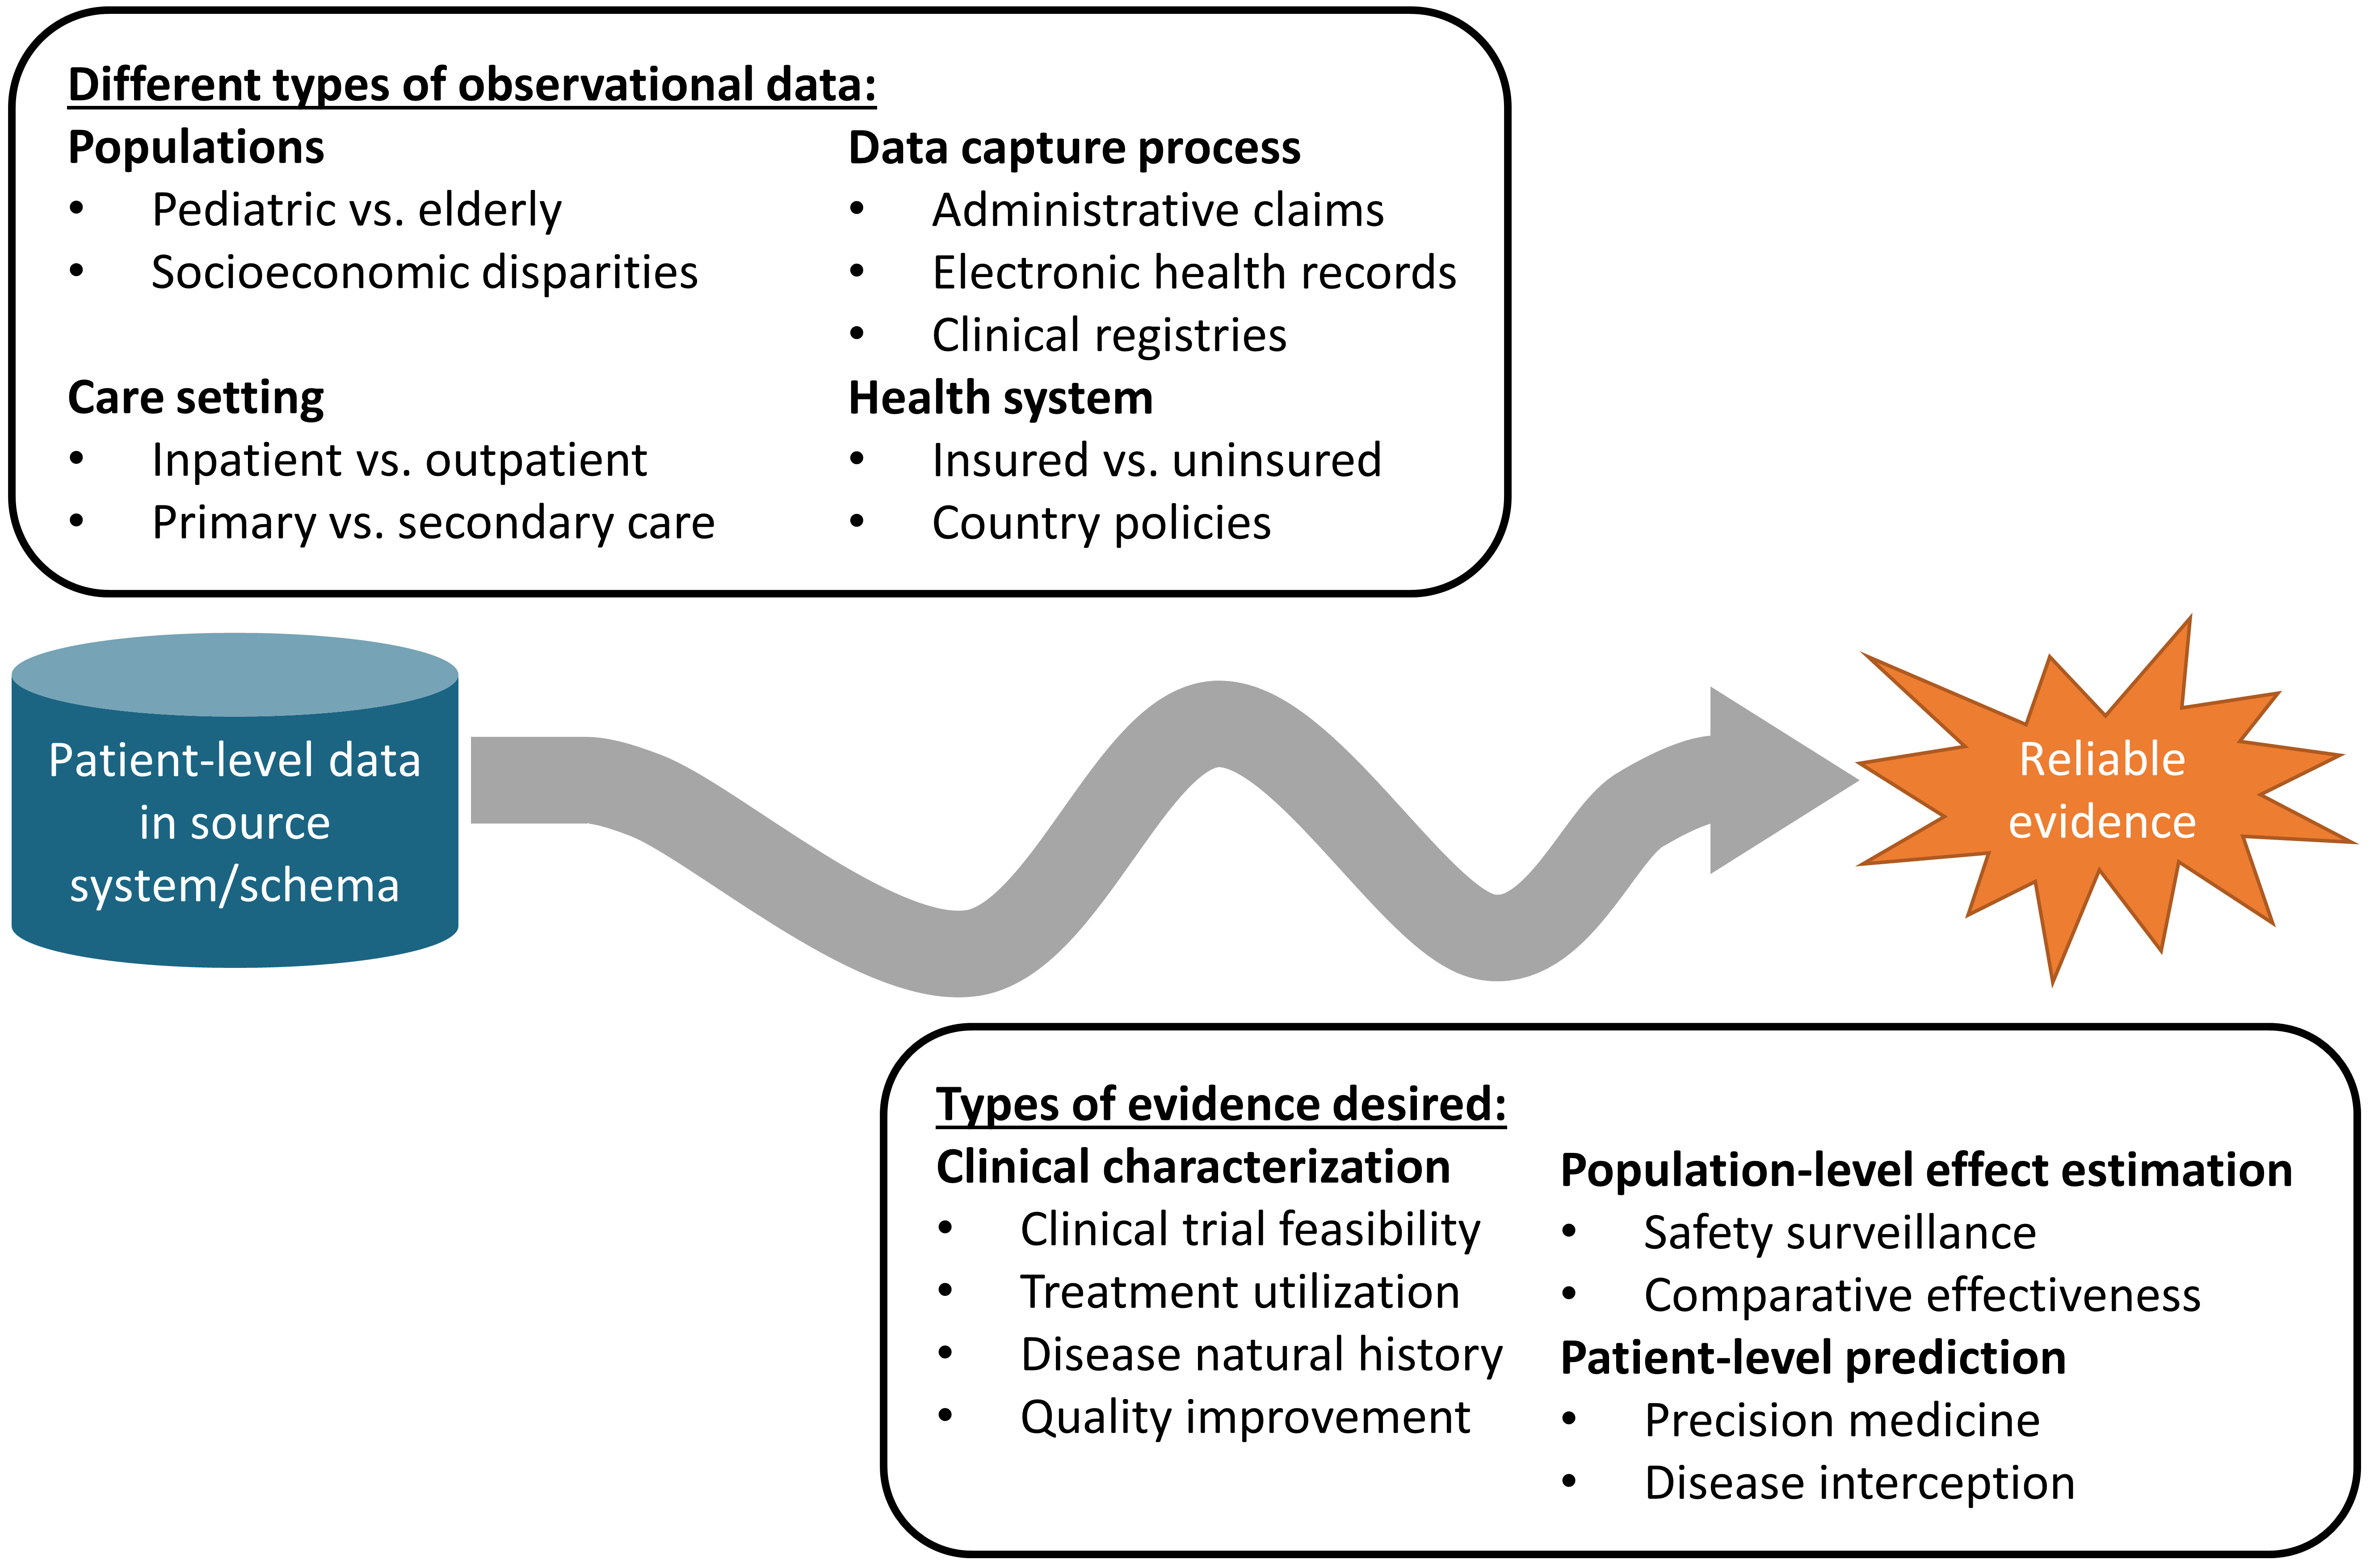
\includegraphics[width=1\linewidth]{images/OhdsiCommunity/datajourney} 

}

\caption{データからエビデンスへの旅}\label{fig:datajourney}
\end{figure}

ソースシステムには、さまざまな患者レベルのデータを収集するさまざまなタイプの観察データベースがあります。これらのデータベースは、医療システム自体と同様に多様であり、異なる集団、医療環境、データ収集プロセスを反映しています。意思決定に役立つエビデンスにもさまざまな種類があり、臨床的特性、集団レベルの推定、患者レベルの予測などの分析のユースケースによって分類することができます。 出発点(ソースデータ)と目的の目的地(エビデンス)とは別に、この課題はそのプロセスに必要とされる臨床、科学、技術的な能力の幅広さによってさらに複雑化しています。医療情報学を徹底的に理解する必要があります。これには、患者と医療従事者との診療現場でのやり取りから、管理システムや臨床システムを経て最終的な保存場所に至るまでのソースデータの完全な由来、データ収集や管理プロセスに関連する医療政策や行動インセンティブの一部として生じる可能性のある偏りへの理解が含まれます。臨床上の疑問を、適切な回答を得るのに適した観察研究のデザインに変換するための疫学の原則と統計的手法を習得する必要があります。何年にもわたる縦断的追跡調査で得られた何億件もの臨床の観察結果を含む、何百万人もの患者データセットに対して、計算効率の高いデータサイエンスアルゴリズムを実装し、実行する技術的能力が必要です。 また、観察データネットワークで得られた結果と他の情報源からのエビデンスを統合し、この新しい知識が医療政策や実臨床にどのような影響を与えるべきかを判断する臨床的知識も必要です。したがって、データからエビデンスを導くために必要なスキルとリソースとを備えている人物は非常にまれです。むしろ、このプロセスには、すべての利害関係者が信頼し意思決定プロセスに活用できるエビデンスを生成するために、最良のデータが最適な方法で分析されるよう、複数の個人や組織が協力することが必要となる場合がほとんどです。

\section{観察医療アウトカムパートナーシップ(OMOP)}\label{ux89b3ux5bdfux533bux7642ux30a2ux30a6ux30c8ux30abux30e0ux30d1ux30fcux30c8ux30caux30fcux30b7ux30c3ux30d7omop}

観察研究におけるコラボレーションの顕著な例として、Observational Medical Outcomes Partnership(OMOP)が挙げられます。OMOPは官民パートナーシップで、米国食品医薬品局(FDA)が主導し、米国立衛生研究所(NIH)財団が運営し、製薬会社からなるコンソーシアムが資金を提供しました。製薬会社は学術研究者や医療データパートナーと協力し、観察医療データを使用した積極的な医薬品安全性監視の科学を推進する研究プログラムを確立しました \citep{stang2010omop} 。 OMOPは、多様なステークホルダーによるガバナンス体制を確立し、真の医薬品安全性の関連性を特定し、偽陽性所見と区別するという課題に対して、さまざまな医療請求データやEHRデータベースに適用した場合の、代替となる疫学デザインや統計的手法のパフォーマンスを実証的に検証するための一連の方法論的実験を設計しました。

チームは集中型環境と分散型研究ネットワークの両方で、異なる観察データベースにまたがって研究を行うことの技術的な難しさを認識し、観察データの構造、内容、意味を標準化し、統計分析コードを一度作成すればすべてのデータサイトで再利用できるようにする仕組みとして、OMOP共通データモデル(CDM)を設計しました \citep{overhage2012cdm} 。OMOPの実験により、異なる医療現場から得られた異なるデータタイプを、異なるソース用語で表現し、施設間の連携と計算効率の高い分析を促進する方法で取り込むことができる共通データモデルと標準ボキャブラリを確立できることが実証されました。

OMOPは設立当初からオープンサイエンスのアプローチを採用し、研究デザイン、データ標準、分析コード、実証結果など、すべての成果物をパブリックドメインに置くことで透明性を高め、OMOPが実施している研究に対する信頼を構築するとともに、他者の研究目的の推進に再利用可能なコミュニティリソースを提供してきました。OMOPの当初の焦点は医薬品の安全性でしたが、OMOP CDMは、医療介入や医療制度政策の有効性の比較など、より広範な分析事例をサポートするために継続的に進化してきました。

OMOPは、大規模な実証実験の完了\citep{ryan2012omop, ryan2013omop} 、方法論の革新\citep{schuemie_2014}、安全性に関する意思決定のための観察データの適切な利用に役立つ知識の創出\citep{madigan_2013, madigan2013design}に成功しましたが、OMOPの遺産は、オープンサイエンスの原則を早期に採用し、OHDSIコミュニティの形成を促したという点で、より記憶されるかもしれません。

OMOPプロジェクトが完了し、FDAのアクティブサーベイランス活動に情報を提供するための方法論的研究という使命を果たしたとき、チームはOMOPの旅路が終わり、新たな旅路が始まったことを認識しました。OMOPの方法論的研究は、観察データから生成されるエビデンスの質を明らかに改善できる科学的ベストプラクティスに関する具体的な洞察を提供しましたが、それらのベストプラクティスの採用は遅々として進みませんでした。いくつかの障壁が特定されました。1)分析の革新よりも優先して取り組むべきであると考えられていた観察データの品質に関する根本的な懸念、2)方法論上の問題と解決策に対する概念的理解の不足、3)各自のローカル環境で独自に解決策を実行できないこと、4)これらのアプローチが各自の関心のある臨床問題に適用できるかどうかといった不確実性、などです。すべての障壁に共通する要素は、自分一人だけでは変化をもたらすために必要なすべてを持っているわけではないという感覚であり、しかし、何らかの協力的な支援があれば、すべての問題を克服できるというものでした。とはいえ、いくつかの分野でのコラボレーションが必要でした。

\begin{itemize}
\tightlist
\item
  オープンコミュニティのデータ標準、標準化されたボキャブラリ、ETL(抽出-変換-ロード)規約の確立に向けたコラボレーション。これにより、基礎となるデータ品質に対する信頼性が高まり、構造、内容、意味論の一貫性が促進され、標準化された分析が可能になります。
\item
  医薬品の安全性に留まらず、臨床的特性、集団レベルの推定、患者レベルの予測など、より広範なベストプラクティスを確立するための方法論的研究におけるコラボレーション。方法論的研究により実証された科学的ベストプラクティスを体系化し、研究コミュニティが容易に採用できる公開ツールとして利用可能にするためのオープンソース分析開発におけるコラボレーション。
\item
  コミュニティ全体で関心のある重要な健康問題に対処する臨床応用に関するコラボレーション。データからエビデンスへの道のりを共にたどる。
\end{itemize}

このような洞察から、OHDSIは誕生しました。

\section{オープンサイエンスの協働組織としてのOHDSI}\label{ux30aaux30fcux30d7ux30f3ux30b5ux30a4ux30a8ux30f3ux30b9ux306eux5354ux50cdux7d44ux7e54ux3068ux3057ux3066ux306eohdsi}

Observational Health Data Sciences and Informatics(OHDSI、発音は「オデッセイ」)は、コミュニティが協力してより良い医療判断とケアを促進するエビデンスを生成することで、健康の改善を目指すオープンサイエンスのコミュニティです\citep{Hripcsak2015}。OHDSIは、観察医療データの適切な利用に関する科学的ベストプラクティスを確立するための方法論的研究を実施し、これらのプラクティスを一貫性があり、透明性が高く、再現可能なソリューションに体系化するオープンソースの分析ソフトウェアを開発し、臨床上の疑問に適用してエビデンスを生成し、医療政策と患者ケアの指針となることを目指しています。

\subsection{我々の使命}\label{ux6211ux3005ux306eux4f7fux547d}

\begin{quote}
健康に関する意思決定とケアを向上させるエビデンスを協力して生成することにより、コミュニティをエンパワーメントし、健康を改善する。 \index{mission}
\end{quote}

\subsection{我々のビジョン}\label{ux6211ux3005ux306eux30d3ux30b8ux30e7ux30f3}

\begin{quote}
観察研究によって健康と疾病に関する包括的な理解が得られる世界。 \index{vision}
\end{quote}

\subsection{我々の目標}\label{ux6211ux3005ux306eux76eeux6a19}

\begin{itemize}
\item
  \textbf{革新性}: 観察研究は、革新的な恩恵を得ることができる分野です。我々の仕事において、新しい方法論的アプローチを積極的に探求し、奨励します。
\item
  \textbf{再現性}: 正確で再現可能な、適切に調整されたエビデンスが健康の改善に不可欠です。
\item
  \textbf{コミュニティ}: 患者、医療従事者、研究者、そして私たちの活動に賛同する方など、誰もがOHDSIに積極的に参加いただけます。 \index{community}
\item
  \textbf{コラボレーション}: 私たちは協力して、コミュニティの参加者の現実的なニーズを優先し、対処するために協力して取り組んでいます。
\item
  \textbf{オープン性}: 私たちは私たちが生み出す方法、ツール、生成されたエビデンスなど、コミュニティの成果をすべて公開し、一般にアクセスできるよう努めています。
\item
  \textbf{有益性}: コミュニティ内の個人や組織の権利を常に保護するよう努めています。 \index{objectives}
\end{itemize}

\section{OHDSIの進展}\label{ohdsiux306eux9032ux5c55}

OHDSIは2014年の発足以来、学術界、医療製品業界、規制当局、政府、保険者、技術提供者、医療システム、臨床医、患者など、さまざまなステークホルダーから2,500人以上のコラボレーターをオンラインフォーラムに迎え入れてきました。また、コンピュータサイエンス、疫学、統計学、生物医学情報学、医療政策、臨床科学など、さまざまな分野を代表する参加者もいます。OHDSIのコラボレーターのリストは、OHDSIのウェブサイトで閲覧できます\footnote{\url{https://www.ohdsi.org/who-we-are/collaborators/}}。 OHDSIの協力者マップ(図 \ref{fig:collaboratormap})は、国際的なコミュニティの広さと多様性を示しています。

\begin{figure}

{\centering 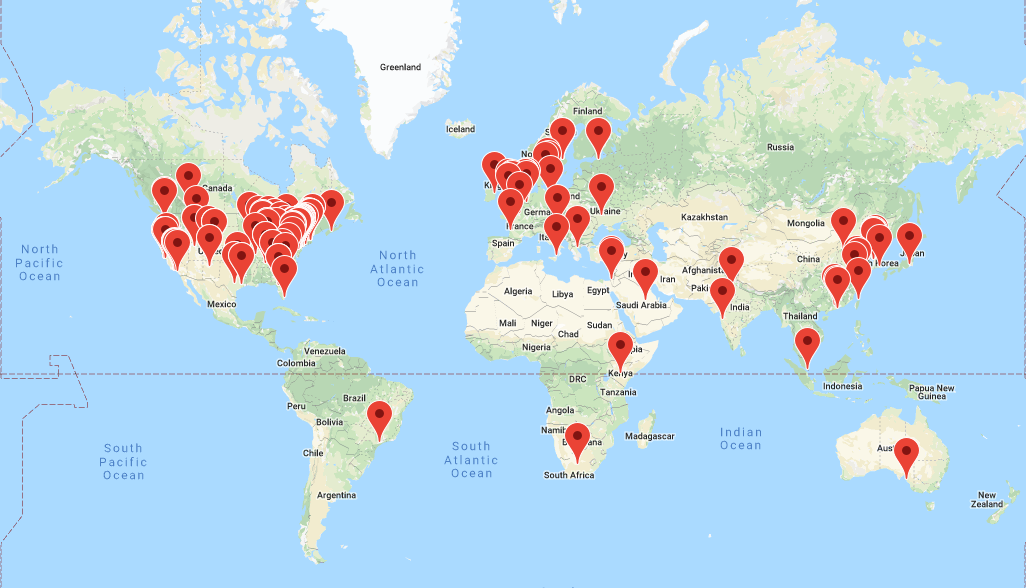
\includegraphics[width=1\linewidth]{images/OhdsiCommunity/mapOfCollaborators} 

}

\caption{2019年8月現在のOHDSI協力者の地図}\label{fig:collaboratormap}
\end{figure}

2019年8月現在、OHDSIは20か国以上から100以上の異なる医療データベースのデータネットワークを構築し、OMOP CDMというOHDSIが維持するオープンコミュニティデータ標準を用いた分散型ネットワークアプローチを適用することで10億件以上の患者レコードを収集しています。分散型ネットワークとは、患者レベルのデータを組織間で共有する必要がないことを意味します。代わりに、研究に関する問いはコミュニティ内の個人によって研究プロトコルの形で提起され、エビデンスを生成する分析コードが添付されます。生成されたデータは要約統計として共有され、研究に参加するパートナー間でのみ共有されます。OHDSIの分散型ネットワークを通じて、各データパートナーは患者レベルのデータの使用について完全な自主性を維持し、それぞれの機関のデータガバナンス方針を遵守し続けます。

OHDSIの開発者コミュニティは、OMOP CDMを基盤として、以下の3つのユースケースをサポートする堅牢なオープンソース分析ツールのライブラリを作成しました:1) 疾病の自然史、治療実態、品質向上のための臨床的特性評価;2) 医療製品の安全性監視と効果比較のための因果推論法を適用した集団レベルの効果推定;3) 精密医療や疾病予防のための機械学習アルゴリズムを適用する患者レベルの予測。OHDSIの開発者らは、OMOP CDMの採用、データの品質評価、OHDSIネットワーク研究の促進を支援するアプリケーションも開発しています。これらのツールには、RとPythonで作成されたバックエンドの統計パッケージや、HTMLとJavascriptで開発されたフロントエンドのウェブアプリケーションが含まれます。すべてのOHDSIツールはオープンソースであり、GitHubを通じて一般公開されています\footnote{\url{https://github.com/OHDSI}}。

OHDSIのオープンサイエンスコミュニティアプローチとオープンソースツールにより、観察研究は飛躍的に進歩しました。OHDSIネットワーク分析の初期の成果の一つとして、糖尿病、うつ病、高血圧という3つの慢性疾患の治療経路に関する調査が挙げられます。これはNational Academy of Scienceに掲載され、2億5000万人以上の患者データを対象とした11のデータソースから得られた結果を分析し、これまでに観察されたことのない治療選択に関する地理的な違いや患者の異質性を明らかにしました \citep{Hripcsak7329} 。OHDSIは交絡因子調整のための新しい統計的手法\citep{tian_2018}や因果推論のための観察的エビデンスの妥当性評価\citep{schuemie_2018}など、複数の分野でこれらのアプローチを適用しています。てんかんの安全性監視に関する問題\citep{duke_2017}から第二選択の糖尿病治療薬の効果比較\citep{vashisht_2018}や、うつ病治療の安全性比較に関する大規模な集団レベルの効果推定研究\citep{schuemie_2018b}に至るまで、さまざまな分野で適用されています。OHDSIコミュニティは、観察医療データに機械学習アルゴリズムを適用する方法の枠組みも確立しており\citep{reps2018}、さまざまな治療領域で適用されています\citep{johnston_2019, cepeda_2018, reps_2019}。

\section{OHDSIにおける協力}\label{ohdsiux306bux304aux3051ux308bux5354ux529b}

OHDSIはエビデンスを生成するためのコラボレーションを促進することを目的としたコミュニティです。OHDSIのコラボレーターになることにはどういう意味があるのでしょうか?もしあなたがOHDSIのミッションに賛同し、データからエビデンスを生む出すまでの過程のどこかに貢献したいと思うなら、OHDSIは最適なコミュニティです。コラボレーターには、患者レベルのデータにアクセスでき、そのデータがエビデンス生成に活用されることに興味を持つ人も含まれます。コラボレーターには、科学的ベストプラクティスを確立し、代替アプローチを評価したいという方法論者も含まれます。コラボレーターには、プログラミングスキルを活かしてコミュニティ全体が利用できるツール開発に関心を持つソフトウェア開発者も含みます。コラボレーターには、重要な公衆衛生上の疑問を持ち、それに対するエビデンスを広範な医療コミュニティに提供したいと考える臨床研究者も含まれます。コラボレーターには、この共通の公衆衛生のための目的を信じ、コミュニティが自立し、そのミッションを継続できるリソースを提供したいと思う個人や組織が含まれます。また、世界中でコミュニティ活動やトレーニングセッションを主催することも含まれます。OHDSIは専門分野やステークホルダーの所属に関わらず、共通の目的に向かった個人が協力し、それぞれが貢献することで、医療の進歩に寄与できる場となることを目指しています。この取り組みに参加したい方は第 \ref{WhereToBegin} 章(「どこから始めようか」)を参照し、参加方法をご確認ください。

\section{まとめ}\label{ux307eux3068ux3081}

\begin{rmdsummary}
\begin{itemize}
\item
  OHDSIのミッションは、健康に関する意思決定とケアを向上させるエビデンスを協力して生成することにより、コミュニティをエンパワーメントし、健康を改善させることです。
\item
  私たちのビジョンは、観察研究が健康と疾患に関する包括的な理解をもたらす世界であり、これを革新、再現性、コミュニティ、コラボレーション、オープン性、有益性の目標を通じて達成します。
\item
  OHDSIの協力者は、オープンコミュニティのデータ標準、方法論的研究、オープンソース分析の開発、臨床応用に重点的に取り組み、データからエビデンスへの旅を改善することに取り組んでいます。
\end{itemize}
\end{rmdsummary}

\chapter{--翻訳作業中-- どこから始めようか}\label{WhereToBegin}

\emph{章の著者:Hamed Abedtash \& Kristin Kostka}

\begin{quote}
「千里の道も一歩から」 - 老子
\end{quote}

OHDSIコミュニティは、学術界、産業界、政府機関といった多くの利害関係者で構成されています。私たちの仕事は患者、医療提供者、研究者、医療システム、産業界、政府機関など、さまざまな個人や組織に利益をもたらします。この利益は、医療データ分析の質を向上させるだけでなく、これらの利害関係者にとっての医療データの有用性を向上させることによって実現されます。私たちは、観察研究が革新的な思考から大いに恩恵を受ける分野だと考えており、積極的に新しい方法論的アプローチを模索し、奨励しています。

\section{旅に参加しよう}\label{ux65c5ux306bux53c2ux52a0ux3057ux3088ux3046}

OHDSIには、患者、医療専門家、研究者、あるいは私たちの活動に賛同する人など、誰もが積極的に参加できます。OHDSIは包括的なメンバーシップモデルを維持しています。OHDSIのコラボレーターになるために会費は必要ありません。コラボレーションは手を挙げるだけの簡単なもので、毎年のOHDSI会員数に含まれます。参加は完全に任意です。コラボレーターは、毎週のコミュニティコールに参加するだけの人から、ネットワーク研究やOHDSIワーキンググループを率いる人まで、さまざまなレベルの貢献が可能です。データ保持者でなくても、活発なコミュニティメンバーとして参加できます。OHDSIコミュニティは、データ保持者、研究者、医療提供者、患者や消費者に同様にサービスを提供することを目的としています。コラボレーターのプロファイルの記録はOHDSIウェブサイトで維持され、定期的に更新されます。メンバーシップはOHDSIコミュニティコール、ワーキンググループや地域支部によって促進されます。

\begin{figure}

{\centering 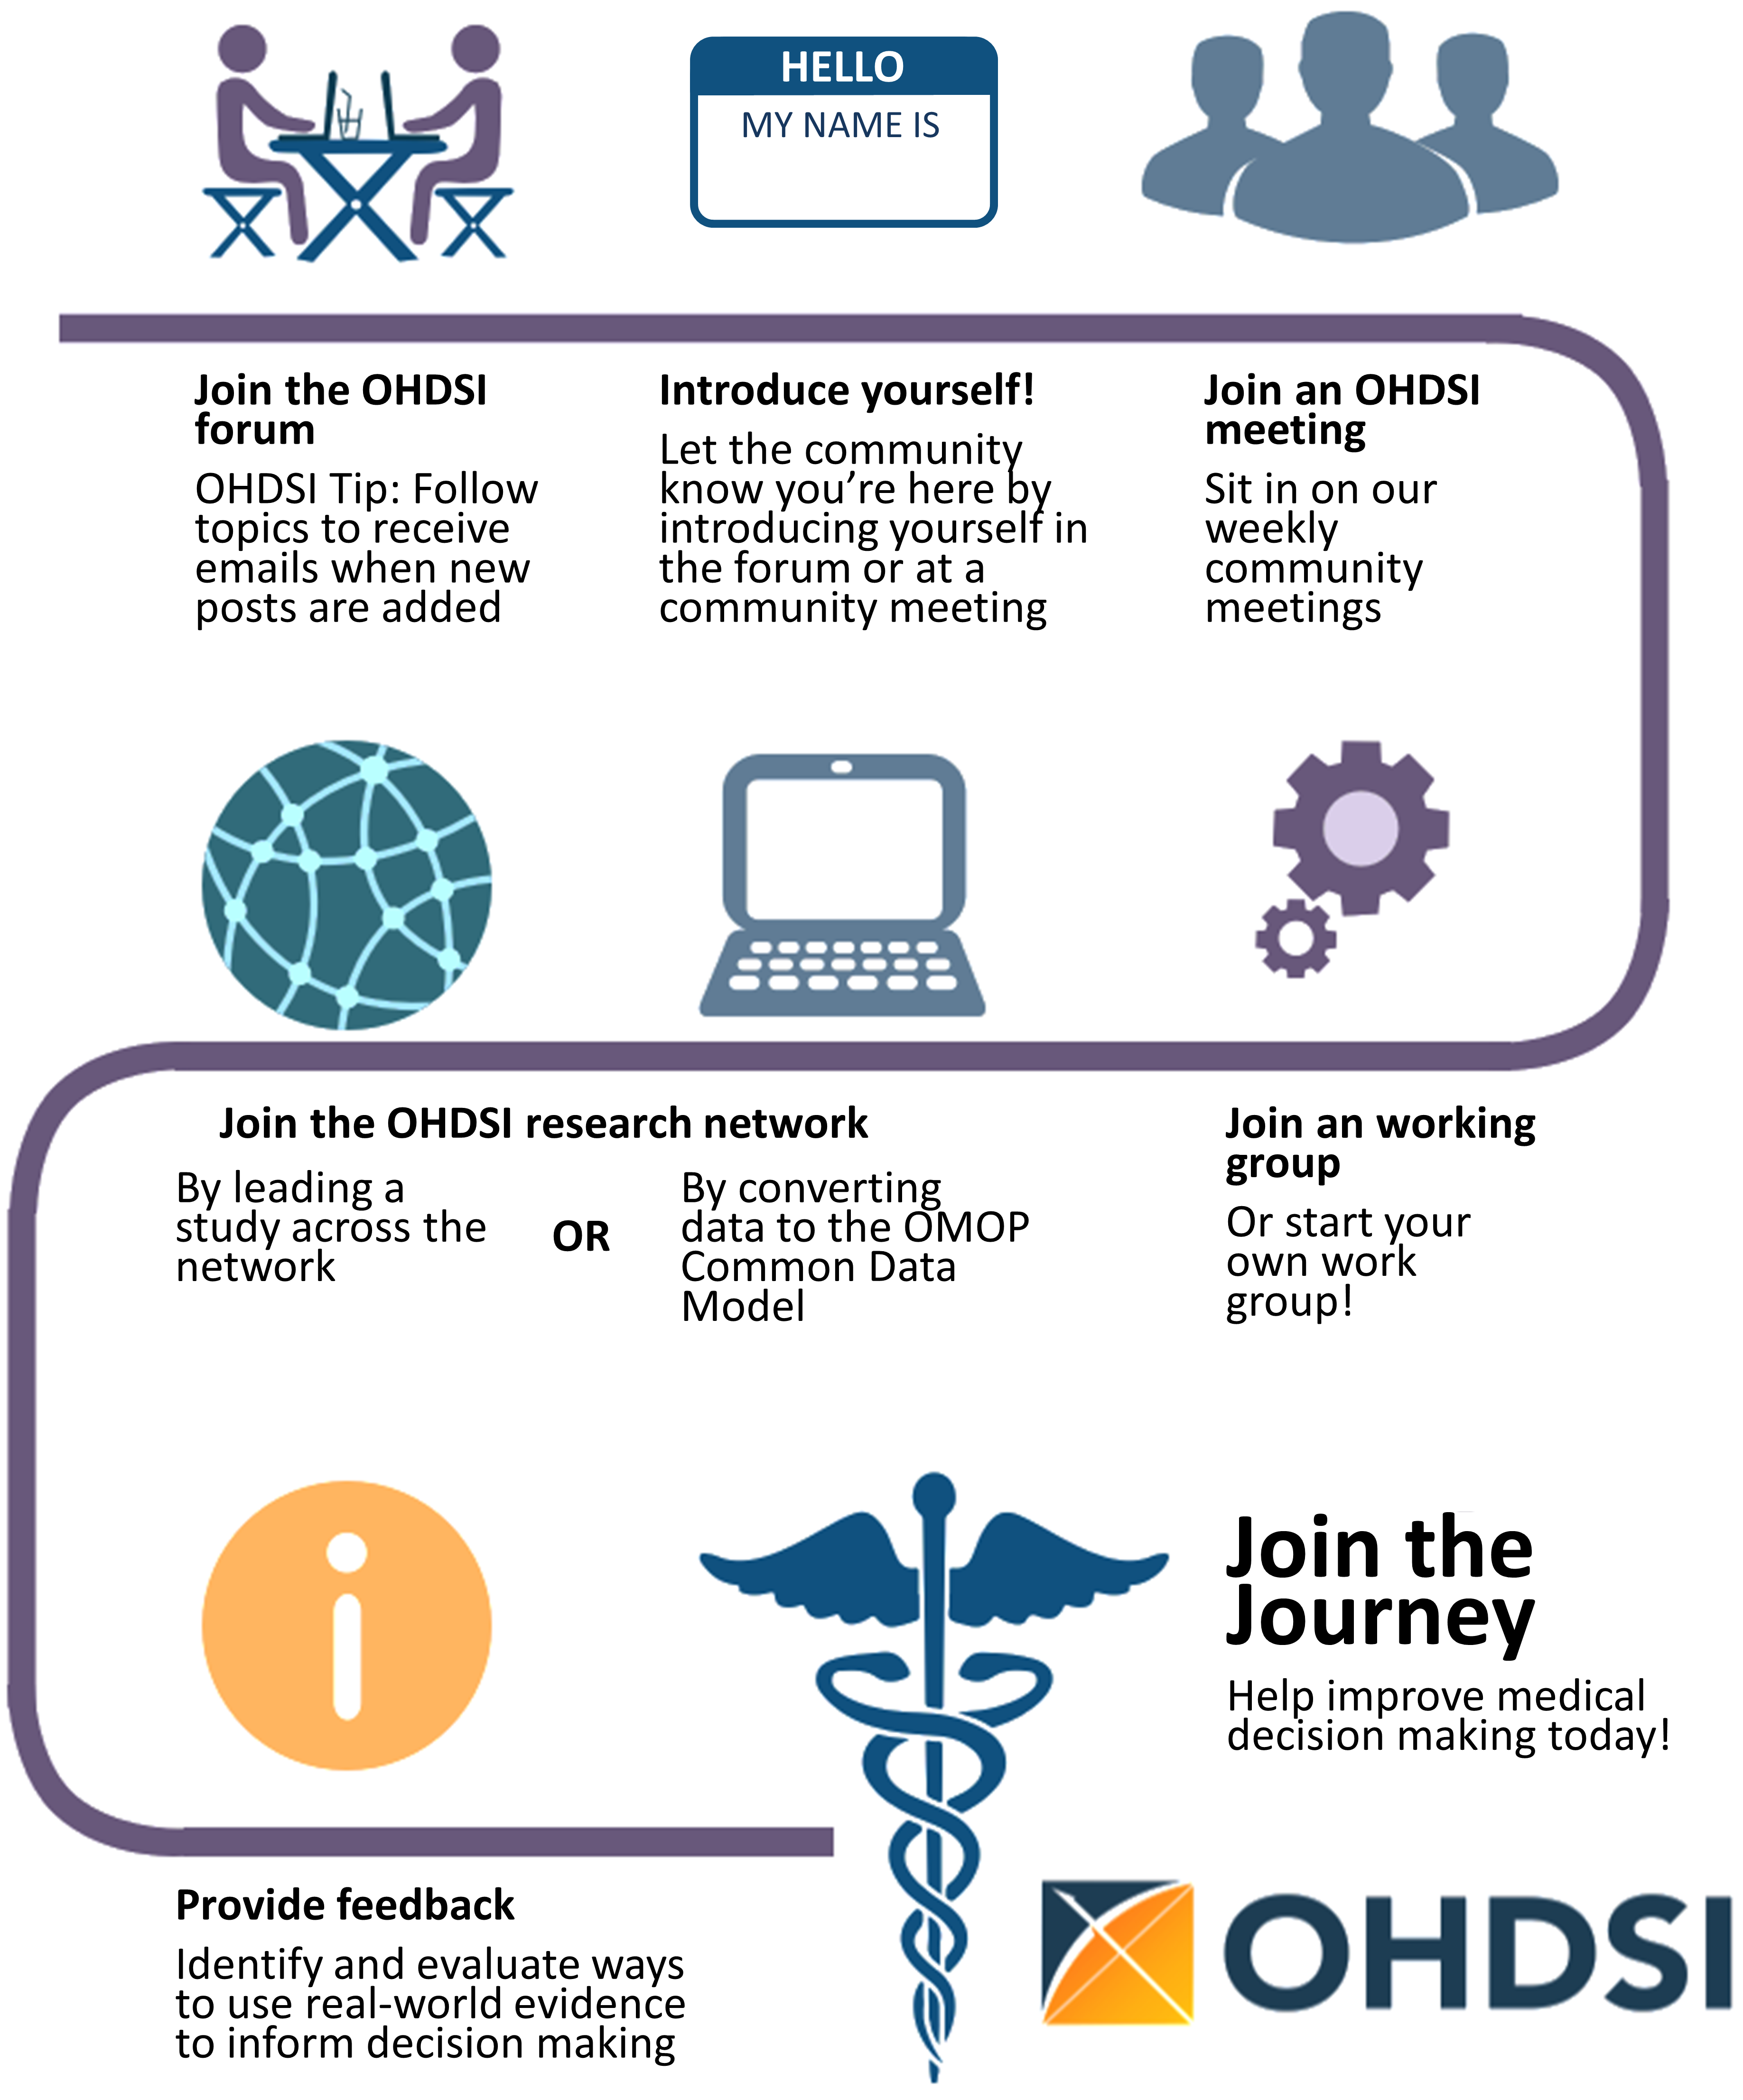
\includegraphics[width=0.9\linewidth]{images/WhereToBegin/joinTheJourney} 

}

\caption{旅に参加しよう ― OHDSIのコラボレーターになるには}\label{fig:jointhejourney}
\end{figure}

\subsection{OHDSIフォーラム}\label{ohdsiux30d5ux30a9ux30fcux30e9ux30e0}

OHDSIフォーラム\footnote{\url{https://forums.ohdsi.org}} は、OHDSIコミュニティのコラボレーターが投稿メッセージの形で会話ができるオンラインのディスカッションサイトです。フォーラムはツリー状のディレクトリ構造で構成されています。最上部は「カテゴリ」です。フォーラムは、関連するディスカッションのカテゴリで分けることができます。カテゴリの下にはサブフォーラムがあり、これらのサブフォーラムにはさらにサブフォーラムがあります。トピック(一般にはスレッドと呼ばれる)はサブフォーラムの最下層にあり、ここでフォーラムメンバーはディスカッションや投稿を始められます。

OHDSIフォーラムには、次のようなコンテンツのカテゴリがあります:

\begin{itemize}
\tightlist
\item
  \textbf{一般:} OHDSIコミュニティに関する一般的なディスカッションと参加方法
\item
  \textbf{実装者:} 共通データモデルとOHDSI分析フレームワークをローカル環境に実装する方法についてのディスカッション
\item
  \textbf{開発者:} OHDSIアプリケーションや他のOMOP CDMを活用するツールのオープンソース開発についてのディスカッション
\item
  \textbf{研究者:} CDMベースの研究に関するディスカッション(エビデンス生成、共同研究、統計手法やOHDSI研究ネットワークに関連するその他のトピックを含む)
\item
  \textbf{CDMビルダー:} 要件、ボキャブラリ、技術的側面を含む進行中のCDM開発に関するディスカッション
\item
  \textbf{語彙ユーザー:} ボキャブラリコンテンツに関するディスカッション
\item
  \textbf{地域支部(例:韓国、中国、ヨーロッパ):} OMOP実装やOHDSIコミュニティ活動に関連する、母国語での地域のディスカッション
\end{itemize}

自分のトピックを投稿するには、アカウントにサインアップする必要があります。フォーラムのアカウントを取得し、一般的なトピックの「Welcome to OHDSI! - Please introduce yourself(OHDSIへようこそ!-自己紹介をお願いします」というスレッドで自己紹介することをお勧めします。返信では1) 自己紹介と自分の仕事について簡単に教えてください、2) コミュニティでどのように貢献したいか教えてください(例:ソフトウェア開発、研究実施、研究論文の執筆など)。これでOHDSIの旅が始まります!ここから、ディスカッションに参加することをお勧めします。質問したり、新しいアイデアを議論したり、コラボレーションしたりするための手段として、OHDSIコミュニティはフォーラムを使用することを推奨しています。 \index{forum}

\begin{rmdimportant}
トピックを選択して「ウォッチ」することができます。ウォッチしているトピックに新しい投稿が追加されるたびにメールが届き、その投稿にメールで直接返信できるようになります。一般的なスレッドをウォッチして、今後の会議の議題や、コラボレーションの機会に関する詳細を受け取ったり、毎週のOHDSIダイジェストを直接受信トレイに配信しましょう!
\end{rmdimportant}

\subsection{OHDSIイベント}\label{ohdsiux30a4ux30d9ux30f3ux30c8}

OHDSIは、コラボレーター同士が学び合い、将来の協力を促進する機会を提供するため、定期的に対面イベントを開催しています。これらのイベントはOHDSIウェブサイトで通知され、参加を希望する人は誰でも無料で参加できます。

OHDSIシンポジウムは、米国、ヨーロッパ、アジアで毎年開催される学術会議で、コラボレーターが全体会議、ポスター発表、ソフトウェアのデモを通じて最新の研究を発表できます。OHDSIシンポジウムはネットワーキングのための素晴らしい場であり、コミュニティ全体での最新の進歩について学ぶ機会です。OHDSIシンポジウムには通常、OHDSIチュートリアルが併設されており、OHDSI 共同研究者がOHDSI 共同研究者がコースの講師となって教えるもので、コミュニティの新規参加者に、データ標準や分析のベストプラクティスに関するトピックについて実践的な取り組みを行う機会を提供します。これらのチュートリアルは通常ビデオ録画され、イベント後にOHDSIウェブサイトで公開され、イベントに参加できなかった人も利用できます。

OHDSIコラボレーターの対面イベントは、通常は共通の関心事の問題に焦点を当てた小規模なフォーラムです。過去のイベントには、フェノタイプ・ハッカソン、データ品質ハッカソン、オープンソースソフトウェアのドキュメンテーション・ハッカソンなどがあります。OHDSIは、複数のStudy-a-thonイベントを主催してきました。この複数日にわたるセッションの目的は、適切な観察分析を設計・実装し、OHDSIネットワーク全体で研究を実行し、一般への普及のためにエビデンスを統合することにより、特定の研究問題に関してチームとして協力することです。これらのすべてのイベントにおいて、共通の問題を解決したいという共通の願いがあるだけでなく、共同で問題解決を行うプロセスを学び、継続的な改善を促す歓迎的な環境を提供することにも共通の関心があります。

OHDSIコミュニティのパワーをもっと学びましょう。過去のシンポジウム、対面会議を検索し、OHDSIチュートリアルを視聴ください。OHDSIウェブサイトの\href{https://www.ohdsi.org/past-events/}{過去のイベント}セクションから視聴できます。過去のイベントは定期的に更新され、コミュニティイベントはアーカイブされています。

\subsection{OHDSIコミュニティコール}\label{ohdsiux30b3ux30dfux30e5ux30cbux30c6ux30a3ux30b3ux30fcux30eb}

OHDSI コミュニティ コールは、OHDSI コミュニティ内で進行中の活動にスポットライトを当てる機会です。毎週火曜日の午前11時から12時(東部標準時)に開催される電話会議は、OHDSIコミュニティが集まり、最近の開発を共有し、個々のコラボレーター、ワーキンググループ、コミュニティ全体の成果を認識する時間です。毎週の会議は記録され、プレゼンテーションはOHDSIウェブサイトのリソースにアーカイブされます。

OHDSIコラボレーターは、毎週の電話会議への参加を歓迎され、コミュニティディスカッションのトピックを提案することが奨励されています。OHDSIコミュニティコールは、研究成果を共有し、進行中の作業に対するフィードバックを求め、開発中のオープンソースソフトウェアツールをデモンストレーションし、データモデリングと分析のためのコミュニティベストプラクティスを議論し、助成金/出版物/会議ワークショップのための将来のコラボレーションの機会をブレインストーミングするフォーラムとなります。OHDSIコラボレーター会議のトピックを持っているコラボレーターは、OHDSIフォーラムに意見を投稿ください。

OHDSI コミュニティの新規参加者として、OHDSIネットワーク全体で何が起こっているかを把握するために、このコールシリーズをカレンダーに追加することをお勧めします。OHDSIコールに参加する場合は、OHDSIフォーラムでアナウンスを確認してください。\href{https://forums.ohdsi.org/}{OHDSIフォーラム}コミュニティコールのトピックは週ごとに異なります。OHDSIフォーラムのOHDSIウィークリーダイジェストで、毎週のプレゼンテーションのトピックの詳細情報を確認することもできます。新規参加者は、初回のコールで自己紹介し、自分自身、経歴、OHDSIに参加した理由についてコミュニティに話すよう求められます。\index{コミュニティ!コミュニティコール}

\subsection{OHDSIワークグループ}\label{ohdsiux30efux30fcux30afux30b0ux30ebux30fcux30d7}

OHDSI には、ワークグループチームが主導するさまざまな進行中のプロジェクトがあります。各ワークグループにはそれぞれリーダーシップ チームがあり、プロジェクトの目的、目標、コミュニティに提供される成果物を決定します。ワークグループには、プロジェクトの目的と目標に貢献することに関心のあるすべての人が参加できます。ワークグループは、長期にわたる戦略的な目的の場合もあれば、コミュニティの特定のニーズを満たすための短期プロジェクトである場合もあります。ワークグループの会議の頻度は、プロジェクトリーダーシップによって決定され、グループごとに異なります。アクティブなワークグループのリストは、\href{https://www.ohdsi.org/web/wiki/doku.php?id=projects:overview}{OHDSI Wiki} \index{workgroups}で管理されています。

表 \ref{tab:OHDSIworkgroups} は、アクティブなOHDSI作業グループのクイックリファレンスです。是非コールに参加して、より多くを学ぶことをお勧めします。

\begin{longtable}[]{@{}
  >{\raggedright\arraybackslash}p{(\columnwidth - 4\tabcolsep) * \real{0.3333}}
  >{\raggedright\arraybackslash}p{(\columnwidth - 4\tabcolsep) * \real{0.3333}}
  >{\raggedright\arraybackslash}p{(\columnwidth - 4\tabcolsep) * \real{0.3333}}@{}}
\caption{\label{tab:OHDSIworkgroups} 注目すべきOHDSI作業グループ}\tabularnewline
\toprule\noalign{}
\begin{minipage}[b]{\linewidth}\raggedright
ワークグループ名
\end{minipage} & \begin{minipage}[b]{\linewidth}\raggedright
目的
\end{minipage} & \begin{minipage}[b]{\linewidth}\raggedright
対象参加者
\end{minipage} \\
\midrule\noalign{}
\endfirsthead
\toprule\noalign{}
\begin{minipage}[b]{\linewidth}\raggedright
ワークグループ名
\end{minipage} & \begin{minipage}[b]{\linewidth}\raggedright
目的
\end{minipage} & \begin{minipage}[b]{\linewidth}\raggedright
対象参加者
\end{minipage} \\
\midrule\noalign{}
\endhead
\bottomrule\noalign{}
\endlastfoot
Atlas \& WebAPI & AtlasとWebAPIは、OMOP共通データモデルを基盤として構築し、標準化された分析機能を提供するOHDSIオープンソースソフトウェアアーキテクチャの一部です。 & オープンソースのAtlas/WebAPIプラットフォームを改善し、貢献することを目指すJava \& JavaScriptソフトウェア開発者 \\
CDM \& ボキャブラリ & 臨床患者データに適用される体系的で、標準化された大規模な分析を目的として、OMOP共通データモデルの開発を継続します。他のワーキング グループによって開発された標準化された分析をサポートするため、国際的なコーディングシステムと患者ケアの臨床的側面のカバレッジを拡大することで、標準化されたボキャブラリの品質を向上させます。 & OMOP共通データモデルと標準ボキャブラリの改善に関心があり、すべてのニーズとユースケースに対応できる人 \\
ゲノム解析 & OMOP CDMを拡張して、患者のゲノムデータを組み込みます。グループは、さまざまなシーケンスプロセスからの遺伝子変異に関する情報を保存できる CDM 互換スキーマを定義します。 & すべての人が参加可能 \\
集団レベルの推定 & 正確で信頼性が高く、再現性のある集団レベルの効果推定につながる観察研究のための科学的手法を開発し、コミュニティによるこれらの手法の使用を促進します。 & すべての人が参加可能 \\
自然言語処理 & OHDSI傘下の観察研究で、電子健康記録(EHR)のテキスト情報の使用を促進します。この目的を促進するため、グループはOHDSIコミュニティによる研究に臨床テキストを利用するために実装できる方法とソフトウェアを開発します。 & すべての人が参加可能 \\
患者レベルの予測 & 複数の対象とするアウトカムに用いることができ、対象とするあらゆる患者サブグループからの観察医療データに適用します。正確で十分に調整された患者中心の予測モデルを開発するため、標準化されたプロセスを確立します。 & すべての人が参加可能 \\
ゴールドスタンダート表現型ライブラリ & OHDSIコミュニティのメンバーが、コミュニティで検証されたコホート定義を研究やその他の活動のために見つけ、評価し、利用できるようにします。 & フェノタイプのキュレーションと検証に関心のあるすべての人が参加可能 \\
FHIR ワークグループ & OHDSI FHIR統合のロードマップを確立し、OHDSIベースの観察研究のためにEHRコミュニティのFHIR実装とデータを活用し、FHIRベースのツールとAPIを通じてOHDSIデータと研究結果を普及するための推奨事項を、より広範なコミュニティに提供します。 & 相互運用性に関心のあるすべての人が参加可能 \\
GIS & OMOP CDMを拡張し、患者の環境曝露の履歴をその臨床フェノタイプと関連付けるためにOHDSIツールを活用します。 & 健康関連の地理属性に興味のあるすべての人が参加可能 \\
臨床試験 & OHDSIプラットフォームとエコシステムがあらゆる面で試験を支援できる臨床試験のユースケースを理解し、サポートする OHDSI ツールの更新の推進を支援します。 & 臨床試験に興味のあるすべての人が参加可能 \\
THEMIS & THEMIS の目的は、OMOP CDM 規則を超える標準規則を開発し、各 OMOP サイトで設計された ETL プロトコルが最高品質で、再現可能かつ効率的であることを保証することです。 & ETL標準化に関心のあるすべての人が参加可能 \\
メタデータ \& 注釈 & 私たちの目標は、人間と機械が作成したメタデータと注釈を 共通データモデル に保存するための標準プロセスを定義し、研究者が観察データセットに関する有用なデータ成果物を利用して作成できるようにすることです。 & すべての人が参加可能 \\
患者生成医療データ (PGHD) & この ワーキンググループの目標は、スマートフォン/アプリ/ウェアラブル デバイスから生成される PGHD の ETL 規則、臨床データとの統合プロセス、分析プロセスを開発することです。 & すべての人が参加可能 \\
OHDSI女性グループ & OHDSIコミュニティ内の女性が一堂に会し、科学、技術、工学、数学(STEM)で働く女性として直面する課題について話し合う場を提供すること。OHDSIコミュニティがSTEM分野の女性をどのようにサポートできるかについて、女性たちが自分たちの視点を共有し、懸念を提起し、アイデアを提案し、最終的にはコミュニティやそれぞれの分野でリーダーとなる女性たちを鼓舞することができるような議論を促進することを目指しています。 & このミッションに賛同するすべての人が参加可能 \\
運営委員会 & OHDSIのすべての活動とイベントが、成長を続けるコミュニティのニーズに合致していることを確認することで、OHDSI の使命、ビジョン、価値観を維持します。さらに、このグループは、OHDSI の将来の方向性についてガイダンスを提供することで、コロンビアに拠点を置く OHDSI 調整センターの諮問グループとして機能します。 & コミュニティ内のリーダー \\
\end{longtable}

\subsection{OHDSI地域支部}\label{ohdsiux5730ux57dfux652fux90e8}

OHDSI 地域支部は、地理的な地域に所在し、地域特有の問題に対処するため、ローカル ネットワークイベントや会議を開催したいと考えている OHDSI コラボレーターのグループです。現在、OHDSI地域支部は、ヨーロッパ\footnote{\url{https://www.ohdsi-europe.org/}}、韓国\footnote{\url{https://forums.ohdsi.org/c/For-collaborators-wishing-to-communicate-in-Korean}}、中国\footnote{\url{https://ohdsichina.org/}}にあります。ご自身の地域で OHDSI 地域支部を設立したい場合は、OHDSI Webサイトで説明されているOHDSI地域支部のプロセスに従って設立できます。

\subsection{OHDSIリサーチネットワーク}\label{ohdsiux30eaux30b5ux30fcux30c1ux30cdux30c3ux30c8ux30efux30fcux30af}

OHDSI のコラボレーターの多くは、データをOMOP共通データモデルに変換することに関心を持っています。OHDSI研究ネットワークは、抽出、変換、ロード(ETL)プロセスを経てOMOPに準拠した観測データベースの多様なグローバルコミュニティを表しています。OHDSIコミュニティでの取り組みにデータの変換が含まれる場合は、OMOP CDMとボキャブラリに関するチュートリアル、変換を支援する無料で利用可能なツール、特定のドメインやデータ変換の種類を対象とするワークグループなど、取り組みを支援する多数のコミュニティリソースがあります。OHDSIのコラボレーターは、OHDSIフォーラムを利用して、CDM変換中に発生する課題について話し合い、トラブルシューティングすることを推奨されます。

\section{どこにフィットするか}\label{ux3069ux3053ux306bux30d5ux30a3ux30c3ux30c8ux3059ux308bux304b}

ここまで読んで、あなたは「私は OHDSI コミュニティのどこに属しているのだろう?」と疑問に思っているかもしれません。

\textbf{私は臨床研究者で、研究を始めたいと思っています。} 特定の質問に答えるためにOHDSIリサーチネットワークを使用したい臨床研究者であるなら、たとえば論文を発表したいと考えているなら、あなたは正しい場所にいます。OHDSIフォーラムの\href{https://forums.ohdsi.org/c/researchers}{OHDSIリサーチャーズトピック}にアイデアを投稿することから始めましょう。これにより、同様の関心を持つ研究者とつながることができます。OHDSIは論文の出版を好んでおり、リサーチクエスチョンを分析や迅速に分析や論文にしていくための多くのリソースを提供しています。詳細は第\ref{Characterization}、\ref{PopulationLevelEstimation}、\ref{PatientLevelPrediction}章をご覧ください。

\textbf{私はOHDSIコミュニティが発信する情報を読んで利用したいと思っています。} 患者、臨床医、医療の専門家のいずれであっても、OHDSI は健康アウトカムをよりよく理解するのに役立つ高品質のエビデンスを提供したいと考えています。コードを書くのは久しぶりかもしれません。プログラムを書いたことがないかもしれません。あなたにはこのコミュニティに居場所があります。私たちはあなたを\emph{エビデンスの消費者}と呼びます。あなたはOHDSIの研究を行動に移す人です。あなたは OHDSI がどのようなエビデンスを生成したか、または生成中であるかを知るためにふるいにかけており、おそらく自分に関連する質問を提案したいとも思っているでしょう。私たちはあなたがディスカッションに参加することを歓迎します。\href{http://forums.ohdsi.org}{OHDSIフォーラム}で質問を始めましょう。コミュニティコールに参加し、最新の研究について聞いてください。OHDSIシンポジウムや対面ミーティングに参加してコミュニティと直接交流しましょう。あなたの質問はOHDSIコミュニティの重要な部分です。声を上げて、あなたが探しているエビデンスについて、私たちがさらに知る手助けをしてください!

\textbf{私は医療のリーダーとして働いています。データ所有者、またはその代表者であるかもしれません。組織にとってのOMOP CDMとOHDSI分析ツールの有用性を評価しています。} 組織の管理者/リーダーとして、あなたはOHDSIについて聞いたことがあり、OMOP CDMがあなたのユースケースにどのように役立つかを知りたいと思っているかもしれません。\href{https://www.ohdsi.org/past-events/}{OHDSIの過去のイベント}資料に目を通し、研究内容を確認ください。コミュニティコールに参加して、ただ聞くだけでも構いません。 \ref{DataAnalyticsUseCases} 章(データ分析のユースケース)を読むと、OMOP CDMやOHDSI分析ツールで実現できる研究の種類を理解するのに役立つかもしれません。OHDSIコミュニティは、あなたの旅をサポートします。興味のある具体的な分野がある場合は遠慮せずに発言し、事例を尋ねてください。世界中の200以上の組織がOHDSIで協力しており、コミュニティの価値を示すための多くの成功事例があります。

\textbf{私はデータベース管理者で、私の機関のデータをETLまたはOMOP CDMに変換したいと考えています。} データを「OMOP」することは、斬新で価値のある取り組みです。ETLプロセスを始めたばかりの場合、\href{https://www.ohdsi-europe.org/images/symposium-2019/tutorials/OHDSI_Vocabulary_CDM_Tutorial.pdf}{OHDSIコミュニティのETLチュートリアルスライド}を参照するか、今後開催されるOHDSIシンポジウムに登録したりしてください。THEMIS作業グループのコールに参加し、OHDSIフォーラムで質問することも考えてみてください。OMOP CDMの実装を成功に導く支援となる知識がコミュニティには豊富にあります。遠慮しないでください!

\textbf{私はバイオ統計学者かつ、またはメソッドの開発者で、OHDSIツールスタックへの貢献に興味があります。}Rに精通しており、Gitにコミットする方法を知っています。何よりも、OHDSIメソッドライブラリに専門知識を持ち込み、これらの方法論をさらに発展させたいと思っています。まずは、集団レベルの推定または患者レベルの予測のワークグループコールに参加し、現在のコミュニティの優先事項について詳しく聞くことをお勧めします。OHDSIツールを使用する際、該当するGitHubリポジトリ(例:SQL Renderパッケージの問題であれば、OHDSI/SqlRenderのGitHubリポジトリに提出します)に問題を報告することもできます。皆さんの貢献をお待ちしています!

\textbf{私はソフトウェア開発者で、OHDSIツールスタックを補完するツールの構築に関心があります。} コミュニティへようこそ!OHDSIのミッションの一環として、私たちのツールはApacheライセンスの下でオープンソースとして管理されています。OHDSIツールスタックを補完するソリューションの開発を歓迎しています。ワーキンググループに参加し、アイデアを提案ください。OHDSIはオープンサイエンスとオープンコラボレーションに多大な投資をしていることに留意ください。独自のアルゴリズムとソフトウェアソリューションは歓迎しますが、私たちのソフトウェア開発の主な焦点ではありません。

\textbf{私はコンサルタントで、OHDSIコミュニティに助言したいと考えています。} コミュニティへようこそ!あなたの専門知識は貴重であり、高く評価されています。必要に応じて、OHDSIフォーラムでサービスを宣伝することができます。OHDSIチュートリアルに参加ください。また、年間を通じてシンポジウムの議事録や OHDSI の対面ミーティングで専門知識を提供して貢献することを検討ください。

\textbf{私は学生で、OHDSIについてもっと学びたいと思っています。} あなたは正しい場所にいます!OHDSIコミュニティコールに参加し、自己紹介することを考えてみてください。OHDSIチュートリアルを詳しく調べたり、OHDSIシンポジウムや対面ミーティングに参加してOHDSIコミュニティが提供する方法とツールについてさらに学ぶことをお勧めします。特定の研究に関心がある場合は、OHDSIフォーラムの研究者トピックに投稿してお知らせください。多くの組織がOHDSIが後援する研究の機会(例:ポスドク、研究フェローシップ)を提供しています。OHDSIフォーラムでは、これらの機会などに関する最新情報を提供しています。

\section{まとめ}\label{ux307eux3068ux3081-1}

\begin{rmdsummary}
\begin{itemize}
\tightlist
\item
  OHDSIコミュニティに参加するのは、挨拶するのと同じくらい簡単です。\textbf{OHDSIフォーラム}に投稿し、コミュニティコールに参加ください。
\item
  研究やETLに関する質問をOHDSIフォーラムに投稿ください。
\end{itemize}
\end{rmdsummary}

\chapter{--翻訳作業中-- オープンサイエンス}\label{OpenScience}

\index{オープンサイエンス}

\emph{章の著者:Kees van Bochove}

OHDSIコミュニティの発足当初から、オープンソースソフトウェアの利用、すべての会議の議事録や資料の公開、生成された医療的エビデンスの透明性あるオープンアクセスによる公開など、オープンサイエンスの価値観に基づいて国際的な共同研究体制を確立することが目標とされてきました。しかし、オープンサイエンスとは具体的にはどのようなものでしょうか? また、プライバシーへの配慮が非常に重要であり、通常は正当な理由から公開されない医療データに関してOHDSIはどのようにオープンサイエンスやオープンデータ戦略を構築できるのでしょうか。分析の再現性がなぜそれほど重要なのでしょうか。OHDSIコミュニティはこれをどのようにしてこれを実現しようとしているのでしょうか。 本章ではこれらの疑問について触れていきます。

\section{オープンサイエンス}\label{ux30aaux30fcux30d7ux30f3ux30b5ux30a4ux30a8ux30f3ux30b9}

「オープンサイエンス」という用語は1990年代から使われていましたが実際に注目を集めるようになったのは2010年代で、OHDSIが誕生したのと同じ時期です。Wikipedia \citep{wiki:Open_science} ではこれを「科学的研究(出版物、データ、物理的サンプル、ソフトウェアを含む)とその普及を、アマチュアか専門家を問わず、探求心のあるあらゆるレベルの人々が利用できるようにする運動」と定義しており、通常は共同ネットワークを通じて開発されると述べています。OHDSIコミュニティは明確には「オープンサイエンス」集団またはネットワークとして位置づけられたことはありませんが、この用語はOHDSIの基本的な概念や原則を説明する際に頻繁に使われています。例えば、2015年にはジョン・デュークがOHDSIを「医療エビデンス生成へのオープンサイエンスアプローチ」\footnote{\url{https://ohdsi.github.io/TheBookOfOhdsi/OpenScience.html\#fn17}}と表現し、2019年にはEHDENコンソーシアムの紹介ウェビナーでOHDSIネットワークアプローチを「21世紀のリアルワールドオープンサイエンス」\footnote{\url{https://www.ehden.eu/webinars/}} として称賛しました。実際、この章で詳しく見ていくように、オープンサイエンスの実践の多くは今日のOHDSIコミュニティに見出すことができます。OHDSIコミュニティは、医療におけるエビデンス生成の透明性と信頼性を向上させるという共通の願いから生まれた草の根的なオープンサイエンスの集合体である、という見方もできるでしょう。

オープンサイエンスまたは「サイエンス2.0」のアプローチ\citep{wiki:Science_2.0}は、現在の科学的手法における多くの認識された問題に対処することを意味します。情報技術はデータの生成と分析方法の爆発的な増加をもたらし、個々の研究者にとっては、専門分野で発表されるすべての文献を把握するのは非常に困難になっています。これは、本業として診療をしながらも最新の医学的エビデンスに遅れずについていく必要のある医師にとっては、なおさらのことです。さらに、多くの試験が統計上の設計不備、出版バイアス、p-hacking、その他の同様の統計的問題に直面し、再現は困難であるという懸念が高まっています。こうした懸念を修正する従来の方法である論文の査読では、このような問題を特定し、対処できないことがよくあります。2018年の『Nature』誌の特集号「再現不可能な研究における課題」に関する2018年のNature特集版 \footnote{\url{https://www.nature.com/collections/prbfkwmwvz}} には、この問題の例がいくつか紹介されています。ある分野の論文に系統的な査読を適用しようとした著者グループは、さまざまな理由により、彼らが指摘したエラーを修正してもらうのが非常に難しいことを発見しました。特に、最初から欠陥のあるデザインの試験は修正が難しかったのです。ロナルド・フィッシャーの言葉によると、「試験が終了してから統計学者に相談することは、単に死後解剖を依頼するようなものだ。おそらく、その試験がなぜ失敗したのかを教えてくれるだろう」 \citep{wikiquote:Ronald_Fisher} 。著者らは、ランダム化デザインの不備による統計的有意性についての誤った結論、メタ分析における誤算、不適切なベースライン比較など、一般的な統計上の問題に直面しました \citep{allison_2016}。 同じ論文集の別の論文では、物理学の経験を例に挙げ、完全な再現性を実現するには、基礎データへのアクセスを提供するだけでなく、データ処理と分析のスクリプトを公開し、適切に文書化することが重要であると主張しています \citep{Chen2018} 。

OHDSIコミュニティはこれらの課題に対して独自の方法で取り組んでおり、大規模な医療エビデンスの生成の重要性を強調しています。 \citet{schuemie_2018b} によると、現在のパラダイムは「信頼性が不明な独自の研究デザインを用いて、1つずつ推定値を生成し、1つずつ推定値を公表(または不公表)することに重点を置いている」一方で、OHDSIコミュニティは「一貫性のある標準化された方法を用いた高スループットの観察研究を提唱し、評価、較正、偏りのない普及を可能にすることで、より信頼性が高く完全なエビデンスベースを生成する」としています。これは、OMOP 共通データモデルにデータをマッピングする医療データソースのネットワーク、誰もが利用・検証可能なオープンソース分析コード、howoften.org で公開されている疾患発生状況などの大規模なベースラインデータの組み合わせによって実現されます。以下では、具体的な例を挙げ、オープンスタンダード、オープンソース、オープンデータ、オープンディスカッションの4つの原則を指針として、OHDSIのオープンサイエンスのアプローチについてさらに詳しく説明します。本章の締めくくりとして、オープンサイエンスの観点からOHDSIのFAIR原則と展望について簡単に言及します。

\section{オープンサイエンスの実践: the Study-a-Thon}\label{ux30aaux30fcux30d7ux30f3ux30b5ux30a4ux30a8ux30f3ux30b9ux306eux5b9fux8df5-the-study-a-thon}

\index{study-a-thon}

コミュニティにおける最近の動きとして、「study-a-thon」の出現が挙げられます。これは、OMOPデータモデルとOHDSIツールを使用して、臨床的に重要な研究課題の答えを導くことを目的とした、多分野にわたる科学者グループの短期集中型の対面式集会です。その好例が、2018年のオックスフォード研究マラソンです。この研究マラソンについては、EHDENのウェビナー\footnote{\url{https://youtu.be/X5yuoJoL6xs}}で説明されており、そのプロセスが詳しく紹介されているほか、公開されている結果も強調されています。研究マラソンに先立ち、参加者は医学的に関連性の高い研究課題を提案し、研究マラソンで研究する1つもしくは複数の研究課題が選定されました。OMOP形式の患者レベルデータにアクセスでき、これらのデータソースでクエリを実行できる参加者にデータが提供されました。実際のstudy-a-thonの時間の多くは、統計的アプローチ(第\ref{WhereToBegin}章参照)、データソースの適合性、インタラクティブに作成される結果、およびこれらの結果から必然的に生じる追加の質問について議論することに費やされます。オックスフォード大学でのstudy-a-thonの場合は、さまざまな人工膝関節置換術の術後の有害作用の研究に焦点が当てられ、study-a-thonの期間中にOHDSIフォーラムとツールを使用してインタラクティブに結果が発表されました(Chapter \ref{OhdsiAnalyticsTools}参照)。ATLASなどのOHDSIツールは、コホート定義の迅速な作成、交換、議論、テストを可能にし、定義と方法の選択に関するコンセンサスを達成する初期プロセスを大幅にスピードアップさせます。関連するデータソースがOMOP共通データモデルを使用し、OHDSIのオープンソース患者レベル予測パッケージ\ref{PatientLevelPrediction}が利用可能であったため、術後90日間の死亡率予測モデルを1日で作成し、翌日には複数の大規模データソースで外部検証を行うことができました。また、この研究マラソンは、従来の学術論文(「人工膝関節全置換術後の有害事象に対する患者レベル予測モデルの開発と検証」)の執筆にもつながりました。この論文は、査読に数ヶ月を要しました。しかし、数億件の患者記録を網羅する複数の医療データベースの分析スクリプトと結果が、わずか1週間でゼロから構想、作成、公開されたという事実は、OHDSIが医学にもたらす根本的な改善を示しています。これにより、エビデンスが利用可能になるまでの期間が数か月から数日に短縮されます。

\section{オープンスタンダード}\label{ux30aaux30fcux30d7ux30f3ux30b9ux30bfux30f3ux30c0ux30fcux30c9}

\index{オープンサイエンス!open standards}

OHDSIコミュニティで維持されている非常に重要なコミュニティリソースは、OMOP共通データモデル(第 \ref{CommonDataModel}章参照)と関連する標準ボキャブラリ(第 \ref{StandardizedVocabularies}章参照)です。このモデル自体は観察医療データを収集することを目的としており、もともとは薬物、処置、デバイスなどの曝露と、状態や測定値などの結果との関連性を分析することを目的としていました。様々な分析用途に合わせて拡張されてきました(詳しくは第\ref{DataAnalyticsUseCases}章参照)。しかし、世界中のさまざまなコーディングシステム、医療パラダイム、さまざまなタイプの医療ソースからヘルスケアデータを調和させるには、ソースコードとその最も近い標準化された対応コードとの間の膨大な「マッピング」が必要になります。OMOP標準化ボキャブラリは第 \ref{DataAnalyticsUseCases}章でさらに詳しく説明されており、世界中で使用されている数百の医療コーディングシステムからのマッピングを含み、OHDSIのAthenaツールを通じて閲覧可能です。これらのボキャブラリとマッピングを無料で利用可能なコミュニティリソースとして提供することにより、OMOPとOHDSIコミュニティは医療データ分析に多大な貢献を果たしています。また、世界中の約12億件の医療記録を代表する、この目的のための最も包括的なモデルとされています\footnote{\url{https://www.ema.europa.eu/en/events/common-data-model-europe-why-which-how}} \citep{garza_2016}。

\section{オープンソース}\label{ux30aaux30fcux30d7ux30f3ux30bdux30fcux30b9}

\index{オープンサイエンス!オープンソース}

OHDSIコミュニティが提供するもう一つの重要なリソースはオープンソースのプログラムです。これらはいくつかのカテゴリーに分類することができ、例えばOMOPへのデータマッピング用のヘルパーツール(第\ref{ExtractTransformLoad}章参照)、広く使用されている統計手法の強力なスイートを含むOHDSIメソッドライブラリ、公開された観察研究のオープンソースコード、ATLAS、Athena、その他OHDSIエコシステムを支えるインフラ関連のソフトウェア(第\ref{OhdsiAnalyticsTools}章参照)などがあります。オープンサイエンスの観点から、最も重要なリソースの一つは、OHDSI ネットワーク研究(第\ref{NetworkResearch}章参照)の実行コードです。これらのプログラムは、GitHubを介して調査、レビュー、貢献ができる完全なオープンソースのOHDSIスタックを活用しています。例えば、ネットワーク研究は多くの場合メソッドライブラリに基づいて構築されており、分析のユースケース全体で統計手法の一貫した再利用を保証します。オープンソースソフトウェアの利用とコラボレーションが生成されたエビデンスの品質と信頼性をいかに支えているかに関する詳細な概要については、第\ref{SoftwareValidity}章を参照ください。

\section{オープンデータ}\label{ux30aaux30fcux30d7ux30f3ux30c7ux30fcux30bf}

\index{オープンサイエンス!オープンデータ}

医療データはプライバシーセンシティブな性質を持つため、完全にオープンで包括的な患者レベルのデータセットは通常は入手できません。しかし、OMOPにマッピングされたデータセットを活用して、前述の\url{http://howoften.org}や\url{http://data.ohdsi.org}で公開されている、その他の公開結果セットのような、重要な集計データや結果セットを公開することは可能です。また、OHDSIコミュニティは、テストや開発目的でSynPUFなどのシミュレートデータセットを提供しており、OHDSI リサーチネットワーク(第\ref{NetworkResearch}章参照)を活用して、データをOMOPにマッピングした利用可能なデータソースのネットワーク上で研究を実行することもできます。ソースデータとOMOP CDMの間のマッピングを透明化するため、データソースがOHDSI ETLまたは「マッピング」ツールを再利用し、マッピングコードをオープンソースとして公開することが奨励されています。

\section{オープンディスコース}\label{ux30aaux30fcux30d7ux30f3ux30c7ux30a3ux30b9ux30b3ux30fcux30b9}

\index{オープンサイエンス!オープンディスコース}

オープンスタンダード、オープンソース、オープンデータは素晴らしい資産ですが、それだけでは医療行為に影響を与えることはできません。オープンサイエンスの実践とOHDSIのインパクトの鍵となるのは、医療上のエビデンスの生成と科学の医療行為への応用です。OHDSIコミュニティは、米国、欧州、アジアで毎年開催されるOHDSIシンポジウムを複数開催しているほか、中国や韓国などでも実践コミュニティを展開しています。これらのシンポジウムでは、統計的手法、データ、ソフトウェアツール、標準ボキャブラリ、OHDSIオープンソースコミュニティのその他のあらゆる側面における進歩について議論されています。OHDSIフォーラム\footnote{\url{https://forums.ohdsi.org}}やWiki\footnote{\url{https://www.ohdsi.org/web/wiki}}は、世界中の何千人もの研究者が観察研究を実施する上で役立っています。コミュニティコール\footnote{\url{https://www.ohdsi.org/web/wiki/doku.php?id=projects:overview}}やGitHubのコード、問題、プルリクエスト\footnote{\url{https://github.com/ohdsi}}は、コードやCDMなどのオープンコミュニティの資産を常に進化させており、OHDSIネットワーク研究では、世界中の何億件もの患者レコードを用いて、グローバルな観察研究がオープンかつ透明性の高い方法で実施されています。

コミュニティ全体でオープンな姿勢とオープンな議論が奨励されており、この本もまさに、OHDSI wiki、コミュニティコール、GitHub リポジトリによって促進されたオープンなプロセスを通じて執筆されています\footnote{\url{https://github.com/OHDSI/TheBookOfOhdsi}}。ただし、OHDSI のコラボレーターなしには、プロセスやツールは空虚な殻にすぎないことを強調しておく必要があります。実際、OHDSIコミュニティの真価は、第\href{https://ohdsi.github.io/TheBookOfOhdsi/OhdsiCommunity.html\#OhdsiCommunity}{1章}で議論したように、コラボレーションとオープンサイエンスを通じて健康を改善するというビジョンを共有するメンバーにある、という主張も成り立ちます。

\section{OHDSIとFAIRガイディングプリンシプルズ}\label{ohdsiux3068fairux30acux30a4ux30c7ux30a3ux30f3ux30b0ux30d7ux30eaux30f3ux30b7ux30d7ux30ebux30ba}

\index{FAIR}

\subsection{序論}\label{ux5e8fux8ad6}

この章の最後の段落では、\citet{wilkinson2016} で発表されたFAIR原則でOHDSIコミュニティとツールの現状を概観します。

\subsection{検索可能性}\label{ux691cux7d22ux53efux80fdux6027}

OMOPにマッピングされ、分析に用いられる医療データベースは、科学的観点から、将来の参照と再現のために保存されるべきです。OMOPデータベースの永続的な識別子の使用は、まだ広く普及しているとは言えません。その理由の一つとして、これらのデータベースはファイアウォールの内側や内部ネットワークに置かれていることが多く、必ずしもインターネットに接続されているわけではないことが挙げられます。しかし、データベースの概要を記述子レコードとして公開し、引用目的などで参照できるようにすることは十分に可能です。この方法は、例えばEMIFカタログ\footnote{\url{https://emif-catalogue.eu}}で採用されており、データ収集の目的、ソース、ボキャブラリや用語、アクセス制御の仕組み、ライセンス、同意など、データベースの包括的な記録を提供しています\citep{Oliveira2019}。このアプローチは、IMI EHDENプロジェクトでさらに発展しています。

\subsection{アクセシビリティ}\label{ux30a2ux30afux30bbux30b7ux30d3ux30eaux30c6ux30a3}

OMOPマッピングされたデータのオープンプロトコルを介したアクセスは、通常、OMOP CDMと組み合わせたSQLインターフェースを通じて実現され、OMOPデータへのアクセス方法として標準化され、十分に文書化された方法を提供します。しかし、前述の通り、セキュリティ上の理由から、OMOPソースはインターネット上で直接利用できないことがよくあります。研究者たちがアクセスできる安全な世界規模の医療データネットワークの構築は、IMI EHDENのようなプロジェクトの活発な研究テーマであり、運営目標でもあります。しかし、LEGENDや\href{http://howoften.org/}{http://howoften.org}などのOHDSIイニシアティブを通じて示されているように、複数のOMOPデータベースにおける分析結果は、公開することができます。

\subsection{相互運用性}\label{ux76f8ux4e92ux904bux7528ux6027}

相互運用性は、OMOPデータモデルとOHDSIツールの強みであるといえるでしょう。エビデンスの生成に活用できる世界中の医療データソースの強固なネットワークを構築するには、医療データソース間の相互運用性を実現することが鍵となります。これはOMOPモデルと標準化されたボキャブラリによって達成されます。しかし、コホート定義と統計的手法を共有することで、OHDSIコミュニティはコードマッピングを超え、医療データの分析方法に関する相互運用可能な理解を構築するためのプラットフォームも提供しています。OMOPデータの記録元となるのは病院などの医療システムであることが多いため、HL7 FHIR、HL7 CIMI、openEHRなどの医療業務における相互運用性標準規格との整合により、OHDSIアプローチの相互運用性はさらに強化される可能性があります。CDISCや生物医学オントロジーなどの臨床相互運用性標準規格との整合についても同様です。特に腫瘍学などの分野では、これは重要なトピックであり、OHDSIコミュニティの腫瘍学ワーキンググループや臨床試験ワーキンググループは、これらの問題が活発に議論されるフォーラムの好例です。他のデータ、特にオントロジー用語への参照という観点では、ATLASとOHDSI Athenaは重要なツールです。これらのツールは、他の利用可能な医療用コードシステムとの関連でOMOP標準ボキャブラリの調査を可能にします。

\subsection{再利用性}\label{ux518dux5229ux7528ux6027}

再利用に関するFAIR原則は、データライセンス、データの由来(データの発生経緯の明確化)、関連するコミュニティ標準へのリンクなど、重要な問題に焦点を当てています。 データライセンスは、特に管轄区域をまたぐ場合、複雑なトピックであり、本書で詳しく取り上げるには範囲を超えています。しかし、もし自分のデータ(例えば分析結果)を他者に自由に利用してもらいたいのであれば、データライセンスを通じてこれらの許可を明示的に提供することが望ましい、と述べておくことは重要です。これは、インターネット上で見つかるほとんどのデータではまだ一般的な慣行ではなく、OHDSIコミュニティも残念ながら例外ではありません。OMOPデータベースのデータ由来に関しては、メタデータを自動的に利用できるようにするといった改善の余地があります。例えば、CDMバージョン、標準化されたボキャブラリのリリース、カスタムコードリストなどです。OHDSI ETLツールは現在、この情報を自動的に生成していませんが、データ品質作業グループやメタデータ作業グループなどの作業グループが積極的に取り組んでいます。もう一つの重要な側面は、基礎となるデータベース自体の由来です。病院や一般開業医の情報システムが置き換えられたり変更されたりしたかどうか、また、既知のデータ欠落やその他のデータの問題がいつ発生したかを知ることは重要です。OMOP CDMにこのメタデータを体系的に添付する方法を検討することは、メタデータ作業部会の管轄となっています。

\begin{rmdsummary}
\begin{itemize}
\item
  OHDSIコミュニティは、医療におけるエビデンス生成の相互運用性と再現性を積極的に追求するオープンサイエンスのコミュニティと見なすことができます。
\item
  また、単一の研究と単一の推定値による医療研究から、大規模な体系的なエビデンス生成へのパラダイムシフトを提唱しています。この大規模な体系的なエビデンス生成では、ベースライン発生率などが明らかになり、エビデンスは実際の医療情報源から介入や治療の効果を統計的に推定することに焦点を当てています。
\end{itemize}
\end{rmdsummary}

\part{--翻訳作業中-- 共通データモデル}\label{part-ux7ffbux8a33ux4f5cux696dux4e2d-ux5171ux901aux30c7ux30fcux30bfux30e2ux30c7ux30eb}

\chapter{共通データモデル}\label{CommonDataModel}

\emph{章の著者: Clair Blacketer}

観察データは、患者が医療を受ける際に起こる出来事を示すものです。このデータは世界中でますます多くの患者について収集し、保存されるため、ビッグヘルスデータと呼ばれることがあります。これらのデータ収集には3つの目的があります: 1)直接的に研究を支援するため(よくあるのは調査データや登録データの形で)、2) 医療の提供をサポートするため(いわゆるEHR - 電子健康記録)、3) 医療の費用を管理するため(いわゆる保険請求データ)。この3つの目的はすべて臨床研究に日常的に使用されており、後者の二つは二次利用データとして使用され、すべての目的が独自のフォーマットやエンコーディングを持っています。 \index{Common Data Model} \index{CDM |see {Common Data Model}} \index{リレーショナルデータモデル|see {Common Data Model}}

なぜ観察医療データに共通データモデルが必要なのでしょうか?

それぞれの主要なニーズに応じて、観察データベースが臨床イベントをすべて均等に捉えることはできません。そのため、潜在的な捕捉バイアスの影響を理解するには、多くの異なるデータソースから研究結果を導き出し、比較・対照する必要があります。さらに、統計的に有効な結論を導くには、多数の観察対象の患者が必要です。これが、複数のデータソースを同時に評価・分析する必要性を説明するものです。そのためには、データを共通のデータ標準に統合する必要があります。さらに、患者データの高度な保護も必要です。従来のように分析目的でデータを抽出するには、厳格なデータ利用契約と複雑なアクセス制御が必要です。共通のデータ標準により抽出ステップを省略し、標準化された分析をネイティブ環境のデータ上で実行できるようにすることで、このニーズを軽減することができます。分析はデータにアクセスするのではなく、データが分析にアクセスするのです。

この標準を提供するのが共通データモデル(CDM)です。標準化された内容(第\ref{StandardizedVocabularies}章参照)と組み合わせたCDMは、研究方法が体系的に適用され、意味のある比較可能な再現性のある結果を生成することを保証します。この章では、データモデル自体の概要、デザイン、規約、一部のテーブルについて概説します。

CDMのすべてのテーブルの概要は、図 \ref{fig:cdmDiagram}に示されています。 \index{Common Data Model!データモデル図}

\begin{figure}
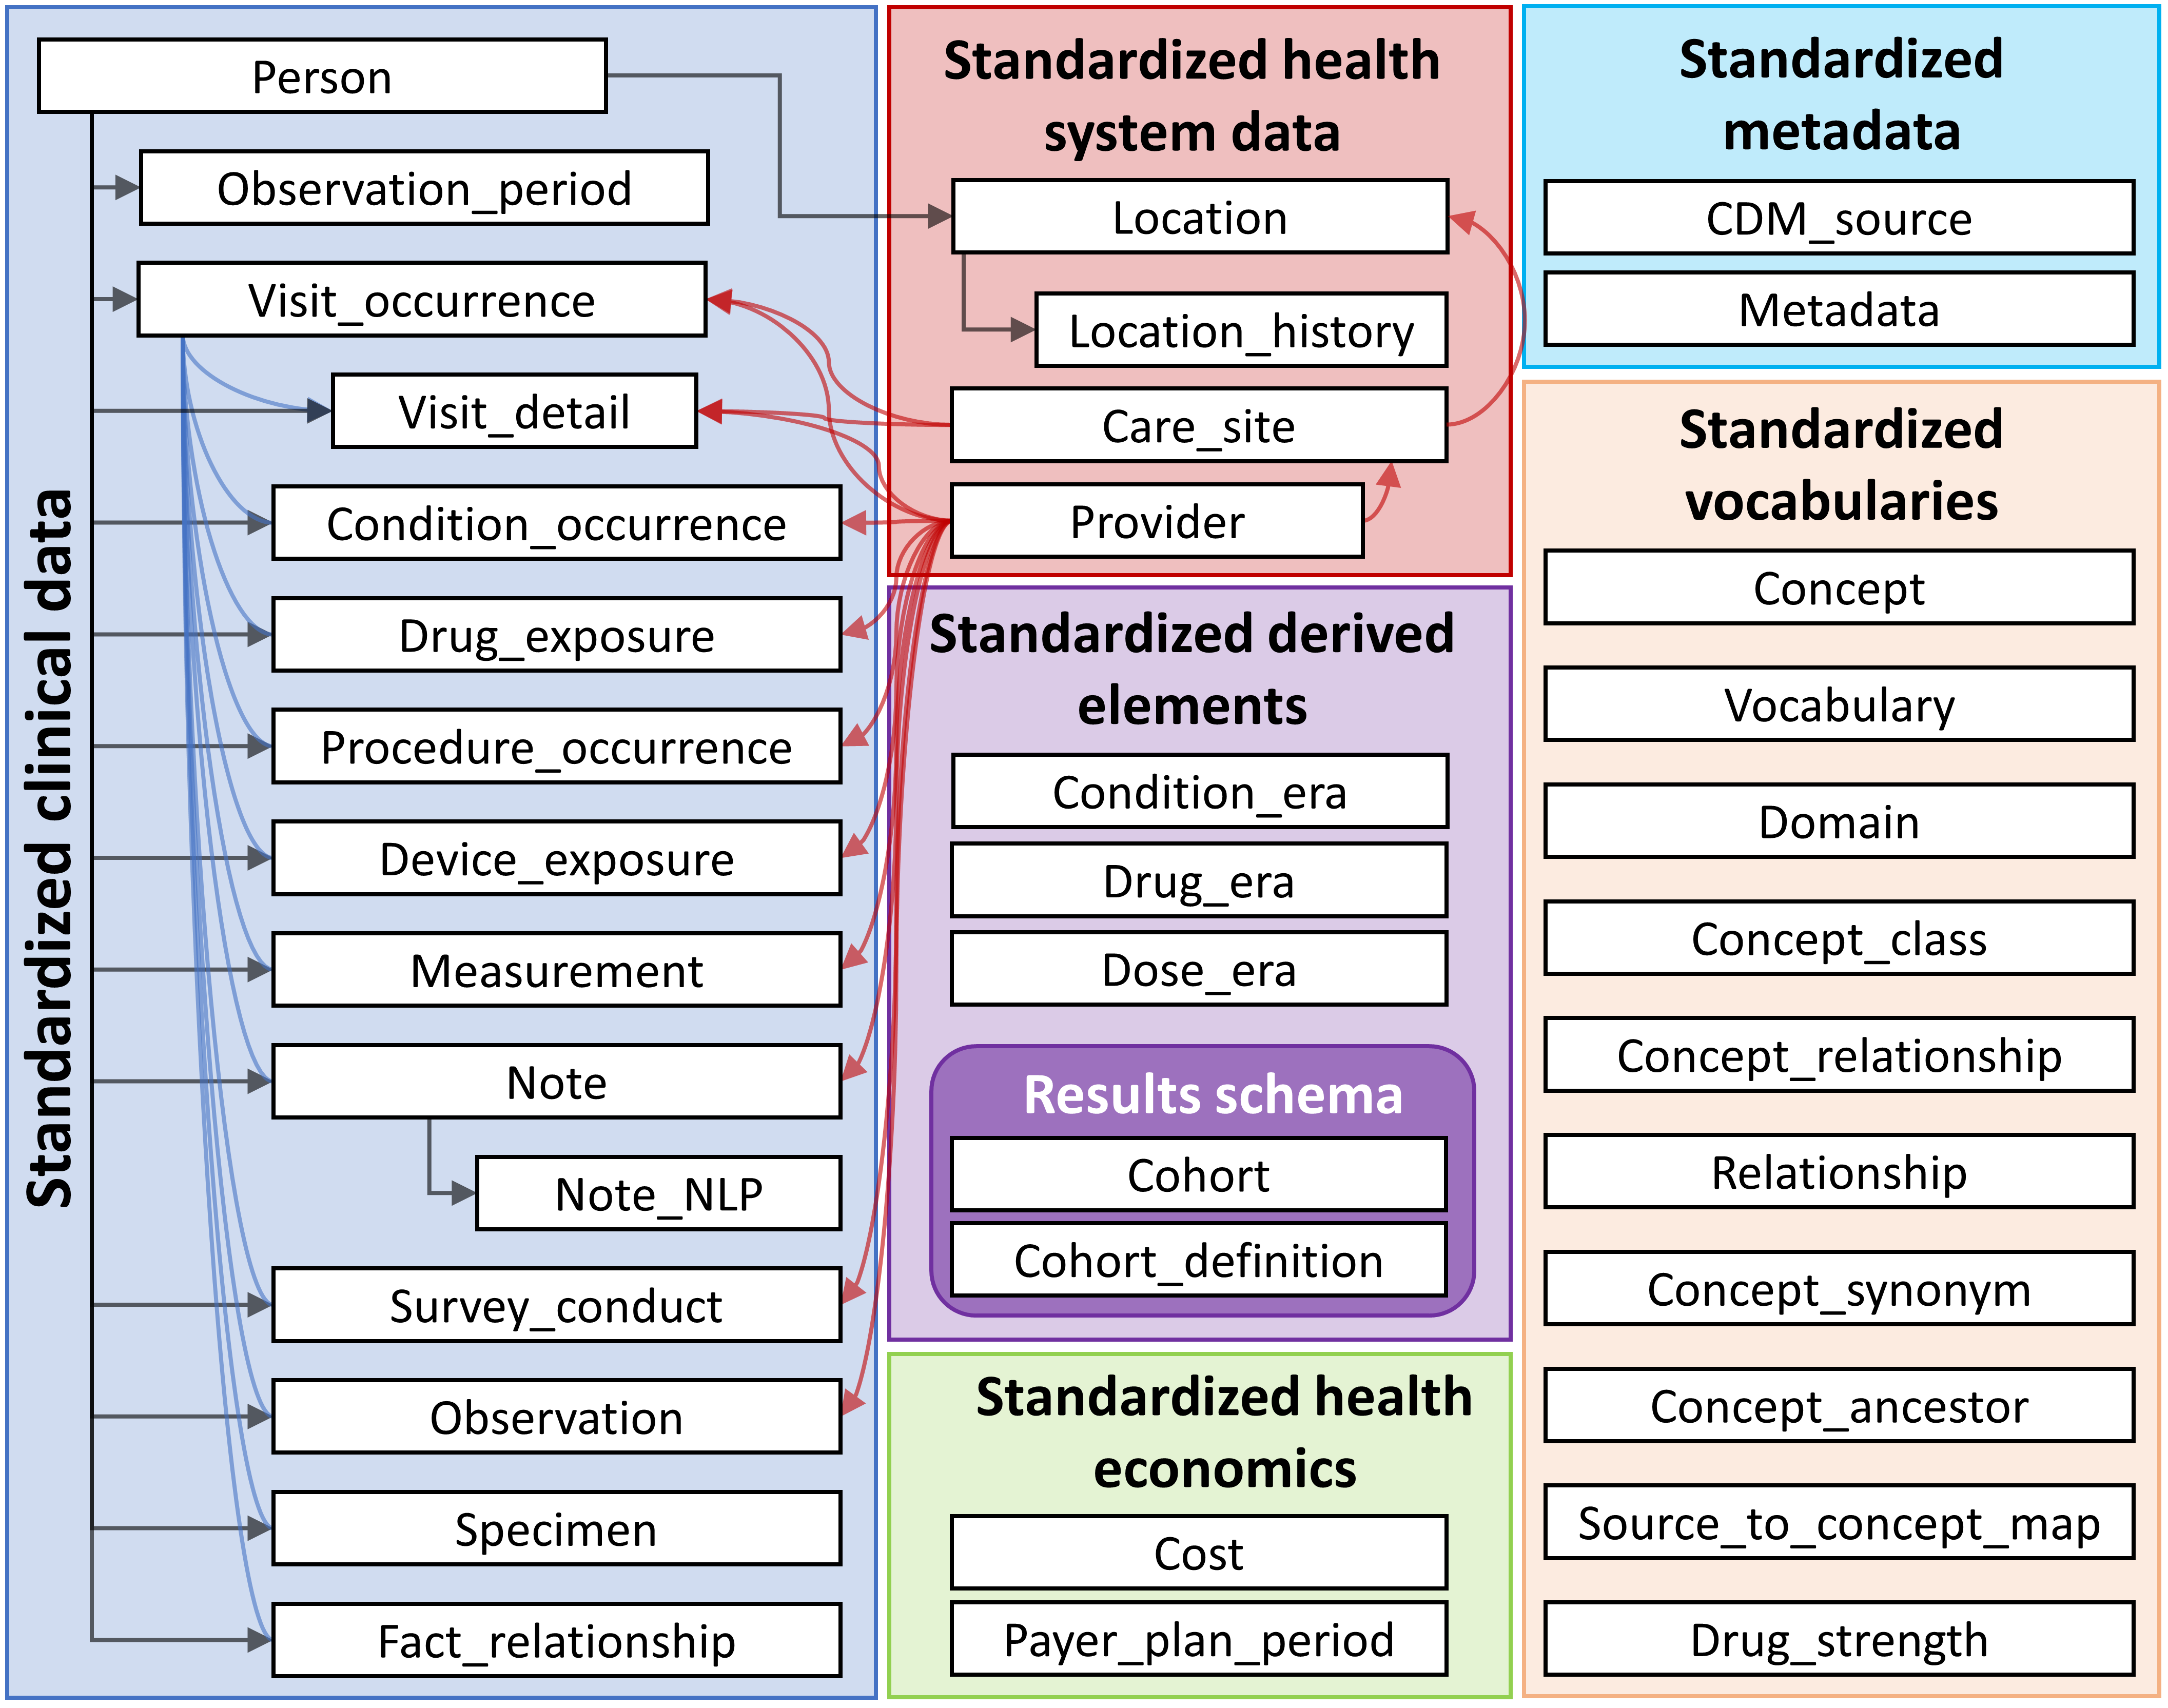
\includegraphics[width=1\linewidth]{images/CommonDataModel/cdmDiagram} \caption{CDMバージョン6.0のすべてのテーブルの概要。テーブル間のすべての関係が示されているわけではありません。}\label{fig:cdmDiagram}
\end{figure}

\section{デザインの原則}\label{ux30c7ux30b6ux30a4ux30f3ux306eux539fux5247}

CDMは、以下の目的のために最適化されています。 \index{Common Data Model!デザインの原則}

\begin{itemize}
\tightlist
\item
  特定の医療介入(薬物曝露、処置、医療政策の変更など)やアウトカム(コンディション、処置、他の薬物曝露など)を持つ患者集団を特定する。
\item
  人口統計情報、疾患の自然経過、医療提供、利用と費用、併存疾患、治療や治療の順序などさまざまなパラメータに関して患者集団の特性を評価する。
\item
  個々の患者でアウトカムが発生する可能性を予測する―― 第 \ref{PatientLevelPrediction} 章参照。
\item
  これらの介入が集団に及ぼす影響を推定する ―― 第 \ref{PopulationLevelEstimation} 章参照。
\end{itemize}

この目標を達成するために、CDMの開発は以下のデザイン要素に従います:

\begin{itemize}
\tightlist
\item
  \textbf{目的適合性}: CDMは、医療提供者または保険者の運用ニーズを満たす目的ではなく、分析のために最適な形でデータを提供することを目指しています。 \index{Common Data Model!目的適合性}
\item
  \textbf{データ保護}: 名前や正確な誕生日など、患者の身元や保護を危うくする可能性のあるすべてのデータは限定されています。乳児の研究のために正確な誕生日が必要な場合など、研究でより詳細な情報が明示的に必要な場合は例外となることがあります。 \index{Common Data Model!データ保護}
\item
  \textbf{ドメインの設計}: ドメインは、各レコードに最低限、個人の識別情報と日付が記録される、個人中心のリレーショナルデータモデルでモデル化されています。ここでいうリレーショナルデータモデルとは、主キーと外部キーでリンクされたテーブルの集合としてデータが表現されるものを指します。
\item
  \textbf{ドメインの根拠}: ドメインは、分析のユースケースがある場合(たとえばコンディション)で、そのドメインが他のものには適用されない特定の属性を持つ場合に、エンティティ-リレーションシップモデルで特定され、個別に定義されます。他のデータはすべて、エンティティ-属性-値構造の観察テーブルに保持できます。 \index{Common Data Model!ドメイン}
\item
  \textbf{標準化されたボキャブラリ}: それらの記録の内容を標準化するために、CDMは、標準的な医療コンセプトのすべてに対応する、必要かつ適切な標準化されたボキャブラリに依存しています。。
\item
  \textbf{既存のボキャブラリの再利用}: 可能な場合、国立医学図書館、退役軍人省、疾病予防管理センターなどの国立または業界の標準化やボキャブラリ定義を行う組織やイニシアティブはこれらのコンセプトを活用しています。
\item
  \textbf{ソースコードの保持}: すべてのコードが標準化されたボキャブラリにマッピングされている場合でも、モデルは元のソースコードも保持して、情報が失われないようにしています。 \index{Common Data Model!ソースコード} \index{Common Data Model!データ損失防止}
\item
  \textbf{技術の中立性}: CDMは特定のテクノロジーを必要としません。Oracle、SQL Serverなどのあらゆるリレーショナルデータベース、またはSAS分析データセットとして実現できます。 \index{Common Data Model!技術の中立性}
\item
  \textbf{スケーラビリティ}: CDMは、データベースに含まれる何億人もの人々や何十億件もの臨床観察データなど、さまざまな規模のデータソースに対応できるよう、データ処理と計算分析用に最適化されています。 \index{Common Data Model!スケーラビリティ}
\item
  \textbf{後方互換性}: これまでのCDMからの変更はすべてgithubリポジトリ\href{https://github.com/OHDSI/CommonDataModel}{(https://github.com/OHDSI/CommonDataModel)}で明確に示されています。CDMの旧バージョンは現在のバージョンから簡単に作成でき、以前に存在していた情報が失われることはありません。 \index{Common Data Model!後方互換性}
\end{itemize}

\section{データモデルの規約}\label{ux30c7ux30fcux30bfux30e2ux30c7ux30ebux306eux898fux7d04}

CDMでは、暗黙的および明示的な規約が数多く採用されています。CDMに対応するメソッドの開発者は、これらの規約を理解する必要があります。\index{共通データモデル!規約}

\subsection{モデルの一般的な規約}\label{model-Conv}

CDMは「人中心」のモデルと見なされており、すべての臨床イベントのテーブルがPERSONテーブルにリンクされています。日付または開始日と組み合わせることで、人ごとに医療関連イベントをすべて縦断的に見ることができます。このルールに対する例外は、標準化された医療システム・データ・テーブルで、これはさまざまなドメインのイベントに直接リンクされています。

\subsection{スキーマの一般的な規約}\label{ux30b9ux30adux30fcux30deux306eux4e00ux822cux7684ux306aux898fux7d04}

スキーマ(または一部のシステムではデータベースユーザー)により、読み取り専用テーブルと読み取り/書き込みテーブルを分離することができます。臨床イベントやボキャブラリテーブルは「CDM」スキーマにあり、エンドユーザーや分析ツールからは読み取り専用と見なされます。ウェブベースのツールやエンドユーザーが操作する必要のあるテーブルは、「Results」スキーマに格納されます。「Results」スキーマの2つのテーブルは、COHORTとCOHORT\_DEFINITIONです。これらのテーブルは、ユーザーが定義する可能性のあるグループを記述することを目的としています。詳細は第 \ref{Cohorts}章を参照ください。これらのテーブルは書き込み可能であり、実行時にCOHORTテーブルにコホートを保存することができます。すべてのユーザーに対して読み取り/書き込み可能なスキーマは1つだけなので、複数のユーザーアクセスをどのように構成し制御するかは、CDMの実装次第です。

\subsection{データテーブルの一般的な規約}\label{ux30c7ux30fcux30bfux30c6ux30fcux30d6ux30ebux306eux4e00ux822cux7684ux306aux898fux7d04}

CDMはプラットフォームに依存しません。データ型はANSI SQLデータ型(VARCHAR、INTEGER、FLOAT、DATE、DATETIME、CLOB)を用いて一般的に定義されます。VARCHARには最小必要文字列長のみが指定され、具体的なCDMのインスタンス内で拡張できます。CDMは日付および日時の形式を規定しません。CDMに対する標準クエリは、ローカルインスタンスや日付/日時の設定によって異なる場合があります。

\textless\textless\textless\textless\textless\textless\textless{} HEAD
\emph{注意}: データモデル自体はプラットフォームに依存しませんが、それに対応するために構築された多くのツールは特定の仕様が必要です。詳細については、第 \ref{OhdsiAnalyticsTools}章をご覧ください。

\subsection{ドメインの一般的な規約}\label{domains}

異なる性質のイベントはドメインに整理されています。これらのイベントはドメイン固有のテーブルやフィールドに格納され、標準化されたボキャブラリで定義されたドメイン固有の標準コンセプトによって表現されます(第 \ref{conceptDomains}部参照)。 各標準コンセプトには一意のドメイン割り当てがあり、どのテーブルに記録されるかを定義します。正しいドメイン割り当てはコミュニティ内で議論の余地がありますが、この厳格なドメインテーブルフィールドの対応規則により、コードやコンセプトの記録場所が常に明確であることが保証されます。例えば、徴候、症状、診断のコンセプトはコンディション・ドメインに属し、CONDITION\_OCCURRENCEテーブルのCONDITION\_CONCEPT\_IDに記録されます。処置薬と呼ばれるものは通常、ソースデータの処置テーブルに処置コードとして記録されます。CDMでは、対応する標準コンセプトにドメイン割り当て「Drug」が設定されているため、これらのレコードはDRUG\_EXPOSUREテーブルに記録されます。ドメインの総数は30で、表\ref{tab:domains}に示されています。

表: \label{tab:domains} 各ドメインに属する標準コンセプトの数。

\begin{longtable}[]{@{}
  >{\raggedright\arraybackslash}p{(\columnwidth - 6\tabcolsep) * \real{0.2029}}
  >{\raggedright\arraybackslash}p{(\columnwidth - 6\tabcolsep) * \real{0.2899}}
  >{\raggedright\arraybackslash}p{(\columnwidth - 6\tabcolsep) * \real{0.2029}}
  >{\raggedright\arraybackslash}p{(\columnwidth - 6\tabcolsep) * \real{0.3043}}@{}}
\caption{\label{tab:domains} 各ドメインに属する標準コンセプトの数}\tabularnewline
\toprule\noalign{}
\begin{minipage}[b]{\linewidth}\raggedright
コンセプト数
\end{minipage} & \begin{minipage}[b]{\linewidth}\raggedright
ドメインID
\end{minipage} & \begin{minipage}[b]{\linewidth}\raggedright
コンセプト数
\end{minipage} & \begin{minipage}[b]{\linewidth}\raggedright
ドメインID
\end{minipage} \\
\midrule\noalign{}
\endfirsthead
\toprule\noalign{}
\begin{minipage}[b]{\linewidth}\raggedright
コンセプト数
\end{minipage} & \begin{minipage}[b]{\linewidth}\raggedright
ドメインID
\end{minipage} & \begin{minipage}[b]{\linewidth}\raggedright
コンセプト数
\end{minipage} & \begin{minipage}[b]{\linewidth}\raggedright
ドメインID
\end{minipage} \\
\midrule\noalign{}
\endhead
\bottomrule\noalign{}
\endlastfoot
1731378 & Drug & 183 & Route \\
477597 & Device & 180 & Currency \\
257000 & Procedure & 158 & Payer \\
163807 & Condition & 123 & Visit \\
145898 & Observation & 51 & Cost \\
89645 & Measurement & 50 & Race \\
33759 & Spec Anatomic Site & 13 & Plan Stop Reason \\
17302 & Meas Value & 11 & Plan \\
1799 & Specimen & 6 & Episode \\
1215 & Provider Specialty & 6 & Sponsor \\
1046 & Unit & 5 & Meas Value Operator \\
944 & Metadata & 3 & Spec Disease Status \\
538 & Revenue Code & 2 & Gender \\
336 & Type Concept & 2 & Ethnicity \\
194 & Relationship & 1 & Observation Type \\
\end{longtable}

\subsection{コンテンツのコンセプトによる表現}\label{ux30b3ux30f3ux30c6ux30f3ux30c4ux306eux30b3ux30f3ux30bbux30d7ux30c8ux306bux3088ux308bux8868ux73fe}

CDMデータテーブル内の各レコードのコンテンツは完全に正規化され、コンセプトを通じて表現されます。コンセプトはCONCEPTテーブルへの外部キーであるCONCEPT\_ID値とともにイベントテーブルに格納され、CONCEPTテーブルは一般的な参照テーブルとして機能します。CDMインスタンスはすべて、コンセプトの参照として同じCONCEPTテーブルを使用します。これにより、CDMとともにOHDSI研究ネットワークの基盤となる相互運用性の主要なメカニズムが提供されます。標準コンセプトが存在しない場合や特定できない場合、CONCEPT\_IDの値は0に設定されます。これは、存在しないコンセプト、不明またはマッピング不可能な値を表します。

CONCEPTテーブルのレコードには、各コンセプトの詳細情報(名前、ドメイン、クラスなど)が含まれています。コンセプト、コンセプトリレーションシップ、コンセプトの祖先など、コンセプトに関連するその他の情報は、標準化されたボキャブラリのテーブルに含まれています(第 \ref{StandardizedVocabularies}章を参照)。

\subsection{フィールドの一般的な命名規約}\label{ux30d5ux30a3ux30fcux30ebux30c9ux306eux4e00ux822cux7684ux306aux547dux540dux898fux7d04}

すべてのテーブルの変数名は1つの規約に従います。

\begin{longtable}[]{@{}
  >{\raggedright\arraybackslash}p{(\columnwidth - 2\tabcolsep) * \real{0.5000}}
  >{\raggedright\arraybackslash}p{(\columnwidth - 2\tabcolsep) * \real{0.5000}}@{}}
\caption{\label{tab:fieldConventions} フィールド名の規約}\tabularnewline
\toprule\noalign{}
\begin{minipage}[b]{\linewidth}\raggedright
記法
\end{minipage} & \begin{minipage}[b]{\linewidth}\raggedright
説明
\end{minipage} \\
\midrule\noalign{}
\endfirsthead
\toprule\noalign{}
\begin{minipage}[b]{\linewidth}\raggedright
記法
\end{minipage} & \begin{minipage}[b]{\linewidth}\raggedright
説明
\end{minipage} \\
\midrule\noalign{}
\endhead
\bottomrule\noalign{}
\endlastfoot
{[}Event{]}\_ID & 各レコードの固有の識別子で、イベントテーブル間の関係を確立する外部キーとして機能します。例えば、PERSON\_IDは各個人を一意に識別します。VISIT\_OCCURRENCE\_IDは受診期間を一意に識別します。 \\
{[}Event{]}\_CONCEPT\_ID & CONCEPT参照テーブルの標準コンセプトレコードへの外部キーです。これはイベントの主要な表現として機能し、標準化された分析の主要な基礎となります。たとえば、CONDITION\_CONCEPT\_ID = \href{http://athena.ohdsi.org/search-terms/terms/31967}{31967}にはSNOMEDコンセプトの「吐き気」の参照値が含まれています。 \\
{[}Event{]}\_SOURCE\_CONCEPT\_ID & CONCEPT参照テーブルのレコードへの外部キーです。このコンセプトは、以下のソース値に相当し、標準コンセプトの場合、それは{[}Event{]}\_CONCEPT\_IDと同一になります。例えば、CONDITION\_SOURCE\_CONCEPT\_ID = \href{http://athena.ohdsi.org/search-terms/terms/45431665}{45431665}は「吐き気」というコンセプトを、Read用語で示し、同様のCONDITION\_CONCEPT\_IDは標準のSNOMED-CTコンセプト\href{http://athena.ohdsi.org/search-terms/terms/31967}{31967}です。標準分析アプリケーションの場合、ソースコンセプトの使用は推奨されません。なぜなら、標準コンセプトだけがイベントの意味的内容を明確に示し、ソースコンセプトは相互運用可能ではないためです。 \\
{[}Event{]}\_TYPE\_CONCEPT\_ID & ソース情報の出所を示す標準化されたボキャブラリ内で標準化されたコンセプト参照テーブルのレコードへの外部キーです。フィールド名とは異なり、これはイベントの種類やコンセプトの種類でもなく、このレコードを作成した取得メカニズムを宣言するものであることに留意ください。例として、DRUG\_TYPE\_CONCEPT\_IDは、薬剤レコードが薬局での調剤イベント(「薬局での調剤」)から派生したものか、処方アプリケーション(「処方箋発行」)から派生したものかを区別します。 \\
{[}Event{]}\_SOURCE\_VALUE & ソースデータでこのイベントがどのように表現されていたかを反映する、逐語的なコードまたは自由形式の文字列。これらのソース値はデータソース間で整合されていないため、標準的な分析アプリケーションでの使用は推奨されません。例えば、CONDITION\_SOURCE\_VALUEにはドットを省略した表記で書かれたICD-9コード787.02に対応する「78702」のレコードが含まれる可能性があります。 \\
\end{longtable}

\subsection{コンセプトとソース値の違い}\label{concepts-Sources}

多くのテーブルには、ソース値、ソースコンセプト、標準コンセプトとして、複数の場所に同等の情報が含まれています。

\begin{itemize}
\tightlist
\item
  \textbf{ソース値}は、ソースデータにおけるイベントレコードのオリジナル表現です。これらは、ICD9CM、NDC、Readなどのように、広く使用されているがパブリックドメインであることが多いコーディングシステムからのコード、CPT4、GPI、MedDRAなどの独自のコーディングシステム、あるいは女性をF、男性をMのようにソースデータのみで使用される管理された用語集であることがあります。また、標準化も管理もされていない短い自由テキストのフレーズであることもあります。ソース値は、データテーブルの{[}Event{]}\_SOURCE\_VALUEフィールドに格納されます。
\item
  \textbf{コンセプト}は、CDM特有のエンティティであり、臨床事実の意味を標準化します。ほとんどのコンセプトは、医療分野における既存の公開または独自仕様のコーディングシステムに基づきますが、中には新規に作成されたものもあります(CONCEPT\_CODEが「OMOP」で始まる)。コンセプトには、すべてのドメインにわたって一意のIDが割り当てられています。
\item
  \textbf{ソースコンセプト}は、ソースで使用されるコードを表すコンセプトです。ソースコンセプトは、既存の公開または独自のコード体系に対してのみ使用され、OMOPで生成されたコンセプトには使用されません。ソースコンセプトはデータテーブル内の{[}Event{]}\_SOURCE\_CONCEPT\_IDフィールドに格納されます。
\item
  \textbf{標準コンセプト}は、ソースで使用されるコードシステムとは無関係に、すべてのデータベースで臨床実態の意味を一意に定義するために使用されるコンセプトです。標準コンセプトは通常、既存の公開または専有のボキャブラリソースから取得されます。標準コンセプトと同等な意味を持つ非標準コンセプトは、標準化されたボキャブラリにおいて標準コンセプトにマッピングされます。標準コンセプトはデータテーブルの{[}Event{]}\_CONCEPT\_IDフィールドで参照できます。
\end{itemize}

ソース値は、便宜上、品質保証(QA)の目的でのみ提供されます。ソース値には、特定のデータソースの文脈のみで意味を持つ情報が含まれる場合があります。ソース値やソースコンセプトの使用は任意ですが、ソースデータがコード体系を使用している場合には\textbf{強く推奨}されます。一方、標準コンセプトの使用は\textbf{必須}です。この標準コンセプトの使用が必須である理由は、すべてのCDMインスタンスが同じ言語を話すことができるようにするためです。例えば、図 \ref{fig:pulmTubICD9} で示されているように、コンディション「肺結核」(TB)のICD9CMコードは011です。

\begin{figure}

{\centering 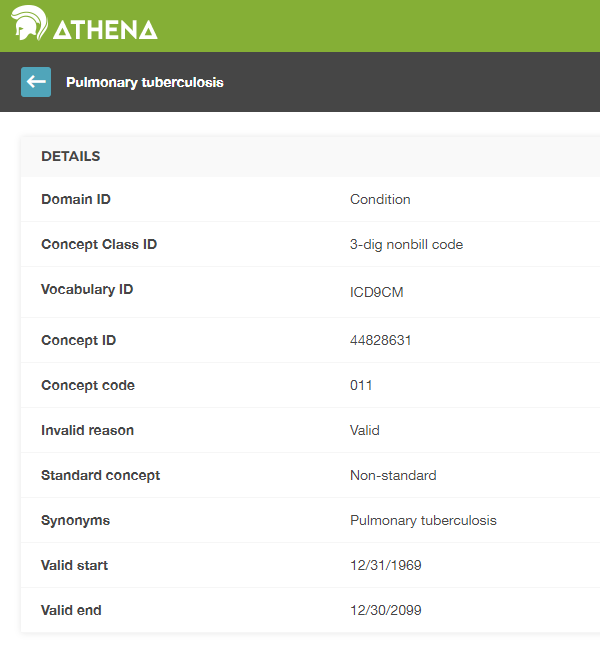
\includegraphics[width=0.75\linewidth]{images/CommonDataModel/pulmTubICD9} 

}

\caption{肺結核のICD9CMコード}\label{fig:pulmTubICD9}
\end{figure}

文脈がなければ、コード011は、UB04ボキャブラリでは「病院入院患者(メディケアパートAを含む)」、DRGボキャブラリでは「神経系新生物(合併症、併発症なし)」と解釈される可能性があります。 このような場合に、ソースと標準の両方のコンセプトIDが役立ちます。ICD9CMの011を表すCONCEPT\_IDの値は\href{http://athena.ohdsi.org/search-terms/terms/44828631}{44828631}です。これにより、UBO4とDRGとICD9CMが区別されます。ICD9CM TB のソースコンセプト は、図 \ref{fig:pulmTubMap} に示されているように、「非標準から標準へのマップ(OMOP)」という関係を通じて、SNOMED ボキャブラリーから Standard Concept \href{http://athena.ohdsi.org/search-terms/terms/253954}{253954}にマップされます。この同じマッピング関係は、Read、ICD10、CIEL、MeSH コードなどにも存在するため、SNOMED 標準コンセプトを参照するあらゆる検索は、サポートされているすべてのソースコードを含みます。

\begin{figure}
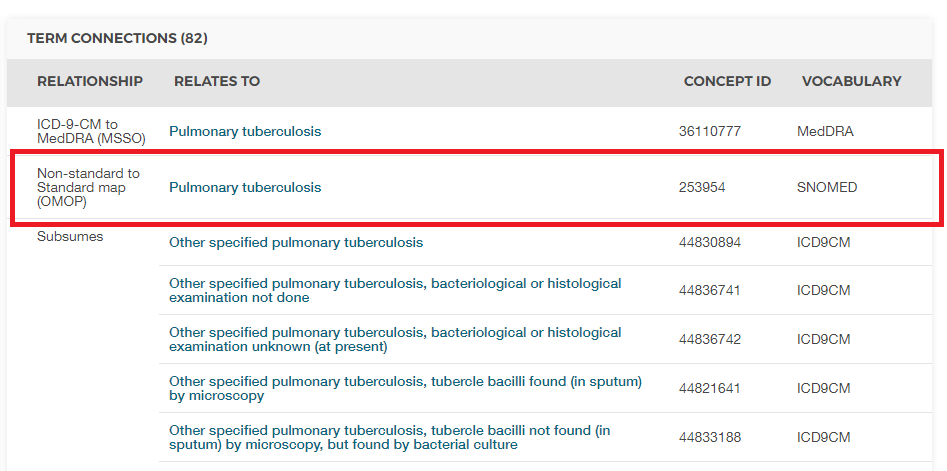
\includegraphics[width=1\linewidth]{images/CommonDataModel/pulmTubMap} \caption{肺結核のSNOMEDコード}\label{fig:pulmTubMap}
\end{figure}

標準コンセプトとソースコンセプトとの関係の例を表 \ref{tab:conditionOccurrence}に示します。

\section{CDM標準化テーブル}\label{cdmux6a19ux6e96ux5316ux30c6ux30fcux30d6ux30eb}

\index{共通データモデル!標準化テーブル}

CDMには16の臨床イベントテーブル、10のボキャブラリテーブル、2つのメタデータテーブル、4つのヘルスシステムデータテーブル、2つの医療経済データテーブル、3つの標準化された派生要素、および2つの結果スキーマテーブルが含まれています。 これらのテーブルはCDM Wikiで完全に指定されています \footnote{\url{https://github.com/OHDSI/CommonDataModel/wiki}}。

これらのテーブルが実際にどのように使用されるかを説明するために、本章の残りの部分ではある1人のデータを一貫した例として使用します。

\subsection{実行例: 子宮内膜症}\label{ux5b9fux884cux4f8b-ux5b50ux5baeux5185ux819cux75c7}

子宮内膜症は、通常女性の子宮内膜にある細胞が体の他の場所に生じる痛みを伴う状態です。重症になると、不妊症、腸や膀胱の問題を引き起こすことがあります。次のセクションでは、この病気にかかった患者の経験と、それが共通データモデルでどのように表現される可能性があるかを詳しく説明します。

\begin{center}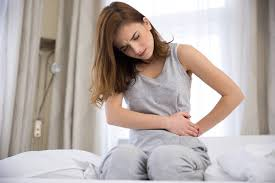
\includegraphics[width=0.5\linewidth]{images/CommonDataModel/Lauren} \end{center}

\begin{quote}
この痛みを伴う旅のすべての段階で、どれほど痛みを感じているかを皆に納得させなければなりませんでした。
\end{quote}

Laurenは何年も子宮内膜症の症状に悩まされてきましたが、診断を受けるまでには卵巣嚢腫の破裂を経験しています。Laurenについての詳細は\url{https://endometriosis-uk.org/laurens-story} をご覧ください。

\subsection{PERSONテーブル}\label{person}

\subsubsection*{Laurenについてわかっていること}\label{laurenux306bux3064ux3044ux3066ux308fux304bux3063ux3066ux3044ux308bux3053ux3068}
\addcontentsline{toc}{subsubsection}{Laurenについてわかっていること}

\begin{itemize}
\tightlist
\item
  彼女は36歳の女性です
\item
  彼女の誕生日は1982年3月12日です
\item
  彼女は白人です
\item
  彼女はイギリス人です
\end{itemize}

これを踏まえると、彼女のPERSONテーブルは次のようになります:

\begin{longtable}[]{@{}
  >{\raggedright\arraybackslash}p{(\columnwidth - 4\tabcolsep) * \real{0.3333}}
  >{\raggedright\arraybackslash}p{(\columnwidth - 4\tabcolsep) * \real{0.3333}}
  >{\raggedright\arraybackslash}p{(\columnwidth - 4\tabcolsep) * \real{0.3333}}@{}}
\caption{\label{tab:person} PERSONテーブル}\tabularnewline
\toprule\noalign{}
\begin{minipage}[b]{\linewidth}\raggedright
列名
\end{minipage} & \begin{minipage}[b]{\linewidth}\raggedright
値
\end{minipage} & \begin{minipage}[b]{\linewidth}\raggedright
説明
\end{minipage} \\
\midrule\noalign{}
\endfirsthead
\toprule\noalign{}
\begin{minipage}[b]{\linewidth}\raggedright
列名
\end{minipage} & \begin{minipage}[b]{\linewidth}\raggedright
値
\end{minipage} & \begin{minipage}[b]{\linewidth}\raggedright
説明
\end{minipage} \\
\midrule\noalign{}
\endhead
\bottomrule\noalign{}
\endlastfoot
PERSON\_ID & 1 & PERSON\_IDはソースから直接であれ、ビルドプロセスの一部として生成されたものであれ、整数である必要があります。 \\
GENDER\_CONCEPT\_ID & 8532 & 女性性別を参照するコンセプトIDは\href{http://athena.ohdsi.org/search-terms/terms/8532}{8532}です。 \\
YEAR\_OF\_BIRTH & 1982 & \\
MONTH\_OF\_BIRTH & 3 & \\
DAY\_OF\_BIRTH & 12 & \\
BIRTH\_DATETIME & 1982-03-12 00:00:00 & 時間が不明の場合は真夜中が使用されます。 \\
DEATH\_DATETIME & & \\
RACE\_CONCEPT\_ID & 8527 & 白人を示すコンセプトIDは\href{http://athena.ohdsi.org/search-terms/terms/8527}{8527}です。英国の民族は\href{http://athena.ohdsi.org/search-terms/terms/4093769}{4093769}です。どちらも正しいですが、後者は前者に統合されます。民族は、ETHNICITY\_CONCEPT\_IDではなく、人種の一部としてここに格納されていることに留意ください。 \\
ETHNICITY\_CONCEPT\_ ID & 38003564 & これはヒスパニック系の人々を他の人々から区別するための米国特有の表記法です。この場合の「English」という民族性は、RACE\_CONCEPT\_ID に格納されます。米国以外では使用されません。\href{http://athena.ohdsi.org/search-terms/terms/38003564}{38003564}は「ヒスパニックではない」を表します。 \\
LOCATION\_ID & & 彼女の住所は不明です。 \\
PROVIDER\_ID & & 彼女のプライマリケア提供者は不明です。 \\
CARE\_SITE & & 彼女の主な医療施設は不明です。 \\
PERSON\_SOURCE\_ VALUE & 1 & 通常、これはソースデータでの彼女の識別子ですが、多くの場合、それはPERSON\_IDと同じです。 \\
GENDER\_SOURCE\_ VALUE & F & ソースに表示されている性別値がここに格納されています。 \\
GENDER\_SOURCE\_ CONCEPT\_ID & 0 & ソースの性別値が OHDSI がサポートするコーディングスキームでコード化されている場合、そのコンセプトはここに格納されます。例えば、ソースの性別が「性別-F」であり、PCORNet ボキャブラリコンセプトに記載されている場合、\href{http://athena.ohdsi.org/search-terms/terms/44814665}{44814665}がこのフィールドに入ります。 \\
RACE\_SOURCE\_ VALUE & white & ソースに表示されてい人種値がここに格納されます。 \\
RACE\_SOURCE\_ CONCEPT\_ID & 0 & 同様にGENDER\_SOURCE\_CONCEPT\_IDの原則が適用されます。 \\
ETHNICITY\_SOURCE\_ VALUE & english & ソースに表示されている民族値がここに格納されます。 \\
ETHNICITY\_SOURCE\_ CONCEPT\_ID & 0 & 同様にGENDER\_SOURCE\_CONCEPT\_IDの原則が適用されます。 \\
\end{longtable}

\subsection{OBSERVATION\_PERIODテーブル}\label{observationPeriod}

OBSERVATION\_PERIODテーブルは、妥当な感度と特異度が期待されるソースシステムにおいて、少なくとも患者の人口統計、コンディション、処置、薬剤が記録される期間を定義するために設計されています。保険請求データの場合は、通常、患者の加入期間となります。電子健康記録(EHR)の場合は、より複雑です。ほとんどの医療システムでは、どの医療機関または医療提供者が訪問したかを特定しないためです。次善の策として、システム内の最初のレコードが観察期間の開始日と見なされ、最新のレコードが終了日と見なされることがよくあります。

\subsubsection*{Laurenの観察期間はどのように定義されているのですか?}\label{laurenux306eux89b3ux5bdfux671fux9593ux306fux3069ux306eux3088ux3046ux306bux5b9aux7fa9ux3055ux308cux3066ux3044ux308bux306eux3067ux3059ux304b}
\addcontentsline{toc}{subsubsection}{Laurenの観察期間はどのように定義されているのですか?}

Laurenの情報が表 \ref{tab:encounters}に示されているように電子健康記録システムに記録されているとしましょう。彼女の観察期間の元となる彼女の受診は:

\begin{longtable}[]{@{}llll@{}}
\caption{\label{tab:encounters} Laurenのヘルスケアエンカウンター}\tabularnewline
\toprule\noalign{}
エンカウンターID & 開始日 & 終了日 & タイプ \\
\midrule\noalign{}
\endfirsthead
\toprule\noalign{}
エンカウンターID & 開始日 & 終了日 & タイプ \\
\midrule\noalign{}
\endhead
\bottomrule\noalign{}
\endlastfoot
70 & 2010-01-06 & 2010-01-06 & 外来患者 \\
80 & 2011-01-06 & 2011-01-06 & 外来患者 \\
90 & 2012-01-06 & 2012-01-06 & 外来患者 \\
100 & 2013-01-07 & 2013-01-07 & 外来患者 \\
101 & 2013-01-14 & 2013-01-14 & 歩行可能 \\
102 & 2013-01-17 & 2013-01-24 & 入院患者 \\
\end{longtable}

エンカウンターレコードに基づいて彼女のOBSERVATION\_PERIODテーブルは次のようになるかもしれません:

\begin{longtable}[]{@{}
  >{\raggedright\arraybackslash}p{(\columnwidth - 4\tabcolsep) * \real{0.3333}}
  >{\raggedright\arraybackslash}p{(\columnwidth - 4\tabcolsep) * \real{0.3333}}
  >{\raggedright\arraybackslash}p{(\columnwidth - 4\tabcolsep) * \real{0.3333}}@{}}
\caption{\label{tab:observationPeriod} OBSERVATION\_PERIODテーブル}\tabularnewline
\toprule\noalign{}
\begin{minipage}[b]{\linewidth}\raggedright
列名
\end{minipage} & \begin{minipage}[b]{\linewidth}\raggedright
値
\end{minipage} & \begin{minipage}[b]{\linewidth}\raggedright
説明
\end{minipage} \\
\midrule\noalign{}
\endfirsthead
\toprule\noalign{}
\begin{minipage}[b]{\linewidth}\raggedright
列名
\end{minipage} & \begin{minipage}[b]{\linewidth}\raggedright
値
\end{minipage} & \begin{minipage}[b]{\linewidth}\raggedright
説明
\end{minipage} \\
\midrule\noalign{}
\endhead
\bottomrule\noalign{}
\endlastfoot
OBSERVATION\_ PERIOD\_ID & 1 & これは通常、自動生成された値で、テーブル内の各レコードに一意の識別子を生成します。 \\
PERSON\_ID & 1 & これはPERSONテーブルでLauraのレコードへの外部キーであり、PERSONをOBSERVATION\_PERIODテーブルにリンクします。 \\
OBSERVATION\_PERIOD\_ START\_DATE & 2010-01-06 & これは記録上、彼女の最初のエンカウンターの開始日です。 \\
OBSERVATION\_PERIOD\_ END\_DATE & 2013-01-24 & これは記録上、彼女の最後のエンカウンターの終了日です。 \\
PERIOD\_TYPE\_ CONCEPT\_ID & 44814725 & 「Obs Period Type」コンセプトクラスを持つボキャブラリにおける最良のオプションは\href{http://athena.ohdsi.org/search-terms/terms/44814724}{44814724}で、「ヘルスケアエンカウンターをカバーする期間」を表します。 \\
\end{longtable}

\subsection{VISIT\_OCCURRENCE}\label{visitOccurrence}

VISIT\_OCCURRENCEテーブルには、患者が医療システムを利用した際の情報が格納されています。OHDSIでは、これらの情報を「訪問」と呼び、個別のイベントとして扱います。訪問には12のトップカテゴリーがあり、医療が提供されるさまざまな状況を描写する広範な階層構造があります。最も多く記録されている受診は、入院、外来、救急外来、医療機関以外の施設へのビジットです。

\subsubsection*{Laurenのエンカウンターが受診期間としてどのように表現されるか?}\label{laurenux306eux30a8ux30f3ux30abux30a6ux30f3ux30bfux30fcux304cux53d7ux8a3aux671fux9593ux3068ux3057ux3066ux3069ux306eux3088ux3046ux306bux8868ux73feux3055ux308cux308bux304b}
\addcontentsline{toc}{subsubsection}{Laurenのエンカウンターが受診期間としてどのように表現されるか?}

例として、ビジットのエンカウンターをVISIT\_OCCURRENCEテーブルで表現しましょう。

\begin{longtable}[]{@{}
  >{\raggedright\arraybackslash}p{(\columnwidth - 4\tabcolsep) * \real{0.3333}}
  >{\raggedright\arraybackslash}p{(\columnwidth - 4\tabcolsep) * \real{0.3333}}
  >{\raggedright\arraybackslash}p{(\columnwidth - 4\tabcolsep) * \real{0.3333}}@{}}
\caption{\label{tab:visitOccurrence} VISIT\_OCCURRENCEテーブル。}\tabularnewline
\toprule\noalign{}
\begin{minipage}[b]{\linewidth}\raggedright
列名
\end{minipage} & \begin{minipage}[b]{\linewidth}\raggedright
値
\end{minipage} & \begin{minipage}[b]{\linewidth}\raggedright
説明
\end{minipage} \\
\midrule\noalign{}
\endfirsthead
\toprule\noalign{}
\begin{minipage}[b]{\linewidth}\raggedright
列名
\end{minipage} & \begin{minipage}[b]{\linewidth}\raggedright
値
\end{minipage} & \begin{minipage}[b]{\linewidth}\raggedright
説明
\end{minipage} \\
\midrule\noalign{}
\endhead
\bottomrule\noalign{}
\endlastfoot
VISIT\_OCCURRENCE\_ID & 514 & これは通常、自動生成された値で、各レコードに一意の識別子を生成します。 \\
PERSON\_ID & 1 & これはPERSONテーブルでLaurenのレコードにリンクする外部キーです。 \\
VISIT\_CONCEPT\_ID & 9201 & 入院ビジットを参照するキーは\href{http://athena.ohdsi.org/search-terms/terms/9201}{9201}です。 \\
VISIT\_START\_DATE & 2013-01-17 & ビジットの開始日です。 \\
VISIT\_START\_ DATETIME & 2013-01-17 00:00:00 & ビジットの日付と時間です。時間が不明なため、深夜が使用されます。 \\
VISIT\_END\_DATE & 2013-01-24 & ビジットの終了日です。これは1日のビジットである場合、終了日は開始日と一致します。 \\
VISIT\_END\_DATETIME & 2013-01-24 00:00:00 & ビジットの終了日と時間です。時間が不明なため、真夜中が使用されます。 \\
VISIT\_TYPE\_ CONCEPT\_ID & 32034 & ビジットレコードの出所を示します。保険請求、病院請求、EHR記録など。これらのエンカウンターがEHRレコードに似ている例として、\href{http://athena.ohdsi.org/search-terms/terms/32035}{32035}(「EHRエンカウンターレコードから派生したビジット」)のコンセプトIDが使用されています。 \\
PROVIDER\_ID & NULL & エンカウンターレコードに提供者が関連付けられている場合、その提供者のIDがこのフィールドに格納されます。これが提供者テーブルのPROVIDER\_IDフィールドの内容であるはずです。 \\
CARE\_SITE\_ID & NULL & エンカウンターレコードに関連するケアサイトがある場合、そのケアサイトのIDがこのフィールドに入ります。これがCARE\_SITEテーブルのCARE\_SITE\_IDであるはずです。 \\
VISIT\_SOURCE\_ VALUE & 入院 & ビジット値はソースでどのように表示されるかに基づいてここに格納されます。Laurenのデータにはそれがありません。 \\
VISIT\_SOURCE\_ CONCEPT\_ID & NULL & ビジット値は、ソースがOHDSIによって認識されているボキャブラリを使用してコーディングされている場合、ソースコードを表すコンセプトID値がここに表示されます。Laurenのデータにはこの値はありません。 \\
ADMITTED\_FROM\_ CONCEPT\_ID & NULL & 既知の場合、患者が入院した場所を表すコンセプトが表示されます。このコンセプトのドメインは「ビジット」であるべきです。例えば、患者が自宅から病院に入院した場合には、コンセプトID \href{http://athena.ohdsi.org/search-terms/terms/8536}{8536}「自宅」が含まれます。 \\
ADMITTED\_FROM\_ SOURCE\_CONCEPT\_ID & NULL & 患者が入院した元の場所を表すソース値が表示されます。上記の例では「自宅」です。 \\
DISCHARGE\_TO\_ CONCEPT\_ID & NULL & 既知の場合、患者が退院した先の場所を表すコンセプトが含まれます。このコンセプトのドメインは「ビジット」であるべきです。例えば、患者が介護付き生活施設に退院した場合、コンセプトID \href{http://athena.ohdsi.org/search-terms/terms/8615}{8615}「介護付き生活施設」となります。 \\
DISCHARGE\_TO\_ SOURCE\_VALUE & NULL & 患者が退院した場所を表すソース値が含まれます。上記の例では「介護付き生活施設」となります。 \\
PRECEDING\_VIS & NULL & 現在のビジットの直前のビジットを示します。ADMITTED\_FROM\_CONCEPT\_IDとは対照的に、ビジットコンセプトではなく、実際のビジット発生記録にリンクします。また、注意すべきは後続のビジットがないことです。ビジット発生記録は、このフィールドを通じてのみリンクされます。 \\
\end{longtable}

\begin{itemize}
\tightlist
\item
  患者は、入院患者の場合によくあるように、1回の来院中に複数の医療提供者とやりとりすることがあります。これらのやりとりは、VISIT\_DETAILテーブルに記録することができます。この章では深く掘り下げませんが、VISIT\_DETAILテーブルの詳細については、\href{https://github.com/OHDSI/CommonDataModel/wiki/VISIT_DETAIL}{CDM wiki}を参照ください。
\end{itemize}

\subsection{CONDITION\_OCCURRENCE}\label{conditionOccurrence}

CONDITION\_OCCURRENCEテーブルのレコードは、医療従事者によって観察された、または患者によって報告された、コンディションの診断、徴候、または症状です。

\subsubsection*{Laurenの状態は何ですか?}\label{laurenux306eux72b6ux614bux306fux4f55ux3067ux3059ux304b}
\addcontentsline{toc}{subsubsection}{Laurenの状態は何ですか?}

彼女の記録を再確認すると、次のように述べられています。:

\begin{quote}
約3年前、それまでにも痛かった生理痛がますますひどくなっていることに気づきました。直腸のすぐ近くに鋭い突き刺すような痛みを感じ、尾骨と骨盤下部のあたりが圧痛と腫れを伴っていることに気づきました。生理痛がひどくなり、月に1~2日は仕事を休むほどでした。鎮痛剤で痛みを和らげられることもありましたが、あまり効果はありませんでした。
\end{quote}

月経痛(月経困難症)のSNOMEDコードは266599000です。表4.7は、それがCONDITION\_OCCURRENCEテーブルでどのように表現されるかを示しています。

\begin{longtable}[]{@{}
  >{\raggedright\arraybackslash}p{(\columnwidth - 4\tabcolsep) * \real{0.3333}}
  >{\raggedright\arraybackslash}p{(\columnwidth - 4\tabcolsep) * \real{0.3333}}
  >{\raggedright\arraybackslash}p{(\columnwidth - 4\tabcolsep) * \real{0.3333}}@{}}
\toprule\noalign{}
\begin{minipage}[b]{\linewidth}\raggedright
列名
\end{minipage} & \begin{minipage}[b]{\linewidth}\raggedright
値
\end{minipage} & \begin{minipage}[b]{\linewidth}\raggedright
説明
\end{minipage} \\
\midrule\noalign{}
\endhead
\bottomrule\noalign{}
\endlastfoot
CONDITION\_ OCCURRENCE\_ID & 964 & これは通常、自動生成された値で、各レコードに一意の識別子を生成します。 \\
\end{longtable}

\textless\textless\textless\textless\textless\textless\textless{} HEAD
\textbar{} PERSON\_ID \textbar{} 1 \textbar{} これは、PERSONテーブルのLauraのレコードへの外部キーであり、PERSONとCONDITION\_OCCURRENCEをリンクしています。 \textbar{}
\textbar{} CONDITION\_ CONCEPT\_ID \textbar{} 194696 \textbar{} SNOMEDコード266599000を表す外部キーは\href{http://athena.ohdsi.org/search-terms/terms/194696}{194696}です。 \textbar{}
\textbar{} CONDITION\_START\_ DATE \textbar{} 2010-01-06 \textbar{} コンディションが記録された日付です。 \textbar{}
\textbar{} CONDITION\_START\_ DATETIME \textbar{} 2010-01-06 00:00:00 \textbar{} コンディションが記録された日時です。時刻は不明なので、深夜が使用されます。 \textbar{}
\textbar{} CONDITION\_END\_ DATE \textbar{} NULL \textbar{} コンディションが終了したと見なされる日付ですが、これはほとんど記録されていません。 \textbar{}
\textbar{} CONDITION\_END\_ DATETIME \textbar{} NULL \textbar{} 既知の場合、コンディションが終了したと見なされる日時です。 \textbar{}
\textbar{} CONDITION\_TYPE\_ CONCEPT\_ID \textbar{} 32020 \textbar{} この列は、レコードの由来に関する情報を提供することを目的としています。すなわち、保険請求、病院の請求記録、EHR記録などから取得されたものであることを示すものです。この例では、エンカウンターが電子カルテに類似しているため、 \href{http://athena.ohdsi.org/search-terms/terms/32020}{32020}「EHR エンカウンター診断」)というコンセプトが使用されています。このフィールドのコンセプトは、「病状タイプ」のボキャブラリに属するべきです。 \textbar{}
\textbar{} CONDITION\_STATUS\_CONCEPT\_ID \textbar{} NULL \textbar{}
\textbar{} これが分かると、状況と理由がわかります。例えば、入院時の診断が条件である場合、コンセプトID \href{http://athena.ohdsi.org/search-terms/terms/4203942}{4203942} が使用されました。 \textbar{}
\textbar{} STOP\_REASON \textbar{} NULL \textbar{} 既知の場合、ソースデータに示されているコンディションが存在しなくなった理由。 \textbar{}
\textbar{} PROVIDER\_ID \textbar{} NULL \textbar{} コンディションレコードに診断を付けた医療提供者がリストされている場合、その医療提供者の ID がこのフィールドに入ります。これは、そのビジットの医療提供者を表すPROVIDERテーブルのprovider\_idでなければなりません。 \textbar{}
\textbar{} VISIT\_OCCURRENCE\_ ID \textbar{} 509 \textbar{} コンディションが診断されたビジット(VISIT\_OCCURRENCEテーブルのVISIT\_OCCURRENCE\_IDに対する外部キー)。 \textbar{}
\textbar{} CONDITION\_SOURCE\_ VALUE \textbar{} 266599000 \textbar{} これはコンディションを表す元のソース値です。Laurenの月経困難症の場合、そのコンディションのSNOMEDコードはここに格納され、そのコードを表す概念はCONDITION\_SOURCE\_CONCEPT\_IDに格納され、そこからマッピングされた標準コンセプトはCONDITION\_CONCEPT\_IDフィールドに格納されます。 \textbar{}
\textbar{} CONDITION\_SOURCE\_ CONCEPT\_ID \textbar{} 194696 \textbar{} ソースからのコンディションの値が OHDSI で認識されるボキャブラリを使用してコード化されている場合、その値を表すコンセプトID がここに入ります。月経困難症の例では、ソース値はSNOMED コードなので、そのコードを表すコンセプトは 194696 です。この場合、CONDITION\_CONCEPT\_ID フィールドと同じ値になります。 \textbar{}
\textbar{} CONDITION\_STATUS\_ SOURCE\_VALUE \textbar{} 0 \textbar{} もしソースからのコンディション・ステータス値が OHDSI がサポートするコード化スキームでコード化されていれば、そのコンセプトはここに入ります。 \textbar{}

: \label{tab:conditionOccurrence} CONDITION\_OCCURRENCEテーブル

\subsection{DRUG\_EXPOSURE}\label{drugExposure}

DRUG\_EXPOSUREテーブルは、患者の体内への薬剤の意図的使用または実際の導入に関する記録を取得します。薬剤には、処方薬、市販薬、ワクチン、高分子生物学的製剤が含まれます。薬剤への曝露は、オーダーに関連する臨床イベント、記載された処方箋、薬局での調剤、処置による投与、およびその他の患者報告情報から推測されます。

\subsubsection*{Laurenの薬物への曝露はどのように表現されますか?}\label{laurenux306eux85acux7269ux3078ux306eux66ddux9732ux306fux3069ux306eux3088ux3046ux306bux8868ux73feux3055ux308cux307eux3059ux304b}
\addcontentsline{toc}{subsubsection}{Laurenの薬物への曝露はどのように表現されますか?}

月経困難症の痛みを改善するために、Laurenは2010年01月06日の来院時に、375mgの経口投与のアセトアミノフェン(別名パラセタモール、例えば米国ではNDCコード69842087651で販売)を60錠、30日分が出されました。DRUG\_EXPOSUREテーブルでは以下のようになります:

\begin{longtable}[]{@{}
  >{\raggedright\arraybackslash}p{(\columnwidth - 4\tabcolsep) * \real{0.3333}}
  >{\raggedright\arraybackslash}p{(\columnwidth - 4\tabcolsep) * \real{0.3333}}
  >{\raggedright\arraybackslash}p{(\columnwidth - 4\tabcolsep) * \real{0.3333}}@{}}
\caption{\label{tab:drugExposure} DRUG\_EXPOSUREテーブル}\tabularnewline
\toprule\noalign{}
\begin{minipage}[b]{\linewidth}\raggedright
列名
\end{minipage} & \begin{minipage}[b]{\linewidth}\raggedright
値
\end{minipage} & \begin{minipage}[b]{\linewidth}\raggedright
説明
\end{minipage} \\
\midrule\noalign{}
\endfirsthead
\toprule\noalign{}
\begin{minipage}[b]{\linewidth}\raggedright
列名
\end{minipage} & \begin{minipage}[b]{\linewidth}\raggedright
値
\end{minipage} & \begin{minipage}[b]{\linewidth}\raggedright
説明
\end{minipage} \\
\midrule\noalign{}
\endhead
\bottomrule\noalign{}
\endlastfoot
DRUG\_EXPOSURE\_ID & 1001 & 通常、各レコードの一意な識別子を作成するために自動生成される値です。 \\
PERSON\_ID & 1 & PERSONテーブルのLaurenのレコードに対する外部キーで、PERSONとDRUG\_EXPOSUREをリンクしています。 \\
DRUG\_CONCEPT\_ID & 1127433 & 医薬品のコンセプト。アセトアミノフェンの NDC コードは RxNorm コード 313782 に対応し、コンセプト \href{http://athena.ohdsi.org/search-terms/terms/1127433}{1127433}を表します。 \\
DRUG\_EXPOSURE\_ START\_DATE & 2010-01-06 & 薬剤曝露の開始日。 \\
DRUG\_EXPOSURE\_ START\_DATETIME & 2010-01-06 00:00:00 & 薬剤曝露の開始日時。時間が不明なため0時を使用。 \\
DRUG\_EXPOSURE\_ END\_DATE & 2010-02-05 & 薬剤曝露の終了日。様々な情報源によって、既知の日付または推測される日付となり、患者が薬物に曝露されていた最後の日を示します。この場合、Laurenが30日分を持っていたことが分かっているので、この日付が推測されます。 \\
DRUG\_EXPOSURE\_ END\_DATETIME & 2010-02-05 00:00:00 & 薬剤曝露の終了日時。DRUG\_EXPOSURE\_END\_DATEと同様のルールが適用されます。時刻が不明な場合は0時が使用されます。 \\
VERBATIM\_END\_DATE & NULL & 情報源が実際の終了日を明確に記録している場合。推定される終了日は、患者によって全日数分が使用されたという仮定に基づいています。 \\
DRUG\_TYPE\_ CONCEPT\_ID & 38000177 & この欄は、記録の出所に関する情報(保険請求や処方箋の記録など)を提供するためのものです。この例では、コンセプト \href{http://athena.ohdsi.org/search-terms/terms/38000177}{38000177} (``Prescription written'') が使用されています。 \\
STOP\_REASON & NULL & 薬剤の投与が中止された理由。理由にはレジメンの完了、変更、削除などが含まれます。この情報はほとんど記録されません。 \\
REFILLS & NULL & 多くの国で処方システムの一部となっている、初回処方後の自動再処方数。最初の処方はカウントされず、値は NULL から始まります。Lauren のアセトアミノフェンの場合、リフィルはなかったので、値は NULL です。 \\
QUANTITY & 60 & 最初の処方箋または調剤記録に記録された薬剤の量。 \\
DAYS\_SUPPLY & 30 & 処方された薬の処方日数。 \\
SIG & NULL & 元の処方箋または調剤記録に記録されている(米国の薬剤処方システムでは容器に印刷されている)薬剤処方箋の指示(「signetur」)。signetur は CDM ではまだ標準化されておらず、逐語的に提供されます。 \\
ROUTE\_CONCEPT\_ID & 4132161 & このコンセプトは、患者が曝露された薬剤の投与経路を表すものです。Laurenはアセトアミノフェンを経口摂取したので、コンセプトID \href{http://athena.ohdsi.org/search-terms/terms/4132161}{4132161} (``Oral(経口)'') が使用されています. \\
LOT\_NUMBER & NULL & 製造業者から医薬品の特定の数量またはロットに割り当てられた識別子。この情報はほとんど取得されません。 \\
PROVIDER\_ID & NULL & 薬剤レコードに処方プロバイダがリストされている場合、そのプロバイダのIDがこのフィールドに入ります。その場合、このフィールドにはPROVIDERテーブルのPROVIDER\_IDが入ります。 \\
VISIT\_OCCURRENCE\_ ID & 509 & 薬剤が処方された VISIT\_OCCURRENCE テーブルへの外部キー。 \\
VISIT\_DETAIL\_ID & NULL & A foreign key to the VISIT\_DETAIL table during which the Drug was prescribed. \\
DRUG\_SOURCE\_ VALUE & 69842087651 & ソース・データに表示される医薬品のソース・コードです。Laurenの場合、NDCコードがここに格納されています。 \\
DRUG\_SOURCE\_ CONCEPT\_ID & 750264 & 薬剤のソースデータでの値を表すコンセプトです。コンセプト \href{http://athena.ohdsi.org/search-terms/terms/750264}{750264} NDCコードで''Acetaminophen 325 MG Oral Tablet(アセトアミノフェン 325 MG 経口錠)``を表します。 \\
ROUTE\_SOURCE\_ VALUE & NULL & 情報源に詳述されている投与経路に関する逐語的な情報。 \\
\end{longtable}

\subsection{PROCEDURE\_OCCURRENCE}\label{procedureOccurrence}

PROCEDURE\_OCCURRENCEテーブルには、医療提供者が診断または治療目的で患者に命じた、または実施した活動やプロセスの記録が含まれます。プロシージャーは様々なデータ・ソースに様々な形で存在し、標準化のレベルも様々です。例えば、

\begin{itemize}
\tightlist
\item
  医療保険請求データには、実施された処置を含む、提供された医療サービスの請求の一部として提出される処置コードが含まれます。
\item
  オーダーとして処置を取り込む電子カルテ。
\end{itemize}

\subsubsection*{Laurenはどの処置を受けたか?}\label{laurenux306fux3069ux306eux51e6ux7f6eux3092ux53d7ux3051ux305fux304b}
\addcontentsline{toc}{subsubsection}{Laurenはどの処置を受けたか?}

彼女の記述から、2013-01-14に左卵巣の超音波検査を受け、4x5cmの嚢胞があることがわかりました。PROCEDURE\_OCCURRENCEテーブルでは、このように表示されます:

\begin{longtable}[]{@{}
  >{\raggedright\arraybackslash}p{(\columnwidth - 4\tabcolsep) * \real{0.3333}}
  >{\raggedright\arraybackslash}p{(\columnwidth - 4\tabcolsep) * \real{0.3333}}
  >{\raggedright\arraybackslash}p{(\columnwidth - 4\tabcolsep) * \real{0.3333}}@{}}
\caption{\label{tab:procedureOccurrence} PROCEDURE\_OCCURRENCEテーブル}\tabularnewline
\toprule\noalign{}
\begin{minipage}[b]{\linewidth}\raggedright
Column name
\end{minipage} & \begin{minipage}[b]{\linewidth}\raggedright
Value
\end{minipage} & \begin{minipage}[b]{\linewidth}\raggedright
Explanation
\end{minipage} \\
\midrule\noalign{}
\endfirsthead
\toprule\noalign{}
\begin{minipage}[b]{\linewidth}\raggedright
Column name
\end{minipage} & \begin{minipage}[b]{\linewidth}\raggedright
Value
\end{minipage} & \begin{minipage}[b]{\linewidth}\raggedright
Explanation
\end{minipage} \\
\midrule\noalign{}
\endhead
\bottomrule\noalign{}
\endlastfoot
PROCEDURE\_ OCCURRENCE\_ID & 1277 & これは通常、各レコードの一意な識別子を作成するために自動生成される値です。 \\
PERSON\_ID & 1 & これはPERSONテーブルのローラのレコードに対する外部キーで、PERSONとPROCEDURE\_OCCURRENCEをリンクしています。 \\
PROCEDURE\_ CONCEPT\_ID & 4127451 & 骨盤超音波検査のSNOMED処置コードは304435002で、コンセプト\href{http://athena.ohdsi.org/search-terms/terms/4127451}{4127451}で表されます。 \\
PROCEDURE\_DATE & 2013-01-14 & 処置が実施された日付。 \\
PROCEDURE\_ DATETIME & 2013-01-14 00:00:00 & 処置が行われた日時。時刻が不明な場合は0時を使用します。 \\
PROCEDURE\_TYPE\_ CONCEPT\_ID & 38000275 & このカラムは処置記録の由来に関する情報を提供することを目的としています。すなわち、保険請求、EHRオーダーなどによるものかどうかです。この例では、処置記録がEHR記録によるのものであるため、コンセプトID \href{http://athena.ohdsi.org/search-terms/terms/38000275}{38000275} (「EHR order list entry」)が使用されています。 \\
MODIFIER\_CONCEPT\_ ID & 0 & これは手技の修飾子を表すコンセプトID を意味します。例えば、CPT4 の処置が両側で行われたと記録されている場合、コンセプト ID \href{http://athena.ohdsi.org/search-terms/terms/42739579}{42739579} (「両側処置」) が使用されます。 \\
QUANTITY & 0 & オーダーされた、または実施された処置の数。数がない場合、0と1はすべて同じ意味です。 \\
PROVIDER\_ID & NULL & ProcedureレコードにProviderがリストされている場合、そのProviderのIDがこのフィールドに入ります。これはPROVIDERテーブルのPROVIDER\_IDに対する外部キーでなければなりません。 \\
VISIT\_OCCURRENCE\_ ID & 740 & 既知の場合、これは処置が施行されたビジットです(VISIT\_OCCURRENCEテーブルから取得したVISIT\_occurrence\_idとして表されます)。 \\
VISIT\_DETAIL\_ID & NULL & 既知の場合、処置が実施されたビジット詳細です(VISIT\_DETAIL テーブルから VISIT\_detail\_id として取得)。 \\
PROCEDURE\_SOURCE\_ VALUE & 304435002 & ソース・データに表示されている処置のコードまたは情報。 \\
PROCEDURE\_SOURCE\_ CONCEPT\_ID & 4127451 & 処置のソースデータの値を表すコンセプトです。 \\
MODIFIER\_SOURCE\_ VALUE & NULL & ソース・データに表示される修飾子のソース・コード。 \\
\end{longtable}

\section{追加情報}\label{ux8ffdux52a0ux60c5ux5831}

本章では、CDMに用意されている表の一部のみを取り上げ、データの表現方法の例として紹介しています。 より詳しい情報については、ウィキサイト\footnote{\url{https://github.com/OHDSI/CommonDataModel/wiki}}をご覧ください。

\section{まとめ}\label{ux307eux3068ux3081-2}

\begin{rmdsummary}
\begin{itemize}
\item
  CDMは広範囲の観察研究活動をサポートするように設計されています。
\item
  CDMは人中心のモデルです。
\item
  CDMはデータの構造を標準化するだけでなく、標準化されたボキャブラリを通じてコンテンツの表現も標準化します。
\item
  完全な追跡可能性を確保するために、ソースコードはCDMで管理されています。
\end{itemize}
\end{rmdsummary}

\section{演習}\label{ux6f14ux7fd2}

\subsubsection*{前提条件}\label{ux524dux63d0ux6761ux4ef6}
\addcontentsline{toc}{subsubsection}{前提条件}

これらの最初の練習問題のために、以前に議論されたCDMテーブルを確認する必要があり、ATHENA\footnote{\url{http://athena.ohdsi.org/}}またはATLAS\footnote{\url{http://atlas-demo.ohdsi.org}}を通じて語彙内のコンセプトを調べる必要があります。

\begin{exercise}
\protect\hypertarget{exr:exerciseJohnPerson}{}\label{exr:exerciseJohnPerson}ジョンは1974年8月4日生まれのアフリカ系アメリカ人男性です。この情報をエンコードするPERSONテーブルのエントリを定義してください。
\end{exercise}

\begin{exercise}
\protect\hypertarget{exr:exerciseJohnOp}{}\label{exr:exerciseJohnOp}ジョンは2015年1月1日に現在の保険に加入しました。彼の保険データは2019年7月1日に抽出されました。この情報をエンコードするOBSERVATION\_PERIODテーブルのエントリを定義してください。
\end{exercise}

\begin{exercise}
\protect\hypertarget{exr:exerciseJohnDrug}{}\label{exr:exerciseJohnDrug}ジョンは2019年5月1日にイブプロフェン200 MG経口錠剤(NDCコード:76168009520)の30日分の供給を処方されました。この情報をエンコードするDRUG\_EXPOSUREテーブルのエントリを定義してください。
\end{exercise}

\subsubsection*{前提条件}\label{ux524dux63d0ux6761ux4ef6-1}
\addcontentsline{toc}{subsubsection}{前提条件}

最後の3つの課題には、セクション \ref{installR} で説明されているようにR、R-Studio、およびJavaがインストールされていることが前提となります。また、\href{https://ohdsi.github.io/SqlRender/}{SqlRender}、\href{https://ohdsi.github.io/DatabaseConnector/}{DatabaseConnector}、および\href{https://ohdsi.github.io/Eunomia/}{Eunomia}パッケージも必要で、以下のコマンドでインストールできます:

\begin{Shaded}
\begin{Highlighting}[]
\FunctionTok{install.packages}\NormalTok{(}\FunctionTok{c}\NormalTok{(}\StringTok{"SqlRender"}\NormalTok{, }\StringTok{"DatabaseConnector"}\NormalTok{, }\StringTok{"remotes"}\NormalTok{))}
\NormalTok{remotes}\SpecialCharTok{::}\FunctionTok{install\_github}\NormalTok{(}\StringTok{"ohdsi/Eunomia"}\NormalTok{, }\AttributeTok{ref =} \StringTok{"v1.0.0"}\NormalTok{)}
\end{Highlighting}
\end{Shaded}

Eunomiaパッケージは、ローカルのRセッション内で実行されるCDM内のシミュレートされたデータセットを提供します。接続の詳細は以下を使用して取得できます:

\begin{Shaded}
\begin{Highlighting}[]
\NormalTok{connectionDetails }\OtherTok{\textless{}{-}}\NormalTok{ Eunomia}\SpecialCharTok{::}\FunctionTok{getEunomiaConnectionDetails}\NormalTok{()}
\end{Highlighting}
\end{Shaded}

CDMデータベーススキーマは「main」です。これはCONDITION\_OCCURRENCEテーブルの一行を取得するためのSQLクエリの例です:

\begin{Shaded}
\begin{Highlighting}[]
\FunctionTok{library}\NormalTok{(DatabaseConnector)}
\NormalTok{connection }\OtherTok{\textless{}{-}} \FunctionTok{connect}\NormalTok{(connectionDetails)}
\NormalTok{sql }\OtherTok{\textless{}{-}} \StringTok{"SELECT *}
\StringTok{FROM @cdm.condition\_occurrence}
\StringTok{LIMIT 1;"}
\NormalTok{result }\OtherTok{\textless{}{-}} \FunctionTok{renderTranslateQuerySql}\NormalTok{(connection, sql, }\AttributeTok{cdm =} \StringTok{"main"}\NormalTok{)}
\end{Highlighting}
\end{Shaded}

\begin{exercise}
\protect\hypertarget{exr:exerciseGiBleedRecords}{}\label{exr:exerciseGiBleedRecords}SQLとRを使用して、「消化管出血」(コンセプトID\href{http://athena.ohdsi.org/search-terms/terms/192671}{192671})のすべてのレコードを取得してください。
\end{exercise}

\begin{exercise}
\protect\hypertarget{exr:exercisePersonSource}{}\label{exr:exercisePersonSource}SQLとRを使用して、ソースコードを使用して「消化管出血」のすべてのレコードを取得してください。このデータベースはICD-10を使用しており、関連するICD-10コードは「K92.2」です。
\end{exercise}

\begin{exercise}
\protect\hypertarget{exr:exercisePerson61Records}{}\label{exr:exercisePerson61Records}SQLとRを使用して、PERSON\_ID 61の人物の観察期間を取得してください。
\end{exercise}

提案される答えは付録 \ref{Cdmanswers}にあります。

\chapter{第5章 --翻訳作業中-- 標準化ボキャブラリ}\label{StandardizedVocabularies}

\index{standardized vocabularies}

\emph{章の著者: Christian Reich \& Anna Ostropolets}

OMOP標準化ボキャブラリは、単に「ボキャブラリ」と呼ばれることが多く、データの内容を定義することで、手法、定義、結果の標準化を可能にし、真のリモート(ファイアウォール内)ネットワーク研究と分析への道を開きます。通常、コーディングスキームを使用した構造化データであるか、自由形式のテキストであるかに関わらず、観察医療データのコンテンツを見つけ、解釈することは、臨床イベントを記述する無数の異なる方法に直面する研究者へと引き継がれます。OHDSIでは、標準化されたフォーマットだけでなく、厳格な標準コンテンツへの調和も必要とされています。 本章では、まず標準化された用語集の主な原則、その構成要素、関連する規則、慣例、および典型的な状況について説明します。これらはすべて、この基盤となるリソースを理解し活用するために必要なものです。また、継続的に改善していくためにコミュニティのサポートが必要な箇所についても指摘します。

\section{なぜボキャブラリが必要で、なぜ標準化が必要なのか}\label{ux306aux305cux30dcux30adux30e3ux30d6ux30e9ux30eaux304cux5fc5ux8981ux3067ux306aux305cux6a19ux6e96ux5316ux304cux5fc5ux8981ux306aux306eux304b}

医学ボキャブラリの歴史は、中世のロンドンでペストやその他の疾患の流行を管理するために作成された死亡報告書(「Bill of Mortality」)に遡ります(図 \ref{fig:bill} 参照)。\index{Bill of Mortality}

\begin{figure}

{\centering 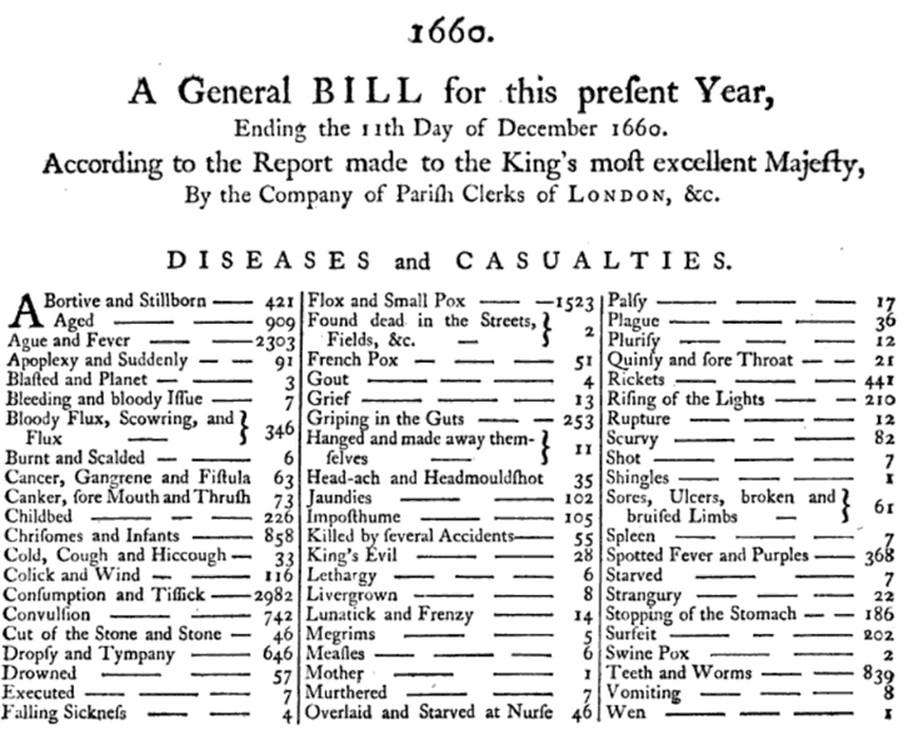
\includegraphics[width=1\linewidth]{images/StandardizedVocabularies/bill} 

}

\caption{1660年のロンドン死亡報告書には、その時代に知られていた62の疾患の分類システムを使用して住民の死因が示されています。}\label{fig:bill}
\end{figure}

それ以来、分類の規模と複雑性は大幅に拡大し、医療の他の側面、例えば処置やサービス、薬剤、医療デバイスなどにも広がりました。主な原則は変わっていません:つまり、患者データを収集、分類、分析するためにいくつかの医療コミュニティが合意した管理されたボキャブラリ、専門用語、階層やオントロジーです。これらの多くのボキャブラリは、公的あるいは政府機関によって長期的に管理されます。例えば、世界保健機関(WHO)は最近第11版(ICD11)が追加された「国際疾病分類(ICD)」を作成しています。各国の政府は、ICD10CM(米国)、ICD10GM(ドイツ)など、各国独自のバージョンを作成しています。政府はまた、薬品のマーケティングと販売を管理し、認証された薬剤の国家リポジトリを維持しています。ボキャブラリは民間部門でも、商業製品として、あるいはEHRシステムや保険請求報告書作成などの社内利用のために使用されています。

その結果、各国、各地域、医療制度、医療機関は、それぞれ独自の分類法を持つ傾向にあり、それは使用される場所でのみ関連性がある可能性が高いものです。こうした無数のボキャブラリが、使用されるシステムの相互運用性を妨げています。標準化は、患者データの交換を可能にし、世界レベルでの医療データ分析を可能にし、パフォーマンス特性や品質評価を含む体系化された標準化された研究を可能にする鍵となります。この問題に対処するため、多国籍の組織が設立され、前述のWHOや、標準病名(SNOMED)や、論理観察識別子名とコード(LOINC)などの幅広い標準の作成を開始しました。米国では、Health IT Standards Committee (HITAC) が、SNOMED、LOINC、および薬剤用ボキャブラリであるRxNormを、さまざまな組織間で全国規模の医療情報交換を行う共通プラットフォームで使用するための標準として、National Coordinator for Health IT (ONC) に推奨しています。

OHDSIは、観察研究のためのグローバルスタンダードであるOMOP CDMを開発しました。OMOP標準化ボキャブラリは、CDMの一部として、主に次の2つの目的で利用できます。

\begin{itemize}
\item
  コミュニティで使用されるすべてのボキャブラリの共通リポジトリ
\item
  研究使用のための標準化とマッピング
\end{itemize}

標準化ボキャブラリはコミュニティに無料で提供されており、OMOP CDMインスタンスでは\textbf{必須の参照テーブルとして使用する必要}があります。

\subsection{標準化ボキャブラリの構築}\label{ux6a19ux6e96ux5316ux30dcux30adux30e3ux30d6ux30e9ux30eaux306eux69cbux7bc9}

標準化ボキャブラリのすべてのボキャブラリは、共通の形式に統合されています。これにより、研究者が元のボキャブラリの複数の異なる形式とライフサイクルの慣例を理解して扱う必要がなくなります。すべてのボキャブラリは定期的に更新され、Pallasシステムを使用して統合されます\footnote{\url{https://github.com/OHDSI/Vocabulary-v5.0}}。これは、全体のOMOP CDMワークグループの一部であるOHDSIボキャブラリチームによって構築と運営がなされています。誤りを見つけた場合は、OHDSIフォーラム\footnote{\url{https://forums.ohdsi.org}}またはCDM GitHubページ\footnote{\url{https://github.com/OHDSI/CommonDataModel/issues}}に投稿して、私たちのリソースを改善するのにご協力ください。 \index{Pallas system}

\subsection{標準化ボキャブラリへのアクセス}\label{accessVocabularies}

標準化ボキャブラリを得るために、自分でPallasを実行する必要はありません。代わりに、ATHENA\footnote{\url{http://athena.ohdsi.org}}から最新バージョンをダウンロードし、ローカルデータベースにロードできます。ATHENAでは、ボキャブラリのファセット検索も可能です。 \index{ATHENA} \index{standardized vocabularies!download} \index{standardized vocabularies!search}

OMOP CDMのボキャブラリをすべて選んで、標準化されたボキャブラリテーブルのすべてを含むzipファイルをダウンロードします。標準コンセプトを持つボキャブラリ(第 \ref{standardConcepts} 部参照)と非常に一般的な使用法は事前に選択されています。提供元データで使用されているボキャブラリを追加します。著作権のあるボキャブラリには選択ボタンがありません。「ライセンス必要」ボタンをクリックしてそのようなボキャブラリをリストに組み込みます。ボキャブラリチームが連絡し、ライセンスを提示するか、適切な人々と連絡を取り合うためのサポートを提供します。

\subsection{ボキャブラリの元: 採用するか構築するか}\label{ux30dcux30adux30e3ux30d6ux30e9ux30eaux306eux5143-ux63a1ux7528ux3059ux308bux304bux69cbux7bc9ux3059ux308bux304b}

OHDSIは一般に、既存のボキャブラリを採用することを優先します。なぜなら、1)多くのボキャブラリがコミュニティ内で観察データに使用されているため、2)ボキャブラリの構築とメンテナンスは複雑で、成熟するためには多くの利害関係者の長期にわたる協力が必要だからです。このため、特定の組織がボキャブラリを提供しており、ボキャブラリは生成、廃止、統合、分割のライフサイクルの対象となります(第 \ref{conceptLifeCycle} 部参照)。現在、OHDSIはタイプコンセプト(例:コンディションタイプコンセプト)などの内部管理ボキャブラリのみを作成しています。唯一の例外は、米国以外でのみ使用される医薬品を対象とするRxNorm Extensionボキャブラリです(第\ref{rxNormExtension} 部参照)。

\section{コンセプト}\label{ux30b3ux30f3ux30bbux30d7ux30c8}

OMOP CDMの臨床イベントはすべてコンセプトとして表現されます。これらはデータレコードの基本的な構成要素であり、ほとんどのテーブルは、いくつかの例外を除いて完全に正規化されています。コンセプトはCONCEPTテーブルに格納されます(図 \ref{fig:concept} を参照)。\index{concept}

\begin{figure}

{\centering 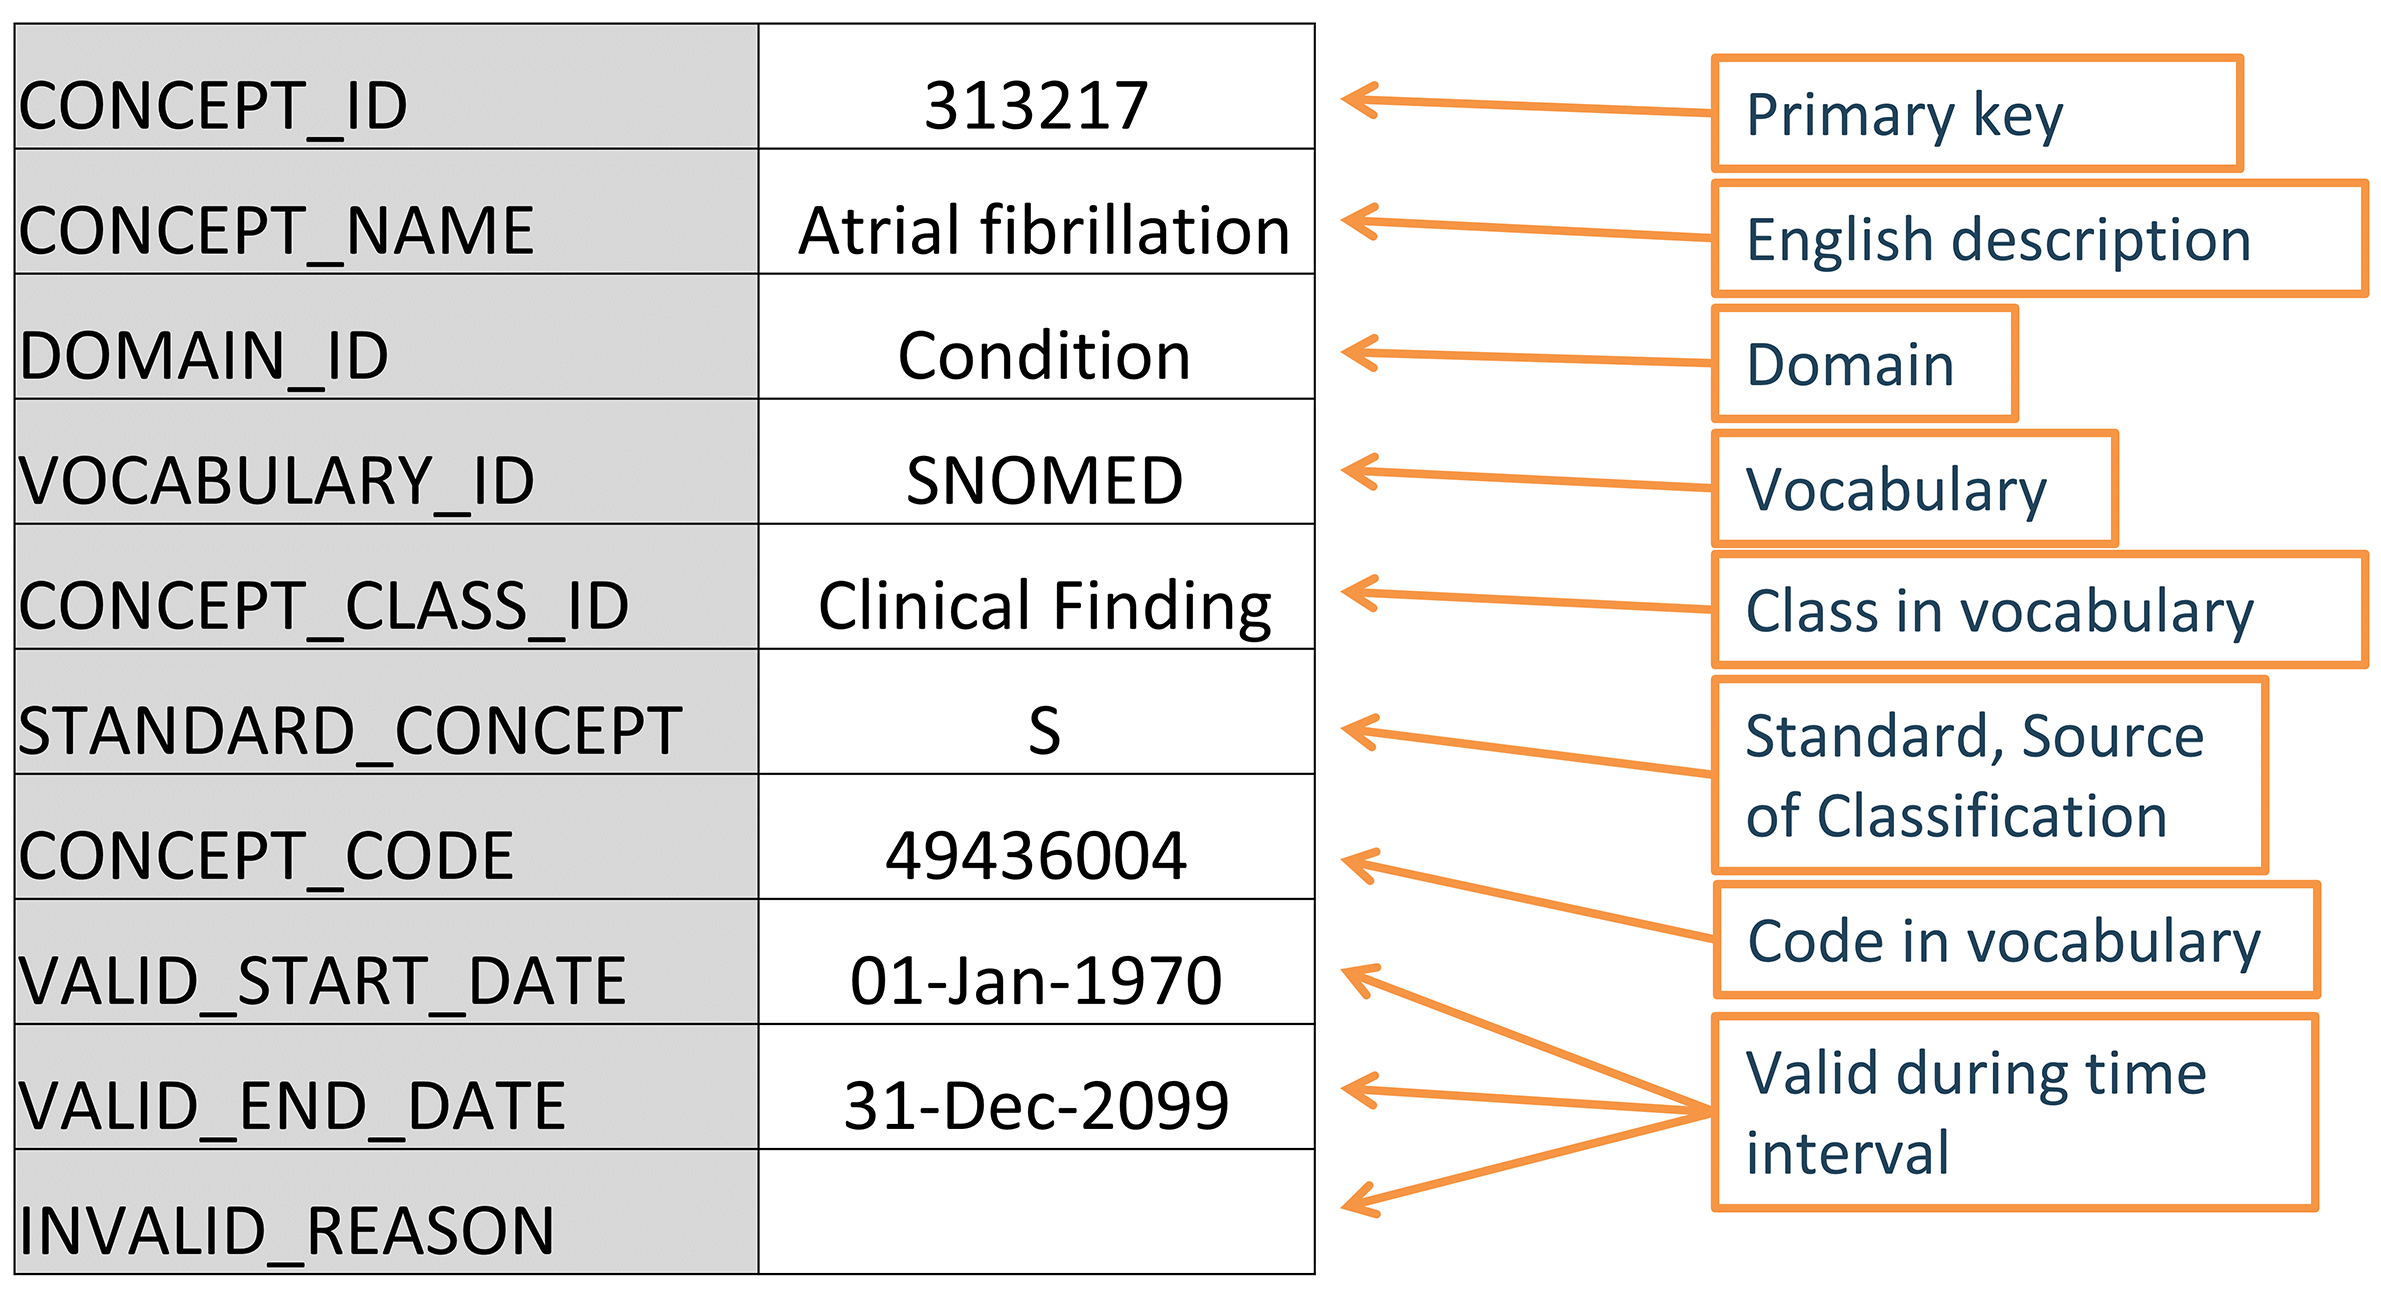
\includegraphics[width=0.9\linewidth]{images/StandardizedVocabularies/concept} 

}

\caption{OMOP CDMにおける標準化ボキャブラリコンセプトの標準的な表現。提示されている例は心房細動のSNOMEDコードに対するCONCEPTテーブルのレコードです。}\label{fig:concept}
\end{figure}

このシステムは\textbf{包括的}であることを意味し、患者の医療体験に関連するすべてのイベント(例:コンディション、処置、薬剤曝露など)や医療システムの一部の管理情報(例:ビジット、医療施設など)をカバーするのに十分なコンセプトが存在します。

\subsection{コンセプトID}\label{ux30b3ux30f3ux30bbux30d7ux30c8id}

各コンセプトにはプライマリキーとして使用されるコンセプトIDが割り当てられます。この無意味な整数IDは、CDMのイベントテーブルにデータを記録する際に使用され、元のボキャブラリコードではありません。 \index{concept!identifier}

\subsection{コンセプト名}\label{ux30b3ux30f3ux30bbux30d7ux30c8ux540d}

各コンセプトには1つの名称が割り当てられます。名称は常に英語表記です。名称はボキャブラリのソースからインポートされます。ソースのボキャブラリに複数の名称がある場合は、最も表現力のある名称が選択され、残りの名称は同じCONCEPT\_IDキーの下にあるCONCEPT\_SYNONYMテーブルに保存されます。英語以外の名称もCONCEPT\_SYNONYMに記録され、LANGUAGE\_CONCEPT\_IDフィールドに適切な言語のコンセプトIDが含まれます。名前の長さは255文字です。つまり、非常に長い名前は切り捨てられ、完全版は別の同義語として記録され、最大1000文字まで保持できます。

\subsection{ドメイン}\label{conceptDomains}

各コンセプトにはDOMAIN\_IDフィールドにドメインが割り当てられています。これは数値のCONCEPT\_IDとは対照的に、ドメイン用の小文字表記の大文字小文字区別を区別する一意の英数字IDです。例として、「Condition」、「Drug」、「Procedure」、「Visit」、「Device」、「Specimen」などのドメイン識別子があります。曖昧なコンセプトや事前にコード化された(組み合わせ)コンセプトは複合ドメインに属することがありますが、標準コンセプト(第\ref{standardConcepts}部参照)は常に単一のドメインが割り当てられます。ドメインは、臨床イベントやイベント属性がどのCDMテーブルやフィールドに記録されるかを指示します。 ドメインの割り当ては、\href{https://github.com/ohDSI/vocabulary-v5.0}{Pallas}に示されているヒューリスティックな手法を使用してボキャブラリの取り込み中に実行されるOMOP固有の機能です。ソースボキャブラリは、さまざまな程度で混合ドメインのコードを組み合わせる傾向があります(図 \ref{fig:domains} 参照)。\index{domain!concept}

\begin{figure}

{\centering 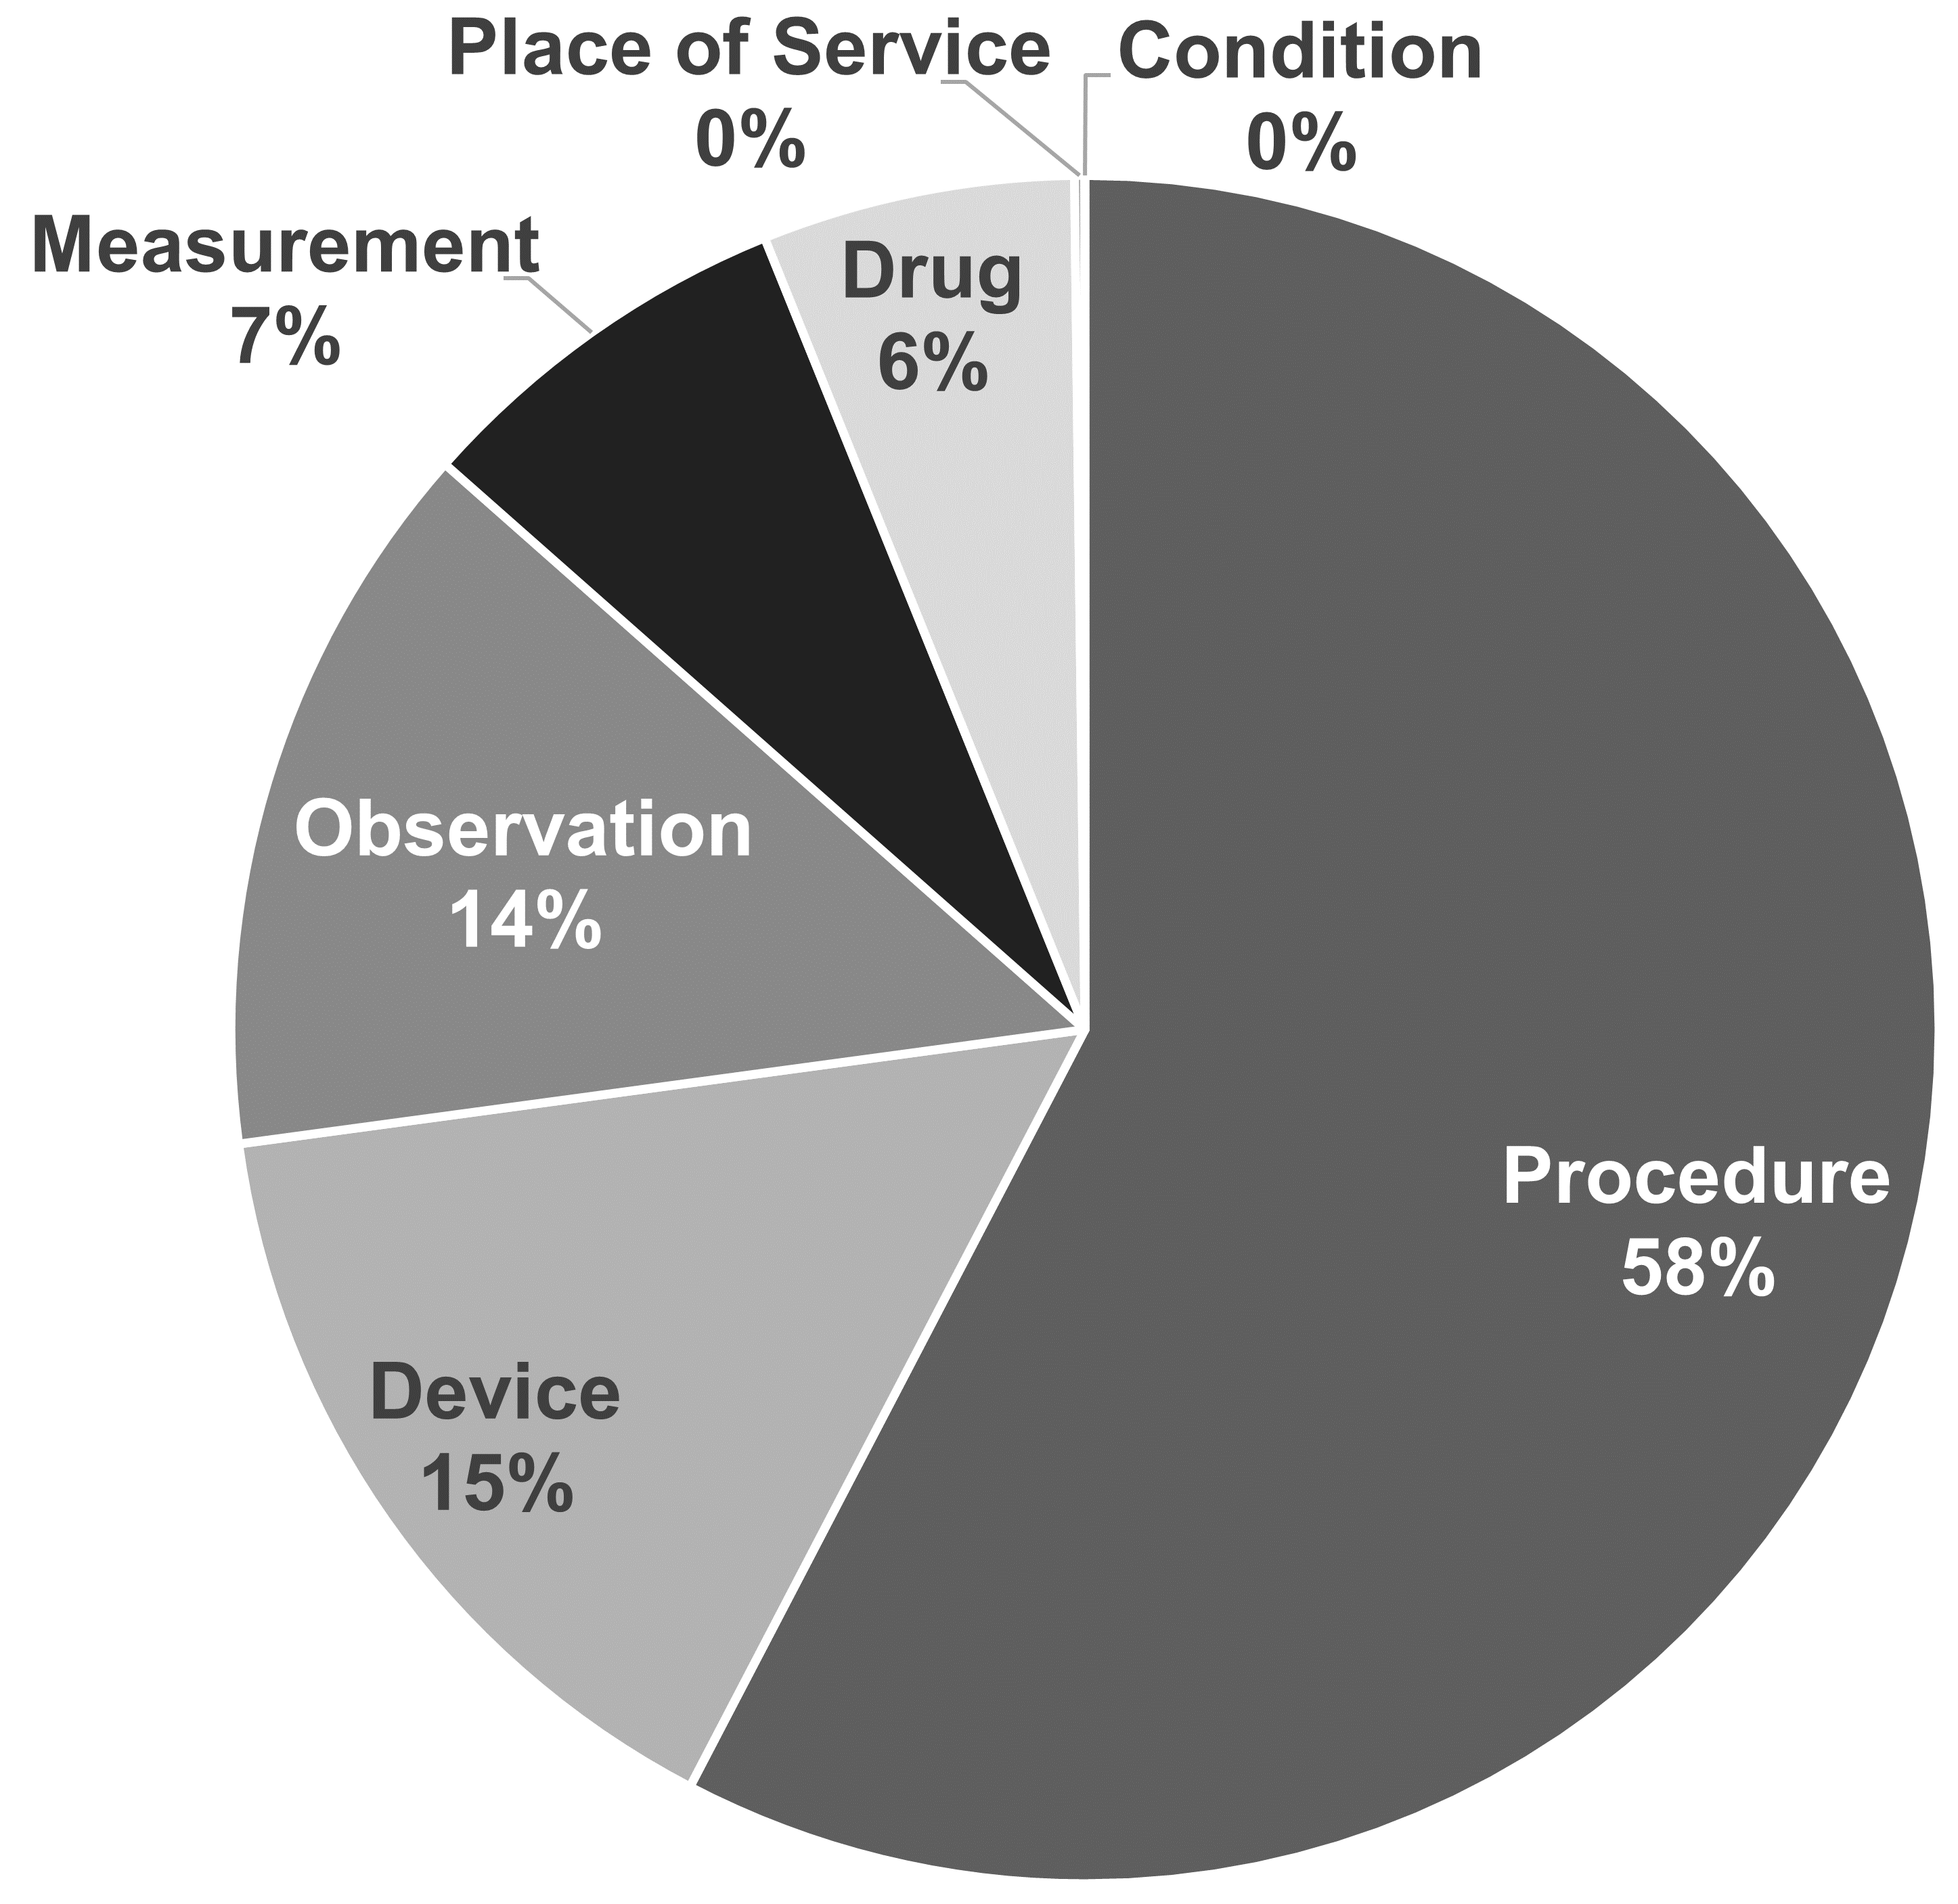
\includegraphics[width=0.7\linewidth]{images/StandardizedVocabularies/domains} 

}

\caption{処置ボキャブラリCPT4およびHCPCSにおけるドメインの割り当て。直感的には、これらのボキャブラリは単一のドメインのコードとコンセプトを含むべきですが、実際には混在しています。}\label{fig:domains}
\end{figure}

ドメインのヒューリスティックは、ドメインの定義に従います。これらの定義はCDMのテーブルとフィールド定義から派生しています(第 \ref{CommonDataModel}部参照)。ヒューリスティックは完全ではなく、グレーゾーンも存在します(第 \ref{specialSituations} 部「特別な状況」参照)。ドメインが誤って割り当てられているコンセプトがある場合、\href{https://forums.ohdsi.org}{フォーラム}または\href{https://github.com/OHDSI/CommonDataModel/issues}{CDM問題}の投稿を通じて報告し、プロセスの改善に貢献してください。

\subsection{ボキャブラリ}\label{ux30dcux30adux30e3ux30d6ux30e9ux30ea}

各ボキャブラリには短い大文字小文字区別のない一意の英数字IDが割り当てられており、通常はダッシュを省略したボキャブラリの略称に続きます。例えば、ICD-9-CMのボキャブラリIDは「ICD9CM」です。現在、OHDSIでサポートされているボキャブラリは111あり、そのうち78は外部ソースから採用されたもので、残りはOMOP内部のボキャブラリです。これらのボキャブラリは通常、四半期ごとに更新されます。ボキャブラリのソースおよびバージョンは、ボキャブラリリファレンスファイルで定義されています。 \index{vocabulary}

\subsection{コンセプトクラス}\label{ux30b3ux30f3ux30bbux30d7ux30c8ux30afux30e9ux30b9}

一部のボキャブラリでは、大文字と小文字を区別する固有の英数字IDによって表されるコードまたはコンセプトを分類しています。例えば、SNOMEDには33のこのようなコンセプトクラスがあり、SNOMEDではこれを「意味タグ」と呼んでいます。臨床所見、社会的背景、身体構造などです。これらはコンセプトの垂直的な区分です。MedDRAやRxNormなどの他のものには、階層化された階層構造の水平レベルを分類するコンセプトクラスがあります。HCPCSなどのコンセプトクラスを持たないボキャブラリでは、ボキャブラリIDをコンセプトクラスIDとして使用します。\index{concept!class}

\begin{longtable}[]{@{}
  >{\raggedright\arraybackslash}p{(\columnwidth - 2\tabcolsep) * \real{0.5000}}
  >{\raggedright\arraybackslash}p{(\columnwidth - 2\tabcolsep) * \real{0.5000}}@{}}
\caption{\label{tab:sublassification} コンセプトクラスにおける水平および垂直のサブ分類原則を持つボキャブラリと持たないボキャブラリ}\tabularnewline
\toprule\noalign{}
\begin{minipage}[b]{\linewidth}\raggedright
コンセプトクラスの区分原則
\end{minipage} & \begin{minipage}[b]{\linewidth}\raggedright
ボキャブラリ
\end{minipage} \\
\midrule\noalign{}
\endfirsthead
\toprule\noalign{}
\begin{minipage}[b]{\linewidth}\raggedright
コンセプトクラスの区分原則
\end{minipage} & \begin{minipage}[b]{\linewidth}\raggedright
ボキャブラリ
\end{minipage} \\
\midrule\noalign{}
\endhead
\bottomrule\noalign{}
\endlastfoot
水平 & すべての薬剤ボキャブラリ、ATC、CDT、Episode、HCPCS、HemOnc、ICDs、MedDRA、OSM、国勢調査 \\
垂直 & CIEL、HES専門、ICDO3、MeSH、NAACCR、NDFRT、OPCS4、PCORNET、Plan、PPI、Provider、SNOMED、SPL、UCUM \\
混在 & CPT4、ISBT、LOINC \\
なし & APC、すべてのタイプコンセプト、民族性、OXMIS、種族、収益コード、スポンサー、供給者、UB04、訪問 \\
\end{longtable}

水平コンセプトクラスにより、特定の階層レベルを決定することができます。たとえば、医薬品ボキャブラリのRxNormにおけるコンセプトクラス「Ingredient」は階層の最上位レベルを定義します。垂直モデルでは、コンセプトクラスのメンバーは最上位から最下位までの任意の階層レベルにすることができます。

\subsection{標準コンセプト}\label{standardConcepts}

各臨床イベントを表す1つのコンセプトが標準として指定されます。例えば、MESHコードD001281、CIELコード148203、SNOMEDコード49436004、ICD9CMコード427.31、ReadコードG573000はすべて、コンディションドメインで「心房細動」を定義していますが、SNOMEDの概念のみが標準であり、データ内のコンディションを表します。他のものは非標準またはソースコンセプトとして指定され、標準コンセプトにマッピングされています。標準コンセプトはSTANDARD\_CONCEPTフィールドに「S」で示されます。そして、CDMフィールドの末尾が「\_CONCEPT\_ID」となっているデータ記録には、これらの標準コンセプトのみが使用されます。 \index{standard concept}

\subsection{非標準コンセプト}\label{ux975eux6a19ux6e96ux30b3ux30f3ux30bbux30d7ux30c8}

非標準コンセプトは臨床イベントを表現するためには使用されませんが、標準化されたボキャブラリの一部であり、ソースデータに頻繁に見られます。そのため、それらは「ソースコンセプト」とも呼ばれます。ソースコンセプトを標準コンセプトに変換するプロセスは「マッピング」と呼ばれます(セクション \ref{conceptMapping}参照)。非標準コンセプトにはSTANDARD\_CONCEPTフィールドに値がありません(NULL)。

\subsection{分類コンセプト}\label{ux5206ux985eux30b3ux30f3ux30bbux30d7ux30c8}

これらのコンセプトは標準ではなく、したがってデータを表現するためには使用されませんが、標準コンセプトと階層的に関連しており、そのため階層クエリを実行するために使用できます。たとえば、MedDRAコード10037908のすべての子孫をクエリする場合(MedDRAライセンスを取得していないユーザーには表示されません。アクセス制限については第 \ref{accessVocabularies} 部参照)では、標準のSNOMEDコンセプト「心房細動」を取得します(CONCEPT\_ANCESTORテーブルを使用した階層クエリについては第 \ref{conceptAncestor}部を参照) - 図 \ref{fig:hierarchy} を参照。 \index{classification concept}

\begin{figure}

{\centering 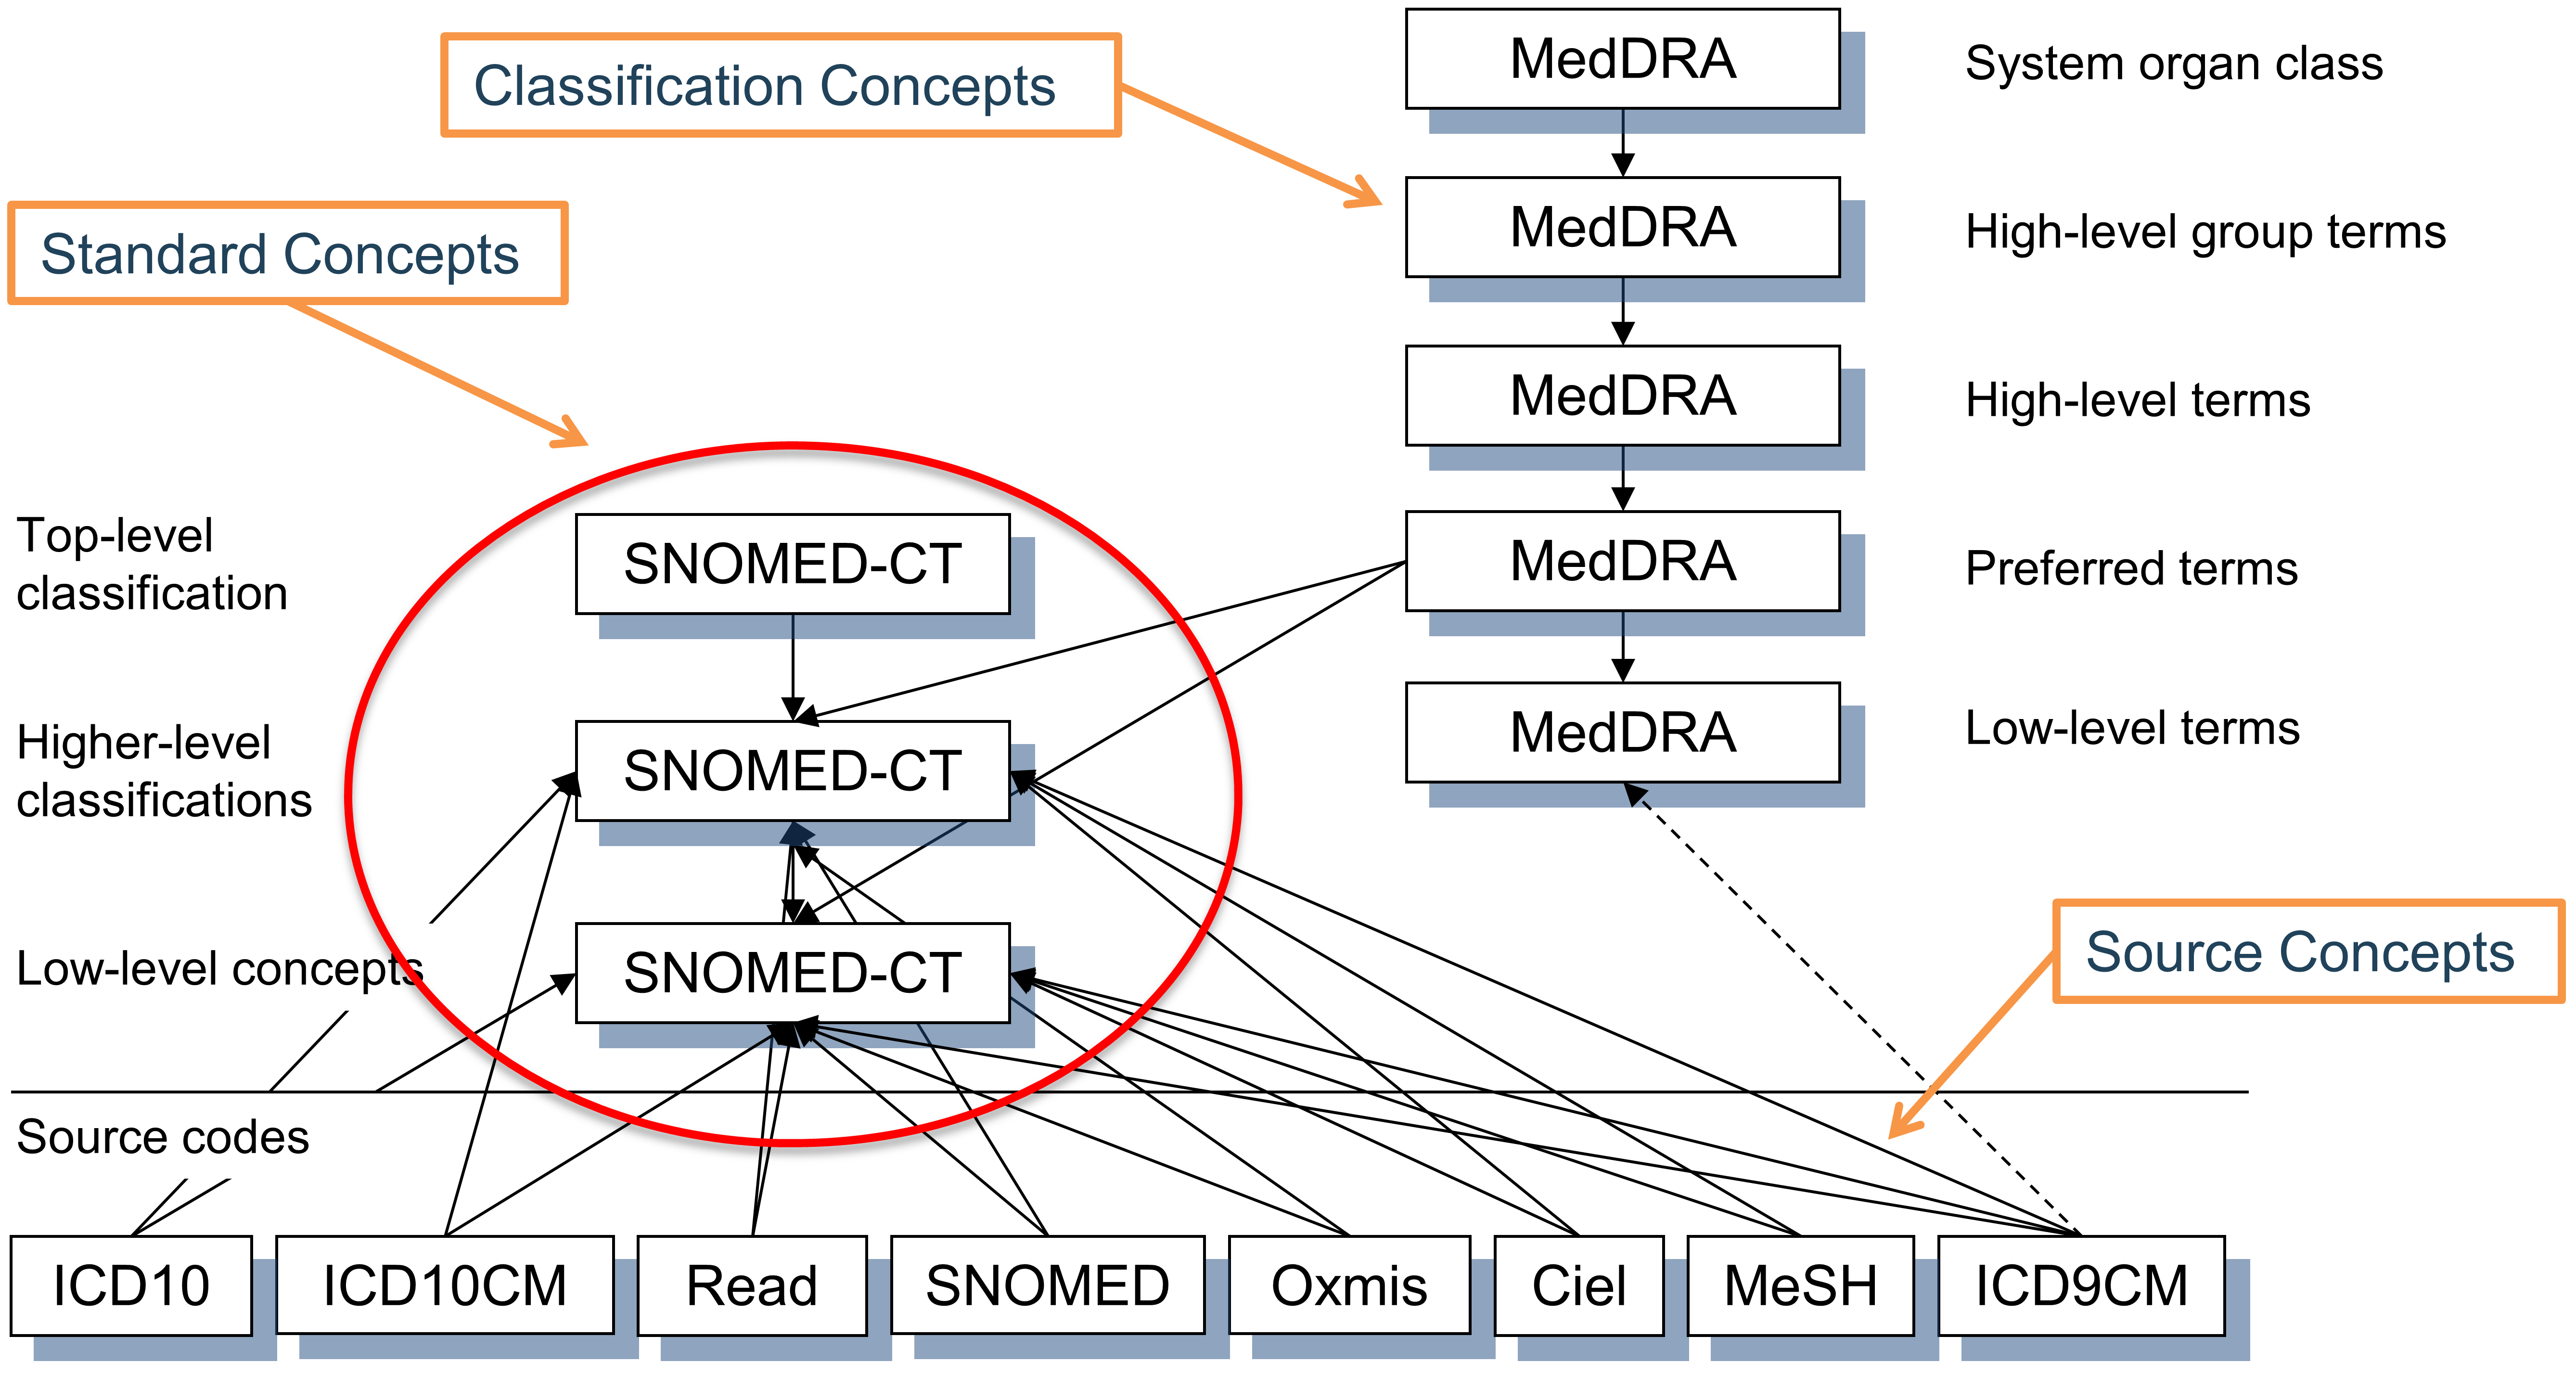
\includegraphics[width=1\linewidth]{images/StandardizedVocabularies/hierarchy} 

}

\caption{コンディションドメインにおける標準、非標準ソースおよび分類コンセプトとその階層関係。SNOMEDはほとんどの標準コンディションコンセプトに使用されており(いくつかの腫瘍関連コンセプトはICDO3から派生)、MedDRAコンセプトは階層分類コンセプトに使用されており、他のすべてのボキャブラリは非標準またはソースコンセプトを含み、階層には含まれません。}\label{fig:hierarchy}
\end{figure}

標準、非標準、分類のコンセプトの選択は、通常各ドメインごとにボキャブラリレベルで行われます。これはコンセプトの質、組込みの階層、ボキャブラリが宣言された目的に基づいています。また、すべてのボキャブラリのコンセプトが標準コンセプトとして使用されているわけではありません。各ドメインごとに別々に指定されており、各コンセプトはアクティブである必要があります(第 \ref{conceptLifeCycle} 部参照)し、異なるボキャブラリから同じ意味を持つ複数のコンセプトが競合する場合には、優先順位が設定される場合もあります。 つまり、「標準ボキャブラリ」というものは存在しません。 例については表 \ref{tab:vocabList} を参照ください。

\begin{longtable}[]{@{}
  >{\raggedright\arraybackslash}p{(\columnwidth - 6\tabcolsep) * \real{0.2500}}
  >{\raggedright\arraybackslash}p{(\columnwidth - 6\tabcolsep) * \real{0.2500}}
  >{\raggedright\arraybackslash}p{(\columnwidth - 6\tabcolsep) * \real{0.2500}}
  >{\raggedright\arraybackslash}p{(\columnwidth - 6\tabcolsep) * \real{0.2500}}@{}}
\caption{\label{tab:vocabList} 標準/非標準/分類コンセプトの割り当てに利用するボキャブラリのリスト}\tabularnewline
\toprule\noalign{}
\begin{minipage}[b]{\linewidth}\raggedright
ドメイン
\end{minipage} & \begin{minipage}[b]{\linewidth}\raggedright
標準コンセプトのためのボキャブラリ
\end{minipage} & \begin{minipage}[b]{\linewidth}\raggedright
ソースコンセプトのためのボキャブラリ
\end{minipage} & \begin{minipage}[b]{\linewidth}\raggedright
分類コンセプトのためのボキャブラリ
\end{minipage} \\
\midrule\noalign{}
\endfirsthead
\toprule\noalign{}
\begin{minipage}[b]{\linewidth}\raggedright
ドメイン
\end{minipage} & \begin{minipage}[b]{\linewidth}\raggedright
標準コンセプトのためのボキャブラリ
\end{minipage} & \begin{minipage}[b]{\linewidth}\raggedright
ソースコンセプトのためのボキャブラリ
\end{minipage} & \begin{minipage}[b]{\linewidth}\raggedright
分類コンセプトのためのボキャブラリ
\end{minipage} \\
\midrule\noalign{}
\endhead
\bottomrule\noalign{}
\endlastfoot
コンディション & SNOMED, ICDO3 & SNOMED Veterinary & MedDRA \\
処置 & SNOMED, CPT4, HCPCS, ICD10PCS, ICD9Proc, OPCS4 & SNOMED Veterinary, HemOnc, NAACCR & 現時点ではなし \\
測定 & SNOMED, LOINC & SNOMED Veterinary, NAACCR, CPT4, HCPCS, OPCS4, PPI & 現時点ではなし \\
薬剤 & RxNorm, RxNorm Extension, CVX & HCPCS, CPT4, HemOnc, NAACCR & ATC \\
デバイス & SNOMED & 他のボキャブラリ、現在は標準化されていない & 現時点ではなし \\
観察 & SNOMED & 他のボキャブラリ & 現時点ではなし \\
ビジット & CMS Place of Service, ABMT, NUCC & SNOMED, HCPCS, CPT4, UB04 & 現時点ではなし \\
\end{longtable}

\subsection{コンセプトコード}\label{ux30b3ux30f3ux30bbux30d7ux30c8ux30b3ux30fcux30c9}

コンセプトコードはソースボキャブラリで使用される識別子です。たとえば、ICD9CMまたはNDCコードはこのフィールドに保存され、OMOPテーブルはCONCEPTテーブルへの外部キーとしてコンセプトIDを使用します。その理由は、ボキャブラリを超えて名前空間が重複するためです。つまり、同じコードが異なるボキャブラリに存在し、それぞれ全く異なる意味を持つ可能性があるためです(表 \ref{tab:code1001} 参照)。\index{concept!code}

\begin{longtable}[]{@{}
  >{\raggedright\arraybackslash}p{(\columnwidth - 10\tabcolsep) * \real{0.1667}}
  >{\raggedright\arraybackslash}p{(\columnwidth - 10\tabcolsep) * \real{0.1667}}
  >{\raggedright\arraybackslash}p{(\columnwidth - 10\tabcolsep) * \real{0.1667}}
  >{\raggedright\arraybackslash}p{(\columnwidth - 10\tabcolsep) * \real{0.1667}}
  >{\raggedright\arraybackslash}p{(\columnwidth - 10\tabcolsep) * \real{0.1667}}
  >{\raggedright\arraybackslash}p{(\columnwidth - 10\tabcolsep) * \real{0.1667}}@{}}
\caption{\label{tab:code1001} 同じコンセプトコード1001を持つが、異なるボキャブラリ、ドメイン、コンセプトクラスのコンセプト}\tabularnewline
\toprule\noalign{}
\begin{minipage}[b]{\linewidth}\raggedright
コンセプトID
\end{minipage} & \begin{minipage}[b]{\linewidth}\raggedright
コンセプトコード
\end{minipage} & \begin{minipage}[b]{\linewidth}\raggedright
コンセプト名
\end{minipage} & \begin{minipage}[b]{\linewidth}\raggedright
ドメインID
\end{minipage} & \begin{minipage}[b]{\linewidth}\raggedright
ボキャブラリID
\end{minipage} & \begin{minipage}[b]{\linewidth}\raggedright
コンセプトクラス
\end{minipage} \\
\midrule\noalign{}
\endfirsthead
\toprule\noalign{}
\begin{minipage}[b]{\linewidth}\raggedright
コンセプトID
\end{minipage} & \begin{minipage}[b]{\linewidth}\raggedright
コンセプトコード
\end{minipage} & \begin{minipage}[b]{\linewidth}\raggedright
コンセプト名
\end{minipage} & \begin{minipage}[b]{\linewidth}\raggedright
ドメインID
\end{minipage} & \begin{minipage}[b]{\linewidth}\raggedright
ボキャブラリID
\end{minipage} & \begin{minipage}[b]{\linewidth}\raggedright
コンセプトクラス
\end{minipage} \\
\midrule\noalign{}
\endhead
\bottomrule\noalign{}
\endlastfoot
35803438 & 1001 & 顆粒球コロニー刺激因子 & 薬剤 & HemOnc & コンポーネントクラス \\
35942070 & 1001 & AJCC TNM Clin T & 測定 & NAACCR & NAACCR変数 \\
1036059 & 1001 & アンチピリン & 薬剤 & RxNorm & 成分 \\
38003544 & 1001 & レジデンシャル治療 - 精神科 & 収益コード & 収益コード & 収益コード \\
43228317 & 1001 & アセプロメタジンマレイン酸塩 & 薬剤 & BDPM & 成分 \\
45417187 & 1001 & ブロムフェニラミンマレイン酸塩、10 mg/ml注射用溶液 & 薬剤 & Multum & Multum \\
45912144 & 1001 & 血清 & 標本 & CIEL & 標本 \\
\end{longtable}

\subsection{ライフサイクル}\label{conceptLifeCycle}

ボキャブラリは、固定されたコードセットを持つ恒久的なコーパスであることはまれです。その代わり、コードやコンセプトは追加され、廃止されていきます。OMOP CDMは、患者の経時的データをサポートするモデルであり、過去に使用されていたが現在は使用されていないコンセプトをサポートする必要があるだけでなく、新しいコンセプトをサポートし、そのコンセプトを文脈に配置する必要があります。CONCEPTテーブルには、ライフサイクルのステータスを記述する3つのフィールドがあります。VALID\_START\_DATE、VALID\_END\_DATE、INVALID\_REASONです。これらの値は、コンセプトのライフサイクルのステータスによって異なります。:

\begin{itemize}
\tightlist
\item
  \textbf{アクティブまたは新しいコンセプト}

  \begin{itemize}
  \tightlist
  \item
    説明: 使用中のコンセプト。
  \item
    VALID\_START\_DATE: コンセプトの生成日。不明の場合はボキャブラリへの取り込み日。不明の場合は1970-1-1。
  \item
    VALID\_END\_DATE: 「将来、定義されていない時点で無効になる可能性があるが、現在はアクティブである」ことを示す慣例として、2099年12月31日に設定。
  \item
    INVALID\_REASON: NULL
  \end{itemize}
\item
  \textbf{非推奨のコンセプトで後継なし}

  \begin{itemize}
  \tightlist
  \item
    説明: 非アクティブであり、標準として使用することはできない(第\ref{standardConcepts}部参照)。
  \item
    VALID\_START\_DATE: コンセプトの生成日。不明の場合はボキャブラリへの取り込み日。不明の場合は1970-1-1。
  \item
    VALID\_END\_DATE: 過去の廃止日。不明の場合はボキャブラリ内のコンセプトが欠落あるいは非アクティブに設定されたボキャブラリ更新日。
  \item
    INVALID\_REASON: ``D''
  \end{itemize}
\item
  \textbf{後継コンセプトとともにアップグレードされたコンセプト}

  \begin{itemize}
  \tightlist
  \item
    説明: コンセプトは非アクティブだが、後継コンセプトが定義されています。通常は、重複排除が行われたコンセプトです。
  \item
    VALID\_START\_DATE: コンセプトの生成日。不明の場合はボキャブラリへの取り込み日、もしくは1970-1-1。
  \item
    VALID\_END\_DATE: アップグレードが行われた過去の年月日。不明の場合は、アップグレードが含まれたボキャブラリのリフレッシュ日。
  \item
    INVALID\_REASON: ``U''
  \end{itemize}
\item
  \textbf{別の新しいコンセプトで再利用されたコード}

  \begin{itemize}
  \tightlist
  \item
    説明: 非推奨のコンセプトコードが、新しいコンセプトで再利用されました。
  \item
    VALID\_START\_DATE: コンセプトの生成日。不明の場合はボキャブラリへの取り込み日、もしくは1970年1月1日。
  \item
    VALID\_END\_DATE: 非推奨であることを示す過去の日、またはそれがわからない場合は、ボキャブラリのコンセプトがなくなった、または非アクティブに設定されたボキャブラリ更新の日。
  \item
    INVALID\_REASON: ``R''
  \end{itemize}
\end{itemize}

一般に、コンセプトコードは再利用されません。しかし、特にHCPCS、NDC、DRGなど、このルールから外れるボキャブラリがいくつかあります。これらのボキャブラリでは、同じコンセプトコードが同じボキャブラリの複数のコンセプトに現れます。CONCEPT\_ID の値は一意です。これらの再使用されるコンセプトコードは、INVALID\_REASONフィールドに「R」が付され、VALID\_START\_DATEからVALID\_END\_DATEの期間は、同じコンセプトコードを持つコンセプトを区別するために使用されるべきです。

\section{関係}\label{ux95a2ux4fc2}

任意の2つのコンセプトは、そのドメインやボキャブラリーが同じであるかどうかに関係なく、定義された関係を持つことができます。関係の性質は、CONCEPT\_RELATIONSHIPテーブルのRELATIONSHIP\_IDフィールドにある、大文字小文字を区別する一意の英数字IDで示されます。関係は対称的であり、各関係には同等の関係が存在し、フィールドCONCEPT\_ID\_1とCONCEPT\_ID\_2の内容が入れ替わり、RELATIONSHIP\_IDはその逆に変更されます。たとえば、「Maps to」関係には反対の関係「Mapped from」があります。\index{concept!relationship}

CONCEPT\_RELATIONSHIPテーブルのレコードには、ライフサイクルフィールドRELATIONSHIP\_START\_DATE、RELATIONSHIP\_END\_DATE、INVALID\_REASONも含まれています。ただし、ATHENAを通じて利用可能なのはINVALID\_REASONがNULLのアクティブなレコードのみです。非アクティブな関係は内部処理のためにPallasシステムに保存されます。RELATIONSHIPテーブルは、全ての関係IDおよびその逆関係のリストを参照するためのものです。

\subsection{マッピング関係}\label{conceptMapping}

これらの関係は、非標準のコンセプトから標準コンセプトへの変換を提供し、2つの関係IDペアによってサポートされています(表 \ref{tab:mappingRelationships} を参照)。\index{concept!mapping}

\begin{longtable}[]{@{}
  >{\raggedright\arraybackslash}p{(\columnwidth - 2\tabcolsep) * \real{0.5000}}
  >{\raggedright\arraybackslash}p{(\columnwidth - 2\tabcolsep) * \real{0.5000}}@{}}
\caption{\label{tab:mappingRelationships} マッピング関係の種類}\tabularnewline
\toprule\noalign{}
\begin{minipage}[b]{\linewidth}\raggedright
関係IDペア
\end{minipage} & \begin{minipage}[b]{\linewidth}\raggedright
目的
\end{minipage} \\
\midrule\noalign{}
\endfirsthead
\toprule\noalign{}
\begin{minipage}[b]{\linewidth}\raggedright
関係IDペア
\end{minipage} & \begin{minipage}[b]{\linewidth}\raggedright
目的
\end{minipage} \\
\midrule\noalign{}
\endhead
\bottomrule\noalign{}
\endlastfoot
``Maps to''と''Mapped from'' & 標準コンセプトはそれ自身にマッピングされ、非標準コンセプトは標準コンセプトにマッピングされます。ほとんどの非標準コンセプトとすべての標準コンセプトは、標準コンセプトとの間にこの関係があります。前者は*\_SOURCE\_CONCEPT\_IDフィールド\emph{に、後者は}\_CONCEPT\_IDフィールド*に格納されます。分類コンセプトはマッピングされません。 \\
``Maps to value''と''Value mapped from'' & MEASUREMENTとOBSERVATIONテーブルのVALUE\_AS\_CONCEPT\_IDフィールドに配置する値を表すコンセプトへのマッピング。 \\
\end{longtable}

これらのマッピング関係の目的は、同等のコンセプト間の相互参照を可能にし、臨床イベントがOMOP CDMでどのように表現されるかを統一することです。これは標準化ボキャブラリの主要な成果です。

「同等のコンセプト」とは、同じ意味を持ち、さらに重要なことには、階層下位のコンセプトが同じ意味領域をカバーすることを意味します。同等のコンセプトが利用できず、コンセプトが標準でない場合、それはより広いコンセプトにマッピング(いわゆる「上方向マッピング」)されます。たとえば、ICD10CM W61.51「ガチョウに噛まれる」は、標準のコンディションコンセプトとして使用されるSNOMEDボキャブラリには同等のものがありません。代わりに、それはSNOMED 217716004「鳥に突かれる」にマッピングされ、コンテキストとしての鳥がガチョウであるという情報が失われます。上方向マッピングは、情報の損失が標準的な研究用途には無関係であるとみなされる場合にのみ使用されます。

一部のマッピングでは、ソースコンセプトが複数の標準コンセプトにリンクされます。たとえば、ICD9CM 070.43「肝性昏睡を伴うE型肝炎」は、SNOMED 235867002「急性E型肝炎」とSNOMED 72836002「肝性昏睡」の両方にマッピングされます。これは、元のソースコンセプトが肝炎と昏睡という2つの状態のあらかじめ組み合わせられたものであるためです。SNOMEDにはその組み合わせがなく、その結果、ICD9CMレコードではマッピングされた標準コンセプトそれぞれに対して2つのレコードが作成されます。

「Maps to value」関係は、エンティティ-属性-値(EAV)モデルに従ってOMOP CDMテーブルの値を分割することを目的としています。これは次の状況で発生します:

\begin{itemize}
\tightlist
\item
  検査値と結果値からなる測定値
\item
  本人または家族の病歴
\item
  物質に対するアレルギー
\item
  予防接種の必要性
\end{itemize}

このような状況では、ソースコンセプトは属性(テストまたは履歴)と値(テスト結果または疾患)の組み合わせです。「Maps to」関係はこのソースを属性コンセプトにマッピングし、「Maps to value」は値コンセプトにマッピングします。例については図 \ref{fig:conceptValue}を参照ください。

\begin{figure}

{\centering 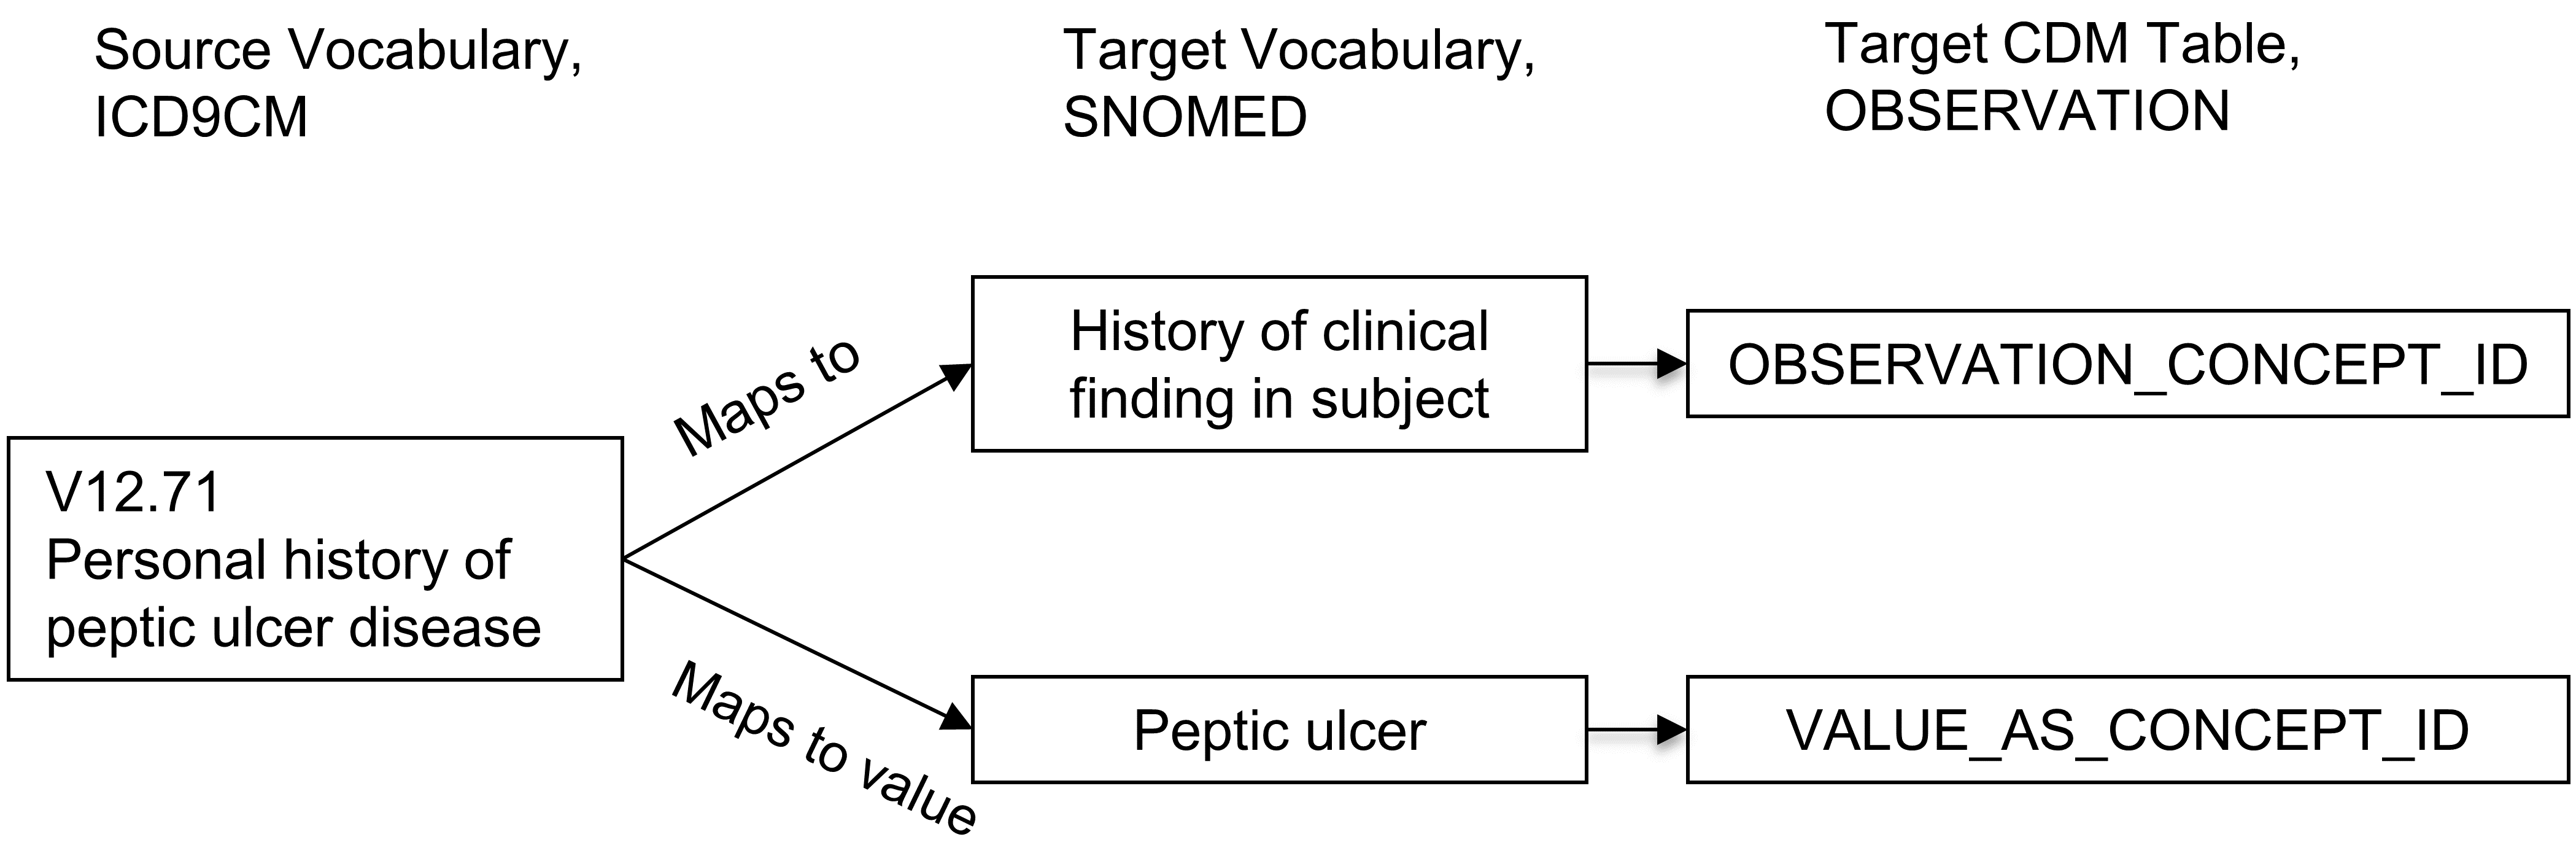
\includegraphics[width=1\linewidth]{images/StandardizedVocabularies/conceptValue} 

}

\caption{ソースコンセプトと標準コンセプト間の一対多のマッピング。事前に組み合わせられたコンセプトは2つのコンセプトに分割され、一つは属性(ここでは臨床所見の履歴)で、もう一つは値(消化性潰瘍)です。「Maps to」関係は測定または観察のドメインのコンセプトにマッピングされますが、「Maps to value」コンセプトにはドメインの制限はありません。}\label{fig:conceptValue}
\end{figure}

コンセプトのマッピングは、無料で提供され、ネットワーク研究を行うコミュニティの取り組みを支援するOMOP標準化ボキャブラリのもう一つの中心的な機能です。マッピング関係は外部ソースから導出されるか、ボキャブラリチームによって手動で維持されます。つまり、それらは完璧ではないということです。誤ったマッピング関係や好ましくないマッピング関係を見つけた場合は、\href{https://forums.ohdsi.org}{フォーラム}や\href{https://github.com/OHDSI/CommonDataModel/issues}{CDMの問題}の投稿を通じて報告し、プロセスの改善に協力することが重要です。

マッピング規則の詳細な説明は、OHDSI Wikiで見つけることができます\footnote{\url{https://www.ohdsi.org/web/wiki/doku.php?id=documentation:vocabulary:mapping}}。

\subsection{階層関係}\label{ux968eux5c64ux95a2ux4fc2}

階層関係は、「Is a」-「Subsumes」関係によって定義されます。階層関係は、子コンセプトが親コンセプトのすべての属性に加えて、1つ以上の追加属性またはより厳密に定義された属性を持つように定義されます。たとえば、SNOMED 49436004「心房細動」は、SNOMED 17366009「心房性不整脈」と「Is a」関係で関連しています。両コンセプトは、不整脈の種類(一方では細動と定義されているが、他方では定義されていない)を除いて、同一の属性セットを持っています。コンセプトは複数の親または複数の子コンセプトを持つことができます。この例では、SNOMED 49436004「心房細動」はSNOMED 40593004「細動」に対しても「Is a」に該当します。\index{concept!hierarchy}

\subsection{異なるボキャブラリーのコンセプト間の関係}\label{ux7570ux306aux308bux30dcux30adux30e3ux30d6ux30e9ux30eaux30fcux306eux30b3ux30f3ux30bbux30d7ux30c8ux9593ux306eux95a2ux4fc2}

これらの関係は通常、「ボキャブラリ A - ボキャブラリ B は同等」というタイプであり、ボキャブラリのオリジナルソースから提供されるか、OHDSIボキャブラリチームによって作成されます。それらは近似的なマッピングとして機能することが多いですが、より厳密に管理されたマッピング関係よりも制度が低い場合があります。高品質の同等関係(例えば、「ソース - RxNorm と同等」)は常に「Maps to」関係によって複製されます。

\subsection{同一ボキャブラリーのコンセプト間の関係}\label{ux540cux4e00ux30dcux30adux30e3ux30d6ux30e9ux30eaux30fcux306eux30b3ux30f3ux30bbux30d7ux30c8ux9593ux306eux95a2ux4fc2}

内部ボキャブラリ間の関係は通常、ボキャブラリ医療提供者によって提供されます。OHDSI Wikiの個々のボキャブラリの個々のボキャブラリー文書に完全な説明が記載されています\footnote{\url{https://www.ohdsi.org/web/wiki/doku.php?id=documentation:vocabulary}}。

これらの多くは、臨床イベント間の関係を定義しており、情報検索に使用することができます。例えば、尿道の障害は、「Finding site of(部位の検索)」関係に従うことで検索することができます(表 \ref{tab:findingSite} を参照)。

\begin{longtable}[]{@{}ll@{}}
\caption{\label{tab:findingSite} 尿道の「Finding site of」関係で、すべてこの解剖学的構造に位置する状態を示しています。}\tabularnewline
\toprule\noalign{}
CONCEPT\_ID\_1 & CONCEPT\_ID\_2 \\
\midrule\noalign{}
\endfirsthead
\toprule\noalign{}
CONCEPT\_ID\_1 & CONCEPT\_ID\_2 \\
\midrule\noalign{}
\endhead
\bottomrule\noalign{}
\endlastfoot
4000504 ``Urethra part'' & 36713433 ``部分的尿道重複'' \\
4000504 ``Urethra part'' & 433583 ``下部尿道裂孔'' \\
4000504 ``Urethra part'' & 443533 ``男性下部尿道裂孔'' \\
4000504 ``Urethra part'' & 4005956 ``女性下部尿道裂孔'' \\
\end{longtable}

これらの関係の質と網羅性は、元のボキャブラリーの質によって異なります。一般に、SNOMEDのような標準コンセプトを抽出するために使用されるボキャブラリは、より優れた管理がされているという理由で選択されるため、内部関係もより質の高いものとなる傾向があります。

\section{階層}\label{conceptAncestor}

ドメイン内では、標準および分類コンセプトは階層構造に整理され、CONCEPT\_ANCESTORテーブルに格納されます。これにより、コンセプトとその下位層に含まれるコンセプト(子孫)をすべてクエリして取得することが可能です。これらの子孫は祖先と同じ属性を持ちますが、追加の属性や、より詳細に定義された属性も持ちます。

CONCEPT\_ANCESTORテーブルは、階層関係を通じてつながっているすべてのコンセプトを網羅するCONCEPT\_RELATIONSHIPテーブルから自動的に構築されます。これらは ``Is a'' - ``Subsumes'' のペア(図 \ref{fig:conceptAncestor} 参照)であり、ボキャブラリ間の階層を結びつけるその他の関係です。関係が階層構築に参加するかは、関係IDごとにRELATIONSHIP参照テーブルのDEFINES\_ANCESTRYフラグによって定義されます。



\begin{figure}

{\centering 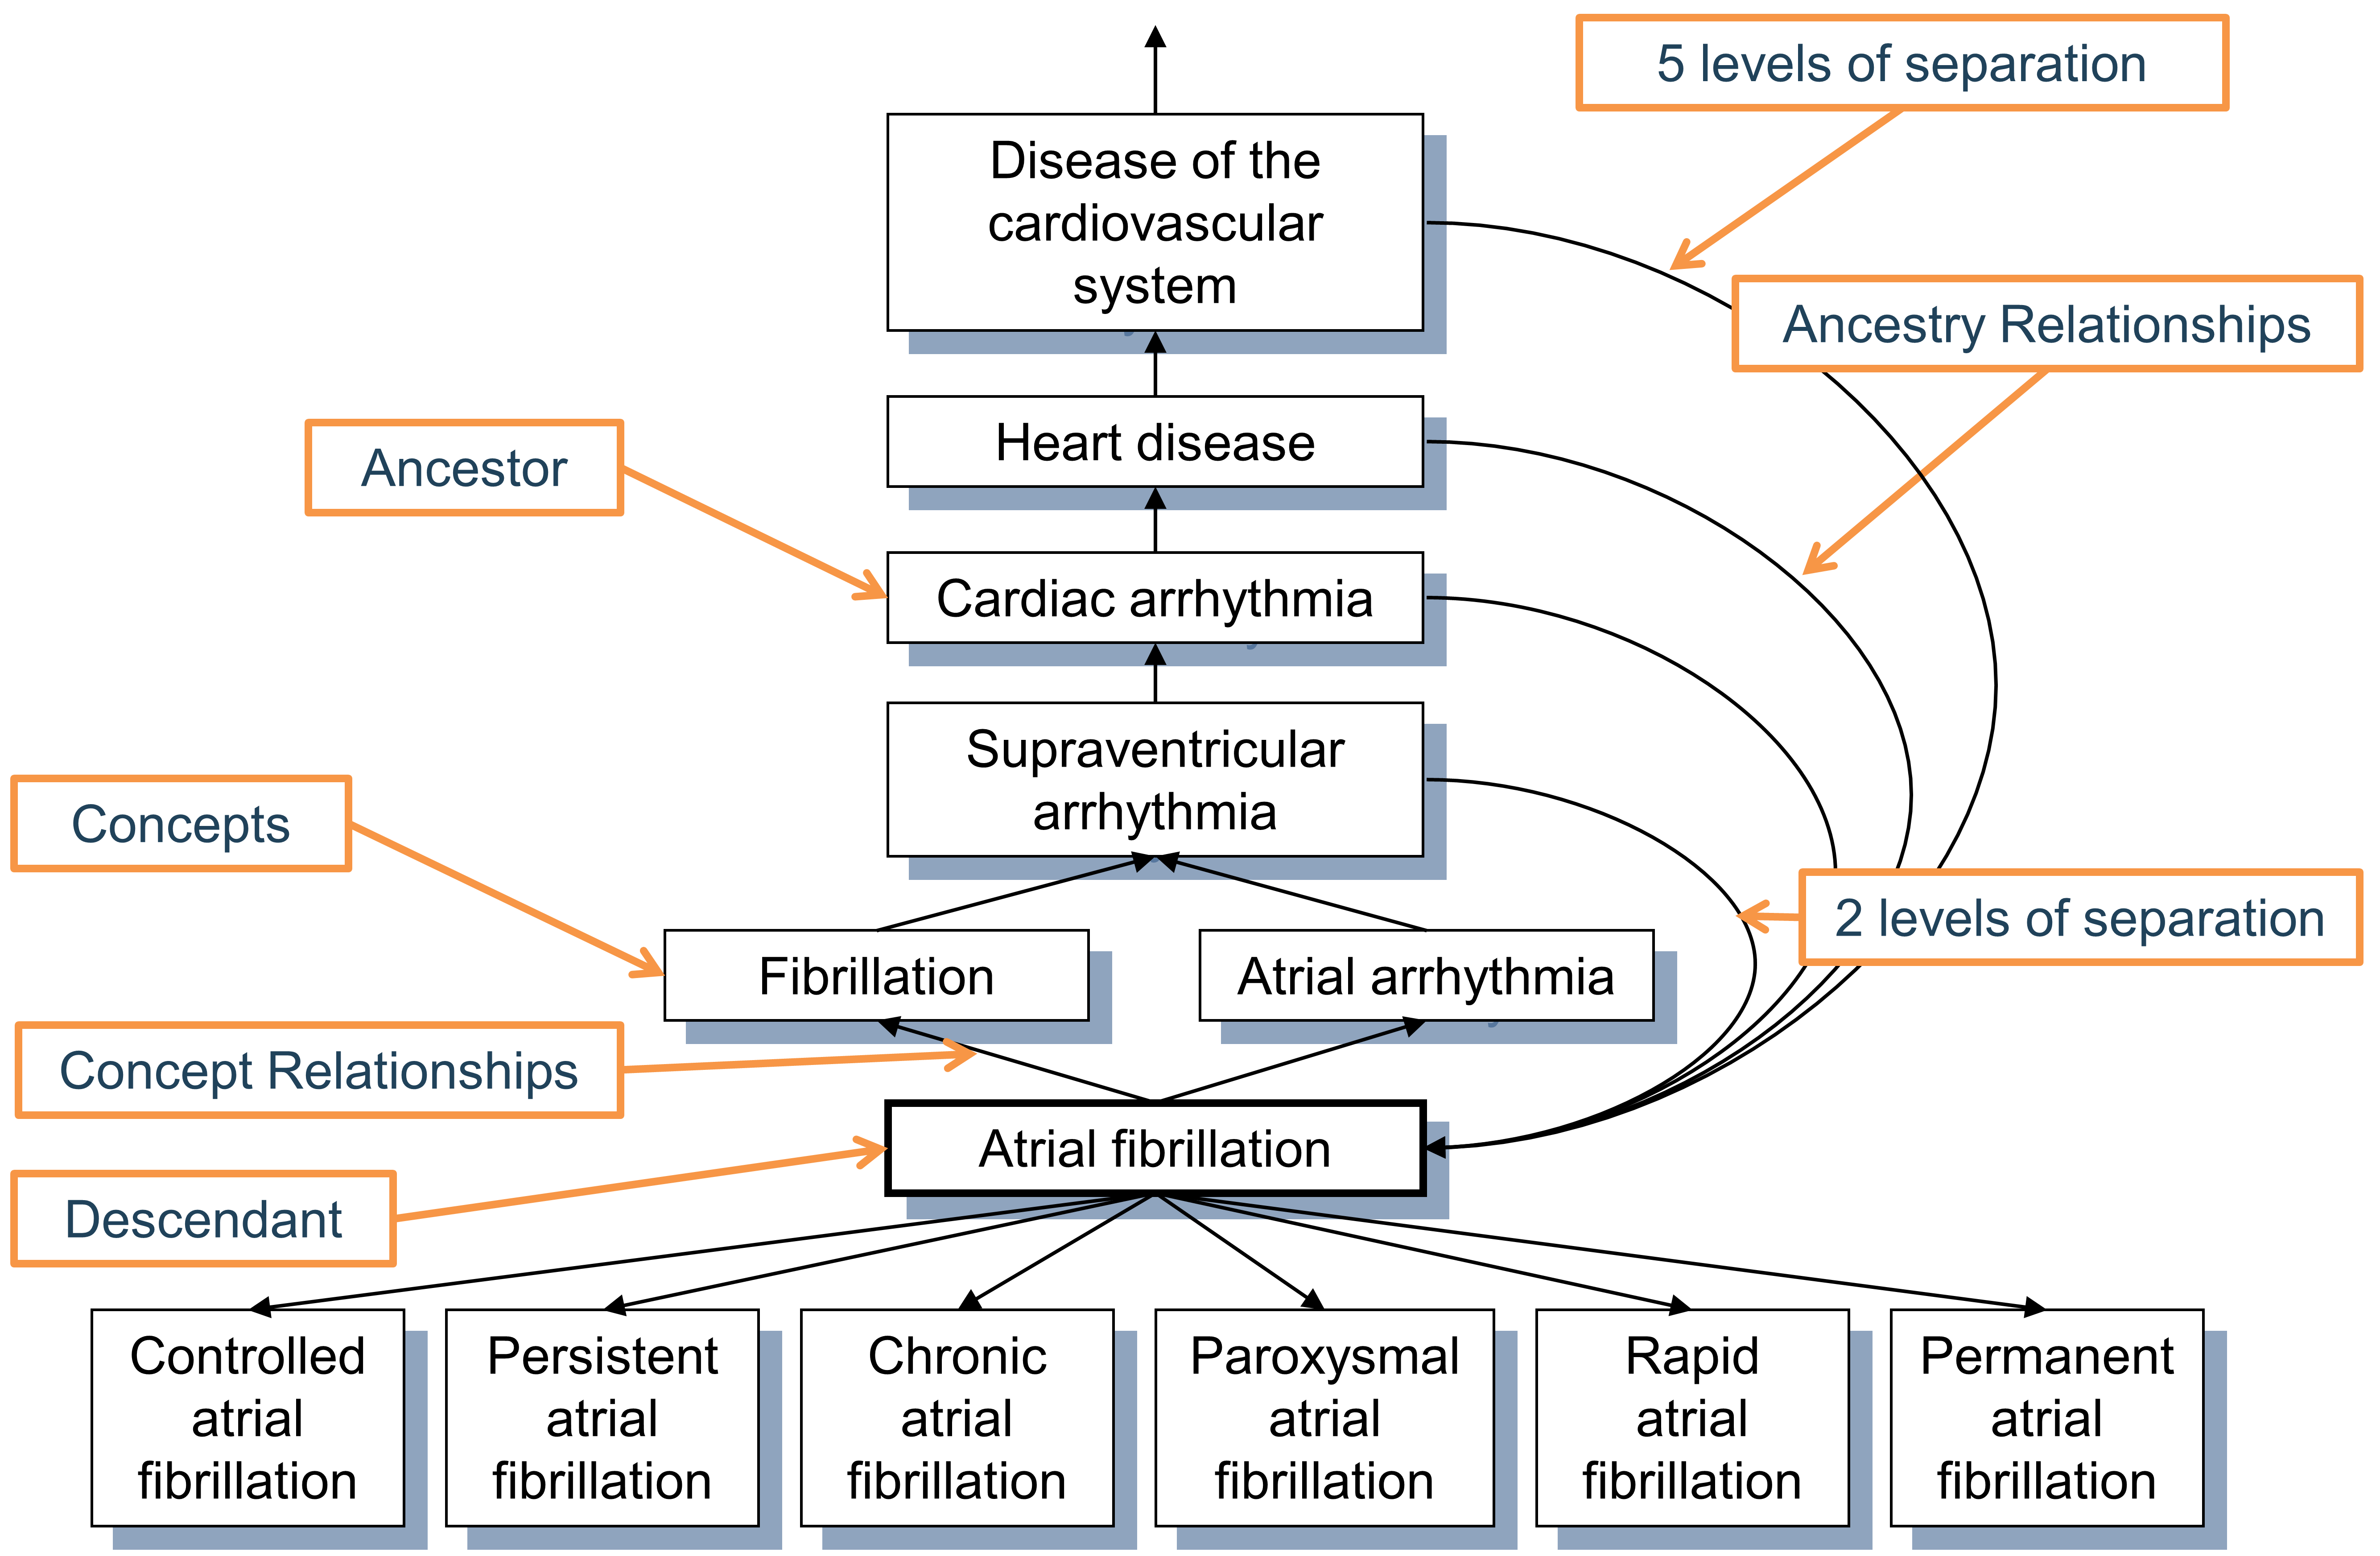
\includegraphics[width=1\linewidth]{images/StandardizedVocabularies/conceptAncestor} 

}

\caption{「心房細動」という条件の階層。第一度の先祖関係は「Is a」と「Subsumes」関係によって定義され、それより高次の関係はすべて推論され、CONCEPT\_ANCESTORテーブルに格納されます。各コンセプトは、それぞれ自身の直系の子孫でもあり、両方の分離レベルは0です。 \index{コンセプト!祖先}}\label{fig:conceptAncestor}
\end{figure}

祖先の度合い、つまり祖先と子孫の間のステップ数は、MIN\_LEVELS\_OF\_SEPARATIONおよびMAX\_LEVELS\_OF\_SEPARATIONフィールドに記録され、最短または最長の接続を定義します。すべての階層関係が分離レベルの計算に等しく寄与するわけではありません。この度合いにカウントされるステップは、各関係IDに対してRELATIONSHIP参照テーブルのIS\_HIERARCHICALフラグによって決まります。

現辞典では、高品質で包括的な階層は薬剤とコンディションの2つのドメインにのみ存在します。処置、測定値、および観察のドメインは部分的にしかカバーされておらず、構築中です。祖先関係は、原産国、ブランド名、その他の属性に関係なく、指定された成分や薬効分類のすべての薬品を参照できるため、「薬」のドメインでは特に有用です。

\section{内部参照テーブル}\label{ux5185ux90e8ux53c2ux7167ux30c6ux30fcux30d6ux30eb}

DOMAIN\_ID、VOCABULARY\_ID、CONCEPT\_CLASS\_ID(すべてCONCEPTレコード内)およびCONCEPT\_RELATIONSHIP\_ID(CONCEPT\_RELATIONSHIP内)は、すべて独自の語彙によって制御されています。これらは、4つの参照テーブル DOMAIN、VOCABULARY、CONCEPT\_CLASS、RELATIONSHIP で定義されており、*\_ID フィールドを主キーとして、より詳細な *\_NAME フィールドと、CONCEPT テーブルへの参照を持つ *\_CONCEPT\_ID フィールドを含んでいます。CONCEPT テーブルには、参照テーブルのレコードそれぞれに対応するコンセプトが含まれています。これらの重複レコードの目的は、自動ナビゲーションエンジンを可能にする情報モデルをサポートすることです。 また、VOCABULARYテーブルには、オリジナルのボキャブラリソースとバージョンを参照するVOCABULARY\_REFERENCEとVOCABULARY\_VERSIONフィールドが含まれています。RELATIONSHIPテーブルには、追加のフィールドとしてDEFINES\_ANCESTRY、IS\_HIERARCHICAL、REVERSE\_RELATIONSHIP\_IDがあります。後者は、関係のペアのカウンター関係IDを定義します。

\section{特別な状況}\label{specialSituations}

\subsection{性別}\label{ux6027ux5225}

OMOP CDMと標準化ボキャブラリにおける性別は、出生時の生物学的性別を意味します。代替の性別をどのように定義するのかという質問がよく寄せられます。 このようなケースは、OBSERVATION テーブルのレコードでカバーする必要があります。このテーブルには、本人が定義した性別が格納されます(データ資産にそのような情報が含まれている場合)。

\subsection{人種と民族}\label{ux4ebaux7a2eux3068ux6c11ux65cf}

これらは米国政府の定義に従います。民族はヒスパニック系または非ヒスパニック系の区別であり、人種は問いません。人種は一般的な上位5つの人種に分けられ、民族は階層的な子孫として含まれます。混血はは含まれていません。

\subsection{診断コーディングシステムとOMOP条件}\label{ux8a3aux65adux30b3ux30fcux30c7ux30a3ux30f3ux30b0ux30b7ux30b9ux30c6ux30e0ux3068omopux6761ux4ef6}

ICD-9やICD-10などの一般に使用されているコーディング体系は、適切な診断評価に基づいて、ある程度明確な診断を定義しています。 コンディションドメインは、このセマンティックスペースと完全に一致するものではありませんが、部分的に重複しています。 例えば、コンディションには診断が下される前に記録される徴候や症状も含まれます。また、ICDコードには他のドメイン(例えば、処置)に属するコンセプトも含まれます。

\subsection{処置コードシステム}\label{ux51e6ux7f6eux30b3ux30fcux30c9ux30b7ux30b9ux30c6ux30e0}

同様に、HCPCSやCPT4のようなコーディングシステムは医療処置のリストであると考えられます。実際には、これらは医療サービスに対する支払い請求の根拠となるメニューのようなものです。これらのサービスの多くは処置ドメインに含まれますが、多くのコンセプトはこれに該当しません。

\subsection{医療機器}\label{ux533bux7642ux6a5fux5668}

医療機器のコンセプトには、標準コンセプトのソースとして使用できる標準化されたコーディングスキームがありません。多くのソースデータでは、医療機器はコード化されていないか、外部のコーディングスキームにも含まれていません。同じ理由により、現在利用可能な階層システムはありません。

\subsection{ビジットとサービス}\label{ux30d3ux30b8ux30c3ux30c8ux3068ux30b5ux30fcux30d3ux30b9}

ビジットのコンセプトは、医療受診の性質を定義します。多くのソースシステムでは、これらはサービス提供場所として呼ばれており、病院などの組織や物理的構造を示します。他のソースシステムでは、サービスと呼ばれます。これらの用語の定義も国によって異なり、その定義を入手するのは困難です。医療施設は、数少ない訪問の1つに特化していることが多い(XYZ病院)ですが、それでもそれらによって定義されるべきではありません(XYZ病院でも、患者は病院外のビジットをすることがある)。

\subsection{医療提供者と専門分野}\label{ux533bux7642ux63d0ux4f9bux8005ux3068ux5c02ux9580ux5206ux91ce}

医療提供者は、医療提供者ドメインで定義されます。これには、医師や看護師などの医療専門家だけでなく、検眼医や靴職人などの医療以外の専門家も含まれます。専門分野は、医療提供者「医師」の子孫です。医療施設は専門分野を持つことはできませんが、主要スタッフの専門分野で定義されることはよくあります(「外科」など)。

\subsection{特別な要件を持つ治療領域}\label{ux7279ux5225ux306aux8981ux4ef6ux3092ux6301ux3064ux6cbbux7642ux9818ux57df}

標準化ボキャブラリは包括的に医療のあらゆる側面をカバーしています。しかし、一部の治療領域では特別なニーズがあり、特別なボキャブラリが必要となります。例としては、腫瘍学、放射線医学、ゲノミクスが挙げられます。これらの拡張を開発するために、特別なOHDSIワーキンググループが存在します。その結果、OMOPで標準化ボキャブラリは、異なる起源と目的を持つコンセプトがすべて同じドメイン固有の階層に存在する統合システムを構成しています。

\subsection{薬剤ドメインにおける標準コンセプト}\label{rxNormExtension}

薬剤ドメインの多くのコンセプトは、米国国立医学図書館が作成した公的に利用可能なボキャブラリであるRxNormから引用されています。ただし、米国外の医薬品については、成分、形態、および強度の組み合わせが米国で市販されているかどうかに応じて、対象とならない場合があります。米国市場にない医薬品は、OHDSIボキャブラリチームによって、唯一の大規模ドメインボキャブラリである\href{https://www.ohdsi.org/web/wiki/doku.php?id=documentation:vocabulary:rxnorm_extension}{RxNorm Extension}というボキャブラリに追加されます。

\subsection{NULLのバリエーション}\label{nullux306eux30d0ux30eaux30a8ux30fcux30b7ux30e7ux30f3}

多くのボキャブラリには、情報の欠如に関するコードが含まれています。例えば、5つの性別コンセプト8507「男性」、8532「女性」、8570「曖昧」、8551「不明」、および8521「その他」のうち、標準コンセプトは最初の2つのみであり、他の3つはマッピングなしのソースコンセプトです。標準化ボキャブラリでは、なぜ情報が利用できないかの区別はなされません。それは患者による情報の積極的な撤回、欠落値、何らかの形で定義または標準化されていない値、またはCONCEPT\_RELATIONSHIPでのマッピング記録の欠如によるものである可能性があります。このようなコンセプトはマッピングされず、標準コンセプトのコンセプトID=0のデフォルトマッピングに対応します。

\section{まとめ}\label{ux307eux3068ux3081-3}

\begin{rmdsummary}
\begin{itemize}
\tightlist
\item
  すべてのイベントと管理上の事実は、OMOP標準化ボキャブラリでコンセプト、コンセプト関係、コンセプト祖先階層として表されます。
\item
  これらのほとんどは既存のコーディングスキームやボキャブラリから採用されていますが、一部はOHDSIボキャブラリチームによって新規にキュレーションされます。
\item
  すべてのコンセプトにはドメインが割り当てられ、そのコンセプトが表す事象がCDMのどこに格納されるかが制御されます。
\item
  異なるボキャブラリにおける同等の意味を持つコンセプトは、そのうちの1つにマッピングされ、これが標準コンセプトとして指定されます。その他のコンセプトはソースコンセプトです。
\item
  マッピングは「Maps to」および「Maps to value」というコンセプト関係を通じて行われます。
\item
  分類コンセプトという追加のコンセプトクラスがあり、これらは非標準ですが、ソースコンセプトとは異なり、階層構造に参加します。
\item
  コンセプトには時間の経過とともにライフサイクルがあります。
\item
  ドメイン内のコンセプトは階層に整理されています。階層の質はドメインごとに異なり、階層システムの完成は継続的な作業です。
\item
  間違いや不正確さを発見した場合は、コミュニティに積極的に参加することを強くお勧めします。
\end{itemize}
\end{rmdsummary}

\section{演習}\label{ux6f14ux7fd2-1}

\subsubsection*{前提条件}\label{ux524dux63d0ux6761ux4ef6-2}
\addcontentsline{toc}{subsubsection}{前提条件}

最初の演習では、標準化ボキャブラリのコンセプトを検索する必要があります。これはATHENA\footnote{\url{http://athena.ohdsi.org/}}またはATLAS\footnote{\url{http://atlas-demo.ohdsi.org}}を通じて行うことができます。

\begin{exercise}
\protect\hypertarget{exr:exerciseVocab1}{}\label{exr:exerciseVocab1}``消化管出血''の標準コンセプトIDは何ですか?
\end{exercise}

\begin{exercise}
\protect\hypertarget{exr:exerciseVocab2}{}\label{exr:exerciseVocab2}``消化管出血''の標準コンセプトに対応するICD-10CMコードは何ですか?この標準コンセプトに対応するICD-9CMコードはどれですか?
\end{exercise}

\begin{exercise}
\protect\hypertarget{exr:exerciseVocab3}{}\label{exr:exerciseVocab3}``消化管出血''の標準コンセプトに相当するMedDRAの優先用語は何ですか?
\end{exercise}

回答例は付録 \ref{Vocabanswers}を参照のこと。

\chapter{--翻訳作業中-- 抽出、変換、ロード}\label{ExtractTransformLoad}

\emph{章の著者: Clair Blacketer \& Erica Voss}

\section{はじめに}\label{ux306fux3058ux3081ux306b}

ネイティブ/生データからOMOP共通データモデル(CDM)を作成するには、抽出、変換、ロード(ETL)プロセスを作成する必要があります。このプロセスでは、データをCDMに再構築し、標準化ボキャブラリにマッピングを追加する必要があります。通常、このプロセスは、例えばSQLスクリプトのような自動化されたスクリプトのセットとして実装されます。このETLプロセスは繰り返し実行できることが重要です。これにより、ソースデータが更新されるたびに再実行することができます。\index{ETL|see {抽出、変換、ロード(ETL)}} \index{生データ} \index{ネイティブデータ|see {生データ}} \index{ソースデータ|see {生データ}}

ETLの作成は通常、大規模な取り組みとなります。長年にわたり、私たちは以下の4つの主要なステップからなるベストプラクティスを開発してきました:

\begin{enumerate}
\def\labelenumi{\arabic{enumi}.}
\tightlist
\item
  データの専門家とCDMの専門家が共同でETLをデザインする。
\item
  医学的知識を持つ人がコードのマッピングをする。
\item
  技術者がETLを実装する。
\item
  全員が品質管理に関与する。
\end{enumerate}

本章では、これらのステップをそれぞれ詳しく説明します。OHDSIコミュニティでは、これらのステップの一部をサポートするツールがいくつか開発されており、それらについても説明します。本章の最後に、CDMとETLのメンテナンスについて説明します。

\section{ステップ 1: ETLのデザイン}\label{ux30b9ux30c6ux30c3ux30d7-1-etlux306eux30c7ux30b6ux30a4ux30f3}

ETLのデザインと実装を明確に区別することが重要です。ETLのデザインにはソースデータとCDMの両方に関する広範な知識が必要です。一方、ETLの実装は通常、ETLを計算効率的に行うための技術的専門知識に大きく依存します。両方を同時に行おうとすると、細部にこだわってしまい、全体像に集中できなくなることがあります。

ETLデザインプロセスを支援するために密接に統合された2つのツールが開発されました:White RabbitとRabbit-in-a-Hatです。

\subsection{White Rabbit}\label{white-rabbit}

データベースでETLプロセスを開始するには、データ(テーブル、フィールド、内容など)を理解する必要があります。そこで登場するのが\href{https://github.com/OHDSI/WhiteRabbit}{White Rabbit}ツールです。White Rabbitは、縦断的な医療データベースのETLを\href{https://github.com/OHDSI/CommonDataModel}{OMOP CDM}用に準備するためのソフトウェアツールです。White Rabbitはデータをスキャンし、ETLのデザインを開始するために必要なすべての情報を含むレポートを作成します。全てのソースコードとインストール手順、マニュアルへのリンクはGitHubで入手可能です\footnote{\url{https://github.com/OHDSI/WhiteRabbit}.}。\index{White Rabbit} \index{data profiling|see {White Rabbit}}

\subsubsection*{範囲と目的}\label{ux7bc4ux56f2ux3068ux76eeux7684}
\addcontentsline{toc}{subsubsection}{範囲と目的}

White Rabbitの主な機能は、ソースデータをスキャンし、テーブル、フィールド、フィールドに表示される値に関する詳細な情報を提供することです。ソースデータは、カンマ区切りのテキストファイルやデータベース(MySQL、SQL Server、Oracle、PostgreSQL、Microsoft APS、Microsoft Access、Amazon Redshift)に保存される必要があります。スキャンによって、例えばRabbit-In-a-Hatツールと併用して、ETLデザイン時に参照用として使用できるレポートが作成されます。White Rabbitは標準的なデータプロファイリングツールとは異なり、生成された出力データファイルに個人識別情報(PII)を表示しないようにします。

\subsubsection*{プロセス概要}\label{ux30d7ux30edux30bbux30b9ux6982ux8981}
\addcontentsline{toc}{subsubsection}{プロセス概要}

ソフトウェアを使用してソースデータをスキャンする一般的な手順は以下の通りです:

\begin{enumerate}
\def\labelenumi{\arabic{enumi}.}
\tightlist
\item
  作業フォルダを設定します。作業フォルダは、結果がエクスポートされるローカルのデスクトップコンピュータ上の場所です。
\item
  ソースデータベースまたはCSVテキストファイルに接続し、接続をテストします。
\item
  スキャン対象のテーブルを選択し、テーブルをスキャンします。
\item
  White Rabbitがソースデータに関する情報をエクスポートします。
\end{enumerate}

\subsubsection*{作業フォルダの設定}\label{ux4f5cux696dux30d5ux30a9ux30ebux30c0ux306eux8a2dux5b9a}
\addcontentsline{toc}{subsubsection}{作業フォルダの設定}

White Rabbitアプリケーションをダウンロードしてインストールした後、まず最初に作業フォルダを設定する必要があります。White Rabbitが作成するすべてのファイルはこのローカルフォルダにエクスポートされます。図\ref{fig:WhiteRabbitLocation}に示されている「Pick Folder(フォルダの選択)」ボタンを使用して、スキャン文書を保存するローカル環境をナビゲートします。

\begin{figure}

{\centering 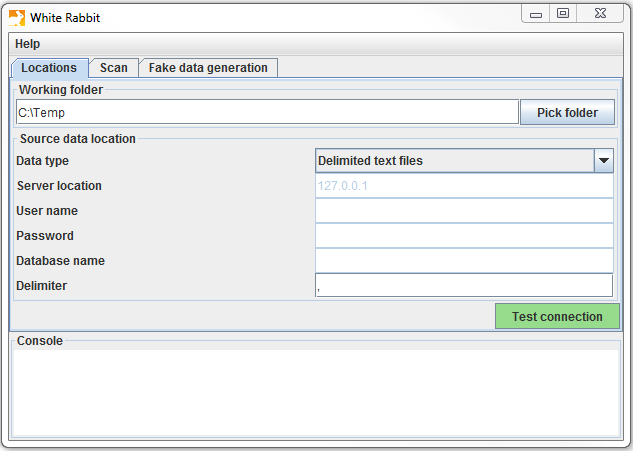
\includegraphics[width=1\linewidth]{images/ExtractTransformLoad/WhiteRabbitLocation} 

}

\caption{White Rabbitアプリケーションの作業フォルダを指定するための「Pick Folder」ボタン}\label{fig:WhiteRabbitLocation}
\end{figure}

\subsubsection*{データベースへの接続}\label{ux30c7ux30fcux30bfux30d9ux30fcux30b9ux3078ux306eux63a5ux7d9a}
\addcontentsline{toc}{subsubsection}{データベースへの接続}

White Rabbitは区切りテキストファイルとさまざまなデータベースプラットフォームをサポートしています。各フィールドにマウスカーソルを合わせると、必要な情報が表示されます。詳細についてはマニュアルをご覧ください。

\subsubsection*{データベース内のテーブルをスキャン}\label{ux30c7ux30fcux30bfux30d9ux30fcux30b9ux5185ux306eux30c6ux30fcux30d6ux30ebux3092ux30b9ux30adux30e3ux30f3}
\addcontentsline{toc}{subsubsection}{データベース内のテーブルをスキャン}

データベースに接続後、含まれるテーブルをスキャンできます。スキャンによりETLのデザインに役立つ情報を含むレポートが生成されます。図\ref{fig:WhiteRabbitAddTables}に示されたスキャンタブを使用して、「Add」(Ctrl + マウスクリック)をクリックして選択したソースデータベース内の個々のテーブルを選択するか、データベース内のすべてのテーブルを自動的に選択する「Add all in DB」ボタンをクリックできます。

\begin{figure}

{\centering 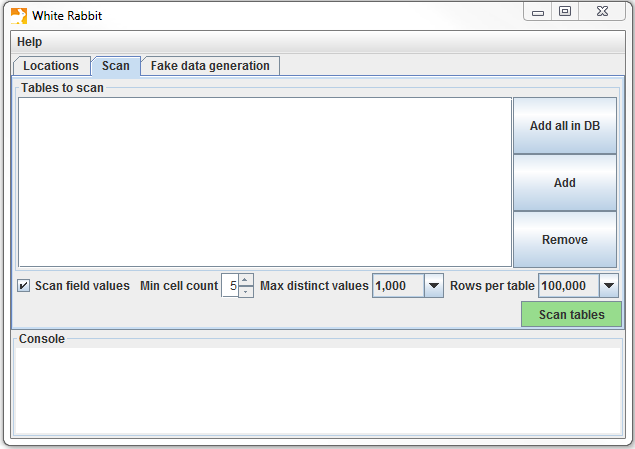
\includegraphics[width=1\linewidth]{images/ExtractTransformLoad/WhiteRabbitAddTables} 

}

\caption{White Rabbit スキャンタブ}\label{fig:WhiteRabbitAddTables}
\end{figure}

スキャンにはいくつかの設定オプションもあります:

\begin{itemize}
\tightlist
\item
  「フィールド値をスキャン」をチェックすると、列に表示される値を調査したいことを WhiteRabbit に通知します。
\item
  「最小セル数」はフィールド値のスキャン時のオプションです。デフォルトでは5に設定されており、ソースデータで5回未満しか表示されない値は報告に表示されません。個別のデータセットには、この最小セル数に関する独自のルールがある場合があります。
\item
  「テーブルあたりの行数」はフィールド値のスキャン時のオプションです。デフォルトでは、White Rabbitはテーブル内の100,000行をランダムに選択してスキャンします。
\end{itemize}

すべての設定が完了したら、「テーブルをスキャン」ボタンをクリックします。スキャンが完了すると、レポートが作業フォルダに書き込まれます。

\subsubsection*{スキャンレポートの解釈}\label{ux30b9ux30adux30e3ux30f3ux30ecux30ddux30fcux30c8ux306eux89e3ux91c8}
\addcontentsline{toc}{subsubsection}{スキャンレポートの解釈}

スキャンが完了すると、選択したフォルダにスキャンしたテーブルごとにタブが設けられたExcelファイルが作成されます。 また、概要タブも用意されています。 概要タブには、スキャンしたすべてのテーブル、各テーブルの各フィールド、各フィールドのデータタイプ、フィールドの最大長、テーブルの行数、スキャンした行数、各フィールドが空欄であることが判明した頻度が記載されています。図\ref{fig:ScanOverviewTab}.は、概要タブの例を示しています。

\begin{figure}

{\centering 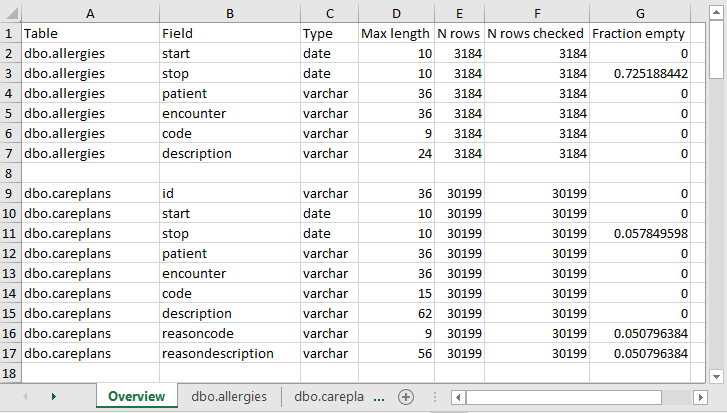
\includegraphics[width=1\linewidth]{images/ExtractTransformLoad/ScanOverviewTab} 

}

\caption{スキャンレポートのサンプル概要タブ}\label{fig:ScanOverviewTab}
\end{figure}

各テーブルのタブには、各フィールド、各フィールド内の値、各値の頻度が示されます。各ソーステーブルの列は、Excelに2つの列を生成します。1つの列には、「最小セルカウント」がスキャン時に設定された値よりも大きいすべての異なる値がリストされます。一意の値のリストが切り捨てられた場合、リストの最後の値は「リストが切り捨てられました」となります。これは、「最小セルカウント」に入力された数値よりも少ない数の追加の一意のソース値が1つ以上存在することを示します。各一意の値の隣には、2番目の列として頻度(サンプルに含まれるその値の回数)が表示されます。この2つの列(一意の値と頻度)は、ワークブックでプロファイルされたテーブル内のすべてのソース列に対して繰り返されます。

\begin{figure}

{\centering 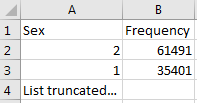
\includegraphics[width=0.3\linewidth]{images/ExtractTransformLoad/ScanSex} 

}

\caption{単一列のサンプル値}\label{fig:scanSex}
\end{figure}

レポートはソースデータを理解するのに強力であり、存在するものを強調して表示します。例えば、図\ref{fig:scanSex}に示された結果がスキャンされたテーブルの「Sex」列に戻された場合、2つの共通値(1と2)がそれぞれ61,491回と35,401回出現したことが分かります。White Rabbitは1を男性、2を女性として定義することはなく、データホルダーが通常、ソースシステムに固有のソースコードを定義する必要があります。しかし、このリストが切り捨てられていることから、データにはこの2つの値(1と2)だけが存在しているわけではないことが分かります。これらの他の値は、「最小セル数」で定義されるように、非常に低い頻度でしか現れず、不正確な値や非常に疑わしい値であることがよくあります。ETLを生成する際には、高頻度の性別コンセプト1と2だけでなく、この列に存在するその他の頻度の低い値も処理できるように計画する必要があります。例えば、低頻度の性別が「NULL」であった場合、ETLがそのデータを処理でき、その状況で何をすべきかを知っていることを確認する必要があります。

\subsection{Rabbit-In-a-Hat}\label{rabbit-in-a-hat}

White Rabbitスキャンを手にすると、ソースデータの全体像やCDMの仕様が掴めます。次に、これら2つの間の論理を定義する必要があります。この設計作業には、ソースデータとCDMの両方に関する深い知識が必要です。White Rabbitソフトウェアと共に提供されるRabbit-in-a-Hatツールは、これらの分野の専門家チームをサポートするように特別にデザインされています。典型的な設定では、ETL設計チームが一堂に会し、Rabbit-in-a-Hatをスクリーンに映し出します。最初のラウンドでは、テーブル間のマッピングを共同で決定し、その後、フィールド間のマッピングを設計し、値が変換されるロジックを定義します。\index{Rabbit-In-A-Hat} \index{ETL design|see {Rabbit-In-A-Hat}}

\subsubsection*{範囲と目的}\label{ux7bc4ux56f2ux3068ux76eeux7684-1}
\addcontentsline{toc}{subsubsection}{範囲と目的}

Rabbit-In-a-HatはWhite Rabbitのスキャン文書を読み取り、表示するように設計されています。White Rabbitはソースデータに関する情報を生成し、Rabbit-In-a-Hatはその情報を使用して、グラフィカルユーザーインターフェイスを通じて、ユーザーがソースデータをCDMのテーブルとカラムに接続できるようにします。Rabbit-In-a-HatはETLプロセスのドキュメントを生成しますが、ETLを作成するコードは生成しません。

\subsubsection*{プロセス概要}\label{ux30d7ux30edux30bbux30b9ux6982ux8981-1}
\addcontentsline{toc}{subsubsection}{プロセス概要}

このソフトウェアを使用してETLのドキュメントを生成する一般的な手順は以下の通りです:

\begin{enumerate}
\def\labelenumi{\arabic{enumi}.}
\tightlist
\item
  White Rabbitのスキャン結果を完了させます。
\item
  スキャン結果を開くと、インターフェースにソーステーブルとCDMテーブルが表示されます。
\item
  ソーステーブルが対応するCDMテーブルに情報を提供する場合は、ソーステーブルをCDMテーブルに接続します。
\item
  各ソーステーブルからCDMテーブルへの接続について、ソース列とCDM列の詳細でさらに定義します。
\item
  Rabbit-In-a-Hatの作業内容を保存し、MS Word文書にエクスポートします。
\end{enumerate}

\subsubsection*{ETLロジックの記述}\label{etlux30edux30b8ux30c3ux30afux306eux8a18ux8ff0}
\addcontentsline{toc}{subsubsection}{ETLロジックの記述}

White RabbitスキャンレポートをRabbit-In-a-Hatで開くと、ソースデータをOMOP CDMに変換する方法のロジックの設計と記述する準備が整ったことになります。次のセクションでは、Synthea\footnote{Synthea\textsuperscript{TM}は実際の患者をモデル化することを目的とした患者ジェネレーターです。データはアプリケーションに渡されたパラメータに基づいて作成されます。データの構造については、こちら:\url{https://github.com/synthetichealth/synthea/wiki} をご覧ください。}データベースのいくつかのテーブルが変換中にどのように見えるかを例示します。

\subsubsection*{ETLの一般的なフロー}\label{etlux306eux4e00ux822cux7684ux306aux30d5ux30edux30fc}
\addcontentsline{toc}{subsubsection}{ETLの一般的なフロー}

CDMは人を中心としたモデルであるため、PERSONテーブルのマッピングを最初に始めることが常に良い方法です。すべての臨床イベントテーブル(CONDITION\_OCCURRENCE、DRUG\_EXPOSURE、PROCEDURE\_OCCURRENCEなど)は、person\_idを介してPERSONテーブルを参照するため、最初にPERSONテーブルのロジックを構築しておくと、後で作業が容易になります。PERSONテーブルの次に、OBSERVATION\_PERIODテーブルを変換するのが良い方法です。CDMデータベースの各人には少なくとも1つのOBSERVATION\_PERIODがあり、通常、ほとんどのイベントはこの期間内に発生します。PERSONテーブルとOBSERVATION\_PERIODテーブルが完了したら、次にPROVIDER、CARE\_SITE、LOCATIONなどのディメンショナルテーブルが通常は続きます。臨床テーブルの前に作成すべき最後のテーブルロジックはVISIT\_OCCURRENCEです。これはETL全体で最も複雑なロジックであることが多くまた、患者の旅の過程で発生するほとんどのイベントは来院時に発生するため、最も重要なものの1つです。これらのテーブルが完了したら、どのCDMテーブルをどのような順序でマッピングするかは実施者の選択にゆだねられます。

\begin{figure}

{\centering 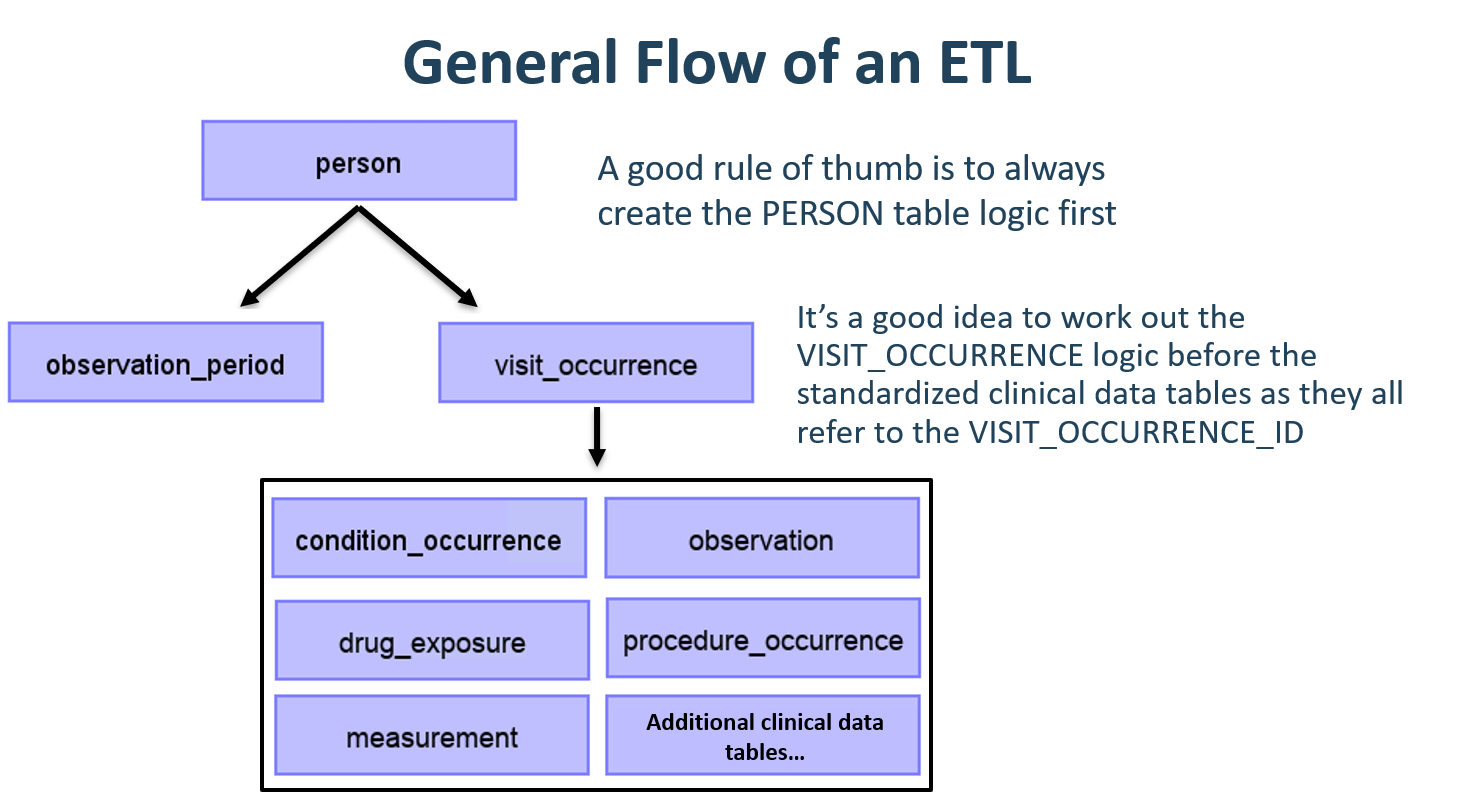
\includegraphics[width=1\linewidth]{images/ExtractTransformLoad/flowOfEtl} 

}

\caption{ETLの一般的なフローと、最初にマッピングするテーブル}\label{fig:etlFlow}
\end{figure}

CDM変換中に中間テーブルの作成が必要になることがよくあります。これは、イベントに正しいVISIT\_OCCURRENCE\_IDを割り当てるため、またはソースコードを標準コンセプトにマッピングするためです(このステップをその場で実行すると非常に時間がかかることがよくあります)。中間テーブルは100%許可され推奨されています。ただし、変換が完了した後にこれらの中間テーブルを永続的に使用し続け、それらに依存することは推奨されません。

\subsubsection*{マッピング例:Personテーブル}\label{ux30deux30c3ux30d4ux30f3ux30b0ux4f8bpersonux30c6ux30fcux30d6ux30eb}
\addcontentsline{toc}{subsubsection}{マッピング例:Personテーブル}

Syntheaデータ構造にはpatientsテーブルに20のカラムがありますが、図\ref{fig:syntheaPerson} に示されているように、すべてがPERSONテーブルを埋めるために必要というわけではありません。これは非常に一般的であり、心配する必要はありません。この例では、CDM PERSONテーブルで使用されていないSynthea patientsテーブルのデータポイントの多くは患者名、運転免許証番号、パスポート番号などの追加識別子です。

\begin{figure}

{\centering 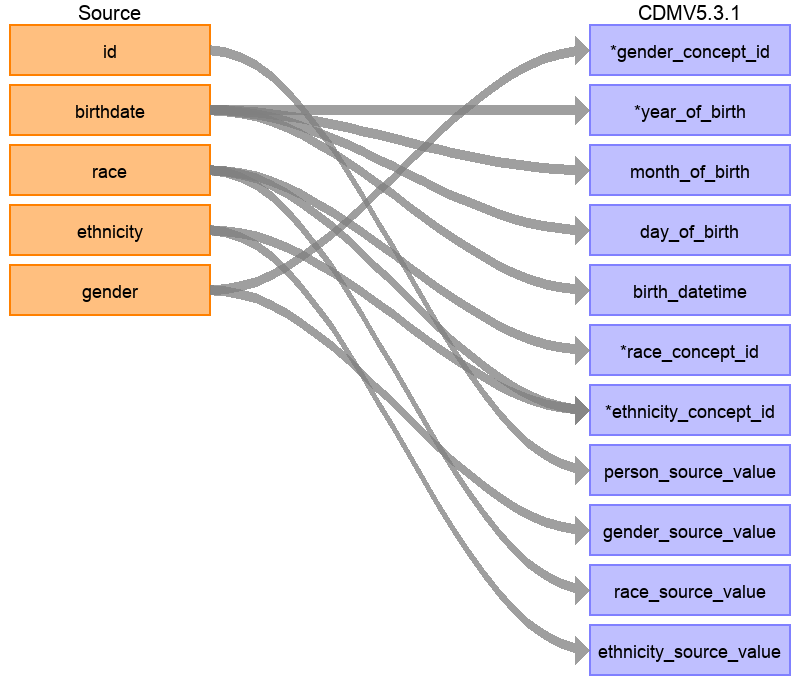
\includegraphics[width=1\linewidth]{images/ExtractTransformLoad/syntheaPersonTable} 

}

\caption{Synthea PatientsテーブルからCDM PERSONテーブルへのマッピング}\label{fig:syntheaPerson}
\end{figure}

表 \ref{tab:syntheaEtlPerson} には、Synthea patientsテーブルをCDM PERSONテーブルに変換するために適用されたロジックを示しています。『Destination Field』(変換先フィールド)は、CDMのどこにデータがマッピングされるかを示しています。『Source field』(変換元フィールド)では、CDMカラムにデータを入力するのに使用されるソーステーブル(この場合はpatients)のカラムを強調して表示しています。最後に、『Logic \& comments』(ロジックとコメント)カラムには、ロジックの説明が記載されています。

\begin{longtable}[]{@{}
  >{\raggedright\arraybackslash}p{(\columnwidth - 4\tabcolsep) * \real{0.3333}}
  >{\raggedright\arraybackslash}p{(\columnwidth - 4\tabcolsep) * \real{0.3333}}
  >{\raggedright\arraybackslash}p{(\columnwidth - 4\tabcolsep) * \real{0.3333}}@{}}
\caption{\label{tab:syntheaEtlPerson} Synthea PatientsテーブルをCDM PERSONテーブルに変換するためのETLロジック}\tabularnewline
\toprule\noalign{}
\begin{minipage}[b]{\linewidth}\raggedright
目的フィールド
\end{minipage} & \begin{minipage}[b]{\linewidth}\raggedright
ソースフィールド
\end{minipage} & \begin{minipage}[b]{\linewidth}\raggedright
ロジックとコメント
\end{minipage} \\
\midrule\noalign{}
\endfirsthead
\toprule\noalign{}
\begin{minipage}[b]{\linewidth}\raggedright
目的フィールド
\end{minipage} & \begin{minipage}[b]{\linewidth}\raggedright
ソースフィールド
\end{minipage} & \begin{minipage}[b]{\linewidth}\raggedright
ロジックとコメント
\end{minipage} \\
\midrule\noalign{}
\endhead
\bottomrule\noalign{}
\endlastfoot
PERSON\_ID & & 自動生成。 PERSON\_IDは実装時に生成されます。これは、ソースのid値がvarchar値であるのに対し、PERSON\_IDは整数であるためです。 ソースからのidフィールドは、その値を保持し、必要に応じてエラーチェックを行うためにPERSON\_SOURCE\_VALUEとして設定されます。 \\
GENDER\_CONCEPT\_ID & gender & 性別が「M」の場合、GENDER\_CONCEPT\_IDは8507、性別が「F」の場合は8532に設定します。性別不明の行は削除します。これらの2つのコンセプトは、性別ドメインの唯一の標準コンセプトであるため選択されました。性別不明の患者を削除するかどうかの決定は、通常、施設で行われる傾向がありますが、性別不明の人は分析から除外されるため、削除することが推奨されます。 \\
YEAR\_OF\_BIRTH & birthdate & 生年月日から年を取得します。 \\
MONTH\_OF\_BIRTH & birthdate & 生年月日から月を取得します。 \\
DAY\_OF\_BIRTH & birthdate & 生年月日から日を取得します。 \\
BIRTH\_DATETIME & birthdate & 0時を00:00:00とします。ここでは、ソースが出生時間を指定していないため、深夜を出生時間として設定しました。 \\
RACE\_CONCEPT\_ID & race & race = 'WHITE'の場合は8527、race = 'BLACK'の場合は8516、race = 'ASIAN'の場合は8515、それ以外の場合は0として設定します。これらのコンセプトが選択されたのは、人種ドメインに属する標準コンセプトであり、ソース内の民族カテゴリーに最も近いためです。 \\
ETHNICITY\_ CONCEPT\_ID & race ethnicity & race = `HISPANIC'、または民族が (`CENTRAL\_AMERICAN'、`DOMINICAN'、`MEXICAN'、`PUERTO\_RICAN'、`SOUTH\_AMERICAN') の場合、38003563 と設定し、それ以外の場合は 0 に設定します。これは、複数のソース列が 1 つの CDM 列にどのように影響するかを示す良い例です。CDM では、民族は ヒスパニックまたは非ヒスパニック として表されるため、ソース列 race とソース列ethnicityの両方の値がこの値を決定します。 \\
LOCATION\_ID & & \\
PROVIDER\_ID & & \\
CARE\_SITE\_ID & & \\
PERSON\_SOURCE\_ VALUE & id & \\
GENDER\_SOURCE\_ VALUE & gender & \\
GENDER\_SOURCE\_ CONCEPT\_ID & & \\
RACE\_SOURCE\_ VALUE & race & \\
RACE\_SOURCE\_ CONCEPT\_ID & & \\
ETHNICITY\_ SOURCE\_VALUE & ethnicity & この場合、ETHNICITY\_SOURCE\_VALUEはETHNICITY\_CONCEPT\_IDよりも詳細な値となります。 \\
ETHNICITY\_ SOURCE\_CONCEPT\_ID & & \\
\end{longtable}

SyntheaデータセットがCDMにどのようにマッピングされたかについては、仕様書全文をご覧ください\footnote{\url{https://ohdsi.github.io/ETL-Synthea/}}。

\section{ステップ2: コードマッピングの作成}\label{ux30b9ux30c6ux30c3ux30d72-ux30b3ux30fcux30c9ux30deux30c3ux30d4ux30f3ux30b0ux306eux4f5cux6210}

OMOPボキャブラリには、常にソースコードが追加されています。これは、CDMにデータを変換する際のコーディングシステムが既に含まれており、マッピングされている可能性があることを意味します。含まれているボキャブラリは、OMOPボキャブラリのVOCABULARYテーブルを確認ください。非標準のソースコード(例:ICD-10CMコード)から標準コンセプト(例:SNOMEDコード)へのマッピングを抽出するには、relationship\_id =「Maps to」を持つCONCEPT\_RELATIONSHIPテーブルのレコードを使用できます。例えば、ICD-10CMコード「I21」(「急性心筋梗塞」)の標準コンセプトIDを特定するには、次のSQLを使用します:

\begin{Shaded}
\begin{Highlighting}[]
\KeywordTok{SELECT}\NormalTok{ concept\_id\_2 }\KeywordTok{AS}\NormalTok{ standard\_concept\_id}
\KeywordTok{FROM}\NormalTok{ concept\_relationship}
\KeywordTok{INNER} \KeywordTok{JOIN}\NormalTok{ concept }\KeywordTok{AS}\NormalTok{ source\_concept}
  \KeywordTok{ON}\NormalTok{ concept\_id }\OperatorTok{=}\NormalTok{ concept\_id\_1}
\KeywordTok{WHERE}\NormalTok{ concept\_code }\OperatorTok{=} \StringTok{\textquotesingle{}I21\textquotesingle{}}
  \KeywordTok{AND}\NormalTok{ vocabulary\_id }\OperatorTok{=} \StringTok{\textquotesingle{}ICD10CM\textquotesingle{}}
  \KeywordTok{AND}\NormalTok{ relationship\_id }\OperatorTok{=} \StringTok{\textquotesingle{}Maps to\textquotesingle{}}\NormalTok{;}
\end{Highlighting}
\end{Shaded}

\begin{longtable}[]{@{}r@{}}
\toprule\noalign{}
STANDARD\_CONCEPT\_ID \\
\midrule\noalign{}
\endhead
\bottomrule\noalign{}
\endlastfoot
312327 \\
\end{longtable}

残念ながら、ソースデータがボキャブラリに含まれていないコーディングシステムを使用している場合もあります。この場合、ソースコーディングシステムから標準コンセプトへのマッピングを作成する必要があります。コードマッピングは特にソースコーディングシステムに多くのコードが含まれている場合に、困難な作業となる可能性があります。作業を用意にするために、以下の方法があります:

\begin{itemize}
\tightlist
\item
  最も頻繁に使用されるコードに焦点を当てる。使用されることのないコードや使用頻度の低いコードは、実際の研究では使用されることがないため、マッピングする価値はありません。
\item
  可能な限り既存の情報を活用しましょう。例えば、多くの国の医薬品コードはATCにマッピングされています。ATCは多くの目的に対して詳細さに欠けますが、ATCとRxNormのコンセプトの関係性を利用することで適切なRxNormコードを推測することができます。
\item
  Usagiを使用しましょう。
\end{itemize}

\subsection{Usagi}\label{usagi}

Usagiはコードマッピングを手動で作成するプロセスを支援するツールです。コードの記述のテキスト類似性に基づいて、マッピングの候補を作成することができます。ソースコードが外国語でしか利用できない場合、Google翻訳\footnote{\url{https://translate.google.com/}}は驚くほど正確な翻訳結果を提示することが多いことがわかっています。Usagiは自動提案が適切でない場合に、適切なターゲットコンセプトを検索する機能を提供します。最終的に、ユーザーはETLで使用することが承認されたマッピングを指定することができます。UsagiはGitHubで入手できます\footnote{\url{https://github.com/OHDSI/Usagi}}。 \index{Usagi} \index{source code mapping|see {Usagi}}

\subsubsection*{範囲と目的}\label{ux7bc4ux56f2ux3068ux76eeux7684-2}
\addcontentsline{toc}{subsubsection}{範囲と目的}

マッピングが必要なソースコードはUsagiに読み込みます(コードが英語でない場合は追加の翻訳列が必要です)。用語の類似性アプローチを使用してソースコードをボキャブラリコンセプトに紐づけします。ただし、これらのコードの紐づけは手動で確認する必要があり、Usagiはこれを容易にするためのインターフェースを提供します。Usagiはボキャブラリで標準コンセプトとしてマークされているコンセプトのみを提案します。

\subsubsection*{プロセス概要}\label{ux30d7ux30edux30bbux30b9ux6982ux8981-2}
\addcontentsline{toc}{subsubsection}{プロセス概要}

このソフトウェアを使用する一般的な手順は次のとおりです:

\begin{enumerate}
\def\labelenumi{\arabic{enumi}.}
\tightlist
\item
  マッピングしたいソースシステムからソースコードを読み込みます。
\item
  Usagiは用語の類似性アプローチを実行してソースコードをボキャブラリコンセプトにマッピングします。
\item
  Usagiのインターフェースを利用して、自動提案の正しさを確認し、必要に応じて改善します。コードシステムと医療用語に精通した担当者によるレビューが推奨されます。
\item
  ボキャブラリのSOURCE\_TO\_CONCEPT\_MAPにマッピングをエクスポートします。
\end{enumerate}

\subsubsection*{ソースコードをUsagiにインポート}\label{ux30bdux30fcux30b9ux30b3ux30fcux30c9ux3092usagiux306bux30a4ux30f3ux30ddux30fcux30c8}
\addcontentsline{toc}{subsubsection}{ソースコードをUsagiにインポート}

ソースコードをCSVまたはExcel (.xlsx) ファイルにエクスポートします。これには、ソースコードと英語のソースコードの説明を含む列が必要ですが、コードに追加する情報(例:用量単位、翻訳されている場合は元の言語での説明)もインポートできます。さらに、コードの使用頻度も引き継ぐことが望ましく、これはマッピングに最も労力を割くべきコードの優先順位付けに役立つためです((例:1000件のソースコードがあっても、システム内で実際に使用されているのは100件だけかもしれません)。ソースコードを英語に翻訳する必要がある場合は、Google翻訳を使用ください。

注意事項: ソースコードの抽出はドメインごとに分けて行い、1つの大きなファイルにまとめないでください(例:薬剤、処置、コンディション、観察)。

ソースコードはFile → Import codesメニューからUsagiに読み込まれます。ここでは「Import codes \ldots」が表示されます(図\ref{fig:usagiImport})。この図では、ソースコードの用語はオランダ語で、英語にも翻訳されています。Usagiは英語の翻訳を利用して標準ボキャブラリにマッピングします。

\begin{figure}

{\centering 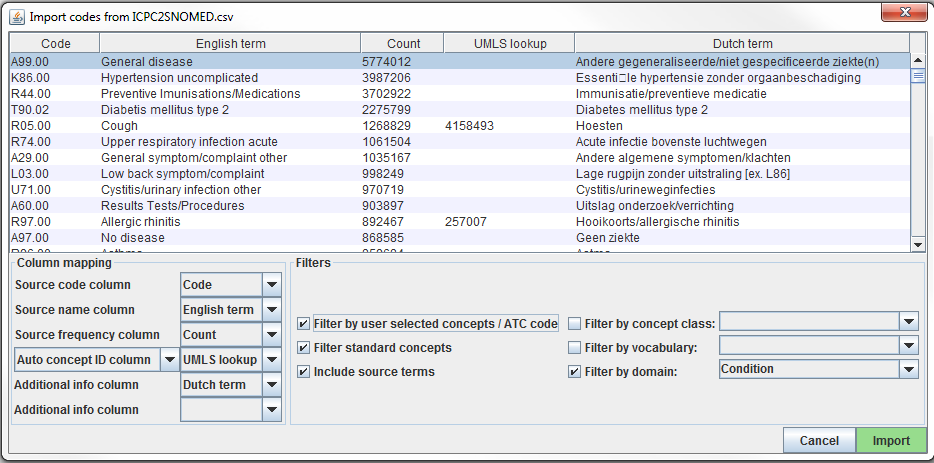
\includegraphics[width=1\linewidth]{images/ExtractTransformLoad/usagiImport} 

}

\caption{Usagiコード入力画面}\label{fig:usagiImport}
\end{figure}

「Column mapping」セクション(左下)では、インポートしたテーブルをUsagiに対してどのように使用するかを定義します。ドロップダウンメニューにマウスを合わせると、それぞれの列の定義が表示されるポップアップが表示されます。Usagiは「Additional info」列をソースコードとボキャブラリコンセプトコードを関連付けるための情報として使用しませんが、この追加情報はソースコードマッピングを確認する際に役立つ場合があるため、含めるべきでしょう。

最後に、「Filters」セクション(右下)では、Usagiがマッピングする際の制限をいくつか設定できます。例えば、図\ref{fig:usagiImport}では、ユーザーはソースコードをコンディションドメインのコンセプトのみにマッピングしています。デフォルトでは、Usagiは標準コンセプトのみにマッピングしますが、「Filter standard concepts」オプションをオフにすると、分類コンセプトも考慮されます。各フィルターについての追加情報は、異なるフィルター上にマウスカーソルを移動させます。

特別なフィルターとして「Filter by automatically selected concepts / ATC code」があります。検索を制限する情報がある場合、CONCEPT\_IDSのリストまたはATCコードをAuto concept ID列で指定された列に記述することで、検索を制限することができます(セミコロンで区切ります)。例えば、医薬品の場合、各医薬品にすでにATCコードが割り当てられている場合があります。ATCコードはRxNormの医薬品コードを一意に識別するものではありませんが、ボキャブラリのATCコードに該当するコンセプトのみに検索対象を限定するのに役立ちます。ATCコードを使用するには、以下の手順に従います。:

\begin{enumerate}
\def\labelenumi{\arabic{enumi}.}
\tightlist
\item
  Column mappingセクションで、``Auto concept ID column''から''ATC column''に切り替えます。
\item
  Column mappingセクションで、ATCコードを含む列を''ATC column''として選択します。
\item
  フィルターセクションで「ユーザーが選択したコンセプト/ATCコードによるフィルター」をオンにします。
\end{enumerate}

ATCコード以外の情報源を使用して制限することもできます。上図の例では、UMLSから派生した部分的なマッピングを使用してUsagiの検索を制限しています。この場合、``Auto concept ID column'' を使用する必要があります。

すべての設定が完了したら、``Import'' ボタンをクリックしてファイルをインポートします。ファイルのインポートには、ソースコードをマッピングするためにボキャブラリの類似性アルゴリズムが実行されるため、数分かかります。

\subsubsection*{ソースコードからボキャブラリへのコンセプトマップの確認}\label{ux30bdux30fcux30b9ux30b3ux30fcux30c9ux304bux3089ux30dcux30adux30e3ux30d6ux30e9ux30eaux3078ux306eux30b3ux30f3ux30bbux30d7ux30c8ux30deux30c3ux30d7ux306eux78baux8a8d}
\addcontentsline{toc}{subsubsection}{ソースコードからボキャブラリへのコンセプトマップの確認}

ソースコードの入力ファイルをインポートすると、マッピング処理が始まります。図 \ref{fig:usagiOverview} では、Usagi の画面は、コンセプトテーブル、選択されているマッピング・セクション、 検索を実行する場所の 3 つの主要な部分で構成されていることがわかります。いずれのテーブルでも、右クリックで表示/非表示の列を選択でき、視覚的な複雑さを軽減できます。

\begin{figure}

{\centering 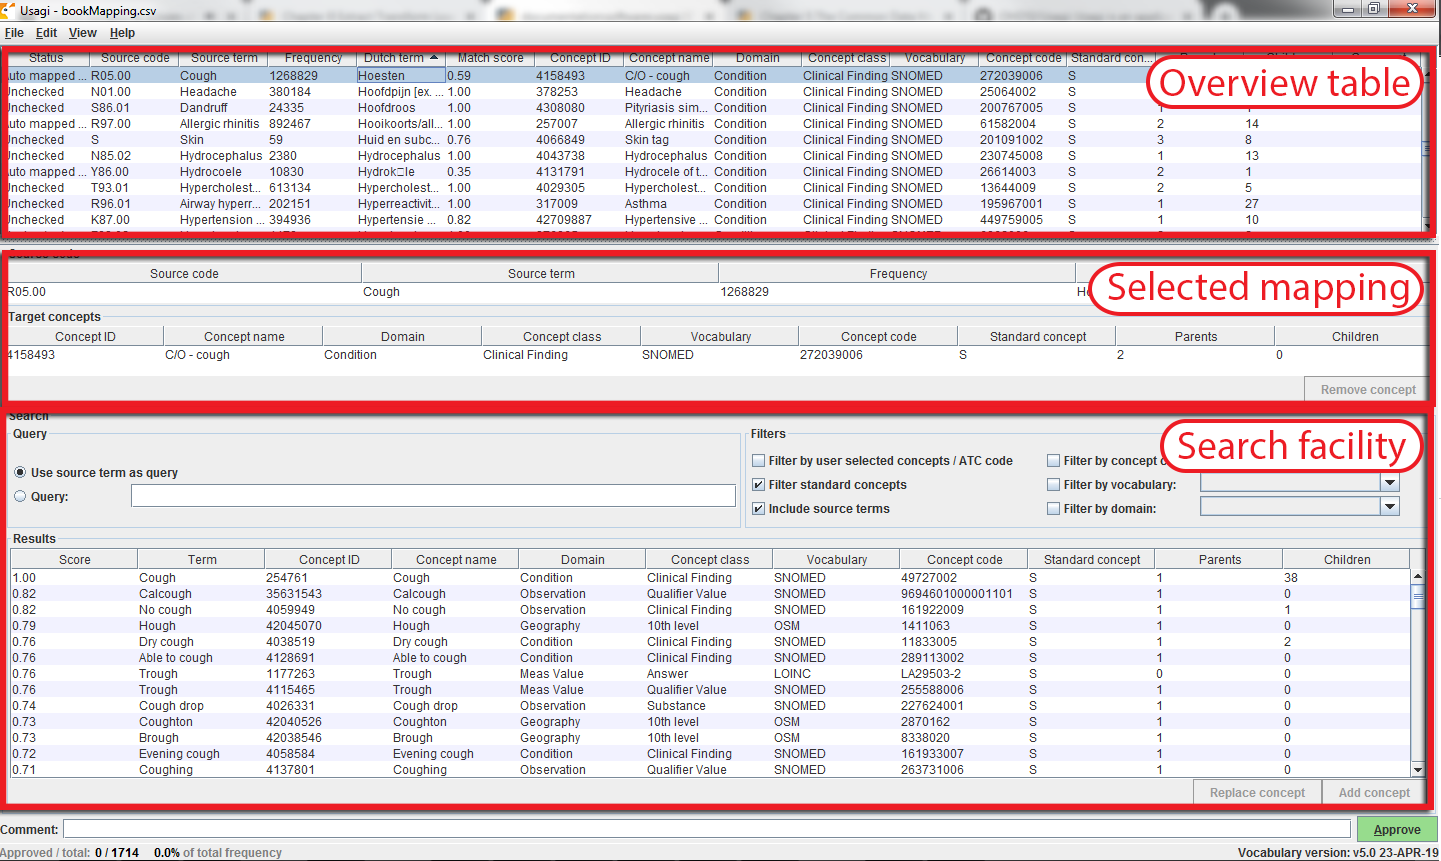
\includegraphics[width=1\linewidth]{images/ExtractTransformLoad/usagiOverview} 

}

\caption{Usagiでのソースコード入力画面}\label{fig:usagiOverview}
\end{figure}

\subsubsection*{提案されたマッピングの承認}\label{ux63d0ux6848ux3055ux308cux305fux30deux30c3ux30d4ux30f3ux30b0ux306eux627fux8a8d}
\addcontentsline{toc}{subsubsection}{提案されたマッピングの承認}

「コンセプトテーブル」には、ソース・コードとコンセプトの現在のマッピングが表示されます。ソース・コードをインポートした直後は、このマッピングには、ボキャブラリの類似性と任意の検索オプションに基づいて自動的に生成されたマッピング候補が含まれます。図 \ref{fig:usagiOverview} の例では、ユーザーがドメインをコンディションに限定しているため、オランダ語のコンディションコードの英語名がコンディションドメインの標準コンセプトにマッピングされています。Usagi は、ソースコードの説明とコンセプト名および同義語を比較して、最適な一致を見つけます。ユーザは ``Include source terms'' (ソース用語を含める) を選択していたため、Usagi は、特定のコンセプトにマッピングされるボキャブラリ内のすべてのソースコンセプトの名前と同義語も考慮しました。Usagi がマッピングできない場合は、CONCEPT\_ID = 0 にマッピングされます。

ソース・コードを関連する標準ボキャブラリにマッピングする際には、コーディング・システムの経験がある人が支援することをお勧めします。その担当者は、``Overview Table'' (概要テーブル) のコードごとに作業して、Usagi が提案したマッピングを受け入れるか、新しいマッピングを選択します。例えば、図 @(ref:fig:usagiOverview) では、オランダ語の ``Hoesten'' は英語の ``Cough'' (咳嗽)に翻訳されています。Usagiは ``Cough'' を使って、``4158493-C/O - cough''というボキャブラリコンセプトにマッピングしました。このマッチしたペアのマッチングスコアは0.58でした(マッチングスコアは通常0~1で、1は確実に一致することを意味します)。一致スコア0.58は、Usagiがオランダ語のコードをSNOMEDにどの程度うまくマッピングできたかについて、あまり確信がないことを意味します。このマッピングで問題ないと思われる場合は、画面右下の緑色の''Approve (承認)'' ボタンを押すことで、このマッピングを承認することができます。

\subsubsection*{新しいマッピングの検索}\label{ux65b0ux3057ux3044ux30deux30c3ux30d4ux30f3ux30b0ux306eux691cux7d22}
\addcontentsline{toc}{subsubsection}{新しいマッピングの検索}

Usagiがマップを提案した場合、ユーザはより良いマッピングを見つけるか、マップをコンセプトなし(CONCEPT\_ID = 0)に設定する必要があります。図 \ref{fig:usagiOverview}の例では、オランダ語の 「Hoesten」を 「Cough」と訳しています。Usagiの提案は、UMLSから自動的に導出されたマッピングで識別されたコンセプトによって制限されており、結果は最適ではないかもしれません。検索機能では、実際のボキャブラリ自体または検索ボックスのクエリを使用して、他のコンセプトを検索することができます。

手動の検索ボックスを使用する場合、Usagiはあいまい検索を使用し、ANDやORのような論理演算子はサポートしていないことに留意する必要があります。

例を続けると、より適切なマッピングを見つけるために「Cough」という検索語を使用したとします。検索機能の「クエリ」セクションの右側には「フィルタ」セクションがあり、検索語を検索する際にボキャブラリから結果を絞り込むオプションがあります。この場合、標準コンセプトのみを検索したいことが分かっているため、標準コンセプトにマッピングされているボキャブラリ内のソースコンセプトの名前と同義語に基づいてコンセプトを検索することも可能です。

これらの検索条件を適用すると、「254761-Cough」が見つかり、これがオランダ語のコードにマッピングする適切なボキャブラリコンセプトであることが分かります。そのため、「Selected Source Code(選択されたソースコード)」 セクションの更新後に表示される 「Replace concept (コンセプトを置換する)」 ボタンを押し、「Approve (承認)」 ボタンを押します。また、「Add concept (コンセプトの追加)」 ボタンもあり、複数の標準化されたボキャブラリのコンセプトを 1 つのソースコードにマッピングすることができます。(例えば、ソースコードによっては、複数の疾患をひとまとめにしている場合がありますが、標準化ボキャブラリではひとまとめにしていない場合があります)。

\subsubsection*{コンセプト情報}\label{ux30b3ux30f3ux30bbux30d7ux30c8ux60c5ux5831}
\addcontentsline{toc}{subsubsection}{コンセプト情報}

マッピングする適切なコンセプトを探す場合、コンセプトの「社会性」を考慮することが重要です。コンセプトの意味は、そのコンセプトの階層における位置に部分的に依存することがあります。また、ボキャブラリの中には、階層関係がほとんどない、あるいは全くない「孤立したコンセプト」が存在することがあり、それらはターゲットにするコンセプトとしては適していません。また、Usagiは概念の親子関係の数を頻繁に報告しますが、ALT + Cキーを押すか、上部メニューバーのview (閲覧)-\textgreater{} Concept information (コンセプト情報) を選択することで、より多くの情報を表示することもできます。

\begin{figure}

{\centering 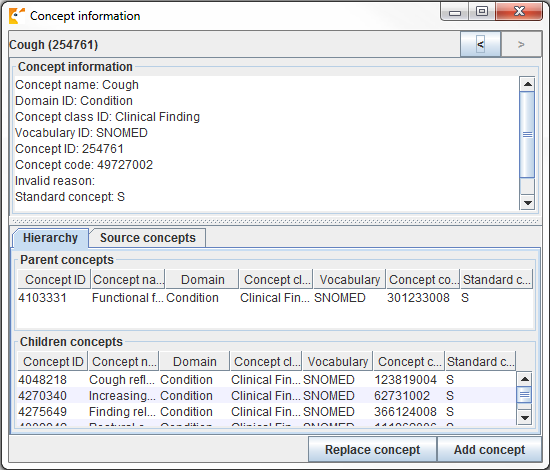
\includegraphics[width=1\linewidth]{images/ExtractTransformLoad/usagiConceptInfo} 

}

\caption{Usagi コンセプト情報パネル}\label{fig:usagiConceptInfo}
\end{figure}

図 \ref{fig:usagiConceptInfo} は、コンセプト情報パネルを示しています。このパネルには、コンセプトに関する一般的な情報、親、子、そのコンセプトにマッピングされるその他のソースコードが表示されます。このパネルを使用して階層を移動し、別のターゲット・コンセプトを選択することができます。

すべてのコードがチェックされるまで、コードごとにこのプロセスを続行します。画面上部のソースコードのリストで、列見出しを選択すると、コードを並べ替えることができます。通常、頻度の高いコードから低いコードに並べ替えることをお勧めします。画面左下には、マッピングが承認されたコードの数と、そのコードの出現回数が表示されます。

マッピングにコメントを追加することもでき、マッピングがどのように決定されたのかを記録するのに役立ちます。

\subsubsection*{ベスト・プラクティス}\label{ux30d9ux30b9ux30c8ux30d7ux30e9ux30afux30c6ux30a3ux30b9}
\addcontentsline{toc}{subsubsection}{ベスト・プラクティス}

\begin{itemize}
\tightlist
\item
  コーディングスキームの経験がある人に参加してもらってください。
\item
  列名をクリックすると、「コンセプトテーブル」の列を並べ替えることができます。``Match Score (マッチングスコア)''で並べ替えると、Usagiが最も信頼するコードを最初に確認でき、かなりの数のコードを迅速に除外できる可能性があります。また、``Frequency (頻度)'' での並べ替えも重要です。頻度に利用されるコードとそうでないコードに重点的に取り組むことが重要です。
\item
  場合によっては、CONCEPT\_ID = 0にマッピングしても問題ありませんが、一部のコードは適切なマッピングが見つからず、また、一部のコードは適切なマッピングがないだけかもしれません。
\item
  コンセプトの文脈、特にその親と子を考慮することが重要です。
\end{itemize}

\subsubsection*{Usagiで作成されたマッピングのエクセウポート}\label{usagiux3067ux4f5cux6210ux3055ux308cux305fux30deux30c3ux30d4ux30f3ux30b0ux306eux30a8ux30afux30bbux30a6ux30ddux30fcux30c8}
\addcontentsline{toc}{subsubsection}{Usagiで作成されたマッピングのエクセウポート}

USAGI 内でマッピングしたら、それをエクスポートしてボキャブラリ SOURCE\_TO\_CONCEPT\_MAP テーブルに追加するのが、次に進むための最良の方法です。

マッピングをエクスポートするには、File (ファイル) -\textgreater{} Export source\_to\_concept\_map (ソースからコンセプトへのマッピングをエクセウポート) を選択します。どのSOURCE\_VOCABULARY\_IDを使用するかを尋ねるポップアップが表示されるので、短いID (識別子) を入力ください。UsagiはこのIDをSOURCE\_VOCABULARY\_IDとして使用し、SOURCE\_TO\_CONCEPT\_MAPテーブルで特定のマッピングを識別できるようにします。

SOURCE\_VOCABULARY\_IDを選択後、出力したCSVに名前を付けて保存します。出力したCSVの構造はSOURCE\_TO\_CONCEPT\_MAPテーブルの構造と同じです。このマッピングは、ボキャブラリのSOURCE\_TO\_CONCEPT\_MAPテーブルに追加できます。また、上記の手順で定義したSOURCE\_VOCABULARY\_IDを定義するVOCABULARYテーブルに単一の行を追加することも意味があります。最後に、「Approved (承認)」ステータスのマッピングのみがCSVファイルにエクスポートされることに留意ください。マッピングをエクスポートするには、USAGIでマッピングを完了する必要があります。

\subsubsection*{Usagiで作成されたマッピングの更新}\label{usagiux3067ux4f5cux6210ux3055ux308cux305fux30deux30c3ux30d4ux30f3ux30b0ux306eux66f4ux65b0}
\addcontentsline{toc}{subsubsection}{Usagiで作成されたマッピングの更新}

多くの場合、マッピングは一度だけの作業ではありません。データが更新されると、新しいソースコードが追加され、ボキャブラリが定期的に更新されるため、マッピングの更新が必要になる場合があります。

ソース・コードのセットが更新された場合は、次の手順で更新できます。

\begin{enumerate}
\def\labelenumi{\arabic{enumi}.}
\tightlist
\item
  新しいソースコードファイルをインポートします。
\item
  File (ファイル) -\textgreater{} Apply previous mapping (以前のマッピングを適用する) を選択します。
\item
  古いマッピングから引き継いだ承認済みのマッピングを継承していないコードを特定し、それらを通常通りマッピングします。
\end{enumerate}

ボキャブラリが更新された場合は、以下の手順に従います:

\begin{enumerate}
\def\labelenumi{\arabic{enumi}.}
\tightlist
\item
  Athena から新しいボキャブラリファイルをダウンロードします。
\item
  Usagi インデックスを再構築します(Help (ヘルプ) -\textgreater{} Rebuild index (インデックスを再構築する))。
\item
  マッピング・ファイルを開きます。
\item
  新しいバージョンのボキャブラリで標準コンセプトでなくなったコンセプトにマッピングされるコードを特定し、より適切なターゲットコンセプトを見つけます。
\end{enumerate}

\section{ステップ 3: ETLの実装}\label{ux30b9ux30c6ux30c3ux30d7-3-etlux306eux5b9fux88c5}

デザインとコードマッピングを完了すると、ETLプロセスをソフトウェアで実装することができます。ETLの設計段階では、ソースデータとCDMに詳しい人が共同で作業することをお勧めしました。同様に、ETLを実装する際には、大量のデータの取り扱い経験があり、ETLの実装経験がある人が作業を行うことが望ましいでしょう。これは、グループ外の人と協力することや、実装するために技術コンサルタントを雇うことを意味するかもしれません。また、これは一度きりの費用ではないことにも留意する必要があります。今後もETLの維持と運用に、少なくともある程度の時間を割くことのできる担当者やチームを確保しておくことが望ましいでしょう(詳細は第 \ref{CDMandETLMaintenance}部 を参照ください)。

実装の具体的な内容は施設ごとに異なり、インフラストラクチャ、データベースの規模、ETLの複雑さ、利用可能な技術専門知識など多くの要因に依存します。そのため、OHDSIコミュニティはETLの最適な実装方法について正式な推奨は行っていません。シンプルなSQLビルダー、SAS、C\#、Java、Kettleを使用するグループもいます。それぞれに長所と短所があり、技術に精通している人がいなければどれも使えません。

ETLの例をいくつか挙げます(複雑さの順に記載):\index{ETL!implementations}

\begin{itemize}
\tightlist
\item
  ETL-Synthea - Syntheaデータベースを変換するために書かれたSQLビルダー

  \begin{itemize}
  \tightlist
  \item
    \url{https://github.com/OHDSI/etl-synthea}
  \end{itemize}
\item
  ETL-CDMBuilder - 複数のデータベースを変換するためにデザインされた.NETアプリケーション

  \begin{itemize}
  \tightlist
  \item
    \url{https://github.com/OHDSI/etl-cdmbuilder}
  \end{itemize}
\item
  ETL-LambdaBuilder - AWS lambda機能を使用するビルダー

  \begin{itemize}
  \tightlist
  \item
    \url{https://github.com/OHDSI/etl-lambdabuilder}
  \end{itemize}
\end{itemize}

複数回の独立した試みの後、ユーザーフレンドリーな''究極の''ETLツールの開発を断念しました。このようなツールはETLの80\%にはうまく機能しますが、残りの20\%については、ソースデータベース固有の低レベルのコードを記述する必要があります。

技術担当者が実装を開始する準備ができたら、ETLデザイン文書を彼らと共有するべきです。ドキュメントには開発を開始するための十分な情報が含まれているはずですが、開発プロセス中に開発者がETL設計者に質問できるようにしておくことが重要です。設計者にとっては明確な論理も、データやCDMに不慣れな実装者にはわかりにくいこともあります。実装フェーズはチーム全体の作業として維持するべきです。すべてのロジックが正しく実行されたという点で両グループが合意するまで、実装者と設計者がそれぞれCDMの作成とテストを行うプロセスを経ることが、適切な方法であると考えられます。

\section{ステップ 4: 品質管理}\label{ux30b9ux30c6ux30c3ux30d7-4-ux54c1ux8ceaux7ba1ux7406}

抽出、変換、読込のプロセスでは品質管理は反復的なプロセスとなります。典型なパターンは、ロジックの記述-\textgreater ロジックの実装-\textgreater ロジックのテスト-\textgreater ロジックの修正・記述です。CDMをテストする方法はいくつもありますが、以下は長年にわたるETL実装を通じてコミュニティ全体で開発された推奨手順です。 \index{ETL!quality control}

\begin{itemize}
\tightlist
\item
  ETL設計文書、コンピュータコード、およびコードマッピングのレビューどんな人でも間違いを犯す可能性があるため、常に少なくとももう1人の人間が、実施された内容を確認すべきです。

  \begin{itemize}
  \tightlist
  \item
    コンピュータコードにおける最大の課題は、ネイティブデータのソースコードが標準コンセプトにどのようにマッピングされるかに起因します。特に日付特有のコード(NDCなど)の場合、マッピングが厄介になることがあります。どの領域でもマッピングが行われる場合は、正しいソースボキャブラリが適切なコンセプトIDに変換されているかを必ず再確認してください。
  \end{itemize}
\item
  ソースデータとターゲットデータのサンプルに関する情報を手動で比較します。

  \begin{itemize}
  \tightlist
  \item
    理想的には、多数のユニークレコードを持つ人物のデータを1件ずつ確認すると役立つでしょう。CDMのデータが合意されたロジックに基づいて期待される形になっていない場合、1人の人物のデータを追跡することで問題が浮き彫りになる可能性があります。
  \end{itemize}
\item
  ソースデータとターゲットデータの全体的なカウントを比較します。

  \begin{itemize}
  \tightlist
  \item
    特定の問題にどのように対処するかによって、カウントに期待される多少の差異が生じるかもしれません。たとえば、一部のコラボレーターは、NULL 性別を持つ人々を削除することを選択しています。なぜなら、そのような人々は分析には含まれないからです。また、CDM における来院は、ネイティブデータにおける来院またはビジットとは異なる方法で構築されている場合もあります。したがって、ソースデータと CDM データの全体的なカウントを比較する際には、これらの相違を考慮し、予想しておくことが重要です。
  \end{itemize}
\item
  ソースデータで既済の研究をCDMバージョンで再現します。

  \begin{itemize}
  \tightlist
  \item
    これはソースデータとCDMバージョンとの間の主な相違点を理解するのに適した方法ですが、多少時間がかかります。
  \end{itemize}
\item
  ETLで対処すべきソースデータのパターンを再現するユニットテストを作成します。例えば、ETLで性別情報が欠落している患者を削除するよう指定されている場合、性別が未設定の人物のユニットテストを作成し、ビルダーがそれをどのように処理するかを評価します。

  \begin{itemize}
  \tightlist
  \item
    ユニットテストは、ETL変換の品質と精度を評価する際に非常に便利です。通常、変換元のデータ構造を模倣したより小規模なデータセットを作成します。このデータセット内の各個人またはレコードは、ETL文書に記載されている特定のロジックをテストする必要があります。この方法を使用すると、問題を簡単に追跡し、エラーが発生したロジックを特定することができます。また、小規模であるため、コンピュータコードを非常に迅速に実行でき、より迅速な反復とエラーの特定が可能になります。
  \end{itemize}
\end{itemize}

以上がETLの観点から品質管理にアプローチするハイレベルの方法です。OHDSIコミュニティ内で進行中のデータ品質への取り組みの詳細については、第 \ref{DataQuality} 章を参照ください。

\section{ETLの規約とTHEMIS}\label{etlux306eux898fux7d04ux3068themis}

データをCDMに変換するグループが増えるにつれ、特定の状況でETLがどのように対処すべきかを明確にする必要があることが明らかになりました。例えば、出生年が欠けている個人レコードの場合、ETLはどうすべきでしょうか?CDMの目標はヘルスケアデータを標準化することですが、各グループが特定のデータシナリオを異なる方法で処理すると、ネットワーク全体でデータを体系的に使用することが難しくなります。

OHDSIコミュニティは、一貫性を向上させるために慣行を文書化し始めました。OHDSIコミュニティが合意したこれらの定義された慣行は、CDM Wikiで参照できます\footnote{\url{https://github.com/OHDSI/CommonDataModel/wiki}}。各CDMテーブルには、ETLを設計する際に参照できる独自の慣行セットがあります。たとえば、出生年の月日が欠けている個人は許容されますが、出生年が欠けている場合、その個人は除外する必要があります。ETLを設計する際には、コミュニティと一貫性のある設計上の決定を行うためにこれらの慣行を参照ください。

すべてのデータシナリオを文書化し、発生した場合に何をするかをドキュメント化することは不可能ですが、一般的なシナリオを文書化しようとしているOHDSIのワークグループがあります。THEMIS\footnote{\url{https://github.com/OHDSI/Themis}}は、コミュニティ内で慣行を収集し、それを明確にし、コミュニティと共有し、最終的な慣行をCDM Wikiに文書化するメンバーで構成されています。THEMISは、古代ギリシャの神々を司る女神で、秩序、公正、法、自然法、慣習を司る存在であり、このグループの任務にふさわしいと考えられました。ETLを実行する際に、どのように処理すべきか判断に迷うシナリオがあった場合、THEMISはそのシナリオについてOHDSIフォーラムに質問を投げかけることを推奨しています\footnote{\url{http://forums.ohdsi.org/}}。質問があるということは、おそらくコミュニティ内の他のメンバーも同じ疑問を抱いている可能性が高いでしょう。THEMISはこれらの議論、ワークグループの会議、対面式のディスカッションなどを利用して、他に文書化する必要がある慣行についても情報を収集します。

\section{CDMおよびETLのメンテナンス}\label{CDMandETLMaintenance}

ETLをデザインし、マッピングを作成し、ETLを実装し、品質管理措置を構築することは多大な労力を要します。残念ながら、この労力はそこで終わりではありません。最初のCDMが構築されると、ETLメンテナンスのサイクルが継続的に行われます。メンテナンスが必要となる一般的な要因は以下の通りです:ソースデータの変更、ETLのバグ、新しいOMOPボキャブラリのリリース、CDM自体の変更や更新などです。これらが発生すると、ETLドキュメント、ETLを実行するソフトウェアプログラミング、テストケースや品質管理などの更新が必要になる場合があります。

医療データソースは常に変化し続けることがよくあります。新しいデータが利用可能になる場合もあります(例:データに新しい列が追加されるなど)。これまで存在しなかった患者のシナリオが突然現れるかもしれません(例:生まれる前に死亡記録がある新生児患者)。データの理解が改善される可能性はあります(例:入院中の子の出産に関する記録の一部が、請求処理の方法により外来患者として記録されている)。すべてのソースデータの変更がETL処理の変更を引き起こすわけではありませんが、最低限、ETL処理を中断する変更には対処する必要があります。

バグが見つかった場合、それに対処する必要があります。ただし、すべてのバグが同じ重要性を持っているわけではないことを念頭に置くことが重要です。例えば、COSTテーブルではcost列が整数に丸められていたとしましょう(例:ソースデータに\$3.82があったのに、CDMで\$4.00になっている)。データを使用して主に患者の薬剤曝露やコンディションの特性評価を行う研究者が多い場合、このようなバグは重要ではなく、将来的に対処すればよいでしょう。しかし、データを使用する主要な研究者に医療経済学者も含まれていた場合、これは直ちに対処する必要がある重大なバグとなります。

OMOPボキャブラリもまた、ソースデータと同様に常に変化しています。実際、ボキャブラリは1ヶ月に何度も更新されることがあります。各CDMは特定のボキャブラリバージョンで実行されており、新しい改善されたボキャブラリで実行すると、標準化ボキャブラリへのソースコードのマッピング方法に変更が生じる可能性があります。多くの場合、ボキャブラリ間の相違は軽微なものであるため、新しいボキャブラリがリリースされるたびに新しいCDMを構築する必要はありません。しかし、年に1~2回は新しいボキャブラリを採用し、CDMを再処理することが推奨されます。ボキャブラリの新バージョンで変更が生じた場合、ETLコード自体を更新する必要が生じることはまれです。

CDMまたはETLのメンテナンスが必要となる最後の要因は、共通データモデル自体が更新される場合です。コミュニティが成長し、新たなデータ要件が見つかった場合、CDMに追加データを保存する必要が生じる可能性があります。これは、以前はCDMに保存されていなかったデータが新しいCDMバージョンに保存される可能性があることを意味します。既存のCDM構造の変更は頻繁ではありませんが、可能性はあります。例えば、CDMが元のDATEフィールドからDATETIMEフィールドを採用したことで、ETL処理にエラーが発生する可能性があります。CDMバージョンは頻繁にはリリースされず、サイトは移行するタイミングを選択できます。

\section{ETLに関する最終的な考察}\label{etlux306bux95a2ux3059ux308bux6700ux7d42ux7684ux306aux8003ux5bdf}

ETLプロセスが異なる理由は数多くありますが、その主な理由のひとつは、私たちがすべてユニークなソースデータを処理しているため、「すべてに適合する」ソリューションを作成するのが難しいという事実です。しかし、長年の経験から、私たちは次のような教訓を得ました。

\begin{itemize}
\tightlist
\item
  80/20のルール。ソースコードを手動でコンセプトセットにマッピングするのにあまり時間をかけないようにしてください。理想的には、データの大部分をカバーするソースコードをマッピングします。 これだけで、まずスタートを切ることができます。残りのコードについては、ユースケースに基づいて、今後対応することができます。
\item
  研究の品質に見合わないデータが失われることを恐れる必要はありません。これらのレコードは、いずれにしても分析を開始する前に破棄されるものです。代わりに、ETLプロセス中にそれらを削除するだけなのです。
\item
  CDMはメンテナンスが必要です。ETLが完了したからといって、二度と触らないということではありません。生データが変更されるかもしれませんし、コードにバグがあるかもしれません。新しいボキャブラリやCDMの更新があるかもしれません。これらの変更に対応するためのリソースを確保し、ETLが常に最新の状態に保たれるようにしましょう。
\item
  OHDSI CDMの開始、データベースの変換、分析ツールの実行のサポートが必要な場合は、実装者フォーラム\footnote{\url{https://forums.ohdsi.org/c/implementers}}をご覧ください。
\end{itemize}

\section{まとめ}\label{ux307eux3068ux3081-4}

\begin{rmdsummary}
\begin{itemize}
\item
  ETLにアプローチするための一般的に合意されたプロセスが存在します

  \begin{itemize}
  \tightlist
  \item
    データ専門家とCDM専門家が協力してETLを設計する
  \item
    医療知識を持つ人がコードマッピングを作成する
  \item
    技術者がETLを実装する
  \item
    すべての関係者が品質管理に関与する
  \end{itemize}
\item
  OHDSIコミュニティはこれらのステップを促進するためにツールを開発しており、これらは自由に利用できます
\item
  参考にできる多くのETL例や合意された慣行があります
\end{itemize}
\end{rmdsummary}

\section{演習}\label{ux6f14ux7fd2-2}

\begin{exercise}
\protect\hypertarget{exr:exerciseEtl1}{}\label{exr:exerciseEtl1}

ETLプロセスのステップを正しい順序に並べてください:

\begin{enumerate}
\def\labelenumi{\Alph{enumi})}
\tightlist
\item
  データ専門家とCDM専門家が協力してETLを設計する
\item
  技術者がETLを実装する
\item
  医療知識を持つ人がコードマッピングを作成する
\item
  すべての関係者が品質管理に関与する
\end{enumerate}

\end{exercise}

\begin{exercise}
\protect\hypertarget{exr:exerciseEtl2}{}\label{exr:exerciseEtl2}

選択したOHDSIリソースを使用して、表 \ref{tab:exercisePersonTable} に示すPERSONレコードに関する4つの問題点を指摘してください(表はスペースのため省略されています):

\begin{longtable}[]{@{}ll@{}}
\caption{\label{tab:exercisePersonTable} PERSONテーブル}\tabularnewline
\toprule\noalign{}
列 & 値 \\
\midrule\noalign{}
\endfirsthead
\toprule\noalign{}
列 & 値 \\
\midrule\noalign{}
\endhead
\bottomrule\noalign{}
\endlastfoot
PERSON\_ID & A123B456 \\
GENDER\_CONCEPT\_ID & 8532 \\
YEAR\_OF\_BIRTH & NULL \\
MONTH\_OF\_BIRTH & NULL \\
DAY\_OF\_BIRTH & NULL \\
RACE\_CONCEPT\_ID & 0 \\
ETHNICITY\_CONCEPT\_ID & 8527 \\
PERSON\_SOURCE\_VALUE & A123B456 \\
GENDER\_SOURCE\_VALUE & F \\
RACE\_SOURCE\_VALUE & WHITE \\
ETHNICITY\_SOURCE\_VALUE & 提供されていない \\
\end{longtable}

\end{exercise}

\begin{exercise}
\protect\hypertarget{exr:exerciseEtl3}{}\label{exr:exerciseEtl3}VISIT\_OCCURRENCEレコードを生成してみましょう。以下はSyntheaのために書かれたロジック例です:
PATIENT、START、ENDのデータを昇順で並べ替えます。その後、PERSON\_IDごとに、前の行のENDと次の行のSTARTの間に1日以内の時間がある場合、請求の行を統合します。統合された入院患者の請求は1つの入院患者のビジットと見なされ、設定されます:

\begin{itemize}
\tightlist
\item
  MIN(START)をVISIT\_START\_DATEとして設定
\item
  MAX(END)をVISIT\_END\_DATEとして設定
\item
  ``IP''をPLACE\_OF\_SERVICE\_SOURCE\_VALUEとして設定
\end{itemize}

ソースデータに図 \ref{fig:exerciseSourceData} に示されるようなビジットセットがある場合、CDMで生成されるVISIT\_OCCURRENCEレコードはどのようになると予想しますか?
\end{exercise}

\begin{figure}

{\centering 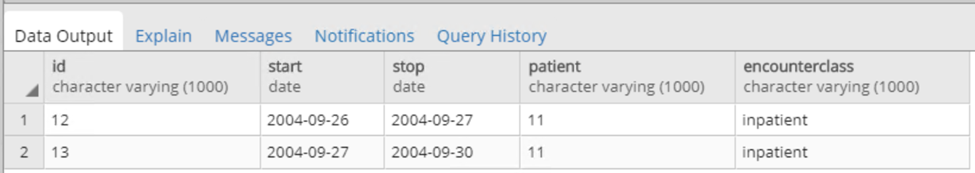
\includegraphics[width=1\linewidth]{images/ExtractTransformLoad/exerciseSourceData} 

}

\caption{例のソースデータ。}\label{fig:exerciseSourceData}
\end{figure}

提案された回答は付録 \ref{Etlanswers} を参照ください。

\part{--翻訳作業中-- データ解析}\label{part-ux7ffbux8a33ux4f5cux696dux4e2d-ux30c7ux30fcux30bfux89e3ux6790}

\chapter{データ解析の使用例}\label{DataAnalyticsUseCases}

\emph{章の著者: David Madigan}

OHDSI 共同研究は、通常、請求データベースや電子カルテデータベースなどの形式で、実世界のヘルスケアデータから信頼性の高いエビデンスを生成することに重点を置いています。OHDSI が重点的に取り組むユースケースは、主に以下の3つのカテゴリーに分類されます。

\begin{itemize}
\tightlist
\item
  特性評価
\item
  集団レベルの推定
\item
  患者レベルの予測
\end{itemize}

以下でこれらについて詳しく説明します。すべてのユースケースにおいて、生成されるエビデンスはデータの限界を継承します; これらの限界については、エビデンスの質に関する本の(第 \ref{EvidenceQuality} 章- 第\ref{MethodValidity}章)で詳しく説明しています。

\section{特性評価}\label{ux7279ux6027ux8a55ux4fa1}

\index{characterization}

特性評価は次のような質問に答えようとします

\begin{quote}
かれらに何が起こったのか?
\end{quote}

データを用いて、コホートやデータベース全体の集団の特性、医療行為、経時的な変化に関する問いに答えることができます。

データが答えを提供できる問いには次のような例があります:

\begin{itemize}
\tightlist
\item
  新たに心房細動と診断された患者のうち、何人がワルファリンの処方を受けたのか?
\item
  人口股関節置換術を受けた患者の平均年齢は?
\item
  65歳以上の患者の肺炎の発生率は?
\end{itemize}

典型的な特性評価は以下のように定式化されます:

\begin{itemize}
\tightlist
\item
  何人の患者が\ldots?
\item
  どのくらいの頻度で\ldots?
\item
  患者の何パーセントが\ldots?
\item
  検査値の分布はどのようになっているか\ldots?
\item
  の患者のHbA1c値は\ldots?
\item
  の患者の検査値は\ldots?
\item
  の患者の曝露期間の中央値は\ldots?
\item
  経時的な傾向は?
\item
  これらの患者が使用している他の薬剤は何か?
\item
  併用療法は?
\item
  の症例が十分にあるか?
\item
  Xを研究は可能か?
\item
  の人口統計は?
\item
  のリスク要因は?(特定のリスク要因を識別する場合、予測ではなく推定)
\item
  の予測因子は?
\end{itemize}

そして期待されるアプトプットは以下の通りです:

\begin{itemize}
\tightlist
\item
  カウントまたはパーセンテージ
\item
  平均
\item
  記述統計
\item
  発生率
\item
  有病率
\item
  コホート
\item
  ルールベースの表現型
\item
  薬剤利用
\item
  疾患の自然経過
\item
  服薬アドヒアランス
\item
  併存疾患のプロファイル
\item
  治療経路
\item
  治療方針
\end{itemize}

\section{集団レベルの推定}\label{ux96c6ux56e3ux30ecux30d9ux30ebux306eux63a8ux5b9a}

\index{population-level estimation}

限定的ではありますが、、データは医療介入の効果に関する因果推論を裏付けることができ、次の問いに答えます

\begin{quote}
因果効果とは何か?
\end{quote}

私たちは因果効果を理解することで、行動の結果を理解したいと考えています。例えば、ある治療法を受けると決めた場合、将来にわたって私たちの身に何が起こるのかがどう変わるのでしょうか?

データは、次のような問いに対する答えを提供することができます:

\begin{itemize}
\tightlist
\item
  新たに心房細動と診断された患者において、治療開始後最初の1年間に、ワルファリンはダビガトランよりも重大な出血を引き起こすか?
\item
  メトホルミンの下痢に対する因果効果は年齢によって異なるか?
\end{itemize}

典型的な集団レベルの効果推定の問いは次のように定式化されます:

\begin{itemize}
\tightlist
\item
  \ldots の効果は?
\item
  介入を行った場合、どうなるのか?
\item
  どちらの治療がより効果的か?
\item
  Yに対するXのリスクは?
\item
  のイベント発生までの時間は?
\end{itemize}

そして、期待されるアウトプットは以下の通りです:

\begin{itemize}
\tightlist
\item
  相対リスク
\item
  ハザード比
\item
  オッズ比
\item
  平均治療効果
\item
  因果効果
\item
  関連
\item
  相関
\item
  安全性監視
\item
  効果の比較
\end{itemize}

\section{患者レベルの予測}\label{ux60a3ux8005ux30ecux30d9ux30ebux306eux4e88ux6e2c}

\index{patient-level prediction}

データベースに収集された患者の医療履歴に基づいて、将来の健康イベントに関する患者レベルの予測を行い、次の問にい答えます

\begin{quote}
私には何が起こるのか?
\end{quote}

データは、以下のような質問に対する答えを提供することができます:

\begin{itemize}
\tightlist
\item
  新たに重度うつ病と診断された特定の患者について、診断後1年以内に自殺を図る確率はどの程度か?
\item
  新たに心房細動と診断され、ワルファリンによる治療開始後1年以内に虚血性脳卒中を発症する確率どの程度か?
\end{itemize}

典型的な患者レベルの予測に関する問いは次のように定式化されます:

\begin{itemize}
\tightlist
\item
  この患者が\ldots になる可能性はどの程度か?
\item
  誰が\ldots の候補となるのか?
\end{itemize}

そして、期待されるアウトプットは以下の通りです:

\begin{itemize}
\tightlist
\item
  個人の確率
\item
  予測モデル
\item
  高リスク/低リスクグループ
\item
  確率的な表現型
\end{itemize}

集団レベルの推定と患者レベルの予測はある程度重複することがあります。例えば、予測の重要なユースケースとしては、特定の患者に薬剤Aが処方された場合の治療結果を予測し、また薬剤Bが処方された場合の同じ治療結果を予測することが挙げられます。現実には、これらの薬剤のうちの1つだけが処方された(例えば薬剤A)と仮定すると、薬剤Aによる治療の結果が実際に起こるかどうかを確認することができます。薬剤Bは処方されていないため、薬剤Bによる治療の結果は予測可能ですが、「反事実」であり、実際には観察されません。予測作業はそれぞれ患者レベルの予測に該当します。しかし、2つの結果の差(または比率)は単位レベルの因果効果であり、代わりに因果効果推定法を用いて推定すべきです。

\begin{rmdimportant}
人々は予測モデルを因果モデルとして誤って解釈する傾向があります。しかし、予測モデルは相関関係のみを示すことができ、因果関係を示すことはできません。例えば、糖尿病は心筋梗塞(MI)の強いリスク要因であるため、糖尿病治療薬の使用は心筋梗塞の強い予測因子であるかもしれません。しかし、糖尿病治療薬の使用を中止すれば心筋梗塞を予防できるというわけではありません!
\end{rmdimportant}

\section{高血圧症におけるユースケース}\label{ux9ad8ux8840ux5727ux75c7ux306bux304aux3051ux308bux30e6ux30fcux30b9ux30b1ux30fcux30b9}

あなたは、高血圧症の第一選択治療として急性心筋梗塞や血管性浮腫果に対するACE阻害薬単独療法とサイアザイド系利尿薬単剤療法の効果を研究することに関心のある研究者です。OHDSIの文献に基づいて、集団レベルの効果推定値を求める問いをすることになると理解していますが、まず、この特定の治療に関する特性評価を行うため、準備をする必要があります。

\subsection{特性評価に関する問い}\label{ux7279ux6027ux8a55ux4fa1ux306bux95a2ux3059ux308bux554fux3044}

急性心筋梗塞は高血圧症患者に起こりうる心血管系の合併症であり、高血圧症に対する有効な治療によってリスクを軽減できるはずです。血管性浮腫は稀ですが重篤になる可能性のあるACE阻害薬の既知の副作用です。あなたは、対象とする曝露(ACE阻害薬の新規使用者およびサイアザイド系利尿薬の新規使用者)のコホートを作成することから始めます(第 \ref{Cohorts}章を参照)。曝露集団のベースライン特性(人口統計学的特性、併存疾患、併用薬など)を要約するため、特性評価(第 \ref{Characterization}章を参照)の解析を実行します。この曝露集団における特定のアウトカムの発生率を推定するために、別の特性評価を実行します。ここでは、「ACE阻害薬およびサイアザイド系利尿薬に曝露された期間に1)急性心筋梗塞および2)血管性浮腫がどのくらいの頻度で発生するか?」という問いをします。これらの特性評価により、集団レベルの効果推定研究を実施できるかどうかの実行可能性を評価し、2つの治療グループが比較可能かどうかを評価し、患者がどちらの治療を選択したかを予測する`リスク因子'を特定することができます。

\subsection{集団レベルの推定問題}\label{ux96c6ux56e3ux30ecux30d9ux30ebux306eux63a8ux5b9aux554fux984c}

集団レベルの効果推定研究(第 \ref{PopulationLevelEstimation}章を参照)は、急性心筋梗塞と血管性浮腫のアウトカムに対するACE阻害薬対サイアザイドの使用の相対リスクを推定します。ここでは、研究診断とネガティブコントロールにより、平均治療効果の信頼性の高い推定値を生成できるかどうかをさらに評価します。

\subsection{患者レベルの予測問題}\label{ux60a3ux8005ux30ecux30d9ux30ebux306eux4e88ux6e2cux554fux984c}

曝露の因果効果とは独立して、アウトカムのリスクが最も高い患者を特定しようとすることにも興味があります。これは患者レベルの予測問題です(第 \ref{PatientLevelPrediction}章を参照)。ここでは、ACE阻害薬の新規ユーザーの中で、治療開始後1年以内に急性心筋梗塞を発症するリスクが最も高い患者を評価する予測モデルを開発します。このモデルにより、ACE阻害薬を初めて処方された患者について、その病歴から観察されたイベントに基づき、今後1年間に急性心筋梗塞を発症する確率を予測することができます。

\section{観察研究の限界}\label{ux89b3ux5bdfux7814ux7a76ux306eux9650ux754c}

\index{観察研究の限界}

OHDSIデータベースでは答えを出せない重要な医療問題は数多くあります。以下はその例です。:

\begin{itemize}
\tightlist
\item
  プラセボと比較した介入の因果効果。治療と非治療の比較は可能であっても、プラセボ治療との比較による因果効果を考慮することはできない場合があります。
\item
  市販薬に関するもの。
\item
  多くのアウトカムやその他の変数は、ほとんど記録されていないか、まばらにしか記録されていません。これには、死亡率、行動アウトカム、ライフスタイル、社会経済的地位が含まれます。
\item
  患者は体調が悪いときにしか医療システムを利用しない傾向があるため、治療の有益性を測定することが困難です。
\end{itemize}

\subsection{誤ったデータ}\label{ux8aa4ux3063ux305fux30c7ux30fcux30bf}

OHDSIデータベースに記録された臨床データは、臨床の現実と乖離している可能性があります。例えば、患者が心筋梗塞を経験していないにもかかわらず、患者記録に心筋梗塞のコードが含まれている可能性があります。同様に、検査値が誤っていたり、処置の誤ったコードがデータベースに表示されている可能性もあります。第 \ref{DataQuality} 章や第 \ref{ClinicalValidity} 章では、これらの問題について説明しており、ベストプラクティスでは、このような問題を可能な限り特定し、修正することを目指しています。ただし、誤ったデータは必然的にある程度は残存し、その後の分析の妥当性を損なう可能性はあります。広範な文献が、データエラーを考慮した統計的推論の調整に焦点を当てており、例えば、Fuller \citet{fuller2009measurement} を参照ください。

\subsection{欠損データ}\label{ux6b20ux640dux30c7ux30fcux30bf}

\index{欠損データ}

OHDSIデータベースにおける欠損は微妙な課題を呈します。データベースに記録されるべき健康イベント(例:処方、検査値など)が記録されていない場合、それは「欠損」となります。統計学の文献では、「完全にランダムに欠損」、「ランダムに欠損」、「非ランダムに欠損」など欠損のタイプを区別し、複雑性を増す手法によってこれらのタイプに対処しようとしています。\citet{perkins2017principled} はこのトピックに関する有用な入門書を提供しています。

\section{まとめ}\label{ux307eux3068ux3081-5}

\begin{rmdsummary}
\begin{itemize}
\item
  観察研究では、3つの大きなユースケースのカテゴリーを区別します。
\item
  \textbf{特性評価}は「彼らに何が起こったか?」という問いに答えようとします。
\item
  \textbf{集団レベルの推定}は「因果効果は何か?」という問いに答えようとします。
\item
  \textbf{患者レベルの予測}は「私には何が起こるのか?」という問いに答えようとします。
\item
  予測モデルは因果モデルではありません。強い予測因子に介入してもアウトカムに影響を与えると考える理由はありません。
\item
  観察医療データでは答えられない問いもあります。
\end{itemize}
\end{rmdsummary}

\section{演習}\label{ux6f14ux7fd2-3}

\begin{exercise}
\protect\hypertarget{exr:exerciseUseCases1}{}\label{exr:exerciseUseCases1}

これらの質問はどのユースケースのカテゴリーに属しますか?

\begin{enumerate}
\def\labelenumi{\arabic{enumi}.}
\item
  最近非ステロイド性抗炎症薬(NSAID)を投与された患者における消化管(GI)出血の発生率を計算する。
\item
  ベースラインの特性に基づいて、特定の患者が今後1年間にGI出血を経験する確率を計算する。
\item
  セレコキシブと比較してジクロフェナクによるGI出血のリスク増加を推定する。
\end{enumerate}

\end{exercise}

\begin{exercise}
\protect\hypertarget{exr:exerciseUseCases2}{}\label{exr:exerciseUseCases2}ジクロフェナクによるGI出血のリスクがプラセボ(偽薬)に比べてどの程度高まるかを推定したい。医療観察データを使用して、この推定を行うことは可能だろうか?
\end{exercise}

推奨される解答は、付録 \ref{UseCasesanswers}を参照ください。

\chapter{--翻訳作業中-- OHDSI 分析ツール}\label{OhdsiAnalyticsTools}

\emph{章の著者: Martijn Schuemie \& Frank DeFalco}

OHDSIは、患者レベルの観察データに対するさまざまなデータ分析のユースケースをサポートするための幅広いオープンソースツールを提供しています。これらのツールの共通点は、すべて共通データモデル(CDM)を使用して1つ以上のデータベースと相互にやりとりできることです。さらに、これらのツールはさまざまなユースケースに対して分析を標準化します。ゼロから始める必要はなく、標準テンプレートに入力することで分析を実装できます。これにより、分析が容易になり、再現性と透明性が向上します。例として、発生率を計算する方法は無数にあるように思われますが、OHDSIツールではいくつかの選択肢で指定でき、同じ選択肢を選んだ人は同じ方法で発生率を計算します。

本章では、最初に分析を実装するさまざまな方法を説明し、分析で採用できる戦略について説明します。次に、さまざまなOHDSIツールとそれらがどのようにさまざまなユースケースにどのように適合するかを検討します。

\section{分析の実装}\label{analysisImplementation}

図 \ref{fig:implementations} は、CDMを使用してデータベースに対して研究を実装するために選択できるさまざまな方法を示しています。 \index{analysis implementation}

\begin{figure}

{\centering 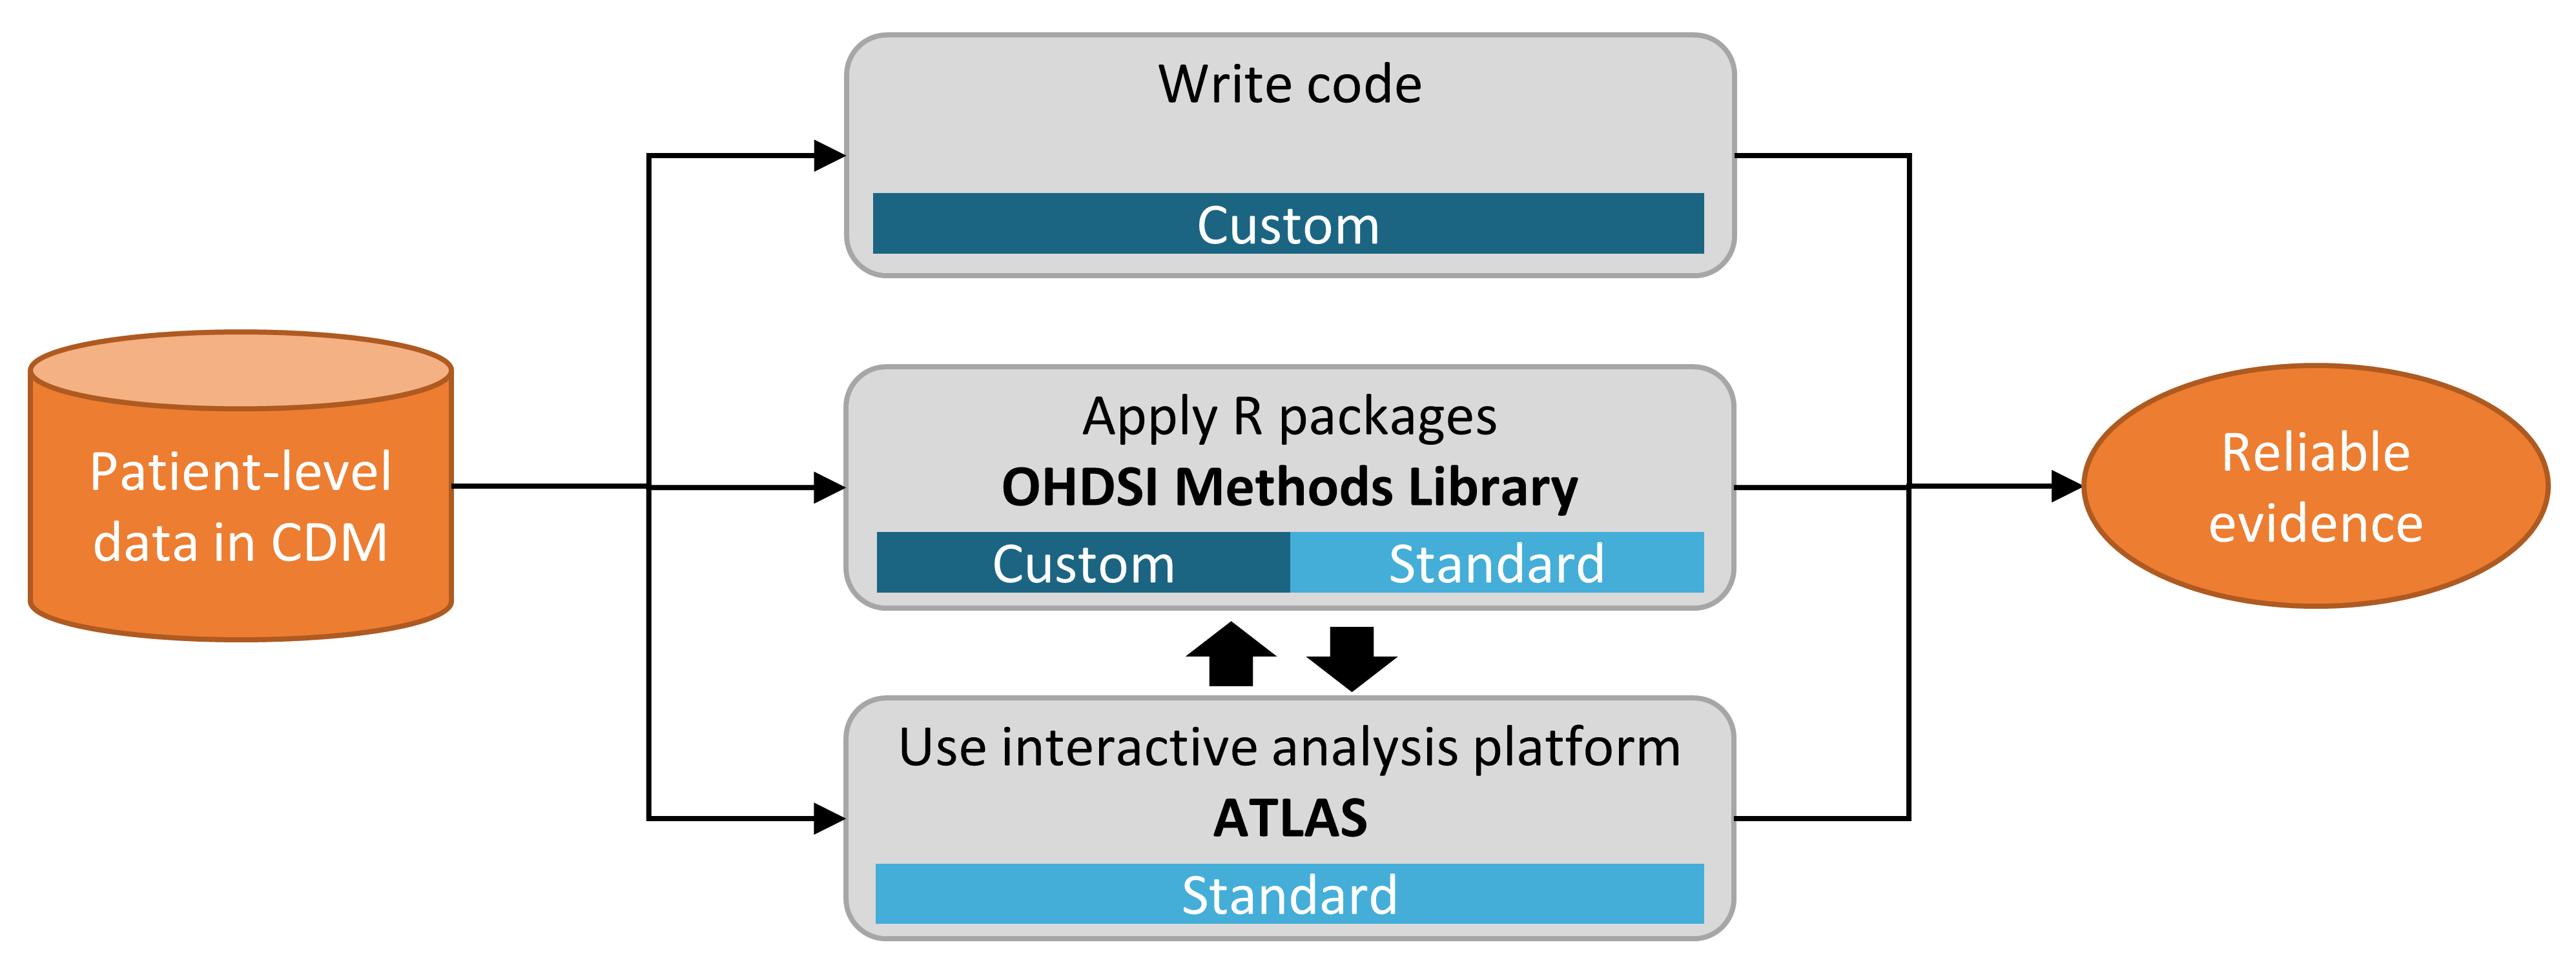
\includegraphics[width=0.9\linewidth]{images/OhdsiAnalyticsTools/implementations} 

}

\caption{CDMのデータに対する分析を実装するさまざまな方法}\label{fig:implementations}
\end{figure}

研究を実装するための主なアプローチは3つあります。最初の方法は、OHDSIが提供するツールを一切使用しないカスタムコードを作成することです。R、SAS、またはその他の言語で新規の分析を作成することができます。これにより最大の柔軟性が得られ、特定の分析がツールでサポートされていない場合は唯一の選択肢となるかもしれません。しかし、この方法は高度な技術、時間、労力を必要とし、分析が複雑になるほどコードのエラーを避けることが難しくなります。

2番目の方法は、Rで分析を開発し、\href{https://ohdsi.github.io/MethodsLibrary/}{OHDSI Methods Library}のパッケージを利用する方法です。少なくとも、\href{https://ohdsi.github.io/SqlRender/}{SqlRender}と\href{https://ohdsi.github.io/DatabaseConnector/}{DatabaseConnector}のパッケージを使用できます。これらのパッケージについては、第 \ref{SqlAndR} 章で詳しく説明していますが、PostgreSQL、SQL Server、Oracleなどのさまざまなデータベースプラットフォーム上で同じコードを実行することができます。また、\href{https://ohdsi.github.io/CohortMethod/}{CohortMethod}や\href{https://ohdsi.github.io/PatientLevelPrediction/}{PatientLevelPrediction}などのパッケージでは、CDMに対する高度な分析のためのR関数が提供されており、コードから呼び出すことができます。これには依然として高度な専門知識が必要ですが、検証済のMethods Libraryのコンポーネントを再利用することで、完全にカスタムコードを使用する場合よりも効率的に作業を進めることができ、エラーが発生する可能性も低くなります。

3番目の方法は、プログラマーでなくても幅広く分析を効率的に実行できるウェブベースのツール、\href{https://github.com/OHDSI/Atlas/wiki}{ATLAS}を使用することです。ATLASはMethods Librariesを使用しますが、分析をデザインするための単純なグラフィカルインターフェイスを提供し、多くの場合、分析を実行するために必要なRコードを生成します。ただし、Methods Libraryで利用可能なすべてのオプションをサポートしているわけではありません。大半の研究はATLASを通じて行うことができると予想されますが、2番目の方法が提供する柔軟性を必要とする研究もあります。

ATLASとMethods Libraryは独立したものではありません。ATLASで呼び出される複雑な分析の一部は、Methods Libraryのパッケージへの呼び出しを通じて実行されます。同様に、Methods Libraryで使用されるコホートは、多くの場合、ATLASでデザインされています。

\section{分析戦略}\label{ux5206ux6790ux6226ux7565}

CDMに対する分析を実装するための戦略に加え、例えばカスタムコーディングやMethods Libraryで提供される標準分析コードの利用など、エビデンスを生成するための分析技術を使用する複数の戦略もあります。図 \ref{fig:strategies} は、OHDSIで採用されている3つの戦略を示しています。

\begin{figure}

{\centering 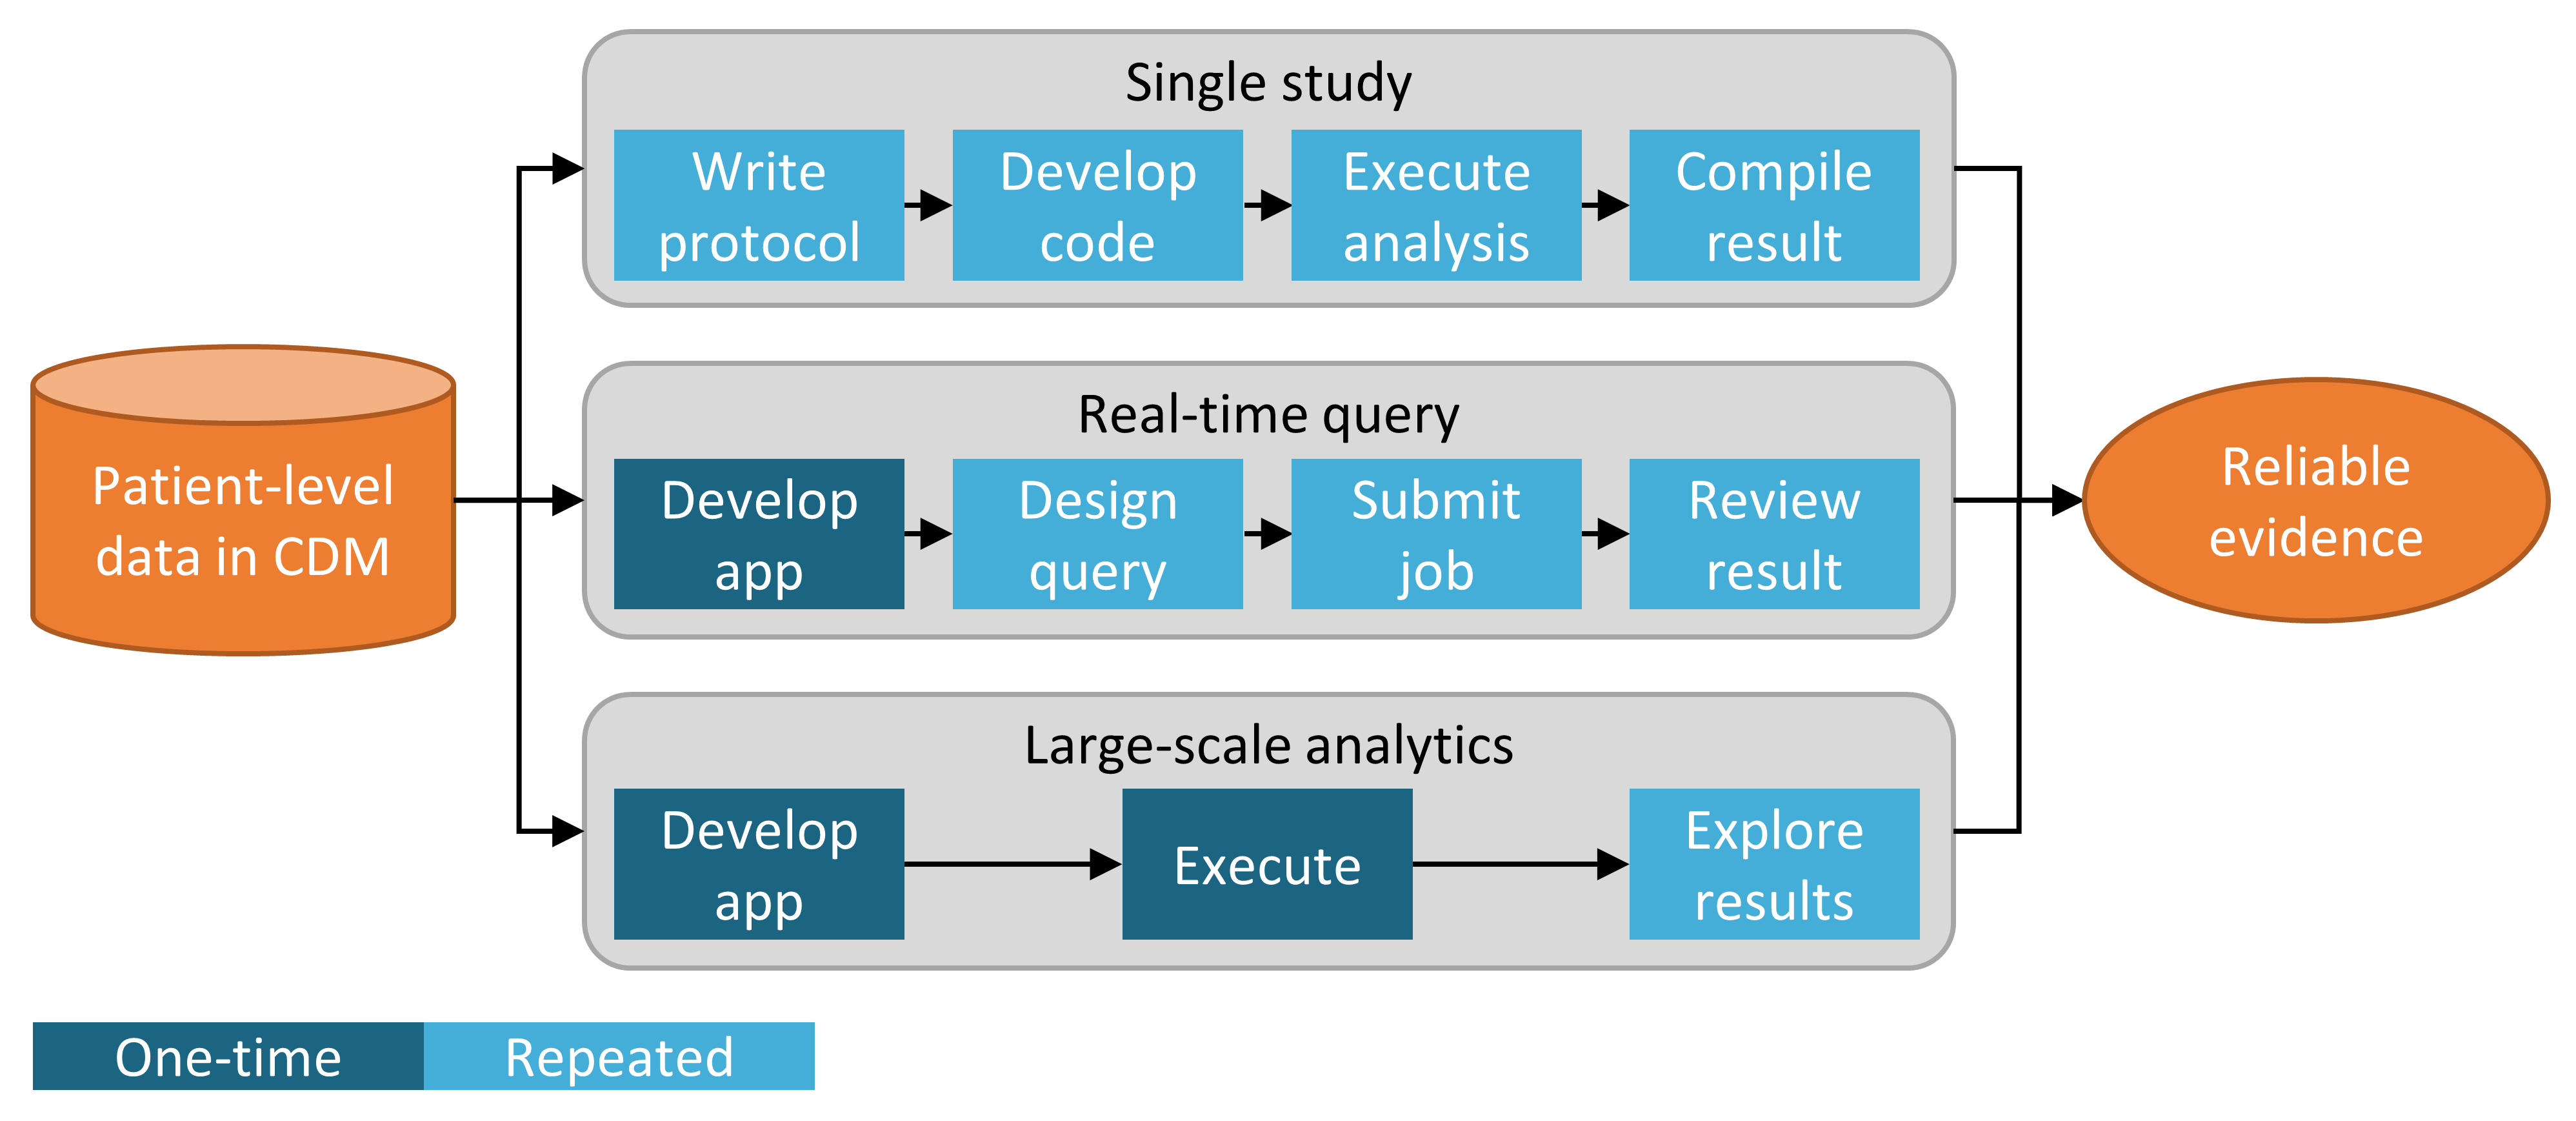
\includegraphics[width=0.9\linewidth]{images/OhdsiAnalyticsTools/strategies} 

}

\caption{(臨床の)問いに対するエビデンスを生成するための戦略}\label{fig:strategies}
\end{figure}

最初の戦略では、各分析を個別の研究として扱います。分析はプロトコルで事前に規定し、コードとして実装し、データに対して実行し、その後、結果をまとめ解釈します。各質問ごとに、すべてのステップを繰り返す必要があります。このような分析の一例は、levetiracetamとphenytoinを比較した際の血管性浮腫のリスクに関するOHDSI研究です\citep{duke_2017}。 ここでは、まずプロトコルが作成され、OHDSI Methods Libraryを使用した分析コードが開発され、OHDSIネットワーク全体で実行され、結果がまとめられて学術誌に公表されました。

第二の戦略では、リアルタイムまたはほぼリアルタイムで特定のクラスの問いに答えられるアプリケーションを開発します。アプリケーションが開発されると、ユーザーはクエリをインタラクティブに定義し、それを送信して結果を表示できます。この戦略の一例は、ATLASのコホート定義および生成ツールです。このツールは、ユーザーが複雑さの異なるコホート定義を指定し、データベースに対してその定義を実行して、さまざまな包含基準と除外基準を満たす人数を確認することができます。

第三の戦略では、同様に問いに焦点を当てますが、その問いのクラス内のすべてのエビデンスを網羅的に生成しようとします。ユーザーは、さまざまなインターフェースを通じて必要に応じてエビデンスを探索できます。一例は、うつ病治療の効果に関するOHDSI研究です\citep{schuemie_2018b}。 この研究では、すべてのうつ病治療が、4つの大規模な観察研究データベースで関心のあるアウトカムの大規模なセットに対して比較されました。17,718の実証的にキャリブレーションされたハザード比と広範な研究診断を含む結果の全セットは、インタラクティブなウェブアプリ \footnote{\url{http://data.ohdsi.org/SystematicEvidence/}} で利用できます。

\section{ATLAS}\label{atlas}

ATLAS は、OHDSI コミュニティが開発した、標準化された患者レベルの観察データを CDM 形式で分析する設計と実行を支援する、無料で公開されているウェブベースのツールです。ATLAS は、OHDSI WebAPI と組み合わせてウェブアプリケーションとして展開され、通常は Apache Tomcat 上でホストされます。リアルタイム分析を行うには、CDM 内の患者レベルデータへのアクセスが必要であるため、通常は組織のファイアウォールのバックにインストールされます。ただし、パブリックなATLAS\textsuperscript{\href{https://ohdsi.github.io/TheBookOfOhdsi/OhdsiAnalyticsTools.html\#fn40}{40}}も存在し、このATLASインスタンスは少数の小規模なシミュレーションデータセットにしかアクセスできませんが、テストやトレーニングなど、多くの目的に使用できます。パブリックなATLASインスタンスを使用して効果の推定や予測研究を完全に定義し、研究を実行するためのRコードを自動的に生成することも可能です。そのコードは、ATLASとWebAPIをインストールすることなく、利用可能なCDMがインストールされている環境であればどこでも実行できます。\index{ATLAS}

\begin{figure}

{\centering 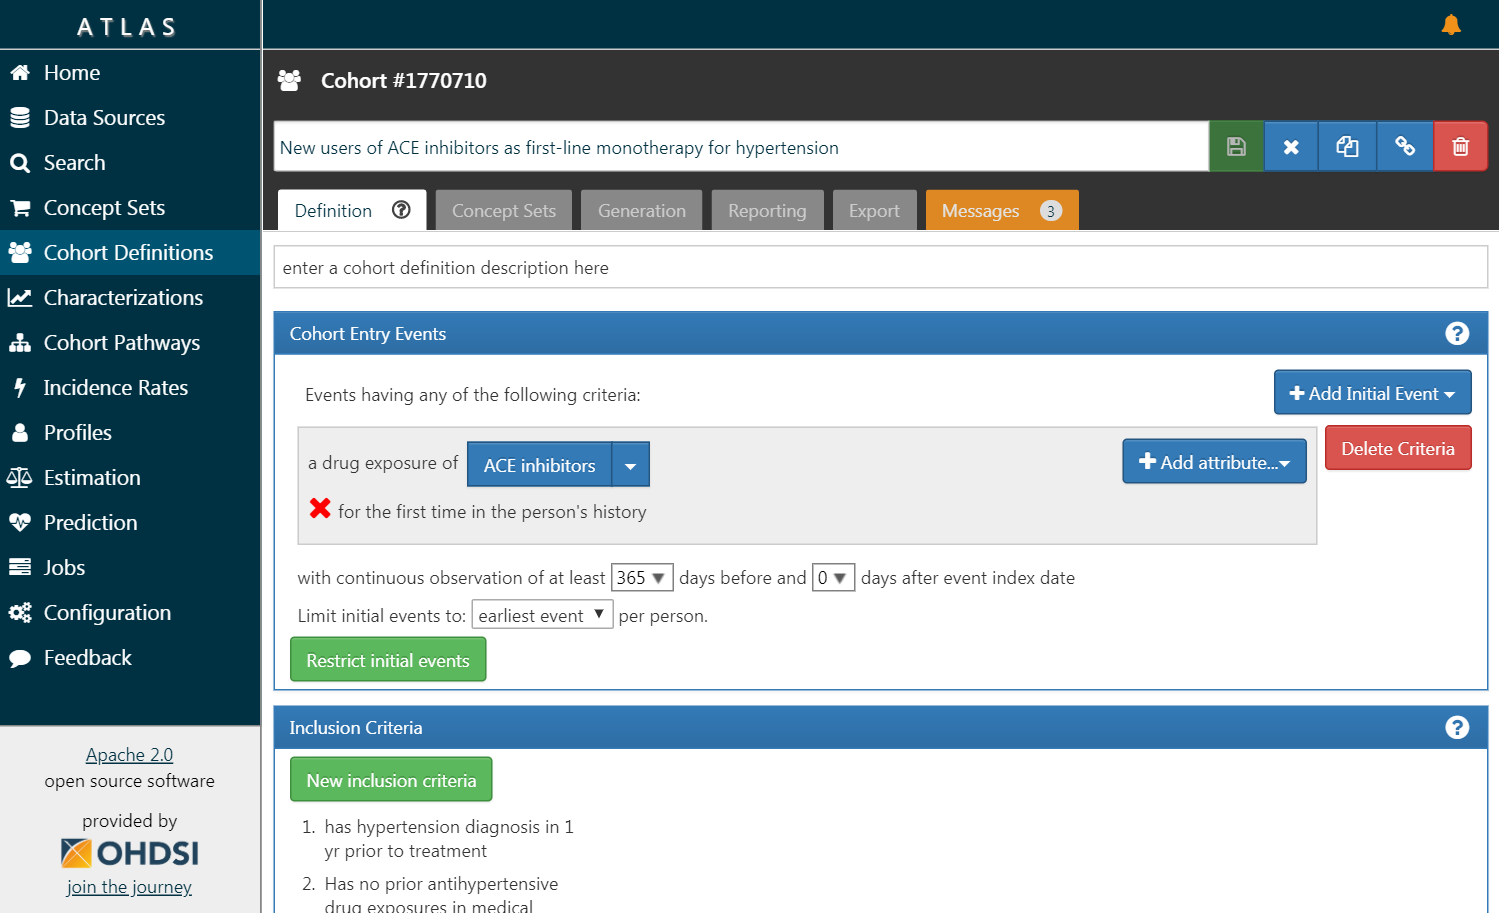
\includegraphics[width=1\linewidth]{images/OhdsiAnalyticsTools/atlas} 

}

\caption{ATLASユーザインタフェース}\label{fig:atlas}
\end{figure}

図 \ref{fig:atlas} にATLASのスクリーンショットを示します。左側にはATLASの様々な機能を示すナビゲーションバーがあります。

\begin{description}
\item[データソース \index{ATLAS!データソース} \index{Achilles|see {ATLAS!データソース}}]
データソースは、ATLASプラットフォームに構成された各データソースの記述的で標準化されたレポートをレビューする機能を提供します。この機能は大規模分析戦略を用いており、、すべての記述は事前に計算されています。データソースについては、第\ref{Characterization}章で説明します。
\item[ボキャブラリ検索 \index{ATLAS!ボキャブラリ検索}]
ATLASはOMOP標準化ボキャブラリを検索し、これらのボキャブラリにどのようなコンセプトが存在するのか、そしてそのコンセプトをどう適用するかを理解するための機能を提供します。この機能については、第\ref{StandardizedVocabularies}章で議論されています。
\item[コンセプトセット \index{ATLAS!コンセプトセット}]
コンセプトセットは、標準化された分析全体で使用するコンセプトのセットを識別するために使用できる論理式のコレクションを作成する機能を提供します。コンセプトセットは単純なコードや値のリストよりも高度な機能を提供します。コンセプトセットは、標準化ボキャブラリからの複数のコンセプトと、関連するコンセプトの包含や除外を指定するための論理インジケータを組み合わせて構成されます。ボキャブラリの検索、コンセプトのセットの特定、そしてコンセプトセットを解決するために使用する論理の指定は、分析プランで使用されることが多い難解な医療用語を定義するための強力なメカニズムとなります。これらのコンセプトセットはATLAS内に保存され、その後の解析の一部としてコホート定義や解析仕様に使用できます。
\item[コホート定義 \index{ATLAS!コホート定義}]
コホート定義は、一定期間内に1つまたは複数の基準を満たす人のセットを構築する機能であり、これらのコホートはその後のすべての分析の入力の基礎として使用されます。この機能については、第\ref{Cohorts}章で説明します。
\item[特性評価\index{ATLAS!特性の評価}]
特性評価は、定義された1つまたは複数のコホートを調査し、これらの患者集団の特性を要約するための分析機能です。この機能はリアルタイムクエリ戦略を用いており、第\ref{Characterization}章で説明しています。
\item[コホート経路 \index{ATLAS!コホートパスウェイ}]
コホート経路は、1つまたは複数の集団内で発生する臨床イベントのシーケンスを観察できる分析ツールです。この機能については、第\ref{Characterization}章で説明されています。
\item[発生率 \index{ATLAS!発生率}]
発生率は、対象集団内のアウトカムの発生率を推定するためのツールです。この機能については、第\ref{Characterization}章で説明されています。
\item[プロファイル \index{ATLAS!プロファイル}]
プロファイルは、個々の患者の縦断的観察データを調査し、特定の個人に起こっている状況を要約するためのツールです。この機能はリアルタイムクエリ戦略を使用します。
\item[集団レベル推定 \index{ATLAS!集団レベル推定}]
推定は、比較コホートデザインを使用して集団レベルの効果推定研究を定義し、1つまたは複数の対象コホートと比較コホート間の比較の一連の結果を調査することができます。この機能はコーディングが不要で、リアルタイムクエリ戦略を実装していると言えます。この機能については第\ref{PopulationLevelEstimation}章で説明されています。
\item[患者レベルの予測 \index{ATLAS!患者レベル予測}]
予測昨日は機械学習アルゴリズムを適用して、患者レベルの予測分析を行い、特定のターゲット曝露内でアウトカムを予測する機能です。この機能もリアルタイムクエリ戦略を実装しており、コーディングが不要です。第\ref{PatientLevelPrediction}章で説明されています。
\item[ジョブ \index{ATLAS!ジョブ}]
ジョブメニュー項目を選択して、WebAPIを通じて実行されているプロセスの状態を確認できます。ジョブは、コホートの生成やコホートの特性評価のレポートの計算など、長時間実行されるプロセスであることが多いです。
\item[構成 \index{ATLAS!設定}]
構成メニュー項目を選択して、ソース構成セクションに構成されたデータソースを確認できます。
\item[フィードバック \index{ATLAS!フィードバック}]
フィードバックリンクをクリックすると、ATLASの課題ログにアクセスし、新しい問題のログを記録したり、既存の問題を検索したりすることができます。新しい機能や拡張機能のアイデアがある場合は、開発コミュニティに伝える場所としても利用できます。
\end{description}

\subsection{セキュリティ}\label{ux30bbux30adux30e5ux30eaux30c6ux30a3}

ATLASとWebAPIは、プラットフォーム全体で機能やデータソースへのアクセスを制御するための細かいセキュリティモデルを提供します。セキュリティシステムはApache Shiroライブラリを活用して構築されています。セキュリティシステムの詳細は、オンラインのWebAPIセキュリティwikiで確認できます \footnote{\url{https://github.com/OHDSI/WebAPI/wiki/Security-Configuration}}。 \index{ATLAS!セキュリティ}

\subsection{ドキュメント}\label{ux30c9ux30adux30e5ux30e1ux30f3ux30c8}

ATLASのドキュメントは、ATLAS GitHubリポジトリのwikiでオンラインで確認できます \footnote{\url{https://github.com/OHDSI/ATLAS/wiki}}。 このwikiには、さまざまなアプリケーション機能に関する情報や、オンラインビデオチュートリアルへのリンクが含まれています。 \index{ATLAS!ドキュメント}

\subsection{インストール方法}\label{ux30a4ux30f3ux30b9ux30c8ux30fcux30ebux65b9ux6cd5}

ATLASのインストールは、OHDSI WebAPIと組み合わせて行います。各コンポーネントのインストールガイドは、ATLAS GitHubリポジトリのセットアップガイド\footnote{\url{https://github.com/OHDSI/Atlas/wiki/Atlas-Setup-Guide}}とWebAPI GitHubリポジトリのインストールガイド\footnote{\url{https://github.com/OHDSI/WebAPI/wiki/WebAPI-Installation-Guide}}でオンラインで参照できます。 \index{ATLAS!インストール}

\section{Methods Library}\label{methods-library}

\href{https://ohdsi.github.io/MethodsLibrary/}{OHDSI Methods library}は、図 \ref{fig:methodsLibrary} に示されているオープンソースのRパッケージのコレクションです。 \index{methods library}

\begin{figure}

{\centering 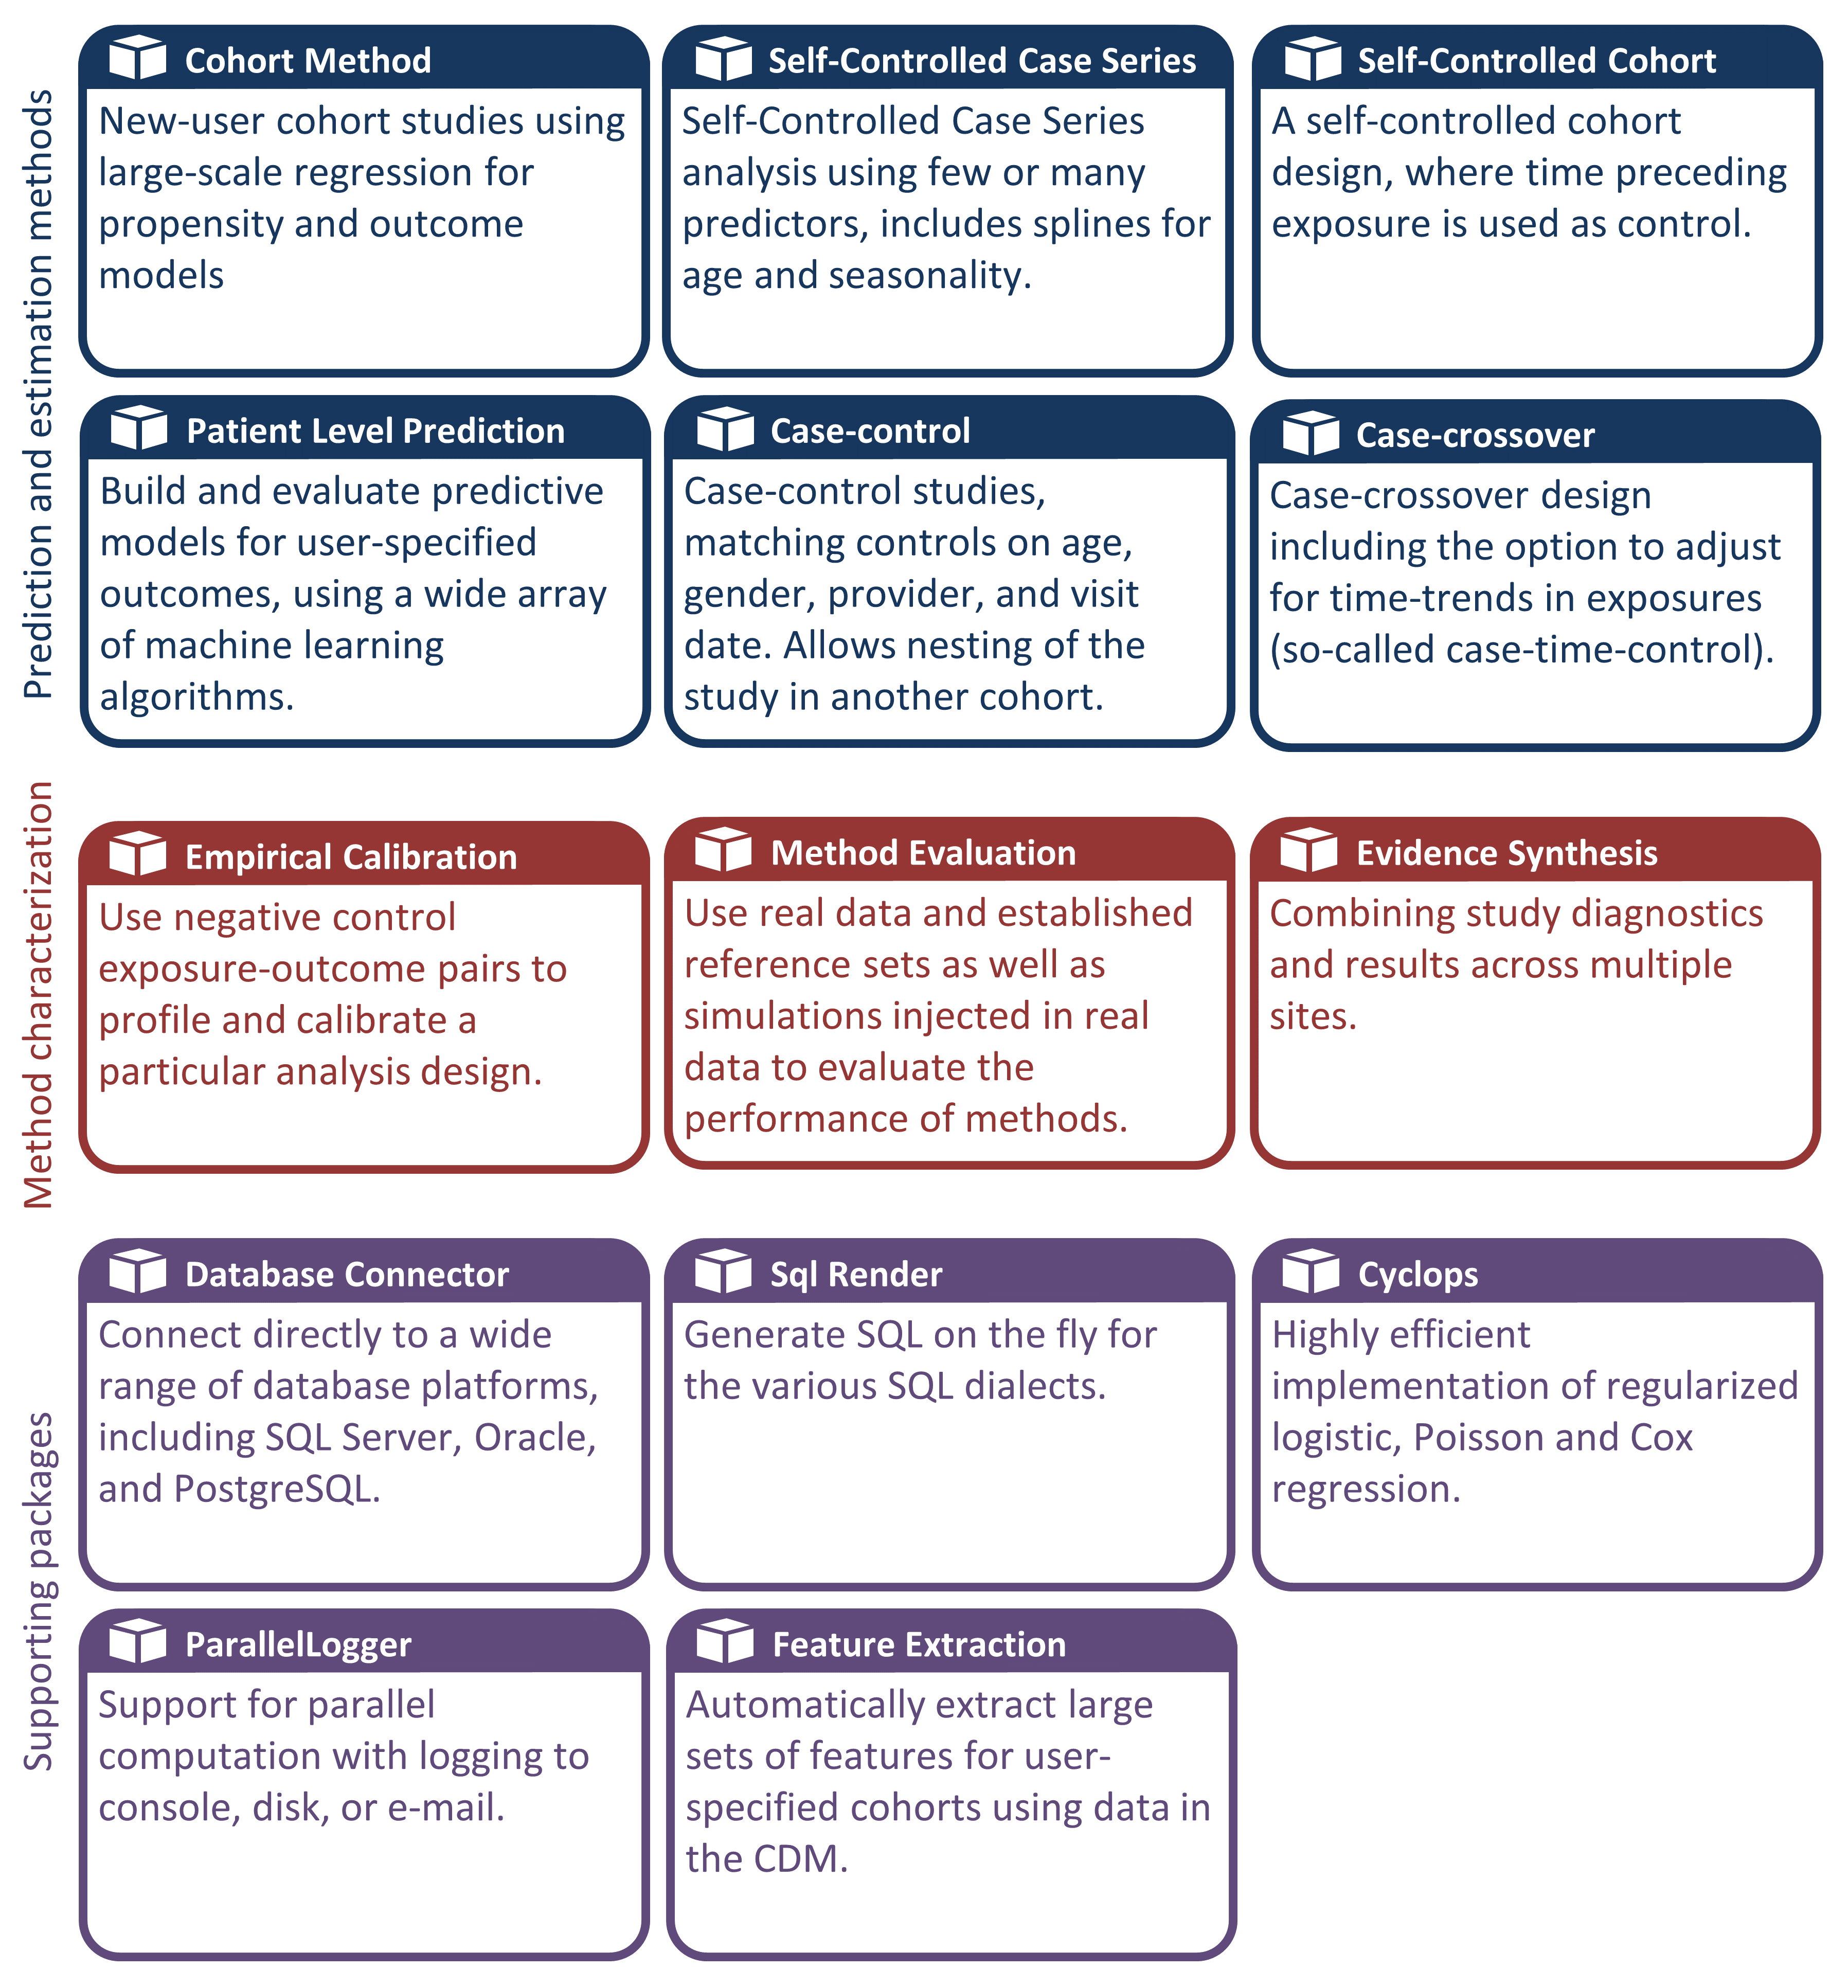
\includegraphics[width=1\linewidth]{images/OhdsiAnalyticsTools/methodsLibrary} 

}

\caption{OHDSI Methods Libraryのパッケージ}\label{fig:methodsLibrary}
\end{figure}

これらのパッケージは、CDM内のデータから始まり、推定値やそれを裏付ける統計、図表を生成する完全な観察研究を実施するためのR関数を提供しています。これらのパッケージはCDM内の観察データと直接やりとりし、第\ref{SqlAndR}章で説明されているような完全にカスタマイズされた分析にクロスプラットフォームの互換性を提供するために用いることも、集団特性の評価(第\ref{Characterization}章)、集団レベルの効果推定(第\ref{PopulationLevelEstimation}章)、患者レベルの予測(第\ref{PatientLevelPrediction}章 )のための高度な標準化分析を提供することもできます。Methods libraryは、透明性、再現性、異なるコンテキストでのメソッドの操作特性の測定値、そのメソッドによって生成される推定値やその後の経験的キャリブレーションなど、過去や現在の研究から学んだベストプラクティスをサポートしています。

Methods libraryはすでに多くの公表された臨床研究 \citep{boland_2017, duke_2017, ramcharran_2017, weinstein_2017, wang_2017, ryan_2017, ryan_2018, vashisht_2018, yuan_2018, johnston_2019} で使用されており、方法論の研究にも利用されています \citep{schuemie_2014, schuemie_2016, reps2018, tian_2018, schuemie_2018, schuemie_2018b, reps_2019}。Methods library内のメソッドの実装の妥当性については第 \ref{SoftwareValidity} 章で説明されています。

\subsection{大規模分析サポート}\label{ux5927ux898fux6a21ux5206ux6790ux30b5ux30ddux30fcux30c8}

すべてのパッケージで組み込まれている重要な機能の一つは、多くの分析を効率的に実行できることです。例えば、集団レベルの推定を行う場合、CohortMethodパッケージは多数の曝露とアウトカムに対して効果量の推定を行うことを可能にし、さまざまな分析設定を使用して、必要な中間データセットや最終データセットを計算するための最適な方法を自動的に選択します。共変量の抽出や、一つのターゲット・コンパレータペアに対して複数のアウトカムで使用される傾向スコアモデルの適合など、再利用可能なステップは一度だけ実行されます。可能な場合は、計算リソースを最大限に活用するために計算は並列処理われます。

この計算効率により、大規模な分析が可能になり、多くの質問に一度に回答することができます。また、コントロール仮説(ネガティブコントロールなど)を含めることで、当社の手法の運用特性を測定し、第\ref{MethodValidity} で説明されているように、経験則に基づくキャリブレーションを行うことも不可欠です。 \index{control hypotheses}

\subsection{ビッグデータ対応}\label{BigDataSupport}

Methods libraryは、非常に大規模なデータベースに対しても大量のデータを含む計算を実行できるようにデザインされています。これは次の三つの方法で実現されます:

\begin{enumerate}
\def\labelenumi{\arabic{enumi}.}
\tightlist
\item
  大部分のデータ操作はデータベースサーバー上で実行されます。分析は通常、データベース内の全データのごく一部しか必要としないため、Methods libraryはSqlRenderやDatabaseConnectorパッケージを介して関連データの前処理や抽出をする高度な操作をサーバー上で実行できるようにします。
\item
  大量のローカルデータオブジェクトはメモリ効率の良い方法で保存されます。ローカルマシンにダウンロードされるデータについては、Methods libraryは\href{https://cran.r-project.org/web/packages/ff}{ff}パッケージを使用して大規模データオブジェクトを保存、処理します。これにより、メモリに収まらないほど大きなデータでも処理することが可能です。
\item
  必要に応じて高性能コンピューティングが適用されます。例えば、\href{https://ohdsi.github.io/Cyclops/}{Cyclops}パッケージは、Methods library全体で使用される非常に効率的な回帰エンジンを実装しており、これにより通常は適合できない大規模な回帰(多くの変数、大量の観測値)を実行することができます。
\end{enumerate}

\subsection{ドキュメント}\label{ux30c9ux30adux30e5ux30e1ux30f3ux30c8-1}

Rはパッケージを文書化するための標準的な方法を提供しています。各パッケージには、パッケージに含まれるすべての関数とデータセットを文書化した\emph{パッケージマニュアル}があります。すべてのパッケージマニュアルは、Methods Libraryのウェブサイト\footnote{\url{https://ohdsi.github.io/MethodsLibrary}}、パッケージのGitHubリポジトリ、CRANで利用できます。さらに、Rの内部からパッケージマニュアルを参照するにはクエスチョンマークを使用します。例えばDatabaseConnectorパッケージを読み込んだ後、コマンド\texttt{?connect}を入力すると「connect」関数に関するドキュメントが表示されます。

パッケージマニュアルに加えて、多くのパッケージは\emph{ビネット}が提供されています。ビネットは、特定のタスクを実行するためにパッケージをどのように使用するかを説明した詳細なドキュメントです。例えば、一つのビネット\footnote{\url{https://ohdsi.github.io/CohortMethod/articles/MultipleAnalyses.html}}では、CohortMethodパッケージを使用して複数の分析を効率的に実行する方法が説明されています。ビネットはMethods Libraryのウェブサイト、パッケージのGitHubリポジトリ、CRANで入手可能なパッケージはCRANでも見つけることができます。 \index{vignette}

\subsection{システム要件}\label{ux30b7ux30b9ux30c6ux30e0ux8981ux4ef6}

システム要件を検討する際には、二つのコンピューティング環境が関連してきます:データベースサーバーと分析ワークステーションです。 \index{system requirements}

データベースサーバーはCDM形式の観察医療データを保持する必要があります。Methods libraryは、従来のデータベースシステム(PostgreSQL、Microsoft SQL Server、Oracle)、パラレルデータウェアハウス(Microsoft APS、IBM Netezza、Amazon Redshift)、に加えビッグデータプラットフォーム(Impala経由でのHadoop、Google BigQuery)など、幅広いデータベース管理システムをサポートしています。

分析ワークステーションは、Methods libraryがインストールされ実行される場所です。これがローカルマシン(例えば、ノートパソコン)か、RStudio Serverが実行されるリモートサーバーかに関わらず、Rがインストールされている必要があります。可能であればRStudioも一緒にインストールすることをお勧めします。また、Methods LibraryではJavaがインストールされている必要があります。分析ワークステーションはデータベースサーバーに接続できる必要があり、具体的には、両者の間にファイアウォールがある場合は、ワークステーションでデータベースサーバーのアクセスポートが開いている必要があります。一部の分析は計算集中的であるため、複数のプロセッサコアと十分なメモリを持つことが分析の高速化につながります。少なくとも4コアと16ギガバイトのメモリを推奨します。

\subsection{インストール方法}\label{installR}

OHDSI Rパッケージを実行するために必要な環境をインストールするための手順は次の通りです。インストールする必要があるものは4つあります: \index{R!installation}

\begin{enumerate}
\def\labelenumi{\arabic{enumi}.}
\tightlist
\item
  \textbf{R}は統計的コンピューティング環境です。基本的なユーザインターフェースとして主にコマンドラインインターフェースを提供します。
\item
  \textbf{Rtools}は、WindowsでRパッケージをソースからビルドする際に必要なプログラム一式です。
\item
  \textbf{RStudio}は、Rを使いやすくするIDE(統合開発環境)です。コードエディタ、デバッグ、およびビジュアルツールが含まれています。素晴らしいR体験を得るために、これを使用ください。
\item
  \textbf{Java}は、OHDSI Rパッケージの一部のコンポーネント、例えばデータベースへの接続に必要なコンポーネントを実行するために必要なコンピューティング環境です。
\end{enumerate}

以下では、Windows環境でのそれぞれのインストール方法を説明します。

\begin{rmdimportant}
Windowsでは、RとJavaはどちらも32ビットと64ビットのアーキテクチャがあります。Rを両方のアーキテクチャにインストールする場合、Javaも両方のアーキテクチャにインストールしなければなりません。Rの64ビットのみをインストールすることをお勧めします。
\end{rmdimportant}

\subsubsection*{Rのインストール}\label{rux306eux30a4ux30f3ux30b9ux30c8ux30fcux30eb}
\addcontentsline{toc}{subsubsection}{Rのインストール}

\begin{enumerate}
\def\labelenumi{\arabic{enumi}.}
\tightlist
\item
  \url{https://cran.r-project.org/} で、図 \ref{fig:downloadR} に示されるように「Download R for Windows 」、「base」 の順にクリックし、ダウンロードしてください。
\end{enumerate}

\begin{figure}

{\centering 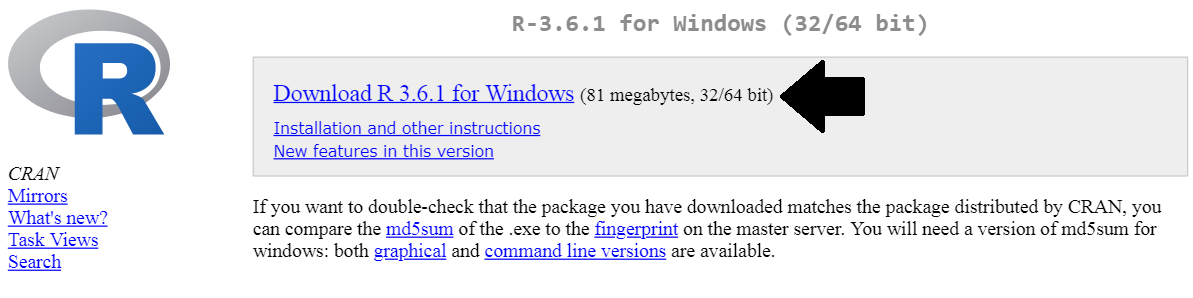
\includegraphics[width=1\linewidth]{images/OhdsiAnalyticsTools/downloadR} 

}

\caption{CRANからのRのダウンロード}\label{fig:downloadR}
\end{figure}

\begin{enumerate}
\def\labelenumi{\arabic{enumi}.}
\setcounter{enumi}{1}
\tightlist
\item
  ダウンロードが完了したら、インストーラを実行します。2つの例外を除いて、すべてデフォルトのオプションを使用してください: まず、プログラムファイルにはインストールしない方が良いでしょう。代わりに、図 \ref{fig:rDestination} のように、CドライブのサブフォルダとしてRを作成します。次に、RとJavaのアーキテクチャの違いによる問題を回避するため、図 \ref{fig:no32Bits} のように32ビットアーキテクチャを無効にします。
\end{enumerate}

\begin{figure}

{\centering 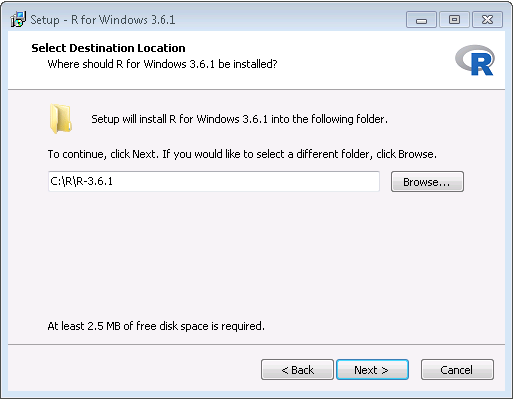
\includegraphics[width=0.8\linewidth]{images/OhdsiAnalyticsTools/rDestination} 

}

\caption{Rフォルダの設定}\label{fig:rDestination}
\end{figure}

\begin{figure}

{\centering 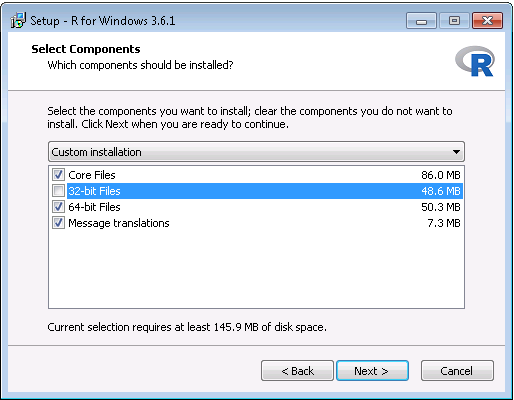
\includegraphics[width=0.8\linewidth]{images/OhdsiAnalyticsTools/no32Bits} 

}

\caption{32ビットバージョンのRを無効化}\label{fig:no32Bits}
\end{figure}

完了すると、スタートメニューからRを選択できるようになります。

\subsubsection*{Rtoolsのインストール}\label{rtoolsux306eux30a4ux30f3ux30b9ux30c8ux30fcux30eb}
\addcontentsline{toc}{subsubsection}{Rtoolsのインストール}

\begin{enumerate}
\def\labelenumi{\arabic{enumi}.}
\item
  \url{https://cran.r-project.org/} にアクセスし、「Download R for Windows」をクリックし、次に「Rtools」をクリックして、最新版のRtoolsをダウンロードします。
\item
  ダウンロードが完了後、インストーラを実行します。すべてデフォルトのオプションを選択します。
\end{enumerate}

\subsubsection*{RStudioのインストール}\label{rstudioux306eux30a4ux30f3ux30b9ux30c8ux30fcux30eb}
\addcontentsline{toc}{subsubsection}{RStudioのインストール}

\begin{enumerate}
\def\labelenumi{\arabic{enumi}.}
\tightlist
\item
  \url{https://www.rstudio.com/} にアクセスし、「Download RStudio」またはRStudioの下の「ダウンロード」ボタンをクリックし、無料版を選択し、図 \ref{fig:downloadRStudio} に示されるようにWindows用のインストーラをダウンロードします。
\end{enumerate}

\begin{figure}

{\centering 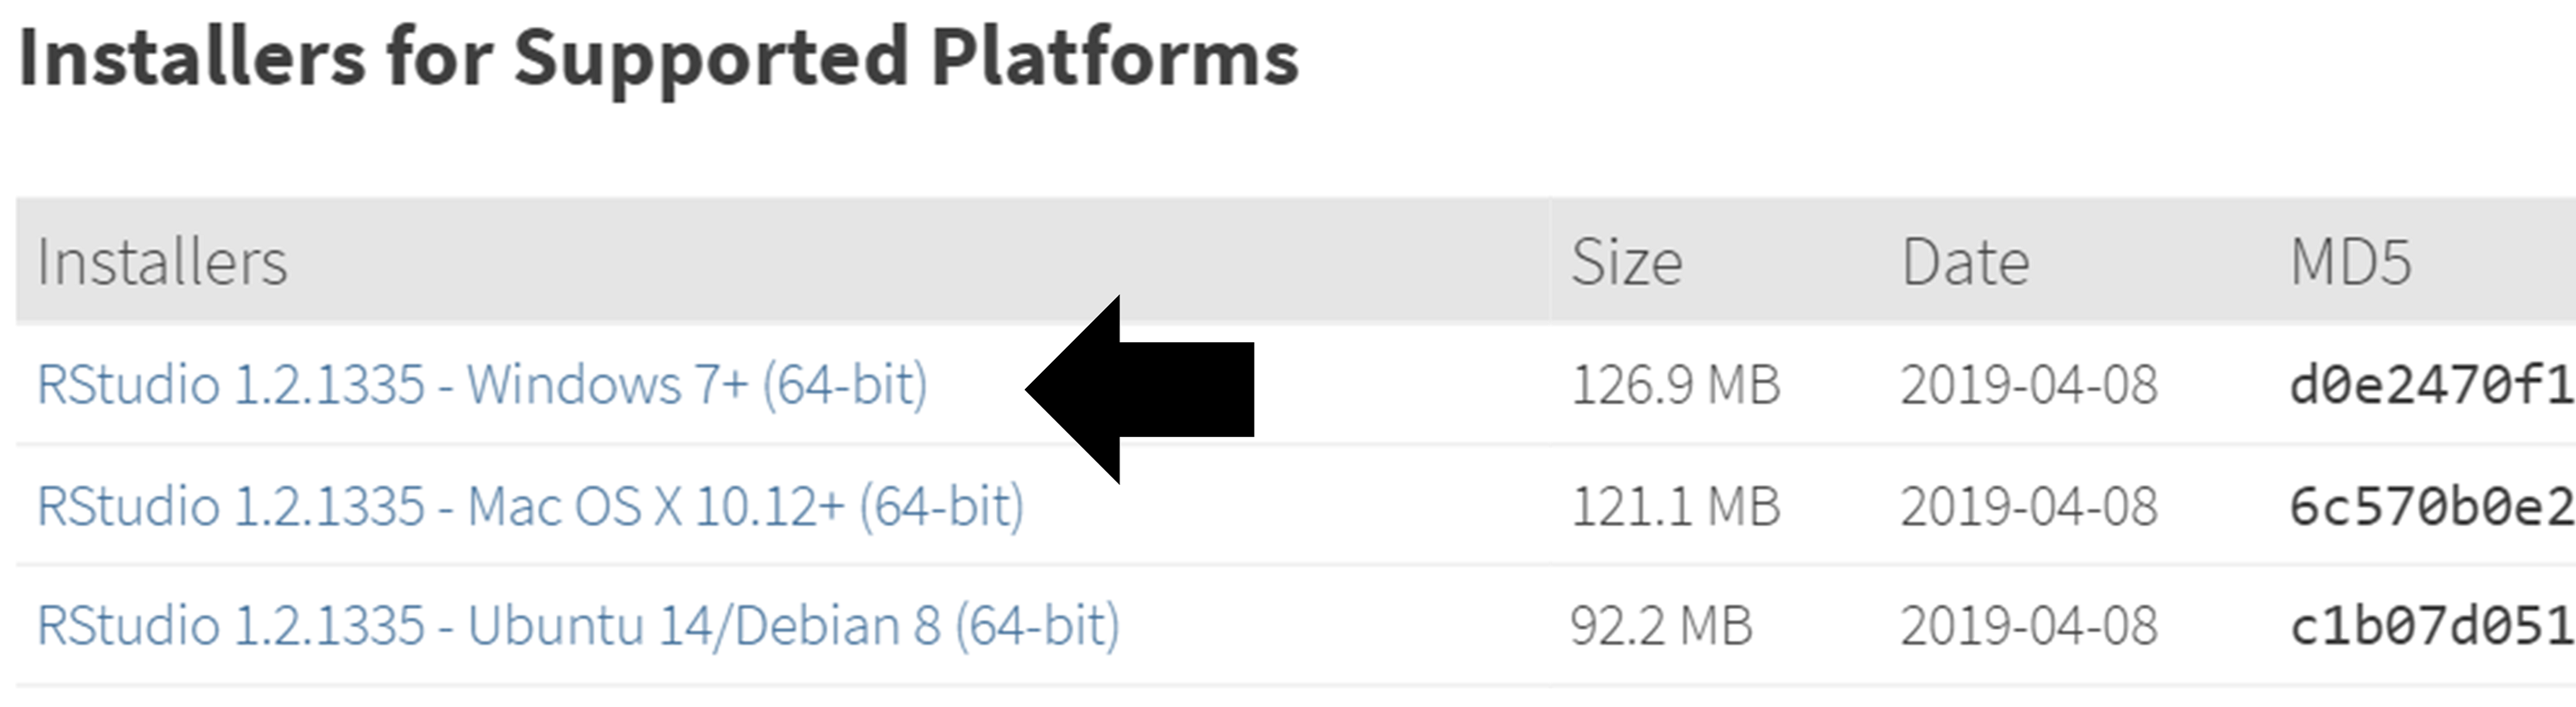
\includegraphics[width=1\linewidth]{images/OhdsiAnalyticsTools/downloadRStudio} 

}

\caption{RStudioのダウンロード}\label{fig:downloadRStudio}
\end{figure}

\begin{enumerate}
\def\labelenumi{\arabic{enumi}.}
\setcounter{enumi}{1}
\tightlist
\item
  ダウンロードが完了後、インストーラを実行します。すべてデフォルトのオプションを選択してください。
\end{enumerate}

\subsubsection*{Javaのインストール}\label{javaux306eux30a4ux30f3ux30b9ux30c8ux30fcux30eb}
\addcontentsline{toc}{subsubsection}{Javaのインストール}

\begin{enumerate}
\def\labelenumi{\arabic{enumi}.}
\tightlist
\item
  \url{https://java.com/en/download/manual.jsp} にアクセスし、図 \ref{fig:downloadJava} に示されるように、Wiindows64ビット版のインストーラを選択します。32ビット版のRもインストールしている場合には、Javaも32ビット版をインストールしなければなりません。
\end{enumerate}

\begin{figure}

{\centering 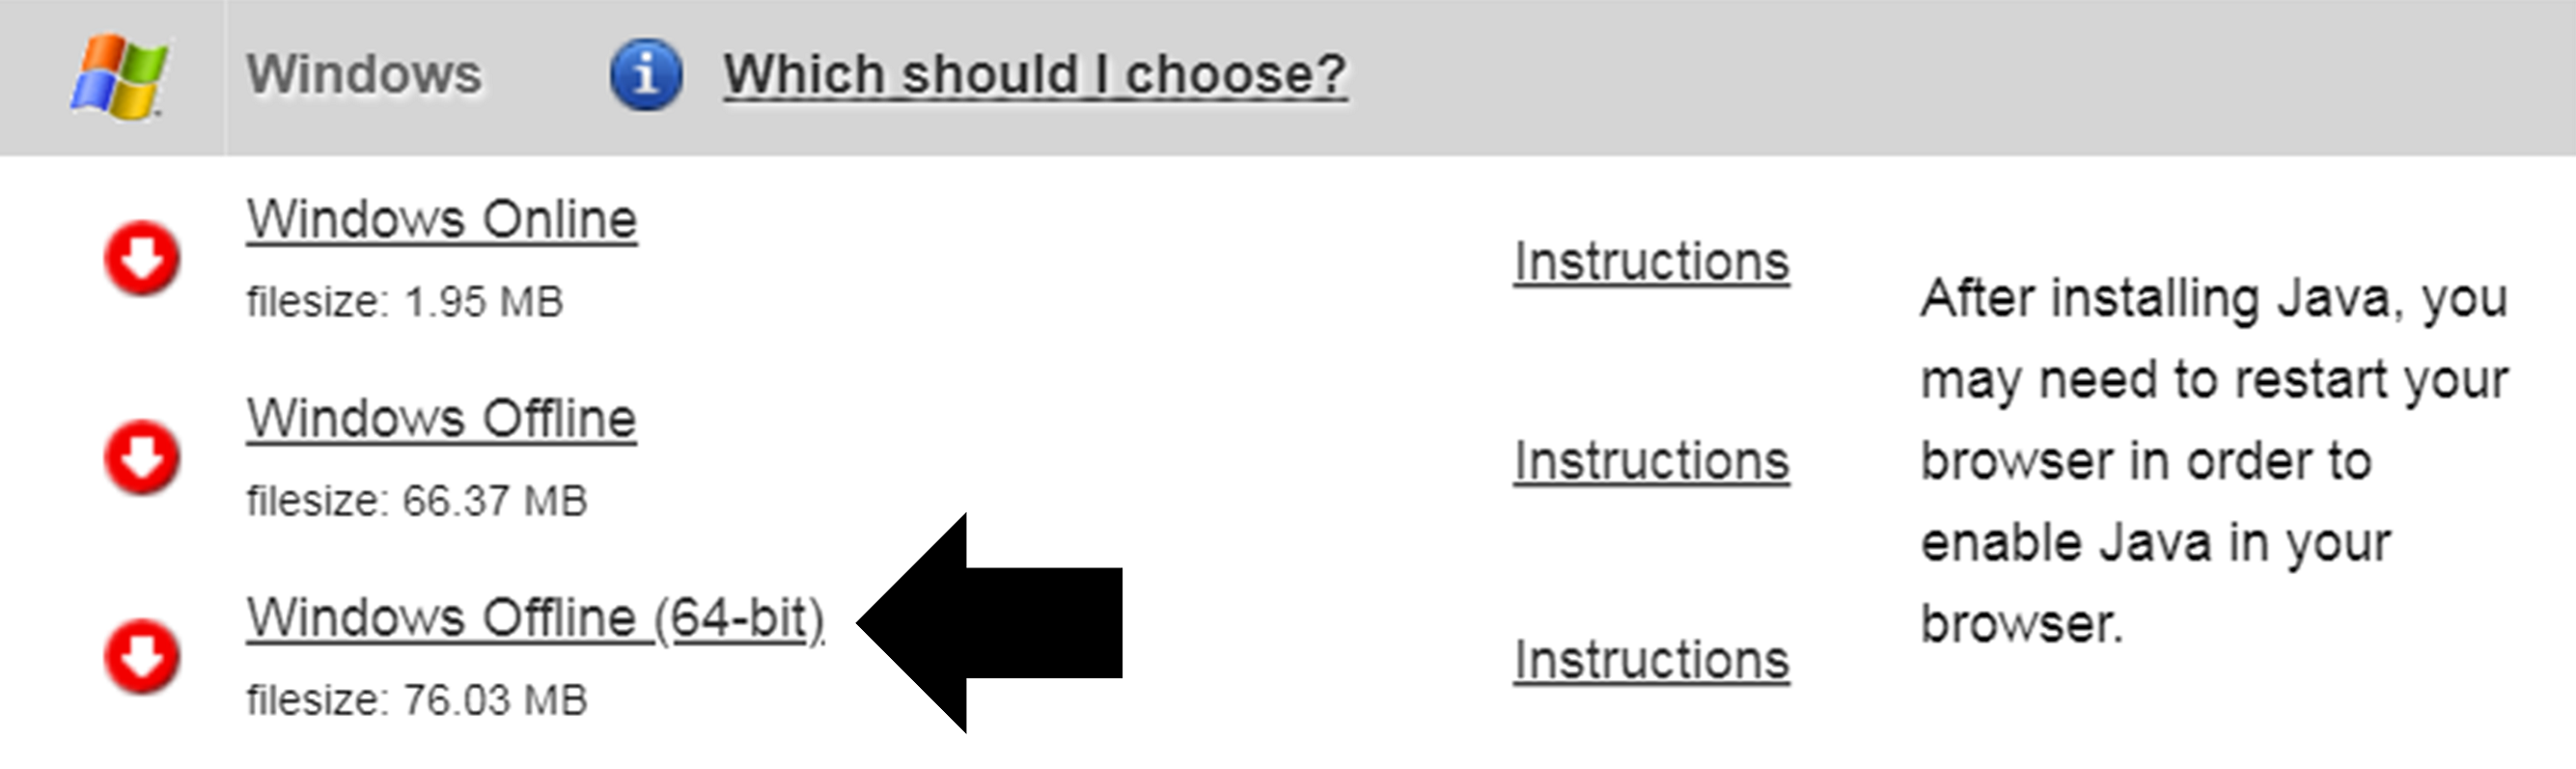
\includegraphics[width=1\linewidth]{images/OhdsiAnalyticsTools/downloadJava} 

}

\caption{Javaのダウンロード}\label{fig:downloadJava}
\end{figure}

\begin{enumerate}
\def\labelenumi{\arabic{enumi}.}
\setcounter{enumi}{1}
\tightlist
\item
  ダウンロード後、インストーラを実行してます。
\end{enumerate}

\subsubsection*{インストールの確認}\label{ux30a4ux30f3ux30b9ux30c8ux30fcux30ebux306eux78baux8a8d}
\addcontentsline{toc}{subsubsection}{インストールの確認}

これで準備は整ったはずですが、念のため確認しておきましょう。Rを起動し、下記のようにタイプしてください。

\begin{Shaded}
\begin{Highlighting}[]
\FunctionTok{install.packages}\NormalTok{(}\StringTok{"SqlRender"}\NormalTok{)}
\FunctionTok{library}\NormalTok{(SqlRender)}
\FunctionTok{translate}\NormalTok{(}\StringTok{"SELECT TOP 10 * FROM person;"}\NormalTok{, }\StringTok{"postgresql"}\NormalTok{)}
\end{Highlighting}
\end{Shaded}

\begin{verbatim}
## [1] "SELECT  * FROM person LIMIT 10;"
## attr(,"sqlDialect")
## [1] "postgresql"
\end{verbatim}

この関数はJavaを使用するので、すべてがうまくいけば、RとJavaの両方が正しくインストールされていることがわかります!

もう一つのテストは、ソースパッケージがビルドできるかどうかを確認することです。以下のRコードを実行して、OHDSI GitHubリポジトリから\texttt{CohortMethod}パッケージをインストールします:

\begin{Shaded}
\begin{Highlighting}[]
\FunctionTok{install.packages}\NormalTok{(}\StringTok{"drat"}\NormalTok{)}
\NormalTok{drat}\SpecialCharTok{::}\FunctionTok{addRepo}\NormalTok{(}\StringTok{"OHDSI"}\NormalTok{)}
\FunctionTok{install.packages}\NormalTok{(}\StringTok{"CohortMethod"}\NormalTok{)}
\end{Highlighting}
\end{Shaded}

\section{展開戦略}\label{ux5c55ux958bux6226ux7565}

ATLASやMethods Libraryを含むOHDSIツールスタック全体を組織内で展開することは、非常に困難な作業です。依存関係がある多くのコンポーネントを考慮し、設定を行う必要があります。このため、二つの取り組みが、スタック全体を一つのパッケージとしてインストールできる統合展開戦略を開発しました。一部の仮想化技術を使用して、これを実現します。それは、BroadseaおよびAmazon Web Services (AWS)です。 \index{tools deployment}

\subsection{Broadsea}\label{broadsea}

Broadsea\footnote{\url{https://github.com/OHDSI/Broadsea}}はDockerコンテナ技術\footnote{\url{https://www.docker.com/}}を使用しています。OHDSIツールは依存関係とともに、Dockerイメージと呼ばれる単一のポータブルなバイナリファイルにパッケージ化されています。このイメージはDockerエンジンサービス上で実行でき、すべてのソフトウェアがインストールされるとすぐに実行可能な仮想マシンが作成されます。DockerエンジンはMicrosoft Windows、MacOS、Linuxなどのほとんどのオペレーティングシステムで利用可能です。Broadsea Dockerイメージには、Methods libraryやATLASを含む主なOHDSIツールが含まれています。 \index{tools deployment!Broadsea}

\subsection{Amazon AWS}\label{amazon-aws}

Amazonは、AWSクラウドコンピューティング環境でボタンをクリックするだけでインスタンス化できる二つの環境を用意しています:OHDSI-in-a-Box\footnote{\url{https://github.com/OHDSI/OHDSI-in-a-Box}}とOHDSIonAWS\footnote{\url{https://github.com/OHDSI/OHDSIonAWS}}です。 \index{tools deployment!Amazon AWS}

OHDSI-in-a-Boxは特に学習環境として作成さたものであり、OHDSIコミュニティが提供するほとんどのチュートリアルで使用されています。これには多くのOHDSIツール、サンプルデータセット、RStudio、その他のサポートソフトウェアが低コストの単一のWindows仮想マシンに含まれています。PostgreSQLデータベースは、CDMの保存と、ATLASからの中間結果の保存の両方に使用されます。OMOP CDMデータマッピングとETLツールも、OHDSI-in-a-Boxに含まれています。OHDSI-in-a-Boxのアーキテクチャは、図 \ref{fig:ohdsiinaboxDiagram} に示されています。

\begin{figure}

{\centering 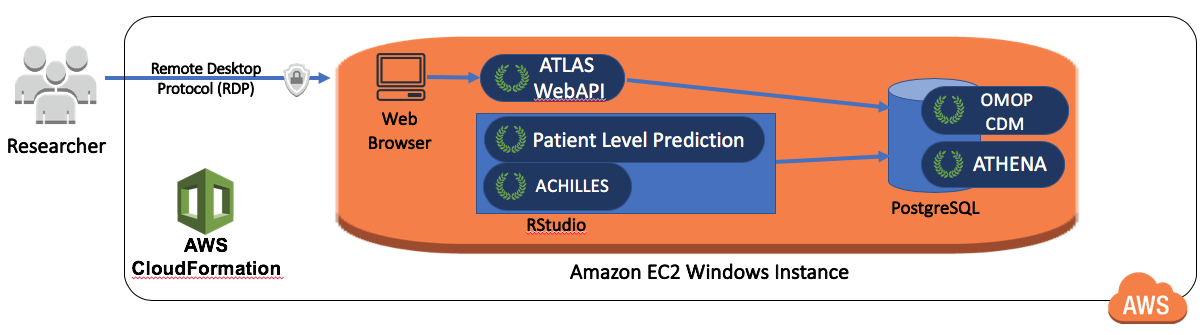
\includegraphics[width=1\linewidth]{images/OhdsiAnalyticsTools/OHDSI-in-a-BoxDiagram} 

}

\caption{OHDSI-in-a-BoxのAmazon Web Servicesアーキテクチャ}\label{fig:ohdsiinaboxDiagram}
\end{figure}

OHDSIonAWSは、企業向け、マルチユーザー対応、拡張性や耐障害性に優れたOHDSI環境のためのリファレンスアーキテクチャであり、組織がデータ分析を行う際に使用することができます。 複数のサンプルデータセットが含まれており、組織の実際のヘルスケアデータを自動的にロードすることも可能です。 データはAmazon Redshiftデータベースプラットフォームに配置され、OHDSIツールによってサポートされます。 ATLASの中間結果はPostgreSQLデータベースに保存されます。ユーザーはフロントエンドで、ウェブインターフェース(RStudio Serverを活用)を通じてATLASやRStudioにアクセスできます。RStudioにはOHDSI Methods Libraryがすでにインストールされており、データベースへの接続に使用できます。OHDSIonAWSの自動展開はオープンソースであり、組織の管理ツールやベストプラクティスを含めるようにカスタマイズできます。OHDSIonAWSのアーキテクチャは図\ref{fig:ohdsionawsDiagram}に示されています。

\begin{figure}

{\centering 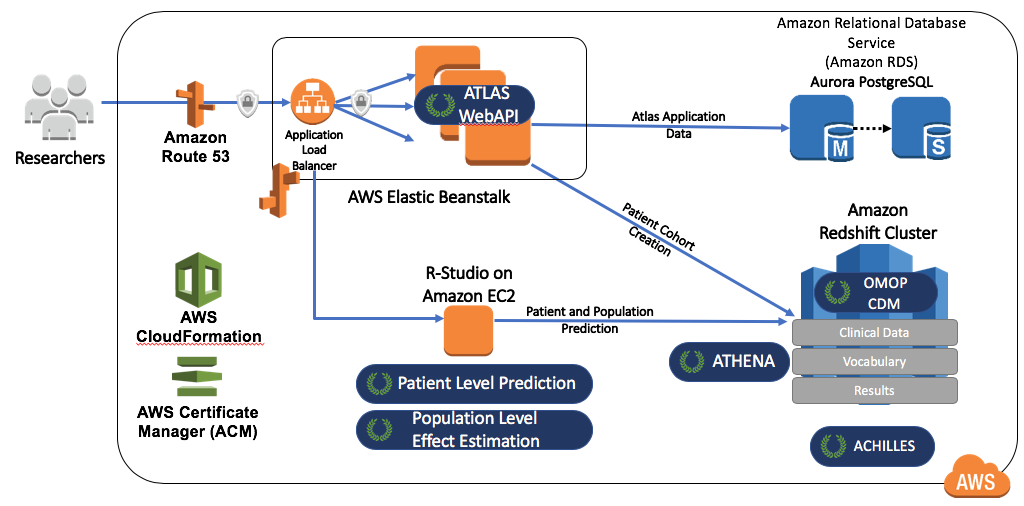
\includegraphics[width=1\linewidth]{images/OhdsiAnalyticsTools/OHDSIonAWSDiagram} 

}

\caption{OHDSIonAWSのAmazon Web Servicesアーキテクチャ}\label{fig:ohdsionawsDiagram}
\end{figure}

\section{まとめ}\label{ux307eux3068ux3081-6}

\begin{rmdsummary}
\begin{itemize}
\tightlist
\item
  CDM内のデータに対して分析を行うには

  \begin{itemize}
  \tightlist
  \item
    カスタムコードを作成する
  \item
    OHDSI Methods LibraryのRパッケージを使用したコードを作成する
  \item
    インタラクティブな分析プラットフォームATLASを使用する
  \end{itemize}
\item
  OHDSIツールはさまざまな分析戦略を用いています

  \begin{itemize}
  \tightlist
  \item
    単一研究
  \item
    リアルタイムクエリ
  \item
    大規模アナリティクス
  \end{itemize}
\item
  OHDSIアナリティクスツールのほとんどは、以下に組み込まれています

  \begin{itemize}
  \tightlist
  \item
    インタラクティブな分析プラットフォームATLAS
  \item
    OHDSI Methods LibraryのRパッケージ
  \end{itemize}
\item
  OHDSIツールの展開を容易にするいくつかの戦略があります。
\end{itemize}
\end{rmdsummary}

\chapter{--翻訳作業中-- SQLとR}\label{SqlAndR}

\emph{著者: Martijn Schuemie \& Peter Rijnbeek}

共通データモデル(CDM)はリレーショナルデータベースモデルです(すべてのデータはフィールドを持つテーブルのレコードとして表されます)。そのため、データは通常、PostgreSQL、Oracle、Microsoft SQL Serverなどのソフトウェアプラットフォームを使用してリレーショナルデータベースに保存されます。ATLASやMethods LibraryなどのさまざまなOHDSIツールは、バックグラウンドでデータベースにクエリを出すことで動作しますが、適切なアクセス権があれば、私たちも自身も直接データベースにクエリを出すことができます。その主な理由は、現在のツールではサポートされていない分析を行うためです。ただし、OHDSI ツールは多くの場合、ユーザーがデータを適切に分析できるよう、ガイドするように設計されているため、データベースを直接クエリすると、間違いを犯すリスクも高くなります。直接のクエリでは、そのようなガイドは提供されていません。

リレーショナルデータベースをクエリする標準的な言語はSQL(Structured Query Language)で、クエリやデータ変更に使用できます。 SQLの基本コマンドは確かに標準化されており、ソフトウェアプラットフォーム間で同じ意味を持ちますが、各プラットフォームには独自の「方言」があり、微妙な違いがあります。 例えば、SQL Server上のPERSONテーブルの最初の10行を取得するには、次のように入力します。: \index{SQL} \index{structured query language|see {SQL}}

\begin{Shaded}
\begin{Highlighting}[]
\KeywordTok{SELECT}\NormalTok{ TOP }\DecValTok{10} \OperatorTok{*} \KeywordTok{FROM}\NormalTok{ person;}
\end{Highlighting}
\end{Shaded}

一方、PostgreSQLでは同じクエリは次のようになります:

\begin{Shaded}
\begin{Highlighting}[]
\KeywordTok{SELECT} \OperatorTok{*} \KeywordTok{FROM}\NormalTok{ person }\KeywordTok{LIMIT} \DecValTok{10}\NormalTok{;}
\end{Highlighting}
\end{Shaded}

OHDSIでは、プラットフォーム固有の表現に依存しないことを望んでいます。すなわち、すべてのOHDSIデータベースで同じSQL言語を使用したいと考えています。このため、OHDSIは\href{https://ohdsi.github.io/SqlRender/}{SqlRender}パッケージを開発しました。これは、ある標準の表現から後述するサポート対象の表現に翻訳できるRパッケージです。この標準表現である - \textbf{OHDSI SQL} - は主にSQL Server SQL表現のサブセットです。本章で例示するSQL文はすべてOHDSI SQLを使用します。 \index{SqlRender} \index{agnostic SQL|see {SqlRender}} \index{Standard SQL Dialect|see {SqlRender}} \index{OHDSI SQL|see {SqlRender}}

各データベースプラットフォームには、SQLを使用したデータベースのクエリのための独自のソフトウェアツールも付属しています。OHDSIでは、多くのデータベースプラットフォームに接続できるRパッケージ、\href{https://ohdsi.github.io/DatabaseConnector/}{DatabaseConnector}パッケージを開発しました。DatabaseConnectorも本章の後半で説明します。 \index{DatabaseConnector}

そのため、CDMに準拠したデータベースに対してOHDSIツールを使用せずにクエリを実行できますが、推奨されるパスはDatabaseConnectorとSqlRenderパッケージを使用することです。これにより、あるサイトで開発されたクエリが他のサイトでも修正することなく使用できるようになります。R自体も、データベースから抽出されたデータをさらに分析する機能を提供しており、統計分析の実行や(インタラクティブな)プロットの生成などが可能です。 \index{R}

本章では、読者がSQLの基本的な理解をしていることを前提としています。まず、SqlRenderとDatabaseConnectorの使用方法を確認します。これらのパッケージを使用しない場合は、このセクションをスキップいただいて構いません。セクション\ref{QueryTheCdm} では、CDMにクエリを出すためのSQL(この場合OHDSI SQL)を使用する方法を説明します。次のセクションでは、CDMにクエリする際にOHDSI標準化ボキャブラリを使用する方法を説明します。CDMに対する一般的に使用されるクエリのコレクションであり、一般に公開されているQueryLibraryに焦点を当てます。本章の最後では、発生率を推定する研究例を取り上げ、SqlRenderとDatabaseConnectorを使用してこの研究を実施します。 \index{Query Library} \index{SQL Query Library|see {Query Library}}

\section{SqlRender}\label{SqlRender}

\href{https://ohdsi.github.io/SqlRender/}{SqlRender} パッケージは CRAN(Comprehensive R Archive Network)で入手可能であり、以下のコマンドでインストールできます:

\begin{Shaded}
\begin{Highlighting}[]
\FunctionTok{install.packages}\NormalTok{(}\StringTok{"SqlRender"}\NormalTok{)}
\end{Highlighting}
\end{Shaded}

SqlRenderは、従来のデータベースシステム(PostgreSQL、Microsoft SQL Server、SQLite、Oracle)や並列データウェアハウス(Microsoft APS、IBM Netezza、Amazon Redshift)に加え、ビッグデータプラットフォーム(Hadoop から Impala、Google BigQuery)など、幅広い技術プラットフォームをサポートしています。Rパッケージには、パッケージマニュアルと、全機能を紹介するビネットが付属しています。ここでは、主な機能の一部を紹介します。

\subsection{SQLのパラメータ設定}\label{sqlux306eux30d1ux30e9ux30e1ux30fcux30bfux8a2dux5b9a}

パッケージの機能のひとつは、SQLのパラメータ化をサポートすることです。 しばしば、いくつかのパラメータに基づいて、SQLの小さなバリエーションを生成する必要があります。SqlRenderは、SQLコード内にシンプルなマークアップ構文を提供し、パラメータ化を可能にします。パラメータ値に基づくSQLのレンダリングは、\texttt{render()}関数を使用して行います。\index{SqlRender!parameterization}

\subsubsection*{パラメータ値の置換}\label{ux30d1ux30e9ux30e1ux30fcux30bfux5024ux306eux7f6eux63db}
\addcontentsline{toc}{subsubsection}{パラメータ値の置換}

\texttt{@} 文字を使用して、レンダリング時に実際のパラメータ値と置換する必要があるパラメータ名を示します。以下の例では、SQL内で \texttt{a} という変数がSQLで言及されています。\texttt{render} 関数の呼び出しでは、このパラメータの値が定義されています:

\begin{Shaded}
\begin{Highlighting}[]
\NormalTok{sql }\OtherTok{\textless{}{-}} \StringTok{"SELECT * FROM concept WHERE concept\_id = @a;"}
\FunctionTok{render}\NormalTok{(sql, }\AttributeTok{a =} \DecValTok{123}\NormalTok{)}
\end{Highlighting}
\end{Shaded}

\begin{verbatim}
## [1] "SELECT * FROM concept WHERE concept_id = 123;"
\end{verbatim}

ほとんどのデータベース管理システムが提供するパラメータ化とは異なり、テーブル名やフィールド名を値と同様に簡単にパラメータ化できることに注目ください。:

\begin{Shaded}
\begin{Highlighting}[]
\NormalTok{sql }\OtherTok{\textless{}{-}} \StringTok{"SELECT * FROM @x WHERE person\_id = @a;"}
\FunctionTok{render}\NormalTok{(sql, }\AttributeTok{x =} \StringTok{"observation"}\NormalTok{, }\AttributeTok{a =} \DecValTok{123}\NormalTok{)}
\end{Highlighting}
\end{Shaded}

\begin{verbatim}
## [1] "SELECT * FROM observation WHERE person_id = 123;"
\end{verbatim}

パラメータ値は、数値、文字列、ブーリアン変数、ベクトル(カンマ区切りのリストに変換される)とすることができます。:

\begin{Shaded}
\begin{Highlighting}[]
\NormalTok{sql }\OtherTok{\textless{}{-}} \StringTok{"SELECT * FROM concept WHERE concept\_id IN (@a);"}
\FunctionTok{render}\NormalTok{(sql, }\AttributeTok{a =} \FunctionTok{c}\NormalTok{(}\DecValTok{123}\NormalTok{, }\DecValTok{234}\NormalTok{, }\DecValTok{345}\NormalTok{))}
\end{Highlighting}
\end{Shaded}

\begin{verbatim}
## [1] "SELECT * FROM concept WHERE concept_id IN (123,234,345);"
\end{verbatim}

\subsubsection*{If-Then-Else}\label{if-then-else}
\addcontentsline{toc}{subsubsection}{If-Then-Else}

時には、1つまたは複数のパラメータの値に基づいてコードブロックをオンまたはオフにする必要があります。これは、\texttt{\{Condition\}\ ?\ \{if\ true\}\ :\ \{if\ false\}} 構文を使用して行います。\emph{condition} が true または 1 の場合、\emph{if true} ブロックが使用され、それ以外の場合は \emph{if false} ブロックが(存在する場合)表示されます。

\begin{Shaded}
\begin{Highlighting}[]
\NormalTok{sql }\OtherTok{\textless{}{-}} \StringTok{"SELECT * FROM cohort \{@x\} ? \{WHERE subject\_id = 1\}"}
\FunctionTok{render}\NormalTok{(sql, }\AttributeTok{x =} \ConstantTok{FALSE}\NormalTok{)}
\end{Highlighting}
\end{Shaded}

\begin{verbatim}
## [1] "SELECT * FROM cohort "
\end{verbatim}

\begin{Shaded}
\begin{Highlighting}[]
\FunctionTok{render}\NormalTok{(sql, }\AttributeTok{x =} \ConstantTok{TRUE}\NormalTok{)}
\end{Highlighting}
\end{Shaded}

\begin{verbatim}
## [1] "SELECT * FROM cohort WHERE subject_id = 1"
\end{verbatim}

簡単な比較もサポートされています:

\begin{Shaded}
\begin{Highlighting}[]
\NormalTok{sql }\OtherTok{\textless{}{-}} \StringTok{"SELECT * FROM cohort \{@x == 1\} ? \{WHERE subject\_id = 1\};"}
\FunctionTok{render}\NormalTok{(sql, }\AttributeTok{x =} \DecValTok{1}\NormalTok{)}
\end{Highlighting}
\end{Shaded}

\begin{verbatim}
## [1] "SELECT * FROM cohort WHERE subject_id = 1;"
\end{verbatim}

\begin{Shaded}
\begin{Highlighting}[]
\FunctionTok{render}\NormalTok{(sql, }\AttributeTok{x =} \DecValTok{2}\NormalTok{)}
\end{Highlighting}
\end{Shaded}

\begin{verbatim}
## [1] "SELECT * FROM cohort ;"
\end{verbatim}

\texttt{IN} 演算子もサポートされています:

\begin{Shaded}
\begin{Highlighting}[]
\NormalTok{sql }\OtherTok{\textless{}{-}} \StringTok{"SELECT * FROM cohort \{@x IN (1,2,3)\} ? \{WHERE subject\_id = 1\};"}
\FunctionTok{render}\NormalTok{(sql, }\AttributeTok{x =} \DecValTok{2}\NormalTok{)}
\end{Highlighting}
\end{Shaded}

\begin{verbatim}
## [1] "SELECT * FROM cohort WHERE subject_id = 1;"
\end{verbatim}

\subsection{他のSQL表現への置換}\label{ux4ed6ux306esqlux8868ux73feux3078ux306eux7f6eux63db}

\href{https://ohdsi.github.io/SqlRender/}{SqlRender} パッケージのもう一つの機能は、OHDSI SQLから他のSQL表現へ変換することです。例えば:

\begin{Shaded}
\begin{Highlighting}[]
\NormalTok{sql }\OtherTok{\textless{}{-}} \StringTok{"SELECT TOP 10 * FROM person;"}
\FunctionTok{translate}\NormalTok{(sql, }\AttributeTok{targetDialect =} \StringTok{"postgresql"}\NormalTok{)}
\end{Highlighting}
\end{Shaded}

\begin{verbatim}
## [1] "SELECT  * FROM person LIMIT 10;"
## attr(,"sqlDialect")
## [1] "postgresql"
\end{verbatim}

\texttt{targetDialect} パラメータには次の値が設定可能です:``oracle'', ``postgresql'', ``pdw'', ``redshift'', ``impala'', ``netezza'', ``bigquery'', ``sqlite'', ``sql server''。 \index{SqlRender!translation}

\begin{rmdimportant}
SQL関数や構文を適切に変換できる範囲には限界があります。その理由は、パッケージには限られた数の変換ルールしか実装されていないことと、一部のSQL機能にはすべての方言に相当するものがないことが挙げられます。これが、OHDSI SQLが独自の新しいSQL方言として開発された主な理由です。しかし、可能な限り、車輪の再発明を避けるためにSQL Serverの構文に従うようにしています。
\end{rmdimportant}

最大限の努力を尽くしても、サポートされているすべてのプラットフォーム上でエラーなく実行されるOHDSI SQLを記載するには、考慮すべき点がいくつかあります。以下では、これらの考慮事項について詳しく説明します。

\subsubsection*{Translateがサポートする関数と構造}\label{translateux304cux30b5ux30ddux30fcux30c8ux3059ux308bux95a2ux6570ux3068ux69cbux9020}
\addcontentsline{toc}{subsubsection}{Translateがサポートする関数と構造}

これらのSQL Server関数はテスト済であり、各表現への正確な変換が確認されています:\index{SqlRender!supported functions}

\begin{longtable}[]{@{}lll@{}}
\caption{\label{tab:sqlFunctions} ``translate (翻訳)によりサポートされる関数と構造}\tabularnewline
\toprule\noalign{}
関数 & 関数 & 関数 \\
\midrule\noalign{}
\endfirsthead
\toprule\noalign{}
関数 & 関数 & 関数 \\
\midrule\noalign{}
\endhead
\bottomrule\noalign{}
\endlastfoot
ABS & EXP & RAND \\
ACOS & FLOOR & RANK \\
ASIN & GETDATE & RIGHT \\
ATAN & HASHBYTES* & ROUND \\
AVG & ISNULL & ROW\_NUMBER \\
CAST & ISNUMERIC & RTRIM \\
CEILING & LEFT & SIN \\
CHARINDEX & LEN & SQRT \\
CONCAT & LOG & SQUARE \\
COS & LOG10 & STDEV \\
COUNT & LOWER & SUM \\
COUNT\_BIG & LTRIM & TAN \\
DATEADD & MAX & UPPER \\
DATEDIFF & MIN & VAR \\
DATEFROMPARTS & MONTH & YEAR \\
DATETIMEFROMPARTS & NEWID & \\
DAY & PI & \\
EOMONTH & POWER & \\
\end{longtable}

* Oracleでは特別な権限が必要です。SQLiteでは同等のものがありません。

同様に、多くのSQL構文構造がサポートされています。以下は、正確に翻訳されることが確認されている非網羅的なリストです:

\begin{Shaded}
\begin{Highlighting}[]
\CommentTok{{-}{-} Simple selects:}
\KeywordTok{SELECT} \OperatorTok{*} \KeywordTok{FROM} \KeywordTok{table}\NormalTok{;}

\CommentTok{{-}{-} Selects with joins:}
\KeywordTok{SELECT} \OperatorTok{*} \KeywordTok{FROM}\NormalTok{ table\_1 }\KeywordTok{INNER} \KeywordTok{JOIN}\NormalTok{ table\_2 }\KeywordTok{ON}\NormalTok{ a }\OperatorTok{=}\NormalTok{ b;}

\CommentTok{{-}{-} Nested queries:}
\KeywordTok{SELECT} \OperatorTok{*} \KeywordTok{FROM}\NormalTok{ (}\KeywordTok{SELECT} \OperatorTok{*} \KeywordTok{FROM}\NormalTok{ table\_1) tmp }\KeywordTok{WHERE}\NormalTok{ a }\OperatorTok{=}\NormalTok{ b;}

\CommentTok{{-}{-} Limiting to top rows:}
\KeywordTok{SELECT}\NormalTok{ TOP }\DecValTok{10} \OperatorTok{*} \KeywordTok{FROM} \KeywordTok{table}\NormalTok{;}

\CommentTok{{-}{-} Selecting into a new table:}
\KeywordTok{SELECT} \OperatorTok{*} \KeywordTok{INTO}\NormalTok{ new\_table }\KeywordTok{FROM} \KeywordTok{table}\NormalTok{;}

\CommentTok{{-}{-} Creating tables:}
\KeywordTok{CREATE} \KeywordTok{TABLE} \KeywordTok{table}\NormalTok{ (field }\DataTypeTok{INT}\NormalTok{);}

\CommentTok{{-}{-} Inserting verbatim values:}
\KeywordTok{INSERT} \KeywordTok{INTO}\NormalTok{ other\_table (field\_1) }\KeywordTok{VALUES}\NormalTok{ (}\DecValTok{1}\NormalTok{);}

\CommentTok{{-}{-} Inserting from SELECT:}
\KeywordTok{INSERT} \KeywordTok{INTO}\NormalTok{ other\_table (field\_1) }\KeywordTok{SELECT} \FunctionTok{value} \KeywordTok{FROM} \KeywordTok{table}\NormalTok{;}

\CommentTok{{-}{-} Simple drop commands:}
\KeywordTok{DROP} \KeywordTok{TABLE} \KeywordTok{table}\NormalTok{;}

\CommentTok{{-}{-} Drop table if it exists:}
\ControlFlowTok{IF}\NormalTok{ OBJECT\_ID(}\StringTok{\textquotesingle{}ACHILLES\_analysis\textquotesingle{}}\NormalTok{, }\StringTok{\textquotesingle{}U\textquotesingle{}}\NormalTok{) }\KeywordTok{IS} \KeywordTok{NOT} \KeywordTok{NULL}
  \KeywordTok{DROP} \KeywordTok{TABLE}\NormalTok{ ACHILLES\_analysis;}

\CommentTok{{-}{-} Drop temp table if it exists:}
\ControlFlowTok{IF}\NormalTok{ OBJECT\_ID(}\StringTok{\textquotesingle{}tempdb..\#cohorts\textquotesingle{}}\NormalTok{, }\StringTok{\textquotesingle{}U\textquotesingle{}}\NormalTok{) }\KeywordTok{IS} \KeywordTok{NOT} \KeywordTok{NULL}
  \KeywordTok{DROP} \KeywordTok{TABLE}\NormalTok{ \#cohorts;}

\CommentTok{{-}{-} Common table expressions:}
\KeywordTok{WITH}\NormalTok{ cte }\KeywordTok{AS}\NormalTok{ (}\KeywordTok{SELECT} \OperatorTok{*} \KeywordTok{FROM} \KeywordTok{table}\NormalTok{) }\KeywordTok{SELECT} \OperatorTok{*} \KeywordTok{FROM}\NormalTok{ cte;}

\CommentTok{{-}{-} OVER clauses:}
\KeywordTok{SELECT} \FunctionTok{ROW\_NUMBER}\NormalTok{() }\KeywordTok{OVER}\NormalTok{ (}\KeywordTok{PARTITION} \KeywordTok{BY}\NormalTok{ a }\KeywordTok{ORDER} \KeywordTok{BY}\NormalTok{ b)}
  \KeywordTok{AS} \OtherTok{"Row Number"} \KeywordTok{FROM} \KeywordTok{table}\NormalTok{;}

\CommentTok{{-}{-} CASE WHEN clauses:}
\KeywordTok{SELECT} \ControlFlowTok{CASE} \ControlFlowTok{WHEN}\NormalTok{ a}\OperatorTok{=}\DecValTok{1} \ControlFlowTok{THEN}\NormalTok{ a }\ControlFlowTok{ELSE} \DecValTok{0} \ControlFlowTok{END} \KeywordTok{AS} \FunctionTok{value} \KeywordTok{FROM} \KeywordTok{table}\NormalTok{;}

\CommentTok{{-}{-} UNIONs:}
\KeywordTok{SELECT} \OperatorTok{*} \KeywordTok{FROM}\NormalTok{ a }\KeywordTok{UNION} \KeywordTok{SELECT} \OperatorTok{*} \KeywordTok{FROM}\NormalTok{ b;}

\CommentTok{{-}{-} INTERSECTIONs:}
\KeywordTok{SELECT} \OperatorTok{*} \KeywordTok{FROM}\NormalTok{ a }\KeywordTok{INTERSECT} \KeywordTok{SELECT} \OperatorTok{*} \KeywordTok{FROM}\NormalTok{ b;}

\CommentTok{{-}{-} EXCEPT:}
\KeywordTok{SELECT} \OperatorTok{*} \KeywordTok{FROM}\NormalTok{ a }\KeywordTok{EXCEPT} \KeywordTok{SELECT} \OperatorTok{*} \KeywordTok{FROM}\NormalTok{ b;}
\end{Highlighting}
\end{Shaded}

\subsubsection*{文字列の連結}\label{ux6587ux5b57ux5217ux306eux9023ux7d50}
\addcontentsline{toc}{subsubsection}{文字列の連結}

文字列の連結は、SQL Serverが他の言語よりも特異ではない領域の1つです。SQL Serverでは、\texttt{SELECT\ first\_name\ +\ \textquotesingle{}\ \textquotesingle{}\ +\ last\_name\ AS\ full\_name\ FROM\ table} と書きますが、これは PostgreSQL と Oracle では \texttt{SELECT\ first\_name\ \textbar{}\textbar{}\ \textquotesingle{}\ \textquotesingle{}\ \textbar{}\textbar{}\ last\_name\ AS\ full\_name\ FROM\ table} でなければなりません。SqlRenderは、連結される値が文字列であるかどうかを推測しようとします。上記の例では、明示的な文字列(シングルクォーテーションで囲まれたスペース)があるため、変換は正しく行われます。しかし、クエリが \texttt{SELECT\ first\_name\ +\ last\_name\ AS\ full\_name\ FROM\ table} であった場合、SqlRenderは2つのフィールドが文字列であることを知る手がかりがなく、プラス記号を正しく残さないでしょう。値が文字列であることのもう一つの手がかりは、明示的なVARCHARへのキャストです。 そのため、\texttt{SELECT\ last\_name\ +\ CAST(age\ AS\ VARCHAR(3))\ AS\ full\_name\ FROM\ table} も正しく翻訳されます。曖昧さを避けるために、2つ以上の文字列を連結する場合は、\texttt{CONCAT()} 関数を使用するのが最善の方法です。

\subsubsection*{テーブルエイリアスとASキーワード}\label{ux30c6ux30fcux30d6ux30ebux30a8ux30a4ux30eaux30a2ux30b9ux3068asux30adux30fcux30efux30fcux30c9}
\addcontentsline{toc}{subsubsection}{テーブルエイリアスとASキーワード}

多くのSQL表現ではテーブルエイリアスを定義する際に \texttt{AS} キーワードを使用できますが、キーワードなしでも問題なく動作します。例えば、以下のSQL文はSQL Server、PostgreSQL、Redshiftなどでは問題なく動作します:

\begin{Shaded}
\begin{Highlighting}[]
\CommentTok{{-}{-} Using AS keyword}
\KeywordTok{SELECT} \OperatorTok{*}
\KeywordTok{FROM}\NormalTok{ my\_table }\KeywordTok{AS}\NormalTok{ table\_1}
\KeywordTok{INNER} \KeywordTok{JOIN}\NormalTok{ (}
  \KeywordTok{SELECT} \OperatorTok{*} \KeywordTok{FROM}\NormalTok{ other\_table}
\NormalTok{) }\KeywordTok{AS}\NormalTok{ table\_2}
\KeywordTok{ON}\NormalTok{ table\_1.person\_id }\OperatorTok{=}\NormalTok{ table\_2.person\_id;}

\CommentTok{{-}{-} Not using AS keyword}
\KeywordTok{SELECT} \OperatorTok{*}
\KeywordTok{FROM}\NormalTok{ my\_table table\_1}
\KeywordTok{INNER} \KeywordTok{JOIN}\NormalTok{ (}
  \KeywordTok{SELECT} \OperatorTok{*} \KeywordTok{FROM}\NormalTok{ other\_table}
\NormalTok{) table\_2}
\KeywordTok{ON}\NormalTok{ table\_1.person\_id }\OperatorTok{=}\NormalTok{ table\_2.person\_id;}
\end{Highlighting}
\end{Shaded}

しかし、Oracleでは \texttt{AS} キーワードを使用するとエラーが発生します。上記の例では、最初のクエリは失敗します。そのため、テーブルにエイリアスを付ける際には \texttt{AS} キーワードを使用しないことを推奨します。(注:SqlRenderではOracleが\texttt{AS} の使用を許可していないテーブルエイリアスとOracleが\texttt{AS}の使用を要求しているフィールドエイリアスを区別できないため、この問題に対応するのは難しいです。)

\subsubsection*{テンポテーブル}\label{ux30c6ux30f3ux30ddux30c6ux30fcux30d6ux30eb}
\addcontentsline{toc}{subsubsection}{テンポテーブル}

テンポテーブルは中間結果を保存するのに非常に有用であり、正しく使用するとクエリのパフォーマンスを大幅に向上させることができます。ほとんどのデータベースプラットフォームでは、テンポラリテーブルには非常に優れた特性があります:現在のユーザーのみに参照でき、セッションが終了すると自動的に削除され、書き込みアクセス権がなくても作成できます。残念ながら、Oracleではテンポラリテーブルは基本的に恒久的なテーブルであり、唯一の違いはテーブル内のデータが現在のユーザーのみに参照されるという点です。このため、OracleではSqlRenderが以下の方法でテンポラリテーブルをエミュレートしようとします。

\begin{enumerate}
\def\labelenumi{\arabic{enumi}.}
\tightlist
\item
  異なるユーザーからのテーブルが競合しないように、テーブル名にランダムな文字列を追加します。
\item
  テンポラリテーブルが作成されるスキーマをユーザーが指定できるようにします。
\end{enumerate}

例えば:

\begin{Shaded}
\begin{Highlighting}[]
\NormalTok{sql }\OtherTok{\textless{}{-}} \StringTok{"SELECT * FROM \#children;"}
\FunctionTok{translate}\NormalTok{(sql, }\AttributeTok{targetDialect =} \StringTok{"oracle"}\NormalTok{, }\AttributeTok{oracleTempSchema =} \StringTok{"temp\_schema"}\NormalTok{)}
\end{Highlighting}
\end{Shaded}

\begin{verbatim}
## Warning: The 'oracleTempSchema' argument is deprecated. Use 'tempEmulationSchema' instead.
## This warning is displayed once every 8 hours.
\end{verbatim}

\begin{verbatim}
## [1] "SELECT * FROM temp_schema.lfwniuumchildren ;"
## attr(,"sqlDialect")
## [1] "oracle"
\end{verbatim}

ユーザーは \texttt{temp\_schema} に書き込み権限を持っている必要があります。

また、Oracleではテーブル名の長さが30文字に制限されているため、\textbf{テンポラリテーブル名は最大22文字以内である必要があります}。セッションIDを追加すると名前が長くなりすぎるためです。

さらに、Oracleではテンポラリテーブルは自動的に削除されないため、使用後に明示的にすべてのテンポラリテーブルを \texttt{TRUNCATE} および \texttt{DROP} して、孤立したテーブルがOracleの一時スキーマに蓄積しないようにする必要があります。

\subsubsection*{暗黙の型変換}\label{ux6697ux9ed9ux306eux578bux5909ux63db}
\addcontentsline{toc}{subsubsection}{暗黙の型変換}

SQL Serverが他の言語よりも特異である数少ない点の1つは、暗黙の型変換が許可されていることです。例えば、次のコードはSQL Serverで動作します:

\begin{Shaded}
\begin{Highlighting}[]
\KeywordTok{CREATE} \KeywordTok{TABLE}\NormalTok{ \#temp (txt }\DataTypeTok{VARCHAR}\NormalTok{);}

\KeywordTok{INSERT} \KeywordTok{INTO}\NormalTok{ \#temp}
\KeywordTok{SELECT} \StringTok{\textquotesingle{}1\textquotesingle{}}\NormalTok{;}

\KeywordTok{SELECT} \OperatorTok{*} \KeywordTok{FROM}\NormalTok{ \#temp }\KeywordTok{WHERE}\NormalTok{ txt }\OperatorTok{=} \DecValTok{1}\NormalTok{;}
\end{Highlighting}
\end{Shaded}

\texttt{txt} がVARCHARフィールドで、それを整数と比較しているとしても、SQL Serverは比較を可能にするために、2つのうちの1つを自動的に正しい型に変換します。これに対して、PostgreSQLなどの他の方言では、VARCHARとINTを比較しようとするとエラーが発生します。 したがって、キャストは常に明示的に行う必要があります。上記の例では、最後のステートメントを以下のいずれかに置き換える必要があります。:

\begin{Shaded}
\begin{Highlighting}[]
\KeywordTok{SELECT} \OperatorTok{*} \KeywordTok{FROM}\NormalTok{ \#temp }\KeywordTok{WHERE}\NormalTok{ txt }\OperatorTok{=} \FunctionTok{CAST}\NormalTok{(}\DecValTok{1} \KeywordTok{AS} \DataTypeTok{VARCHAR}\NormalTok{);}
\end{Highlighting}
\end{Shaded}

または

\begin{Shaded}
\begin{Highlighting}[]
\KeywordTok{SELECT} \OperatorTok{*} \KeywordTok{FROM}\NormalTok{ \#temp }\KeywordTok{WHERE} \FunctionTok{CAST}\NormalTok{(txt }\KeywordTok{AS} \DataTypeTok{INT}\NormalTok{) }\OperatorTok{=} \DecValTok{1}\NormalTok{;}
\end{Highlighting}
\end{Shaded}

\subsubsection*{文字列比較における大文字・小文字の区別}\label{ux6587ux5b57ux5217ux6bd4ux8f03ux306bux304aux3051ux308bux5927ux6587ux5b57ux5c0fux6587ux5b57ux306eux533aux5225}
\addcontentsline{toc}{subsubsection}{文字列比較における大文字・小文字の区別}

SQL Serverなどの一部のDBMSプラットフォームは常に大文字と小文字を区別せずに文字列比較を行いますが、PostgreSQLなどの他のプラットフォームは常に大文字と小文字を区別します。そのため、常に大文字・小文字を区別する比較を行うことを前提とし、大文字・小文字の区別が不明な場合は明示的に大文字・小文字の区別をしないようにすることを推奨します。例えば、次のように:

\begin{Shaded}
\begin{Highlighting}[]
\KeywordTok{SELECT} \OperatorTok{*} \KeywordTok{FROM}\NormalTok{ concept }\KeywordTok{WHERE}\NormalTok{ concept\_class\_id }\OperatorTok{=} \StringTok{\textquotesingle{}Clinical Finding\textquotesingle{}}
\end{Highlighting}
\end{Shaded}

代わりに以下のように記述することが推奨されます:

\begin{Shaded}
\begin{Highlighting}[]
\KeywordTok{SELECT} \OperatorTok{*} \KeywordTok{FROM}\NormalTok{ concept }\KeywordTok{WHERE} \FunctionTok{LOWER}\NormalTok{(concept\_class\_id) }\OperatorTok{=} \StringTok{\textquotesingle{}clinical finding\textquotesingle{}}
\end{Highlighting}
\end{Shaded}

\subsubsection*{スキーマとデータベース}\label{ux30b9ux30adux30fcux30deux3068ux30c7ux30fcux30bfux30d9ux30fcux30b9}
\addcontentsline{toc}{subsubsection}{スキーマとデータベース}

SQL Serverでは、テーブルはスキーマ内にあり、スキーマはデータベース内にあります。例えば、\texttt{cdm\_data.dbo.person} は \texttt{cdm\_data} データベース内の \texttt{dbo} スキーマ内の \texttt{person} テーブルを指します。他の言語でも同様の階層が存在しますが、使用方法が大きく異なります。SQL Serverでは、データベースごとに通常1つのスキーマ(\texttt{dbo} と呼ばれることが多い)が存在し、ユーザーは異なるデータベース内のデータを簡単に使用できます。他のプラットフォーム、例えばPostgreSQLでは、単一セッションでデータベースをまたいだデータの使用はできませんが、データベース内に多くのスキーマが存在することがよくあります。PostgreSQLでは、SQL Serverのデータベースに相当するものがスキーマであると言えます。 そのため、SQL Serverのデータベースとスキーマを1つのパラメータに結合することを推奨します。通常、これを \texttt{@databaseSchema} と呼びます。例えば、パラメータ化されたSQLでは次のようになります:

\begin{Shaded}
\begin{Highlighting}[]
\KeywordTok{SELECT} \OperatorTok{*} \KeywordTok{FROM}\NormalTok{ @databaseSchema.person}
\end{Highlighting}
\end{Shaded}

SQL Serverでは、値にデータベース名とスキーマ名の両方を含めることができます:\texttt{databaseSchema\ =\ "cdm\_data.dbo"}。他のプラットフォームでは、同じコードを使用し、パラメータ値としてスキーマのみを指定します:\texttt{databaseSchema\ =\ "cdm\_data"}。

この方法が失敗する唯一の状況は \texttt{USE} コマンドを使用した場合です。\texttt{USE\ cdm\_data.dbo;} エラーが発生します。したがって、常にデータベース/スキーマを指定してテーブルの場所を示すようにし、\texttt{USE} コマンドの使用を避けることを推奨します。

\subsubsection*{パラメータ化されたSQLのデバッグ}\label{ux30d1ux30e9ux30e1ux30fcux30bfux5316ux3055ux308cux305fsqlux306eux30c7ux30d0ux30c3ux30b0}
\addcontentsline{toc}{subsubsection}{パラメータ化されたSQLのデバッグ}

パラメータ化されたSQLのデバッグは少し複雑になることがあります。レンダリングされたSQLのみがデータベースサーバーでテストできますが、コードの変更はパラメータ化された(レンダリング前の)SQLで行う必要があります。 \index{SqlRender!debugging}

ソースのSQLをインタラクティブに編集し、レンダリングおよび翻訳されたSQLを生成するためのShinyアプリが SqlRender パッケージに含まれています。このアプリは次の方法で起動できます:

\begin{Shaded}
\begin{Highlighting}[]
\FunctionTok{launchSqlRenderDeveloper}\NormalTok{()}
\end{Highlighting}
\end{Shaded}

これにより、図 \ref{fig:sqlDeveloper} に示すように、アプリがデフォルトのブラウザで開きます。アプリはウェブ上でも公開されています\footnote{\url{http://data.ohdsi.org/SqlDeveloper/}}。

\begin{figure}

{\centering 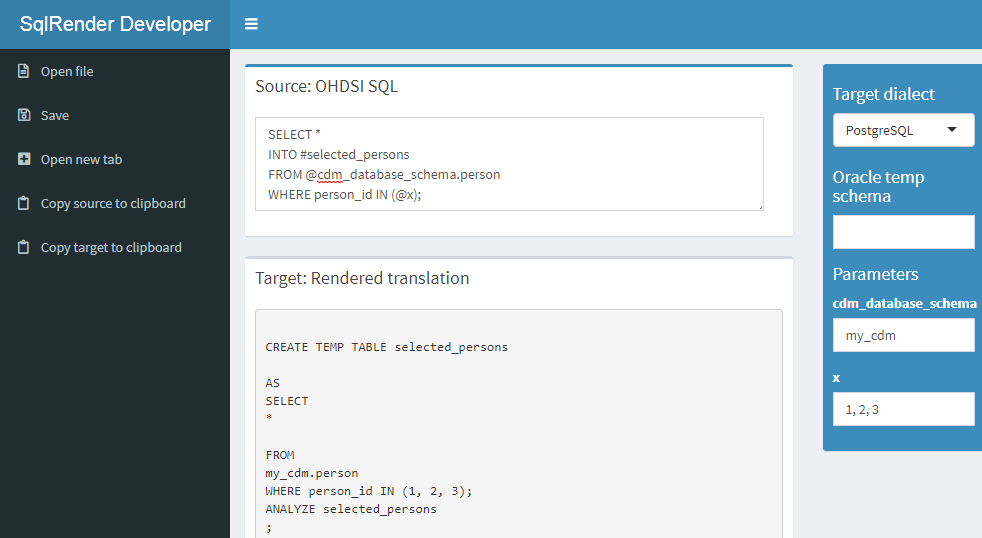
\includegraphics[width=1\linewidth]{images/SqlAndR/sqlDeveloper} 

}

\caption{The SqlDeveloper Shiny app.}\label{fig:sqlDeveloper}
\end{figure}

このアプリでは、OHDSI SQLを入力し、ターゲットの方言を選択し、SQLに表示されるパラメータの値を入力すると、翻訳が自動的に下部に表示されます。

\section{DatabaseConnector}\label{DatabaseConnector}

\href{https://ohdsi.github.io/DatabaseConnector/}{DatabaseConnector}は、JavaのJDBCドライバを使用してさまざまなデータベースプラットフォームに接続するためのRパッケージです。DatabaseConnectorパッケージはCRAN(Comprehensive R Archive Network)で入手可能で、次のようにインストールできます:

\begin{Shaded}
\begin{Highlighting}[]
\FunctionTok{install.packages}\NormalTok{(}\StringTok{"DatabaseConnector"}\NormalTok{)}
\end{Highlighting}
\end{Shaded}

DatabaseConnectorは、従来のデータベースシステム(PostgreSQL、Microsoft SQL Server、SQLite、およびOracle)、並列データウェアハウス(Microsoft APS、IBM Netezza、Amazon)、ならびにビッグデータプラットフォーム(Hadoopを介したImpala、およびGoogle BigQuery)など、広範な技術プラットフォームをサポートしています。このパッケージにはすでにほとんどのドライバが含まれていますが、ライセンス上の理由からBigQuery、Netezza、Impalaのドライバは含まれておらず、ユーザーが入手する必要があります。これらのドライバのダウンロード方法については、\texttt{?jdbcDrivers}を参照ください。ダウンロード後、\texttt{connect}、\texttt{dbConnect}、\texttt{createConnectionDetails}関数の\texttt{pathToDriver}引数を使用できます。

\subsection{接続の作成}\label{ux63a5ux7d9aux306eux4f5cux6210}

データベースに接続するには、データベースプラットフォーム、サーバーの位置、ユーザー名、パスワードなど、多くの詳細を指定する必要があります。\texttt{connect}関数を呼び出し、これらの詳細を直接指定することができます: \index{DatabaseConnector!creating a connection}

\begin{Shaded}
\begin{Highlighting}[]
\NormalTok{conn }\OtherTok{\textless{}{-}} \FunctionTok{connect}\NormalTok{(}\AttributeTok{dbms =} \StringTok{"postgresql"}\NormalTok{,}
                \AttributeTok{server =} \StringTok{"localhost/postgres"}\NormalTok{,}
                \AttributeTok{user =} \StringTok{"joe"}\NormalTok{,}
                \AttributeTok{password =} \StringTok{"secret"}\NormalTok{,}
                \AttributeTok{schema =} \StringTok{"cdm"}\NormalTok{)}
\end{Highlighting}
\end{Shaded}

\begin{verbatim}
## Connecting using PostgreSQL driver
\end{verbatim}

各プラットフォームに必要な詳細情報については、\texttt{?connect}を参照ください。接続を閉じたことを必ず確認ください:

\begin{Shaded}
\begin{Highlighting}[]
\FunctionTok{disconnect}\NormalTok{(conn)}
\end{Highlighting}
\end{Shaded}

サーバー名を指定する代わりに、JDBC接続文字列を提供することも可能です。さらに便利な場合は、こちらを使用することもできます。:

\begin{Shaded}
\begin{Highlighting}[]
\NormalTok{connString }\OtherTok{\textless{}{-}} \StringTok{"jdbc:postgresql://localhost:5432/postgres"}
\NormalTok{conn }\OtherTok{\textless{}{-}} \FunctionTok{connect}\NormalTok{(}\AttributeTok{dbms =} \StringTok{"postgresql"}\NormalTok{,}
                \AttributeTok{connectionString =}\NormalTok{ connString,}
                \AttributeTok{user =} \StringTok{"joe"}\NormalTok{,}
                \AttributeTok{password =} \StringTok{"secret"}\NormalTok{,}
                \AttributeTok{schema =} \StringTok{"cdm"}\NormalTok{)}
\end{Highlighting}
\end{Shaded}

\begin{verbatim}
## Connecting using PostgreSQL driver
\end{verbatim}

場合によっては、接続の詳細を先に指定し、接続を後にしたい場合もあるでしょう。例えば、接続が関数内で確立される場合、詳細を引数として渡す必要がある場合に有用です。この目的には、\texttt{createConnectionDetails}関数を使用できます:

\begin{Shaded}
\begin{Highlighting}[]
\NormalTok{details }\OtherTok{\textless{}{-}} \FunctionTok{createConnectionDetails}\NormalTok{(}\AttributeTok{dbms =} \StringTok{"postgresql"}\NormalTok{,}
                                   \AttributeTok{server =} \StringTok{"localhost/postgres"}\NormalTok{,}
                                   \AttributeTok{user =} \StringTok{"joe"}\NormalTok{,}
                                   \AttributeTok{password =} \StringTok{"secret"}\NormalTok{,}
                                   \AttributeTok{schema =} \StringTok{"cdm"}\NormalTok{)}
\NormalTok{conn }\OtherTok{\textless{}{-}} \FunctionTok{connect}\NormalTok{(details)}
\end{Highlighting}
\end{Shaded}

\begin{verbatim}
## Connecting using PostgreSQL driver
\end{verbatim}

\subsection{クエリの実行}\label{ux30afux30a8ux30eaux306eux5b9fux884c}

データベースにクエリを実行するための主な関数は、\texttt{querySql}と\texttt{executeSql}です。\texttt{querySql}はデータがデータベースから返されることを想定しており、一度に1つのSQL文のみを処理できます。一方、\texttt{executeSql}はデータが返されることを想定せず、複数のSQL文を1つのSQL文字列で受け入れます。 \index{DatabaseConnector!querying}

いくつかの例を挙げます:

\begin{Shaded}
\begin{Highlighting}[]
\FunctionTok{querySql}\NormalTok{(conn, }\StringTok{"SELECT TOP 3 * FROM person"}\NormalTok{)}
\end{Highlighting}
\end{Shaded}

\begin{verbatim}
##   person_id gender_concept_id year_of_birth
## 1         1              8507          1975
## 2         2              8507          1976
## 3         3              8507          1977
\end{verbatim}

\begin{Shaded}
\begin{Highlighting}[]
\FunctionTok{executeSql}\NormalTok{(conn, }\StringTok{"TRUNCATE TABLE foo; DROP TABLE foo;"}\NormalTok{)}
\end{Highlighting}
\end{Shaded}

どちらの関数も広範なエラーレポートを提供します:サーバーによってエラーが発生した場合、エラーメッセージと問題のあるSQL文がテキストファイルに書き込まれ、デバッグが容易になります。また、\texttt{executeSql}関数はデフォルトで進行状況バーを表示し、実行されたSQL文の割合を示します。それらの属性が不要な場合は、\texttt{lowLevelQuerySql}と\texttt{lowLevelExecuteSql}関数がパッケージに用意されています。

\subsection{ffdfオブジェクトを使用したクエリの実行}\label{ffdfux30aaux30d6ux30b8ux30a7ux30afux30c8ux3092ux4f7fux7528ux3057ux305fux30afux30a8ux30eaux306eux5b9fux884c}

データベースから取得するデータがメモリに収まりきらないほど大きい場合もあります。セクション\ref{BigDataSupport} で述べたように、そのような場合には\texttt{ff}パッケージを使用してRデータオブジェクトをファイルに保存し、メモリ上にあるかのように使用することができます。\texttt{DatabaseConnector}はデータを直接ffdfオブジェクトにダウンロードすることができます:

\begin{Shaded}
\begin{Highlighting}[]
\NormalTok{x }\OtherTok{\textless{}{-}} \FunctionTok{querySql.ffdf}\NormalTok{(conn, }\StringTok{"SELECT * FROM person"}\NormalTok{)}
\end{Highlighting}
\end{Shaded}

xは現在ffdfオブジェクトです。

\subsection{同じSQLを用いて異なるプラットフォームにクエリを実行する}\label{ux540cux3058sqlux3092ux7528ux3044ux3066ux7570ux306aux308bux30d7ux30e9ux30c3ux30c8ux30d5ux30a9ux30fcux30e0ux306bux30afux30a8ux30eaux3092ux5b9fux884cux3059ux308b}

SqlRenderパッケージの\texttt{render}と\texttt{translate}関数を最初に呼び出す便利な関数があります:\texttt{renderTranslateExecuteSql}、\texttt{renderTranslateQuerySql}、\texttt{renderTranslateQuerySql.ffdf}。例えば:

\begin{Shaded}
\begin{Highlighting}[]
\NormalTok{x }\OtherTok{\textless{}{-}} \FunctionTok{renderTranslateQuerySql}\NormalTok{(conn,}
                             \AttributeTok{sql =} \StringTok{"SELECT TOP 10 * FROM @schema.person"}\NormalTok{,}
                             \AttributeTok{schema =} \StringTok{"cdm\_synpuf"}\NormalTok{)}
\end{Highlighting}
\end{Shaded}

SQL Server固有の「TOP 10」構文は、PostgreSQLでは「LIMIT 10」などに変換され、SQLパラメーター\texttt{@schema}は提供された値「cdm\_synpuf」に置き換えられます。

\subsection{テーブルの挿入}\label{ux30c6ux30fcux30d6ux30ebux306eux633fux5165}

データをデータベースに挿入するには\texttt{executeSql}関数を使用してSQLステートメントを送信することも可能ですが、最適化により\texttt{insertTable}関数を使用する方がより便利で高速です:

\begin{Shaded}
\begin{Highlighting}[]
\FunctionTok{data}\NormalTok{(mtcars)}
\FunctionTok{insertTable}\NormalTok{(conn, }\StringTok{"mtcars"}\NormalTok{, mtcars, }\AttributeTok{createTable =} \ConstantTok{TRUE}\NormalTok{)}
\end{Highlighting}
\end{Shaded}

この例では、mtcarsデータフレームをサーバー上の「mtcars」というテーブルにアップロードします。このテーブルは自動的に作成されます。

\section{CDMへのクエリ}\label{QueryTheCdm}

以下の例では、OHDSI SQLを使用してCDMに準拠したデータベースにクエリを実行します。これらのクエリでは、CDMのデータベーススキーマを示すために\texttt{@cdm}を使用します。

まず、データベースに何人の人がいるかをクエリで取得してみましょう:

\begin{Shaded}
\begin{Highlighting}[]
\KeywordTok{SELECT} \FunctionTok{COUNT}\NormalTok{(}\OperatorTok{*}\NormalTok{) }\KeywordTok{AS}\NormalTok{ person\_count }\KeywordTok{FROM}\NormalTok{ @cdm.person;}
\end{Highlighting}
\end{Shaded}

\begin{longtable}[]{@{}r@{}}
\toprule\noalign{}
PERSON\_COUNT \\
\midrule\noalign{}
\endhead
\bottomrule\noalign{}
\endlastfoot
26299001 \\
\end{longtable}

あるいは、観察期間の平均的な長なさに興味があるのかもしれません:

\begin{Shaded}
\begin{Highlighting}[]
\KeywordTok{SELECT} \FunctionTok{AVG}\NormalTok{(DATEDIFF(}\DataTypeTok{DAY}\NormalTok{,}
\NormalTok{                    observation\_period\_start\_date,}
\NormalTok{                    observation\_period\_end\_date) }\OperatorTok{/} \FloatTok{365.25}\NormalTok{) }\KeywordTok{AS}\NormalTok{ num\_years}
\KeywordTok{FROM}\NormalTok{ @cdm.observation\_period;}
\end{Highlighting}
\end{Shaded}

\begin{longtable}[]{@{}r@{}}
\toprule\noalign{}
NUM\_YEARS \\
\midrule\noalign{}
\endhead
\bottomrule\noalign{}
\endlastfoot
1.980803 \\
\end{longtable}

テーブルを結合して追加の統計を生成することができます。結合は通常、テーブル内の特定のフィールドに同じ値があることを要求することによって、複数のテーブルのフィールドを結合します。例えば、ここでは、両方のテーブルのPERSON\_IDフィールドで、PERSONテーブルとOBSERVATION\_PERIODテーブルを結合しています。つまり、結合の結果は、2つのテーブルのすべてのフィールドを持つ新しいテーブルのようなセットですが、すべての行において、2つのテーブルのPERSON\_IDフィールドは同じ値でなければなりません。例えば、OBSERVATION\_PERIODテーブルのOBSERVATION\_PERIOD\_END\_DATEフィールドと、PERSONテーブルのyear\_of\_birthフィールドを組み合わせて使用することで、観察終了時の最大年齢を計算することができます。:

\begin{Shaded}
\begin{Highlighting}[]
\KeywordTok{SELECT} \FunctionTok{MAX}\NormalTok{(}\DataTypeTok{YEAR}\NormalTok{(observation\_period\_end\_date) }\OperatorTok{{-}}
\NormalTok{           year\_of\_birth) }\KeywordTok{AS}\NormalTok{ max\_age}
\KeywordTok{FROM}\NormalTok{ @cdm.person}
\KeywordTok{INNER} \KeywordTok{JOIN}\NormalTok{ @cdm.observation\_period}
  \KeywordTok{ON}\NormalTok{ person.person\_id }\OperatorTok{=}\NormalTok{ observation\_period.person\_id;}
\end{Highlighting}
\end{Shaded}

\begin{longtable}[]{@{}r@{}}
\toprule\noalign{}
MAX\_AGE \\
\midrule\noalign{}
\endhead
\bottomrule\noalign{}
\endlastfoot
90 \\
\end{longtable}

観察開始時の年齢分布を決定するには、はるかに複雑なクエリが必要です。このクエリでは、まずPERSONをOBSERVATION\_PERIODテーブルに結合して観察開始時の年齢を計算します。また、この結合されたセットの順序を年齢に基づいて計算し、それをorder\_nrとして保存します。この結合の結果を複数回使用したい場合には、共通テーブル式(CTE)として定義し(\texttt{WITH\ ...\ AS}を使用)、``ages''と呼びます。これにより、agesを既存のテーブルであるかのように参照することができます。agesの行数を数えて''n''を生成し、各分位数に対して、order\_nrが分数のn倍より小さい最小年齢を求めます。例えば、中央値を求めるには\$\texttt{order\_nr\ \textless{}\ .50\ *\ n}の最小年齢を使用します。最小年齢と最大年齢は別々に計算されます:

\begin{Shaded}
\begin{Highlighting}[]
\KeywordTok{WITH}\NormalTok{ ages}
\KeywordTok{AS}\NormalTok{ (}
    \KeywordTok{SELECT}\NormalTok{ age,}
        \FunctionTok{ROW\_NUMBER}\NormalTok{() }\KeywordTok{OVER}\NormalTok{ (}
            \KeywordTok{ORDER} \KeywordTok{BY}\NormalTok{ age}
\NormalTok{            ) order\_nr}
    \KeywordTok{FROM}\NormalTok{ (}
        \KeywordTok{SELECT} \DataTypeTok{YEAR}\NormalTok{(observation\_period\_start\_date) }\OperatorTok{{-}}\NormalTok{ year\_of\_birth }\KeywordTok{AS}\NormalTok{ age}
        \KeywordTok{FROM}\NormalTok{ @cdm.person}
        \KeywordTok{INNER} \KeywordTok{JOIN}\NormalTok{ @cdm.observation\_period}
            \KeywordTok{ON}\NormalTok{ person.person\_id }\OperatorTok{=}\NormalTok{ observation\_period.person\_id}
\NormalTok{        ) age\_computed}
\NormalTok{    )}
\KeywordTok{SELECT} \FunctionTok{MIN}\NormalTok{(age) }\KeywordTok{AS}\NormalTok{ min\_age,}
    \FunctionTok{MIN}\NormalTok{(}\ControlFlowTok{CASE}
            \ControlFlowTok{WHEN}\NormalTok{ order\_nr }\OperatorTok{\textless{}}\NormalTok{ .}\DecValTok{25} \OperatorTok{*}\NormalTok{ n}
                \ControlFlowTok{THEN} \DecValTok{9999}
            \ControlFlowTok{ELSE}\NormalTok{ age}
            \ControlFlowTok{END}\NormalTok{) }\KeywordTok{AS}\NormalTok{ q25\_age,}
    \FunctionTok{MIN}\NormalTok{(}\ControlFlowTok{CASE}
            \ControlFlowTok{WHEN}\NormalTok{ order\_nr }\OperatorTok{\textless{}}\NormalTok{ .}\DecValTok{50} \OperatorTok{*}\NormalTok{ n}
                \ControlFlowTok{THEN} \DecValTok{9999}
            \ControlFlowTok{ELSE}\NormalTok{ age}
            \ControlFlowTok{END}\NormalTok{) }\KeywordTok{AS}\NormalTok{ median\_age,}
    \FunctionTok{MIN}\NormalTok{(}\ControlFlowTok{CASE}
            \ControlFlowTok{WHEN}\NormalTok{ order\_nr }\OperatorTok{\textless{}}\NormalTok{ .}\DecValTok{75} \OperatorTok{*}\NormalTok{ n}
                \ControlFlowTok{THEN} \DecValTok{9999}
            \ControlFlowTok{ELSE}\NormalTok{ age}
            \ControlFlowTok{END}\NormalTok{) }\KeywordTok{AS}\NormalTok{ q75\_age,}
    \FunctionTok{MAX}\NormalTok{(age) }\KeywordTok{AS}\NormalTok{ max\_age}
\KeywordTok{FROM}\NormalTok{ ages}
\KeywordTok{CROSS} \KeywordTok{JOIN}\NormalTok{ (}
    \KeywordTok{SELECT} \FunctionTok{COUNT}\NormalTok{(}\OperatorTok{*}\NormalTok{) }\KeywordTok{AS}\NormalTok{ n}
    \KeywordTok{FROM}\NormalTok{ ages}
\NormalTok{    ) population\_size;}
\end{Highlighting}
\end{Shaded}

\begin{longtable}[]{@{}rrrrr@{}}
\toprule\noalign{}
MIN\_AGE & Q25\_AGE & MEDIAN\_AGE & Q75\_AGE & MAX\_AGE \\
\midrule\noalign{}
\endhead
\bottomrule\noalign{}
\endlastfoot
0 & 6 & 17 & 34 & 90 \\
\end{longtable}

より複雑な計算は、SQLの代わりにRを使用して行うこともできます。例えば、同じ結果を得るため、次のRコードを使用することができます:

\begin{Shaded}
\begin{Highlighting}[]
\NormalTok{sql }\OtherTok{\textless{}{-}} \StringTok{"SELECT YEAR(observation\_period\_start\_date) {-}}
\StringTok{               year\_of\_birth AS age}
\StringTok{FROM @cdm.person}
\StringTok{INNER JOIN @cdm.observation\_period}
\StringTok{  ON person.person\_id = observation\_period.person\_id;"}
\NormalTok{age }\OtherTok{\textless{}{-}} \FunctionTok{renderTranslateQuerySql}\NormalTok{(conn, sql, }\AttributeTok{cdm =} \StringTok{"cdm"}\NormalTok{)}
\FunctionTok{quantile}\NormalTok{(age[, }\DecValTok{1}\NormalTok{], }\FunctionTok{c}\NormalTok{(}\DecValTok{0}\NormalTok{, }\FloatTok{0.25}\NormalTok{, }\FloatTok{0.5}\NormalTok{, }\FloatTok{0.75}\NormalTok{, }\DecValTok{1}\NormalTok{))}
\end{Highlighting}
\end{Shaded}

\begin{verbatim}
##   0%  25%  50%  75% 100%
##    0    6   17   34   90
\end{verbatim}

ここでは、サーバー上で年齢を計算し、すべての年齢をダウンロードし、年齢分布を計算します。しかし、これにはデータベースサーバーから数百万行ものデータをダウンロードする必要があり、効率的ではありません。計算をSQLで行うかRで行うかは、ケースバイケースで判断する必要があります。

クエリでは、CDM内のソース値を使用することができます。例えば、最も頻度の高いコンディションのソースコードのトップ10を取得するには、以下を用います:

\begin{Shaded}
\begin{Highlighting}[]
\KeywordTok{SELECT}\NormalTok{ TOP }\DecValTok{10}\NormalTok{ condition\_source\_value,}
  \FunctionTok{COUNT}\NormalTok{(}\OperatorTok{*}\NormalTok{) }\KeywordTok{AS}\NormalTok{ code\_count}
\KeywordTok{FROM}\NormalTok{ @cdm.condition\_occurrence}
\KeywordTok{GROUP} \KeywordTok{BY}\NormalTok{ condition\_source\_value}
\KeywordTok{ORDER} \KeywordTok{BY} \OperatorTok{{-}}\FunctionTok{COUNT}\NormalTok{(}\OperatorTok{*}\NormalTok{);}
\end{Highlighting}
\end{Shaded}

\begin{longtable}[]{@{}rr@{}}
\toprule\noalign{}
CONDITION\_SOURCE\_VALUE & CODE\_COUNT \\
\midrule\noalign{}
\endhead
\bottomrule\noalign{}
\endlastfoot
4019 & 49094668 \\
25000 & 36149139 \\
78099 & 28908399 \\
319 & 25798284 \\
31401 & 22547122 \\
317 & 22453999 \\
311 & 19626574 \\
496 & 19570098 \\
I10 & 19453451 \\
3180 & 18973883 \\
\end{longtable}

ここでは、CONDITION\_OCCURRENCEテーブル内のCONDITION\_SOURCE\_VALUEフィールドの値でレコードをグループ化し、各グループのレコード数をカウントしました。CONDITION\_SOURCE\_VALUEとそのカウントを取得し、カウントで逆順で並べ替えています。

\section{クエリ実行時にボキャブラリを使用する}\label{ux30afux30a8ux30eaux5b9fux884cux6642ux306bux30dcux30adux30e3ux30d6ux30e9ux30eaux3092ux4f7fux7528ux3059ux308b}

多くの操作では、ボキャブラリが有用です。ボキャブラリテーブルはCDMの一部であり、SQLクエリを使用して利用できます。ここでは、ボキャブラリに対するクエリをCDMに対するクエリと組み合わせる方法を示します。CDMの多くのフィールドにはコンセプトIDが含まれていますが、これらはCONCEPTテーブルを使用して解決できます。例えば、データベース内の人数を性別で階層化してカウントしたい場合、GENDER\_CONCEPT\_IDフィールドをコンセプト名に解決すると便利です:

\begin{Shaded}
\begin{Highlighting}[]
\KeywordTok{SELECT} \FunctionTok{COUNT}\NormalTok{(}\OperatorTok{*}\NormalTok{) }\KeywordTok{AS}\NormalTok{ subject\_count,}
\NormalTok{  concept\_name}
\KeywordTok{FROM}\NormalTok{ @cdm.person}
\KeywordTok{INNER} \KeywordTok{JOIN}\NormalTok{ @cdm.concept}
  \KeywordTok{ON}\NormalTok{ person.gender\_concept\_id }\OperatorTok{=}\NormalTok{ concept.concept\_id}
\KeywordTok{GROUP} \KeywordTok{BY}\NormalTok{ concept\_name;}
\end{Highlighting}
\end{Shaded}

\begin{longtable}[]{@{}rr@{}}
\toprule\noalign{}
SUBJECT\_COUNT & CONCEPT\_NAME \\
\midrule\noalign{}
\endhead
\bottomrule\noalign{}
\endlastfoot
14927548 & FEMALE \\
11371453 & MALE \\
\end{longtable}

ボキャブラリの非常に強力な機能の一つは、その階層構造です。よくあるクエリは、特定のコンセプトと \emph{そのすべての子孫}を探すものです。例えば、イププロフェンという成分を含む処方件数を数えるとします:

\begin{Shaded}
\begin{Highlighting}[]
\KeywordTok{SELECT} \FunctionTok{COUNT}\NormalTok{(}\OperatorTok{*}\NormalTok{) }\KeywordTok{AS}\NormalTok{ prescription\_count}
\KeywordTok{FROM}\NormalTok{ @cdm.drug\_exposure}
\KeywordTok{INNER} \KeywordTok{JOIN}\NormalTok{ @cdm.concept\_ancestor}
  \KeywordTok{ON}\NormalTok{ drug\_concept\_id }\OperatorTok{=}\NormalTok{ descendant\_concept\_id}
\KeywordTok{INNER} \KeywordTok{JOIN}\NormalTok{ @cdm.concept ingredient}
  \KeywordTok{ON}\NormalTok{ ancestor\_concept\_id }\OperatorTok{=}\NormalTok{ ingredient.concept\_id}
\KeywordTok{WHERE} \FunctionTok{LOWER}\NormalTok{(ingredient.concept\_name) }\OperatorTok{=} \StringTok{\textquotesingle{}ibuprofen\textquotesingle{}}
  \KeywordTok{AND}\NormalTok{ ingredient.concept\_class\_id }\OperatorTok{=} \StringTok{\textquotesingle{}Ingredient\textquotesingle{}}
  \KeywordTok{AND}\NormalTok{ ingredient.standard\_concept }\OperatorTok{=} \StringTok{\textquotesingle{}S\textquotesingle{}}\NormalTok{;}
\end{Highlighting}
\end{Shaded}

\begin{longtable}[]{@{}r@{}}
\toprule\noalign{}
PRESCRIPTION\_COUNT \\
\midrule\noalign{}
\endhead
\bottomrule\noalign{}
\endlastfoot
26871214 \\
\end{longtable}

\section{QueryLibrary}\label{querylibrary}

\index{QueryLibrary}

QueryLibraryは、CDM用の一般に使用されるSQLクエリのライブラリです。これはオンラインアプリケーション\footnote{\url{http://data.ohdsi.org/QueryLibrary}}として提供されており、図\ref{fig:queryLibrary}に示すように、Rパッケージとしても利用できます\footnote{\url{https://github.com/OHDSI/QueryLibrary}}。

\begin{figure}

{\centering 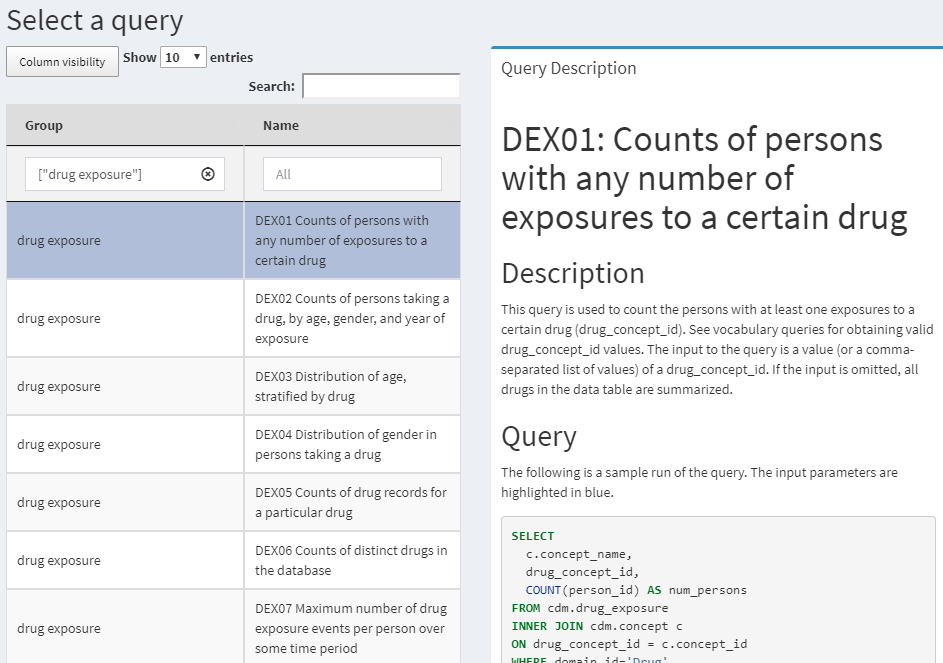
\includegraphics[width=1\linewidth]{images/SqlAndR/queryLibrary} 

}

\caption{クエリライブラリ:CDMに対するSQLクエリのライブラリ。}\label{fig:queryLibrary}
\end{figure}

このライブラリの目的は、新しいユーザーがCDMのクエリ方法を学習するのを支援することです。ライブラリ内のクエリは、OHDSIコミュニティによって審査され、承認されています。クエリライブラリは主にトレーニング目的で使用されますが、経験豊富なユーザーにとっても貴重なリソースとなります。

QueryLibraryは、SqlRenderを利用して、選択したSQL方言でクエリを実行します。ユーザーはCDMのデータベーススキーマ、ボキャブラリデータベーススキーマ(別々のものがある場合)、Oracleテンポラリスキーマ(必要な場合)を指定することもでき、これらの設定でクエリが自動的にレンダリングされます。

\section{簡単な研究のデザイン}\label{ux7c21ux5358ux306aux7814ux7a76ux306eux30c7ux30b6ux30a4ux30f3}

\subsection{問題の定義}\label{ux554fux984cux306eux5b9aux7fa9}

血管性浮腫は、ACE阻害薬(ACEi)のよく知られた副作用です。\citet{slater_1988} によると、ACEi治療開始後1週間の血管性浮腫の発症率は3,000人中1例/週と推定されています。ここでは、この結果を再現し、年齢と性別によって層別化します。単純化するため、ACEiの一つである(リシノプリル)に焦点を当てます。したがって、次の問いに答えます:

\begin{quote}
リシノプリル投与開始後の最初の1週間での血管性浮腫の発生率は、年齢と性別で層別化するとどの程度でしょうか?
\end{quote}

\subsection{曝露}\label{ux66ddux9732}

曝露をリシノプリルへの初回の曝露として定義します。初回とは、以前にリシノプリルへの曝露がないことを意味します。初回の曝露の前に365日間の連続した観察期間が必要となります。

\subsection{アウトカム}\label{ux30a2ux30a6ux30c8ux30abux30e0}

血管性浮腫は、入院中または救急外来(ER)受診中に血管性浮腫の診断コードが記録された場合と定義します。

\subsection{リスク期間}\label{ux30eaux30b9ux30afux671fux9593}

治療開始後の最初の1週間の発症率を計算します。患者が1週間にわたって継続的に曝露されたかどうかは問いません。

\section{SQLとRを使用した研究の実施}\label{sqlux3068rux3092ux4f7fux7528ux3057ux305fux7814ux7a76ux306eux5b9fux65bd}

OHDSIツールの慣例に縛られることはありませんが、同じ原則に従うことは有益です。この場合、OHDSIツールが動作するのと同様に、SQLを用いてコホートテーブルを作成します。COHORTテーブルはCDMに定義されており、使用する事前定義されたフィールドセットもあります。まず、書き込み権限のあるデータベーススキーマにCOHORTテーブルを作成する必要がありますが、これはCDM形式でデータを保持しているスキーマとは異なるスキーマである可能性が高いです。

\begin{Shaded}
\begin{Highlighting}[]
\FunctionTok{library}\NormalTok{(DatabaseConnector)}
\NormalTok{conn }\OtherTok{\textless{}{-}} \FunctionTok{connect}\NormalTok{(}\AttributeTok{dbms =} \StringTok{"postgresql"}\NormalTok{,}
                \AttributeTok{server =} \StringTok{"localhost/postgres"}\NormalTok{,}
                \AttributeTok{user =} \StringTok{"joe"}\NormalTok{,}
                \AttributeTok{password =} \StringTok{"secret"}\NormalTok{)}
\NormalTok{cdmDbSchema }\OtherTok{\textless{}{-}} \StringTok{"cdm"}
\NormalTok{cohortDbSchema }\OtherTok{\textless{}{-}} \StringTok{"scratch"}
\NormalTok{cohortTable }\OtherTok{\textless{}{-}} \StringTok{"my\_cohorts"}

\NormalTok{sql }\OtherTok{\textless{}{-}} \StringTok{"}
\StringTok{CREATE TABLE @cohort\_db\_schema.@cohort\_table (}
\StringTok{  cohort\_definition\_id INT,}
\StringTok{  cohort\_start\_date DATE,}
\StringTok{  cohort\_end\_date DATE,}
\StringTok{  subject\_id BIGINT}
\StringTok{);}
\StringTok{"}
\FunctionTok{renderTranslateExecuteSql}\NormalTok{(conn, sql,}
                          \AttributeTok{cohort\_db\_schema =}\NormalTok{ cohortDbSchema,}
                          \AttributeTok{cohort\_table =}\NormalTok{ cohortTable)}
\end{Highlighting}
\end{Shaded}

ここでは、データベーススキーマとテーブル名をパラメータ化しています。異なる環境に簡単に適応させることができます。その結果、データベースサーバー上に空のテーブルが作成されます。

\subsection{曝露コホート}\label{ux66ddux9732ux30b3ux30dbux30fcux30c8}

次に、曝露コホートを作成し、COHORTテーブルに挿入します:

\begin{Shaded}
\begin{Highlighting}[]
\NormalTok{sql }\OtherTok{\textless{}{-}} \StringTok{"}
\StringTok{INSERT INTO @cohort\_db\_schema.@cohort\_table (}
\StringTok{  cohort\_definition\_id,}
\StringTok{  cohort\_start\_date,}
\StringTok{  cohort\_end\_date,}
\StringTok{  subject\_id}
\StringTok{)}
\StringTok{SELECT 1 AS cohort\_definition\_id,}
\StringTok{  cohort\_start\_date,}
\StringTok{  cohort\_end\_date,}
\StringTok{  subject\_id}
\StringTok{FROM (}
\StringTok{  SELECT drug\_era\_start\_date AS cohort\_start\_date,}
\StringTok{    drug\_era\_end\_date AS cohort\_end\_date,}
\StringTok{    person\_id AS subject\_id}
\StringTok{  FROM (}
\StringTok{    SELECT drug\_era\_start\_date,}
\StringTok{      drug\_era\_end\_date,}
\StringTok{      person\_id,}
\StringTok{      ROW\_NUMBER() OVER (}
\StringTok{        PARTITION BY person\_id}
\StringTok{            ORDER BY drug\_era\_start\_date}
\StringTok{      ) order\_nr}
\StringTok{    FROM @cdm\_db\_schema.drug\_era}
\StringTok{    WHERE drug\_concept\_id = 1308216 {-}{-} リシノプリル}
\StringTok{  ) ordered\_exposures}
\StringTok{  WHERE order\_nr = 1}
\StringTok{) first\_era}
\StringTok{INNER JOIN @cdm\_db\_schema.observation\_period}
\StringTok{  ON subject\_id = person\_id}
\StringTok{    AND observation\_period\_start\_date \textless{} cohort\_start\_date}
\StringTok{    AND observation\_period\_end\_date \textgreater{} cohort\_start\_date}
\StringTok{WHERE DATEDIFF(DAY,}
\StringTok{               observation\_period\_start\_date,}
\StringTok{               cohort\_start\_date) \textgreater{}= 365;}
\StringTok{"}

\FunctionTok{renderTranslateExecuteSql}\NormalTok{(conn, sql,}
                          \AttributeTok{cohort\_db\_schema =}\NormalTok{ cohortDbSchema,}
                          \AttributeTok{cohort\_table =}\NormalTok{ cohortTable,}
                          \AttributeTok{cdm\_db\_schema =}\NormalTok{ cdmDbSchema)}
\end{Highlighting}
\end{Shaded}

ここでは、CDMの標準テーブルであるDRUG\_ERAテーブルを使用します。このテーブルはDRUG\_EXPOSUREテーブルから自動的に派生するものです。DRUG\_ERAテーブルには成分レベルでの継続的な曝露期間が含まれるため、リシノプリルを検索すると、自動的にリシノプリルを含む薬剤への曝露がすべて特定されます。次に、OBSERVATION\_PERIOD テーブルに結合し、1人当たりの最初の薬物曝露を取り出します。1人の患者が複数の観察期間を持つ可能性があるため、薬物曝露を含む期間のみに結合する必要があります。また、OBSERVATION\_PERIOD\_START\_DATE と COHORT\_START\_DATE の間には、少なくとも 365 日の間隔が必要となります。

\subsection{アウトカムコホート}\label{ux30a2ux30a6ux30c8ux30abux30e0ux30b3ux30dbux30fcux30c8}

最後に、アウトカムコホートを作成する必要があります:

\begin{Shaded}
\begin{Highlighting}[]
\NormalTok{sql }\OtherTok{\textless{}{-}} \StringTok{"}
\StringTok{INSERT INTO @cohort\_db\_schema.@cohort\_table (}
\StringTok{ cohort\_definition\_id,}
\StringTok{ cohort\_start\_date,}
\StringTok{ cohort\_end\_date,}
\StringTok{subject\_id}
\StringTok{)}
\StringTok{SELECT 2 AS cohort\_definition\_id,}
\StringTok{  cohort\_start\_date,}
\StringTok{  cohort\_end\_date,}
\StringTok{  subject\_id}
\StringTok{FROM (}
\StringTok{  SELECT DISTINCT person\_id AS subject\_id,}
\StringTok{    condition\_start\_date AS cohort\_start\_date,}
\StringTok{    condition\_end\_date AS cohort\_end\_date}
\StringTok{  FROM @cdm\_db\_schema.condition\_occurrence}
\StringTok{  INNER JOIN @cdm\_db\_schema.concept\_ancestor}
\StringTok{    ON condition\_concept\_id = descendant\_concept\_id}
\StringTok{  WHERE ancestor\_concept\_id = 432791 {-}{-} 血管浮腫}
\StringTok{) distinct\_occurrence}
\StringTok{INNER JOIN @cdm\_db\_schema.visit\_occurrence}
\StringTok{  ON subject\_id = person\_id}
\StringTok{  AND visit\_start\_date \textless{}= cohort\_start\_date}
\StringTok{  AND visit\_end\_date \textgreater{}= cohort\_start\_date}
\StringTok{WHERE visit\_concept\_id IN (262, 9203,}
\StringTok{    9201) {-}{-} 入院またはER;}
\StringTok{"}

\FunctionTok{renderTranslateExecuteSql}\NormalTok{(conn, sql,}
                          \AttributeTok{cohort\_db\_schema =}\NormalTok{ cohortDbSchema,}
                          \AttributeTok{cohort\_table =}\NormalTok{ cohortTable,}
                          \AttributeTok{cdm\_db\_schema =}\NormalTok{ cdmDbSchema)}
\end{Highlighting}
\end{Shaded}

ここでは、CONDITION\_OCCURRENCEテーブルをCONCEPT\_ANCESTORテーブルと結合して、血管性浮腫またはその下位層に含まれるすべての発生を見つけます。同じ日に複数の診断がある場合、それは同じ発生である可能性が高いため、各日1件のレコードのみを取得するようにDISTINCTを使用します。次に、診断が入院またはERで行われたことを確認するために、これらの発生をVISIT\_OCCURRENCEテーブルと結合します。

\subsection{発症率の計算}\label{ux767aux75c7ux7387ux306eux8a08ux7b97}

コホートが設定されたので、年齢と性別で層別化された発症率を計算できます:

\begin{Shaded}
\begin{Highlighting}[]
\NormalTok{sql }\OtherTok{\textless{}{-}} \StringTok{"}
\StringTok{WITH tar AS (}
\StringTok{  SELECT concept\_name AS gender,}
\StringTok{    FLOOR((YEAR(cohort\_start\_date) {-}}
\StringTok{          year\_of\_birth) / 10) AS age,}
\StringTok{    subject\_id,}
\StringTok{    cohort\_start\_date,}
\StringTok{    CASE WHEN DATEADD(DAY, 7, cohort\_start\_date) \textgreater{}}
\StringTok{      observation\_period\_end\_date}
\StringTok{    THEN observation\_period\_end\_date}
\StringTok{    ELSE DATEADD(DAY, 7, cohort\_start\_date)}
\StringTok{    END AS cohort\_end\_date}
\StringTok{  FROM @cohort\_db\_schema.@cohort\_table}
\StringTok{  INNER JOIN @cdm\_db\_schema.observation\_period}
\StringTok{    ON subject\_id = observation\_period.person\_id}
\StringTok{      AND observation\_period\_start\_date \textless{} cohort\_start\_date}
\StringTok{      AND observation\_period\_end\_date \textgreater{} cohort\_start\_date}
\StringTok{  INNER JOIN @cdm\_db\_schema.person}
\StringTok{    ON subject\_id = person.person\_id}
\StringTok{  INNER JOIN @cdm\_db\_schema.concept}
\StringTok{    ON gender\_concept\_id = concept\_id}
\StringTok{  WHERE cohort\_definition\_id = 1 {-}{-} 曝露}
\StringTok{)}
\StringTok{SELECT days.gender,}
\StringTok{    days.age,}
\StringTok{    days,}
\StringTok{    CASE WHEN events IS NULL THEN 0 ELSE events END AS events}
\StringTok{FROM (}
\StringTok{  SELECT gender,}
\StringTok{    age,}
\StringTok{    SUM(DATEDIFF(DAY, cohort\_start\_date,}
\StringTok{      cohort\_end\_date)) AS days}
\StringTok{  FROM tar}
\StringTok{  GROUP BY gender,}
\StringTok{    age}
\StringTok{) days}
\StringTok{LEFT JOIN (}
\StringTok{  SELECT gender,}
\StringTok{      age,}
\StringTok{      COUNT(*) AS events}
\StringTok{  FROM tar}
\StringTok{  INNER JOIN @cohort\_db\_schema.@cohort\_table angioedema}
\StringTok{    ON tar.subject\_id = angioedema.subject\_id}
\StringTok{      AND tar.cohort\_start\_date \textless{}= angioedema.cohort\_start\_date}
\StringTok{      AND tar.cohort\_end\_date \textgreater{}= angioedema.cohort\_start\_date}
\StringTok{  WHERE cohort\_definition\_id = 2 {-}{-} 結果}
\StringTok{  GROUP BY gender,}
\StringTok{    age}
\StringTok{) events}
\StringTok{ON days.gender = events.gender}
\StringTok{  AND days.age = events.age;}
\StringTok{"}

\NormalTok{results }\OtherTok{\textless{}{-}} \FunctionTok{renderTranslateQuerySql}\NormalTok{(conn, sql,}
                                   \AttributeTok{cohort\_db\_schema =}\NormalTok{ cohortDbSchema,}
                                   \AttributeTok{cohort\_table =}\NormalTok{ cohortTable,}
                                   \AttributeTok{cdm\_db\_schema =}\NormalTok{ cdmDbSchema,}
                                   \AttributeTok{snakeCaseToCamelCase =} \ConstantTok{TRUE}\NormalTok{)}
\end{Highlighting}
\end{Shaded}

まず、CTE「tar」を作成し、適切なリスク時間を伴うすべての曝露を含めます。OBSERVATION\_PERIOD\_END\_DATEでリスク期間が切り捨てられることに留意ください。また、10年ごとの年齢階層を計算し、性別を特定します。CTEを使用する利点は、クエリ中に同じ中間結果セットを複数回使用できることです。このユースケースでは、リスク期間の合計およびリスク期間中に発生する血管性浮腫のイベント数を数えるために使用します。

snakeCaseToCamelCase = TRUE を用いるのは、SQLではフィールド名にsnake\_case を使用する傾向がある(SQLは大文字と小文字を区別しないため)のに対し、RではcamelCaseを使用する傾向がある(Rは大文字・小文字を区別するため)からです。\texttt{results}データフレームの列名はcamelCaseになります。

ggplot2パッケージを使用すると、結果を簡単にプロットできます:

\begin{Shaded}
\begin{Highlighting}[]
\CommentTok{\# 発症率(IR)を算出}
\NormalTok{results}\SpecialCharTok{$}\NormalTok{ir }\OtherTok{\textless{}{-}} \DecValTok{1000} \SpecialCharTok{*}\NormalTok{ results}\SpecialCharTok{$}\NormalTok{events }\SpecialCharTok{/}\NormalTok{ results}\SpecialCharTok{$}\NormalTok{days }\SpecialCharTok{/} \DecValTok{7}

\CommentTok{\# 年齢スケールを修正}
\NormalTok{results}\SpecialCharTok{$}\NormalTok{age }\OtherTok{\textless{}{-}}\NormalTok{ results}\SpecialCharTok{$}\NormalTok{age }\SpecialCharTok{*} \DecValTok{10}

\FunctionTok{library}\NormalTok{(ggplot2)}
\FunctionTok{ggplot}\NormalTok{(results, }\FunctionTok{aes}\NormalTok{(}\AttributeTok{x =}\NormalTok{ age, }\AttributeTok{y =}\NormalTok{ ir, }\AttributeTok{group =}\NormalTok{ gender, }\AttributeTok{color =}\NormalTok{ gender)) }\SpecialCharTok{+}
  \FunctionTok{geom\_line}\NormalTok{() }\SpecialCharTok{+}
  \FunctionTok{xlab}\NormalTok{(}\StringTok{"年齢"}\NormalTok{) }\SpecialCharTok{+}
  \FunctionTok{ylab}\NormalTok{(}\StringTok{"発症率(1,000患者/週)"}\NormalTok{)}
\end{Highlighting}
\end{Shaded}

\begin{center}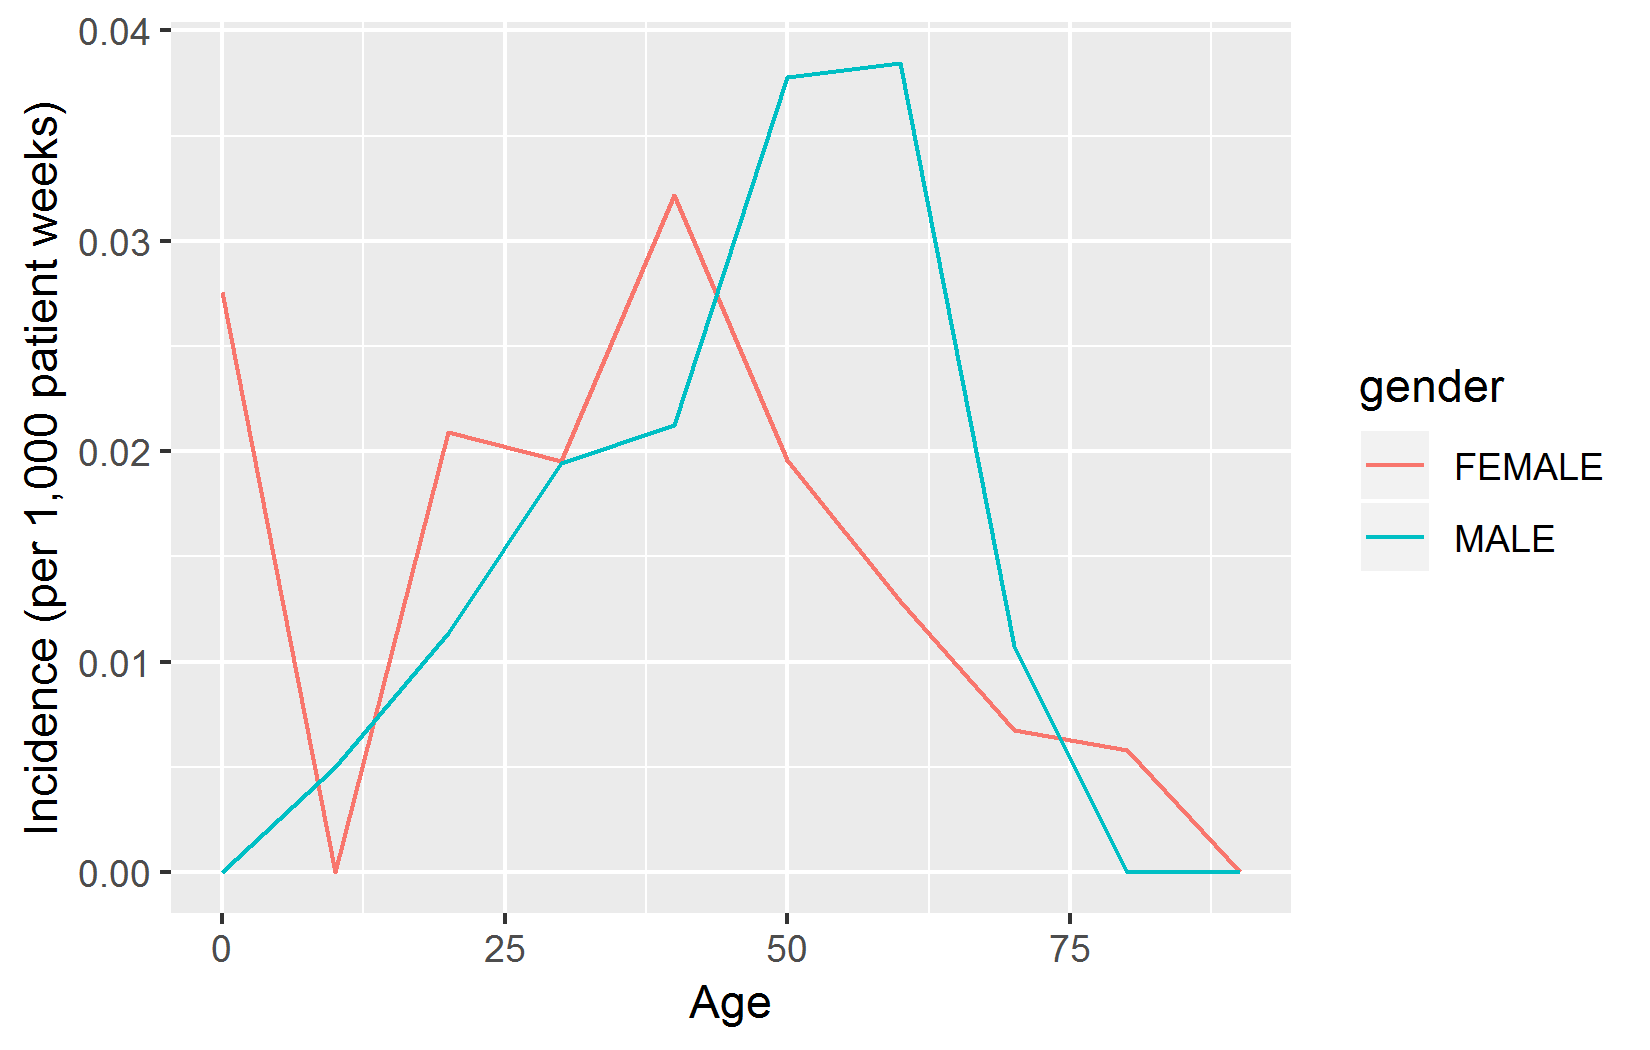
\includegraphics[width=0.8\linewidth]{images/SqlAndR/ir} \end{center}

\subsection{クリーンアップ}\label{ux30afux30eaux30fcux30f3ux30a2ux30c3ux30d7}

作成したテーブルをクリーンアップし、忘れずに接続を閉じます:

\begin{Shaded}
\begin{Highlighting}[]
\NormalTok{sql }\OtherTok{\textless{}{-}} \StringTok{"}
\StringTok{TRUNCATE TABLE @cohort\_db\_schema.@cohort\_table;}
\StringTok{DROP TABLE @cohort\_db\_schema.@cohort\_table;}
\StringTok{"}
\FunctionTok{renderTranslateExecuteSql}\NormalTok{(conn, sql,}
                          \AttributeTok{cohort\_db\_schema =}\NormalTok{ cohortDbSchema,}
                          \AttributeTok{cohort\_table =}\NormalTok{ cohortTable)}

\FunctionTok{disconnect}\NormalTok{(conn)}
\end{Highlighting}
\end{Shaded}

\subsection{互換性}\label{ux4e92ux63dbux6027}

OHDSI SQLとDatabaseConnectorとSqlRenderを組み合わせて使用するため、ここで紹介したコードはOHDSIがサポートする任意のデータベースプラットフォームで実行できます。

デモンストレーション用に、手作業でSQLを使用してコホートを作成することにしましたが、ATLASでコホート定義を構築し、ATLASで生成されたSQLを使用してコホートをインスタンス化する方が便利です。ATLASもOHDSI SQLを生成するため、SqlRenderとDatabaseConnectorと簡単に併用することができます。

\section{まとめ}\label{ux307eux3068ux3081-7}

\begin{rmdsummary}
\begin{itemize}
\item
  \textbf{SQL}(Structured Query Language)は、共通データモデル(CDM)に準拠したデータベースを含む、データベースに照会するための標準言語です。
\item
  異なるデータベースプラットフォームは異なるSQL表現を持っており、照会するためには異なるツールが必要です。
\item
  \textbf{SqlRender}と\textbf{DatabaseConnector}Rパッケージは、CDM内のデータを照会するための統一された方法を提供し、同じ分析コードを修正することなく異なる環境で実行できるようにします。
\item
  RとSQLを併用することで、OHDSIツールではサポートされていないカスタム分析を実装できます。
\item
  \textbf{QueryLibrary}は、CDM用の再利用可能なSQLクエリのコレクションを提供します。
\end{itemize}
\end{rmdsummary}

\section{演習}\label{ux6f14ux7fd2-4}

\subsubsection*{前提条件}\label{ux524dux63d0ux6761ux4ef6-3}
\addcontentsline{toc}{subsubsection}{前提条件}

これらの演習では、セクション \ref{installR} に記載されているように、R、R-Studio、Java がインストールされていることを前提とします。また、\href{https://ohdsi.github.io/SqlRender/}{SqlRender}、\href{https://ohdsi.github.io/DatabaseConnector/}{DatabaseConnector}、および \href{https://ohdsi.github.io/Eunomia/}{Eunomia} パッケージも必要です。以下の手順でインストールできます。

\begin{Shaded}
\begin{Highlighting}[]
\FunctionTok{install.packages}\NormalTok{(}\FunctionTok{c}\NormalTok{(}\StringTok{"SqlRender"}\NormalTok{, }\StringTok{"DatabaseConnector"}\NormalTok{, }\StringTok{"remotes"}\NormalTok{))}
\NormalTok{remotes}\SpecialCharTok{::}\FunctionTok{install\_github}\NormalTok{(}\StringTok{"ohdsi/Eunomia"}\NormalTok{, }\AttributeTok{ref =} \StringTok{"v1.0.0"}\NormalTok{)}
\end{Highlighting}
\end{Shaded}

Eunomia パッケージは、CDM 内でローカル R セッション内で動作するシミュレートされたデータセットを提供します。接続の詳細は以下の方法で取得できます。

\begin{Shaded}
\begin{Highlighting}[]
\NormalTok{connectionDetails }\OtherTok{\textless{}{-}}\NormalTok{ Eunomia}\SpecialCharTok{::}\FunctionTok{getEunomiaConnectionDetails}\NormalTok{()}
\end{Highlighting}
\end{Shaded}

CDM データベースのスキーマは「main」です。

\begin{exercise}
\protect\hypertarget{exr:exercisePeopleCount}{}\label{exr:exercisePeopleCount}SQL と R を使用して、データベース内に何人いるかを計算します。
\end{exercise}

\begin{exercise}
\protect\hypertarget{exr:exerciseCelecoxibUsers}{}\label{exr:exerciseCelecoxibUsers}SQL と R を使用して、セレコキシブの処方を少なくとも1回受けたことがある人の人数を計算します。
\end{exercise}

\begin{exercise}
\protect\hypertarget{exr:exerciseGiBleedsDuringCelecoxib}{}\label{exr:exerciseGiBleedsDuringCelecoxib}SQL と R を使用して、セレコキシブの服用中に消化管出血と診断された人の人数を計算します。(ヒント: 消化管出血のコンセプト ID は \href{http://athena.ohdsi.org/search-terms/terms/192671}{192671} です)
\end{exercise}

推奨される解答は付録 \ref{SqlAndRanswers} を参照ください。

\chapter{--翻訳作業中-- コホートの定義}\label{Cohorts}

\emph{章の著者: Kristin Kostka}

観察型健康データ(\emph{リアルワールドデータ}とも呼ばれる)は、患者の健康状態や医療の提供に関連するデータで、さまざまな情報源から日常的に収集されたデータです。そのため、OHDSIデータスチュワード(OHDSIの共同研究者で、各サイトのCDMにデータを維持している人々)は、電子健康記録(EHR)、医療保険請求データ、製品や疾患のレジストリ、自宅使用環境を含む患者が生成したデータ、およびモバイルデバイスなど健康状態に関する情報を提供できる他の情報源など、複数の情報源からデータをキャプチャする場合があります。これらのデータは研究目的で収集されたものではないため、興味のある臨床データ要素を明示的にキャプチャしていない場合があります。

たとえば、医療保険請求データベースは、あるコンディション(例:血管浮腫)に対して提供されたすべての医療をキャプチャして関連コストが適切に補償されるようにデザインされており、実際のコンディションに関する情報はこの目的の一環としてのみキャプチャされます。このような観察データを研究目的で使用したい場合、データにキャプチャされているものを使用して本当に興味のあるものを推測するためのロジックを作成する必要があります。つまり、臨床イベントがどのように現れるかの定義を使用してコホートを作成する必要があるのです。たとえば、保険請求データベースで血管浮腫イベントを特定したい場合、血管浮腫の診断コードが緊急室の設定で記録されていることを要求するロジックを定義し、過去の血管浮腫の発生に対するフォローアップケアを単に説明する請求から区別するかもしれません。類似の考慮事項は、EHRに記録された日常的な医療の相互作用でキャプチャされるデータに対しても適用されます。データが二次的な目的で使用されているため、各データベースが元々何を目的として設計されたかを認識する必要があります。研究をデザインするたびに、さまざまな医療環境でコホートがどのように存在するのかについての細かな点を考慮する必要があります。

この章では、コホート定義の作成と共有とは何か、コホートを開発する方法、およびATLASまたはSQLを使用して独自のコホートを作成する方法について説明します。

\section{コホートとは?}\label{ux30b3ux30dbux30fcux30c8ux3068ux306f}

OHDSI研究では、コホートを一つ以上の選択基準を満たし、一定期間にわたってこれを維持している人々の集合として定義します。この用語はしばしば\emph{表現型}と置き換えられます。コホートは、OHDSI分析ツールやネットワーク研究全体で研究質問を実行するための主要な構成要素として使用されます。たとえば、ACE阻害薬の開始による血管浮腫リスクを予測することを目的とした研究では、2つのコホートを定義します:アウトカムコホート(血管浮腫)およびターゲットコホート(ACE阻害薬を開始する人々)。OHDSIのコホートの重要な側面は、通常、研究内の他のコホートから独立して定義されるため、再利用が可能であることです。たとえば、血管浮腫コホートはターゲット集団外も含む集団全体のすべての血管浮腫イベントを特定します。分析時に必要に応じてこれらの二つのコホートの交差を取ります。この利点は、同じ血管浮腫コホート定義が、たとえばACE阻害薬と他の曝露を比較する推定研究など、他の分析でも使用できるということです。コホート定義は、研究の質問に応じて異なることがあります。

\begin{rmdimportant}
コホートは、一つ以上の選択基準を満たし、それを一定期間維持する人々の集合です。
\end{rmdimportant}

\index{コホート} \index{コホート定義} OHDSIで使用されるコホートの定義は、この分野の他の人々が使用するものとは異なるかもしれないことを理解することが重要です。たとえば、多くの査読済み科学論文では、コホートが特定の臨床コードのコードセット(例:ICD-9/ICD-10、NDC、HCPCSなど)に類似していると示唆されることがあります。コードセットはコホートを組み立てる際の重要な要素ですが、コホートはコードセットによって定義されません。コホートは、条件を満たすコードセットの使用方法に関する具体的なロジックを必要とします(例:これはICD-9/ICD-10コードの最初の発生ですか?任意の発生ですか?)。 よく定義されたコホートは、患者がコホートに入る方法とコホートから退出する方法を指定します。 \index{コードセット}

\index{表現型} OHDSIのコホート定義を利用するためのユニークなニュアンスには以下があります

\begin{itemize}
\tightlist
\item
  一人の人が複数のコホートに属する可能性があります
\item
  一人の人が同じコホートに異なる期間属する可能性があります
\item
  一人の人が同じ期間内に同じコホートに複数回属することはありません
\item
  コホートにはメンバーがゼロまたは複数いる場合があります
\end{itemize}

コホートを構築するための主要なアプローチは二つあります:

\begin{enumerate}
\def\labelenumi{\arabic{enumi}.}
\item
  \textbf{ルールベースのコホート定義} は、患者がコホートにいる時期を明示的なルールで説明します。これらのルールを定義するには通常、コホートの選択基準のルールを構築するために、対象となる治療領域の知識を持つ個人のドメインの専門知識に大きく依存する。
\item
  \textbf{確率的コホート定義} は、コホートにいる患者の確率(0から100\%の間の確率)を計算する確率モデルを使用します。この確率は、しきい値を使用してイエス・ノーの分類に変換できるか、または一部の研究デザインではそのまま使用できます。確率モデルは通常、機械学習(例:ロジスティック回帰)を使用して、関連する患者特性を自動的に特定するために例データでトレーニングされます。
\end{enumerate}

次のセクションでは、これらのアプローチについて詳しく説明します。

\section{ルールベースのコホート定義}\label{ux30ebux30fcux30ebux30d9ux30fcux30b9ux306eux30b3ux30dbux30fcux30c8ux5b9aux7fa9}

ルールベースのコホート定義は、特定の期間内に明示的に一つまたは、複数の選択基準(例:「血管浮腫のある人」)を定義することから始まります(例:「過去6ヶ月以内にこの状態を発症した人」)。\index{cohort!rule-based design}

これらの基準を組み立てるために使用する標準的なコンポーネントは次のとおりです:

\begin{itemize}
\item
  \textbf{ドメイン}:データが保存されているCDMドメイン(例:「処置の発生」、「薬剤曝露」)は、臨床情報の種類およびそのCDMテーブル内に表現可能なコンセプトを定義します。ドメインについては、セクション\ref{domains}で詳しく説明されています。
\item
  \textbf{コンセプトセット}:臨床実体を包含する一つ以上の標準コンセプトを定義するデータ非依存の表現です。これらのコンセプトセットは、異なる観察健康データ間で相互運用可能であり、ボキャブラリ内の標準用語にマッピングされる臨床実体を表します。コンセプトセットについては、セクション\ref{conceptSets}で詳しく説明されています。
\item
  \textbf{ドメイン固有の属性}:関心のある臨床実体に関連する追加の属性(例:DRUG\_EXPOSUREのDAYS\_SUPPLYやMEASUREMENTのVALUE\_AS\_NUMBERやRANGE\_HIGH)。
\item
  \textbf{時間ロジック}:選択基準とイベントとの関係を評価する時間間隔(例:指定された状態は曝露開始の365日前またはその日前後で発生する必要があります)。
\end{itemize}

コホート定義を構築する際、コホート属性を表すブロックのようにドメインを考えると便利です(図\ref{fig:cohortLegos}参照)。各ドメインの許容内容について混乱した場合は、共通データモデルの章(チャプター\ref{CommonDataModel})を参照してください。

\begin{figure}

{\centering 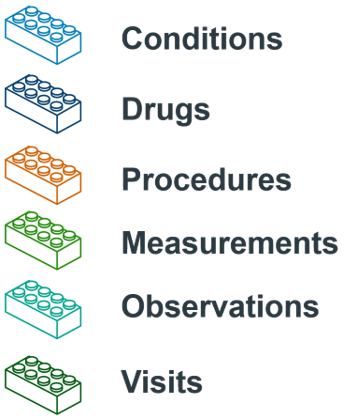
\includegraphics[width=0.5\linewidth]{images/Cohorts/cohort-legos} 

}

\caption{コホート定義のブロック}\label{fig:cohortLegos}
\end{figure}

コホート定義作成時に自問すべきいくつかの質問があります:

\begin{itemize}
\tightlist
\item
  \emph{コホートエントリの時間を定義する初期イベントは何か?}
\item
  \emph{初期イベントに適用される選択基準は何か?}
\item
  \emph{コホート退出の時間を定義するものは何か?}
\end{itemize}

\textbf{コホートエントリエベント}:コホートエントリエベント(初期イベント)は、人々がコホートに参加する時点、つまり\textbf{コホートインデックス日}を定義します。コホートエントリエベントは、薬剤曝露、コンディション、処置、測定値、受診期間など、CDMで記録された任意のイベントであり得ます。初期イベントは、データが保存されているCDMドメイン(例:PROCEDURE\_OCCURRENCE、DRUG\_EXPOSUREなど)、臨床活動を特定するために作成されたコンセプトセット(例:状態のためのSNOMEDコード、薬剤のためのRxNormコード)、およびその他の特定の属性(例:発生時の年齢、初診断/処置/その他、開始日と終了日の指定、受診期間または基準の指定、供給日数など)によって定義されます。エントリエベントを持つ人々のセットは\textbf{初期イベントコホート}と呼ばれます。\index{cohort!entry event}

\textbf{選択基準}:選択基準は、初期イベントコホートに適用され、さらに人々のセットを制限します。各選択基準は、データが保存されているCDMドメイン、臨床活動を表すコンセプトセット、ドメイン固有の属性(例:供給日数、受診期間など)、およびコホートインデックス日相対の時間論理によって定義されます。各選択基準は、初期イベントコホートからの人々の脱落に対する基準の影響を評価するために使用されます。\textbf{適格コホート}は、すべての選択基準を満たす初期イベントコホート内のすべての人々として定義されます。\index{cohort!inclusion criteria}

\textbf{コホート退出基準}:コホート退出イベントは、ある人がコホート会員資格を失う時点を示します。コホート退出は、観察期間の終了、初期エントリエベント相対の固定時間間隔、関連する観察の一連の最後のイベント(例:持続的な薬剤曝露)または観察期間の他の打ち切りによって定義される場合があります。コホート退出戦略は、ある人が異なる時間間隔で複数回コホートに属することができるかどうかに影響を与えます。 \index{cohort!exit criteria}

\begin{rmdimportant}
OHDSIツールでは、選択基準と除外基準の区別はありません。すべての基準は選択基準として形式化されます。例えば、「以前の高血圧のある人を除外する」という除外基準は、「以前の高血圧の発生が0回の人を含む」という選択基準として形式化されます。
\end{rmdimportant}

\section{コンセプトセット}\label{conceptSets}

\index{concept set}

コンセプトセットは、さまざまな分析で再利用可能なコンポーネントとして使用できるコンセプトのリストを表す表現です。これは、観察研究でよく使用されるコードリストの標準化されたコンピュータ実行可能な同等物と考えることができます。コンセプトセットの表現は、次の属性を持つコンセプトのリストで構成されます:

\begin{itemize}
\tightlist
\item
  \textbf{除外}:このコンセプト(および選択された場合はその下位層に含まれるもの)をコンセプトセットから除外します。
\item
  \textbf{下位層に含まれる}:このコンセプトだけでなく、その下位層に含まれるものも考慮します。
\item
  \textbf{マッピング済み}:非標準コンセプトを検索することを許可します。
\end{itemize}

例えば、コンセプトセットの表現は、図に示されるように2つのコンセプトを含むことができます(表 \ref{tab:conceptSetExpression})。ここでは、コンセプト\href{http://athena.ohdsi.org/search-terms/terms/4329847}{4329847}(「心筋梗塞」)およびそのすべての下位層に含まれるコンセプトを含む一方、コンセプト\href{http://athena.ohdsi.org/search-terms/terms/314666}{314666}(「古い心筋梗塞」)およびそのすべての子孫を除外します。

\begin{longtable}[]{@{}lclll@{}}
\caption{\label{tab:conceptSetExpression} コンセプトセットの表現の例}\tabularnewline
\toprule\noalign{}
コンセプトID & コンセプト名 & 除外 & 子孫 & マッピング対象 \\
\midrule\noalign{}
\endfirsthead
\toprule\noalign{}
コンセプトID & コンセプト名 & 除外 & 子孫 & マッピング対象 \\
\midrule\noalign{}
\endhead
\bottomrule\noalign{}
\endlastfoot
4329847 & 心筋梗塞 & いいえ & はい & いいえ \\
314666 & 古い心筋梗塞 & はい & はい & いいえ \\
\end{longtable}

図に示すように(図\ref{fig:conceptSet})、これは「心筋梗塞」およびその下位層に含まれるものを含むが、「古い心筋梗塞」およびその下位層に含まれるものは除外します。全体で、このコンセプトセットの表現は、ほぼ100の標準コンセプトを意味します。これらの標準コンセプトは、さまざまなデータベースに表示されるかもしれない何百ものソースコード(例:ICD-9およびICD-10コード)を反映します。

\begin{figure}

{\centering 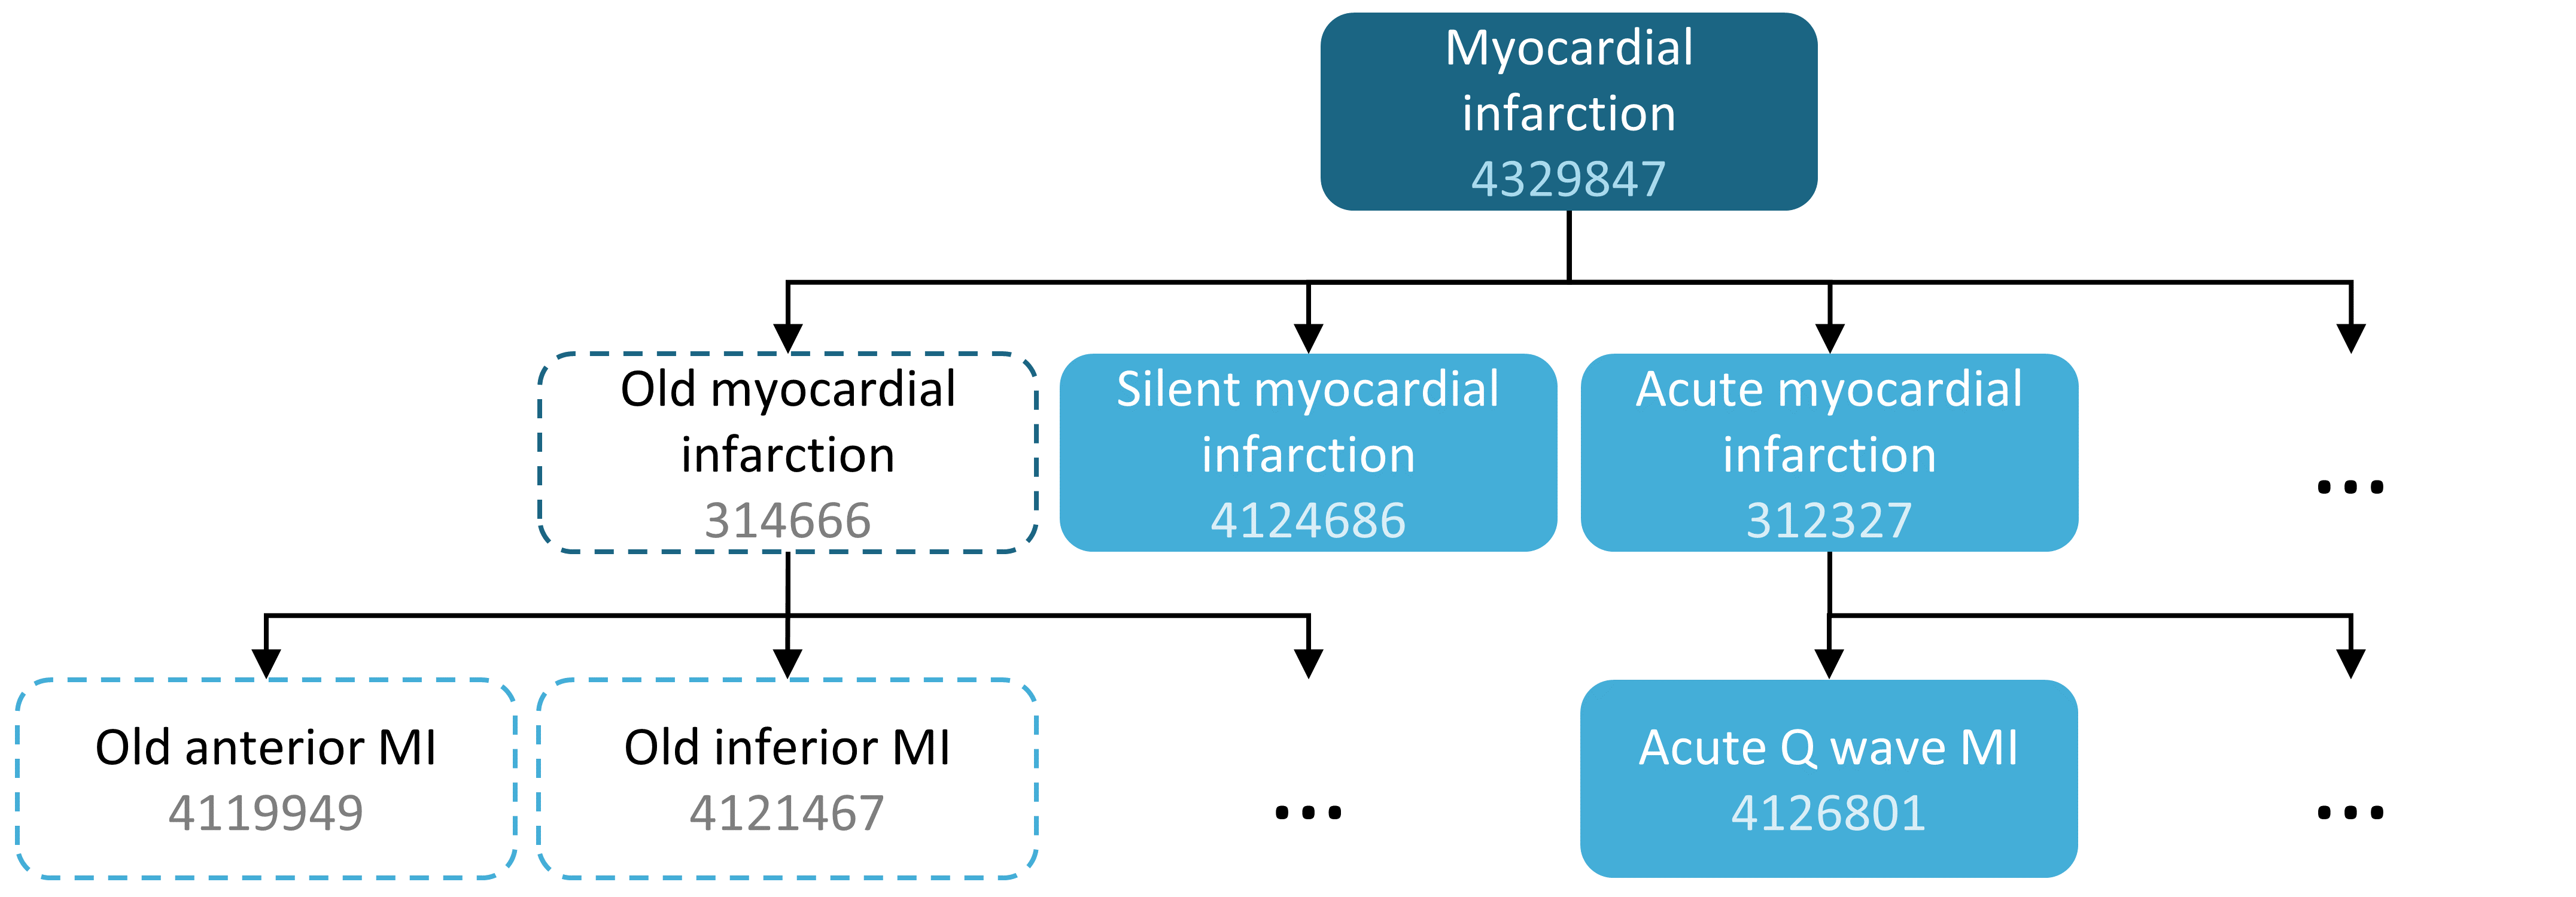
\includegraphics[width=1\linewidth]{images/Cohorts/conceptSet} 

}

\caption{「心筋梗塞」(下位層を含む)を含むが、「陳旧性心筋梗塞」(下位層を含む)を除外するコンセプトセット}\label{fig:conceptSet}
\end{figure}

\section{確率的コホート定義}\label{ux78baux7387ux7684ux30b3ux30dbux30fcux30c8ux5b9aux7fa9}

ルールベースのコホート定義は、コホート定義を組み立てるための一般的な方法です。しかし、研究コホートを作成するために必要な専門家の合意を集めることは非常に時間がかかります。確率的コホート設計は、コホート属性の選択を迅速化するための代替手段であり、機械主導の方法です。このアプローチでは、監督された機械学習により、表現型分類アルゴリズムがコホートメンバーシップに寄与する属性がどのようにラベル付けされた例(ケース)から学習します。次に、このアルゴリズムを使用して、表現型を定義する特性をより明確にし、表現型基準を変更する際に全体的な研究精度でどのようなトレードオフが発生するかを判断できます。 \index{cohort!probabilistic design}

このアプローチをCDMデータに適用する例は、APHRODITE(Automated PHenotype Routine for Observational Definition, Identification, Training and Evaluation)Rパッケージ\footnote{\url{https://github.com/OHDSI/Aphrodite}}です。このパッケージは、不完全にラベル付けされたデータから学習する能力を組み合わせたコホートビルディングフレームワークを提供します \citep{Banda2017APHRODITE} \index{APHRODITE}。

\section{コホート定義の妥当性}\label{ux30b3ux30dbux30fcux30c8ux5b9aux7fa9ux306eux59a5ux5f53ux6027}

コホートを構築する際には次のどちらが重要かを考慮すべきです:\emph{すべての該当患者を見つけることが重要か?} それとも \emph{確信を持てる患者のみを取り込むことが重要か?}

コホートの構築戦略は、専門家のコンセンサスが疾患をどのように定義するかの臨床的厳格性に依存します。これはつまり、正しいコホート設計はあなたが解答を求めている質問に依存するということです。すべてを取り入れるコホート定義を選択するか、OHDSIサイト全体で共有できる最小公約数を使用するか、またはその両者の妥協案を選ぶか。最終的には、研究者の判断により、対象コホートの適切な研究に必要な厳格性の閾値が決まります。

この章の冒頭で述べたように、コホート定義は記録されたデータから観察したいことを推測する試みです。それがどの程度うまくいったかという問いが生じます。一般に、ルールに基づくコホート定義や確率的アルゴリズムの検証は、提案されたコホートを「ゴールドスタンダード」の参考文献(例: ケースの手動チャートレビュー)と比較する試験として考えられます。詳細はChapter \ref{ClinicalValidity}(「臨床的妥当性」)に記載されています。

\subsection{OHDSI ゴールドスタンダード表現型ライブラリ}\label{ohdsi-ux30b4ux30fcux30ebux30c9ux30b9ux30bfux30f3ux30c0ux30fcux30c9ux8868ux73feux578bux30e9ux30a4ux30d6ux30e9ux30ea}

既存のコホート定義とアルゴリズムの在庫と全体的な評価を支援するために、OHDSI ゴールドスタンダード表現型ライブラリ(GSPL)ワークグループが設立されました。GSPLワークグループの目的は、ルールベースおよび確率的手法からのコミュニティ支援のフェノタイプライブラリを開発することです。GSPLにより、OHDSIコミュニティのメンバーは、コミュニティによって妥当性が確認されたコホート定義を研究やその他の活動に利用することができます。これらの「ゴールドスタンダード」定義は特定の設計と評価基準に従ってライブラリに保存されます。GSPLに関連する追加情報はOHDSIワークグループページを参照してください\footnote{\url{https://www.ohdsi.org/web/wiki/doku.php?id=projects:workgroups:gold-library-wg}}。 このワークグループの研究には、先のセクションで議論されたAPHRODITE \citep{Banda2017APHRODITE} およびPheValuatorツール \citep{Swerdel2019phevaluator} の他、OHDSIネットワーク全体での電子カルテおよびゲノミクスの \href{https://emerge.mc.vanderbilt.edu/}{eMERGE} \href{https://phekb.org/phenotypes}{Phenotype Library} の共有に関する作業も含まれます \citep{Hripcsak2019eMERGE}。表現型のキュレーションに関心がある場合は、このワークグループに貢献することを考えてみてください。 \index{phenotype library}

\section{高血圧のコホート定義}\label{ux9ad8ux8840ux5727ux306eux30b3ux30dbux30fcux30c8ux5b9aux7fa9}

コホート定義をルールベースのアプローチでまとめることによって、コホートスキルを練習し始めます。この例では、\emph{高血圧の初期治療としてACE阻害薬を単剤療法で開始する患者}を見つけたいと考えます。

このコンテキストを念頭に、コホートを構築します。この演習を通して、標準的な減少チャートに似た方法でコホートを構築します。図 \ref{fig:CohortPractice} は、このコホートをどのように構築するかの論理的なフレームワークを示しています。

\begin{figure}

{\centering 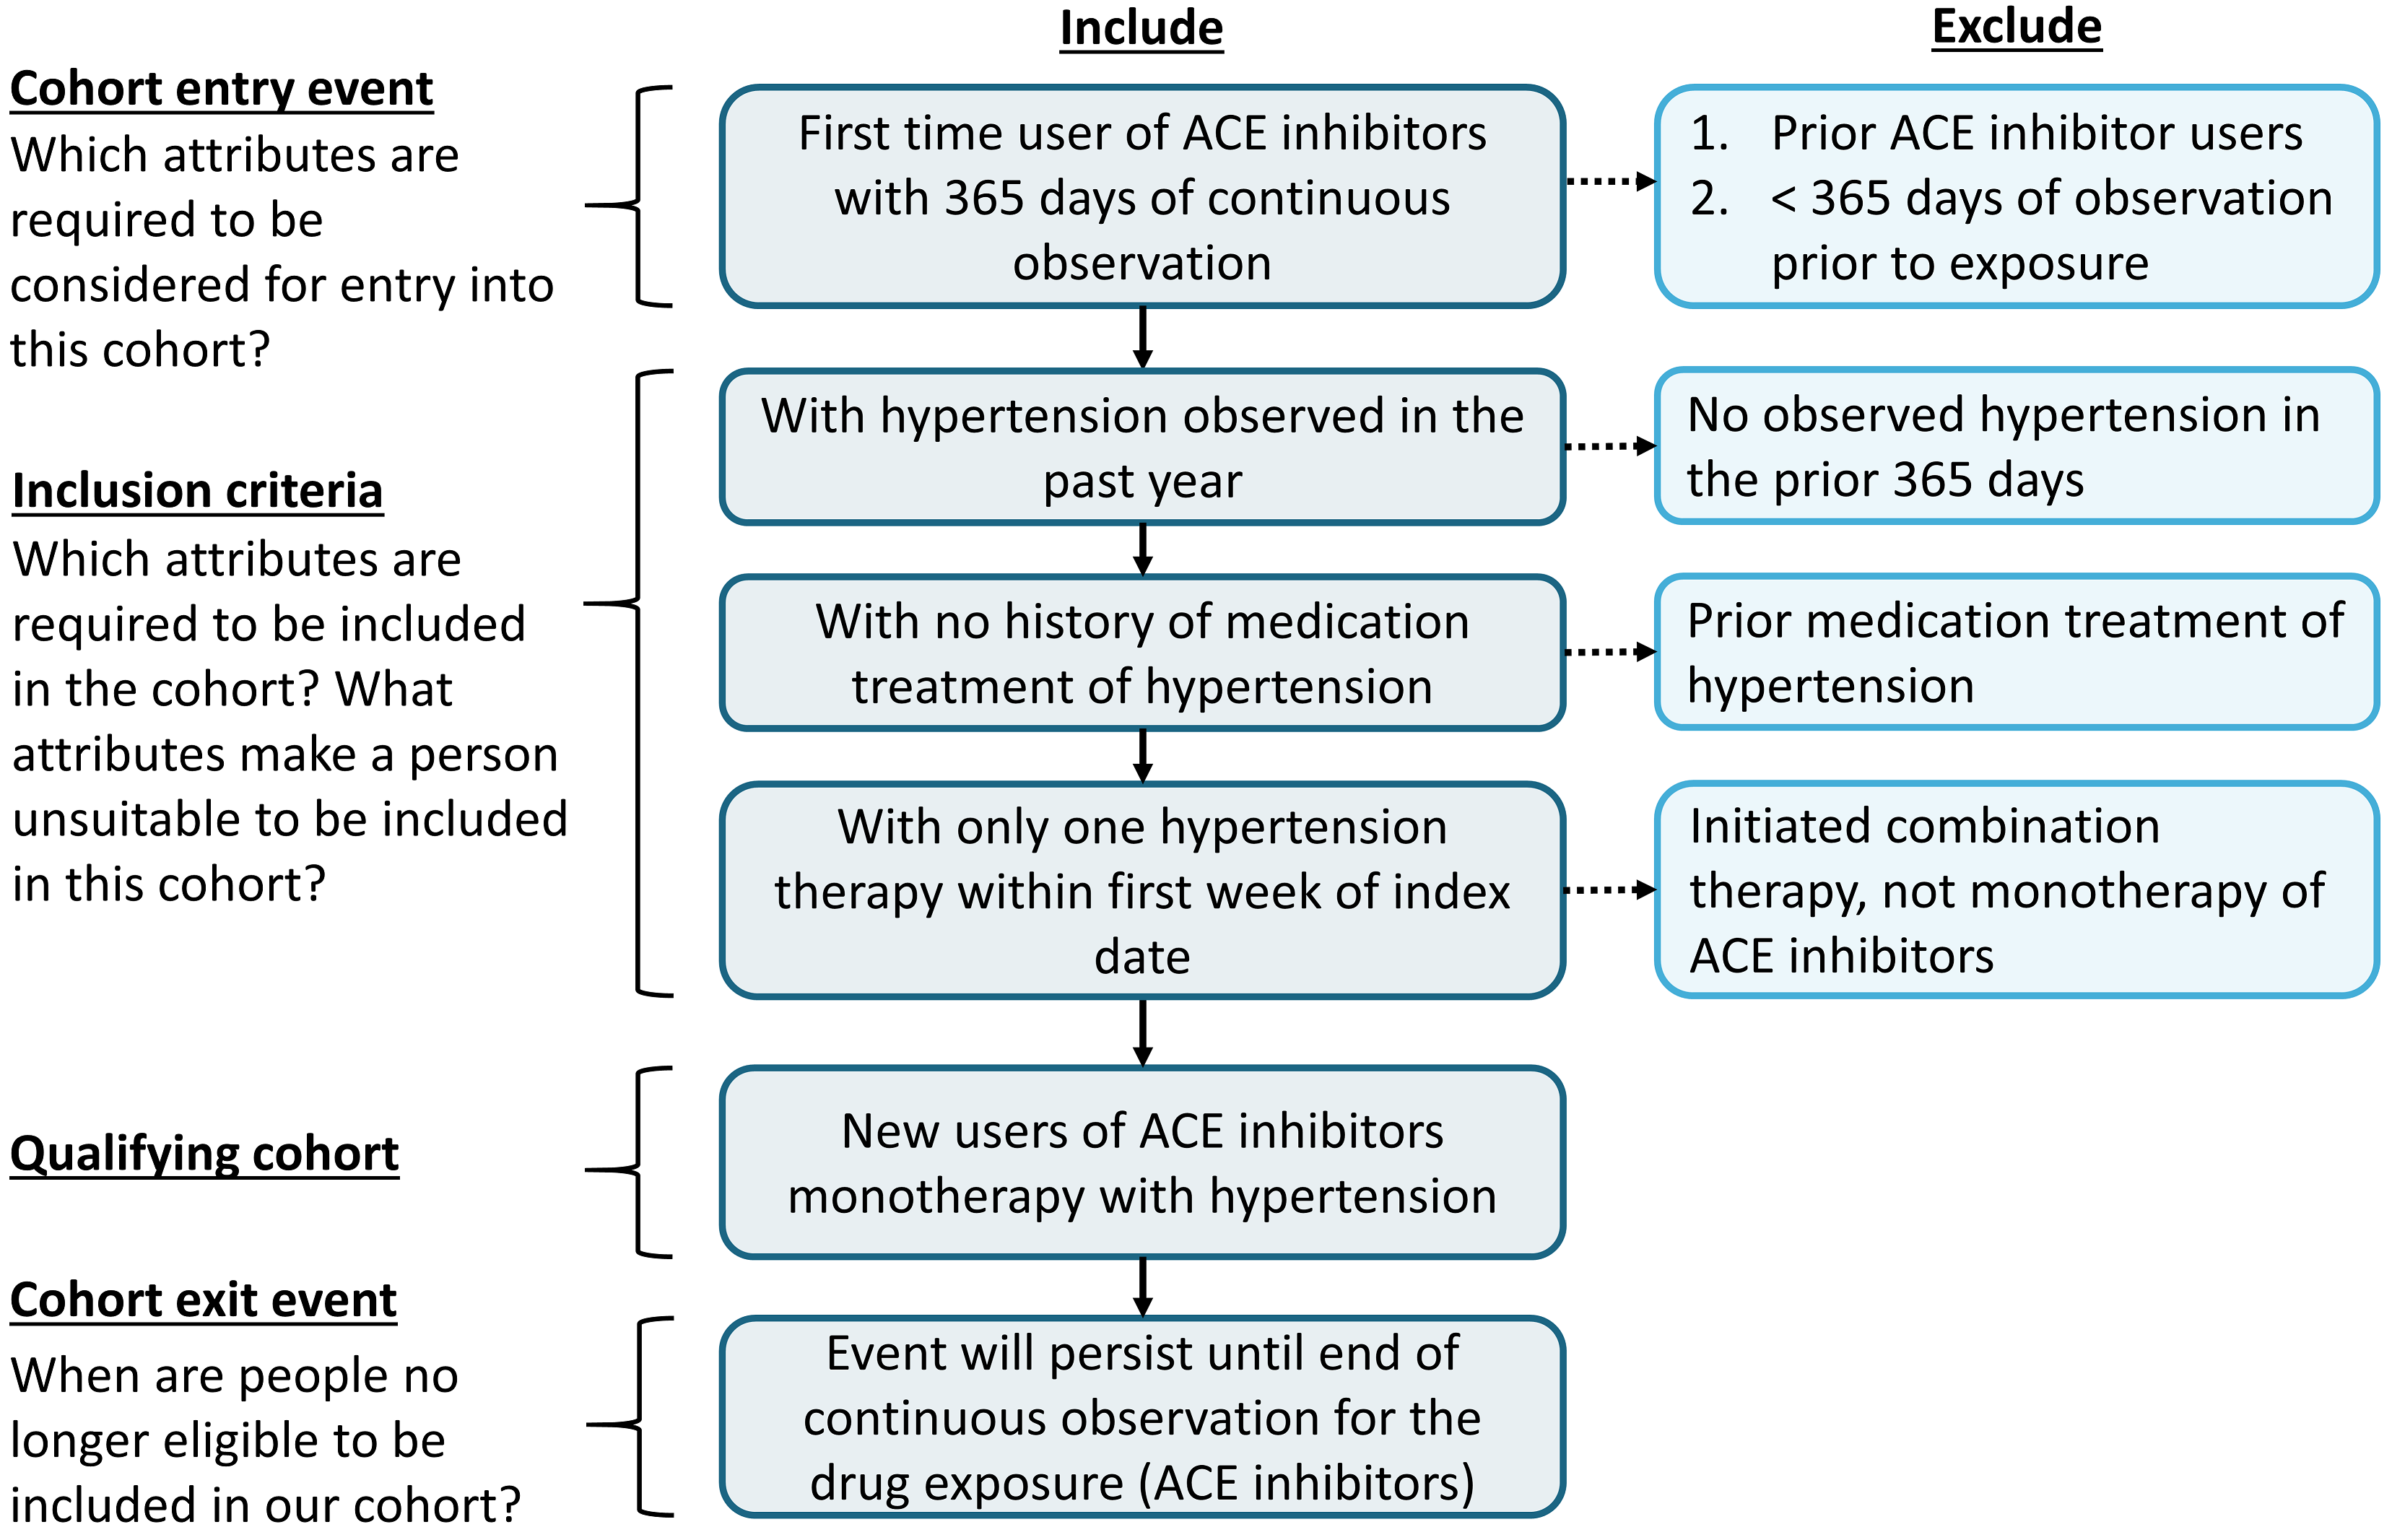
\includegraphics[width=1\linewidth]{images/Cohorts/CohortPractice} 

}

\caption{目標とするコホートの論理図}\label{fig:CohortPractice}
\end{figure}

コホートはATLASのユーザーインターフェースで作成することも、CDMに対して直接クエリを記述することもできます。この章では、これらの両方について簡単に説明します。

\section{ATLASを用いたコホートの実装}\label{atlasux3092ux7528ux3044ux305fux30b3ux30dbux30fcux30c8ux306eux5b9fux88c5}

まずATLASで始めるには、
\includegraphics{images/Cohorts/cohortdefinition.png}モジュールをクリックします。モジュールが読み込まれると、「New cohort」をクリックします。次の画面では空のコホート定義が表示されます。図\ref{fig:ATLASdefineacohort}に示す内容が画面に表示されます。

\begin{figure}

{\centering 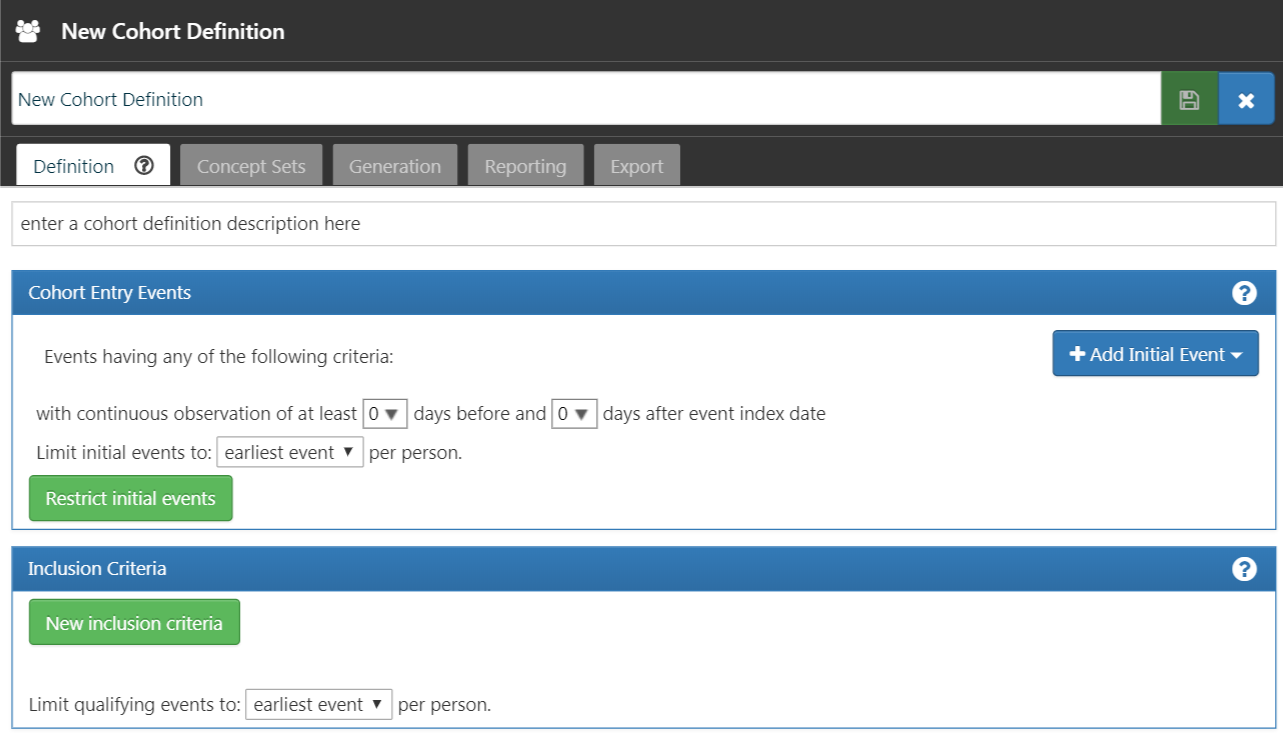
\includegraphics[width=1\linewidth]{images/Cohorts/ATLAS-defineacohort} 

}

\caption{新しいコホート定義}\label{fig:ATLASdefineacohort}
\end{figure}

まず最初に、「New Cohort Definition」からコホートの名前を自身のユニークな名前に変更することをお勧めします。「高血圧に対する第一選択単剤療法としてのACE阻害薬の新規ユーザー」のような名前を付けることができます。

\begin{rmdimportant}
ATLASは二つのコホートが全く同じ名前を持つことを許可しません。他のATLASコホートで既に使われている名前を選んだ場合、ATLASはポップアップエラーメッセージを表示します。
\end{rmdimportant}

名前を決めたら、
\includegraphics{images/Cohorts/save.png}をクリックしてコホートを保存します。

\subsection{初期イベント基準}\label{ux521dux671fux30a4ux30d9ux30f3ux30c8ux57faux6e96}

では、初期コホートイベントの定義を進めます。「Add initial event」をクリックします。どのドメインに基づいて基準を設定するかを選ばなければなりません。「どのドメインが初期コホートイベントかどうかをどのように知るのか?」という疑問を抱くかも知れません。これを解決しましょう。

\begin{figure}

{\centering 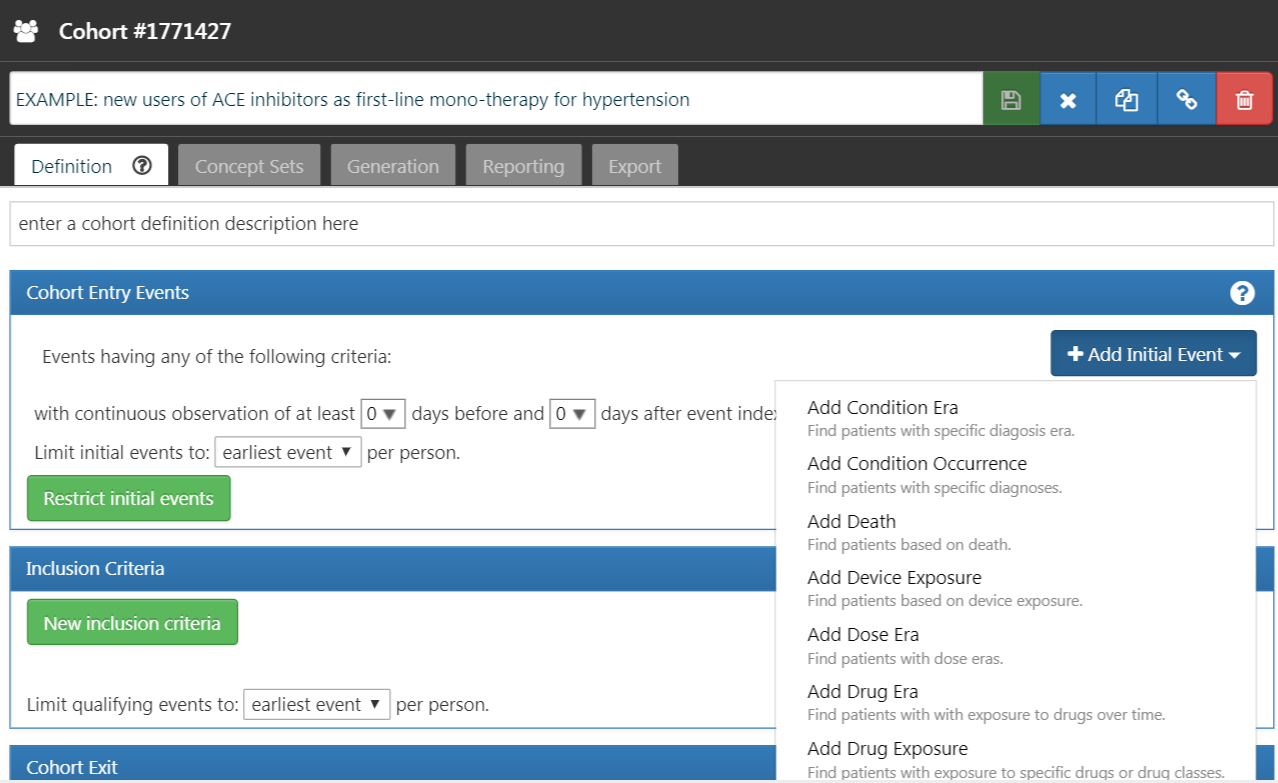
\includegraphics[width=1\linewidth]{images/Cohorts/ATLAS-initialevent} 

}

\caption{初期イベントの追加}\label{fig:ATLASinitialevent}
\end{figure}

図\ref{fig:ATLASinitialevent}に示されているように、ATLASは各基準の説明を提供しています。もしCONDITION\_OCCURRENCEに基づいた基準を構築している場合、特定の診断を持つ患者を探しているということになります。DRUG\_EXPOSUREに基づいた基準を構築している場合、特定の薬または薬クラスを持つ患者を探しているということになります。高血圧に対する第一選択治療としてACE阻害薬単剤療法を開始する患者を見つけるため、DRUG\_EXPOSURE基準を選択します。あなたが「しかし、高血圧としての診断も重要では?」と思うかも知れません。それは正しいです。高血圧は我々が構築する他の基準です。しかし、コホートの開始日はACE阻害薬治療の開始によって定義されるため、それが初期イベントです。高血圧の診断は、\emph{追加の資格基準}と呼ばれるものです。この基準を構築した後で再度考慮します。「Add Drug Exposure」をクリックします。

画面は選択した基準を表示するように更新されますが、まだ終了ではありません。図\ref{fig:ATLASdrugexposure}を参照すると、ATLASはどの薬を探しているのかを知りません。ATLASにACE阻害薬に関連するコンセプトセットを知らせる必要があります。

\begin{figure}

{\centering 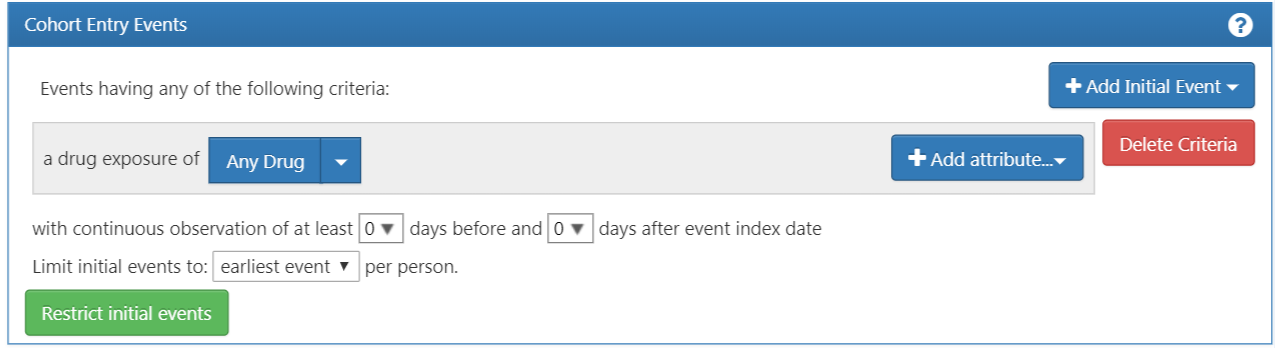
\includegraphics[width=1\linewidth]{images/Cohorts/ATLAS-drugexposure} 

}

\caption{薬剤曝露の定義}\label{fig:ATLASdrugexposure}
\end{figure}

\subsection{コンセプトセットの定義}\label{ux30b3ux30f3ux30bbux30d7ux30c8ux30bbux30c3ux30c8ux306eux5b9aux7fa9}

コンセプトセットを定義するためには、
\includegraphics{images/Cohorts/downarrow.png}をクリックして、ACE阻害薬を定義するためのコンセプトセットを取得するダイアログボックスを開きます。

\subsubsection*{シナリオ1: コンセプトセットを構築していない場合}\label{ux30b7ux30caux30eaux30aa1-ux30b3ux30f3ux30bbux30d7ux30c8ux30bbux30c3ux30c8ux3092ux69cbux7bc9ux3057ux3066ux3044ux306aux3044ux5834ux5408}
\addcontentsline{toc}{subsubsection}{シナリオ1: コンセプトセットを構築していない場合}

基準に適用するためのコンセプトセットを集めていない場合は、先にそれを行う必要があります。コホート定義内で「Concept set」タブに移動し、「New Concept Set」をクリックしてコンセプトセットを構築することができます。「Unnamed Concept Set」から任意の名前に変更する必要があります。そこから、
\includegraphics{images/Cohorts/search-2.png}モジュールを使用してACE阻害薬を表す臨床コンセプトを検索できます(図\ref{fig:aceinhibitors}を参照)。

\begin{figure}

{\centering 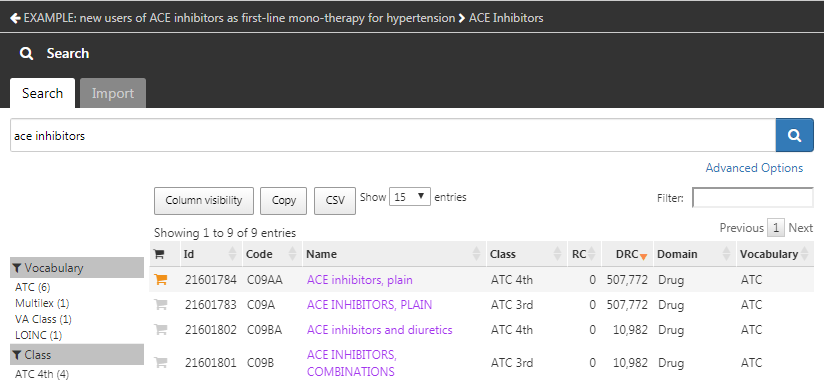
\includegraphics[width=1\linewidth]{images/Cohorts/aceinhibitors} 

}

\caption{語彙の検索 - ACE阻害薬}\label{fig:aceinhibitors}
\end{figure}

使用したい用語を見つけたら、\includegraphics{images/Cohorts/shoppingcart.png}をクリックしてコンセプトを選択します。図\ref{fig:aceinhibitors}の左矢印を使用してコホート定義に戻ります。興味のある臨床コンセプトを見つけるための語彙のナビゲートは、チャプター\ref{StandardizedVocabularies}(標準化された語彙)に参照できます。

図\ref{fig:aceConceptSetExpression}は私たちのコンセプトセット表現を示しています。興味のあるすべてのACE阻害薬成分を選び、その子孫すべてを含め、これらの成分を含むすべての薬を含めています。「Included concepts」をクリックして、この表現に含まれている21,536のコンセプトすべてを確認することができ、「Included Source Codes」をクリックして様々なコーディングシステムに含まれているすべてのソースコードを調査できます。

\begin{figure}

{\centering \includegraphics[width=1\linewidth]{images/Cohorts/aceConceptSetExpression} 

}

\caption{ACE阻害薬を含むコンセプトセット}\label{fig:aceConceptSetExpression}
\end{figure}

\subsubsection*{シナリオ2: すでにコンセプトセットを構築している場合}\label{ux30b7ux30caux30eaux30aa2-ux3059ux3067ux306bux30b3ux30f3ux30bbux30d7ux30c8ux30bbux30c3ux30c8ux3092ux69cbux7bc9ux3057ux3066ux3044ux308bux5834ux5408}
\addcontentsline{toc}{subsubsection}{シナリオ2: すでにコンセプトセットを構築している場合}

すでにコンセプトセットを作成してATLASに保存している場合、「Import Concept Set」をクリックします。ダイアログボックスが開き、ATLASのコンセプトセットリポジトリからコンセプトを見つけるように促されます(図\ref{fig:ATLASfindyourconcept}を参照)。例の図ではユーザーはATLASに保存されているコンセプトセットを取得しています。右側の検索に「ace inhibitors」と入力し、コンセプトセットのリストがマッチングする名前のコンセプトのみに絞り込まれます。そこからユーザーはコンセプトセットの行をクリックして選択します。(注意: コンセプトセットを選択するとダイアログボックスは消えます。)選択したコンセプトセットの名前が「Any Drug」ボックスに更新されると、この操作が成功したことがわかります。

\begin{figure}

{\centering \includegraphics[width=1\linewidth]{images/Cohorts/ATLAS-findingyourconcept} 

}

\caption{ATLASリポジトリからのコンセプトセットのインポート}\label{fig:ATLASfindyourconcept}
\end{figure}

\subsection{追加の初期イベント基準}\label{ux8ffdux52a0ux306eux521dux671fux30a4ux30d9ux30f3ux30c8ux57faux6e96}

コンセプトセットを添付したら、まだ終了ではありません。質問は新たにACE阻害薬を初めて使用するユーザーもしくは、ACE阻害薬に曝露した経験があるユーザーを探すものです。これは、患者の記録において初回のACE阻害薬曝露を表します。これを指定するには、「+Add attribute」をクリックします。次に「Add first exposure criteria」を選択します。注意:基準を構築する際に他の属性を指定することもできます。発生時の年齢、発生日、性別、薬剤に関連するその他の属性を指定できます。各ドメインの基準が異なることがあります。

選択したら、ウィンドウは自動的に閉じます。この追加属性は初期基準と同じボックスに表示されます(図\ref{fig:initialEventAce}を参照)。

\begin{rmdimportant}
現在のATLASのデザインは一部の人々を混乱させるかもしれません。見た目の通り、\includegraphics{images/Cohorts/redX.png}は「No」を意味するものではありません。これは、基準を削除するための操作可能な機能です。もし\includegraphics{images/Cohorts/redX.png}をクリックすると、この基準は消えます。したがって、基準を有効に保つには\includegraphics{images/Cohorts/redX.png}を残す必要があります。
\end{rmdimportant}

これで初期の検証イベントが構築できました。初回の薬剤曝露をキャプチャするため、見落しがないことを知るために、ルックバックウィンドウを追加する必要があります。観察期間の短い患者が非表示の曝露を受ける場合があるため、観察期間の最低限度を規定することができます。これにより、記録の最初の発生をキャプチャしていることを確認するために、患者の履歴を見る最低期間を設定できます。この基準は他コホートでも異なる基準を選択することができます。365日間の継続的な観察を初期イベント前に要求します。観察期間を更新して、初期イベント後0日として更新します。最初のACE阻害薬の使用であることを保証するために、「earliest event」を選択します。図\ref{fig:initialEventAce}を参照してロジックを確認してください。

\begin{figure}

{\centering \includegraphics[width=1\linewidth]{images/Cohorts/initialEventAce} 

}

\caption{インデックス日付前に必要な継続的観察を設定}\label{fig:initialEventAce}
\end{figure}

このロジックがどのように組み合わさるかを説明すると、患者のタイムラインを組み立てることを考えることができます。

\begin{figure}

{\centering \includegraphics[width=1\linewidth]{images/Cohorts/EarliestEventExplained} 

}

\caption{基準の適用による患者の適格性の説明}\label{fig:EarliestEventExplained}
\end{figure}

図\ref{fig:EarliestEventExplained}では、各ラインがコホートに参加資格がある可能性のある単一の患者を表しています。塗りつぶされた星は、患者が指定された基準を満たすタイミングを表しています。追加の基準が適用されると、いくつかの星がより薄い色になります。これは、これらの患者が基準を満たす他の記録を持っていることを意味しますが、その基準を満たす前に他の記録があることを意味します。最終的な基準に達するまでに、私たちは初めてのACE阻害薬使用とその前の365日間の連続する観察を持つ患者の累積ビューを見ています。論理的には、最初のイベントに限定することは冗長ですが、すべての選択で明確なロジックを維持することに役立ちます。独自のコホートを構築するときには、\href{http://forums.ohdsi.org}{OHDSIフォーラム}の研究者セクションに参加して、コホート論理の構築について第二の意見を得ることをお勧めします。

\subsection{選択基準}\label{ux9078ux629eux57faux6e96}

コホートエントリエベントを指定したら、追加の資格イベントを「Restrict initial events」または「New inclusion criteria」のいずれかに追加することができます。これら二つのオプション間の基本的な違いは、ATLASが提供する中間情報の内容です。「Restrict initial events」に追加基準を加えると、ATLASでカウントを生成するときに、これらすべての基準を満たす人の数だけが返されます。「New inclusion criteria」に基準を追加すると、追加の包括基準を適用することによって失う患者数を示す削減チャートが表示されます。各選択ルールがコホート定義の全体的な成功に与える影響を理解するために、包括基準セクションを利用することを強くお勧めします。特定の包括基準がコホートに入る人の数を大幅に制限する可能性があることがわかります。この段階では、コホートを大きくするためにこの基準を緩和する選択をするかもしれません。最終的には、このコホートを組み立てる専門家の合意に従います。

コホートのメンバーシップに関するロジックをさらに追加するために「New inclusion criteria」をクリックしてください。このセクションの機能は、前述のコホート基準の構築方法と同じです。私たちの最初の追加基準は次のとおりです:\emph{ACE阻害薬の最初の開始日から365日から0日以内の少なくとも1回の高血圧障害の発生がある患者のみ}。新しい包括基準を追加するには「New inclusion criteria」をクリックします。基準に名前を付け、必要に応じて探している内容についての簡単な説明を書き込むことができます。これは自分が定義している基準を覚えるためのもので、コホートの整合性に影響を与えるものではありません。

新しい基準に注釈を付けたら、「+Add criteria to group」ボタンをクリックして、このルールの実際の基準を構築します。このボタンは「Add Initial Event」と同様に機能します。ただし、初期イベントを指定するわけではありません。複数の基準を追加できるため、「add criteria to group」と指定されています。たとえば、病気を見つけるための複数の方法(例:CONDITION\_OCCURRENCEのロジック、この状態の代理としてのDRUG\_EXPOSUREのロジック、この状態の代理としてのMEASUREMENTのロジック)があります。これらは別々のドメインであり、異なる基準を必要としますが、この状態を探すための1つの基準にグループ化できます。

この場合、高血圧症の診断を見つけたいので、「条件の発生」を追加します。このレコードに概念セットを添付することで、最初のイベントと同様の手順に従います。また、イベントがインデックス日(最初のACE阻害薬の使用)の365日前から0日後までの間に開始したことを指定します。次に、図 \citet{ref}(fig:ATLASIC1) に対してロジックを確認します。

\begin{figure}

{\centering \includegraphics[width=1\linewidth]{images/Cohorts/ATLAS-IC1} 

}

\caption{追加の選択基準 1}\label{fig:ATLASIC1}
\end{figure}

次に、患者を検索するための別の条件を追加します:\emph{インデックス開始日の前日から当日までの全期間において、高血圧治療薬の使用歴がまったくない(ACE阻害薬の使用開始以前に高血圧治療薬を使用していない)}。このプロセスは、以前と同様に''New inclusion criteria (新規の選択基準)``ボタンをクリックし、この条件に注釈を追加し、''+Add criteria to group (グループに条件を追加)``をクリックすると開始されます。これは DRUG\_EXPOSURE なので、''Add Drug Exposure (薬剤曝露を追加)``をクリックし、高血圧治療薬のコンセプトセットを添付し、インデックス日から遡るすべての日とインデックス日0日後の間(または図で示されているように「1日前」も同様)を指定します。選択した発生回数が \emph{正確に 0} であることを確認してください。 図 \ref{fig:ATLASIC2} で、ロジックを確認してください。

\begin{figure}

{\centering \includegraphics[width=1\linewidth]{images/Cohorts/ATLAS-IC2} 

}

\caption{追加の選択基準 2}\label{fig:ATLASIC2}
\end{figure}

「出現なし」が「正確に0回出現」としてコード化される理由がわからないかもしれません。これは、ATLASが知識を咀嚼する方法のニュアンスです。ATLAS は選択条件のみを処理します。特定の属性が存在しないことを指定する場合は、論理演算子を使用する必要があります。例えば、「正確に0回」などです。ATLASの選択基準で使用できる論理演算子については、徐々に理解が深まるでしょう。

最後に、患者を検索するために、もう一つ別の条件を追加します:\emph{インデックス開始日の0日前から7日後までの間に高血圧治療薬が1回だけ処方されていること、かつ、高血圧治療薬(ACE阻害薬)を1種類しか処方されていないこと}。このプロセスは、前回と同様に''New inclusion criteria (新しい選択基準)``ボタンをクリックし、この条件に注釈を追加してから''+Add criteria to group (グループに条件を追加)``をクリックすると開始されます。これは DRUG\_ERA なので、''Add Drug Era (薬剤曝露期間を追加)``をクリックし、高血圧治療薬のコンセプトセットを添付し、インデックス日の前0日および後7日を指定します。次に、図 \ref{fig:ATLASIC3} と照らし合わせてロジックを確認します。

\begin{figure}

{\centering \includegraphics[width=1\linewidth]{images/Cohorts/ATLAS-IC3} 

}

\caption{追加の選択基準 3}\label{fig:ATLASIC3}
\end{figure}

\subsection{コホート・エグジット基準}\label{ux30b3ux30dbux30fcux30c8ux30a8ux30b0ux30b8ux30c3ux30c8ux57faux6e96}

これで、すべての適格な選択基準が追加されました。次に、コホート・エグジット基準を指定する必要があります。「このコホートに含まれる対象ではなくなるのはどのような場合か?」と問うことになります。このコホートでは、薬剤曝露を受けた新規ユーザーを追跡しています。薬剤曝露に関連する継続的な観察期間を調べたいと考えています。そのため、コホート・エグジット基準、継続的な薬剤曝露の全般について適用されるように指定します。その後、薬剤への曝露が中断された場合は、その時点で患者はコホートから退出します。薬剤への曝露が中断された間の患者の状態が不明であるため、このような措置を取っています。また、薬剤への曝露間の許容可能なギャップを特定する持続ウィンドウの基準を設定することもできます。このケースでは、持続曝露の時期を推定する際に、曝露レコードの間の最大許容期間は30日間であると、この研究を主導する専門家が結論づけました。

\textbf{なぜギャップが許容されるのでしょうか?} データセットによっては、受療の一部しか観察できないことがあります。特に薬物曝露は、一定期間をカバーする処方箋の調剤を表している可能性があります。そのため、調剤単位が1日を超えているため、患者は論理的には依然として最初の薬物曝露を受けられる可能性があることを考慮し、薬物曝露の間には一定の時間的余裕を設けるようにしています。

これを設定するには、イベントは''end of a continuous drug exposure (連続した薬剤曝露の終了)'' まで継続するを選択します。次に、持続期間を''allow for a maximum of 30 days (最大30日間)``に設定し、「ACE阻害剤」のコンセプトセットを追加します。図 \ref{fig:ATLAScohortexit} と照らし合わせてロジックを確認しましょう。

\begin{figure}

{\centering \includegraphics[width=1\linewidth]{images/Cohorts/cohort-exit} 

}

\caption{コホート・エグジット基準}\label{fig:ATLAScohortexit}
\end{figure}

このコホートの場合、他に打ち切りイベントはありません。しかし、打ち切りを指定する必要があるようなコホートを作成することもあるかもしれません。その場合には、コホート定義に他の属性を追加したのと同様の手順で作業を進めます。これで、コホートの作成が完了しました。\includegraphics{images/Cohorts/save.png} ボタンをクリックしてください。おめでとうございます!コホートの作成は、OHDSIツールでリサーチ・クエスチョンに答えるための最も重要な構成要素です。``Export (出力)'' タブを使用して、SQLコードまたはATLASに読み込むためのJSONファイルの形式により、他の共同研究者とコホート定義を共有することができます。

\section{SQLを使用したコホートの実装}\label{sqlux3092ux4f7fux7528ux3057ux305fux30b3ux30dbux30fcux30c8ux306eux5b9fux88c5}

ここでは、SQLとRを使用して同じコホートを作成する方法について説明します。第\ref{SqlAndR}章で説明したように、OHDSIはSqlRenderとDatabaseConnectorという2つのRパッケージを提供しており、これらを組み合わせることで、多様なデータベースプラットフォームに対して自動的に翻訳・実行されるSQLコードを記述できます。

理解しやすさのために、SQLをいくつかのチャンクに分割し、各チャンクが次のチャンクで使用される一時テーブルを生成するようにします。これはおそらく最も計算効率の良い方法ではありませんが、非常に長い一つのステートメントよりも読みやすくなります。

\subsection{データベースへの接続}\label{ux30c7ux30fcux30bfux30d9ux30fcux30b9ux3078ux306eux63a5ux7d9a-1}

最初にRに対してサーバーへの接続方法を指示する必要があります。これには\href{https://ohdsi.github.io/DatabaseConnector/}{DatabaseConnector}パッケージを使用し、\texttt{createConnectionDetails}という名前の関数を提供します。各データベース管理システム(DBMS)に必要な具体的な設定については、\texttt{?createConnectionDetails}と入力してください。例えば、以下のコードでPostgreSQLデータベースに接続することができます:

\begin{Shaded}
\begin{Highlighting}[]
\FunctionTok{library}\NormalTok{(CohortMethod)}
\NormalTok{connDetails }\OtherTok{\textless{}{-}} \FunctionTok{createConnectionDetails}\NormalTok{(}\AttributeTok{dbms =} \StringTok{"postgresql"}\NormalTok{,}
                                       \AttributeTok{server =} \StringTok{"localhost/ohdsi"}\NormalTok{,}
                                       \AttributeTok{user =} \StringTok{"joe"}\NormalTok{,}
                                       \AttributeTok{password =} \StringTok{"supersecret"}\NormalTok{)}

\NormalTok{cdmDbSchema }\OtherTok{\textless{}{-}} \StringTok{"my\_cdm\_data"}
\NormalTok{cohortDbSchema }\OtherTok{\textless{}{-}} \StringTok{"scratch"}
\NormalTok{cohortTable }\OtherTok{\textless{}{-}} \StringTok{"my\_cohorts"}
\end{Highlighting}
\end{Shaded}

最後の3行で、\texttt{cdmDbSchema}、\texttt{cohortDbSchema}、および\texttt{cohortTable}の変数を定義しています。これらは後で、CDM形式のデータが存在する場所と、興味のあるコホートを作成する場所をRに伝えるために使用します。Microsoft SQL Serverの場合、データベースのスキーマはデータベースとスキーマの両方を指定する必要があることに注意してください。例:\texttt{cdmDbSchema\ \textless{}-\ "my\_cdm\_data.dbo"}。

\subsection{コンセプトの指定}\label{ux30b3ux30f3ux30bbux30d7ux30c8ux306eux6307ux5b9a}

読みやすさのために、必要なコンセプトIDをRで定義し、それらをSQLに渡します:

\begin{Shaded}
\begin{Highlighting}[]
\NormalTok{aceI }\OtherTok{\textless{}{-}} \FunctionTok{c}\NormalTok{(}\DecValTok{1308216}\NormalTok{, }\DecValTok{1310756}\NormalTok{, }\DecValTok{1331235}\NormalTok{, }\DecValTok{1334456}\NormalTok{, }\DecValTok{1335471}\NormalTok{, }\DecValTok{1340128}\NormalTok{, }\DecValTok{1341927}\NormalTok{,}
          \DecValTok{1342439}\NormalTok{, }\DecValTok{1363749}\NormalTok{, }\DecValTok{1373225}\NormalTok{)}

\NormalTok{hypertension }\OtherTok{\textless{}{-}} \DecValTok{316866}

\NormalTok{allHtDrugs }\OtherTok{\textless{}{-}} \FunctionTok{c}\NormalTok{(}\DecValTok{904542}\NormalTok{, }\DecValTok{907013}\NormalTok{, }\DecValTok{932745}\NormalTok{, }\DecValTok{942350}\NormalTok{, }\DecValTok{956874}\NormalTok{, }\DecValTok{970250}\NormalTok{, }\DecValTok{974166}\NormalTok{,}
                  \DecValTok{978555}\NormalTok{, }\DecValTok{991382}\NormalTok{, }\DecValTok{1305447}\NormalTok{, }\DecValTok{1307046}\NormalTok{, }\DecValTok{1307863}\NormalTok{, }\DecValTok{1308216}\NormalTok{,}
                  \DecValTok{1308842}\NormalTok{, }\DecValTok{1309068}\NormalTok{, }\DecValTok{1309799}\NormalTok{, }\DecValTok{1310756}\NormalTok{, }\DecValTok{1313200}\NormalTok{, }\DecValTok{1314002}\NormalTok{,}
                  \DecValTok{1314577}\NormalTok{, }\DecValTok{1317640}\NormalTok{, }\DecValTok{1317967}\NormalTok{, }\DecValTok{1318137}\NormalTok{, }\DecValTok{1318853}\NormalTok{, }\DecValTok{1319880}\NormalTok{,}
                  \DecValTok{1319998}\NormalTok{, }\DecValTok{1322081}\NormalTok{, }\DecValTok{1326012}\NormalTok{, }\DecValTok{1327978}\NormalTok{, }\DecValTok{1328165}\NormalTok{, }\DecValTok{1331235}\NormalTok{,}
                  \DecValTok{1332418}\NormalTok{, }\DecValTok{1334456}\NormalTok{, }\DecValTok{1335471}\NormalTok{, }\DecValTok{1338005}\NormalTok{, }\DecValTok{1340128}\NormalTok{, }\DecValTok{1341238}\NormalTok{,}
                  \DecValTok{1341927}\NormalTok{, }\DecValTok{1342439}\NormalTok{, }\DecValTok{1344965}\NormalTok{, }\DecValTok{1345858}\NormalTok{, }\DecValTok{1346686}\NormalTok{, }\DecValTok{1346823}\NormalTok{,}
                  \DecValTok{1347384}\NormalTok{, }\DecValTok{1350489}\NormalTok{, }\DecValTok{1351557}\NormalTok{, }\DecValTok{1353766}\NormalTok{, }\DecValTok{1353776}\NormalTok{, }\DecValTok{1363053}\NormalTok{,}
                  \DecValTok{1363749}\NormalTok{, }\DecValTok{1367500}\NormalTok{, }\DecValTok{1373225}\NormalTok{, }\DecValTok{1373928}\NormalTok{, }\DecValTok{1386957}\NormalTok{, }\DecValTok{1395058}\NormalTok{,}
                  \DecValTok{1398937}\NormalTok{, }\DecValTok{40226742}\NormalTok{, }\DecValTok{40235485}\NormalTok{)}
\end{Highlighting}
\end{Shaded}

\subsection{初回使用の発見}\label{ux521dux56deux4f7fux7528ux306eux767aux898b}

まず、各患者のACE阻害薬の初回使用を見つけます:

\begin{Shaded}
\begin{Highlighting}[]
\NormalTok{conn }\OtherTok{\textless{}{-}} \FunctionTok{connect}\NormalTok{(connDetails)}

\NormalTok{sql }\OtherTok{\textless{}{-}} \StringTok{"SELECT person\_id AS subject\_id,}
\StringTok{  MIN(drug\_exposure\_start\_date) AS cohort\_start\_date}
\StringTok{INTO \#first\_use}
\StringTok{FROM @cdm\_db\_schema.drug\_exposure}
\StringTok{INNER JOIN @cdm\_db\_schema.concept\_ancestor}
\StringTok{  ON descendant\_concept\_id = drug\_concept\_id}
\StringTok{WHERE ancestor\_concept\_id IN (@ace\_i)}
\StringTok{GROUP BY person\_id;"}

\FunctionTok{renderTranslateExecuteSql}\NormalTok{(conn,}
\NormalTok{                          sql,}
                          \AttributeTok{cdm\_db\_schema =}\NormalTok{ cdmDbSchema,}
                          \AttributeTok{ace\_i =}\NormalTok{ aceI)}
\end{Highlighting}
\end{Shaded}

DRUG\_EXPOSUREテーブルをCONCEPT\_ANCESTORテーブルと結合することで、ACE阻害薬を含むすべての薬を見つけていることに注意してください。

\subsection{365日の事前観察が必要}\label{ux65e5ux306eux4e8bux524dux89b3ux5bdfux304cux5fc5ux8981}

次に、OBSERVATION\_PERIODテーブルと結合して365日間の連続した事前の観察が必要です:

\begin{Shaded}
\begin{Highlighting}[]
\NormalTok{sql }\OtherTok{\textless{}{-}} \StringTok{"SELECT subject\_id,}
\StringTok{  cohort\_start\_date}
\StringTok{INTO \#has\_prior\_obs}
\StringTok{FROM \#first\_use}
\StringTok{INNER JOIN @cdm\_db\_schema.observation\_period}
\StringTok{  ON subject\_id = person\_id}
\StringTok{    AND observation\_period\_start\_date \textless{}= cohort\_start\_date}
\StringTok{    AND observation\_period\_end\_date \textgreater{}= cohort\_start\_date}
\StringTok{WHERE DATEADD(DAY, 365, observation\_period\_start\_date) \textless{} cohort\_start\_date;"}

\FunctionTok{renderTranslateExecuteSql}\NormalTok{(conn, sql, }\AttributeTok{cdm\_db\_schema =}\NormalTok{ cdmDbSchema)}
\end{Highlighting}
\end{Shaded}

\subsection{高血圧の前診断が必要}\label{ux9ad8ux8840ux5727ux306eux524dux8a3aux65adux304cux5fc5ux8981}

365日前に高血圧の診断が必要です:

\begin{Shaded}
\begin{Highlighting}[]
\NormalTok{sql }\OtherTok{\textless{}{-}} \StringTok{"SELECT DISTINCT subject\_id,}
\StringTok{  cohort\_start\_date}
\StringTok{INTO \#has\_ht}
\StringTok{FROM \#has\_prior\_obs}
\StringTok{INNER JOIN @cdm\_db\_schema.condition\_occurrence}
\StringTok{  ON subject\_id = person\_id}
\StringTok{    AND condition\_start\_date \textless{}= cohort\_start\_date}
\StringTok{    AND condition\_start\_date \textgreater{}= DATEADD(DAY, {-}365, cohort\_start\_date)}
\StringTok{INNER JOIN @cdm\_db\_schema.concept\_ancestor}
\StringTok{  ON descendant\_concept\_id = condition\_concept\_id}
\StringTok{WHERE ancestor\_concept\_id = @hypertension;"}

\FunctionTok{renderTranslateExecuteSql}\NormalTok{(conn,}
\NormalTok{                          sql,}
                          \AttributeTok{cdm\_db\_schema =}\NormalTok{ cdmDbSchema,}
                          \AttributeTok{hypertension =}\NormalTok{ hypertension)}
\end{Highlighting}
\end{Shaded}

過去に複数の高血圧診断がある場合でも、重複するコホートエントリーを作成しないように\texttt{SELECT\ DISTINCT}を使用していることに注意してください。

\subsection{治療の無前使用が必要}\label{ux6cbbux7642ux306eux7121ux524dux4f7fux7528ux304cux5fc5ux8981}

高血圧治療の過去の使用がないことが必要です:

\begin{Shaded}
\begin{Highlighting}[]
\NormalTok{sql }\OtherTok{\textless{}{-}} \StringTok{"SELECT subject\_id,}
\StringTok{  cohort\_start\_date}
\StringTok{INTO \#no\_prior\_ht\_drugs}
\StringTok{FROM \#has\_ht}
\StringTok{LEFT JOIN (}
\StringTok{  SELECT *}
\StringTok{  FROM @cdm\_db\_schema.drug\_exposure}
\StringTok{  INNER JOIN @cdm\_db\_schema.concept\_ancestor}
\StringTok{    ON descendant\_concept\_id = drug\_concept\_id}
\StringTok{  WHERE ancestor\_concept\_id IN (@all\_ht\_drugs)}
\StringTok{) ht\_drugs}
\StringTok{  ON subject\_id = person\_id}
\StringTok{    AND drug\_exposure\_start\_date \textless{} cohort\_start\_date}
\StringTok{WHERE person\_id IS NULL;"}

\FunctionTok{renderTranslateExecuteSql}\NormalTok{(conn,}
\NormalTok{                          sql,}
                          \AttributeTok{cdm\_db\_schema =}\NormalTok{ cdmDbSchema,}
                          \AttributeTok{all\_ht\_drugs =}\NormalTok{ allHtDrugs)}
\end{Highlighting}
\end{Shaded}

LEFT JOINを使用しており、DRUG\_EXPOSUREテーブルからのperson\_idがNULLの場合のみ行を許可することに注意してください。

\subsection{単剤療法}\label{ux5358ux5264ux7642ux6cd5}

コホートエントリーの最初の7日間に高血圧治療への一回のみの曝露が必要です:

\begin{Shaded}
\begin{Highlighting}[]
\NormalTok{sql }\OtherTok{\textless{}{-}} \StringTok{"SELECT subject\_id,}
\StringTok{  cohort\_start\_date}
\StringTok{INTO \#monotherapy}
\StringTok{FROM \#no\_prior\_ht\_drugs}
\StringTok{INNER JOIN @cdm\_db\_schema.drug\_exposure}
\StringTok{  ON subject\_id = person\_id}
\StringTok{    AND drug\_exposure\_start\_date \textgreater{}= cohort\_start\_date}
\StringTok{    AND drug\_exposure\_start\_date \textless{}= DATEADD(DAY, 7, cohort\_start\_date)}
\StringTok{INNER JOIN @cdm\_db\_schema.concept\_ancestor}
\StringTok{  ON descendant\_concept\_id = drug\_concept\_id}
\StringTok{WHERE ancestor\_concept\_id IN (@all\_ht\_drugs)}
\StringTok{GROUP BY subject\_id,}
\StringTok{  cohort\_start\_date}
\StringTok{HAVING COUNT(*) = 1;"}

\FunctionTok{renderTranslateExecuteSql}\NormalTok{(conn,}
\NormalTok{                          sql,}
                          \AttributeTok{cdm\_db\_schema =}\NormalTok{ cdmDbSchema,}
                          \AttributeTok{all\_ht\_drugs =}\NormalTok{ allHtDrugs)}
\end{Highlighting}
\end{Shaded}

\subsection{コホートのエグジット}\label{ux30b3ux30dbux30fcux30c8ux306eux30a8ux30b0ux30b8ux30c3ux30c8}

コホートの終了日を除いて、これでコホートは完全に指定されました。コホートは曝露が停止した時点で終了し、次の曝露の間に最大で30日のギャップを許容します。これは、最初の薬剤曝露だけでなく、それに続くACE阻害薬の曝露も考慮する必要があることを意味します。連続する曝露を統合するためのSQLは非常に複雑になることがあります。幸いなことに、連続する曝露を効率的に作成する標準コードが定義されています(このコードはクリス・ノールによって書かれ、OHDSI内では「the magic」と呼ばれることがよくあります)。まず、統合したいすべての曝露を含む一時テーブルを作成します:

\begin{Shaded}
\begin{Highlighting}[]
\NormalTok{sql }\OtherTok{\textless{}{-}} \StringTok{"}
\StringTok{  SELECT person\_id,}
\StringTok{    CAST(1 AS INT) AS concept\_id,}
\StringTok{    drug\_exposure\_start\_date AS exposure\_start\_date,}
\StringTok{    drug\_exposure\_end\_date AS exposure\_end\_date}
\StringTok{  INTO \#exposure}
\StringTok{  FROM @cdm\_db\_schema.drug\_exposure}
\StringTok{  INNER JOIN @cdm\_db\_schema.concept\_ancestor}
\StringTok{    ON descendant\_concept\_id = drug\_concept\_id}
\StringTok{  WHERE ancestor\_concept\_id IN (@ace\_i);"}
\FunctionTok{renderTranslateExecuteSql}\NormalTok{(conn,}
\NormalTok{                          sql,}
                          \AttributeTok{cdm\_db\_schema =}\NormalTok{ cdmDbSchema,}
                          \AttributeTok{ace\_i =}\NormalTok{ aceI)}
\end{Highlighting}
\end{Shaded}

次に、連続する曝露を統合するための標準コードを実行します:

\begin{Shaded}
\begin{Highlighting}[]
\NormalTok{sql }\OtherTok{\textless{}{-}} \StringTok{"}
\StringTok{SELECT ends.person\_id AS subject\_id,}
\StringTok{    ends.concept\_id AS cohort\_definition\_id,}
\StringTok{  MIN(exposure\_start\_date) AS cohort\_start\_date,}
\StringTok{  ends.era\_end\_date AS cohort\_end\_date}
\StringTok{INTO \#exposure\_era}
\StringTok{FROM (}
\StringTok{  SELECT exposure.person\_id,}
\StringTok{    exposure.concept\_id,}
\StringTok{    exposure.exposure\_start\_date,}
\StringTok{    MIN(events.end\_date) AS era\_end\_date}
\StringTok{  FROM \#exposure exposure}
\StringTok{  JOIN (}
\StringTok{{-}{-}cteEndDates}
\StringTok{    SELECT person\_id,}
\StringTok{      concept\_id,}
\StringTok{      DATEADD(DAY, {-} 1 * @max\_gap, event\_date) AS end\_date}
\StringTok{    FROM (}
\StringTok{      SELECT person\_id,}
\StringTok{        concept\_id,}
\StringTok{        event\_date,}
\StringTok{        event\_type,}
\StringTok{        MAX(start\_ordinal) OVER (}
\StringTok{          PARTITION BY person\_id ,concept\_id ORDER BY event\_date,}
\StringTok{              event\_type ROWS UNBOUNDED PRECEDING}
\StringTok{          ) AS start\_ordinal,}
\StringTok{        ROW\_NUMBER() OVER (}
\StringTok{          PARTITION BY person\_id, concept\_id ORDER BY event\_date,}
\StringTok{            event\_type}
\StringTok{          ) AS overall\_ord}
\StringTok{      FROM (}
\StringTok{{-}{-} select the start dates, assigning a row number to each}
\StringTok{        SELECT person\_id,}
\StringTok{          concept\_id,}
\StringTok{          exposure\_start\_date AS event\_date,}
\StringTok{          0 AS event\_type,}
\StringTok{          ROW\_NUMBER() OVER (}
\StringTok{            PARTITION BY person\_id, concept\_id ORDER BY exposure\_start\_date}
\StringTok{            ) AS start\_ordinal}
\StringTok{        FROM \#exposure exposure}

\StringTok{        UNION ALL}
\StringTok{{-}{-} add the end dates with NULL as the row number, padding the end dates by}
\StringTok{{-}{-} @max\_gap to allow a grace period for overlapping ranges.}

\StringTok{        SELECT person\_id,}
\StringTok{          concept\_id,}
\StringTok{          DATEADD(day, @max\_gap, exposure\_end\_date),}
\StringTok{          1 AS event\_type,}
\StringTok{          NULL}
\StringTok{        FROM \#exposure exposure}
\StringTok{        ) rawdata}
\StringTok{    ) events}
\StringTok{  WHERE 2 * events.start\_ordinal {-} events.overall\_ord = 0}
\StringTok{  ) events}
\StringTok{  ON exposure.person\_id = events.person\_id}
\StringTok{      AND exposure.concept\_id = events.concept\_id}
\StringTok{      AND events.end\_date \textgreater{}= exposure.exposure\_end\_date}
\StringTok{  GROUP BY exposure.person\_id,}
\StringTok{      exposure.concept\_id,}
\StringTok{      exposure.exposure\_start\_date}
\StringTok{  ) ends}
\StringTok{GROUP BY ends.person\_id,}
\StringTok{  concept\_id,}
\StringTok{  ends.era\_end\_date;"}

\FunctionTok{renderTranslateExecuteSql}\NormalTok{(conn,}
\NormalTok{                          sql,}
                          \AttributeTok{cdm\_db\_schema =}\NormalTok{ cdmDbSchema,}
                          \AttributeTok{max\_gap =} \DecValTok{30}\NormalTok{)}
\end{Highlighting}
\end{Shaded}

このコードは、曝露間のギャップを\texttt{max\_gap}引数で定義しながら、すべての連続する曝露を統合します。結果として得られた薬剤曝露の期間は、\texttt{\#exposure\_era}と呼ばれる一時テーブルに書き込まれます。

次に、これらのACE阻害薬の曝露期間を元のコホートに結合し、期間終了日をコホートの終了日として使用します:

\begin{Shaded}
\begin{Highlighting}[]
\NormalTok{sql }\OtherTok{\textless{}{-}} \StringTok{"SELECT ee.subject\_id,}
\StringTok{  CAST(1 AS INT) AS cohort\_definition\_id,}
\StringTok{  ee.cohort\_start\_date,}
\StringTok{  ee.cohort\_end\_date}
\StringTok{INTO @cohort\_db\_schema.@cohort\_table}
\StringTok{FROM \#monotherapy mt}
\StringTok{INNER JOIN \#exposure\_era ee}
\StringTok{  ON mt.subject\_id = ee.subject\_id}
\StringTok{    AND mt.cohort\_start\_date = ee.cohort\_start\_date;"}

\FunctionTok{renderTranslateExecuteSql}\NormalTok{(conn,}
\NormalTok{                          sql,}
                          \AttributeTok{cohort\_db\_schema =}\NormalTok{ cohortDbSchema,}
                          \AttributeTok{cohort\_table =}\NormalTok{ cohortTable)}
\end{Highlighting}
\end{Shaded}

ここで、以前に定義したスキーマとテーブルに最終的なコホートを保存します。他のコホートと区別するために1のコホート定義IDを割り当てます。

\subsection{クリーンアップ}\label{ux30afux30eaux30fcux30f3ux30a2ux30c3ux30d7-1}

最後に、作成した一時テーブルをすべてクリーンアップし、データベースサーバーから切断することをお勧めします:

\begin{Shaded}
\begin{Highlighting}[]
\NormalTok{sql }\OtherTok{\textless{}{-}} \StringTok{"TRUNCATE TABLE \#first\_use;}
\StringTok{DROP TABLE \#first\_use;}

\StringTok{TRUNCATE TABLE \#has\_prior\_obs;}
\StringTok{DROP TABLE \#has\_prior\_obs;}

\StringTok{TRUNCATE TABLE \#has\_ht;}
\StringTok{DROP TABLE \#has\_ht;}

\StringTok{TRUNCATE TABLE \#no\_prior\_ht\_drugs;}
\StringTok{DROP TABLE \#no\_prior\_ht\_drugs;}

\StringTok{TRUNCATE TABLE \#monotherapy;}
\StringTok{DROP TABLE \#monotherapy;}

\StringTok{TRUNCATE TABLE \#exposure;}
\StringTok{DROP TABLE \#exposure;}

\StringTok{TRUNCATE TABLE \#exposure\_era;}
\StringTok{DROP TABLE \#exposure\_era;"}

\FunctionTok{renderTranslateExecuteSql}\NormalTok{(conn, sql)}

\FunctionTok{disconnect}\NormalTok{(conn)}
\end{Highlighting}
\end{Shaded}

\section{要約}\label{ux8981ux7d04}

\begin{rmdsummary}
\begin{itemize}
\item
  コホートとは、1つまたは複数の選択基準を満たす人々の集合である。
\item
  コホート定義とは、特定のコホートを識別するために使用されるロジックの説明である。
\item
  コホートは、関心のある曝露やアウトカムを定義するために、OHDSI分析ツール全体で使用(再利用)される。
\item
  コホートを構築するための2つの主要なアプローチがある:ルールベースと確率論的アプローチ。
\item
  ルールベースのコホート定義は、ATLASまたはSQLを使用して作成できる。
\end{itemize}
\end{rmdsummary}

\section{演習}\label{ux6f14ux7fd2-5}

\subsubsection*{前提条件}\label{ux524dux63d0ux6761ux4ef6-4}
\addcontentsline{toc}{subsubsection}{前提条件}

最初の演習のためには、ATLASインスタンスへのアクセスが必要である。以下のインスタンス \url{http://atlas-demo.ohdsi.org} またはアクセス可能な他のインスタンスを使用することができる。

\begin{exercise}
\protect\hypertarget{exr:exerciseCohortsAtlas}{}\label{exr:exerciseCohortsAtlas}

以下の基準に従ってATLASでコホート定義を作成せよ:

\begin{itemize}
\tightlist
\item
  ジクロフェナクの新規ユーザー
\item
  16歳以上
\item
  曝露前に少なくとも365日の継続的な観察期間があること
\item
  以前にNSAID(非ステロイド性抗炎症薬)への曝露がないこと
\item
  以前に癌の診断がないこと
\item
  コホート終了を曝露の中断(30日間のギャップを許容)として定義すること
\end{itemize}

\end{exercise}

\subsubsection*{前提条件}\label{ux524dux63d0ux6761ux4ef6-5}
\addcontentsline{toc}{subsubsection}{前提条件}

第二の演習では、R、R-StudioおよびJavaがインストールされていることを前提とする。セクション \ref{installR}で説明されている。また、\href{https://ohdsi.github.io/SqlRender/}{SqlRender}、\href{https://ohdsi.github.io/DatabaseConnector/}{DatabaseConnector}、および\href{https://ohdsi.github.io/Eunomia/}{Eunomia} パッケージが必要であり、以下の方法でインストールできる:

\begin{Shaded}
\begin{Highlighting}[]
\FunctionTok{install.packages}\NormalTok{(}\FunctionTok{c}\NormalTok{(}\StringTok{"SqlRender"}\NormalTok{, }\StringTok{"DatabaseConnector"}\NormalTok{, }\StringTok{"remotes"}\NormalTok{))}
\NormalTok{remotes}\SpecialCharTok{::}\FunctionTok{install\_github}\NormalTok{(}\StringTok{"ohdsi/Eunomia"}\NormalTok{, }\AttributeTok{ref =} \StringTok{"v1.0.0"}\NormalTok{)}
\end{Highlighting}
\end{Shaded}

Eunomiaパッケージは、CDM内でローカルRセッション内で実行されるシミュレートされたデータセットを提供する。接続詳細は以下の方法で取得できる:

\begin{Shaded}
\begin{Highlighting}[]
\NormalTok{connectionDetails }\OtherTok{\textless{}{-}}\NormalTok{ Eunomia}\SpecialCharTok{::}\FunctionTok{getEunomiaConnectionDetails}\NormalTok{()}
\end{Highlighting}
\end{Shaded}

CDMデータベーススキーマは「main」である。

\begin{exercise}
\protect\hypertarget{exr:exerciseCohortsSql}{}\label{exr:exerciseCohortsSql}

SQLおよびRを使用して、既存のCOHORTテーブルにて急性心筋梗塞(AMI)のコホートを以下の基準に従って作成せよ:

\begin{itemize}
\tightlist
\item
  心筋梗塞の診断の発生(コンセプト4329847「心筋梗塞」およびそのすべての下位層に含まれるもの、コンセプト314666「陳旧性心筋梗塞」およびその下位層に含まれるものを除く)。
\item
  入院またはER受診期間(コンセプト9201、9203、262;それぞれ「入院」、 「救急室ビジット」、および「救急室および入院ビジット」)。
\end{itemize}

\end{exercise}

提案された解答は、Appendix \ref{Cohortsanswers} に記載されている。

\chapter{--翻訳作業中-- 特性評価}\label{Characterization}

\emph{章の著者: Anthony Sena \& Daniel Prieto-Alhambra}

観察医療データベースは、さまざまな特徴に基づいて人口の変動を理解するための貴重なリソースを提供します。記述統計を用いて集団の特性を把握することは、健康および疾患の決定要因に関する仮説を生成するための重要な第一歩です。本章では特性評価の方法について説明します:

\begin{itemize}
\tightlist
\item
  \textbf{データベースレベルの特性の評価}:データベース全体のデータプロファイルを理解するための上位レベルの要約統計を提供する。
\item
  \textbf{コホート特性の評価}:集団をその累積的な医療履歴に基づいて記述する。
\item
  \textbf{治療経路}:特定の期間に受けた介入の順序を記述する。
\item
  \textbf{発生率}:リスク時間中の集団におけるアウトカムの発生率を測定する。
\end{itemize}

データベースレベルの特性の評価を除き、これらの方法は「インデックス日」と呼ばれるイベントに対して集団を記述することを目的としています。この関心集団は、第 \ref{Cohorts}章で説明されているコホートとして定義されます。コホートは関心集団内の各人のインデックス日を定義します。インデックス日をアンカーとして、インデックス日の前の時間を\textbf{ベースライン時間}と定義し、インデックス日以降のすべての時間を\textbf{ポストインデックス時間}と呼びます。

特性の評価のユースケースには、疾病の自然経過、治療の利用状況、品質向上が含まれます。本章では特性の評価の方法を説明します。高血圧患者の集団を用いて、ATLASとRを使用してこれらの特性評価タスクを実行する方法を示します。\index{characterization} \index{cohort characterization|see {characterization!cohort}} \index{baseline time} \index{post-index time} \index{index date} \index{disease natural history|see {characterization}} \index{treatment utilization|see {characterization}} \index{quality improvement|see {characterization}}

\section{データベースレベルの特性評価}\label{ux30c7ux30fcux30bfux30d9ux30fcux30b9ux30ecux30d9ux30ebux306eux7279ux6027ux8a55ux4fa1}

関心集団についての特性の評価の質問に答える前に、使用するデータベースの特性をまず理解する必要があります。データベースレベルの特性評価は、データベース全体をその時間的傾向および分布に関して記述することを目指します。この定量的評価は通常、以下のような質問を含みます:

\begin{itemize}
\tightlist
\item
  このデータベースには全体で何人が含まれていますか?
\item
  各人の年齢分布はどうなっていますか?
\item
  このデータベースで観察されている期間はどれくらいですか?
\item
  時間の経過とともに\{治療、コンディション、処置など\}が記録・処方された人の割合はどれくらいですか?
\end{itemize}

これらのデータベースレベルの記述統計は、研究者がデータベースに欠けている可能性のあるデータを理解するのにも役立ちます。章 \ref{DataQuality}では、データの品質についてさらに詳しく説明します。 \index{characterization!database level}

\section{コホート特性評価}\label{ux30b3ux30dbux30fcux30c8ux7279ux6027ux8a55ux4fa1}

コホート特性評価は、コホート内の人々のベースラインおよびポストインデックスの特徴を記述します。OHDSIは、個人の履歴に存在するすべての状態、薬剤およびデバイスの曝露、処置およびその他の臨床観察の記述統計を通じて特徴を分析します。また、インデックス日時点でのコホートメンバーの社会人口学的特性を要約します。このアプローチは関心集団の完全な要約を提供します。重要なことに、これはデータの変動に目を向けながら、欠損値を特定する可能性を考慮したコホートの完全な探索を可能にします。

コホート特性の評価の方法は、特定の治療を受けている人々における適応および禁忌の有病率を推定するための個人レベルの薬剤使用研究(DUS)に使用できます。このコホート特性の評価の普及は、観察研究における推奨されるベストプラクティスであり、Strengthening the Reporting of Observation Studies in Epidemiology(STROBE)ガイドラインで詳述されています \citep{VONELM2008344}。\index{characterization!cohort} \index{descriptive statistics|see {characterization}} \index{drug utilization}

\section{治療経路}\label{ux6cbbux7642ux7d4cux8def}

集団の特性を評価する他の方法としては、インデックス後の期間における治療シーケンスを記述することが挙げられます。たとえば、\citet{Hripcsak7329} は、OHDSIの共通データ標準を利用して、2型糖尿病、高血圧および抑うつ症に対する治療経路を特性づける記述統計を作成しました。この分析アプローチを標準化することにより、Hripcsakおよび同僚は、同じ分析をOHDSIネットワーク全体で実行して、これらの関心集団の特徴を記述することができました。 \index{characterization!treatment pathways} \index{treatment pathways|see {characterization!treatment pathways}} \index{cohort pathways|see {characterization!treatment pathways}}

経路分析は、特定のコンディションを診断された人々が最初の薬剤処方/供給から受けた治療(イベント)を要約することを目的としています。この研究では、治療はそれぞれ2型糖尿病、高血圧および抑うつ症の診断後に記述されました。その後、各個人のイベントは集計され、各コンディションおよび各データベースに対して要約統計として視覚化されました。

\begin{figure}

{\centering \includegraphics[width=1\linewidth]{images/Characterization/pnasTreatmentPathwaysSunburst} 

}

\caption{高血圧のためのOHDSI治療経路「サンバースト」グラフ}\label{fig:treatmentPathwaysSunburstDataViz}
\end{figure}

例として、図 \ref{fig:treatmentPathwaysSunburstDataViz} は高血圧治療を開始する集団を表しています。中央にある最初のリングは、第一選択治療に基づいた人々の割合を示しています。この例では、Hydorochlorothiazideがこの集団で最も一般的な最初の治療法です。Hydorochlorothiazideのセクションから延びるボックスは、コホート内の人々に記録された2番目および3番目の治療法を示しています。

経路分析は、集団における治療利用に関する重要なエビデンスを提供します。この分析から、最初の治療法として最も一般的に利用される第一選択治療、治療を中止する人の割合、治療を変える人、または治療を強化する人の割合を記述することができます。経路分析を使用して、\citet{Hripcsak7329} はメトホルミンが糖尿病治療のために最も一般的に処方されている薬剤であることを発見し、そこで米国内分泌学会の糖尿病治療アルゴリズムの第一選択推奨が一般的に採用されていることが確認されました。さらに、糖尿病患者の10\%、高血圧患者の24\%、抑うつ患者の11\%が、いずれのデータソースにも共有されていない治療経路をたどっていたことが明らかになりました。

従来のDUS(薬剤使用研究)用語では、治療経路分析は、指定された集団における一つまたは複数の薬剤の使用の普及率などの集団レベルのDUS推定値および持続性やさまざまな治療法間の切り替えの測定などの個人レベルのDUSを含みます。

\section{発生率}\label{ux767aux751fux7387}

発生率および割合は、時間の経過とともに人口における新しいアウトカムの発生を評価するための公衆衛生の統計です。図 \ref{fig:incidenceTimeline} は、単一の人に対する発生率の計算コンポーネントを示すことを目的としています: \index{incidence}

\begin{figure}

{\centering \includegraphics[width=1\linewidth]{images/Characterization/incidenceTimeline} 

}

\caption{発生率計算コンポーネントの人単位のビュー。この例では、リスク時間はコホート開始の翌日に始まり、コホート終了時に終了します。}\label{fig:incidenceTimeline}
\end{figure}

図 \ref{fig:incidenceTimeline} では、人がデータで観察される期間が観察開始と終了時間によって示されています。次に、個人がいくつかの適格基準を満たしてコホートに入る時点と出る時点があります。リスク時間ウィンドウは、アウトカムの発生を理解しようとする期間を示しています。アウトカムがリスク時間内に発生した場合、それをアウトカムの発生としてカウントします。

発生率を計算するための2つの尺度があります:

\[
発生割合 = \frac{\#\;リスク時間中に新しいアウトカムが発生したコホート内の人数}{\#\;リスク時間を持つコホート内の人数}
\]

発生割合は、リスク時間中に集団内で発生した新しいアウトカムの割合を提供します。別の言い方をすると、これは定義された時間枠内で関心集団内でアウトカムを得た割合を示します。\index{incidence!proportion}

\[
発生率 = \frac{\#\;リスク時間中に新しいアウトカムが発生したコホート内の人数}{コホート内の人々によって提供されたリスク時間の人年}
\]

発生率は、集団の累積的なリスク時間内で新しいアウトカムの数を測定する尺度です。リスク時間中にある人がアウトカムを経験した場合、その人のリスク時間への寄与はアウトカムの発生時点で停止します。累積的なリスク時間は\textbf{人年}と呼ばれ、日、月または年単位で表現されます。\index{incidence!rate} \index{person-time}

治療に対して計算される場合、発生割合および発生率は、特定の治療の使用の集団レベルのDUSの古典的な尺度です。

\section{高血圧患者の特性評価}\label{ux9ad8ux8840ux5727ux60a3ux8005ux306eux7279ux6027ux8a55ux4fa1}

世界保健機関(WHO)の高血圧に関するグローバル概要 \citep{WHOHypertension} によると、高血圧の早期発見、適切な治療、および良好な管理には、健康上および経済上の大きな利益が伴います。WHOの概要は、高血圧についての概観を提供し、各国における疾病の負担の特性を評価しています。WHOは、地理的地域、社会経済的クラス、および性別に関する高血圧の記述統計を提供しています。

観察研究のデータソースは、WHOが行ったように高血圧患者集団の特性を評価する方法を提供します。本章の後のセクションでは、ATLASおよびRを使用してデータベースを探索し、高血圧患者集団を研究するためのその構成を理解する方法を探ります。その後、これらのツールを使用して、高血圧患者集団の自然経過および治療パターンを記述します。

\section{ATLASにおけるデータベースの特性評価}\label{atlasux306bux304aux3051ux308bux30c7ux30fcux30bfux30d9ux30fcux30b9ux306eux7279ux6027ux8a55ux4fa1}

ここでは、\href{https://github.com/OHDSI/Achilles}{ACHILLES} を使用して作成されたデータベース特性評価統計を調査するために、ATLASのデータソースモジュールを使用する方法を示します。まず、ATLASの左バーで \includegraphics{images/Characterization/atlasDataSourcesMenuItem.png} をクリックして開始します。ATLASに表示される最初のドロップダウンリストで、調査するデータベースを選択します。次に、データベースの下のドロップダウンを使用してレポートを探索し始めます。これを行うには、レポートドロップダウンリストから「Condition Occurrence」を選択し、データベースに存在するすべての症状のツリーマップ表示が現れます:

\begin{figure}

{\centering \includegraphics[width=1\linewidth]{images/Characterization/atlasDataSourcesConditionTreemap} 

}

\caption{ATLASデータソース: コンディション出現のツリーマップ}\label{fig:atlasDataSourcesConditionTreemap}
\end{figure}

特定の関心のある症状を検索するには、テーブルタブをクリックして、データベース内のすべてのコンディションのリストを表示し、個人の数、発生率、および個人ごとのレコード数を確認します。上部のフィルターボックスを使用して、コンセプト名に ``hypertension (高血圧)'' を含む項目に基づいてリストをフィルタリングできます:

\begin{figure}

{\centering \includegraphics[width=1\linewidth]{images/Characterization/atlasDataSourcesConditionFiltered} 

}

\caption{ATLASデータソース: コンセプト名に "hypertension (高血圧)" が含まれるコンディション}\label{fig:atlasDataSourcesConditionFiltered}
\end{figure}

特定の症状の詳細なドリルダウンレポートを表示するには、行をクリックします。この場合、``essential hypertension (本態性高血圧)'' を選択して、選択されたコンディションの時系列および性別毎の傾向、月別の有病率、記録された病型、および診断の初回発生時の年齢の分布を確認します:

\begin{figure}

{\centering \includegraphics[width=1\linewidth]{images/Characterization/atlasDataSourcesDrillDownReport} 

}

\caption{ATLASデータソース: 本態性高血圧ドリルダウンレポート}\label{fig:atlasDataSourcesDrillDownReport}
\end{figure}

高血圧コンセプトの存在および時間の経過に伴う傾向についてデータベースの特性を確認した後、高血圧患者の治療に使用される薬剤を調査することもできます。これを行うには、同じ手順に従い、RxNormの成分に要約された薬剤の特性を確認するために ``Drug Era (薬剤曝露期間)'' レポートを使用します。興味のある項目をレビューするためにデータベース特性を探索した後、高血圧者を特性化するためのコホートの構築を進める準備が整います。

\section{ATLASにおけるコホート特性分析}\label{atlasux306bux304aux3051ux308bux30b3ux30dbux30fcux30c8ux7279ux6027ux5206ux6790}

ここでは、ATLASを使用して複数のコホートの大規模な特性評価を行う方法を示します。左側のバーにある\includegraphics{images/Characterization/atlasCharacterizationMenuItem.png}をクリックし、新しい特性評価を作成します。分析に名前を付け、\includegraphics{images/PopulationLevelEstimation/save.png}ボタンを使用して保存します。

\subsection{デザイン}\label{ux30c7ux30b6ux30a4ux30f3}

特性の評価には、少なくとも1つのコホートと少なくとも1つの特性が必要です。この例では、2つのコホートを使用します。最初のコホートでは、その前の1年間に少なくとも1つの高血圧診断を受けた人々をインデックス日と定義します。また、このコホートに属する人々が治療開始後少なくとも1年間観察期間を持つことが必要です(付録 \ref{HTN1yrFO})。2つ目のコホートは、最初のコホートと同様ですが、1年間の代わりに少なくとも3年間の観察期間を必要とします(付録 \ref{HTN3yrFO})。

\subsubsection*{コホート定義}\label{ux30b3ux30dbux30fcux30c8ux5b9aux7fa9}
\addcontentsline{toc}{subsubsection}{コホート定義}

\begin{figure}

{\centering \includegraphics[width=1\linewidth]{images/Characterization/atlasCharacterizationCohortSelection} 

}

\caption{特性設計タブ - コホート定義の選択}\label{fig:atlasCharacterizationCohortSelection}
\end{figure}

コホートは既にATLASで作成されていると仮定しています(第 \ref{Cohorts} 章を参照)。\includegraphics{images/Characterization/atlasImportButton.png}をクリックし、図 \ref{fig:atlasCharacterizationCohortSelection} に示すようにコホートを選択します。次に、これらのコホートを特性の評価するために使用する特性を定義します。

\subsubsection*{特性選択}\label{ux7279ux6027ux9078ux629e}
\addcontentsline{toc}{subsubsection}{特性選択}

ATLASにはOMOP CDMにモデル化された臨床ドメイン全体で特性の評価を行うための約100のプリセット特性評価が付属しており、各ターゲットコホートに対して臨床観察の集約および要約機能を提供します。これらの計算は、コホートのベースラインおよびポストインデックス特性を説明するための潜在的に数千の特性を提供します。ATLASは、各コホートの特性の評価を行うために、OHDSIのFeatureExtraction Rパッケージを利用しています。次のセクションでは、FeatureExtractionとRの使用について詳しく説明します。\index{feature analyses}

\includegraphics{images/Characterization/atlasImportButton.png}をクリックして、特性を選択します。以下は、これらのコホートを特性評価するために使用する特性のリストです:

\begin{figure}

{\centering \includegraphics[width=1\linewidth]{images/Characterization/atlasCharacterizationFeatureSelection} 

}

\caption{特性設計タブ - 特性選択}\label{fig:atlasCharacterizationFeatureSelection}
\end{figure}

上図は、説明と共に選択された特性のリストを示しています。名前が''Demographics (人口動態的特性)``で始まる特性は、コホート開始日における各人の人口統計情報を計算します。ドメイン名(例:ビジット、処置、コンディション、薬剤など)で始まる特性は、そのドメインにおけるすべての記録された観察を特性評価します。各ドメイン特性には4つの選択肢があります:

\begin{itemize}
\tightlist
\item
  \textbf{Any time prior}: コホート開始前のすべての利用可能な時間を使用します。
\item
  \textbf{Long term}: コホート開始日までの365日。
\item
  \textbf{Medium term}: コホート開始日までの180日。
\item
  \textbf{Short term}: コホート開始日までの30日。
\end{itemize}

\subsubsection*{サブグループ分析}\label{ux30b5ux30d6ux30b0ux30ebux30fcux30d7ux5206ux6790}
\addcontentsline{toc}{subsubsection}{サブグループ分析}

性別に基づいて異なる特性を作成したい場合、「サブグループ分析」セクションを使用して、新しい興味のあるサブグループを定義し特性評価に使用できます。

サブグループを作成するには、をクリックし、サブグループメンバーシップのための基準を追加します。このステップは、コホート登録を識別するために使用される基準と似ています。この例では、コホート内の女性を識別するための基準を定義します:

\begin{figure}

{\centering \includegraphics[width=1\linewidth]{images/Characterization/atlasCharacterizationSubgroup} 

}

\caption{特性評価の設計 - 女性サブグループ分析}\label{fig:atlasCharacterizationSubgroup}
\end{figure}

\begin{rmdimportant}
ATLASのサブグループ分析は階層とは異なります。階層は相互に排他的ですが、サブグループは選択された基準に基づいて同じ人を含む場合があります。
\end{rmdimportant}

\subsection{実行}\label{ux5b9fux884c}

特性評価のデザインが完了したら、環境内の1つ以上のデータベースに対してこのデザインを実行できます。実行タブに移動し、Generateボタンをクリックしてデータベースで分析を開始します:

\begin{figure}

{\centering \includegraphics[width=1\linewidth]{images/Characterization/atlasCharacterizationExecutions} 

}

\caption{特性評価設計の実行 - CDMソース選択}\label{fig:atlasCharacterizationExecutions}
\end{figure}

分析が完了したら、``All Executions (すべてを実行)'' ボタンをクリックしてレポートを表示し、実行リストから ``View Reports (レポートを見る)'' を選択します。あるいは、``View latest result (最新の結果を見る)'' をクリックして、最後に実行されたアウトカムを表示することもできます。

\subsection{結果}\label{ux7d50ux679c}

\begin{figure}

{\centering \includegraphics[width=1\linewidth]{images/Characterization/atlasCharacterizationResultsSummary} 

}

\caption{特性アウトカム - 過去1年間の疾患発生}\label{fig:atlasCharacterizationResultsSummary}
\end{figure}

結果は、選択された各コホートの異なる特性の表形式のビューを提供します。図 \ref{fig:atlasCharacterizationResultsSummary} では、コホート開始日の前の365日間に存在するすべての条件の概要が提供されています。各共変量には、コホートごとおよび定義した女性サブグループごとのカウントと割合が表示されています。

検索ボックスを使用してアウトカムをフィルタリングし、「不整脈」が履歴にある人々の割合を確認することで、集団でどのような心血管関連診断が観察されるかを理解しようとしました。「Explore」リンクをクリックして新しいウィンドウを開き、単一コホートのコンセプトに関する詳細を表示します(図 \ref{fig:atlasCharacterizationResultsExplore} 参照)。

\begin{figure}

{\centering \includegraphics[width=1\linewidth]{images/Characterization/atlasCharacterizationResultsExplore} 

}

\caption{特性アウトカム - 単一コンセプトの探索}\label{fig:atlasCharacterizationResultsExplore}
\end{figure}

コホートのすべての条件コンセプトを特性評価したので、``explore (探索する)'' オプションを使用して、選択されたコンセプト(この場合は心房細動)のすべての大元および下位層に含まれるコンセプトのビューを有効にします。この探索により、高血圧のある人々に現れる可能性のある他の心疾患を探索するためにコンセプトの階層をナビゲートすることができます。要約ビューと同様に、カウントと割合が表示されます。

この特性アウトカムを使用して、高血圧治療に禁忌のある条件(例:血管浮腫)を見つけることもできます。これを行うには、上記と同じ手順を実行しますが、今回は ``edema (浮腫)'' を検索します(図 \ref{fig:atlasCharacterizationResultsContra} を参照)。

\begin{figure}

{\centering \includegraphics[width=1\linewidth]{images/Characterization/atlasCharacterizationResultsContra} 

}

\caption{特性評価の結果 - 禁忌条件の探索}\label{fig:atlasCharacterizationResultsContra}
\end{figure}

再度、``explore (探索する)''機能を使用して、高血圧集団における浮腫の特性を見て血管浮腫の有病率を見つけます:

\begin{figure}

{\centering \includegraphics[width=1\linewidth]{images/Characterization/atlasCharacterizationResultsContraExplore} 

}

\caption{特性アウトカム - 禁忌条件の詳細を探索}\label{fig:atlasCharacterizationResultsContraExplore}
\end{figure}

ここでは、降圧薬を開始する前の1年に血管浮腫の記録がある集団の一部が見つかりました。

\begin{figure}

{\centering \includegraphics[width=1\linewidth]{images/Characterization/atlasCharacterizationResultsContinuous} 

}

\caption{各コホートとサブグループの年齢特性アウトカム}\label{fig:atlasCharacterizationResultsContinuous}
\end{figure}

ドメイン共変量は、コホート開始前の時間枠にコードの記録が存在したかどうかを示す二元指標を使用して計算されますが、一部の変数はコホート開始時の年齢のように連続変数として提供されます。上の例では、カウント、平均年齢、中央値、標準偏差といった形で表現された2つのコホートの年齢を示しています。

\subsection{カスタム特性の定義}\label{ux30abux30b9ux30bfux30e0ux7279ux6027ux306eux5b9aux7fa9}

プリセット特性に加えて、ATLASはユーザー定義のカスタム特性をサポートしています。これを行うには、左側のメニューの\textbf{Characterization}をクリックし、\textbf{Feature Analysis}タブをクリックして、\textbf{New Feature Analysis}ボタンをクリックします。カスタム特性に名前を付け、\includegraphics{images/PopulationLevelEstimation/save.png}ボタンを使用して保存します。\index{ATLAS!characterization features}

この例では、ACE阻害剤の薬歴がコホート開始後にあるコホート内の人数を特定するカスタム特性を定義します:

\begin{figure}

{\centering \includegraphics[width=1\linewidth]{images/Characterization/atlasCharacterizationCustomFeature} 

}

\caption{ATLASでのカスタム特性定義}\label{fig:atlasCharacterizationCustomFeature}
\end{figure}

上で定義した基準は、コホート開始日に適用されることを前提としています。基準を定義して保存したら、前のセクションで作成した特性設計にこの基準を適用できます。特性評価デザインを開き、Feature Analysisセクションに移動します。\includegraphics{images/Characterization/atlasImportButton.png}ボタンをクリックし、メニューから新しいカスタムフィーチャーを選択します。これで、特性評価デザインのフィーチャーリストに表示されます。前述のように、このデザインをデータベースに対して実行して、このカスタムフィーチャーの特性分析を生成することができます:

\begin{figure}

{\centering \includegraphics[width=1\linewidth]{images/Characterization/atlasCharacterizationCustomFeatureResults} 

}

\caption{カスタムフィーチャーの結果表示}\label{fig:atlasCharacterizationCustomFeatureResults}
\end{figure}

\section{Rでのコホートの特性評価}\label{rux3067ux306eux30b3ux30dbux30fcux30c8ux306eux7279ux6027ux8a55ux4fa1}

私たちはRを使用してコホートをの特性を評価することもできます。このセクションでは、OHDSI RパッケージであるFeatureExtractionを使用して、高血圧コホートのベースライン機能(共変量)を生成する方法について説明します。FeatureExtractionは、3つの方法で共変量を構築する機能を提供します。 \index{FeatureExtraction}

\begin{itemize}
\tightlist
\item
  デフォルトの共変量セットを選択する
\item
  事前に指定された分析セットから選択する
\item
  カスタム分析セットを作成する
\end{itemize}

FeatureExtractionは、個人ベースの特徴と集計された特徴の2つの異なる方法で共変量を作成します。個人ベースの特徴は機械学習アプリケーションで有用です。この章では、興味のあるコホートを説明するためのベースライン共変量を生成するために有用な集計された特徴の使用に焦点を当てます。さらに、事前に指定された分析とカスタム分析という2つの方法で共変量を構築する方法に焦点を当て、デフォルトのセットを使用する方法は読者への課題とします。

\subsection{コホートのインスタンス化}\label{ux30b3ux30dbux30fcux30c8ux306eux30a4ux30f3ux30b9ux30bfux30f3ux30b9ux5316}

最初に、特性を評価するためにコホートをインスタンス化する必要があります。コホートのインスタンス化は、第 \ref{Cohorts} 章で説明されています。この例では、高血圧に対して一次治療を開始し、1年間のフォローアップを行う人々を使用します(付録 \ref{HTN1yrFO})。他のコホートの特性評価は付録 \ref{CohortDefinitions}として残します。コホートが\texttt{scratch.my\_cohorts}というテーブルにコホート定義IDが1で生成されていることを仮定します。

\subsection{データ抽出}\label{ux30c7ux30fcux30bfux62bdux51fa}

まず、Rにサーバーへの接続方法を指示する必要があります。FeatureExtractionはDatabaseConnectorパッケージを使用し、\texttt{createConnectionDetails}という関数を提供します。さまざまなデータベース管理システム(DBMS)に必要な特定の設定については、\texttt{?createConnectionDetails}を参照してください。例えば、次のコードでPostgreSQLデータベースに接続できます:

\begin{Shaded}
\begin{Highlighting}[]
\FunctionTok{library}\NormalTok{(FeatureExtraction)}
\NormalTok{connDetails }\OtherTok{\textless{}{-}} \FunctionTok{createConnectionDetails}\NormalTok{(}\AttributeTok{dbms =} \StringTok{"postgresql"}\NormalTok{,}
                                       \AttributeTok{server =} \StringTok{"localhost/ohdsi"}\NormalTok{,}
                                       \AttributeTok{user =} \StringTok{"joe"}\NormalTok{,}
                                       \AttributeTok{password =} \StringTok{"supersecret"}\NormalTok{)}

\NormalTok{cdmDbSchema }\OtherTok{\textless{}{-}} \StringTok{"my\_cdm\_data"}
\NormalTok{cohortsDbSchema }\OtherTok{\textless{}{-}} \StringTok{"scratch"}
\NormalTok{cohortsDbTable }\OtherTok{\textless{}{-}} \StringTok{"my\_cohorts"}
\NormalTok{cdmVersion }\OtherTok{\textless{}{-}} \StringTok{"5"}
\end{Highlighting}
\end{Shaded}

最後の4行は、\texttt{cdmDbSchema}、\texttt{cohortsDbSchema}、\texttt{cohortsDbTable}変数、およびCDMバージョンを定義します。これらを使用して、CDM形式のデータがどこにあるか、興味のあるコホートがどこに作成されたか、および使用されるCDMバージョンをRに通知します。Microsoft SQL Serverの場合、データベーススキーマはデータベースとスキーマの両方を指定する必要があることに注意してください。したがって、例えば\texttt{cdmDbSchema\ \textless{}-\ "my\_cdm\_data.dbo"}となります。

\subsection{事前に指定された分析の使用}\label{ux4e8bux524dux306bux6307ux5b9aux3055ux308cux305fux5206ux6790ux306eux4f7fux7528}

\texttt{createCovariateSettings}関数は、ユーザーが多くの定義済みの共変量から選択できるようにします。利用可能なオプションの概要については、\texttt{?createCovariateSettings}を参照してください。例を示します:

\begin{Shaded}
\begin{Highlighting}[]
\NormalTok{settings }\OtherTok{\textless{}{-}} \FunctionTok{createCovariateSettings}\NormalTok{(}
  \AttributeTok{useDemographicsGender =} \ConstantTok{TRUE}\NormalTok{,}
  \AttributeTok{useDemographicsAgeGroup =} \ConstantTok{TRUE}\NormalTok{,}
  \AttributeTok{useConditionOccurrenceAnyTimePrior =} \ConstantTok{TRUE}\NormalTok{)}
\end{Highlighting}
\end{Shaded}

これにより、性別、年齢(5年ごとの年齢グループ)、およびコホート開始日までの期間に観察された各コンセプトについての二進共変量が作成されます。

多くの事前に指定された分析は、短期、中期、長期の時間枠を参照しています。デフォルトでは、これらの枠は次のように定義されています:

\begin{itemize}
\tightlist
\item
  \textbf{長期}: コホート開始日を含む365日前まで
\item
  \textbf{中期}: コホート開始日を含む180日前まで
\item
  \textbf{短期}: コホート開始日を含む30日前まで
\end{itemize}

ただし、ユーザーはこれらの値を変更できます。例を示します:

\begin{Shaded}
\begin{Highlighting}[]
\NormalTok{settings }\OtherTok{\textless{}{-}} \FunctionTok{createCovariateSettings}\NormalTok{(}\AttributeTok{useConditionEraLongTerm =} \ConstantTok{TRUE}\NormalTok{,}
                                    \AttributeTok{useConditionEraShortTerm =} \ConstantTok{TRUE}\NormalTok{,}
                                    \AttributeTok{useDrugEraLongTerm =} \ConstantTok{TRUE}\NormalTok{,}
                                    \AttributeTok{useDrugEraShortTerm =} \ConstantTok{TRUE}\NormalTok{,}
                                    \AttributeTok{longTermStartDays =} \SpecialCharTok{{-}}\DecValTok{180}\NormalTok{,}
                                    \AttributeTok{shortTermStartDays =} \SpecialCharTok{{-}}\DecValTok{14}\NormalTok{,}
                                    \AttributeTok{endDays =} \SpecialCharTok{{-}}\DecValTok{1}\NormalTok{)}
\end{Highlighting}
\end{Shaded}

これにより、長期の枠はコホート開始日を含まない180日前まで、短期の枠はコホート開始日を含まない14日前までに再定義されます。

また、どのコンセプトIDを使用するかしないかを指定することもできます:

\begin{Shaded}
\begin{Highlighting}[]
\NormalTok{settings }\OtherTok{\textless{}{-}} \FunctionTok{createCovariateSettings}\NormalTok{(}\AttributeTok{useConditionEraLongTerm =} \ConstantTok{TRUE}\NormalTok{,}
                                    \AttributeTok{useConditionEraShortTerm =} \ConstantTok{TRUE}\NormalTok{,}
                                    \AttributeTok{useDrugEraLongTerm =} \ConstantTok{TRUE}\NormalTok{,}
                                    \AttributeTok{useDrugEraShortTerm =} \ConstantTok{TRUE}\NormalTok{,}
                                    \AttributeTok{longTermStartDays =} \SpecialCharTok{{-}}\DecValTok{180}\NormalTok{,}
                                    \AttributeTok{shortTermStartDays =} \SpecialCharTok{{-}}\DecValTok{14}\NormalTok{,}
                                    \AttributeTok{endDays =} \SpecialCharTok{{-}}\DecValTok{1}\NormalTok{,}
                                    \AttributeTok{excludedCovariateConceptIds =} \DecValTok{1124300}\NormalTok{,}
                                    \AttributeTok{addDescendantsToExclude =} \ConstantTok{TRUE}\NormalTok{,}
                                    \AttributeTok{aggregated =} \ConstantTok{TRUE}\NormalTok{)}
\end{Highlighting}
\end{Shaded}

\begin{rmdimportant}
上記すべての例について、「aggregated = TRUE」の使用は、FeatureExtractionに要約統計を提供することを指示します。このフラグを除外すると、コホート内の各個人の共変量が計算されます。
\end{rmdimportant}

\subsection{集計された共変量の作成}\label{ux96c6ux8a08ux3055ux308cux305fux5171ux5909ux91cfux306eux4f5cux6210}

次のコードブロックは、コホートの集計統計を生成します:

\begin{Shaded}
\begin{Highlighting}[]
\NormalTok{covariateSettings }\OtherTok{\textless{}{-}} \FunctionTok{createDefaultCovariateSettings}\NormalTok{()}

\NormalTok{covariateData2 }\OtherTok{\textless{}{-}} \FunctionTok{getDbCovariateData}\NormalTok{(}
  \AttributeTok{connectionDetails =}\NormalTok{ connectionDetails,}
  \AttributeTok{cdmDatabaseSchema =}\NormalTok{ cdmDatabaseSchema,}
  \AttributeTok{cohortDatabaseSchema =}\NormalTok{ resultsDatabaseSchema,}
  \AttributeTok{cohortTable =} \StringTok{"cohorts\_of\_interest"}\NormalTok{,}
  \AttributeTok{cohortId =} \DecValTok{1}\NormalTok{,}
  \AttributeTok{covariateSettings =}\NormalTok{ covariateSettings,}
  \AttributeTok{aggregated =} \ConstantTok{TRUE}\NormalTok{)}

\FunctionTok{summary}\NormalTok{(covariateData2)}
\end{Highlighting}
\end{Shaded}

出力は次のようになります:

\begin{verbatim}
## CovariateData Object Summary
##
## Number of Covariates: 41330
## Number of Non-Zero Covariate Values: 41330
\end{verbatim}

\subsection{出力形式}\label{ux51faux529bux5f62ux5f0f}

集計された\texttt{covariateData}オブジェクトの主なコンポーネントは、二値および連続的な共変量に対してそれぞれ\texttt{covariates}および\texttt{covariatesContinuous}です:

\begin{Shaded}
\begin{Highlighting}[]
\NormalTok{covariateData2}\SpecialCharTok{$}\NormalTok{covariates}
\NormalTok{covariateData2}\SpecialCharTok{$}\NormalTok{covariatesContinuous}
\end{Highlighting}
\end{Shaded}

\subsection{カスタム共変量}\label{ux30abux30b9ux30bfux30e0ux5171ux5909ux91cf}

FeatureExtractionは、カスタム共変量を定義および利用する能力も提供します。これについての詳細は高度なトピックであり、ユーザードキュメントに記載されています:\url{http://ohdsi.github.io/FeatureExtraction/}

\section{ATLASにおけるコホート経路分析}\label{atlasux306bux304aux3051ux308bux30b3ux30dbux30fcux30c8ux7d4cux8defux5206ux6790}

経路分析の目標は、1つ以上の興味のあるコホート内で治療がどのように順序づけられているかを理解することです。適用される方法は \citet{Hripcsak7329} によって報告された設計に基づいています。これらの方法は一般化され、ATLASのCohort Pathwaysという機能に組み込まれました。

コホート経路の目的は、1つ以上のターゲットコホートのコホート開始日以降のイベントを要約する分析機能を提供することです。そのために、対象となる人口の臨床イベントを特定するためのイベントコホートと呼ばれるコホートセットを作成します。これがターゲットコホート内の人物に対してどのように見えるかを例として示します。

\begin{figure}

{\centering \includegraphics[width=1\linewidth]{images/Characterization/pathwaysPersonEventView} 

}

\caption{単一の人物におけるパスウェイ分析の文脈}\label{fig:pathwaysPersonEventView}
\end{figure}

図 \ref{fig:pathwaysPersonEventView} では、その人物が開始日と終了日が定義されたターゲットコホートの一部であることを示しています。その後、番号付きの線分は、その人物が特定の期間、イベントコホートとしても特定される場所を示しています。イベントコホートは、CDMに表された任意の臨床イベントを記述することができるため、単一のドメインまたはコンセプトに対してパスウェイを作成する必要はありません。

まず、ATLASの左側のバーで \includegraphics{images/Characterization/atlasPathwaysMenuItem.png} をクリックして、新しいコホートパスウェイスタディを作成します。説明的な名前を提供し、保存ボタンを押します。

\subsection{デザイン}\label{ux30c7ux30b6ux30a4ux30f3-1}

まず、1年および3年のフォローアップ付きの高血圧の初回治療を開始するコホートを引き続き使用します(付録 \ref{HTN1yrFO}、 \ref{HTN3yrFO})。ボタンを使用して2つのコホートをインポートします。

\begin{figure}

{\centering \includegraphics[width=1\linewidth]{images/Characterization/atlasPathwaysTargetCohorts} 

}

\caption{ターゲットコホートを選択したパスウェイ分析}\label{fig:atlasPathwaysTargetCohorts}
\end{figure}

次に、興味のある各第一選択の降圧薬のイベントコホートを作成して、イベントコホートを定義します。まず、ACE阻害剤の使用者のコホートを作成し、コホートの終了日を継続曝露の終了日と定義します。同様に他の8つの降圧薬のコホートも作成し、これらの定義は付録 \ref{ACEiUse} - \ref{A1BUse} に記載してあります。完了したら、\includegraphics{images/Characterization/atlasImportButton.png} ボタンを使用して、これらを経路デザインのイベントコホートセクションにインポートします。

\begin{figure}

{\centering \includegraphics[width=1\linewidth]{images/Characterization/atlasPathwaysEventCohorts} 

}

\caption{初回第一選択降圧治療を開始するためのイベントコホート}\label{fig:atlasPathwaysEventCohorts}
\end{figure}

完了すると、デザインは上記のようになるはずです。次に、いくつかの追加の分析設定を決定する必要があります:

\begin{itemize}
\tightlist
\item
  \textbf{組み合わせウィンドウ}: この設定では、イベント間の重複がイベントの組み合わせと見なされる日数の期間を定義できます。たとえば、2つのイベントコホート(イベントコホート1およびイベントコホート2)で表される2つの薬剤が組み合わせウィンドウ内で重複する場合、パスウェイアルゴリズムはそれらを「イベントコホート1 + イベントコホート2」として組み合わせます。
\item
  \textbf{最小セル数}: この数未満の人数のイベントコホートは、プライバシーを保護するために出力から除外されます。
\item
  \textbf{最大経路長}: 分析の対象となる一連のイベントの最大数を指します。
\end{itemize}

\subsection{実行}\label{ux5b9fux884c-1}

パスウェイ分析のデザインが完了すると、環境内の1つ以上のデータベースに対してこのデザインを実行できます。これは、ATLASでのコホートの特性評価で説明したのと同じ方法で機能します。完了したら、分析アウトカムを確認できます。

\subsection{結果の表示}\label{ux7d50ux679cux306eux8868ux793a}

\begin{figure}

{\centering \includegraphics[width=1\linewidth]{images/Characterization/atlasPathwaysResults} 

}

\caption{経路アウトカムの凡例とサンバースト図}\label{fig:atlasPathwaysResults}
\end{figure}

パスウェイ分析のアウトカムは3つのセクションに分かれています:凡例セクションでは、ターゲットコホートの総人数と、パスウェイ分析で1つ以上のイベントがあった人数が表示されます。その下には、サンバーストプロットの中央セクションに表示される各コホートのカラーコードが表示されます。

サンバースト図は、時間の経過に伴うさまざまなイベントパスウェイを表すビジュアライゼーションです。プロットの中心はコホートのエントリを表しており、最初のカラーディングは各イベントコホートにいる人々の割合を示しています。例では、円の中心は一線級治療を開始した高血圧者を示しています。その後、サンバースト図の最初のリングは、イベントコホート(例えば、ACE阻害剤、アンジオテンシン受容体遮断剤など)で定義された一線級治療を開始した人々の割合を示します。次のリングセットは、特定のイベントシーケンスにおいて2番目のイベントコホートを示します。データ内で2番目のイベントコホートが観察されない人々の割合は、リングの灰色の部分で表されます。

\begin{figure}

{\centering \includegraphics[width=1\linewidth]{images/Characterization/atlasPathwaysResultsPathDetails} 

}

\caption{経路の詳細を表示するパスウェイアウトカム}\label{fig:atlasPathwaysResultsPathDetails}
\end{figure}

サンバーストプロットのセクションをクリックすると、右側に経路の詳細が表示されます。ここでは、ターゲットコホート内の最も多くの人々がACE阻害剤で一線級治療を開始し、そのグループから少数の人々がチアジド系利尿薬を開始していることがわかります。

\section{ATLAS における発生率分析}\label{atlas-ux306bux304aux3051ux308bux767aux751fux7387ux5206ux6790}

発生率計算では、ターゲットコホート内の人々のうち、リスク期間中にアウトカムコホートを経験した人を記述します。ここでは、ACE阻害薬 (ACEi) およびサイアザイドおよびサイアザイド様利尿薬 (THZ) の新規ユーザーにおける血管浮腫 (Angioedema) および急性心筋梗塞 (AMI) のアウトカムの特性を評価するための発生率分析を設計します。これらのアウトカムを、薬剤に曝露されている期間 (TAR) 中に評価します。さらに、ターゲットコホート (ACEi および THZ) への曝露中に新規のアンジオテンシン受容体拮抗薬 (ARB) 使用の発生率を測定するために、ARB の使用アウトカムを追加します。このアウトカム定義は、ターゲット集団の中で ARB の利用方法を理解するためのものです。

始めるには、ATLAS の左バーにある \includegraphics{images/Characterization/atlasIncidenceMenuItem.png} をクリックして新しい発生率分析を作成します。説明的な名前を提供し、保存ボタン \includegraphics{images/PopulationLevelEstimation/save.png} を押します。

\subsection{デザイン}\label{ux30c7ux30b6ux30a4ux30f3-2}

本例で使用されるコホートは、既に ATLAS に作成されていると仮定します (第 \ref{Cohorts} 章 で説明)。付録には、ターゲットコホート (付録 \ref{AceInhibitorsMono}、\ref{ThiazidesMono}) およびアウトカムコホート (付録 \ref{Angioedema}、 \ref{Ami}、 \ref{ARBUse}) の完全な定義が提供されています。

\begin{figure}

{\centering \includegraphics[width=1\linewidth]{images/Characterization/atlasIncidenceCohortSelection} 

}

\caption{ターゲットおよびアウトカム定義の発生率}\label{fig:atlasIncidenceCohortSelection}
\end{figure}

定義タブで、 \emph{New users of ACE inhibitors (ACE阻害薬の新規ユーザー)} コホートと \emph{New users of Thiazide or Thiazide-like diuretics (サイアザイドまたはサイアザイド様利尿薬の新規ユーザー)} コホートを選択します。ダイアログを閉じて、これらのコホートが設計に追加されたことを確認します。次に、アウトカムコホートを追加するためにクリックし、ダイアログボックスから \emph{acute myocardial infarction events (急性心筋梗塞イベント)} 、 \emph{angioedema events} 、および \emph{Angiotensin receptor blocker (ARB) use (アンジオテンシン受容体拮抗薬 (ARB) の新規ユーザー)} のアウトカムコホートを選択します。再びウィンドウを閉じて、これらのコホートが設計のアウトカムコホートセクションに追加されたことを確認します。

\begin{figure}

{\centering \includegraphics[width=1\linewidth]{images/Characterization/atlasIncidenceTimeAtRisk} 

}

\caption{ターゲットおよびアウトカム定義の発生率}\label{fig:atlasIncidenceTimeAtRisk}
\end{figure}

次に、分析のリスク時間枠を定義します。上に示すように、リスク時間枠はコホートの開始日および終了日と相対しています。ここでは、ターゲットコホートの開始日の翌日をリスク時間枠の開始として定義します。次に、リスク時間枠をコホートの終了日に終了するよう定義します。この場合、ACEi および THZ コホートの定義には、薬剤曝露が終了する時点をコホート終了日としています。

ATLAS では、分析仕様の一部としてターゲットコホートを層化する方法も提供されています:

\begin{figure}

{\centering \includegraphics[width=1\linewidth]{images/Characterization/atlasIncidenceStratifyFemale} 

}

\caption{女性における発生率の層別定義}\label{fig:atlasIncidenceStratifyFemale}
\end{figure}

これを行うには、{[}New Stratify Criteria{]} ボタンをクリックし、第 11 章で説明されている手順に従います。設計が完了したので、一つ以上のデータベースに対して設計を実行に移ることができます。

\subsection{実行}\label{ux5b9fux884c-2}

{[}生成{]} タブをクリックし、 \includegraphics{images/Characterization/atlasIncidenceGenerate.png} ボタンをクリックして、分析を実行するデータベースの一覧を表示します:

\begin{figure}

{\centering \includegraphics[width=1\linewidth]{images/Characterization/atlasIncidenceSourceSelection} 

}

\caption{発生率分析実行}\label{fig:atlasIncidenceSourceSelection}
\end{figure}

一つ以上のデータベースを選択し、{[}生成{]} ボタンをクリックして、設計で指定されたターゲットとアウトカムのすべての組み合わせを分析するために分析を開始します。

\subsection{結果の表示}\label{ux7d50ux679cux306eux8868ux793a-1}

生成タブでは、画面の上部でターゲットおよびアウトカムを選択してアウトカムを表示することができます。このすぐ下には、分析で使用された各データベースの発生率のサマリーが表示されます。

それらのドロップダウンリストから ACEi 使用者のターゲットコホートと急性心筋梗塞 (AMI) を選択します。\includegraphics{images/Characterization/atlasIncidenceReportButton.png} ボタンをクリックして発生率分析のアウトカムを表示します:

\begin{figure}

{\centering \includegraphics[width=1\linewidth]{images/Characterization/atlasIncidenceResults} 

}

\caption{発生率分析の出力 - AMI のアウトカムを持つ新規 ACEi 使用者}\label{fig:atlasIncidenceResults}
\end{figure}

データベースの要約は、TAR 期間中に観察されたコホート内の総人数と総症例数を示します。割合は 1000人当たりの症例数を示しています。ターゲットコホートのリスク時間は年単位で計算されます。発生率は 1000人年当たりの症例数として表されます。

設計で定義した層の発生率メトリクスも見ることができます。上記のメトリクスは各層についても計算されます。さらに、ツリーマップの視覚化は、それぞれの層が表す割合をボックスエリアとして視覚的に表示します。色は、底部に示されるスケールに沿って発生率を示しています。

ACEi 集団の中で ARB 新規使用の発生率を確認するための同じ情報を収集することができます。画面上部のドロップダウンでアウトカムを ARB 使用に変更し、 \includegraphics{images/Characterization/atlasIncidenceReportButton.png} ボタンをクリックして詳細を確認します。

\begin{figure}

{\centering \includegraphics[width=1\linewidth]{images/Characterization/atlasIncidenceResultsARB} 

}

\caption{発生率 - ACEi 曝露中に ARB 処理を受けている新規 ACEi 使用者}\label{fig:atlasIncidenceResultsARB}
\end{figure}

示されているように、計算されたメトリクスは同じですが、解釈は異なります。入力 (ARB 使用) が薬剤利用推定を参照しているため、健康アウトカムではありません。

\section{まとめ}\label{ux307eux3068ux3081-8}

\begin{rmdsummary}
\begin{itemize}
\item
  OHDSI は、データベース全体または関心のあるコホートの特性を評価するためのツールを提供します。
\item
  コホートの特徴付けは、インデックス日(基準)前およびインデックス日後(ポストインデックス)の期間に関心のあるコホートを記述します。
\item
  ATLAS の特徴付けモジュールおよび OHDSI メソッドライブラリは、複数の時間枠の基準特性を計算する機能を提供します。
\item
  ATLAS の経路および発生率モジュールは、ポストインデックス期間中の記述統計を提供します。
\end{itemize}
\end{rmdsummary}

\section{演習}\label{ux6f14ux7fd2-6}

\subsubsection*{前提条件}\label{ux524dux63d0ux6761ux4ef6-6}
\addcontentsline{toc}{subsubsection}{前提条件}

これらの演習には、ATLAS インスタンスへのアクセスが必要です。\url{http://atlas-demo.ohdsi.org} のインスタンスや、アクセス可能なその他のインスタンスを使用できます。

\begin{exercise}
\protect\hypertarget{exr:exerciseCharacterization1}{}\label{exr:exerciseCharacterization1}私たちは、実際の世界でセレコキシブがどのように使用されているかを理解したいと考えています。始めに、この薬剤に関するデータベースの情報を理解したいと考えています。ATLAS のデータソースモジュールを使用して、セレコキシブに関する情報を見つけてください。
\end{exercise}

\begin{exercise}
\protect\hypertarget{exr:exerciseCharacterization2}{}\label{exr:exerciseCharacterization2}セレコキシブ使用者の疾患の自然経過をより理解したいと考えています。365 日のウォッシュアウト期間を使用して、セレコキシブの新規使用者の単純なコホートを作成し、このコホートの特性評価を作成し、併存疾患および薬剤曝露を示してください (第 \ref{Cohorts} 章 に詳細な手順があります)。
\end{exercise}

\begin{exercise}
\protect\hypertarget{exr:exerciseCharacterization3}{}\label{exr:exerciseCharacterization3}セレコキシブ処方開始後に消化管出血 (GI 出血) がどのくらいの頻度で発生するのかに興味があります。\href{http://athena.ohdsi.org/search-terms/terms/192671}{192671} (``消化管出血'') またはその下位層に含まれるいずれかのコンセプトの発生として単純に定義される GI 出血イベントのコホートを作成します。前の演習で定義した曝露コホートを使用して、セレコキシブ開始後のこれらの GI 出血イベントの発生率を計算してください。
\end{exercise}

提案された解答は 付録 \ref{Characterizationanswers} に記載されています。

\chapter{集団レベルの推定}\label{PopulationLevelEstimation}

\emph{著者: Martijn Schuemie, David Madigan, Marc Suchard \& Patrick Ryan}

\index{population-level estimation}

保険請求データや電子健康記録などの観察的な医療データは、治療の効果に関する現実世界のエビデンスを生成する機会を提供し、患者の生活を有意に改善することができます。本章では、特定の健康アウトカムに対する曝露(例えば、薬剤曝露や処置などの医療介入)の平均的な因果効果の推定を指す集団レベルの効果推定に焦点を当てます。以下では、2つの異なる推定タスクを検討します:

\begin{itemize}
\tightlist
\item
  \textbf{直接効果推定}: アウトカムのリスクに対する曝露の効果を、曝露なしと比較して推定する。 \index{direct effect estimation}
\item
  \textbf{比較効果推定}: アウトカムのリスクに対する曝露(ターゲット曝露)の効果を、別の曝露(比較曝露)と比較して推定する。 \index{comparative effect estimation}
\end{itemize}

いずれの場合でも、患者レベルの因果効果は事実のアウトカム、すなわち曝露を受けた患者に何が起こったかと、反事実のアウトカム、すなわち曝露がなかった場合(直接)や異なる曝露があった場合(比較)に何が起こったかを対比させます。各患者は事実のアウトカムのみを明らかにするため(因果推論の基本問題)、さまざまな効果推定デザインは異なるデバイスを使用して反事実のアウトカムを明らかにします。 \index{counterfactual}

集団レベルの効果推定のユースケースには、治療選択、安全性監視、および比較効果が含まれます。方法論は、特定の仮説を一度に1つずつテストすること(例:「シグナル評価」)や、複数の仮説を一度に探索すること(例:「シグナル検出」)ができます。いずれの場合も、目的は同じです:因果効果の高品質な推定を生成することです。 \index{safety surveillance} \index{comparative effectiveness|see {comparative effect estimation}}

本章ではまず、\href{https://ohdsi.github.io/MethodsLibrary/}{OHDSI Methods Library}としてRパッケージで実装されているさまざまな集団レベルの推定研究デザインについて説明します。次に、具体的な推定研究の設計を詳細に説明し、ATLASおよびRを使用して設計を実装する手順ガイドを提供します。最後に、研究から生成されるさまざまな出力、包括的な研究診断および効果サイズの推定についてレビューします。

\section{コホートメソッド設計}\label{CohortMethod}

\index{cohort method}

\begin{figure}

{\centering \includegraphics[width=0.9\linewidth]{images/PopulationLevelEstimation/cohortMethod} 

}

\caption{新規ユーザーコホートデザイン。ターゲット治療を開始した被験者は比較対照治療を開始した被験者と比較されます。2つの治療グループ間の違いを調整するために、傾向スコアによる層化、マッチング、または重み付け、あるいはベースライン特性をアウトカムモデルに追加するなど、いくつかの調整戦略が使用されます。傾向スコアモデルまたはアウトカムモデルに含まれる特性は治療開始前に取得されます。}\label{fig:cohortMethod}
\end{figure}

コホートメソッドはランダム化臨床試験を模倣することを試みます \citep{hernan_2016}。 ある治療(ターゲット)を開始した被験者は別の治療(比較対照)を開始した被験者と比較され、治療開始後の特定の期間、例えば治療を継続する期間にわたって追跡されます。コホート研究において我々が答えたい質問は、表 \ref{tab:cmChoices} にハイライトされた5つの選択を行うことで具体化されます。 \index{target cohort!cohort method} \index{comparator cohort} \index{outcome cohort!cohort method}

\begin{longtable}[]{@{}
  >{\raggedright\arraybackslash}p{(\columnwidth - 2\tabcolsep) * \real{0.5000}}
  >{\raggedright\arraybackslash}p{(\columnwidth - 2\tabcolsep) * \real{0.5000}}@{}}
\caption{\label{tab:cmChoices} 比較コホートデザインの主要な設計選択}\tabularnewline
\toprule\noalign{}
\begin{minipage}[b]{\linewidth}\raggedright
選択
\end{minipage} & \begin{minipage}[b]{\linewidth}\raggedright
説明
\end{minipage} \\
\midrule\noalign{}
\endfirsthead
\toprule\noalign{}
\begin{minipage}[b]{\linewidth}\raggedright
選択
\end{minipage} & \begin{minipage}[b]{\linewidth}\raggedright
説明
\end{minipage} \\
\midrule\noalign{}
\endhead
\bottomrule\noalign{}
\endlastfoot
ターゲットコホート & ターゲット治療を代表するコホート \\
比較対照コホート & 比較対照治療を代表するコホート \\
アウトカムコホート & 関心のあるアウトカムを代表するコホート \\
リスク期間 & どの時点で(通常はターゲットおよび比較対照コホートの開始および終了日)アウトカムのリスクを考慮するか \\
モデル & ターゲットと比較対照の間の違いを調整しながら効果を推定するために使用されるモデル \\
\end{longtable}

モデルの選択には、他の要素の中でも、アウトカムモデルの種類が含まれます。例えば、ロジスティック回帰を使用することができ、これはアウトカムが発生したかどうかを評価し、オッズ比を生成します。ロジスティック回帰はリスク期間がターゲットと比較対照で同じ長さであるか、または関係がないと仮定します。代替的に、定常発生率を仮定するポアソン回帰を選ぶこともできます。よく使用されるのは、リスク比を推定するための初回アウトカムまでの時間を考慮するコックス回帰であり、ターゲットと比較対照間で比例ハザードを仮定します。 \index{logistic regression} \index{Poisson regression} \index{Cox regression} \index{Cox proportional hazards model|see {Cox regression}}

\begin{rmdimportant}
新規ユーザーコホートメソッドは本質的に比較効果推定の方法であり、治療を比較対照と比較します。この方法を使用して治療対未治療を比較するのは難しいです。なぜなら、未曝露群と曝露群が比較可能な群を定義するのが難しいからです。この設計を直接的な効果推定に使用したい場合は、関心のある曝露に対する比較対照として、同じ適応症に対する治療を選択するのが望ましいです。ただし、必ずしもそのような比較対照が利用可能であるとは限りません。
\end{rmdimportant}

重要な懸念は、ターゲット治療を受ける患者が比較対照治療を受ける患者と系統的に異なる可能性があることです。例えば、ターゲットコホートが平均60歳であり、比較対照コホートが平均40歳であるとします。年齢に関連する健康アウトカム(例:脳卒中)に関してターゲットと比較対照を比較する場合、コホート間で顕著な違いが見られるかもしれません。無知な研究者は、ターゲット治療と比較対照に比べて脳卒中の間に因果関係があると結論づけるかもしれません。もっと平凡な、あるいはありふれた結論として、ターゲット患者が脳卒中を経験したことが、比較対照を受けていたらそうならなかったであろうと結論づけるかもしれません。この結論は完全に間違っている可能性があります!おそらくこれらのターゲット患者は、ただ年を取っているだけで脳卒中が発生したかもしれません。治療を受けていたとしても同様であった可能性があります。この文脈では、年齢は「交絡因子」です。観察研究で交絡因子に対処する一つのメカニズムは傾向スコアを介することです。 \index{confounder}

\subsection{傾向スコア}\label{ux50beux5411ux30b9ux30b3ux30a2}

\index{propensity score}

ランダム化試験では、(仮想的な)コイントスが患者を各グループに割り当てます。したがって、設計によって、患者がターゲット治療を受ける確率は患者の特性(例:年齢)とは無関係です。コインは患者を知りませんし、何よりも、ターゲット曝露を受ける患者の確率を正確にはっきりと知っています。そのアウトカム、試験の患者数が増えるにつれて、両方のグループの患者はどのような患者特性においても体系的に異なることは基本的にできません。このバランスの保証は、試験が測定した特性(例:年齢)および試験が測定しなかった特性(例:患者の遺伝的要因)にも適用されます。 \index{randomized trial}

ある患者に対する\emph{傾向スコア(PS)}は、その患者がターゲット治療を受ける確率です \citep{rosenbaum_1983}。 バランスの取れた二群ランダム化試験では、傾向スコアはすべての患者に対して0.5です。傾向スコアで補正された観察研究では、治療開始時およびその前のデータに基づいて患者がターゲット治療を受ける確率を推定します(実際に受けた治療に関係なく)。これは単純な予測モデリングの応用です。ロジスティック回帰などのモデルを適合させ、患者がターゲット治療を受けるかどうかを予測し、各被験者の予測確率(PS)を生成するためにこのモデルを使用します。標準的なランダム化試験とは異なり、異なる患者は異なるターゲット治療を受ける確率を持ちます。PSは、PSが似たターゲット被験者と比較対照被験者をマッチングする、PSに基づいて研究集団を層化する、PSから導き出された治療重み付けの逆確率(IPTW)を使うなど、いくつかの方法で使用できます。マッチングの場合、各ターゲット対象被験者に対して一人の比較対照対象だけを選択することも、一人以上の比較対照対象被験者を許容することもできます。これを可変比マッチングと言います \citep{rassen_2012}。 \index{propensity model} \index{propensity score!matching} \index{propensity score!stratification} \index{propensity score!weighting} \index{inverse probability of treatment weighting (IPTW)|see {propensity score!weighting}} \index{variable ratio matching}

例えば、一対一のPSマッチングを用いるとします。Janのターゲット治療を受ける事前確率が0.4であり、実際にターゲット治療を受けたとします。もし、事前確率0.4でターゲット治療を受けるはずだったが実際には比較対照を受けた患者(Junという名前)が見つかれば、JanとJunのアウトカムを比較することは、測定された交絡因子に関しては、小規模なランダム化試験のようなものです。この比較は、ランダム化によって生成されるJan-Jun因果コントラストの推定をもたらします。次に、推定手順は次のようになります:ターゲットを受けた各患者に対して、事前確率が同じで比較対照を受けた一人以上の患者を見つけ、これらのマッチング群内でターゲット患者のアウトカムを比較対照患者のアウトカムと比較します。

傾向スコアは測定された交絡因子を制御します。実際、測定された特性がない場合、採用された推定方法に基づいて誤差のない因果効果の推定値が得られます。測定された特性は「強い無視可能性」を仮定します。 ``強い無視可能性''は実際にはテストできない前提です。この問題についての詳細は第 \ref{MethodValidity} 章で説明します。 \index{strongly ignorable}

\subsection{変数選択}\label{VariableSelection}

以前は、PSは手動で選択された特性に基づいて計算されていましたが、OHDSIツールはそのような実践をサポートする一方で、特定の曝露およびアウトカムに基づいて選択されていない、より多くの汎用特性を使用することを好みます \citep{tian_2018} 。これらの特性には、人口統計情報、治療開始前および当日に観察された診断、薬剤曝露、測定値、および医療処置が含まれます。通常、モデルには10,000から100,000の特有の特性が含まれ、これらを大規模な正則化回帰 \citep{suchard_2013} を使用して適合させ、\href{https://ohdsi.github.io/Cyclops/}{Cyclops}パッケージで実装します。本質的には、どの特性が治療割り当ての予測に関連するかをデータに決定させ、モデルに含めます。

\begin{rmdimportant}
典型的には、治療開始日の特性は治療の原因となる診断などの多くの関連データがその日に記録されているため、共変量収集ウィンドウに含まれるべきです。この日には、ターゲットおよび比較対照の治療自体も記録されているが、これらは傾向スコアモデルに含まれるべきではありません。なぜなら、私たちはまさにこれらを予測しようとしているからです。したがって、ターゲットおよび比較対照治療は共変量セットから明示的に除外する必要があります。
\end{rmdimportant}

一部の人々は、因果構造を特定するために臨床専門知識に依存しない共変量選択のデータ駆動型アプローチは、誤っていわゆる道具変数や交絡因子を含め、分散を増加させ、潜在的にバイアスを導入するリスクがあると主張します \citep{hernan_2002}。しかし、これらの懸念は現実的なシナリオでは大きな影響を与える可能性は低いです \citep{schneeweiss_2018}。さらに、医学においては真の因果構造が判明することはほとんどなく、異なる研究者が特定の研究問題に対して「正しい」共変量を特定するように求められると、それぞれの研究者は必ず異なるリストを作成し、そのプロセスを再現不能にします。最も重要なのは、傾向スコアモデルの確認、すべての共変量のバランス評価、および否定的対照の含有などの診断によって、交絡因子や道具変数に関連するほとんどの問題を特定できることです。 \index{instrumental variables} \index{colliders}

\subsection{カリパー}\label{ux30abux30eaux30d1ux30fc}

\index{caliper}

傾向スコアは0から1の連続体上にあるため、厳密なマッチングはほとんど不可能です。代わりに、マッチングプロセスはターゲット患者の傾向スコアと一致する患者を「カリパー」として知られる許容範囲内で見つけます。 \citet{austin_2011} に従い、ロジットスケールで標準偏差の0.2を使用します。

\subsection{オーバーラップ:選好スコア}\label{ux30aaux30fcux30d0ux30fcux30e9ux30c3ux30d7ux9078ux597dux30b9ux30b3ux30a2}

\index{preference score}

傾向スコア方法は一致する患者が存在することを必要とします。このため、主要な診断は二つのグループの傾向スコアの分布を示します。解釈を容易にするために、OHDSIツールは「選好スコア」と呼ばれる傾向スコアの変換をプロットします。選好スコアは二つの治療の「市場占有率」を調整します。例えば、10\%の患者がターゲット治療を受ける場合(比較対照治療を受ける患者が90\%の場合)、選好スコアが0.5の患者はターゲット治療を受ける確率が10\%です。数学的に、選好スコアは

\[\ln\left(\frac{F}{1-F}\right)=\ln\left(\frac{S}{1-S}\right)-\ln\left(\frac{P}{1-P}\right)\]

ここで \(F\) は選好スコア、\(S\) は傾向スコア、\(P\) はターゲット治療を受ける患者の割合です。

\citet{walker_2013} は「経験的均衡」のコンセプトを述べています。彼らは、少なくとも半数の曝露が選好スコアの0.3から0.7の間にある場合、これらの曝露ペアを経験的均衡にあると見なします。 \index{clinical equipoise}

\subsection{バランス}\label{ux30d0ux30e9ux30f3ux30b9}

\index{covariate balance} \index{balance|see {covariate balance}}

良い実践は常にPS調整がバランスの取れた患者群を生成するかどうかをチェックします。図 \ref{fig:balance}はバランスをチェックするための標準的なOHDSI出力を示しています。各患者特性について、露出グループ間の平均の標準化差をPS調整前後でプロットします。いくつかのガイドラインは、PS調整後の標準化差の上限を0.1とすることを推奨しています \citep{rubin_2001}。

\section{自己対照コホートデザイン}\label{ux81eaux5df1ux5bfeux7167ux30b3ux30dbux30fcux30c8ux30c7ux30b6ux30a4ux30f3}

\index{self-controlled cohort design}

\begin{figure}[h]

{\centering \includegraphics[width=0.9\linewidth]{images/PopulationLevelEstimation/selfControlledCohort} 

}

\caption{自己対照コホートデザイン。ターゲットへの曝露中のアウトカムの発生率を曝露前の時間中の発生率と比較します。}\label{fig:scc}
\end{figure}

自己対照コホート(SCC)デザイン \citep{ryan_2013} は曝露中のアウトカムの発生率を、曝露直前の時間におけるアウトカムの発生率と比較します。表 \ref{tab:sccChoices} に示す4つの選択肢が、自己対照コホートの質問を定義します。 \index{target cohort!self-controlled cohort design} \index{outcome cohort!self-controlled cohort design}

\begin{table}
\centering
\caption{\label{tab:sccChoices}自己対照コホートデザインの主要な設計選択肢。}
\centering
\begin{tabular}[t]{l>{\raggedright\arraybackslash}p{9cm}}
\toprule
選択 & 説明\\
\midrule
ターゲットコホート & 治療を表すコホート\\
アウトカムコホート & 関心のあるアウトカムを表すコホート\\
リスク時間 & アウトカムのリスクをどのタイミング(通常ターゲットコホートの開始および終了日が基準)で考慮するか?\\
対照時間 & 対照時間として使用される期間\\
\bottomrule
\end{tabular}
\end{table}

曝露群を構成する同じ被験者が対照群としても使用されるため、被験者間の差異について調整する必要はありません。ただし、この方法は、異なる期間間のアウトカムの基礎リスクの差異など、他の違いには脆弱です。

\section{症例対照デザイン}\label{ux75c7ux4f8bux5bfeux7167ux30c7ux30b6ux30a4ux30f3}

\index{case-control design}

\begin{figure}[h]

{\centering \includegraphics[width=0.9\linewidth]{images/PopulationLevelEstimation/caseControl} 

}

\caption{症例対照デザイン。アウトカムを持つ被験者(「症例」)は、アウトカムを持たない被験者(「対照」)との曝露ステータスの面で比較されます。通常、症例と対照は年齢や性別などの様々な特性で一致させられます。}\label{fig:caseControl}
\end{figure}

症例対照研究 \citep{vandenbroucke_2012} は、「特定の疾患のアウトカムを持つ人が、その疾患を持たない人よりも特定のエージェントにより頻繁に曝露されているかどうか」を問います。このため、中心的なアイディアは、興味のあるアウトカムを経験する被験者(「症例」)を、興味のあるアウトカムを経験しない被験者(「対照」)と比較することです。表 \ref{tab:ccChoices} の選択肢が、症例対照の質問を定義します。\index{outcome cohort!case-control design} \index{target cohort!case-control design} \index{nesting cohort!case-control design}

\begin{table}
\centering
\caption{\label{tab:ccChoices}症例対照デザインの主要な設計選択肢}
\centering
\begin{tabular}[t]{l>{\raggedright\arraybackslash}p{9cm}}
\toprule
選択 & 説明\\
\midrule
アウトカムコホート & 症例(興味のあるアウトカム)を表すコホート\\
対照コホート & 対照を表すコホート。通常、選択ロジックを使用してアウトカムコホートから自動的に導出される\\
ターゲットコホート & 治療を表すコホート\\
ネスティングコホート & 任意で症例および対照が抽出されるサブポピュレーションを定義するコホートを指定\\
リスク時間 & 曝露ステータスをどのタイミング(通常インデックス日が基準)で考慮するか?\\
\bottomrule
\end{tabular}
\end{table}

通常、症例を年齢や性別などの特性で一致させて対照を選択し、症例と対照を比較しやすくします。もう1つの広く行われている方法は、興味のある曝露のいずれかの適応症と診断されたすべての人々など、特定のサブグループに分けて分析を行うことです。

\section{ケース・クロスオーバーデザイン}\label{ux30b1ux30fcux30b9ux30afux30edux30b9ux30aaux30fcux30d0ux30fcux30c7ux30b6ux30a4ux30f3}

\index{case-crossover design}

\begin{figure}[h]

{\centering \includegraphics[width=0.9\linewidth]{images/PopulationLevelEstimation/caseCrossover} 

}

\caption{ケース・クロスオーバーデザイン。アウトカムの周りの時間を、アウトカムの日付より前の事前に決められた間隔のコントロール日と比較します。}\label{fig:caseCrossover}
\end{figure}

ケース・クロスオーバー \citep{maclure_1991} デザインは、アウトカムのタイミングでの曝露率が、アウトカムよりも前の事前に決められた日数での曝露率よりも異なるかどうかを評価します。これは、アウトカムが発生した日の特別な理由があるかどうかを判断しようとしています。表 \ref{tab:ccrChoices} は、ケース・クロスオーバーの質問を定義する選択肢を示します。 \index{outcome cohort!case-crossover design} \index{target cohort!case-crossover design}

\begin{table}
\centering
\caption{\label{tab:ccrChoices}ケース・クロスオーバーデザインの主要な設計選択肢}
\centering
\begin{tabular}[t]{l>{\raggedright\arraybackslash}p{9cm}}
\toprule
選択 & 説明\\
\midrule
アウトカムコホート & 症例(興味のあるアウトカム)を表すコホート\\
ターゲットコホート & 治療を表すコホート\\
リスク時間 & 曝露ステータスをどのタイミング(通常インデックス日が基準)で考慮するか\\
対照時間 & 対照時間として使用される期間\\
\bottomrule
\end{tabular}
\end{table}

症例は自分自身の対照として機能します。自己対照デザインとして、これらは人間間の差異による交絡に対して頑健であるべきです。ただし、アウトカムの日付が常にコントロール日付よりも後であるため、曝露の全体的な頻度が時間とともに増加する(または減少する)場合、方法は陽性バイアスを受ける可能性があります。これに対処するために、症例-時間-コントロールデザイン \citep{suissa_1995} が開発され、例えば年齢や性別で一致させた対照をケース・クロスオーバーデザインに追加して、曝露のトレンドを調整します。\index{case-time-control design}

\section{自己対照症例シリーズデザイン}\label{ux81eaux5df1ux5bfeux7167ux75c7ux4f8bux30b7ux30eaux30fcux30baux30c7ux30b6ux30a4ux30f3}

\index{self-controlled case series (SCCS) design}

\begin{figure}[h]

{\centering \includegraphics[width=0.9\linewidth]{images/PopulationLevelEstimation/selfControlledCaseSeries} 

}

\caption{自己対照症例シリーズデザイン。曝露中のアウトカム発生率と非曝露中のアウトカム発生率を比較する。}\label{fig:selfControlledCaseSeries}
\end{figure}

自己対照症例シリーズ(SCCS)デザイン \citep{farrington_1995, whitaker_2006} は、曝露中のアウトカム発生率を、すべての非曝露期間中の発生率、これには曝露前、曝露間、曝露後の時間も含まれます、と比較します。これは、個人に依存したポアソン回帰であり、「患者がアウトカムを有する場合、曝露期間中の方が非曝露期間中よりもアウトカムが発生しやすいか?」という質問に答えようとします。表 \ref{tab:sccsChoices}の選択肢が SCCS の質問を定義します。 \index{outcome cohort!SCCS design} \index{target cohort!SCCS design}

\begin{table}
\centering
\caption{\label{tab:sccsChoices}自己対照症例シリーズデザインの主な設計選択肢}
\centering
\begin{tabular}[t]{l>{\raggedright\arraybackslash}p{9cm}}
\toprule
選択 & 説明\\
\midrule
ターゲットコホート & 治療を代表するコホート\\
アウトカムコホート & 関心のあるアウトカムを代表するコホート\\
リスク時間 & どの時点(多くの場合、ターゲットコホートの開始日または終了日と関連のある時点)でアウトカムのリスクを考慮するか?\\
モデル & 時間変動する交絡因子の調整を含む効果の推定モデル\\
\bottomrule
\end{tabular}
\end{table}

他の自己対照デザイン同様、SCCS は個人間の違いによる交絡に対して頑健ですが、時間変動する影響による交絡には脆弱です。これらを考慮するためのいくつかの調整が可能であり、たとえば年齢や季節を含めることができます。SCCSの特別なバリアントでは、関心のある曝露だけでなく、データベースに記録された他の薬剤すべての曝露を含めます \citep{simpson_2013}。これにより、モデルに数千の追加変数が追加されます。この場合、関心のある曝露以外のすべての曝露の係数に、正則化ハイパーパラメータをクロスバリデーションで選択するL1正則化が適用されます。

SCCSの重要な前提条件の一つは、観察期間の終了がアウトカムの日付と独立していることです。一部のアウトカム、特に心筋梗塞などの致命的なアウトカムにおいては、この前提が破られることがあります。SCCSの拡張版では、このような依存関係を修正するものがあります \citep{farrington_2011}。

\section{高血圧研究のデザイン}\label{ux9ad8ux8840ux5727ux7814ux7a76ux306eux30c7ux30b6ux30a4ux30f3}

\subsection{問題の定義}\label{ux554fux984cux306eux5b9aux7fa9-1}

ACE 阻害薬(ACEi)は、高血圧や虚血性心疾患を持つ患者、特にうっ血性心不全、糖尿病、慢性腎臓病などの併存疾患を持つ患者によく使用されます \citep{zaman_2002}。アンジオエデマは、唇、舌、口、喉頭、咽頭、または眼窩周囲の腫れとして現れる、深刻で時には命に関わる有害事象であり、これらの薬の使用と関連付けられています \citep{sabroe_1997}。しかし、これらの薬剤使用に関連するアンジオエデマの絶対および相対リスクについての情報は限られています。既存の証拠は、主に特定のコホート(例えば、主に男性の退役軍人やメディケイド受給者)に基づいたものであり、他の集団に一般化できない可能性があります。また、イベント数が少ない研究に基づくものであり、不安定なリスク推定を提供します \citep{powers_2012}。いくつかの観察研究は、ACEiをβ遮断薬と比較してアンジオエデマのリスクを評価しています \citep{magid_2010, toh_2012}が、β遮断薬はもはや高血圧の一線級治療として推奨されていません \citep{whelton_2018}。有力な代替治療法として、チアジド類およびチアジド様利尿薬(THZ)が考えられます。これらは高血圧や急性心筋梗塞(AMI)などの関連リスクを管理する上で同様に有効であり、アンジオエデマのリスクを増加させない可能性があります。

以下では、観察医療データに我々の集団レベル推定フレームワークを適用して、次の比較推定質問に対処する方法を示します:

\begin{quote}
ACE阻害薬の新規使用者とチアジドおよびチアジド様利尿薬の新規使用者を比較した場合のアンジオエデマのリスクはどれくらいですか?
\end{quote}

\begin{quote}
ACE阻害薬の新規使用者とチアジドおよびチアジド様利尿薬の新規使用者を比較した場合の急性心筋梗塞のリスクはどれくらいですか?
\end{quote}

これらは比較効果推定の質問であるため、セクション @ref (CohortMethod) で述べたコホート方法を適用します。

\subsection{ターゲットおよび比較対象}\label{ux30bfux30fcux30b2ux30c3ux30c8ux304aux3088ux3073ux6bd4ux8f03ux5bfeux8c61}

高血圧の治療を初めて観察された患者をACEiまたはTHZクラスのどちらかの単剤療法として利用する患者と見なします。治療開始後7日以内に他の抗高血圧薬を開始しない患者を単剤療法と定義します。患者は最初の曝露前に少なくとも1年間の継続的な観察期間および治療開始の前年または前年に記録された高血圧診断を有することを要求します。

\subsection{アウトカム}\label{ux30a2ux30a6ux30c8ux30abux30e0-1}

アンジオエデマは、入院または救急部(ER)訪問中の血管浮腫のコンディションコンセプトの発生として定義し、7日前には血管浮腫診断が記録されていないことを要求します。AMIは、入院またはER訪問中のAMIコンディションコンセプトの発生として定義し、180日前にはAMI診断が記録されていないことを要求します。

\subsection{リスク期間}\label{ux30eaux30b9ux30afux671fux9593-1}

リスク期間を治療開始の翌日から開始し、曝露が終了するまでと定義し、後続の薬剤曝露の間に30日のギャップを許容します。

\subsection{モデル}\label{ux30e2ux30c7ux30eb}

デフォルトの共変量セットを使用してPSモデルを適合させます。このセットには、人口統計、条件、薬剤、処置、測定値、観察、およびいくつかの併存疾患スコアが含まれます。ACEiとTHZを共変量から除外します。可変比マッチングを行い、マッチングセットに条件付けてコックス回帰を行います。

\subsection{研究要約}\label{ux7814ux7a76ux8981ux7d04}

\begin{longtable}[]{@{}
  >{\raggedright\arraybackslash}p{(\columnwidth - 2\tabcolsep) * \real{0.5000}}
  >{\raggedright\arraybackslash}p{(\columnwidth - 2\tabcolsep) * \real{0.5000}}@{}}
\caption{\label{tab:aceChoices} 私たちの比較コホート研究の主な設計選択肢}\tabularnewline
\toprule\noalign{}
\begin{minipage}[b]{\linewidth}\raggedright
選択肢
\end{minipage} & \begin{minipage}[b]{\linewidth}\raggedright
値
\end{minipage} \\
\midrule\noalign{}
\endfirsthead
\toprule\noalign{}
\begin{minipage}[b]{\linewidth}\raggedright
選択肢
\end{minipage} & \begin{minipage}[b]{\linewidth}\raggedright
値
\end{minipage} \\
\midrule\noalign{}
\endhead
\bottomrule\noalign{}
\endlastfoot
ターゲットコホート & 高血圧の第一選択単剤療法としてのACE阻害薬の新規使用者。 \\
比較コホート & 高血圧の第一選択単剤療法としてのチアジドまたはチアジド様利尿薬の新規使用者。 \\
アウトカムコホート & アンジオエデマまたは急性心筋梗塞。 \\
リスク期間 & 治療開始の翌日から開始し、曝露が終了するまで。 \\
モデル & 可変比マッチングを用いたコックス比例ハザードモデル。 \\
\end{longtable}

\subsection{コントロール質問}\label{ux30b3ux30f3ux30c8ux30edux30fcux30ebux8ceaux554f}

我々の研究デザインが真実と一致する推定を生成するかどうかを評価するために、真の効果サイズが既知の一連のコントロール質問を追加で含めます。コントロール質問は、ハザード比が1の負のコントロールと、既知のハザード比が1を超えるポジティブコントロールに分けることができます。さまざまな理由から、実際のネガティブコントロールを使用し、これらのネガティブコントロールに基づいてポジティブコントロールを合成します。コントロール質問の定義と使用方法の詳細は、第 \ref{MethodValidity} 章で説明しています。

\section{ATLASを使用した研究の実施}\label{PleAtlas}

ここでは、ATLASの推定機能を使用してこの研究を実施する方法を示します。ATLASの左バーで \includegraphics{images/PopulationLevelEstimation/estimation.png} をクリックし、新しい推定研究を作成します。研究に簡単に認識できる名前を付けてください。研究設計はいつでも \includegraphics{images/PopulationLevelEstimation/save.png} ボタンをクリックして保存できます。

推定設計機能には、比較、分析設定、評価設定の3つのセクションがあります。複数の比較と複数の分析設定を指定でき、それらの組み合わせを個別の分析として実行します。ここでは、それぞれのセクションについて説明します。

\subsection{比較コホート設定}\label{ComparisonSettings}

研究には1つ以上の比較を含めることができます。「比較を追加」をクリックすると、新しいダイアログが開きます。 \includegraphics{images/PopulationLevelEstimation/open.png} をクリックしてターゲットおよび比較コホートを選択します。「アウトカムを追加」をクリックして2つのアウトカムコホートを追加できます。コホートがすでにATLASで作成されていると仮定しています(第 \ref{Cohorts} 章を参照)。ターゲット(付録 \ref{AceInhibitorsMono})、比較(付録 \ref{ThiazidesMono})、およびアウトカム(付録 @ref(Angioedema)および付録 \ref{Ami})コホートの完全な定義は付録にあります。完了すると、ダイアログは図 \ref{fig:comparisons}のようになります。

\begin{figure}

{\centering \includegraphics[width=1\linewidth]{images/PopulationLevelEstimation/comparisons} 

}

\caption{比較ダイアログ}\label{fig:comparisons}
\end{figure}

ターゲットと比較コホートのペアに対して複数のアウトカムを選択できることに注意してください。各アウトカムは独立したものとして扱われ、別々の分析アウトカムが得られます。

\subsubsection*{ネガティブコントロールアウトカム}\label{ux30cdux30acux30c6ux30a3ux30d6ux30b3ux30f3ux30c8ux30edux30fcux30ebux30a2ux30a6ux30c8ux30abux30e0}
\addcontentsline{toc}{subsubsection}{ネガティブコントロールアウトカム}

ネガティブコントロールアウトカムは、ターゲットまたは比較対照によって引き起こされないと信じられているアウトカムであり、真のハザード比が1であると仮定されます。理想的には各アウトカムコホートの適切なコホート定義が必要ですが、通常は各ネガティブコントロールアウトカムごとに1つのコンセプトセットと、それらをアウトカムコホートに変換するための標準的なロジックしか持ちません。ここではコンセプトセットが第 \ref{MethodValidity} 章で説明されているとおりすでに作成されていると仮定し、それを選択するだけです。ネガティブコントロールコンセプトセットには、ネガティブコントロールごとに1つのコンセプトが含まれ、その子孫は含まれないはずです。図 \ref{fig:ncConceptSet} は、この研究に使用されたネガティブコントロールコンセプトセットを示しています。

\begin{figure}

{\centering \includegraphics[width=1\linewidth]{images/PopulationLevelEstimation/ncConceptSet} 

}

\caption{ネガティブコントロールコンセプトセット}\label{fig:ncConceptSet}
\end{figure}

\subsubsection*{含めるコンセプト}\label{ux542bux3081ux308bux30b3ux30f3ux30bbux30d7ux30c8}
\addcontentsline{toc}{subsubsection}{含めるコンセプト}

コンセプトを選択するときに、生成したい共変量を指定できます。たとえば、傾向スコアモデルで使用するためです。ここで共変量を指定すると、それ以外の共変量(指定したもの以外)は除外されます。通常、ベースラインのすべての共変量を含め、正則化回帰モデルがすべての共変量をバランスさせるモデルを構築します。特定の共変量を指定する唯一の理由は、手動で共変量を選択した既存の研究を再現する場合です。これらの除外は、この比較セクションまたは分析セクションで指定できます。なぜなら、時には特定の比較に関連する場合(たとえば、比較における既知の交絡因子)、または特定の分析に関連する場合があります(たとえば、特定の共変量選択戦略を評価するとき)。

\subsubsection*{除外するコンセプト}\label{ux9664ux5916ux3059ux308bux30b3ux30f3ux30bbux30d7ux30c8}
\addcontentsline{toc}{subsubsection}{除外するコンセプト}

含めるコンセプトを指定する代わりに、\emph{除外}するコンセプトを指定することもできます。このフィールドにコンセプトセットを送信すると、送信したコンセプトを除くすべての共変量を使用します。デフォルトの共変量セット(治療開始日のすべての薬剤および処置を含む)を使用する場合、ターゲットおよび比較治療、およびそれらに直接関連するコンセプトを除外する必要があります。たとえば、ターゲット曝露が注射可能なものである場合、薬剤だけでなく、プロペンシティモデルからその投与手技も除外する必要があります。この例では、除外したい共変量はACEiとTHZです。図 \ref{fig:covsToExclude} は、これらのコンセプトを含むコンセプトセットを示しています(その下位層も含まれます)。

\begin{figure}

{\centering \includegraphics[width=1\linewidth]{images/PopulationLevelEstimation/covsToExclude} 

}

\caption{除外するコンセプトを定義するコンセプトセット}\label{fig:covsToExclude}
\end{figure}

ネガティブコントロールと除外する共変量を選択した後、比較ダイアログの下半分は図 \ref{fig:comparisons2} のようになります。

\begin{figure}

{\centering \includegraphics[width=1\linewidth]{images/PopulationLevelEstimation/comparisons2} 

}

\caption{ネガティブコントロールおよび除外するコンセプトセットを示す比較ウィンドウ}\label{fig:comparisons2}
\end{figure}

\subsection{効果推定の分析設定}\label{ux52b9ux679cux63a8ux5b9aux306eux5206ux6790ux8a2dux5b9a}

比較ダイアログを閉じた後、「分析設定を追加」をクリックできます。「分析名」とラベル付けされたボックスには、将来簡単に思い出せて見つけやすい一意の名前を付けることができます。たとえば、「傾向スコアマッチング」に設定することもできます。

\subsubsection*{研究集団}\label{ux7814ux7a76ux96c6ux56e3}
\addcontentsline{toc}{subsubsection}{研究集団}

分析に入る被験者のセットである研究集団を指定するさまざまなオプションがあります。多くのオプションは、コホート定義ツールでターゲットおよび比較コホートを設計する際に利用可能なオプションと重複しています。Estimationのオプションを使用する理由の1つは再利用性です。ターゲット、比較、およびアウトカムコホートを完全に独立して定義し、後でそれらの間に依存関係を追加できます。たとえば、治療開始前にアウトカムを持っていた人を削除したい場合、ターゲットおよび比較コホートの定義でこれを行うことができますが、すべてのアウトカムごとに別のコホートを作成する必要があります。代わりに、分析設定で事前のアウトカムを持つ人々を削除することができ、これで興味のある2つのアウトカム(およびネガティブコントロールアウトカム)のターゲットおよび比較コホートを再利用できます。

\textbf{研究開始および終了日}を使用して、特定の期間に分析を制限できます。研究終了日はリスクウィンドウも切り詰め、研究終了日以降のアウトカムは考慮されません。研究開始日を選択する理由の1つは、研究している薬剤の1つが新しく、以前の期間には存在しなかったことです。自動で調整するには、「両方の曝露がデータ内に存在する期間に分析を制限しますか?」の質問に「はい」と回答します。医療行為が時間の経過とともに変わった場合(例:薬剤 警告のため)であり、特定の方法で 実践された時間にのみ興味がある場合、研究開始および終了日を調整する別の理由があります。

オプション ``\textbf{Should only the first exposure per subject be included? (各対象の初回の曝露のみが含まれるべきか)}'' を使用すると、患者ごとの最初の暴露に限定することができます。多くの場合、この例のようにコホート定義ですでに行われています。同様に、「\textbf{The minimum required continuous observation time prior to index date for a person to be included in the cohort (その個人をコホートに含めるための要件として、インデックス日の前の連続した観察時間の最小値)}」 というオプションは、コホート定義ですでに設定されていることが多いので、ここでは0のままにしておくことができます。インデックス日より前に観察時間がある(OBSERVATION\_PERIODテーブルで定義されているように)ことは、傾向スコアを計算するのに十分な患者に関する情報があること、また患者が真の新規ユーザーであり、したがって以前に曝露されていないことを担保するためにもよく使われます。

``\textbf{Remove subjects that are in both target and comparator cohort? (ターゲットコホートと比較群コホートの両方に含まれる対象を除外しますか)}''は、``\textbf{If a subject is in multiple cohorts, should be censored time-at-risk when the new time-at-risk starts to prevent overlap? (対象が複数のコホートに含まれる場合、リスク期間の重複を避けるため、リスク期間は新しいリスク期間が開始した時点で打ち切りにしますか。)}'' オプションと併せて、対象がターゲットコホートと比較コホートの両方に存在するいる場合にどのように取り扱うかを定義します。最初の設定には3つの選択肢があります:

\begin{itemize}
\item
  ``\textbf{Keep All} (すべてを保持します)'' は、両方のコホートの対象を保持することを示す。このオプションでは、対象と結果がダブルカウントになる場合があります。
\item
  ``\textbf{Keep First} (最初のコホートに保持します)'' は、最初に発生したコホートに対象を残すことを示します。
\item
  ``\textbf{Remove All} (すべてから除外します)'' は、すべてのコホートから対象を除外することを示します。
\end{itemize}

もし ``Keep All'' または ``Keep First'' のオプションが選択された場合、ある対象が両方のコホートにいる時間を打ち切りたいと思うかもしれません。これを図 \ref{fig:tar} に示します。デフォルトでは、リスク時間はコホートの開始日と終了日を基準に定義されます。この例では、リスク時間はコホート開始の1日後に始まり、コホート終了までです。2つのコホートが重なる可能性があるリスク時間を打ち切らない場合、この重複したリスク時間に発生したアウトカムは、特に、すべてを保持することを選択した場合、(ここに示されているように)重複した時間に出現したアウトカムは2回カウントされるため、問題となります。打ち切りを選択した場合、最初のコホートのリスク時間は、2番目のコホートのリスク時間の開始時に終了します。

\begin{figure}

{\centering \includegraphics[width=0.9\linewidth]{images/PopulationLevelEstimation/tar} 

}

\caption{リスク時間(Time-at-risk (TAR))が薬剤曝露開始日から薬剤曝露終了時までと仮定した場合の2つのコホートに含まれる対象のリスク時間}\label{fig:tar}
\end{figure}

アウトカムの2回目の出現は1回目の継続であることが多いため、\textbf{リスクウインドウが始まる前にアウトカムが出現した対象を除外する}ことを選択することができます。例えば、ある人に心不全が発症した場合、2回目の心不全の出現はよくあることでしょう、なぜなら1回目と2回目の心不全の間でその心不全は完全に解消することがないからです。一方、いくつかのアウトカムは間欠的なもので、上気道感染症のように、患者が複数の独立した転帰を持つことが予想されます。以前にその転帰を経験した人を除外する場合、\textbf{以前にアウトカムが出現したことを同定する際に何日前まで遡る}かを選択できます。

私たちの研究の事例での選択は、図 \ref{fig:studyPopulation} に示されています。対象コホートと比較対象コホートの定義は、すでに初回曝露に限定しており、治療開始前の観察時間が必要なので、ここではこれらの基準は適用しません。

\begin{figure}

{\centering \includegraphics[width=1\linewidth]{images/PopulationLevelEstimation/studyPopulation} 

}

\caption{研究対象集団の設定}\label{fig:studyPopulation}
\end{figure}

\subsubsection*{共変量の設定}\label{ux5171ux5909ux91cfux306eux8a2dux5b9a}
\addcontentsline{toc}{subsubsection}{共変量の設定}

ここでは共変量の構成を指定します。これらの共変量は通常傾向スコアモデルで使用されますが、アウトカムモデル(この場合はCox比例ハザードモデル)にも含めることができます。\textbf{click to view details (詳細を見るにはここをクリック)}をクリックすると、どの共変量の組み合わせを使用するか、選択することが出来ます。しかし、人口統計学的要素、すべてのコンディション、薬剤、処置、測定値などを含むデフォルトのセットを使用することです。

\textbf{include (組入れ)}および/または\textbf{exclude (除外)}するコンセプトを指定することで、共変量のセットを変更できます。これらの設定は、セクション \ref{ComparisonSettings} にある比較のための設定と同じです。これらの設定が2つの場所にある理由は、これらの設定は、比較のための薬剤を除外したい場合もある特定の比較に関連することがあるからです。特定の分析設定を使って特定の比較分析を実行するとき、OHDSIツールはこれらの集合の和を取ります。

図 \ref{fig:covariateSettings} は、この研究で選択した内容を示しています。図 \ref{fig:comparisons2} に定義するように、比較の設定で除外する概念に下位層を追加することを選択していることに注意して下さい。

\begin{figure}

{\centering \includegraphics[width=1\linewidth]{images/PopulationLevelEstimation/covariateSettings} 

}

\caption{共変量の設定}\label{fig:covariateSettings}
\end{figure}

\subsubsection*{リスク時間}\label{ux30eaux30b9ux30afux6642ux9593}
\addcontentsline{toc}{subsubsection}{リスク時間}

リスク時間(Time-at-risk)は、対象コホートや比較コホートにおける開始日と終了日を基準に定義されます。私たちの例では、治療開始時がコホート開始日、(少なくとも30日間)曝露中止時をコホート終了日としたので、リスク時間の開始日をコホート開始の1日後、つまり治療開始の1日後に設定しました。リスク時間の開始をコホート開始より遅く設定する理由は、治療開始当日に発生したアウトカムが薬物によるものであると生物学的に妥当でないと考えられる場合には、除外したい場合があるからです。

リスク時間の終了日は、コホートの終了日、つまり曝露が停止した時点としました。例えば、治療終了直後の事象が依然として曝露に起因すると考えられる場合は、終了日を遅く設定することもできます。極端な例では、コホート終了日の後、長い日数を経て(例えば99999日)リスク期間の終了日に設定することもできます。このようなデザインは\emph{intent-to-treat}デザインと呼ばれることもあります。

リスク時間がゼロの患者は何の情報も提供しないので、\textbf{最小リスク日数}は通常1日に設定されます。副作用の潜伏期間がわかっている場合は、より意味のある発生割合を得るため、この日数を増やすことができます。また、比較するランダム化試験に近いコホートを作成するために使用することもできます(例えば、ランダム化試験のすべての患者が少なくともN日間観察された)。

\begin{rmdimportant}
コホート研究を計画する際の鉄則は、バイアスが含まれる可能性を除外するため、コホート開始日以降の情報を研究集団の定義に使用しないことです。例えば、全対象者に少なくとも1年間のリスク時間を要求した場合、解析対象は、治療に十分耐えられる人に限定することになります。そのため、この設定は細心の注意を払って行う必要があります。
\end{rmdimportant}

\begin{figure}

{\centering \includegraphics[width=1\linewidth]{images/PopulationLevelEstimation/timeAtRisk} 

}

\caption{リスク時間設定}\label{fig:timeAtRisk}
\end{figure}

\subsubsection*{傾向スコアによる調整}\label{ux50beux5411ux30b9ux30b3ux30a2ux306bux3088ux308bux8abfux6574}
\addcontentsline{toc}{subsubsection}{傾向スコアによる調整}

傾向スコア値が極端な人を除外して、研究対象集団を\textbf{切り取って整える}ことができます。上位と下位の何パーセントを除外するか、または選好スコアが我々が指定した範囲から外れる対象を除外するかを選択できます。コホートのトリミングは、観察したことを破棄する必要があり、統計的検出力を低下させるので、一般に推奨されません。逆確率重み付け(IPTW)を使うときなど、トリミングすることが望ましい場合もあります。\index{propensity score!trimming}

トリミングに加えて、またはトリミングの代わりに、傾向スコアで\textbf{層別化}または\textbf{マッチング}を選択することができます。層別化する場合は、\textbf{層数}と、対象集団、比較対象集団、全研究対象集団のいずれに基づいて層を選択するかを指定する必要があります。マッチングの際には、\textbf{比較対象群から対象群の各人にマッチさせる最大人数}を指定する必要があります。典型的な値は、1対1のマッチングの場合は1、可変比率マッチングの場合は大きな数(例えば100)になります。また、\textbf{キャリパー}、すなわちマッチングする傾向スコア間の最大許容差を指定する必要があります。キャリパーは差の\textbf{キャリパー・スケール}で定義できます:\index{caliper!scale}

\begin{itemize}
\item
  \textbf{傾向スコア尺度}:傾向スコアそのもの
\item
  \textbf{標準化尺度}:傾向スコア分布の標準偏差による
\item
  \textbf{標準化ロジット尺度}:傾向スコアをより正規分布にするためのロジット変換後の傾向スコア分布の標準偏差による
\end{itemize}

疑問がある場合は、デフォルト値を使用するか、 \citet{austin_2011} によるこのトピックに関する研究を参照することをお勧めします。

大規模な傾向モデルの適合には計算コストがかかることがあるので、モデルの適合に使用するデータをデータのサンプルだけに制限したい場合があります。デフォルトでは、対象コホートと比較コホートの最大サイズは250,000に設定されています。ほとんどの研究では、この限界には達しません。また、データが多ければ多いほど、より良いモデルになるとは考えにくいです。データのサンプルはモデルのフィットに使用されるかもしれませんが、そのモデルは集団全体の傾向スコアを計算するために使用されることに注意してください。

\textbf{Test each covariate for correlation with the target assignment? (各共変量とターゲットの割付の相関を検定しますか。)} 共変量が異常に高い相関(正または負)を持つ場合、これはエラーを出力します。これにより、完全な分離を発見するためだけに傾向モデルを長時間計算することを避けることができます。非常に高い単変量相関が見つかると、なぜその共変量が高い相関を持つのか検討し、そしてその共変量を削除すべきかどうかを決定するために、その共変量を見直すことができます。

\textbf{Use regularization when fitting the model? (モデルをフィットするときに正則化をしますか。)} 標準的な手順は、傾向モデルに多くの共変量(通常10,000以上)を含めることです。このようなモデルを適合させるためには正則化が必要です。少数の厳選された共変量だけが含まれる場合は、正則化なしでモデルを適合させることも可能です。

図 \ref{fig:psSettings} は、この研究での選択を示しています。最大マッチング人数を100人に設定することで、可変比率マッチングを選択していることに注意してください。

\begin{figure}

{\centering \includegraphics[width=1\linewidth]{images/PopulationLevelEstimation/psSettings} 

}

\caption{傾向スコアによる調整の設定}\label{fig:psSettings}
\end{figure}

\subsubsection*{アウトカムモデルの設定}\label{ux30a2ux30a6ux30c8ux30abux30e0ux30e2ux30c7ux30ebux306eux8a2dux5b9a}
\addcontentsline{toc}{subsubsection}{アウトカムモデルの設定}

最初に、\textbf{対象コホートと比較コホート間のアウトカムの相対リスクを推定するために使用する統計モデルを指定する}必要があります。セクション \ref{CohortMethod} で簡単に述べたように、Cox、Poisson、ロジスティック回帰から選択できます。この例では、打ち切りの可能性がある最初のイベントまでの時間を考慮するCox比例ハザード・モデルを選択します。次に、回帰を\textbf{層で条件付けるかどうか}を指定する必要があります。条件づけを理解する1つの方法は、各層で別々の推定が生成され、そして層で結合されること考えることです。1対1のマッチングでは、これはおそらく不要で、検出力を失うだけです。層別マッチングや可変比率マッチングでは必要です。\index{conditioned model} \index{stratified model| {conditioned model}を参照}

また、\textbf{共変量をアウトカムモデル}に追加して分析を調整することもできます。これは傾向モデルを使うことに加えて、または代わりに行うことができます。しかし、傾向モデルをフィットさせるには、両治療群に多くの人がいて十分なデータがあるのが普通ですが、アウトカムモデルをフィットさせるには、アウトカムを持つ人が少なくてデータがほとんどないのが普通です。したがって、アウトカムモデルはできるだけ単純にし、追加の共変量は含めないことをお勧めします。

傾向スコアで層別化またはマッチングする代わりに、\textbf{逆確率重み付け (IPTW)}を使うこともできます。

結果モデルにすべての共変量を含めることを選択した場合、共変量が多ければ、モデルを適合させるときに正則化を使用することが理にかなっているかもしれません。不偏推定を可能にするために、治療変数には正則化は適用されないことに注意してください。

図 \ref{fig:outcomeModelSettings} は、この研究での私たちの選択を示しています。可変比率マッチングを用いているため、回帰モデルでは層別条件付けをしなければなりません(マッチしたセットによって)。

\begin{figure}

{\centering \includegraphics[width=1\linewidth]{images/PopulationLevelEstimation/outcomeModelSettings} 

}

\caption{アウトカムモデルの設定}\label{fig:outcomeModelSettings}
\end{figure}

\subsection{評価の設定}\label{evaluationSettings}

第 \ref{MethodValidity} 章にあるように、ネガティブコントロールとポジティブコントロールを検討し、操作特性を評価し、経験的キャリブレーションを行う必要があります。

\subsubsection*{ネガティブコントロールアウトカムコホートの定義}\label{ux30cdux30acux30c6ux30a3ux30d6ux30b3ux30f3ux30c8ux30edux30fcux30ebux30a2ux30a6ux30c8ux30abux30e0ux30b3ux30dbux30fcux30c8ux306eux5b9aux7fa9}
\addcontentsline{toc}{subsubsection}{ネガティブコントロールアウトカムコホートの定義}

セクション \ref{ComparisonSettings} では、ネガティブコントロールアウトカムを表すコンセプトセットを選択しました。しかし、分析でアウトカムとして使用するために、コンセプトをコホートに変換するロジックが必要です。ATLASは3つの選択肢を持つ標準ロジックを提供します。最初の選択肢は、\textbf{すべての出現}を使用するか、\textbf{最初の出現}だけを使用するかです。2番目の選択肢は、\textbf{下位層コンセプトの出現を考慮するかどうか}を決定します。例えば、下位層の ``ingrown nail of foot (足の陥入爪)'' の出現も、上位層の ``ingrown nail (陥入爪)'' の出現として数えることができます。3番目の選択肢は、コンセプトを探すときにどのドメインを考慮するかを指定します。

\begin{figure}

{\centering \includegraphics[width=1\linewidth]{images/PopulationLevelEstimation/ncSettings} 

}

\caption{ネガティブコントロールアウトカムコホートの定義の設定}\label{fig:ncSettings}
\end{figure}

\subsubsection*{ポジティブコントロールの合成}\label{ux30ddux30b8ux30c6ux30a3ux30d6ux30b3ux30f3ux30c8ux30edux30fcux30ebux306eux5408ux6210}
\addcontentsline{toc}{subsubsection}{ポジティブコントロールの合成}

ネガティブコントロールに加えて、因果関係があると思われる曝露-結果ペアで、効果量が既知であるポジティブコントロールも含めることができます。様々な理由から、実際のポジティブコントロールには問題があるため、その代わりに、第 \ref{MethodValidity} 章で説明したように、ネガティブコントロールから得られる合成ポジティブコントロールを用いることがあります。\textbf{ポジティブコントロールの合成を行う}かどうかを選択できます。もし 「はい」であれば、\textbf{モデル・タイプ}を選択しなければなりませんが、現在の選択は「Poisson」と 「survival」です。私たちの集団レベルの推定の研究では生存(Cox)モデルを使用するので、「survival」を選択します。私たちは、ポジティブコントロール合成のためのリスク時間モデルを私たちの推定の設定と同じになるように定義し、同じく、\textbf{曝露前に最低限必要な連続した観察期間}、\textbf{最初の曝露のみを含めるべきか}、\textbf{最初のアウトカムのみを含めるべきか}、および\textbf{過去にアウトカムを持つ人を除外する}の選択を模倣します。図 \ref{fig:outcomeModelSettings}にポジティブコントロール合成の設定を示します。

\begin{figure}

{\centering \includegraphics[width=1\linewidth]{images/PopulationLevelEstimation/pcSynthesis} 

}

\caption{ポジティブコントロールアウトカムの定義の設定}\label{fig:pcSynthesis}
\end{figure}

\subsection{研究パッケージの実行}\label{ux7814ux7a76ux30d1ux30c3ux30b1ux30fcux30b8ux306eux5b9fux884c}

これで研究の定義が完了したので、実行可能なRパッケージとしてエクスポートできます。このパッケージは、CDMにデータを持つサイトで試験を実行するために必要なすべてを含みます。これには、ターゲット、比較群、アウトカムのコホートをインスタンス化するために使用できるコホート定義、ネガティブコントロールのコンセプト・セット、ネガティブコントロールアウトカムのコホートを作成するロジック、さらに分析を実行するRコードが含まれます。パッケージを生成する前に、必ず研究を保存し、\textbf{Utilities (ユーティリティ)} タブをクリックしてください。ここで、実行される一連の分析をレビューできます。前述したように、比較と分析設定のすべての組み合わせは、別々の分析になります。この例では、2つの解析を指定しています:AMIに対するACEi対THZ、血管性浮腫に対するACEi対THZ、両者とも傾向スコアマッチングを使用しています。

パッケージの名前を指定し、``Download (ダウンロード)'' をクリックしてzipファイルをダウンロードします。zipファイルにはRパッケージが含まれており、Rパッケージに通常必要なフォルダ構造になっています \citep{Wickham_2015}。このパッケージを使用するには、R Studio の使用をお勧めします。R Studio をローカルで実行している場合は、ファイルを解凍し、.Rproj ファイルをダブルクリックして R Studio で開きます。RスタジオをRスタジオサーバーで実行している場合は、\includegraphics{images/PopulationLevelEstimation/upload.png}をクリックしてファイルをアップロードし、解凍した後、.Rprojファイルをクリックしてプロジェクトを開きます。

R Studioでプロジェクトを開いたら、READMEファイルを開き、指示に従ってください。すべてのファイルのパスを、システム上の既存のパスに変更してください。

研究の実行時に表示される一般的なエラーメッセージは、``High correlation between covariate(s) and treatment detected.''(共変量と治療の間に高い相関が検出されました。)'' です。これは傾向モデルのフィッティングの際に、いくつかの共変量が曝露と高い相関があることが観察されたことを示します。エラーメッセージに記載されている共変量を確認し、適切に共変量セットから除外してください (セクション \ref{VariableSelection} 参照). \index{high correlation}

\section{Rを使用した研究の実施}\label{pleR}

研究を実行するためのRコードを記述するためにATLASを使用する代わりに、Rコードを自分で書くこともできます。これを行いたい理由の一つは、RがATLASで公開されているものよりもはるかに柔軟性を提供するからです。例えば、カスタム共変量や線形アウトカムモデルを使用したい場合は、カスタムRコードを作成し、OHDSI Rパッケージが提供する機能と組み合わせる必要があります。

例として、\href{https://ohdsi.github.io/CohortMethod/}{CohortMethod}パッケージを使用して研究を実行します。CohortMethodは、CDMに含まれるデータベースから必要なデータを抽出し、プロペンシティモデルのための多数の共変量を利用できます。次の例では、最初にアウトカムとして血管浮腫のみを考慮します。セクション \ref{MultipleAnalyses}において、これを拡張してAMIとネガティブコントロールアウトカムを含める方法について説明します。

\subsection{コホートのインスタンス化}\label{ux30b3ux30dbux30fcux30c8ux306eux30a4ux30f3ux30b9ux30bfux30f3ux30b9ux5316-1}

最初にターゲットコホートおよびアウトカムコホートをインスタンス化する必要があります。コホートのインスタンス化は、セクション (\ref{Cohorts})で説明しています。付録にはターゲット(付録 (\ref{AceInhibitorsMono}))、比較(付録 (\ref{ThiazidesMono}))、およびアウトカム(付録 (\ref{Angioedema}))コホートの完全な定義が示されています。ACEi、THZ、および血管浮腫コホートが、それぞれコホート定義ID 1、2、3である \texttt{scratch.my\_cohorts} という表にインスタンス化されていると仮定します。

\subsection{データ抽出}\label{ux30c7ux30fcux30bfux62bdux51fa-1}

最初に、Rにサーバーへの接続方法を教える必要があります。 \href{https://ohdsi.github.io/CohortMethod/}{CohortMethod}は\href{https://ohdsi.github.io/DatabaseConnector/}{DatabaseConnector}パッケージを使用しており、\texttt{createConnectionDetails}という関数を提供しています。さまざまなデータベース管理システム(DBMS)に必要な特定の設定については、\texttt{?createConnectionDetails}と入力してください。たとえば、以下のコードを使用してPostgreSQLデータベースに接続できます:

\begin{Shaded}
\begin{Highlighting}[]
\FunctionTok{library}\NormalTok{(CohortMethod)}
\NormalTok{connDetails }\OtherTok{\textless{}{-}} \FunctionTok{createConnectionDetails}\NormalTok{(}\AttributeTok{dbms =} \StringTok{"postgresql"}\NormalTok{,}
                                       \AttributeTok{server =} \StringTok{"localhost/ohdsi"}\NormalTok{,}
                                       \AttributeTok{user =} \StringTok{"joe"}\NormalTok{,}
                                       \AttributeTok{password =} \StringTok{"supersecret"}\NormalTok{)}

\NormalTok{cdmDbSchema }\OtherTok{\textless{}{-}} \StringTok{"my\_cdm\_data"}
\NormalTok{cohortDbSchema }\OtherTok{\textless{}{-}} \StringTok{"scratch"}
\NormalTok{cohortTable }\OtherTok{\textless{}{-}} \StringTok{"my\_cohorts"}
\NormalTok{cdmVersion }\OtherTok{\textless{}{-}} \StringTok{"5"}
\end{Highlighting}
\end{Shaded}

最後の4行は\texttt{cdmDbSchema}、\texttt{cohortDbSchema}、および\texttt{cohortTable}変数と、CDMバージョンを定義しています。これらは後ほどRにCDM形式のデータがどこにあるか、関心のあるコホートがどこに作成されたか、そして使用されているCDMのバージョンを伝えるために使用します。Microsoft SQL Serverの場合、データベーススキーマはデータベースとスキーマの両方を指定する必要があるため、たとえば\texttt{cdmDbSchema\ \textless{}-\ "my\_cdm\_data.dbo"}のようになります。

次に、CohortMethodにコホートを抽出し、共変量を構築し、分析に必要なすべてのデータを抽出するよう指示できます:

\begin{Shaded}
\begin{Highlighting}[]
\CommentTok{\# ターゲットおよび比較対照薬剤の成分のコンセプト}
\NormalTok{aceI }\OtherTok{\textless{}{-}} \FunctionTok{c}\NormalTok{(}\DecValTok{1335471}\NormalTok{,}\DecValTok{1340128}\NormalTok{,}\DecValTok{1341927}\NormalTok{,}\DecValTok{1363749}\NormalTok{,}\DecValTok{1308216}\NormalTok{,}\DecValTok{1310756}\NormalTok{,}\DecValTok{1373225}\NormalTok{,}
          \DecValTok{1331235}\NormalTok{,}\DecValTok{1334456}\NormalTok{,}\DecValTok{1342439}\NormalTok{)}
\NormalTok{thz }\OtherTok{\textless{}{-}} \FunctionTok{c}\NormalTok{(}\DecValTok{1395058}\NormalTok{,}\DecValTok{974166}\NormalTok{,}\DecValTok{978555}\NormalTok{,}\DecValTok{907013}\NormalTok{)}

\CommentTok{\# 構築すべき共変量のタイプを定義}
\NormalTok{cs }\OtherTok{\textless{}{-}} \FunctionTok{createDefaultCovariateSettings}\NormalTok{(}\AttributeTok{excludedCovariateConceptIds =} \FunctionTok{c}\NormalTok{(aceI,}
\NormalTok{                                                                     thz),}
                                     \AttributeTok{addDescendantsToExclude =} \ConstantTok{TRUE}\NormalTok{)}

\CommentTok{\# データをロード}
\NormalTok{cmData }\OtherTok{\textless{}{-}} \FunctionTok{getDbCohortMethodData}\NormalTok{(}\AttributeTok{connectionDetails =}\NormalTok{ connectionDetails,}
                                \AttributeTok{cdmDatabaseSchema =}\NormalTok{ cdmDatabaseSchema,}
                                \AttributeTok{oracleTempSchema =} \ConstantTok{NULL}\NormalTok{,}
                                \AttributeTok{targetId =} \DecValTok{1}\NormalTok{,}
                                \AttributeTok{comparatorId =} \DecValTok{2}\NormalTok{,}
                                \AttributeTok{outcomeIds =} \DecValTok{3}\NormalTok{,}
                                \AttributeTok{studyStartDate =} \StringTok{""}\NormalTok{,}
                                \AttributeTok{studyEndDate =} \StringTok{""}\NormalTok{,}
                                \AttributeTok{exposureDatabaseSchema =}\NormalTok{ cohortDbSchema,}
                                \AttributeTok{exposureTable =}\NormalTok{ cohortTable,}
                                \AttributeTok{outcomeDatabaseSchema =}\NormalTok{ cohortDbSchema,}
                                \AttributeTok{outcomeTable =}\NormalTok{ cohortTable,}
                                \AttributeTok{cdmVersion =}\NormalTok{ cdmVersion,}
                                \AttributeTok{firstExposureOnly =} \ConstantTok{FALSE}\NormalTok{,}
                                \AttributeTok{removeDuplicateSubjects =} \ConstantTok{FALSE}\NormalTok{,}
                                \AttributeTok{restrictToCommonPeriod =} \ConstantTok{FALSE}\NormalTok{,}
                                \AttributeTok{washoutPeriod =} \DecValTok{0}\NormalTok{,}
                                \AttributeTok{covariateSettings =}\NormalTok{ cs)}
\NormalTok{cmData}
\end{Highlighting}
\end{Shaded}

\begin{verbatim}
## CohortMethodData オブジェクト
## 
## 治療コンセプトID:1
## 比較対照コンセプトID:2
## アウトカムコンセプトID(s):3
\end{verbatim}

多くのパラメーターがありますが、すべて\href{https://ohdsi.github.io/CohortMethod/reference/}{CohortMethodマニュアル}に文書化されています。\texttt{createDefaultCovariateSettings}関数は\href{https://ohdsi.github.io/FeatureExtraction/}{FeatureExtraction}パッケージで説明されています。簡単に言えば、私たちのコホートを含むテーブルを指し、そのテーブル内でターゲット、比較対照、およびアウトカムを識別するコホート定義IDを指定しています。デフォルトの共変量セットが構築される指示を行い、インデックス日前日までに見つかったすべての状態、薬剤曝露、および手順に対する共変量を含むようにします。セクション (\ref{CohortMethod})で述べたように、共変量のセットからターゲットと比較対照処置を除外する必要があり、ここでは、2クラスすべての成分を一覧表示し、FeatureExtractionにこれらの成分を含むすべての薬剤を除外するように指示します。

コホート、アウトカム、および共変量に関するすべてのデータはサーバーから抽出され、\texttt{cohortMethodData}オブジェクトに保存されます。このオブジェクトは\texttt{ff}パッケージを使用して情報を保存するため、データが大きくてもRがメモリ不足にならないようにします(セクション (\ref{BigDataSupport})で述べたように)。

抽出したデータの詳細を確認するために、汎用\texttt{summary()}関数を使用できます:

\begin{Shaded}
\begin{Highlighting}[]
\FunctionTok{summary}\NormalTok{(cmData)}
\end{Highlighting}
\end{Shaded}

\begin{verbatim}
## CohortMethodDataオブジェクトの要約
## 
## 治療コンセプトID:1
## 比較対照コンセプトID:2
## アウトカムコンセプトID(s):3
## 
## 治療を受けた人数:67166
## 比較対照の人数:35333
## 
## アウトカウント:
##          イベント数         人数
## 3               980          891
## 
## 共変量:
## 共変量の数:58349
## ゼロでない共変量値の数:24484665
\end{verbatim}

\texttt{cohortMethodData}ファイルの作成にはかなりの計算時間がかかる可能性がありますので、将来のセッションのために保存しておくのが良いでしょう。\texttt{cohortMethodData}は\texttt{ff}を使用するため、Rの通常の保存関数は使用できません。代わりに、\texttt{saveCohortMethodData()}関数を使用します:

\begin{Shaded}
\begin{Highlighting}[]
\FunctionTok{saveCohortMethodData}\NormalTok{(cmData, }\StringTok{"AceiVsThzForAngioedema"}\NormalTok{)}
\end{Highlighting}
\end{Shaded}

将来のセッションでデータをロードするには、\texttt{loadCohortMethodData()}関数を使用できます。

\subsubsection*{新しいユーザーの定義}\label{ux65b0ux3057ux3044ux30e6ux30fcux30b6ux30fcux306eux5b9aux7fa9}
\addcontentsline{toc}{subsubsection}{新しいユーザーの定義}

通常、新しいユーザーは薬剤(ターゲットか比較対照のいずれか)の初回使用として定義され、初回使用として真実である確率を高めるためにウォッシュアウト期間(初回使用前の最小日数)が使用されます。CohortMethodパッケージを使用する場合、新しい使用のための必要要件を3つの方法で適用できます:

\begin{enumerate}
\def\labelenumi{\arabic{enumi}.}
\tightlist
\item
  コホートの定義時。
\item
  コホートを\texttt{getDbCohortMethodData}関数を使用してロードする際、\texttt{firstExposureOnly}、\texttt{removeDuplicateSubjects}、\texttt{restrictToCommonPeriod}、および\texttt{washoutPeriod}引数を使用。
\item
  \texttt{createStudyPopulation}関数を使用して研究集団を定義する際(下記参照)。
\end{enumerate}

オプション1の利点は、入力コホートがすでにCohortMethodパッケージの外部で完全に定義されているため、外部コホート特性化ツールがこの分析で使用される同じコホートで使用できることです。オプション2および3の利点は、DRUG\_ERAテーブルを直接使用できるなど、自分で初回使用に制限する手間を省くことです。オプション2は3よりも効率的であるため、最初の使用に必要なデータを取得するだけで済みますが、オプション3は効率は低いものの、元のコホートを研究集団と比較できます。

\subsection{研究集団の定義}\label{ux7814ux7a76ux96c6ux56e3ux306eux5b9aux7fa9}

通常、曝露コホートとアウトカムコホートは独立して定義されます。効果サイズの推定値を算出するには、これらのコホートをさらに制限し、例えば曝露前にアウトカムが生じた被験者を除外し、定義されたリスクウィンドウ内でのみ発生したアウトカムを保持するなどの方法で、これらを一緒にする必要があります。これには\texttt{createStudyPopulation}関数を使用できます:

\begin{Shaded}
\begin{Highlighting}[]
\NormalTok{studyPop }\OtherTok{\textless{}{-}} \FunctionTok{createStudyPopulation}\NormalTok{(}\AttributeTok{cohortMethodData =}\NormalTok{ cmData,}
                                  \AttributeTok{outcomeId =} \DecValTok{3}\NormalTok{,}
                                  \AttributeTok{firstExposureOnly =} \ConstantTok{FALSE}\NormalTok{,}
                                  \AttributeTok{restrictToCommonPeriod =} \ConstantTok{FALSE}\NormalTok{,}
                                  \AttributeTok{washoutPeriod =} \DecValTok{0}\NormalTok{,}
                                  \AttributeTok{removeDuplicateSubjects =} \StringTok{"remove all"}\NormalTok{,}
                                  \AttributeTok{removeSubjectsWithPriorOutcome =} \ConstantTok{TRUE}\NormalTok{,}
                                  \AttributeTok{minDaysAtRisk =} \DecValTok{1}\NormalTok{,}
                                  \AttributeTok{riskWindowStart =} \DecValTok{1}\NormalTok{,}
                                  \AttributeTok{startAnchor =} \StringTok{"cohort start"}\NormalTok{,}
                                  \AttributeTok{riskWindowEnd =} \DecValTok{0}\NormalTok{,}
                                  \AttributeTok{endAnchor =} \StringTok{"cohort end"}\NormalTok{)}
\end{Highlighting}
\end{Shaded}

\texttt{firstExposureOnly}と\texttt{removeDuplicateSubjects}をFALSEに設定し、\texttt{washoutPeriod}を0に設定しているのは、コホート定義内でこれらの基準をすでに適用しているためです。使用するアウトカムIDを指定し、リスクウィンドウの開始日より前にアウトカムがある被験者を削除するように指示します。リスクウィンドウはコホート開始日の翌日から始まり(\texttt{riskWindowStart\ =\ 1}および\texttt{startAnchor\ =\ "cohort\ start"})、リスクウィンドウはコホート定義で定義された曝露終了時に終了します(\texttt{riskWindowEnd\ =\ 0}および\texttt{endAnchor\ =\ "cohort\ end"})。リスクウィンドウは自動的に観察終了時または研究終了日に切り捨てられます。リスクの時間がない被験者も削除します。研究集団に残っている人数を確認するには、\texttt{getAttritionTable}関数を使用できます:

\begin{Shaded}
\begin{Highlighting}[]
\FunctionTok{getAttritionTable}\NormalTok{(studyPop)}
\end{Highlighting}
\end{Shaded}

\begin{verbatim}
##                  説明   ターゲット人数    比較群人数 ...
## 1             元のコホート         67212             35379 ...
## 2     両コホートの重複削除         67166             35333 ...
## 3      前のアウトカムなし         67061             35238 ...
## 4  リスク期間が1日以上有り         66780             35086 ...
\end{verbatim}

\subsection{傾向スコア}\label{ux50beux5411ux30b9ux30b3ux30a2-1}

\texttt{getDbcohortMethodData()}で構築された共変量を使用してプロペンシティモデルを適合し、各個人に傾向スコア(PS)を計算できます:

\begin{Shaded}
\begin{Highlighting}[]
\NormalTok{ps }\OtherTok{\textless{}{-}} \FunctionTok{createPs}\NormalTok{(}\AttributeTok{cohortMethodData =}\NormalTok{ cmData, }\AttributeTok{population =}\NormalTok{ studyPop)}
\end{Highlighting}
\end{Shaded}

\texttt{createPs}関数は\href{https://ohdsi.github.io/Cyclops/}{Cyclops}パッケージを使用して大規模な正則化ロジスティック回帰を適合します。プロペンシティモデルを適合するために、Cyclopsは事前分布の分散を指定するハイパーパラメータ値を知る必要があります。デフォルトでは、Cyclopsは交差検証を使用して最適なハイパーパラメータを推定します。ただし、これには非常に長い時間がかかる場合があります。\texttt{createPs}関数の\texttt{prior}および\texttt{control}パラメータを使用して、Cyclopsの動作を指定し、交差検証を高速化するために複数のCPUを使用するようにできます。

ここでは、変数比のマッチングを使用してPSを使用します:

\begin{Shaded}
\begin{Highlighting}[]
\NormalTok{matchedPop }\OtherTok{\textless{}{-}} \FunctionTok{matchOnPs}\NormalTok{(}\AttributeTok{population =}\NormalTok{ ps, }\AttributeTok{caliper =} \FloatTok{0.2}\NormalTok{,}
                        \AttributeTok{caliperScale =} \StringTok{"standardized logit"}\NormalTok{, }\AttributeTok{maxRatio =} \DecValTok{100}\NormalTok{)}
\end{Highlighting}
\end{Shaded}

あるいは、PSを\texttt{trimByPs}、\texttt{trimByPsToEquipoise}、または\texttt{stratifyByPs}関数で使用することもできます。

\subsection{アウトカムモデル}\label{ux30a2ux30a6ux30c8ux30abux30e0ux30e2ux30c7ux30eb}

アウトカムモデルは、どの変数がアウトカムと関連しているかを説明するモデルです。厳密な仮定の下では、治療変数の係数は因果効果として解釈できます。ここではマッチドセットに基づいたCox比例ハザードモデルを適合します:

\begin{Shaded}
\begin{Highlighting}[]
\NormalTok{outcomeModel }\OtherTok{\textless{}{-}} \FunctionTok{fitOutcomeModel}\NormalTok{(}\AttributeTok{population =}\NormalTok{ matchedPop,}
                                \AttributeTok{modelType =} \StringTok{"cox"}\NormalTok{,}
                                \AttributeTok{stratified =} \ConstantTok{TRUE}\NormalTok{)}
\NormalTok{outcomeModel}
\end{Highlighting}
\end{Shaded}

\begin{verbatim}
## モデルタイプ:cox
## 階層化:TRUE
## 共変量の使用:FALSE
## 治療重量の逆確率:FALSE
## ステータス:OK
## 
##           推定値 下限95%  上限95%  logRr   seLogRr
## 治療     4.3203   2.4531   8.0771  1.4633  0.304
\end{verbatim}

\subsection{複数の分析の実行}\label{MultipleAnalyses}

一般的に、ネガティブコントロールを含む多くのアウトカムに対して複数の分析を実行することを希望します。\href{https://ohdsi.github.io/CohortMethod/}{CohortMethod}は、そのような研究を効率的に実行するための関数を提供します。これは\href{https://ohdsi.github.io/CohortMethod/articles/MultipleAnalyses.html}{複数の分析の実行に関するパッケージのビネット}で詳細に説明されています。要約すると、関心のあるアウトカムおよびネガティブコントロールコホートが既に作成されていることを前提とし、分析したいすべてのターゲット・比較対照・アウトカムの組み合わせを指定できます:

\begin{Shaded}
\begin{Highlighting}[]
\CommentTok{\# 関心のあるアウトカム:}
\NormalTok{ois }\OtherTok{\textless{}{-}} \FunctionTok{c}\NormalTok{(}\DecValTok{3}\NormalTok{, }\DecValTok{4}\NormalTok{) }\CommentTok{\# Angioedema, AMI}

\CommentTok{\# ネガティブコントロール:}
\NormalTok{ncs }\OtherTok{\textless{}{-}} \FunctionTok{c}\NormalTok{(}\DecValTok{434165}\NormalTok{,}\DecValTok{436409}\NormalTok{,}\DecValTok{199192}\NormalTok{,}\DecValTok{4088290}\NormalTok{,}\DecValTok{4092879}\NormalTok{,}\DecValTok{44783954}\NormalTok{,}\DecValTok{75911}\NormalTok{,}\DecValTok{137951}\NormalTok{,}\DecValTok{77965}\NormalTok{,}
         \DecValTok{376707}\NormalTok{,}\DecValTok{4103640}\NormalTok{,}\DecValTok{73241}\NormalTok{,}\DecValTok{133655}\NormalTok{,}\DecValTok{73560}\NormalTok{,}\DecValTok{434327}\NormalTok{,}\DecValTok{4213540}\NormalTok{,}\DecValTok{140842}\NormalTok{,}\DecValTok{81378}\NormalTok{,}
         \DecValTok{432303}\NormalTok{,}\DecValTok{4201390}\NormalTok{,}\DecValTok{46269889}\NormalTok{,}\DecValTok{134438}\NormalTok{,}\DecValTok{78619}\NormalTok{,}\DecValTok{201606}\NormalTok{,}\DecValTok{76786}\NormalTok{,}\DecValTok{4115402}\NormalTok{,}
         \DecValTok{45757370}\NormalTok{,}\DecValTok{433111}\NormalTok{,}\DecValTok{433527}\NormalTok{,}\DecValTok{4170770}\NormalTok{,}\DecValTok{4092896}\NormalTok{,}\DecValTok{259995}\NormalTok{,}\DecValTok{40481632}\NormalTok{,}\DecValTok{4166231}\NormalTok{,}
         \DecValTok{433577}\NormalTok{,}\DecValTok{4231770}\NormalTok{,}\DecValTok{440329}\NormalTok{,}\DecValTok{4012570}\NormalTok{,}\DecValTok{4012934}\NormalTok{,}\DecValTok{441788}\NormalTok{,}\DecValTok{4201717}\NormalTok{,}\DecValTok{374375}\NormalTok{,}
         \DecValTok{4344500}\NormalTok{,}\DecValTok{139099}\NormalTok{,}\DecValTok{444132}\NormalTok{,}\DecValTok{196168}\NormalTok{,}\DecValTok{432593}\NormalTok{,}\DecValTok{434203}\NormalTok{,}\DecValTok{438329}\NormalTok{,}\DecValTok{195873}\NormalTok{,}\DecValTok{4083487}\NormalTok{,}
         \DecValTok{4103703}\NormalTok{,}\DecValTok{4209423}\NormalTok{,}\DecValTok{377572}\NormalTok{,}\DecValTok{40480893}\NormalTok{,}\DecValTok{136368}\NormalTok{,}\DecValTok{140648}\NormalTok{,}\DecValTok{438130}\NormalTok{,}\DecValTok{4091513}\NormalTok{,}
         \DecValTok{4202045}\NormalTok{,}\DecValTok{373478}\NormalTok{,}\DecValTok{46286594}\NormalTok{,}\DecValTok{439790}\NormalTok{,}\DecValTok{81634}\NormalTok{,}\DecValTok{380706}\NormalTok{,}\DecValTok{141932}\NormalTok{,}\DecValTok{36713918}\NormalTok{,}
         \DecValTok{443172}\NormalTok{,}\DecValTok{81151}\NormalTok{,}\DecValTok{72748}\NormalTok{,}\DecValTok{378427}\NormalTok{,}\DecValTok{437264}\NormalTok{,}\DecValTok{194083}\NormalTok{,}\DecValTok{140641}\NormalTok{,}\DecValTok{440193}\NormalTok{,}\DecValTok{4115367}\NormalTok{)}

\NormalTok{tcos }\OtherTok{\textless{}{-}} \FunctionTok{createTargetComparatorOutcomes}\NormalTok{(}\AttributeTok{targetId =} \DecValTok{1}\NormalTok{,}
                                       \AttributeTok{comparatorId =} \DecValTok{2}\NormalTok{,}
                                       \AttributeTok{outcomeIds =} \FunctionTok{c}\NormalTok{(ois, ncs))}

\NormalTok{tcosList }\OtherTok{\textless{}{-}} \FunctionTok{list}\NormalTok{(tcos)}
\end{Highlighting}
\end{Shaded}

次に、先ほどの例で説明した様々な関数を呼び出す際に、どのような引数を使うべきかを指定します:

\begin{Shaded}
\begin{Highlighting}[]
\NormalTok{aceI }\OtherTok{\textless{}{-}} \FunctionTok{c}\NormalTok{(}\DecValTok{1335471}\NormalTok{,}\DecValTok{1340128}\NormalTok{,}\DecValTok{1341927}\NormalTok{,}\DecValTok{1363749}\NormalTok{,}\DecValTok{1308216}\NormalTok{,}\DecValTok{1310756}\NormalTok{,}\DecValTok{1373225}\NormalTok{,}
          \DecValTok{1331235}\NormalTok{,}\DecValTok{1334456}\NormalTok{,}\DecValTok{1342439}\NormalTok{)}
\NormalTok{thz }\OtherTok{\textless{}{-}} \FunctionTok{c}\NormalTok{(}\DecValTok{1395058}\NormalTok{,}\DecValTok{974166}\NormalTok{,}\DecValTok{978555}\NormalTok{,}\DecValTok{907013}\NormalTok{)}

\NormalTok{cs }\OtherTok{\textless{}{-}} \FunctionTok{createDefaultCovariateSettings}\NormalTok{(}\AttributeTok{excludedCovariateConceptIds =} \FunctionTok{c}\NormalTok{(aceI,}
\NormalTok{                                                                     thz),}
                                     \AttributeTok{addDescendantsToExclude =} \ConstantTok{TRUE}\NormalTok{)}

\NormalTok{cmdArgs }\OtherTok{\textless{}{-}} \FunctionTok{createGetDbCohortMethodDataArgs}\NormalTok{(}
  \AttributeTok{studyStartDate =} \StringTok{""}\NormalTok{,}
  \AttributeTok{studyEndDate =} \StringTok{""}\NormalTok{,}
  \AttributeTok{firstExposureOnly =} \ConstantTok{FALSE}\NormalTok{,}
  \AttributeTok{removeDuplicateSubjects =} \ConstantTok{FALSE}\NormalTok{,}
  \AttributeTok{restrictToCommonPeriod =} \ConstantTok{FALSE}\NormalTok{,}
  \AttributeTok{washoutPeriod =} \DecValTok{0}\NormalTok{,}
  \AttributeTok{covariateSettings =}\NormalTok{ cs)}

\NormalTok{spArgs }\OtherTok{\textless{}{-}} \FunctionTok{createCreateStudyPopulationArgs}\NormalTok{(}
  \AttributeTok{firstExposureOnly =} \ConstantTok{FALSE}\NormalTok{,}
  \AttributeTok{restrictToCommonPeriod =} \ConstantTok{FALSE}\NormalTok{,}
  \AttributeTok{washoutPeriod =} \DecValTok{0}\NormalTok{,}
  \AttributeTok{removeDuplicateSubjects =} \StringTok{"remove all"}\NormalTok{,}
  \AttributeTok{removeSubjectsWithPriorOutcome =} \ConstantTok{TRUE}\NormalTok{,}
  \AttributeTok{minDaysAtRisk =} \DecValTok{1}\NormalTok{,}
  \AttributeTok{startAnchor =} \StringTok{"cohort start"}\NormalTok{,}
  \AttributeTok{addExposureDaysToStart =} \ConstantTok{FALSE}\NormalTok{,}
  \AttributeTok{endAnchor =} \StringTok{"cohort end"}\NormalTok{,}
  \AttributeTok{addExposureDaysToEnd =} \ConstantTok{TRUE}\NormalTok{)}

\NormalTok{psArgs }\OtherTok{\textless{}{-}} \FunctionTok{createCreatePsArgs}\NormalTok{()}

\NormalTok{matchArgs }\OtherTok{\textless{}{-}} \FunctionTok{createMatchOnPsArgs}\NormalTok{(}
  \AttributeTok{caliper =} \FloatTok{0.2}\NormalTok{,}
  \AttributeTok{caliperScale =} \StringTok{"standardized logit"}\NormalTok{,}
  \AttributeTok{maxRatio =} \DecValTok{100}\NormalTok{)}

\NormalTok{fomArgs }\OtherTok{\textless{}{-}} \FunctionTok{createFitOutcomeModelArgs}\NormalTok{(}
  \AttributeTok{modelType =} \StringTok{"cox"}\NormalTok{,}
  \AttributeTok{stratified =} \ConstantTok{TRUE}\NormalTok{)}
\end{Highlighting}
\end{Shaded}

次に、これらを1つの分析設定オブジェクトに結合し、一意の分析IDといくつかの説明を提供します。1つ以上の分析設定オブジェクトをリストにまとめることができます:

\begin{Shaded}
\begin{Highlighting}[]
\NormalTok{cmAnalysis }\OtherTok{\textless{}{-}} \FunctionTok{createCmAnalysis}\NormalTok{(}
  \AttributeTok{analysisId =} \DecValTok{1}\NormalTok{,}
  \AttributeTok{description =} \StringTok{"Propensity score matching"}\NormalTok{,}
  \AttributeTok{getDbCohortMethodDataArgs =}\NormalTok{ cmdArgs,}
  \AttributeTok{createStudyPopArgs =}\NormalTok{ spArgs,}
  \AttributeTok{createPs =} \ConstantTok{TRUE}\NormalTok{,}
  \AttributeTok{createPsArgs =}\NormalTok{ psArgs,}
  \AttributeTok{matchOnPs =} \ConstantTok{TRUE}\NormalTok{,}
  \AttributeTok{matchOnPsArgs =}\NormalTok{ matchArgs}
  \AttributeTok{fitOutcomeModel =} \ConstantTok{TRUE}\NormalTok{,}
  \AttributeTok{fitOutcomeModelArgs =}\NormalTok{ fomArgs)}

\NormalTok{cmAnalysisList }\OtherTok{\textless{}{-}} \FunctionTok{list}\NormalTok{(cmAnalysis)}
\end{Highlighting}
\end{Shaded}

これで、すべての比較と分析設定を含む研究を実行することができます:

\begin{Shaded}
\begin{Highlighting}[]
\NormalTok{result }\OtherTok{\textless{}{-}} \FunctionTok{runCmAnalyses}\NormalTok{(}\AttributeTok{connectionDetails =}\NormalTok{ connectionDetails,}
                        \AttributeTok{cdmDatabaseSchema =}\NormalTok{ cdmDatabaseSchema,}
                        \AttributeTok{exposureDatabaseSchema =}\NormalTok{ cohortDbSchema,}
                        \AttributeTok{exposureTable =}\NormalTok{ cohortTable,}
                        \AttributeTok{outcomeDatabaseSchema =}\NormalTok{ cohortDbSchema,}
                        \AttributeTok{outcomeTable =}\NormalTok{ cohortTable,}
                        \AttributeTok{cdmVersion =}\NormalTok{ cdmVersion,}
                        \AttributeTok{outputFolder =}\NormalTok{ outputFolder,}
                        \AttributeTok{cmAnalysisList =}\NormalTok{ cmAnalysisList,}
                        \AttributeTok{targetComparatorOutcomesList =}\NormalTok{ tcosList)}
\end{Highlighting}
\end{Shaded}

\texttt{result}オブジェクトには、作成されたすべての成果物への参照が含まれます。例えば、AMIのアウトカムモデルを取得することができます:

\begin{Shaded}
\begin{Highlighting}[]
\NormalTok{omFile }\OtherTok{\textless{}{-}}\NormalTok{ result}\SpecialCharTok{$}\NormalTok{outcomeModelFile[result}\SpecialCharTok{$}\NormalTok{targetId }\SpecialCharTok{==} \DecValTok{1} \SpecialCharTok{\&}
\NormalTok{                                    result}\SpecialCharTok{$}\NormalTok{comparatorId }\SpecialCharTok{==} \DecValTok{2} \SpecialCharTok{\&}
\NormalTok{                                    result}\SpecialCharTok{$}\NormalTok{outcomeId }\SpecialCharTok{==} \DecValTok{4} \SpecialCharTok{\&}
\NormalTok{                                    result}\SpecialCharTok{$}\NormalTok{analysisId }\SpecialCharTok{==} \DecValTok{1}\NormalTok{]}
\NormalTok{outcomeModel }\OtherTok{\textless{}{-}} \FunctionTok{readRDS}\NormalTok{(}\FunctionTok{file.path}\NormalTok{(outputFolder, omFile))}
\NormalTok{outcomeModel}
\end{Highlighting}
\end{Shaded}

\begin{verbatim}
## Model type: cox
## Stratified: TRUE
## Use covariates: FALSE
## Use inverse probability of treatment weighting: FALSE
## Status: OK
## 
##           推定値 下限95%  上限95%  logRr   seLogRr
## 治療   1.1338    0.5921    2.1765 0.1256   0.332
\end{verbatim}

また、1つのコマンドですべてのアウトカムに対する効果量推定値を取得することもできます:

\begin{Shaded}
\begin{Highlighting}[]
\NormalTok{summ }\OtherTok{\textless{}{-}} \FunctionTok{summarizeAnalyses}\NormalTok{(result, }\AttributeTok{outputFolder =}\NormalTok{ outputFolder)}
\FunctionTok{head}\NormalTok{(summ)}
\end{Highlighting}
\end{Shaded}

\begin{verbatim}
##     解析ID  ターゲットID 比較群ID  アウトカムID リスク比 ...
## 1            1        1            2     72748   0.9734698 ...
## 2            1        1            2     73241   0.7067981 ...
## 3            1        1            2     73560   1.0623951 ...
## 4            1        1            2     75911   0.9952184 ...
## 5            1        1            2     76786   1.0861746 ...
## 6            1        1            2     77965   1.1439772 ...
\end{verbatim}

\section{研究の結果}\label{studyOutputs}

私たちの推定値は、いくつかの仮定が満たされている場合にのみ有効です。これが満たされているかどうかを評価するために、広範な診断を使用します。これらはATLASによって生成されたRパッケージが生成したアウトカムで利用可能であり、または特定のR関数を使用して随時生成することもできます。

\subsection{傾向スコアとモデル}\label{ux50beux5411ux30b9ux30b3ux30a2ux3068ux30e2ux30c7ux30eb}

まず、ターゲットコホートと比較対象コホートがある程度比較可能かどうかを評価する必要があります。そのためには、傾向モデルの受信者動作特性曲線(ROC)の下の面積(AUC)統計を計算できます。AUCが1である場合、治療の割り当てはベースライン共変量に基づいて完全に予測可能であり、したがって、2つのグループは比較不可能であることを示します。\texttt{computePsAuc}関数を使用してAUCを計算できます。私たちの例では0.79です。\texttt{plotPs}関数を使用して、図 \ref{fig:ps}に示すような選好スコア分布も生成できます。この図から、多くの人々にとって受けた治療が予測可能だったことがわかりますが、大量の重複があり、調整を使用して比較可能なグループを選択できることを示しています。 \index{preference score!example}

\begin{figure}

{\centering \includegraphics[width=0.8\linewidth]{images/PopulationLevelEstimation/ps} 

}

\caption{選好スコアの分布}\label{fig:ps}
\end{figure}

一般的に、特にモデルが非常に予測的である場合には、傾向モデル自体も検査することが良い考えです。その方法で、最も予測的な変数を発見できるかもしれません。表 \ref{tab:psModel} は、私たちの傾向モデルにおける主要な予測因子を示しています。変数があまりにも予測的である場合、CohortMethodパッケージは情報的なエラーを投げますが、すでに完全に予測可能であることがわかっているモデルを適合させようとはしません。 \index{propensity model!example}

\begin{longtable}[]{@{}
  >{\raggedleft\arraybackslash}p{(\columnwidth - 2\tabcolsep) * \real{0.1067}}
  >{\raggedright\arraybackslash}p{(\columnwidth - 2\tabcolsep) * \real{0.8933}}@{}}
\caption{\label{tab:psModel} ACEiおよびTHZの傾向モデルにおける上位10予測因子。正の値は、共変量を持つ対象が治療を受ける可能性が高いことを意味します。(切片)は、このロジスティック回帰モデルの切片を示します。}\tabularnewline
\toprule\noalign{}
\begin{minipage}[b]{\linewidth}\raggedleft
ベータ
\end{minipage} & \begin{minipage}[b]{\linewidth}\raggedright
共変量
\end{minipage} \\
\midrule\noalign{}
\endfirsthead
\toprule\noalign{}
\begin{minipage}[b]{\linewidth}\raggedleft
ベータ
\end{minipage} & \begin{minipage}[b]{\linewidth}\raggedright
共変量
\end{minipage} \\
\midrule\noalign{}
\endhead
\bottomrule\noalign{}
\endlastfoot
-1.42 & 基準日から-30日から0日までの期間の疾患エラ: 浮腫 \\
-1.11 & 基準日から0日から0日までの期間の薬剤エラ: 塩化カリウム \\
0.68 & 年齢グループ: 05-09 \\
0.64 & 基準日から-365日から0日までの期間の測定: レニン \\
0.63 & 基準日から-30日から0日までの期間の疾患エラ: 蕁麻疹 \\
0.57 & 基準日から-30日から0日までの期間の疾患エラ: タンパク尿 \\
0.55 & 基準日から-365日から0日までの期間の薬剤エラ: インスリン及び類似体 \\
-0.54 & 人種: 黒人またはアフリカ系アメリカ人 \\
0.52 & (切片) \\
0.50 & 性別: 男性 \\
\end{longtable}

\begin{rmdimportant}
変数が非常に予測的であると判明した場合、2つの可能な結論があります。変数が明らかに曝露の一部であると判明し、モデルを適合させる前に削除する必要があるか、または2つの集団が本当に比較不可能であり、解析を中止しなければならないという結論に達します。
\end{rmdimportant}

\subsection{共変量のバランス}\label{ux5171ux5909ux91cfux306eux30d0ux30e9ux30f3ux30b9}

PSを使用する目的は、2つのグループを比較可能にすることです(少なくとも比較可能なグループを選択すること)。これが達成されたかどうかを確認する必要があります。たとえば、調整後のベースライン共変量が確かにバランスされているかどうかを確認することです。\texttt{computeCovariateBalance}および\texttt{plotCovariateBalanceScatterPlot}関数を使用して図 \ref{fig:balance} を生成できます。指標の1つの目安は、傾向スコア調整後の絶対標準化差が0.1を超える共変量がないことです。ここでは、マッチング前には大きな不均衡がありましたが、マッチング後にはこの基準を満たしていることがわかります。 \index{covariate balance!example}

\begin{figure}

{\centering \includegraphics[width=0.7\linewidth]{images/PopulationLevelEstimation/balance} 

}

\caption{共変量バランスの図。傾向スコア マッチング前およびマッチング後の平均の絶対標準化差を示す。各ドットは共変量を表します。}\label{fig:balance}
\end{figure}

\subsection{フォローアップとパワー}\label{ux30d5ux30a9ux30edux30fcux30a2ux30c3ux30d7ux3068ux30d1ux30efux30fc}

アウトカムモデルを適合させる前に、特定の効果サイズを検出するための十分なパワーがあるかどうかを知りたい場合があります。図 \ref{fig:attrition} に示すように、\texttt{drawAttritionDiagram}関数を使用して私たちの研究での対象者の脱落を表示できます。 \index{attrition diagram}

\begin{figure}

{\centering \includegraphics[width=0.7\linewidth]{images/PopulationLevelEstimation/attrition} 

}

\caption{脱落図。上部に示されているカウントは目標および比較対象コホートの定義を満たしているものです。下部に示されているカウントは、アウトカムモデルに入るものです。この場合、Cox回帰です。}\label{fig:attrition}
\end{figure}

レトロスペクティブ研究ではサンプルサイズは固定されており(データはすでに収集されている)、真の効果サイズは不明であるため、期待される効果サイズに基づいて電力を計算することに意味は少ないです。代わりに、CohortMethodパッケージは、最小検出可能相対リスク(MDRR)を計算するための\texttt{computeMdrr}関数を提供します。私たちの研究例におけるMDRRは1.69です。 \index{minimum detectable relative risk (MDRR)} \index{power}

追跡可能なフォローアップの量をよりよく理解するために、フォローアップ時間の分布を検査することもできます。追跡時間をリスクにさらされる時間と定義し、アウトカムが発生するまでの期間として検討できます。\texttt{getFollowUpDistribution}関数は簡単な概要を提供でき、図 \ref{fig:followUp} に示されるように、両コホートのフォローアップ時間が比較可能であることがわかります。

\begin{figure}

{\centering \includegraphics[width=0.8\linewidth]{images/PopulationLevelEstimation/followUp} 

}

\caption{ターゲットおよび比較対象コホートのフォローアップ時間の分布}\label{fig:followUp}
\end{figure}

\subsection{カプランマイヤー}\label{ux30abux30d7ux30e9ux30f3ux30deux30a4ux30e4ux30fc}

最後に、カプラン−マイヤープロットをレビューし、両コホートの時間経過による生存率を示します。\texttt{plotKaplanMeier}関数を使用して \ref{fig:kmPlot} を作成し、ハザードの比例性の仮定が保持されているかどうかなどを確認できます。カプラン−マイヤープロットはPSによる層別化や重み付けを自動的に調整します。この場合、可変比マッチングが使用されるため、比較対象グループの生存曲線は、ターゲットグループが比較対象に曝露されていた場合に曲線がどのように見えたであろうかを模倣するように調整されます。 \index{Kaplan-Meier plot} \index{survival plot|see {Kaplan-Meier plot}}

\begin{figure}

{\centering \includegraphics[width=1\linewidth]{images/PopulationLevelEstimation/kmPlot} 

}

\caption{カプラン−マイヤープロット}\label{fig:kmPlot}
\end{figure}

\subsection{効果サイズ推定}\label{ux52b9ux679cux30b5ux30a4ux30baux63a8ux5b9a}

私たちは血管浮腫に対するハザード比は4.32(95%信頼区間:2.45 - 8.08)を観察しました。これは、ACEiがTHZと比較して血管浮腫のリスクを増加させることを示しています。同様に、AMIに対するハザード比は1.13(95%信頼区間:0.59 - 2.18)を観察し、AMIに対してはほとんどまたは全く効果がないことを示唆しています。前述の診断アウトカムは疑う理由がありません。しかし、最終的には、この証拠の質とそれを信頼するかどうかは、第 \ref{EvidenceQuality} 章で説明されている研究診断ではカバーされていない多くの要因に依存します。

\section{まとめ}\label{ux307eux3068ux3081-9}

\begin{rmdsummary}
\begin{itemize}
\item
  集団レベルの推定は、観察データから因果効果を推測することを目的としています。
\item
  \textbf{反事実}とは、被験者が別の曝露または何も曝露を受けなかった場合に何が起こったかということですが、それは観察できません。
\item
  異なる設計は、異なる方法で反事実を構築しようとします。
\item
  OHDSIメソッドライブラリに実装されているさまざまな設計は、適切な反事実を作成するための仮定が満たされているかどうかを評価するための診断を提供します。
\end{itemize}
\end{rmdsummary}

\section{演習}\label{ux6f14ux7fd2-7}

\subsubsection*{前提条件}\label{ux524dux63d0ux6761ux4ef6-7}
\addcontentsline{toc}{subsubsection}{前提条件}

これらの演習を行うためには、R、R-Studio、およびJavaがセクション \ref{installR} で説明されているようにインストールされていることを前提とします。また、\href{https://ohdsi.github.io/SqlRender/}{SqlRender}、\href{https://ohdsi.github.io/DatabaseConnector/}{DatabaseConnector}、\href{https://ohdsi.github.io/Eunomia/}{Eunomia}、および\href{https://ohdsi.github.io/CohortMethod/}{CohortMethod}パッケージも必要です。これらは次のコマンドでインストールできます:

\begin{Shaded}
\begin{Highlighting}[]
\FunctionTok{install.packages}\NormalTok{(}\FunctionTok{c}\NormalTok{(}\StringTok{"SqlRender"}\NormalTok{, }\StringTok{"DatabaseConnector"}\NormalTok{, }\StringTok{"remotes"}\NormalTok{))}
\NormalTok{remotes}\SpecialCharTok{::}\FunctionTok{install\_github}\NormalTok{(}\StringTok{"ohdsi/Eunomia"}\NormalTok{, }\AttributeTok{ref =} \StringTok{"v1.0.0"}\NormalTok{)}
\NormalTok{remotes}\SpecialCharTok{::}\FunctionTok{install\_github}\NormalTok{(}\StringTok{"ohdsi/CohortMethod"}\NormalTok{)}
\end{Highlighting}
\end{Shaded}

Eunomiaパッケージは、ローカルのRセッション内で実行されるCDM内のシミュレートされたデータセットを提供します。接続の詳細は次のコマンドで取得できます:

\begin{Shaded}
\begin{Highlighting}[]
\NormalTok{connectionDetails }\OtherTok{\textless{}{-}}\NormalTok{ Eunomia}\SpecialCharTok{::}\FunctionTok{getEunomiaConnectionDetails}\NormalTok{()}
\end{Highlighting}
\end{Shaded}

CDMデータベースのスキーマは「main」です。また、これらの演習ではいくつかのコホートも使用します。Eunomiaパッケージの\texttt{createCohorts}関数を使用して、これらをCOHORTテーブル内に作成できます:

\begin{Shaded}
\begin{Highlighting}[]
\NormalTok{Eunomia}\SpecialCharTok{::}\FunctionTok{createCohorts}\NormalTok{(connectionDetails)}
\end{Highlighting}
\end{Shaded}

\subsubsection*{問題定義}\label{ux554fux984cux5b9aux7fa9}
\addcontentsline{toc}{subsubsection}{問題定義}

\begin{quote}
セレコキシブの新規使用者とジクロフェナクの新規使用者における消化管(GI)出血のリスクは?
\end{quote}

セレコキシブ新規使用者コホートのCOHORT\_DEFINITION\_IDは1です。ジクロフェナク新規使用者コホートのCOHORT\_DEFINITION\_IDは2です。GI出血コホートのCOHORT\_DEFINITION\_IDは3です。セレコキシブとジクロフェナクの成分コンセプトIDは、それぞれ1118084と1124300です。リスク期間は治療開始の日から始まり、観察終了時に終了します(いわゆる治療意図分析)。

\begin{exercise}
\protect\hypertarget{exr:exercisePle1}{}\label{exr:exercisePle1}CohortMethod Rパッケージを使用して、デフォルトの共変量セットを使用し、CDMからCohortMethodDataを抽出します。CohortMethodDataのサマリーを作成します。
\end{exercise}

\begin{exercise}
\protect\hypertarget{exr:exercisePle2}{}\label{exr:exercisePle2}\texttt{createStudyPopulation}関数を使用して、180日のウォッシュアウト期間を要求し、事前にアウトカムを持つ人々を除外し、両方のコホートに出現する人々を除去して研究集団を作成します。人は失われましたか?
\end{exercise}

\begin{exercise}
\protect\hypertarget{exr:exercisePle3}{}\label{exr:exercisePle3}調整を行わずにコックス比例ハザードモデルを適合させます。これを行う際に何が問題になる可能性がありますか?
\end{exercise}

\begin{exercise}
\protect\hypertarget{exr:exercisePle4}{}\label{exr:exercisePle4}傾向スコアモデルを適合させます。2つの群は比較可能ですか?
\end{exercise}

\begin{exercise}
\protect\hypertarget{exr:exercisePle5}{}\label{exr:exercisePle5}5つの層を使用してPS階層化を行います。共変量バランスは達成されましたか?
\end{exercise}

\begin{exercise}
\protect\hypertarget{exr:exercisePle6}{}\label{exr:exercisePle6}PS階層を使用してコックス比例ハザードモデルを適合させます。そのアウトカムが無調整モデルと異なる理由は何ですか?
\end{exercise}

付録 \ref{Pleanswers} に回答例があります。

\chapter{患者レベル予測}\label{PatientLevelPrediction}

\emph{著者: Peter Rijnbeek \& Jenna Reps}

\index{患者レベル予測}

臨床意思決定は、利用可能な患者の病歴と現在の臨床ガイドラインに基づいて診断や治療経路を推測するという複雑な作業です。臨床予測モデルは、この意思決定プロセスを支援するために開発され、幅広い専門分野で臨床実践に使用されています。これらのモデルは、例えば、人口統計情報、病歴、および治療歴など、患者の特性の組み合わせに基づいて診断アウトカムや予後アウトカムを予測します。 \index{臨床意思決定} \index{診断アウトカム} \index{予後アウトカム}

過去10年間で、臨床予測モデルを説明する出版物の数が大幅に増加しました。現在使用されているほとんどのモデルは、小さなデータセットを使用して推定されており、患者特性の限られたセットのみを考慮しています。この低いサンプルサイズ、従って低い統計的検出力は、データアナリストに強いモデリング仮定を行わせます。限られた患者特性の選択は、手元にある専門知識に強く導かれています。これは、患者が膨大なデジタルトレイルを生成する現代医学の現実とは対照的です。現在、ヘルスケアは電子健康記録(EHR)に保存された膨大な患者特有の情報を生成しています。これには、診断、投薬、検査アウトカムの形での構造化データ、および臨床記述に含まれる非構造化データが含まれます。患者の完全なEHRから得られる大量のデータを活用することで、どれだけの予測精度が向上するかは未知です。 \index{予測モデル}

大規模データセットの解析に対する機械学習の進歩により、この種類のデータに対する患者レベルの予測の適用に対する関心が高まっています。しかし、患者レベルの予測に関する多くの発表された取り組みがモデル開発ガイドラインに従っておらず、広範な外部検証を行わない、またはモデルの詳細が不十分であるため、独立した研究者がモデルを再現し外部検証を行うことが難しくなっています。これにより、モデルの予測性能を公正に評価することが難しくなり、モデルが臨床実践で適切に使用される可能性が低くなります。標準を向上させるために、いくつかの論文が予測モデルの開発および報告のベストプラクティスに関するガイドラインを詳述しています。例えば、個々の予後または診断のための多変数予測モデルの透明な報告(TRIPOD)ステートメント \footnote{\url{https://www.equator-network.org/reporting-guidelines/tripod-statement/}} は、予測モデルの開発と検証を報告するための明確な推奨事項を提供し、透明性に関連するいくつかの懸念に対処しています。 \index{機械学習} \index{TRIPOD}

OHDSIのおかげで、大規模、患者特異的予測モデリングが現実のものとなり、共通データモデル(CDM)が前例のない規模での均一で透明な分析を可能にしました。CDMに標準化された拡大するデータベースネットワークは、さまざまなヘルスケア環境でのモデルの外部検証をグローバルに可能にします。私たちは、これがケアの質の向上が最も必要とされる大規模な患者コミュニティに直ちに貢献できる機会を提供すると信じています。このようなモデルは、真に個別化された医療を支援し、患者の治療アウトカムの劇的な向上を目指します。

この章では、OHDSIの標準化された患者レベル予測のフレームワーク \citep{reps2018} を説明し、開発と検証のための確立されたベストプラクティスを実装する \href{https://ohdsi.github.io/PatientLevelPrediction/}{PatientLevelPrediction} R パッケージについて説明します。まず、患者レベルの予測の開発と評価のための必要な理論を提供し、実装された機械学習アルゴリズムの概要を高レベルで説明します。次に、予測課題の例を示し、その定義とATLASやカスタムRコードを使用した実装のステップバイステップガイダンスを提供します。最後に、研究アウトカムの普及のためのShinyアプリケーションの使用について説明します。

\section{予測課題}\label{ux4e88ux6e2cux8ab2ux984c}

図 \ref{fig:figure1} は私たちが取り組む予測課題を示しています。リスク集団の中で、定義された時点(t = 0)でどの患者がリスク期間中にあるアウトカムを経験するかを予測することを目指します。予測は、その時点までの観察期間中の患者の情報のみを使用して行います。

\begin{figure}
\includegraphics[width=1\linewidth]{images/PatientLevelPrediction/Figure1} \caption{予測課題}\label{fig:figure1}
\end{figure}

表 \ref{tab:plpDesign} に示すように、予測課題を定義するには、ターゲットコホートによってt=0を定義し、アウトカムコホートによって予測したいアウトカムを定義し、リスク期間を定義する必要があります。標準的な予測質問は次のように定義されます: \index{ターゲットコホート} \index{アウトカムコホート} \index{リスク期間}

\begin{quote}
\emph{{[}ターゲットコホートの定義{]}}の中で、\emph{\hyperref[ux30eaux30b9ux30afux671fux9593]{リスク期間}}内に\emph{{[}アウトカムコホートの定義{]}}を持つようになるのは誰ですか?
\end{quote}

さらに、開発したいモデルの設計選択肢を検討し、内部および外部検証を行うための観察データセットを決定する必要があります。

\begin{longtable}[]{@{}
  >{\raggedright\arraybackslash}p{(\columnwidth - 2\tabcolsep) * \real{0.5000}}
  >{\raggedright\arraybackslash}p{(\columnwidth - 2\tabcolsep) * \real{0.5000}}@{}}
\caption{\label{tab:plpDesign} 予測設計における主要な設計選択肢}\tabularnewline
\toprule\noalign{}
\begin{minipage}[b]{\linewidth}\raggedright
選択肢
\end{minipage} & \begin{minipage}[b]{\linewidth}\raggedright
説明
\end{minipage} \\
\midrule\noalign{}
\endfirsthead
\toprule\noalign{}
\begin{minipage}[b]{\linewidth}\raggedright
選択肢
\end{minipage} & \begin{minipage}[b]{\linewidth}\raggedright
説明
\end{minipage} \\
\midrule\noalign{}
\endhead
\bottomrule\noalign{}
\endlastfoot
ターゲットコホート & 予測したい人物のコホートをどのように定義しますか? \\
アウトカムコホート & 予測したいアウトカムをどのように定義しますか? \\
リスク期間 & t=0に対してどの時間ウィンドウで予測を行いますか? \\
モデル & どのアルゴリズムを使用し、どの潜在的な予測変数を含めますか? \\
\end{longtable}

この概念的フレームワークは、すべての種類の予測課題に適用されます。例えば:

\begin{itemize}
\tightlist
\item
  疾病の発症と進行

  \begin{itemize}
  \tightlist
  \item
    \textbf{構造}: \emph{{[}病気{]}}と新たに診断された患者の中で、\emph{{[}診断からの時間枠内{]}}に\emph{{[}別の病気または合併症{]}}を発症するのは誰ですか?
  \item
    \textbf{例}: 心房細動と新たに診断された患者の中で、次の3年の間に虚血性脳卒中を発症するのは誰ですか?
  \end{itemize}
\item
  治療選択

  \begin{itemize}
  \tightlist
  \item
    \textbf{構造}: \emph{{[}適応された疾患{]}}を持ち\emph{、}{[}治療1{]}\emph{または}{[}治療2{]}\emph{で治療された患者の中で、}{[}治療1{]}*で治療されたのは誰ですか?
  \item
    \textbf{例}: ワルファリンまたはリバロキサバンを服用した心房細動患者の中で、ワルファリンを服用する患者は誰ですか?(例えば傾向スコアモデルとして)
  \end{itemize}
\item
  治療反応

  \begin{itemize}
  \tightlist
  \item
    \textbf{構造}: \emph{{[}治療{]}}の新規使用者の中で、\emph{{[}時間枠内{]}}に\emph{{[}ある効果{]}}を経験するのは誰ですか?
  \item
    \textbf{例}: メトホルミンを開始した糖尿病患者のうち、3年間メトホルミンを継続するのは誰ですか?
  \end{itemize}
\item
  治療安全性

  \begin{itemize}
  \tightlist
  \item
    \textbf{構造}: \emph{{[}治療{]}}の新規使用者の中で、\emph{{[}時間枠内{]}}に\emph{{[}副作用{]}}を経験するのは誰ですか?
  \item
    \textbf{例}: ワルファリンの新規使用者の中で、1年以内に消化管出血を経験するのは誰ですか?
  \end{itemize}
\item
  治療遵守

  \begin{itemize}
  \tightlist
  \item
    \textbf{構造}: \emph{{[}治療{]}}の新規使用者の中で、\emph{{[}時間枠{]}}で\emph{{[}遵守指標{]}}を達成するのは誰ですか?
  \item
    \textbf{例}: メトホルミンを開始した糖尿病患者のうち、1年後に80\%以上の日数カバー率を達成するのは誰ですか?
  \end{itemize}
\end{itemize}

\section{データ抽出}\label{ux30c7ux30fcux30bfux62bdux51fa-2}

予測モデルを作成する際には、監督学習として知られるプロセスを使用します。これは、機械学習の一形態で、目標変数と結び付いたラベル付きデータから、共変量とアウトカムステータスの関係を推測する方法です\index{supervised learning(監督学習)}。したがって、CDMからターゲットコホートに属する個人の共変量を抽出する方法、およびそのアウトカムステータスを取得する方法が必要です。

\textbf{共変量}(``予測因子''、``特徴''、または''独立変数''とも呼ばれる)は、患者の特性を説明します\index{共変量}。共変量には、年齢、性別、特定のコンディションの存在、患者記録内の曝露コードなどが含まれます。共変量は一般的に、\href{https://ohdsi.github.io/FeatureExtraction/}{FeatureExtraction}パッケージを使用して構築され、詳細は第 \ref{Characterization} 章で説明しています。予測のためには、個人がターゲットコホートに入る日付(本書ではこれを基準日と呼びます)の前および当日のデータのみ使用できます。\index{基準日}

また、リスク期間中の全ての患者の\textbf{アウトカムステータス}(``ラベル''または''クラス''とも呼ばれる)も取得する必要があります。リスク期間中にアウトカムが発生した場合、アウトカムステータスは「陽性」と定義されます。\index{アウトカムステータス} \index{ラベル} \index{クラス}

\subsection{データ抽出の例}\label{ux30c7ux30fcux30bfux62bdux51faux306eux4f8b}

表 \ref{tab:plpExampleCohorts} は、2つのコホートが含まれたCOHORTテーブルの例を示しています。コホート定義IDが1のコホートはターゲットコホート(例:「最近心房細動と診断された人々」)です。コホート定義IDが2は、アウトカムコホートを定義します(例:「脳卒中」)。

\begin{longtable}[]{@{}ccc@{}}
\caption{\label{tab:plpExampleCohorts} 例示的なCOHORTテーブル。簡潔のためにCOHORT\_END\_DATEは省略しています。}\tabularnewline
\toprule\noalign{}
COHORT\_DEFINITION\_ID & SUBJECT\_ID & COHORT\_START\_DATE \\
\midrule\noalign{}
\endfirsthead
\toprule\noalign{}
COHORT\_DEFINITION\_ID & SUBJECT\_ID & COHORT\_START\_DATE \\
\midrule\noalign{}
\endhead
\bottomrule\noalign{}
\endlastfoot
1 & 1 & 2000-06-01 \\
1 & 2 & 2001-06-01 \\
2 & 2 & 2001-07-01 \\
\end{longtable}

表 \ref{tab:plpExampleConditions} は、例示的なCONDITION\_OCCURRENCEテーブルを示しています。Concept ID \href{http://athena.ohdsi.org/search-terms/terms/320128}{320128} は「本態性高血圧」に該当します。

\begin{longtable}[]{@{}ccc@{}}
\caption{\label{tab:plpExampleConditions} 例示的なCONDITION\_OCCURRENCEテーブル。簡潔のため、3つの列のみ表示しています。}\tabularnewline
\toprule\noalign{}
PERSON\_ID & CONDITION\_CONCEPT\_ID & CONDITION\_START\_DATE \\
\midrule\noalign{}
\endfirsthead
\toprule\noalign{}
PERSON\_ID & CONDITION\_CONCEPT\_ID & CONDITION\_START\_DATE \\
\midrule\noalign{}
\endhead
\bottomrule\noalign{}
\endlastfoot
1 & 320128 & 2000-10-01 \\
2 & 320128 & 2001-05-01 \\
\end{longtable}

この例示的なデータに基づき、時間のリスクが基準日(ターゲットコホートの開始日)から1年間と仮定すると、共変量とアウトカムステータスを構築できます。「前年の本態性高血圧」を示す共変量は、個人ID 1に対して0(非存在)(状態が基準日後に発生)と、個人ID 2に対して1(存在)を持ちます。同様に、アウトカムステータスは個人ID 1に対して0(この人はアウトカムコホートにエントリがない)、個人ID 2に対して1(基準日から1年以内にアウトカムが発生)となります。

\subsection{否定 vs 欠損}\label{ux5426ux5b9a-vs-ux6b20ux640d}

観察医療データは、値が否定的か欠損しているかを示すことは滅多にありません。前の例では、単にID 1の人が基準日前に本態性高血圧の発生がなかったことを観察しました。これは、その時点で状態が存在しなかった(否定的)または記録されなかった(欠損)可能性があります。機械学習アルゴリズムは否定的と欠損の区別がつかず、利用可能なデータから予測価値を評価することを理解しておくことが重要です。\index{欠損データ}

\section{モデルの適合}\label{modelFitting}

予測モデルの適合を行う際には、ラベル付きの例から共変量と観測されたアウトカム状態の関係を学習しようとしています。例えば、共変量が2つしかない場合、収縮期血圧と拡張期血圧だとすると、各患者を2次元空間のプロットとして表現できます(図 \ref{fig:decisionBoundary} を参照)。この図では、データポイントの形が患者のアウトカム状態(例:脳卒中)に対応しています。

指導付き学習モデルは、2つのアウトカムクラスを最適に分離する決定境界を見つけようとします。異なる指導付き学習技術は異なる決定境界を導き、しばしば決定境界の複雑さに影響を与えるハイパーパラメータが存在します。 \index{decision boundary}

\begin{figure}

{\centering \includegraphics[width=0.8\linewidth]{images/PatientLevelPrediction/decisionBoundary} 

}

\caption{決定境界}\label{fig:decisionBoundary}
\end{figure}

図 \ref{fig:decisionBoundary} では、三つの異なる決定境界を見ることができます。境界は新しいデータポイントのアウトカム状態を推測するために使用されます。新しいデータポイントが陰影部分に落ちると、モデルは「アウトカムがある」と予測し、そうでない場合は「アウトカムなし」と予測します。理想的には、決定境界は2つのクラスを完全に分離するべきです。しかし、あまりにも複雑なモデルはデータに「過適合」するリスクがあります。これは、未見のデータに対するモデルの一般化可能性を悪化させる可能性があります。例えば、データにノイズが含まれている場合(誤ってラベル付けされたデータポイントや誤った位置に配置されたデータポイントなど)、そのノイズにモデルを適合させたくないでしょう。したがって、トレーニングデータで完全に区別しないが、「真の」複雑さを捉える決定境界を定義することを好むかもしれません。正則化のような技術は、モデルのパフォーマンスを最大限にしながら複雑さを最小限に抑えることを目指しています。

各指導付き学習アルゴリズムは決定境界を学習する異なる方法を持っており、どのアルゴリズムがデータに最も適しているかを簡単に判断することはできません。No Free Lunch定理が述べているように、1つのアルゴリズムがすべての予測問題に対して常に他よりも優れているわけではありません。\index{no free lunch} したがって、患者レベルの予測モデルを開発する際には、複数の指導付き学習アルゴリズムをさまざまなハイパーパラメータ設定で試すことをお勧めします。

この後に示すアルゴリズムは以下から取得可能です: \href{https://ohdsi.github.io/PatientLevelPrediction/}{PatientLevelPrediction} パッケージ

\subsection{正則化ロジスティック回帰}\label{ux6b63ux5247ux5316ux30edux30b8ux30b9ux30c6ux30a3ux30c3ux30afux56deux5e30}

LASSO(最小絶対収縮および選択オペレーター)ロジスティック回帰は、変数の線形結合を学習し、最終的にロジスティック関数がその線形結合を0から1の値にマッピングする、一般化線形モデルの家族に属します。LASSO正則化は、モデルをトレーニングする際に目的関数に基づくモデルの複雑さに基づくコストを追加します。このコストは係数の線形結合の絶対値の合計です。このモデルは、このコストを最小限に抑えることで自動的に特徴選択を行います。大規模な正則化ロジスティック回帰を行うために \href{https://ohdsi.github.io/Cyclops/}{Cyclops} (ロジスティック、ポアソン、サバイバル分析のためのサイクリック座標降下法)パッケージを使用しています。 \index{LASSO} \index{logistic regression} \index{regularization} \index{Cyclops}

\begin{longtable}[]{@{}lll@{}}
\caption{\label{tab:lassoParameters} 正則化ロジスティック回帰のハイパーパラメータ}\tabularnewline
\toprule\noalign{}
パラメータ & 説明 & 典型的な値 \\
\midrule\noalign{}
\endfirsthead
\toprule\noalign{}
パラメータ & 説明 & 典型的な値 \\
\midrule\noalign{}
\endhead
\bottomrule\noalign{}
\endlastfoot
初期分散 & 事前分布の初期分散 & 0.1 \\
\end{longtable}

分散はクロスバリデーションでのサンプル外の尤度を最大化して最適化されるため、初期分散はアウトカムとして得られるモデルの性能にはほとんど影響しません。ただし、最適値からあまりに離れた初期分散を選択すると、適合時間が長くなる可能性があります。\index{variance} \index{hyper-parameter} \index{cross-validation}

\subsection{勾配ブースティングマシン}\label{ux52feux914dux30d6ux30fcux30b9ux30c6ux30a3ux30f3ux30b0ux30deux30b7ux30f3}

勾配ブースティングマシンはブースティングアンサンブル技術であり、我々の枠組みでは複数の決定木を組み合わせます。ブースティングは、繰り返し決定木を追加し、前の決定木で誤分類されたデータポイントにより多くの重みをコスト関数に追加して次の木をトレーニングします。高効率の勾配ブースティングフレームワークを実装した、CRANで利用可能なxgboost Rパッケージを使用しています。 \index{gradient boosting} \index{xgboost}

\begin{longtable}[]{@{}lll@{}}
\caption{\label{tab:gbmParameters} 勾配ブースティングマシンのハイパーパラメータ}\tabularnewline
\toprule\noalign{}
パラメータ & 説明 & 典型的な値 \\
\midrule\noalign{}
\endfirsthead
\toprule\noalign{}
パラメータ & 説明 & 典型的な値 \\
\midrule\noalign{}
\endhead
\bottomrule\noalign{}
\endlastfoot
earlyStopRound & 改善がない場合の停止ラウンド数 & 25 \\
learningRate & ブースティングの学習率 & 0.005,0.01,0.1 \\
maxDepth & 木の最大深さ & 4,6,17 \\
minRows & ノード内の最小データポイント数 & 2 \\
ntrees & 木の数 & 100,1000 \\
\end{longtable}

\subsection{ランダムフォレスト}\label{ux30e9ux30f3ux30c0ux30e0ux30d5ux30a9ux30ecux30b9ux30c8}

ランダムフォレストは複数の決定木を組み合わせるバギングアンサンブル技術です。バギングの背後にあるアイデアは、弱い分類器を使用してそれらを強い分類器に組み合わせることで過適合の可能性を減らすことです。ランダムフォレストは、各木において変数のサブセットを使用し、木間でサブセットを異ならせることでこれを実現します。Pythonのsklearnのランダムフォレスト実装を使用しています。 \index{random forest} \index{python} \index{sklearn}

\begin{longtable}[]{@{}lll@{}}
\caption{\label{tab:randomForestParameters} ランダムフォレストのハイパーパラメータ}\tabularnewline
\toprule\noalign{}
パラメータ & 説明 & 典型的な値 \\
\midrule\noalign{}
\endfirsthead
\toprule\noalign{}
パラメータ & 説明 & 典型的な値 \\
\midrule\noalign{}
\endhead
\bottomrule\noalign{}
\endlastfoot
maxDepth & 木の最大深さ & 4,10,17 \\
mtries & 各木の変数数 & -1 = 総変数数の平方根,5,20 \\
ntrees & 木の数 & 500 \\
\end{longtable}

\subsection{K-近傍法}\label{k-ux8fd1ux508dux6cd5}

K-nearest neighbors (KNN) は、ある距離測定を使用して新しい未ラベルデータポイントに最も近いラベル付きデータポイントK個を見つけるアルゴリズムです。新しいデータポイントの予測は、K個の近傍ラベル付きデータポイントの中で最も多く見られるクラスになります。KNNの制限として、モデルが新しいデータに対して予測を行うためにラベル付きデータを必要とし、そのデータはデータサイト間で共有しにくい場合が多いことがあります。我々のパッケージには、OHDSIで開発された大規模なKNN分類器である \href{https://github.com/OHDSI/BigKnn}{BigKnn} パッケージが含まれています。 \index{k-nearest neighbors} \index{bigknn}

\begin{longtable}[]{@{}lll@{}}
\caption{\label{tab:knnParameters} K-近傍法のハイパーパラメータ}\tabularnewline
\toprule\noalign{}
パラメータ & 説明 & 典型的な値 \\
\midrule\noalign{}
\endfirsthead
\toprule\noalign{}
パラメータ & 説明 & 典型的な値 \\
\midrule\noalign{}
\endhead
\bottomrule\noalign{}
\endlastfoot
k & 近傍数 & 1000 \\
\end{longtable}

\subsection{ナイーブベイズ}\label{ux30caux30a4ux30fcux30d6ux30d9ux30a4ux30ba}

ナイーブベイズアルゴリズムは、クラス変数の値が与えられた全ての特徴ペアの条件付き独立性を仮定するベイズの定理を適用します。データがクラスに属する尤もらしさとクラスの事前分布に基づいて、事後分布が得られます。ナイーブベイズにはハイパーパラメータはありません。 \index{naive bayes}

\subsection{AdaBoost}\label{adaboost}

AdaBoostはブースティングアンサンブル技術です。ブースティングは、繰り返し分類器を追加し、前の分類器で誤分類されたデータポイン規定の重みをコスト関数に追加して次の分類器をトレーニングします。Pythonのsklearn AdaboostClassifier実装を使用しています。 \index{adaboost} \index{python}

\begin{longtable}[]{@{}
  >{\raggedright\arraybackslash}p{(\columnwidth - 4\tabcolsep) * \real{0.3333}}
  >{\raggedright\arraybackslash}p{(\columnwidth - 4\tabcolsep) * \real{0.3333}}
  >{\raggedright\arraybackslash}p{(\columnwidth - 4\tabcolsep) * \real{0.3333}}@{}}
\caption{\label{tab:adaBoostParameters} AdaBoostのハイパーパラメータ}\tabularnewline
\toprule\noalign{}
\begin{minipage}[b]{\linewidth}\raggedright
パラメータ
\end{minipage} & \begin{minipage}[b]{\linewidth}\raggedright
説明
\end{minipage} & \begin{minipage}[b]{\linewidth}\raggedright
典型的な値
\end{minipage} \\
\midrule\noalign{}
\endfirsthead
\toprule\noalign{}
\begin{minipage}[b]{\linewidth}\raggedright
パラメータ
\end{minipage} & \begin{minipage}[b]{\linewidth}\raggedright
説明
\end{minipage} & \begin{minipage}[b]{\linewidth}\raggedright
典型的な値
\end{minipage} \\
\midrule\noalign{}
\endhead
\bottomrule\noalign{}
\endlastfoot
nEstimators & ブースティングが停止される最大推定器数 & 4 \\
learningRate & 学習率が各分類器の貢献をlearning\_rateによって抑え込みます。learningRateとnEstimatorsの間にはトレードオフがあります & 1 \\
\end{longtable}

\subsection{決定木}\label{ux6c7aux5b9aux6728}

決定木は、貪欲法を用いた個々のテストを使って変数空間を分割する分類器です。クラスを分離するために最も高い情報利得を持つ分割を見つけることを目指します。決定木は、大量の分割(木の深さ)を可能にすることで容易に過適合を引き起こし、しばしば正則化(例:剪定やモデルの複雑さを制限するハイパーパラメータの指定など)が必要です。Pythonのsklearn DecisionTreeClassifier実装を使用しています。 \index{decision tree} \index{python}

\begin{longtable}[]{@{}
  >{\raggedright\arraybackslash}p{(\columnwidth - 4\tabcolsep) * \real{0.3333}}
  >{\raggedright\arraybackslash}p{(\columnwidth - 4\tabcolsep) * \real{0.3333}}
  >{\raggedright\arraybackslash}p{(\columnwidth - 4\tabcolsep) * \real{0.3333}}@{}}
\caption{\label{tab:decisionTreeParameters} 決定木のハイパーパラメータ}\tabularnewline
\toprule\noalign{}
\begin{minipage}[b]{\linewidth}\raggedright
パラメータ
\end{minipage} & \begin{minipage}[b]{\linewidth}\raggedright
説明
\end{minipage} & \begin{minipage}[b]{\linewidth}\raggedright
典型的な値
\end{minipage} \\
\midrule\noalign{}
\endfirsthead
\toprule\noalign{}
\begin{minipage}[b]{\linewidth}\raggedright
パラメータ
\end{minipage} & \begin{minipage}[b]{\linewidth}\raggedright
説明
\end{minipage} & \begin{minipage}[b]{\linewidth}\raggedright
典型的な値
\end{minipage} \\
\midrule\noalign{}
\endhead
\bottomrule\noalign{}
\endlastfoot
classWeight & ``Balance''または''None'' & None \\
maxDepth & 木の最大深さ & 10 \\
minImpuritySplit & 木の成長中に早期停止するための閾値。ノードの不純物が閾値を上回る場合は分割され、そうでない場合はリーフとなります & 10\^{}-7 \\
minSamplesLeaf & 各リーフの最小サンプル数 & 10 \\
minSamplesSplit & 各分割の最小サンプル数 & 2 \\
\end{longtable}

\subsection{多層パーセプトロン}\label{ux591aux5c64ux30d1ux30fcux30bbux30d7ux30c8ux30edux30f3}

多層パーセプトロンは、複数の層のノードを含むニューラルネットワークであり、入力を重み付けするために非線形関数を用います。最初の層は入力層、最後の層は出力層、その間に隠れ層があります。ニューラルネットワークは一般に逆伝播を使ってトレーニングされ、トレーニング入力がネットワークを前方に伝播して出力を生成し、出力とアウトカム状態の間の誤差が計算され、その誤差がネットワークを逆伝播して線形関数の重みを更新します。 \index{neural network} \index{perceptron} \index{back-propagation}

\begin{longtable}[]{@{}lll@{}}
\caption{\label{tab:mpParameters} 多層パーセプトロンのハイパーパラメータ}\tabularnewline
\toprule\noalign{}
パラメータ & 説明 & 典型的な値 \\
\midrule\noalign{}
\endfirsthead
\toprule\noalign{}
パラメータ & 説明 & 典型的な値 \\
\midrule\noalign{}
\endhead
\bottomrule\noalign{}
\endlastfoot
alpha & l2正則化 & 0.00001 \\
size & 隠れノードの数 & 4 \\
\end{longtable}

\subsection{ディープラーニング}\label{ux30c7ux30a3ux30fcux30d7ux30e9ux30fcux30cbux30f3ux30b0}

ディープラーニングは、ディープネット、畳み込みニューラルネットワーク、またはリカレントニューラルネットワークのように、多層パーセプトロンに似ていますが、予測に役立つ潜在表現を学習するための複数の隠れ層を持ちます。\href{https://ohdsi.github.io/PatientLevelPrediction/}{PatientLevelPrediction} パッケージの別の\href{https://ohdsi.github.io/PatientLevelPrediction/articles/BuildingDeepLearningModels.html}{ビネット}で、これらのモデルとハイパーパラメータの詳細について説明しています。 \index{deep learning} \index{convolutional neural network} \index{recurrent neural networks}

\subsection{その他のアルゴリズム}\label{ux305dux306eux4ed6ux306eux30a2ux30ebux30b4ux30eaux30baux30e0}

患者レベルの予測フレームワークには他のアルゴリズムを追加できますが、これはこの章の範囲外です。詳細は、\href{https://ohdsi.github.io/PatientLevelPrediction/}{PatientLevelPrediction} パッケージの\href{https://ohdsi.github.io/PatientLevelPrediction/articles/AddingCustomAlgorithms.html}{``Adding Custom Patient-Level Prediction Algorithms''ビネット}をご覧ください。

\section{予測モデルの評価}\label{ux4e88ux6e2cux30e2ux30c7ux30ebux306eux8a55ux4fa1}

\subsection{評価の種類}\label{ux8a55ux4fa1ux306eux7a2eux985e}

予測モデルの評価は、モデルの予測と観測されたアウトカムの一致度を測定することによって行うことができます。これには、アウトカムのステータスが既知のデータが必要です。 \index{予測モデルの評価}

\begin{rmdimportant}
評価には、モデルの開発に使用されたデータセットとは異なるデータセットを使用しなければなりません。そうしないと、過剰適合したモデルを好む可能性があり(セクション \ref{modelFitting} を参照)、新しい患者には適切に機能しない可能性があります。
\end{rmdimportant}

評価の種類には、以下のものがあります:

\begin{itemize}
\tightlist
\item
  \textbf{内部検証}:同じデータベースから抽出された異なるデータセットを使用してモデルを開発および評価します。
\item
  \textbf{外部検証}:一つのデータベースでモデルを開発し、別のデータベースで評価します。 \index{検証!内部検証} \index{検証!外部検証}
\end{itemize}

内部検証の方法には、次の2つがあります:

\begin{itemize}
\tightlist
\item
  \textbf{ホールドアウトセット}アプローチ:ラベル付きデータを独立した2つのセット、トレインセットとテストセット(ホールドアウトセット)に分割します。トレインセットはモデルの学習に使用され、テストセットはモデルの評価に使用されます。患者をランダムにトレインセットとテストセットに分けるか、以下の方法を選ぶことができます:

  \begin{itemize}
  \tightlist
  \item
    時間に基づいた分割(時間的検証):例えば、特定の日付より前のデータで訓練し、その日付以降のデータで評価します。これにより、モデルが異なる時間帯に一般化されるかどうかを判断できます。
  \item
    地理的位置に基づいた分割(空間的検証)。\index{検証!時間的検証} \index{検証!空間的検証}
  \end{itemize}
\item
  \textbf{クロスバリデーション}:データが限られている場合に有用です。データを等しいサイズに分割し、\(n\)にプレ設定されたセットに分割します(例:\(n=10\))。各セットに対して、そのセットのデータを除いた全てのデータでモデルを訓練し、ホールドアウトセットの予測を生成します。この方法で、すべてのデータが一度はモデル構築アルゴリズムを評価するために使用されます。患者レベルの予測フレームワークでは、クロスバリデーションを使用して最適なハイパーパラメータを選択します。 \index{交差検証}
\end{itemize}

外部検証は、モデルが開発された設定外の別のデータベースに対するモデルの性能を評価することを目的としています。このモデルの移植性の尺度は重要です。なぜなら、モデルを訓練したデータベースだけでなく、他のデータベースでもモデルを適用したいからです。異なるデータベースは、異なる患者集団、異なる医療システム、および異なるデータキャプチャプロセスを表す可能性があります。大規模なデータベースセットでの予測モデルの外部検証は、モデルの受け入れと臨床実務への実装に向けて重要なステップだと考えています。

\subsection{パフォーマンス指標}\label{performance}

\subsubsection*{閾値測定}\label{ux95beux5024ux6e2cux5b9a}
\addcontentsline{toc}{subsubsection}{閾値測定}

予測モデルは、リスク期間中に患者がアウトカムを持つリスクに対応する0から1の間の値を各患者に割り当てます。値が0の場合、リスクは0%、値が0.5の場合、リスクは50%、値が1の場合、リスクは100%を意味します。精度、感度、特異度、陽性予測値などの一般的な指標は、リスク期間中にアウトカムを持つかどうかを分類するために使用される閾値を指定することによって計算できます。例えば、表 \ref{tab:tabletheorytab} にあるように閾値を0.5と設定すると、患者1、3、7、および10は閾値0.5以上の予測リスクを持つため、アウトカムを持つと予測されます。他のすべての患者は0.5未満の予測リスクを持つため、アウトカムを持たないと予測されます。 \index{パフォーマンス指標} \index{精度} \index{感度} \index{特異度} \index{陽性予測値}

\begin{longtable}[]{@{}
  >{\centering\arraybackslash}p{(\columnwidth - 8\tabcolsep) * \real{0.2000}}
  >{\centering\arraybackslash}p{(\columnwidth - 8\tabcolsep) * \real{0.2000}}
  >{\centering\arraybackslash}p{(\columnwidth - 8\tabcolsep) * \real{0.2000}}
  >{\centering\arraybackslash}p{(\columnwidth - 8\tabcolsep) * \real{0.2000}}
  >{\centering\arraybackslash}p{(\columnwidth - 8\tabcolsep) * \real{0.2000}}@{}}
\caption{\label{tab:tabletheorytab} 予測確率に対する閾値の利用例}\tabularnewline
\toprule\noalign{}
\begin{minipage}[b]{\linewidth}\centering
患者ID
\end{minipage} & \begin{minipage}[b]{\linewidth}\centering
予測リスク
\end{minipage} & \begin{minipage}[b]{\linewidth}\centering
0.5閾値での予測クラス
\end{minipage} & \begin{minipage}[b]{\linewidth}\centering
リスク期間中にアウトカムを持つ
\end{minipage} & \begin{minipage}[b]{\linewidth}\centering
タイプ
\end{minipage} \\
\midrule\noalign{}
\endfirsthead
\toprule\noalign{}
\begin{minipage}[b]{\linewidth}\centering
患者ID
\end{minipage} & \begin{minipage}[b]{\linewidth}\centering
予測リスク
\end{minipage} & \begin{minipage}[b]{\linewidth}\centering
0.5閾値での予測クラス
\end{minipage} & \begin{minipage}[b]{\linewidth}\centering
リスク期間中にアウトカムを持つ
\end{minipage} & \begin{minipage}[b]{\linewidth}\centering
タイプ
\end{minipage} \\
\midrule\noalign{}
\endhead
\bottomrule\noalign{}
\endlastfoot
1 & 0.8 & 1 & 1 & TP \\
2 & 0.1 & 0 & 0 & TN \\
3 & 0.7 & 1 & 0 & FP \\
4 & 0 & 0 & 0 & TN \\
5 & 0.05 & 0 & 0 & TN \\
6 & 0.1 & 0 & 0 & TN \\
7 & 0.9 & 1 & 1 & TP \\
8 & 0.2 & 0 & 1 & FN \\
9 & 0.3 & 0 & 0 & TN \\
10 & 0.5 & 1 & 0 & FP \\
\end{longtable}

患者が予測されたアウトカムを持ち、実際にアウトカムを持つ場合、それを真陽性(TP)と呼びます。患者が予測されたアウトカムを持っているが実際にはアウトカムを持っていない場合、それを偽陽性(FP)と呼びます。患者がアウトカムを持たないと予測され、実際にアウトカムを持っていない場合、それを真陰性(TN)と呼びます。最後に、患者がアウトカムを持たないと予測され、実際にアウトカムを持っている場合、それを偽陰性(FN)と呼びます。 \index{真陽性} \index{偽陽性} \index{真陰性} \index{偽陰性}

以下の閾値ベースの指標を計算できます:

\begin{itemize}
\tightlist
\item
  精度: \((TP+TN)/(TP+TN+FP+FN)\)
\item
  感度: \(TP/(TP+FN)\)
\item
  特異度: \(TN/(TN+FP)\)
\item
  陽性予測値: \(TP/(TP+FP)\)
\end{itemize}

これらの値は、閾値が下げられると増減する可能性があります。分類器の閾値を下げると、アウトカムの数を増やすことで分母を増やすことができます。以前の閾値が高すぎた場合、新しいアウトカムはすべて真陽性である可能性があり、これにより陽性予測値が増加します。以前の閾値が適切であったか低すぎた場合、さらなる閾値の低下は偽陽性を導入するため、陽性予測値が減少します。感度の場合、分母は分類器の閾値に依存しません(\(TP+FN\)は一定です)。このため、分類器の閾値を下げることで真陽性アウトカム数を増やし、感度を向上させる可能性があります。また、閾値を下げても感度が変わらない一方で、陽性予測値が変動することもあります。

\subsubsection*{識別力}\label{ux8b58ux5225ux529b}
\addcontentsline{toc}{subsubsection}{識別力}

識別力とは、リスク期間中にアウトカムを経験する患者に対して、より高いリスクを割り当てる能力のことです。受信者動作特性曲線(ROC曲線)は、全ての可能な閾値でx軸に1 - 特異度、y軸に感度をプロットすることで作成されます。ROCプロットの例は、この章の後半に図 \ref{fig:shinyROC} で示されています。受信者動作特性曲線下の面積(AUC)は、識別力の全体的な測定値を示し、値が0.5はリスクがランダムに割り当てられることを示し、1は完璧な識別力を意味します。発表された予測モデルの多くは、AUCが0.6から0.8の範囲に収まります。 \index{AUC} \index{ROC} \index{識別力}

AUCは、リスク期間中にアウトカムを経験する患者と経験しない患者との間で予測リスク分布がどれだけ異なるかを判断する方法を提供します。AUCが高い場合、分布はほとんど重ならないのに対し、重なりが多い場合はAUCが0.5に近くなります。図 \ref{fig:figuretheoryroctheory} に示されているようにです。

\begin{figure}
\includegraphics[width=1\linewidth]{images/PatientLevelPrediction/theory/roctheory} \caption{識別力に関連するROCプロット。2つのクラスの予測リスクの分布が類似している場合、ROCは対角線に近く、AUCは0.5に近くなります。}\label{fig:figuretheoryroctheory}
\end{figure}

非常に稀なアウトカムに対しては、AUCが高くても実際には実用的でない場合があります。なぜなら、閾値を超えるすべての陽性の背後には多くの陰性が存在し、陽性予測値が低くなる可能性があるからです。アウトカムの重大性および介入のコスト(健康リスクまたは金銭的)があるため、高い偽陽性率は望ましくないかもしれません。そのため、稀なアウトカムに対しては、適合率-再現率曲線下の面積(AUPRC)と呼ばれる別の測定値が推奨されます。AUPRCは、感度をx軸(再現率としても知られる)に、陽性予測値(適合率としても知られる)をy軸にプロットして生成される線の下の面積です。 \index{適合率-再現率曲線下の面積}

\subsubsection*{キャリブレーション}\label{ux30adux30e3ux30eaux30d6ux30ecux30fcux30b7ux30e7ux30f3}
\addcontentsline{toc}{subsubsection}{キャリブレーション}

キャリブレーションは、モデルが正しいリスクを割り当てる能力です。例えば、モデルが100人の患者に10%のリスクを割り当てた場合、そのうち10人がリスク期間中にアウトカムを経験するべきです。同様に、モデルが100人の患者に80%のリスクを割り当てた場合、そのうち80人がリスク期間中にアウトカムを経験するべきです。キャリブレーションは、一般的に予測リスクに基づいて患者を十分位に分割し、各グループで平均予測リスクとリスク期間中にアウトカムを経験した患者の割合を計算することによって測定されます。次に、これらの10点(予測リスクをy軸、観測リスクをx軸にプロット)をプロットし、それらがx = yの線上に位置するかどうかを確認します。これがモデルが適切にキャリブレーションされていることを示します。キャリブレーションプロットの例は、この章の後半に図 \ref{fig:shinyCal} で示されています。また、これらの点を使用して線形モデルをフィットし、切片(ゼロに近いはず)と傾き(1に近いはず)を計算します。もし、傾きが1より大きい場合、モデルは実際のリスクよりも高いリスクを割り当てており、傾きが1より小さい場合、モデルは実際のリスクよりも低いリスクを割り当てていることを意味します。非線形関係をよりよく捕捉するために、Smooth Calibration Curvesも実装しています。 \index{キャリブレーション}

\section{患者レベル予測研究の設計}\label{ux60a3ux8005ux30ecux30d9ux30ebux4e88ux6e2cux7814ux7a76ux306eux8a2dux8a08}

このセクションでは予測研究の設計方法を実演します。最初のステップは予測問題を明確に定義することです。興味深いことに、公開された多くの論文では予測問題が不十分に定義されています。例えば、インデックス日(ターゲットコホートの開始日)がどのように定義されているかが不明確です。予測問題が不十分に定義されていると、他者による外部検証や臨床実践への実装が困難になります。患者レベルの予測フレームワークでは、表 \ref{tab:plpDesign}に定義された主要な選択肢を明示的に定義することを要求することにより、予測問題の適切な仕様を強調します。ここでは、「治療の安全性」というタイプの予測問題を例にして、このプロセスを説明します。 \index{インデックス日}

\subsection{問題の定義}\label{ux554fux984cux306eux5b9aux7fa9-2}

アンギオエデマはACE阻害薬のよく知られた副作用であり、ACE阻害薬のラベルに記載されているアンギオエデマの発生率は0.1%から0.7%の範囲です \citep{byrd_2006}。 この副作用を監視することは重要です。なぜなら、アンギオエデマは稀であるものの、生命を脅かす可能性があり、呼吸停止や死亡に至ることがあるからです \citep{norman_2013}。 さらに、アンギオエデマが最初に認識されないと、その原因を特定するまでに広範で費用のかかる検査が行われる可能性があります \citep{norman_2013, thompson_1993}。 アフリカ系アメリカ人患者におけるリスクの増加以外に、ACE阻害薬関連のアンギオエデマの発症に対する既知の素因はありません \citep{byrd_2006}。 ほとんどの反応は初めての治療の最初の週または月以内に、しばしば最初の投与から数時間以内に発生します \citep{circardi_2004}。 しかし、一部の症例は治療開始から数年後に発生することもあります \citep{mara_1996}。 リスクのある人を特定する特定の診断テストは利用できません。もしリスクのある人を特定できれば、医師は例えばACE阻害薬を別の降圧薬に切り替えるなどの対応が可能です。 \index{アンギオエデマ} \index{ACE阻害薬}

患者レベル予測フレームワークを観察医療データに適用して、次の患者レベルの予測問題に取り組みます:

\begin{quote}
初めてACE阻害薬を開始した患者の中で、翌年にアンギオエデマを経験するのは誰か?
\end{quote}

\subsection{研究集団の定義}\label{ux7814ux7a76ux96c6ux56e3ux306eux5b9aux7fa9-1}

最終的な研究集団はターゲットコホートのサブセットであることが多いです。なぜなら、例えばアウトカムに依存する基準を適用したり、対象コホートのサブ集団で感度分析を行いたい場合があるからです。このため、次の質問に答える必要があります:

\begin{itemize}
\item
  \emph{ターゲットコホートの開始前にどの程度の観察期間が必要ですか?} この選択肢は、トレーニングデータで利用可能な患者時間や、将来モデルを適用したいデータソースで利用可能な時間に依存する可能性があります。最小観察期間が長いほど、各人のフィーチャー抽出に利用できる基礎履歴期間が長くなりますが、分析対象となる患者数は減少します。さらに、短期間や長期間のルックバック期間を選ぶには臨床的な理由があるかもしれません。私たちの例では、365日の履歴期間をルックバック期間(ウォッシュアウト期間)として使用します。
\item
  \emph{患者がターゲットコホートに複数回入ることができますか?} ターゲットコホートの定義では、個人は異なる期間にコホートに複数回適格となる可能性があります。例えば、異なる病気のエピソードを持っていたり、医療製品への曝露期間が異なる場合です。コホートの定義では必ずしも患者が一度だけ入る制限を適用するわけではありませんが、特定の患者レベルの予測問題の文脈では、このような制限を課すことがあります。私たちの例では、ACE阻害薬の初回使用に基づいているため、個人はターゲットコホートに一度しか入ることができません。
\item
  \emph{以前にアウトカムを経験した人をコホートに含めることができますか?} ターゲットコホートに適格となる前にアウトカムを経験した人をコホートに含めるかどうかを決める必要があります。特定の患者レベルの予測問題によっては、初回のアウトカムの発生を予測したい場合があるため、以前にアウトカムを経験した患者はリスクがないため、ターゲットコホートから除外する必要があります。他の状況では、前回エピソードの予測を希望しているため、以前のアウトカムが将来のアウトカムの予測要因になる可能性もあります。私たちの予測例では、以前にアンギオエデマを持つ人を含めないことにします。
\item
  \emph{ターゲットコホート開始日に対してアウトカムを予測する期間をどう定義しますか?} この質問に答えるために、2つの決定を下す必要があります。最初に、リスク期間の開始日をターゲットコホートの開始日またはそれ以降に設定するかどうかの議論があります。開始日を遅らせる理由には、ターゲットコホート開始前に発生したアウトカムを記録に遅れて入力したケースや、アウトカムを防ぐための介入が理論上実施されるギャップを設けることが含まれます。第二に、リスク期間終了をターゲットコホートの開始日または終了日を基準とした日数オフセットとして設定します。私たちの問題では、ターゲットコホート開始後1日から365日までのリスク期間を予測します。
\item
  \emph{最小リスク期間を要求しますか?} アウトカムが発生しなかったが、リスク期間終了前にデータベースを離れた患者を含めるかどうかを決める必要があります。これらの患者は私たちの観察が終わった後にアウトカムを経験する可能性があります。私たちの予測問題では、この質問に「はい」と答え、その理由で最小リスク期間を要求します。さらに、この制約がアウトカムを経験した人にも適用されるかどうかも決定する必要があります。アウトカムが死亡の場合、追跡期間が完了する前にセンサリングされる可能性が高いためです。
\end{itemize}

\subsection{モデル開発設定}\label{ux30e2ux30c7ux30ebux958bux767aux8a2dux5b9a}

予測モデルを開発するために、どのアルゴリズムを訓練するかを決める必要があります。ある予測問題に対する最良のアルゴリズムの選択は経験的な質問であり、データが自ら語るようにし、最適なものを見つけるために異なるアプローチを試みることを好みます。私たちのフレームワークでは、セクション \ref{modelFitting}に記載されているように多くのアルゴリズムを実装し、他のアルゴリズムを追加することを許可しています。この例では、シンプルにするために、Gradient Boosting Machines(GBM)を一つのアルゴリズムとして選択します。

さらに、モデルを訓練するために使用する共変量を決定する必要があります。私たちの例では、性別、年齢、すべての疾患、薬剤および薬剤グループ、訪問回数を追加します。これらの臨床イベントはインデックス日以前の1年間およびインデックス日以前のいつでも検索します。

\subsection{モデル評価}\label{ux30e2ux30c7ux30ebux8a55ux4fa1}

最後に、どのようにモデルを評価するかを定義する必要があります。シンプルさを追求して、ここでは内部検証を選択します。データセット分割の方法や患者をトレーニングセットとテストセットに割り当てる方法について決定する必要があります。ここでは典型的な75% - 25%の分割を使用します。非常に大規模なデータセットでは、より多くのデータをトレーニングに使用できます。

\subsection{研究概要}\label{ux7814ux7a76ux6982ux8981}

これで、表 \ref{tab:plpSummary} に示されるように、研究を完全に定義しました。

\begin{longtable}[]{@{}
  >{\raggedright\arraybackslash}p{(\columnwidth - 2\tabcolsep) * \real{0.5000}}
  >{\raggedright\arraybackslash}p{(\columnwidth - 2\tabcolsep) * \real{0.5000}}@{}}
\caption{\label{tab:plpSummary} 私たちの研究の主な設計選択}\tabularnewline
\toprule\noalign{}
\begin{minipage}[b]{\linewidth}\raggedright
選択
\end{minipage} & \begin{minipage}[b]{\linewidth}\raggedright
値
\end{minipage} \\
\midrule\noalign{}
\endfirsthead
\toprule\noalign{}
\begin{minipage}[b]{\linewidth}\raggedright
選択
\end{minipage} & \begin{minipage}[b]{\linewidth}\raggedright
値
\end{minipage} \\
\midrule\noalign{}
\endhead
\bottomrule\noalign{}
\endlastfoot
ターゲットコホート & 初めてACE阻害薬を開始した患者。以前の観察期間が365日未満、または以前にアンギオエデマがない患者は除外されます。 \\
アウトカムコホート & アンギオエデマ。 \\
リスク期間 & コホート開始後1日から365日。少なくとも364日のリスク期間が必要。 \\
モデル & Gradient Boosting Machine with hyper-parameters ntree: 5000, max depth: 4 or 7 or 10 and learning rate: 0.001 or 0.01 or 0.1 or 0.9. Covariates will include gender, age, conditions, drugs, drug groups, and visit count. データ分割: 75%トレーニング - 25%テスト、個人ごとにランダムに割り当てられます。 \\
\end{longtable}

\section{ATLASでの研究の実装}\label{atlasux3067ux306eux7814ux7a76ux306eux5b9fux88c5}

予測研究を設計するインターフェースは、ATLASメニューの左側にある\includegraphics{images/PatientLevelPrediction/predictionButton.png}ボタンをクリックすることで開くことができます。新しい予測研究を作成しましょう。研究にわかりやすい名前をつけておくことを忘れないでください。研究の設計はいつでも\includegraphics{images/PopulationLevelEstimation/save.png}ボタンをクリックして保存できます。\index{ATLAS}

予測設計機能には、予測の問題設定、分析設定、実行設定、トレーニング設定の4つのセクションがあります。それぞれのセクションについて説明します。

\subsection{予測の問題設定}\label{ux4e88ux6e2cux306eux554fux984cux8a2dux5b9a}

ここでは、分析の対象となる母集団コホート群とアウトカムコホートを選択します。予測モデルは、対象となる母集団コホートとアウトカムコホートの全組み合わせに対して開発されます。例えば、2つの対象集団と2つのアウトカムを指定すると、4つの予測問題が指定されたことになります。

対象となる母集団集団コホートを選択するには、事前にATLASで定義しておく必要があります。コホートのインスタンス化については、第 \ref{Cohorts} 章で説明しています。この例で使用する対象(付録 \ref{AceInhibitors})およびアウトカム(付録 \ref{Angioedema})コホートの完全な定義は付録に掲載しています。対象集団をコホートに追加するには、「Add Target Cohort」ボタンをクリックします。アウトカムコホートの追加も同様に、「Add Outcome Cohort」ボタンをクリックすることで行います。完了すると、ダイアログが図 \ref{fig:problemSettings} のようになります。

\begin{figure}

{\centering \includegraphics[width=1\linewidth]{images/PatientLevelPrediction/problemSettings} 

}

\caption{予測問題設定}\label{fig:problemSettings}
\end{figure}

\subsection{分析設定}\label{ux5206ux6790ux8a2dux5b9a}

分析設定では、教師あり学習アルゴリズム、共変量と集団設定を選択できます。

\subsubsection*{モデル設定}\label{ux30e2ux30c7ux30ebux8a2dux5b9a}
\addcontentsline{toc}{subsubsection}{モデル設定}

モデル開発のために1つ以上の教師あり学習アルゴリズムを選ぶことができます。教師あり学習アルゴリズムを追加するには、「Add Model Settings」ボタンをクリックします。現在ATLASインターフェースでサポートされているすべてのモデルを含むドロップダウンが表示されます。ドロップダウンメニューの名前をクリックすることで、研究に含めたい教師あり学習モデルを選択できます。これでその特定のモデルのビューが表示され、ハイパーパラメータ値を選択できるようになります。複数の値が提供されると、クロスバリデーションを使用して最適な組み合わせを選択するために、すべての可能な値の組み合わせを網羅的に検索します。

我々の例では、勾配ブースティングマシンを選択し、図 \ref{fig:gbmSettings} に示すようにハイパーパラメータを設定します。

\begin{figure}

{\centering \includegraphics[width=1\linewidth]{images/PatientLevelPrediction/gbmSettings} 

}

\caption{勾配ブースティングマシン設定}\label{fig:gbmSettings}
\end{figure}

\subsubsection*{共変量設定}\label{ux5171ux5909ux91cfux8a2dux5b9a}
\addcontentsline{toc}{subsubsection}{共変量設定}

CDM形式の観察データから抽出できる標準共変量のセットを定義しました。共変量設定ビューでは、含める標準共変量を選択できます。異なるタイプの共変量設定を定義でき、それぞれのモデルは指定された共変量設定ごとに個別に作成されます。

研究に共変量設定を追加するには、「Add Covariate Settings」をクリックします。これで共変量設定ビューが開きます。

共変量設定ビューの最初の部分は除外/包括オプションです。共変量は一般に任意のコンセプトに対して構築されますが、例えばターゲットコホート定義にリンクされている場合、特定のコンセプトを除外または含めることができます。特定のコンセプトのみを含めるには、ATLASでコンセプトセットを作成し、 ``\textbf{What concepts do you want to include in baseline covariates in the patient-level prediction model? (Leave blank if you want to include everything) (患者レベルの予測モデルにおけるベースライン共変量として、どのようなコンセプトを含めたいですか?(すべてを含めたい場合は空白のままにしてください))}'' の下で\includegraphics{images/PopulationLevelEstimation/open.png}をクリックしてコンセプトセットを選択します。コンセプトセット内のコンセプトに下位層コンセプトを自動的に追加するには、 ``\textbf{Should descendant concepts be added to the list of included concepts? (含まれるコンセプトのリストに下位層コンセプトを追加すべきでしょうか?)}'' の質問に「yes」と答えます。同じプロセスを、共変量に対応する選択されたコンセプトを除外する ``\textbf{What concepts do you want to exclude in baseline covariates in the patient-level prediction model? (Leave blank if you want to include everything) (患者レベルの予測モデルにおけるベースライン共変量から除外したいコンセプトは何ですか?(すべてを含める場合は空白のままにしてください))}'' の質問にも繰り返します。最後のオプション ``\textbf{A comma delimited list of covariate IDs that should be restricted to (制限すべき共変数IDのコンマ区切りリスト)}'' では、共変量ID(コンセプトIDではなく)をカンマ区切りで追加し、これらがモデルに含まれるようにすることができます。このオプションは上級ユーザ向けです。完了すると、適格基準設定と除外基準設定は図 \ref{fig:covariateSettings1}のようになります。

\begin{figure}

{\centering \includegraphics[width=1\linewidth]{images/PatientLevelPrediction/covariateSettings1} 

}

\caption{共変量の包括と除外設定}\label{fig:covariateSettings1}
\end{figure}

次のセクションでは、時間に依存しない変数の選択ができます:

\begin{itemize}
\item
  性別: 男性または女性の性別を示す二値変数
\item
  年齢: 年単位の連続変数
\item
  年齢グループ: 5年ごとのバイナリ変数(0-4、5-9、\ldots、95+)
\item
  人種: 各人種に関するバイナリ変数で、1は患者がその人種を記録していることを意味し、0はそうでないことを意味します。
\item
  民族: 各民族性に関するバイナリ変数で、1は患者がその民族性を記録していることを意味し、0はそうでないことを意味します。
\item
  インデックス年: 各コホート開始日の年を表すバイナリ変数で、1は患者のコホート開始年、0はそれ以外を表します。\textbf{インデックス年を含めることは、しばしば意味をなさないことがあります。なぜなら、私たちは将来にわたってモデルを適用したいからです}。
\item
  インデックス月: 各コホート開始日の月を表すバイナリ変数で、1は患者のコホート開始日の月を表し、0はそれ以外を表します。
\item
  前観察期間: {[}予測には推奨されません{]} コホート開始日以前に患者がデータベースに存在した日数に相当する連続変数
\item
  後観察期間: {[}予測には推奨されません{]} 患者がコホート開始日以降データベースに存在した日数に相当する連続変数
\item
  コホート時間: 患者がコホートに属していた日数(コホート終了日-コホート開始日)に対応する連続変数
\item
  インデックス年と月: {[}予測には推奨されません{]} 各コホート開始日の年と月の組み合わせを表すバイナリ変数。1は患者のコホート開始日の年と月であることを表し、0はそれ以外を表します。
\end{itemize}

これが完了すると、このセクションは図 \ref{fig:covariateSettings2} のようになるはずです。

\begin{figure}

{\centering \includegraphics[width=1\linewidth]{images/PatientLevelPrediction/covariateSettings2} 

}

\caption{共変量の選択}\label{fig:covariateSettings2}
\end{figure}

標準共変量は共変量の柔軟な3つの時間間隔を可能にします:

\begin{itemize}
\tightlist
\item
  終了日までの日数: コホート開始日からの終了日まで{[}デフォルトは0{]}
\item
  長期 {[}デフォルトはコホート開始前365日から終了日まで{]}
\item
  中期 {[}デフォルトはコホート開始前180日から終了日まで{]}
\item
  短期 {[}デフォルトはコホート開始前30日から終了日まで{]}
\end{itemize}

これが完了すると、このセクションは図 \ref{fig:covariateSettings3} のようになるはずです。

\begin{figure}

{\centering \includegraphics[width=1\linewidth]{images/PatientLevelPrediction/covariateSettings3} 

}

\caption{時間に依存する共変量}\label{fig:covariateSettings3}
\end{figure}

次のオプションは、期間テーブルから抽出される共変量です:

\begin{itemize}
\item
  コンディション: 選択された各コンディションコンセプトIDと時間間隔ごとに共変量を構築し、CONDITON\_ERAテーブルにおいて、選択されたコホート開始日前の時間間隔の間に、患者にコンディション期間をもつ(すなわち、その時間間隔の間にそのコンディションが開始または終了するか、またはその時間間隔の前に開始し、その時間間隔の後に終了する)コンセプトIDがある場合、共変量の値は 1、そうでない場合は 0。
\item
  コンディショングループ: 選択されたコンディションコンセプトIDと時間間隔ごとに共変量を構築し、CONDITON\_ERAテーブルにおいて、選択されたコホート開始日前の時間間隔の間に、患者にコンディション期間を持つコンセプトID\textbf{またはその下位層のコンセプトID}がある場合、共変量値は 1、そうでない場合は 0。
\item
  薬剤:選択された各薬剤コンセプトIDと時間間隔ごとに共変量を構築し、DRUG\_ERAテーブルにおいて、選択されたコホート開始日前の時間間隔の間に、患者に薬剤(曝露)期間をもつコンセプトIDがある場合、共変量の値は 1、そうでない場合は 0。
\item
  薬剤グループ:選択された各薬剤コンセプトIDと時間間隔ごとに共変量を構築し、DRUG\_ERAテーブルにおいて、選択されたコホート開始日前の時間間隔の間に、患者に薬剤(曝露)期間をもつコンセプトID\textbf{またはその下位層のコンセプトID}がある場合、共変量の値は 1、そうでない場合は 0。
\end{itemize}

オーバーラップ設定には、薬剤または症状がコホート開始日以前に開始し、終了がコホート開始日以後に続くものが含まれます。\textbf{期間の開始}オプションは時間間隔内に開始したものに限定します。

これが完了すると、このセクションは図 \ref{fig:covariateSettings4} のようになるはずです。

\begin{figure}

{\centering \includegraphics[width=1\linewidth]{images/PatientLevelPrediction/covariateSettings4} 

}

\caption{期間時間共変量.}\label{fig:covariateSettings4}
\end{figure}

次のオプションは、各ドメインでのコンセプトIDに基づく共変量に基づきます:

\begin{itemize}
\item
  コンディション: 選択されたコンディションコンセプトIDと時間間隔ごとに共変量を構築し、CONDITION\_OCCURRENCテーブルのコホート開始日前の指定された時間間隔に、患者がそのコンセプトIDを記録している場合、共変量の値は1、そうでない場合は0。
\item
  主たる入院コンディション(Condition Primary Inpatient): condition\_occurrenceテーブルで入院患者の主たる診断として、CONDITION\_OCCURRENCテーブル中に観察されたコンディションごとのバイナリ共変量。
\item
  薬剤: 選択された薬剤コンセプトIDと時間間隔ごとに共変量を構築し、DRUG\_EXPOSUREテーブルのコホート開始日前の指定された時間間隔に、患者がコンセプトIDを記録している場合、共変量の値は 1 、そうでない場合は 0。
\item
  処置(プロシージャー):選択された処置コンセプトIDと時間間隔ごとに共変量を構築し、PROCEDURE\_OCCURRENCEテーブルのコホート開始日前の指定された時間間隔に、患者がコンセプトIDを記録している場合、共変量の値は 1 、そうでない場合は 0。
\item
  測定(メジャーメント):選択された測定コンセプトIDと時間間隔ごとに共変量を構築し、MEASUREMENTテーブルのコホート開始日前の指定された時間間隔に、患者がコンセプトIDを記録している場合、共変量の値は 1 、そうでない場合は 0。
\item
  測定値: 測定値が伴う選択された測定コンセプトIDと時間間隔ごとに共変量を構築し、MEASUREMENTテーブルのコホート開始日前の指定された時間間隔に、患者がコンセプトIDを記録している場合、共変量の値は 1 、そうでない場合は 0。
\item
  測定値範囲グループ: 測定値が正常範囲以下、範囲内、または正常範囲以上であるかを示すバイナリ共変量。
\item
  観察(オブザベーション):選択された観察コンセプトIDと時間間隔ごとに共変量を構築し、OBSERVATIONテーブルのコホート開始日前の指定された時間間隔に、患者がそのコンセプトIDを記録している場合、共変量の値は1、そうでない場合は0。
\item
  デバイス:選択されたデバイスコンセプトIDと時間間隔ごとに共変量を構築し、DEVICEテーブルのコホート開始日前の指定された時間間隔に、患者がそのコンセプトIDを記録している場合、共変量の値は1、そうでない場合は0。
\item
  ビジット回数:選択されたビジット回数と時間間隔ごとに共変量を構築し、その時間間隔に記録されたビジット回数を共 変量値としてカウントします。
\item
  ビジットコンセプト数: 選択された各ビジット、ドメイン、および時間間隔ごとに共変量を構築し、その時間間隔に記録されたレコード数を、各ドメインのビジットタイプと時間間隔ごとに共変量値としてカウントします。
\end{itemize}

``distinct count (重複を除いたカウント)''オプションは、ドメインと時間間隔ごとに、異なるコンセプトIDの数をカウントします。

これらが終了すると、このセクションは下図 \ref{fig:covariateSettings5} の様になっているはずです。

\begin{figure}

{\centering \includegraphics[width=1\linewidth]{images/PatientLevelPrediction/covariateSettings5} 

}

\caption{時間制約共変量}\label{fig:covariateSettings5}
\end{figure}

最後のオプションは、一般的に使われるリスクスコアを共変量として含めるかどうかです。設定が完了すると、リスクスコアの設定は図 \ref{fig:covariateSettings6} のようになります。

\begin{figure}

{\centering \includegraphics[width=1\linewidth]{images/PatientLevelPrediction/covariateSettings6} 

}

\caption{リスクスコア共変量設定}\label{fig:covariateSettings6}
\end{figure}

\subsubsection*{研究対象集団設定}\label{ux7814ux7a76ux5bfeux8c61ux96c6ux56e3ux8a2dux5b9a}
\addcontentsline{toc}{subsubsection}{研究対象集団設定}

対象集団の設定は、追加の適格基準をターゲット集団に適用できる場所であり、また、リスク時間もここで定義されます。 研究に対象集団の設定を追加するには、``Add Population Settings (対象集団の追加)'' ボタンをクリックします。 これにより、対象集団の設定ビューが表示されます。

最初のオプションセットでは、リスク時間を指定することができます。これは、関心の対象であるアウトカムが出現するかどうかを観察する時間間隔です。リスク時間中に患者にアウトカムが出現した場合は ``Has outcome (アウトカムあり)'' に分類し、そうでない場合は ``Has outcome (アウトカムなし)'' に分類します。``\textbf{Define the time-at-risk window start, relative to target cohort entry: (ターゲットコホートの開始または終了日を基準とした、リスク時間ウインドウの開始を定義します。)} は、リスク時間ウインドウの開始を定義します。同様に、''\textbf{Define the time-at-risk window end: (ターゲットコホートの開始または終了日を基準とした、リスク時間ウインドウの終了を定義します。)} は、リスク時間ウインドウの終了を定義します。

``\textbf{Minimum lookback period applied to target cohort (ターゲットコホートに適用される最小のルックバック期間)}'' は、患者がコホート開始日より前の継続的に観察された日数の最低値である、最小ベースライン期間を指定します。デフォルトは365日です。最小のルックバック期間を長くすると、患者の全体像がより明確になりますが(より長い期間観察されているはずであるため)、開始日前の観察が最低日数に満たない患者は除外されます。

``\textbf{Should subjects without time at risk be removed? (リスク時間がない対象は除外すべきですか。)''} が''Yes (はい)'' に設定されている場合、``\textbf{Minimum time at risk: (最低リスク時間:)''} の値も必要となります。これにより、追跡不能となった人(すなわち、リスク時間中にデータベースから脱落した人)を除外することができます。例えば、リスク時間がコホート開始後1日からコホート開始後365日までであった場合、リスク時間は364日間(365-1)となります。もし、その全期間にわたって観察された患者のみを含めたいのであれば、最小リスク時間を364に設定します。最初の100日間リスク時間に該当していればよいのであれば、最小リスク期間を100に設定します。この場合、リスク時間開始はコホート開始から1日後なので、コホート開始日から少なくとも101日間データベースに存在する患者が対象となります。''Should subjects without time at risk be removed? (リスク時間がない対象は削除すべきですか。)'' を ``No (いいえ)'' に設定すると、リスク期間中にデータベースから脱落した患者も含め、すべての患者が対象となります。

``\textbf{Include people with outcomes who are not observed for the whole at risk period? (全リスク時間で観察されていないアウトカムを持つ人々を含めますか。)} というオプションは、前のオプションに関連しています。''Yes (はい)'' に設定すると、指定された最低リスク時間で観察されていない場合でも、リスク時間中にアウトカムを経験した人は常にコホートに保持されます。

``\textbf{Should only the first exposure per subject be included? (対象ごとに最初の曝露のみを含めるべきですか)}'' というオプションは、ターゲットコホートに異なるコホート開始日で複数回含まれる患者がいる場合にのみ有用です。この状況で ``Yes (はい)'' を選択すると、分析では患者ごとに最も早いターゲットコホートの日付のみが保持されます。そうでない場合、患者はデータセットに複数回含まれる可能性があります。

``\textbf{Remove patients who have observed the outcome prior to cohort entry? (コホート組入れの前にアウトカムが観察された患者を除外しますか)}'' を ``Yes (はい)'' に設定すると、リスク時間開始日より前にアウトカムを経験した患者を除外するため、そのモデルは以前にアウトカムを経験したことがない患者を対象とします。もし ``No (いいえ)'' が選択されると、患者は以前にアウトカムを持つ可能性があります。患者が以前にアウトカムを経験したことが、リスク時間中にアウトカムが出現することを非常に高い確率で予測することが多いです。

完了すると、対象集団設定のダイアログは図 \ref{fig:populationSettings} のようになります。

\begin{figure}

{\centering \includegraphics[width=1\linewidth]{images/PatientLevelPrediction/populationSettings} 

}

\caption{対象集団設定}\label{fig:populationSettings}
\end{figure}

これで分析の設定が終わり、ダイアログ全体が図 \ref{fig:analysisSettings} になります。

\begin{figure}

{\centering \includegraphics[width=1\linewidth]{images/PatientLevelPrediction/analysisSettings} 

}

\caption{分析の設定}\label{fig:analysisSettings}
\end{figure}

\subsection{実行の設定}\label{ux5b9fux884cux306eux8a2dux5b9a}

オプションは3つあります:

\begin{itemize}
\item
  \textbf{Perform sampling (サンプリングの実行)} : ここでサンプリングを実行するかどうかを選択します(デフォルトは ``no (いいえ)'')。``yes (はい)'' に設定すると、別のオプションが表示されます: ``\textbf{How many patients to use for a subset? (サブセットに何人の患者を含めますか。)}'' で、サンプルの大きさを指定できます。サンプリングは、患者のサンプルでモデルを作成してテストすることにより、大規模な集団(例えば、1,000万人の患者)に対するモデルが予測可能かどうかを決定する効率的な手段となります。例えば、サンプルでAUCが0.5に近い場合、そのモデルを放棄するかもしれません。
\item
  ``\textbf{Minimum covariate occurrence: If a covariate occurs in a fraction of the target population less than this value, it will be removed: (最小共変量出現率: もし共変量がこの値より小さい割合でターゲット集団に出現する場合、その共変量は除外されます:)}'': ここでは共変量の出現率の最小値を選択します(デフォルトは0.001)。共変量出現の最小閾値は、全体集団を代表しないまれなイベントを除外するために必要です。
\item
  ``\textbf{Normalize covariate (共変量を正規化する)}'': ここで共変量を正規化するかどうかを選択します(デフォルトは ``yes (はい)'')。共変量の正規化は、通常、LASSOモデルをうまく実行するために必要です。
\end{itemize}

この例では、図 \ref{fig:executionSettings} のように選択します。

\begin{figure}

{\centering \includegraphics[width=1\linewidth]{images/PatientLevelPrediction/executionSettings} 

}

\caption{実行の設定}\label{fig:executionSettings}
\end{figure}

\subsection{トレーニングの設定}\label{ux30c8ux30ecux30fcux30cbux30f3ux30b0ux306eux8a2dux5b9a}

4つのオプションがあります:

\begin{itemize}
\item
  ``\textbf{Specify how to split the test/train set (テストセットとトレーニングセットをどのように分けるかを指定します。)}'': トレーニング/テストデータを人別(アウトカムで層別化)または時間別(古いデータをトレーニングに、新しいデータは評価に)に分割するかを選択します。
\item
  ``\textbf{Percentage of the data to be used as the test set (0-100\%) (テストセットとして使用するデータの割合(0-100\%))}'': テストデータとして使用するデータの割合を選択します(デフォルトは25\%)。
\item
  ``\textbf{The number of folds used in the cross validation (クロスバリデーションで使用するフォールド数)}'': 最適なハイパーパラメータを選択するために使用するクロスバリデーションのフォールド数を選択します(デフォルトは3)。
\item
  ``\textbf{The seed used to split the test/train set when using a person type testSplit (optional): (人単位で testSplit を使う場合の、テストセットとトレーニングセットを分割するためのシード (オプション):)}'': 人単位でテストセットとトレーニングセットを分割する場合に、分割に使用する乱数のシードを選択します。
\end{itemize}

この例では、図 \ref{fig:trainingSettings} のように選択します。

\begin{figure}

{\centering \includegraphics[width=1\linewidth]{images/PatientLevelPrediction/trainingSettings} 

}

\caption{トレーニングの設定}\label{fig:trainingSettings}
\end{figure}

\subsection{研究のインポートとエクスポート}\label{ux7814ux7a76ux306eux30a4ux30f3ux30ddux30fcux30c8ux3068ux30a8ux30afux30b9ux30ddux30fcux30c8}

研究をエクスポートするには、``Utilities (ユーティリティ)'' の下にある ``Export (エクスポート)'' タブをクリックします。ATLASは、研究の名称、コホート定義、選択したモデル、共変量、設定など、研究実行に必要なすべてのデータを含むファイルに直接コピー&ペーストできるJSONを作成します。

研究をインポートするには、``Utilities (ユーティリティ)'' の下にある ``Import (インポート)'' タブをクリックします。患者レベルの予測研究のJSONの内容をこのウィンドウに貼り付け、他のタブボタンの下にある ``Import (インポート)'' ボタンをクリックします。これにより、その研究の以前の設定がすべて上書きされることに注意してください。

\subsection{研究パッケージのダウンロード}\label{ux7814ux7a76ux30d1ux30c3ux30b1ux30fcux30b8ux306eux30c0ux30a6ux30f3ux30edux30fcux30c9}

``Utilities (ユーティリティ)'' の下にある ``Review \& Download (レビューとダウンロード)''」レビューとダウンロード '' タブをクリックします。``Download Study Package (研究パッケージをダウンロード)'' セクションで、Rパッケージのわかりやすい名前を入力します。Rで使えない文字は、ATLASによって自動的にファイル名から削除されることに注意してください。\includegraphics{images/PatientLevelPrediction/download.png} をクリックして、Rパッケージをローカルフォルダにダウンロードします。

\subsection{研究の実行}\label{ux7814ux7a76ux306eux5b9fux884c}

セクション \ref{installR} の説明のように、Rパッケージを実行するには、R、RStudio、Javaがインストールされている必要があります。また、Rで下記のようにインストールできる \href{https://ohdsi.github.io/PatientLevelPrediction/}{PatientLevelPrediction} パッケージも必要です:

\begin{Shaded}
\begin{Highlighting}[]
\FunctionTok{install.packages}\NormalTok{(}\StringTok{"drat"}\NormalTok{)}
\NormalTok{drat}\SpecialCharTok{::}\FunctionTok{addRepo}\NormalTok{(}\StringTok{"OHDSI"}\NormalTok{)}
\FunctionTok{install.packages}\NormalTok{(}\StringTok{"PatientLevelPrediction"}\NormalTok{)}
\end{Highlighting}
\end{Shaded}

機械学習アルゴリズムの中には、追加ソフトウェアのインストールが必要なものがあります。\href{https://ohdsi.github.io/PatientLevelPrediction/}{PatientLevelPrediction} パッケージのインストール方法の詳細については、\href{https://ohdsi.github.io/PatientLevelPrediction/articles/InstallationGuide.html}{``Patient-Level Prediction Installation Guide'' vignette}を参照してください。

study Rパッケージを使用するには、R Studioの使用をお勧めします。R Studioをローカルで実行している場合は、ATLASで生成されたファイルを解凍し、.RprojファイルをダブルクリックしてR Studioで開きます。RスタジオをRスタジオサーバーで実行している場合は、\includegraphics{images/PopulationLevelEstimation/upload.png}をクリックしてファイルをアップロードし、解凍した後、.Rprojファイルをクリックしてプロジェクトを開きます。

R Studioでプロジェクトを開いたら、READMEファイルを開き、指示に従ってください。すべてのファイルのパスを、システム上の既存のパスに変更してください。

\section{Rでの研究実施}\label{rux3067ux306eux7814ux7a76ux5b9fux65bd}

研究デザインをATLASで実装する代わりに、Rで直接コードを記述して実施することもできます。ここでは、\href{https://ohdsi.github.io/PatientLevelPrediction/}{PatientLevelPrediction}パッケージを利用します。このパッケージは、OMOP CDMに変換されたデータベースからデータを抽出し、モデルを構築し、評価することができます。

\subsection{コホートのインスタンス化}\label{ux30b3ux30dbux30fcux30c8ux306eux30a4ux30f3ux30b9ux30bfux30f3ux30b9ux5316-2}

まず、ターゲットコホートとアウトカムコホートをインスタンス化する必要があります。コホートのインスタンス化については、第 \ref{Cohorts} 章で説明しています。付録にはターゲットコホート(付録 \ref{AceInhibitors})とアウトカムコホート(付録 \ref{Angioedema})の完全な定義があります。この例では、ACE阻害薬コホートのIDが1、血管浮腫コホートのIDが2であると仮定します。

\subsection{データ抽出}\label{ux30c7ux30fcux30bfux62bdux51fa-3}

まず、Rにサーバへの接続方法を伝える必要があります。\href{https://ohdsi.github.io/PatientLevelPrediction/}{\texttt{PatientLevelPrediction}}は、\href{https://ohdsi.github.io/DatabaseConnector/}{\texttt{DatabaseConnector}}パッケージを使用します。このパッケージには\texttt{createConnectionDetails}という関数があります。さまざまなデータベース管理システム(DBMS)の設定については、\texttt{?createConnectionDetails}と入力してください。例えば、次のようにPostgreSQLデータベースに接続できます:

\begin{Shaded}
\begin{Highlighting}[]
\FunctionTok{library}\NormalTok{(PatientLevelPrediction)}
\NormalTok{connDetails }\OtherTok{\textless{}{-}} \FunctionTok{createConnectionDetails}\NormalTok{(}\AttributeTok{dbms =} \StringTok{"postgresql"}\NormalTok{,}
                                       \AttributeTok{server =} \StringTok{"localhost/ohdsi"}\NormalTok{,}
                                       \AttributeTok{user =} \StringTok{"joe"}\NormalTok{,}
                                       \AttributeTok{password =} \StringTok{"supersecret"}\NormalTok{)}

\NormalTok{cdmDbSchema }\OtherTok{\textless{}{-}} \StringTok{"my\_cdm\_data"}
\NormalTok{cohortsDbSchema }\OtherTok{\textless{}{-}} \StringTok{"scratch"}
\NormalTok{cohortsDbTable }\OtherTok{\textless{}{-}} \StringTok{"my\_cohorts"}
\NormalTok{cdmVersion }\OtherTok{\textless{}{-}} \StringTok{"5"}
\end{Highlighting}
\end{Shaded}

最後の4行は\texttt{cdmDbSchema}、\texttt{cohortsDbSchema}、\texttt{cohortsDbTable}変数の定義と、CDMバージョンを指定しています。これらを使用してCDMフォーマットのデータが存在する場所、関心のあるコホートが作成された場所、および使用されているCDMバージョンをRに伝えます。Microsoft SQL Serverの場合、データベーススキーマはデータベースとスキーマの両方を指定する必要があることに注意してください。例えば、\texttt{cdmDbSchema\ \textless{}-\ "my\_cdm\_data.dbo"}のように指定します。

まず、コホート作成が成功したかを確認するために、コホートエントリの数をカウントします:

\begin{Shaded}
\begin{Highlighting}[]
\NormalTok{sql }\OtherTok{\textless{}{-}} \FunctionTok{paste}\NormalTok{(}\StringTok{"SELECT cohort\_definition\_id, COUNT(*) AS count"}\NormalTok{,}
\StringTok{"FROM @cohortsDbSchema.cohortsDbTable"}\NormalTok{,}
\StringTok{"GROUP BY cohort\_definition\_id"}\NormalTok{)}
\NormalTok{conn }\OtherTok{\textless{}{-}} \FunctionTok{connect}\NormalTok{(connDetails)}
\FunctionTok{renderTranslateQuerySql}\NormalTok{(}\AttributeTok{connection =}\NormalTok{ conn,}
                        \AttributeTok{sql =}\NormalTok{ sql,}
                        \AttributeTok{cohortsDbSchema =}\NormalTok{ cohortsDbSchema,}
                        \AttributeTok{cohortsDbTable =}\NormalTok{ cohortsDbTable)}
\end{Highlighting}
\end{Shaded}

\begin{verbatim}
##   cohort_definition_id  count
## 1                    1 527616
## 2                    2   3201
\end{verbatim}

\href{https://ohdsi.github.io/PatientLevelPrediction/}{PatientLevelPrediction}に我々の分析に必要なすべてのデータを抽出するように指示します。共変量は\href{https://ohdsi.github.io/FeatureExtraction/}{\texttt{FeatureExtraction}}パッケージを使用して抽出します。FeatureExtractionパッケージの詳細については、そのビネットを参照してください。今回の研究例では次の設定を使用しました:

\begin{Shaded}
\begin{Highlighting}[]
\NormalTok{covariateSettings }\OtherTok{\textless{}{-}} \FunctionTok{createCovariateSettings}\NormalTok{(}
  \AttributeTok{useDemographicsGender =} \ConstantTok{TRUE}\NormalTok{,}
  \AttributeTok{useDemographicsAge =} \ConstantTok{TRUE}\NormalTok{,}
  \AttributeTok{useConditionGroupEraLongTerm =} \ConstantTok{TRUE}\NormalTok{,}
  \AttributeTok{useConditionGroupEraAnyTimePrior =} \ConstantTok{TRUE}\NormalTok{,}
  \AttributeTok{useDrugGroupEraLongTerm =} \ConstantTok{TRUE}\NormalTok{,}
  \AttributeTok{useDrugGroupEraAnyTimePrior =} \ConstantTok{TRUE}\NormalTok{,}
  \AttributeTok{useVisitConceptCountLongTerm =} \ConstantTok{TRUE}\NormalTok{,}
  \AttributeTok{longTermStartDays =} \SpecialCharTok{{-}}\DecValTok{365}\NormalTok{,}
  \AttributeTok{endDays =} \SpecialCharTok{{-}}\DecValTok{1}\NormalTok{)}
\end{Highlighting}
\end{Shaded}

データ抽出の最終ステップは、\texttt{getPlpData}関数を実行し、接続詳細、コホートが保存されているデータベーススキーマ、コホートとアウトカムの定義ID、洗い出し期間(最小観察日数)、および前述の共変量設定を入力することです。

\begin{Shaded}
\begin{Highlighting}[]
\NormalTok{plpData }\OtherTok{\textless{}{-}} \FunctionTok{getPlpData}\NormalTok{(}\AttributeTok{connectionDetails =}\NormalTok{ connDetails,}
                      \AttributeTok{cdmDatabaseSchema =}\NormalTok{ cdmDbSchema,}
                      \AttributeTok{cohortDatabaseSchema =}\NormalTok{ cohortsDbSchema,}
                      \AttributeTok{cohortTable =}\NormalTok{ cohortsDbSchema,}
                      \AttributeTok{cohortId =} \DecValTok{1}\NormalTok{,}
                      \AttributeTok{covariateSettings =}\NormalTok{ covariateSettings,}
                      \AttributeTok{outcomeDatabaseSchema =}\NormalTok{ cohortsDbSchema,}
                      \AttributeTok{outcomeTable =}\NormalTok{ cohortsDbSchema,}
                      \AttributeTok{outcomeIds =} \DecValTok{2}\NormalTok{,}
                      \AttributeTok{sampleSize =} \DecValTok{10000}
\NormalTok{)}
\end{Highlighting}
\end{Shaded}

\texttt{getPlpData}関数には多くの追加パラメータがあります。これらはすべて\href{https://ohdsi.github.io/PatientLevelPrediction/}{PatientLevelPrediction}マニュアルに詳細に記載されています。生成された\texttt{plpData}オブジェクトは\texttt{ff}パッケージを使用し、大量のデータでもRのメモリ不足を避けるように設計されています。

\texttt{plpData}オブジェクトの生成にはかなりの計算時間がかかることがあり、将来のセッションのために保存することが賢明です。\texttt{plpData}は\texttt{ff}を使用しているため、Rの通常の保存機能は使用できません。代わりに\texttt{savePlpData}関数を使用します:

\begin{Shaded}
\begin{Highlighting}[]
\FunctionTok{savePlpData}\NormalTok{(plpData, }\StringTok{"angio\_in\_ace\_data"}\NormalTok{)}
\end{Highlighting}
\end{Shaded}

将来的なセッションでデータをロードするには\texttt{loadPlpData()}関数を使用します。

\subsection{追加選択基準}\label{ux8ffdux52a0ux9078ux629eux57faux6e96}

最終的な研究対象集団は、前述の2つのコホートに追加の制約を適用することによって得られます。例えば、最小リスク期間を設定することができます(\texttt{requireTimeAtRisk}、\texttt{minTimeAtRisk})し、これがアウトカムを持つ患者にも適用されるかどうかを指定できます(\texttt{includeAllOutcomes})。ここでは、リスクウィンドウの開始と終了をターゲットコホートの開始日相対に指定します。例えば、リスクウィンドウを集計開始から30日後に開始し、1年後に終了させる場合、\texttt{riskWindowStart\ =\ 30}、\texttt{riskWindowEnd\ =\ 365}と設定します。場合によっては、リスクウィンドウをコホート終了日に開始する必要があります。これは、\texttt{addExposureToStart\ =\ TRUE}を設定し、コホート(曝露)期間を開始日に加算することで実現できます。

以下の例では、我々の研究のために定義したすべての設定を適用します:

\begin{Shaded}
\begin{Highlighting}[]
\NormalTok{population }\OtherTok{\textless{}{-}} \FunctionTok{createStudyPopulation}\NormalTok{(}\AttributeTok{plpData =}\NormalTok{ plpData,}
                                    \AttributeTok{outcomeId =} \DecValTok{2}\NormalTok{,}
                                    \AttributeTok{washoutPeriod =} \DecValTok{364}\NormalTok{,}
                                    \AttributeTok{firstExposureOnly =} \ConstantTok{FALSE}\NormalTok{,}
                                    \AttributeTok{removeSubjectsWithPriorOutcome =} \ConstantTok{TRUE}\NormalTok{,}
                                    \AttributeTok{priorOutcomeLookback =} \DecValTok{9999}\NormalTok{,}
                                    \AttributeTok{riskWindowStart =} \DecValTok{1}\NormalTok{,}
                                    \AttributeTok{riskWindowEnd =} \DecValTok{365}\NormalTok{,}
                                    \AttributeTok{addExposureDaysToStart =} \ConstantTok{FALSE}\NormalTok{,}
                                    \AttributeTok{addExposureDaysToEnd =} \ConstantTok{FALSE}\NormalTok{,}
                                    \AttributeTok{minTimeAtRisk =} \DecValTok{364}\NormalTok{,}
                                    \AttributeTok{requireTimeAtRisk =} \ConstantTok{TRUE}\NormalTok{,}
                                    \AttributeTok{includeAllOutcomes =} \ConstantTok{TRUE}\NormalTok{,}
                                    \AttributeTok{verbosity =} \StringTok{"DEBUG"}
\NormalTok{)}
\end{Highlighting}
\end{Shaded}

\subsection{モデル開発}\label{ux30e2ux30c7ux30ebux958bux767a}

アルゴリズムの設定関数において、ユーザーは各ハイパーパラメータの候補値のリストを指定できます。すべてのハイパーパラメータの組み合わせが、トレーニングセットでクロスバリデーションを行うグリッドサーチに含まれます。ユーザーが特定の値を指定しない場合は、デフォルト値が使用されます。

例えば、次の設定をグラデーションブースティングマシン(Gradient Boosting Machine)で使用するとします:\texttt{ntrees\ =\ c(100,200)}, \texttt{maxDepth\ =\ 4}。このグリッドサーチは、\texttt{ntrees\ =\ 100}および\texttt{maxDepth\ =\ 4}、または\texttt{ntrees\ =\ 200}および\texttt{maxDepth\ =\ 4}の設定でデフォルトの他のハイパーパラメータ設定を含めてグラデーションブースティングマシンアルゴリズムを適用します。クロスバリデーションのパフォーマンスが最も高いハイパーパラメータが最終モデルに選ばれます。我々の課題では、いくつかのハイパーパラメータ値でグラデーションブースティングマシンを構築することを選びました:

\begin{Shaded}
\begin{Highlighting}[]
\NormalTok{gbmModel }\OtherTok{\textless{}{-}} \FunctionTok{setGradientBoostingMachine}\NormalTok{(}\AttributeTok{ntrees =} \DecValTok{5000}\NormalTok{,}
                                       \AttributeTok{maxDepth =} \FunctionTok{c}\NormalTok{(}\DecValTok{4}\NormalTok{,}\DecValTok{7}\NormalTok{,}\DecValTok{10}\NormalTok{),}
                                       \AttributeTok{learnRate =} \FunctionTok{c}\NormalTok{(}\FloatTok{0.001}\NormalTok{,}\FloatTok{0.01}\NormalTok{,}\FloatTok{0.1}\NormalTok{,}\FloatTok{0.9}\NormalTok{))}
\end{Highlighting}
\end{Shaded}

\texttt{runPlP}関数は集団、\texttt{plpData}、およびモデル設定を使用してモデルをトレーニングし評価します。データを75\%-25\%に分割して患者レベルの予測パイプラインを実行するために\texttt{testSplit}(人/時間)および\texttt{testFraction}パラメータを使用できます:

\begin{Shaded}
\begin{Highlighting}[]
\NormalTok{gbmResults }\OtherTok{\textless{}{-}} \FunctionTok{runPlp}\NormalTok{(}\AttributeTok{population =}\NormalTok{ population,}
                     \AttributeTok{plpData =}\NormalTok{ plpData,}
                     \AttributeTok{modelSettings =}\NormalTok{ gbmModel,}
                     \AttributeTok{testSplit =} \StringTok{\textquotesingle{}person\textquotesingle{}}\NormalTok{,}
                     \AttributeTok{testFraction =} \FloatTok{0.25}\NormalTok{,}
                     \AttributeTok{nfold =} \DecValTok{2}\NormalTok{,}
                     \AttributeTok{splitSeed =} \DecValTok{1234}\NormalTok{)}
\end{Highlighting}
\end{Shaded}

このパッケージは内部的にRのxgboostパッケージを使用して、75\%のデータを用いてグラデーションブースティングマシンモデルを適合させ、残りの25\%のデータでモデルを評価します。アウトカムデータ構造には、モデルやそのパフォーマンスなどに関する情報が含まれます。

\texttt{runPlp}関数には、\texttt{plpData}、\texttt{plpResults}、\texttt{plpPlots}、\texttt{evaluation}などのオブジェクトを保存するためのいくつかのパラメータがあり、デフォルトで\texttt{TRUE}に設定されています。

モデルを保存するには:

\begin{Shaded}
\begin{Highlighting}[]
\FunctionTok{savePlpModel}\NormalTok{(gbmResults}\SpecialCharTok{$}\NormalTok{model, }\AttributeTok{dirPath =} \StringTok{"model"}\NormalTok{)}
\end{Highlighting}
\end{Shaded}

モデルをロードするには:

\begin{Shaded}
\begin{Highlighting}[]
\NormalTok{plpModel }\OtherTok{\textless{}{-}} \FunctionTok{loadPlpModel}\NormalTok{(}\StringTok{"model"}\NormalTok{)}
\end{Highlighting}
\end{Shaded}

完全なアウトカム構造を保存することもできます:

\begin{Shaded}
\begin{Highlighting}[]
\FunctionTok{savePlpResult}\NormalTok{(gbmResults, }\AttributeTok{location =} \StringTok{"gbmResults"}\NormalTok{)}
\end{Highlighting}
\end{Shaded}

完全なアウトカム構造をロードするには:

\begin{Shaded}
\begin{Highlighting}[]
\NormalTok{gbmResults }\OtherTok{\textless{}{-}} \FunctionTok{loadPlpResult}\NormalTok{(}\StringTok{"gbmResults"}\NormalTok{)}
\end{Highlighting}
\end{Shaded}

\subsection{内部バリデーション}\label{ux5185ux90e8ux30d0ux30eaux30c7ux30fcux30b7ux30e7ux30f3}

研究を実行すると、\texttt{runPlp}関数はトレーニング済みモデルとトレイン/テストセットに対するモデルの評価を返します。アウトカムをインタラクティブに表示するには、\texttt{viewPlp(runPlp\ =\ gbmResults)}を実行します。これによりShinyアプリケーションが開き、フレームワークによって作成されたすべてのパフォーマンス指標を含むインタラクティブなプロットを表示できます(Shinyアプリケーションのセクション内の図 \ref{fig:shinySummary}参照)。

評価プロットをフォルダーに生成して保存するには、次のコードを実行します:

\begin{Shaded}
\begin{Highlighting}[]
\FunctionTok{plotPlp}\NormalTok{(gbmResults, }\StringTok{"plots"}\NormalTok{)}
\end{Highlighting}
\end{Shaded}

プロットの詳細については、セクション \ref{performance}を参照してください。

\subsection{外部バリデーション}\label{ux5916ux90e8ux30d0ux30eaux30c7ux30fcux30b7ux30e7ux30f3}

いつでも外部バリデーションを行うことをお勧めします。すなわち、最終モデルを可能な限り新しいデータセットに適用し、そのパフォーマンスを評価します。ここでは、データ抽出がすでに行われ、\texttt{newData}フォルダーに保存されたことを仮定します。以前にフィッティングしたモデルを\texttt{model}フォルダーからロードします:

\begin{Shaded}
\begin{Highlighting}[]
\CommentTok{\# トレーニング済みモデルをロード}
\NormalTok{plpModel }\OtherTok{\textless{}{-}} \FunctionTok{loadPlpModel}\NormalTok{(}\StringTok{"model"}\NormalTok{)}

\CommentTok{\# 新しいplpDataをロードし、集団を作成}
\NormalTok{plpData }\OtherTok{\textless{}{-}} \FunctionTok{loadPlpData}\NormalTok{(}\StringTok{"newData"}\NormalTok{)}

\NormalTok{population }\OtherTok{\textless{}{-}} \FunctionTok{createStudyPopulation}\NormalTok{(}\AttributeTok{plpData =}\NormalTok{ plpData,}
                                    \AttributeTok{outcomeId =} \DecValTok{2}\NormalTok{,}
                                    \AttributeTok{washoutPeriod =} \DecValTok{364}\NormalTok{,}
                                    \AttributeTok{firstExposureOnly =} \ConstantTok{FALSE}\NormalTok{,}
                                    \AttributeTok{removeSubjectsWithPriorOutcome =} \ConstantTok{TRUE}\NormalTok{,}
                                    \AttributeTok{priorOutcomeLookback =} \DecValTok{9999}\NormalTok{,}
                                    \AttributeTok{riskWindowStart =} \DecValTok{1}\NormalTok{,}
                                    \AttributeTok{riskWindowEnd =} \DecValTok{365}\NormalTok{,}
                                    \AttributeTok{addExposureDaysToStart =} \ConstantTok{FALSE}\NormalTok{,}
                                    \AttributeTok{addExposureDaysToEnd =} \ConstantTok{FALSE}\NormalTok{,}
                                    \AttributeTok{minTimeAtRisk =} \DecValTok{364}\NormalTok{,}
                                    \AttributeTok{requireTimeAtRisk =} \ConstantTok{TRUE}\NormalTok{,}
                                    \AttributeTok{includeAllOutcomes =} \ConstantTok{TRUE}
\NormalTok{)}

\CommentTok{\# apply the trained model on the new data}
\NormalTok{validationResults }\OtherTok{\textless{}{-}} \FunctionTok{applyModel}\NormalTok{(population, plpData, plpModel)}
\end{Highlighting}
\end{Shaded}

さらに簡単にできるように、必要なデータの抽出も行う外部検証を行うための \texttt{externalValidatePlp} 関数も提供しています。 \texttt{result\ \textless{}-\ runPlp(...)} を実行したと仮定すると、モデルに必要なデータを抽出して、新しいデータで評価することができます。検証対象集団が ID 1 と 2 のテーブル \texttt{mainschema.dob.cohort} にあり、CDM データがスキーマ \texttt{cdmschema.dob} にあると仮定すると:

\begin{Shaded}
\begin{Highlighting}[]
\NormalTok{valResult }\OtherTok{\textless{}{-}} \FunctionTok{externalValidatePlp}\NormalTok{(}
    \AttributeTok{plpResult =}\NormalTok{ result,}
    \AttributeTok{connectionDetails =}\NormalTok{ connectionDetails,}
    \AttributeTok{validationSchemaTarget =} \StringTok{\textquotesingle{}mainschema.dob\textquotesingle{}}\NormalTok{,}
    \AttributeTok{validationSchemaOutcome =} \StringTok{\textquotesingle{}mainschema.dob\textquotesingle{}}\NormalTok{,}
    \AttributeTok{validationSchemaCdm =} \StringTok{\textquotesingle{}cdmschema.dbo\textquotesingle{}}\NormalTok{,}
    \AttributeTok{databaseNames =} \StringTok{\textquotesingle{}new database\textquotesingle{}}\NormalTok{,}
    \AttributeTok{validationTableTarget =} \StringTok{\textquotesingle{}cohort\textquotesingle{}}\NormalTok{,}
    \AttributeTok{validationTableOutcome =} \StringTok{\textquotesingle{}cohort\textquotesingle{}}\NormalTok{,}
    \AttributeTok{validationIdTarget =} \DecValTok{1}\NormalTok{,}
    \AttributeTok{validationIdOutcome =} \DecValTok{2}
\NormalTok{)}
\end{Highlighting}
\end{Shaded}

モデルを検証する複数のデータベースがある場合、以下を実行できます:

\begin{Shaded}
\begin{Highlighting}[]
\NormalTok{valResults }\OtherTok{\textless{}{-}} \FunctionTok{externalValidatePlp}\NormalTok{(}
    \AttributeTok{plpResult =}\NormalTok{ result,}
    \AttributeTok{connectionDetails =}\NormalTok{ connectionDetails,}
    \AttributeTok{validationSchemaTarget =} \FunctionTok{list}\NormalTok{(}\StringTok{\textquotesingle{}mainschema.dob\textquotesingle{}}\NormalTok{,}
                                \StringTok{\textquotesingle{}difschema.dob\textquotesingle{}}\NormalTok{,}
                                \StringTok{\textquotesingle{}anotherschema.dob\textquotesingle{}}\NormalTok{),}
    \AttributeTok{validationSchemaOutcome =} \FunctionTok{list}\NormalTok{(}\StringTok{\textquotesingle{}mainschema.dob\textquotesingle{}}\NormalTok{,}
                                 \StringTok{\textquotesingle{}difschema.dob\textquotesingle{}}\NormalTok{,}
                                 \StringTok{\textquotesingle{}anotherschema.dob\textquotesingle{}}\NormalTok{),}
    \AttributeTok{validationSchemaCdm =} \FunctionTok{list}\NormalTok{(}\StringTok{\textquotesingle{}cdms1chema.dbo\textquotesingle{}}\NormalTok{,}
                             \StringTok{\textquotesingle{}cdm2schema.dbo\textquotesingle{}}\NormalTok{,}
                             \StringTok{\textquotesingle{}cdm3schema.dbo\textquotesingle{}}\NormalTok{),}
    \AttributeTok{databaseNames =} \FunctionTok{list}\NormalTok{(}\StringTok{\textquotesingle{}new database 1\textquotesingle{}}\NormalTok{,}
                       \StringTok{\textquotesingle{}new database 2\textquotesingle{}}\NormalTok{,}
                       \StringTok{\textquotesingle{}new database 3\textquotesingle{}}\NormalTok{),}
    \AttributeTok{validationTableTarget =} \FunctionTok{list}\NormalTok{(}\StringTok{\textquotesingle{}cohort1\textquotesingle{}}\NormalTok{,}
                               \StringTok{\textquotesingle{}cohort2\textquotesingle{}}\NormalTok{,}
                               \StringTok{\textquotesingle{}cohort3\textquotesingle{}}\NormalTok{),}
    \AttributeTok{validationTableOutcome =} \FunctionTok{list}\NormalTok{(}\StringTok{\textquotesingle{}cohort1\textquotesingle{}}\NormalTok{,}
                                \StringTok{\textquotesingle{}cohort2\textquotesingle{}}\NormalTok{,}
                                \StringTok{\textquotesingle{}cohort3\textquotesingle{}}\NormalTok{),}
    \AttributeTok{validationIdTarget =} \FunctionTok{list}\NormalTok{(}\DecValTok{1}\NormalTok{,}\DecValTok{3}\NormalTok{,}\DecValTok{5}\NormalTok{),}
    \AttributeTok{validationIdOutcome =} \FunctionTok{list}\NormalTok{(}\DecValTok{2}\NormalTok{,}\DecValTok{4}\NormalTok{,}\DecValTok{6}\NormalTok{)}
\NormalTok{)}
\end{Highlighting}
\end{Shaded}

\section{アウトカム普及}\label{ux30a2ux30a6ux30c8ux30abux30e0ux666eux53ca}

\subsection{モデルパフォーマンス}\label{ux30e2ux30c7ux30ebux30d1ux30d5ux30a9ux30fcux30deux30f3ux30b9}

予測モデルのパフォーマンスを探索する最も簡単な方法は、\texttt{viewPlp}関数を使用することです。これはアウトカムオブジェクトを入力として必要とします。Rでモデルを開発する場合、\texttt{runPLp}のアウトカムを入力として使用できます。ATLASで生成された研究パッケージを使用する場合は、モデルの1つを読み込む必要があります(この例ではAnalysis\_1を読み込みます)。\index{model viewer app}

\begin{Shaded}
\begin{Highlighting}[]
\NormalTok{plpResult }\OtherTok{\textless{}{-}} \FunctionTok{loadPlpResult}\NormalTok{(}\FunctionTok{file.path}\NormalTok{(outputFolder,}
                                     \StringTok{\textquotesingle{}Analysis\_1\textquotesingle{}}\NormalTok{,}
                                     \StringTok{\textquotesingle{}plpResult\textquotesingle{}}\NormalTok{))}
\end{Highlighting}
\end{Shaded}

ここで「Analysis\_1」は以前に特定した分析に対応しています。

次に、以下を実行してShinyアプリケーションを起動できます。

\begin{Shaded}
\begin{Highlighting}[]
\FunctionTok{viewPlp}\NormalTok{(plpResult)}
\end{Highlighting}
\end{Shaded}

Shinyアプリケーションはテストセットとトレインセットのパフォーマンス指標の要約から始まります(図 \ref{fig:shinySummary} 参照)。アウトカムは、トレインセットのAUCは0.78であり、これがテストセットでは0.74に低下したことを示しています。テストセットのAUCがより正確な測定値です。全体として、モデルはACE阻害剤の新規ユーザーの中でアウトカムを発生させる人を識別する能力があるようですが、トレインセットのパフォーマンスがテストセットより高いため、わずかに過適合しています。ROCプロットは図 \ref{fig:shinyROC}に示されています。

\begin{figure}
\includegraphics[width=1\linewidth]{images/PatientLevelPrediction/shinysummary} \caption{Shinyアプリケーションにおける評価統計の要約}\label{fig:shinySummary}
\end{figure}

\begin{figure}

{\centering \includegraphics[width=1\linewidth]{images/PatientLevelPrediction/shiny/singleShiny/singleShinyRoc} 

}

\caption{ROCプロット}\label{fig:shinyROC}
\end{figure}

図 \ref{fig:shinyCal} に示されているキャリブレーションプロットは、一般的に観察されたリスクが予測されたリスクと一致していることを示しており、点が対角線の周りにあります。しかし、図 \ref{fig:shinyDemo} に示されている人口統計学的キャリブレーションプロットは、40歳未満の若年患者についてモデルが十分に校正されていないことを示しています。青い線(予測リスク)は赤い線(観察されたリスク)とは異なります。これは、ターゲット人口から40歳未満を除外する必要があることを示しているかもしれません(若年患者の観察リスクはほとんどゼロです)。

\begin{figure}

{\centering \includegraphics[width=1\linewidth]{images/PatientLevelPrediction/shiny/singleShiny/singleShinyCal} 

}

\caption{モデルのキャリブレーション}\label{fig:shinyCal}
\end{figure}

\begin{figure}

{\centering \includegraphics[width=1\linewidth]{images/PatientLevelPrediction/shiny/singleShiny/singleShinyDemo} 

}

\caption{モデルの人口統計学的キャリブレーション}\label{fig:shinyDemo}
\end{figure}

最後に、選択基準に基づくラベル付きデータからの患者の脱落を示すattritionプロットがあります(図 \ref{fig:shinyAtt}参照)。プロットは、リスク期間全体で観察されていなかったため、ターゲット人口の大部分が失われたことを示しています(1年間のフォローアップ)。興味深いことに、アウトカムが出た患者の多くは完全なリスク期間を欠いていませんでした。

\begin{figure}

{\centering \includegraphics[width=1\linewidth]{images/PatientLevelPrediction/shiny/singleShiny/singleShinyAtt} 

}

\caption{予測問題におけるattritionプロット}\label{fig:shinyAtt}
\end{figure}

\subsection{モデルの比較}\label{ux30e2ux30c7ux30ebux306eux6bd4ux8f03}

ATLASで生成されたスタディパッケージは、異なる予測問題に対して多くの異なる予測モデルを生成および評価することができます。したがって、研究パッケージによって生成された出力専用に、複数のモデルを表示する追加のShinyアプリが開発されました。このアプリを起動するには、\texttt{viewMultiplePlp(outputFolder)}を実行します。ここで\texttt{outputFolder}は、\texttt{execute}コマンドを実行したときに指定した分析アウトカムを含むパスです(そして例として「Analysis\_1」というサブフォルダーを含んでいる必要があります)。

\subsubsection*{モデルの要約と設定の表示}\label{ux30e2ux30c7ux30ebux306eux8981ux7d04ux3068ux8a2dux5b9aux306eux8868ux793a}
\addcontentsline{toc}{subsubsection}{モデルの要約と設定の表示}

インタラクティブなShinyアプリは、図 \ref{fig:multiShinySummary}に示す要約ページから始まります。

\begin{figure}

{\centering \includegraphics[width=1\linewidth]{images/PatientLevelPrediction/shiny/shinyFilter} 

}

\caption{各モデルのホールドアウトセットの主要なパフォーマンス指標を含むShinyの要約ページ}\label{fig:multiShinySummary}
\end{figure}

この要約ページの表には以下が含まれています:

\begin{itemize}
\tightlist
\item
  モデルに関する基本情報(例:データベース情報、分類器タイプ、リスク期間設定、ターゲット集団およびアウトカム名)
\item
  ホールドアウトターゲット人口数およびアウトカム発生率
\item
  判別指標:AUC、AUPRC
\end{itemize}

テーブルの左側にはフィルターオプションがあり、開発/検証データベース、モデルの種類、関心のあるリスク期間設定および/または関心のあるコホートを指定できます。例えば、ターゲットコホートオプションで「高血圧の第一選択の単剤療法としてのACE阻害剤の新規ユーザー」に対応するモデルを選択します。

モデルを詳細に探るには、対応する行をクリックします。選択された行はハイライト表示されます。行が選択されると、「Model Settings」タブをクリックしてモデルを開発する際に使用した設定を調べることができます。

\begin{figure}

{\centering \includegraphics[width=1\linewidth]{images/PatientLevelPrediction/shiny/shinyModel} 

}

\caption{モデルを開発する際に使用した設定を表示する}\label{fig:shinyModel}
\end{figure}

同様に、他のタブでモデルを生成するために使用された人口および共変量の設定を調べることもできます。

\subsubsection*{モデルパフォーマンスの表示}\label{ux30e2ux30c7ux30ebux30d1ux30d5ux30a9ux30fcux30deux30f3ux30b9ux306eux8868ux793a}
\addcontentsline{toc}{subsubsection}{モデルパフォーマンスの表示}

モデル行が選択されると、モデルパフォーマンスも表示できます。\includegraphics{images/PatientLevelPrediction/performance.png} をクリックしてしきい値パフォーマンスの要約を表示します(図 \ref{fig:shinyPerformanceSum}参照)。

\begin{figure}

{\centering \includegraphics[width=1\linewidth]{images/PatientLevelPrediction/shiny/shinyPerformanceSum} 

}

\caption{特定のしきい値におけるパフォーマンス測定の要約}\label{fig:shinyPerformanceSum}
\end{figure}

この要約ビューは標準形式で選択された予測問題を表示し、しきい値セレクタと正の予測値(PPV)、負の予測値(NPV)、感度および特異度(セクション \ref{performance} 参照)などの重要なしきい値ベースの指標を含むダッシュボードを表示します。図 \ref{fig:shinyPerformanceSum} では、しきい値が0.00482で感度は83.4%(翌年のアウトカムを持つ患者の83.4%がリスク0.00482以上)、PPVは1.2%(リスク0.00482以上の患者の1.2%が翌年にアウトカムを持つ)であることが示されている。1年以内のアウトカム発生率が0.741%であることを考えると、リスクが0.00482以上の患者を特定することで、集団平均リスクの約2倍のリスクを持つサブグループを見つけることができます。スライダーを使用してしきい値を調整し、他の値でのパフォーマンスを表示できます。

モデル全体の判別を確認するには、「Discrimination」タブをクリックしてROCプロット、精度-再現プロット、および分布プロットを表示します。プロットの線は選択されたしきい値ポイントに対応しています。図 \ref{fig:shinyPerformanceDisc} はROCおよび精度-再現プロットを示しています。ROCプロットは、モデルが翌年にアウトカムが発生する人と発生しない人を区別できることを示しています。しかし、アウトカム発生率が低いため、精度-再現プロットを見るとパフォーマンスはそれほど印象的でないように見えます。

\begin{figure}

{\centering \includegraphics[width=1\linewidth]{images/PatientLevelPrediction/shiny/shinyPerformanceDisc} 

}

\caption{ROCおよび精度-再現プロットを使用してモデルの判別能力全体を評価する}\label{fig:shinyPerformanceDisc}
\end{figure}

図 \ref{fig:shinyPerformanceDist} は予測リスクおよび選好スコア分布を示しています。

\begin{figure}

{\centering \includegraphics[width=1\linewidth]{images/PatientLevelPrediction/shiny/shinyPerformanceDist} 

}

\caption{アウトカム有およびアoutingの患者に対する予測リスク分布。重なりが多いほど、判別が悪化します。}\label{fig:shinyPerformanceDist}
\end{figure}

最後に、「Calibration」タブをクリックしてモデルのキャリブレーションを確認することもできます。これにより、図 \ref{fig:shinyPerformanceCal} に示されるキャリブレーションプロットおよび人口統計学的キャリブレーションが表示されます。

\begin{figure}

{\centering \includegraphics[width=1\linewidth]{images/PatientLevelPrediction/shiny/shinyPerformanceCal} 

}

\caption{リスク層別キャリブレーションおよび人口統計学的キャリブレーション}\label{fig:shinyPerformanceCal}
\end{figure}

1年以内のアウトカムを経験したグループの予測リスクと観察されたアウトカムの割合が一致しているように見えるので、モデルはよく校正されています。興味深いことに、人口統計学的キャリブレーションは、若年患者の場合、予測されたリスクが観察されたリスクよりも高いことを示しています。逆に80歳以上の患者の場合、モデルは観察されたリスクよりも低いリスクを予測しています。これは、若年および高齢者のために別々のモデルを開発する必要があることを示唆しているかもしれません。

\subsubsection*{モデルの表示}\label{ux30e2ux30c7ux30ebux306eux8868ux793a}
\addcontentsline{toc}{subsubsection}{モデルの表示}

最終モデルを検査するには、左側のメニューから\includegraphics{images/PatientLevelPrediction/modelButton.png}オプションを選択します。これにより、図 \ref{fig:shinyModelPlots} に示すモデル内の各変数のプロットと図 \ref{fig:shinyModelTable} に示すすべての候補共変量を要約するテーブルが表示されます。変数プロットはバイナリ変数と連続変数に分かれています。X軸はアウトカムがない患者の中での有病率/平均値、Y軸はアウトカムがある患者の中での有病率/平均値です。従って、変数の点が対角線の上にある場合、その変数はアウトカムがある患者の方が一般的であり、点が対角線の下にある場合、その変数はアウトカムがない患者の方が一般的です。

\begin{figure}

{\centering \includegraphics[width=1\linewidth]{images/PatientLevelPrediction/shiny/shinyModelPlots} 

}

\caption{モデル要約プロット。各点はモデルに含まれる変数に対応します。}\label{fig:shinyModelPlots}
\end{figure}

図 \ref{fig:shinyModelTable}に示すテーブルでは、すべての候補共変量の名前、値(一般線形モデルを使用する場合は係数、その他の場合は変数の重要性)、アウトカム平均(アウトカムがある患者の平均値)、非アウトカム平均(アウトカムがない患者の平均値)が表示されます。

\begin{figure}

{\centering \includegraphics[width=1\linewidth]{images/PatientLevelPrediction/shiny/shinyModelTable} 

}

\caption{モデル詳細テーブル}\label{fig:shinyModelTable}
\end{figure}

\begin{rmdimportant}
予測モデルは因果モデルではなく、予測変数を原因と誤解しないようにしてください。図 \ref{fig:shinyModelTable} のいずれかの変数を変更することでアウトカムのリスクが影響を受ける保証はありません。
\end{rmdimportant}

\section{患者レベル予測機能の追加}\label{ux60a3ux8005ux30ecux30d9ux30ebux4e88ux6e2cux6a5fux80fdux306eux8ffdux52a0}

\subsection{ジャーナル論文の生成}\label{ux30b8ux30e3ux30fcux30caux30ebux8ad6ux6587ux306eux751fux6210}

自動的にワードドキュメントを生成する機能を追加しました。このドキュメントはジャーナルペーパーの草稿として利用でき、多くの生成された研究の詳細とアウトカムを含みます。外部検証を行った場合、そのアウトカムも追加することができます。また、ターゲット集団の多くの共変量に関するデータを含む「Table 1」を任意で追加することもできます。この機能を実行することでジャーナルペーパーの草稿を作成できます:

\begin{Shaded}
\begin{Highlighting}[]
 \FunctionTok{createPlpJournalDocument}\NormalTok{(}\AttributeTok{plpResult =} \SpecialCharTok{\textless{}}\NormalTok{your plp results}\SpecialCharTok{\textgreater{}}\NormalTok{,}
             \AttributeTok{plpValidation =} \SpecialCharTok{\textless{}}\NormalTok{your validation results}\SpecialCharTok{\textgreater{}}\NormalTok{,}
             \AttributeTok{plpData =} \SpecialCharTok{\textless{}}\NormalTok{your plp data}\SpecialCharTok{\textgreater{}}\NormalTok{,}
             \AttributeTok{targetName =} \StringTok{"\textless{}target population\textgreater{}"}\NormalTok{,}
             \AttributeTok{outcomeName =} \StringTok{"\textless{}outcome\textgreater{}"}\NormalTok{,}
             \AttributeTok{table1 =}\NormalTok{ F,}
             \AttributeTok{connectionDetails =} \ConstantTok{NULL}\NormalTok{,}
             \AttributeTok{includeTrain =} \ConstantTok{FALSE}\NormalTok{,}
             \AttributeTok{includeTest =} \ConstantTok{TRUE}\NormalTok{,}
             \AttributeTok{includePredictionPicture =} \ConstantTok{TRUE}\NormalTok{,}
             \AttributeTok{includeAttritionPlot =} \ConstantTok{TRUE}\NormalTok{,}
             \AttributeTok{outputLocation =} \StringTok{"\textless{}your location\textgreater{}"}\NormalTok{)}
\end{Highlighting}
\end{Shaded}

詳細は関数のヘルプページを参照してください。

\section{まとめ}\label{ux307eux3068ux3081-10}

\begin{rmdsummary}
\begin{itemize}
\item
  患者レベルの予測は、過去のデータを使用して将来の出来事を予測するモデルを開発することを目的としています。
\item
  モデル開発に最適な機械学習アルゴリズムの選択は経験的な問題であり、具体的な問題とデータに依存します。
\item
  PatientLevelPredictionパッケージは、OMOP CDMに保存されたデータを使用した予測モデルの開発と検証のためのベストプラクティスを実装しています。
\item
  モデルとその性能指標の発信はインタラクティブなダッシュボードを通じて行います。
\item
  OHDSIの予測フレームワークは、臨床採用の前提条件である予測モデルの大規模な外部検証を可能にします。
\end{itemize}
\end{rmdsummary}

\section{演習}\label{ux6f14ux7fd2-8}

\subsubsection*{前提条件}\label{ux524dux63d0ux6761ux4ef6-8}
\addcontentsline{toc}{subsubsection}{前提条件}

これらの演習では、セクション \ref{installR} で説明されているように、R、R-Studio、およびJavaがインストールされていることを前提としています。また、\href{https://ohdsi.github.io/SqlRender/}{SqlRender}、\href{https://ohdsi.github.io/DatabaseConnector/}{DatabaseConnector}、\href{https://ohdsi.github.io/Eunomia/}{Eunomia}および\href{https://ohdsi.github.io/PatientLevelPrediction/}{PatientLevelPrediction}パッケージも必要です。これらは以下のコマンドでインストールできます:

\begin{Shaded}
\begin{Highlighting}[]
\FunctionTok{install.packages}\NormalTok{(}\FunctionTok{c}\NormalTok{(}\StringTok{"SqlRender"}\NormalTok{, }\StringTok{"DatabaseConnector"}\NormalTok{, }\StringTok{"remotes"}\NormalTok{))}
\NormalTok{remotes}\SpecialCharTok{::}\FunctionTok{install\_github}\NormalTok{(}\StringTok{"ohdsi/Eunomia"}\NormalTok{, }\AttributeTok{ref =} \StringTok{"v1.0.0"}\NormalTok{)}
\NormalTok{remotes}\SpecialCharTok{::}\FunctionTok{install\_github}\NormalTok{(}\StringTok{"ohdsi/PatientLevelPrediction"}\NormalTok{)}
\end{Highlighting}
\end{Shaded}

Eunomiaパッケージは、CDM内のシミュレートされたデータセットを提供し、これをローカルのRセッション内で実行できます。接続詳細は以下のコマンドで取得できます:

\begin{Shaded}
\begin{Highlighting}[]
\NormalTok{connectionDetails }\OtherTok{\textless{}{-}}\NormalTok{ Eunomia}\SpecialCharTok{::}\FunctionTok{getEunomiaConnectionDetails}\NormalTok{()}
\end{Highlighting}
\end{Shaded}

CDMデータベースのスキーマは「main」です。これらの演習ではいくつかのコホートも使用します。Eunomiaパッケージの\texttt{createCohorts}関数は、これをCOHORTテーブルに作成します:

\begin{Shaded}
\begin{Highlighting}[]
\NormalTok{Eunomia}\SpecialCharTok{::}\FunctionTok{createCohorts}\NormalTok{(connectionDetails)}
\end{Highlighting}
\end{Shaded}

\subsubsection*{問題定義}\label{ux554fux984cux5b9aux7fa9-1}
\addcontentsline{toc}{subsubsection}{問題定義}

\begin{quote}
初めてNSAIDs(非ステロイド性抗炎症剤)を使用し始めた患者において、次の年に消化管(GI)出血を発症する患者を予測します。
\end{quote}

NSAIDの新規ユーザーコホートのCOHORT\_DEFINITION\_IDは4です。GI出血コホートのCOHORT\_DEFINITION\_IDは3です。

\begin{exercise}
\protect\hypertarget{exr:exercisePlp1}{}\label{exr:exercisePlp1}PatientLevelPrediction Rパッケージを使用して、予測に使用する共変量を定義し、CDMからPLPデータを抽出します。PLPデータの概要を作成します。
\end{exercise}

\begin{exercise}
\protect\hypertarget{exr:exercisePlp2}{}\label{exr:exercisePlp2}最終的なターゲット集団を定義するための設計の選択肢を再考し、これを\texttt{createStudyPopulation}関数を使用して明確にします。これらの選択肢がターゲット集団の最終的なサイズに与える影響はどのようになるでしょうか?
\end{exercise}

\begin{exercise}
\protect\hypertarget{exr:exercisePlp3}{}\label{exr:exercisePlp3}LASSOを使用して予測モデルを構築し、Shinyアプリケーションを使用してその性能を評価します。モデルの性能はどの程度ですか?
\end{exercise}

提案された回答は、付録 \ref{Plpanswers}で見つけることができます。

\chapter*{(PART) エビデンスの質}\label{part-ux30a8ux30d3ux30c7ux30f3ux30b9ux306eux8cea}
\addcontentsline{toc}{chapter}{(PART) エビデンスの質}

\chapter{エビデンスの質}\label{EvidenceQuality}

\emph{著者: Patrick Ryan \& Jon Duke}

\index{evidence quality}

\section{信頼できるエビデンスの属性}\label{ux4fe1ux983cux3067ux304dux308bux30a8ux30d3ux30c7ux30f3ux30b9ux306eux5c5eux6027}

どんな旅も出発する前に、理想の目的地がどのようなものかを思い描いておくことが役に立つでしょう。データからエビデンスへの旅を支援するために、信頼できるエビデンスの質を裏付けることができる望ましい属性を本章では強調します。

\begin{figure}

{\centering \includegraphics[width=1\linewidth]{images/EvidenceQuality/reliableevidenceattributes} 

}

\caption{信頼できる証拠の望ましい属性}\label{fig:attributesOfEvidence}
\end{figure}

信頼性の高いエビデンスは\textbf{再現性がある}であるべきであり、特定の質問に対して同じデータに同じ分析を適用した場合に、研究者は同一の結果が得られると期待すべきです。この最低限の要件には、エビデンスが定義されたプロセスの実行結果であり、その過程で事後的な意思決定による手動の介入があってはならないという考え方が暗黙のうちに含まれています。さらに理想的には、信頼できるエビデンスは\textbf{再現可能}であるべきであり、別の研究者が特定のデータベースで同じ分析を実行した場合でも、最初の研究者と同じ結果を期待するべきです。再現可能性とは、プロセスが完全に明記されており、人間が読める形式とコンピュータが実行可能な形式の両方であり、研究者の裁量に委ねられる余地がないことを意味します。再現性と反復性を実現する最も効率的な解決策は、入力と出力を定義した標準化された分析ルーチンを使用し、これらの手順をバージョン管理されたデータベースに対して適用することです。

私たちは、\textbf{再現可能}であることが示されれば、そのエビデンスが信頼できるものであると自信を持つ可能性が高くなります。例えば、ある大手民間保険会社の保険請求データベースに対する分析から生成されたエビデンスは、別の保険会社の保険請求データで再現されれば、より強固なものとなるでしょう。集団レベルの効果推定という文脈では、この特性は、一貫性に関するオースティン・ブラッドフォード・ヒル卿の因果関係に関する見解と一致します。「異なる人物、異なる場所、状況、時間において、繰り返し観察されたか?\ldots 偶然が説明なのか、真の危険性が明らかになったのかは、状況と観察を繰り返すことによってのみ答えられる場合がある」\citep{hill_1965} 。 患者レベルの予測では、再現性は外部検証の価値と、異なるデータベースに適用した際の識別精度とキャリブレーションを観察することで、1つのデータベースで訓練されたモデルのパフォーマンスを評価する能力とみなされます。同一の分析が異なるデータベースに対して実行され、依然として一貫して類似した結果を示す状況では、私たちのエビデンスが\textbf{一般化可能}であるという確信がさらに深まります。OHDSI研究ネットワークの重要な価値は、異なる集団、地理、データ収集プロセスによって表される多様性です。 \citet{madigan_2013} は、効果推定値がデータの選択に敏感であることを示しました。各データソースには固有の限界や独特の偏りがあり、単一の調査結果に対する信頼性を制限する可能性があることを認識した上で、異なるタイプのデータセットにわたって類似したパターンを観察することには大きな意味があります。なぜなら、ソース固有の偏りだけで調査結果を説明できる可能性が大幅に低くなるからです。ネットワーク研究が、米国、ヨーロッパ、アジアの複数の保険請求データベースやEHRデータベースにわたって、一貫した集団レベルの効果推定値を示した場合、医療介入に関するより強力なエビデンスとして認められるべきであり、医療上の意思決定に影響を与える可能性はより広範囲に及びます。

信頼性の高い証拠は\textbf{頑健}であるべきであり、つまり、分析の中でなされる主観的な選択に過度に左右されない結果でなければなりません。特定の研究に対して、代替となる合理的な統計的手法が考えられる場合、異なる手法が類似の結果をもたらすことが確認できれば安心材料となり、逆に、食い違う結果が明らかになれば注意が必要となります \citep{madigan2013design} 。 母集団レベルの効果推定では、感度分析には、コホート比較研究や自己対照ケースシリーズ研究のデザインを適用するかどうか、といった高度な研究デザインの選択が含まれる場合もあります。また、コホート比較研究の枠組みの中で、傾向スコアマッチング、層別化、または重み付けを交絡調整の方法として実行するかどうかといった、デザインに組み込まれた分析上の考慮事項に焦点を当てる場合もあります。

最後に、しかし最も重要なこととして、エビデンスは\textbf{校正}されるべきである。未知の質問に対する回答を生成するエビデンス生成システムを保有しているだけでは不十分であり、そのシステムのパフォーマンスを検証できなければ意味がありません。クローズドシステムは、既知の動作特性を持つことが期待されるべきであり、その特性はシステムが生成する結果を解釈する上でのコンテクストとして測定および伝達できるものでなければなりません。統計的アーティファクトは、95\%の信頼区間が95\%の包含確率を持つ、または予測確率が10\%のコホート集団において10\%の事象の割合が観察されるなど、明確に定義された特性を持つことを実証できるべきです。観察研究には、常に、デザイン、方法、データに関する仮説を検証する研究の診断を付随させる必要があります。これらの診断は、研究の妥当性に対する主な脅威である選択バイアス、交絡、測定エラーの評価に重点を置くべきです。 ネガティブコントロールは、観察研究における系統的エラーを特定し、軽減するための強力なツールであることが示されています \citep{schuemie_2016, schuemie_2018, schuemie_2018b} 。

\section{エビデンスの質の理解}\label{ux30a8ux30d3ux30c7ux30f3ux30b9ux306eux8ceaux306eux7406ux89e3}

しかし、研究結果が十分に信頼できるものであるかどうかを、どうすれば判断できるのでしょうか? 臨床現場での使用に耐えうるのでしょうか? 規制当局の意思決定に利用できるのでしょうか? 将来の研究の基礎として役立つのでしょうか? ランダム化比較試験、観察研究、その他の分析手法による研究であるかに関わらず、新しい研究が発表または公表されるたびに、読者はこれらの疑問を考慮しなければなりません。

観察研究や「リアルワールドデータ」の利用に関してよく挙げられる懸念事項のひとつに、データの質に関するものがあります \citep{botsis2010secondary, hersh2013caveats, sherman2016real} 。一般的に指摘されるのは、観察研究で使用されるデータはもともと研究目的で収集されたものではないため、不完全または不正確なデータ取得や、内在するバイアスに苦しむ可能性があるということです。こうした懸念から、データの品質を測定、特徴づけ、そして理想を言えば改善する方法に関する研究が増加しています \citep{kahn2012pragmatic, liaw2013towards, weiskopf_2013} 。OHDSIコミュニティは、こうした研究の強力な推進者であり、コミュニティのメンバーは、OMOP CDMとOHDSIネットワークにおけるデータ品質を調査する多くの研究を主導し、または参加しています \citep{huser_multisite_2016, kahn_transparent_2015, callahan2017comparison, yoon_2016} 。

この分野における過去10年間の調査結果を踏まえると、データ品質は完璧ではなく、今後も完璧になることはないということが明らかになっています。この考え方は、医療情報学の分野におけるパイオニアであるクレム・マクドナルド博士の次の言葉にうまく反映されています。

\begin{quote}
データの正確性が損なわれるのは、医師の頭脳からカルテにデータが移動する時点から始まります \index{Clem McDonald}
\end{quote}

したがって、コミュニティとして私たちは次のような問いかけをしなければなりません。\emph{不完全なデータが与えられた場合、信頼性の高いエビデンスをどのようにして得られるのか?}

その答えは、「エビデンスの質」を全体的に見ることにあります。すなわち、データからエビデンスに至るまでの全過程を検証し、エビデンス生成プロセスを構成する各要素を特定し、各要素の質に対する信頼性をどのように構築するかを決定し、各段階で学んだことを透明性をもって伝えることです。エビデンスの質は、観察データの質だけでなく、観察分析で使用される方法、ソフトウェア、臨床定義の妥当性も考慮します。\index{community} \index{reliable evidence}

次の章では、表 \ref{tab:evidenceQuality} にリストされているエビデンスの質の4つのコンポーネントを探ります。

表: \label{tab:evidenceQuality} エビデンスの質の4つのコンポーネント。

\begin{longtable}[]{@{}
  >{\raggedright\arraybackslash}p{(\columnwidth - 2\tabcolsep) * \real{0.5000}}
  >{\raggedright\arraybackslash}p{(\columnwidth - 2\tabcolsep) * \real{0.5000}}@{}}
\toprule\noalign{}
\begin{minipage}[b]{\linewidth}\raggedright
エビデンスの質のコンポーネント
\end{minipage} & \begin{minipage}[b]{\linewidth}\raggedright
測定するもの
\end{minipage} \\
\midrule\noalign{}
\endhead
\bottomrule\noalign{}
\endlastfoot
\href{DataQuality.html}{データの質} & データが合意された構造と規約に準拠した形で、完全にキャプチャされ信憑性のある値を持つかどうか? \\
\href{ClinicalValidity.html}{臨床的妥当性} & 実施された分析が臨床的な意図とどの程度一致しているか? \\
\href{SoftwareValidity.html}{ソフトウェアの妥当性} & データの変換および分析プロセスが意図した通りに機能するかどうか? \\
\href{MethodValidity.html}{方法の妥当性} & データの強みと弱点を考慮した上で、その方法論が研究の問いに適しているか? \\
\end{longtable}

\section{エビデンスの質の伝達}\label{ux30a8ux30d3ux30c7ux30f3ux30b9ux306eux8ceaux306eux4f1dux9054}

エビデンスの質に関する重要な側面は、データからエビデンスに至る過程で生じる不確実性を表現する能力です。OHDSIがエビデンスの質に関して掲げる目標は、OHDSIが生成したエビデンスには多くの点で不完全な部分があることは確かですが、その弱点と強みを常に測定し、この情報を厳格かつオープンな方法で伝達してきたという確信を医療の意思決定者に抱いてもらうことです。

\section{まとめ}\label{ux307eux3068ux3081-11}

\begin{rmdsummary}
\begin{itemize}
\item
  我々が生成するエビデンスは、\textbf{再現可能} 、\textbf{再現実験が可能} 、 \textbf{複製可能} 、\textbf{一般化可能} 、\textbf{頑健性} 、そして\textbf{較正済み}でなければなりません。
\item
  エビデンスが信頼できるかどうかを判断する際には、データの質だけでなく、エビデンスの質を考慮するべきです:

  \begin{itemize}
  \tightlist
  \item
    データの品質
  \item
    臨床的妥当性
  \item
    ソフトウェアの妥当性
  \item
    方法の妥当性
  \end{itemize}
\item
  エビデンスを伝える際には、エビデンスの質に対するさまざまな課題から生じる不確実性を表現しなければなりません。
\end{itemize}
\end{rmdsummary}

\chapter{--翻訳作業中-- データ品質}\label{DataQuality}

\emph{章の著者: マルタイン・シュミー、ヴォイテック・ヒューザー、クレア・ブラックター}

医療観察研究に用いられるデータのほとんどは、研究目的で収集されたものではない。例えば、電子カルテ(EHR)は患者のケアをサポートするために必要な情報を捕捉することを目的としており、保険請求データは保険者への費用配分を割り当てるために収集されています。このようなデータを臨床研究に用いることが適切であるかどうかについては、多くの疑問が呈されています。\citet{vanDerLei_1991} は「データは収集された目的のみに使用されるべきである」とさえ述べています。懸念されるのは、私たちがやりたい研究のために収集されたデータではないため、そのデータの質が十分である保証がないということです。データの品質が低い(入力がゴミ)場合、そのデータを使用した研究結果の質も低い(出力もゴミ)に違いないでしょう。したがって、観察医療研究の重要な側面はデータの質を評価することであり、次の質問に答えることを目指しています。

\begin{quote}
研究目的に対して、データの品質は十分でしょうか?
\end{quote}

データ品質(DQ)を次のように定義できます \citep{roebuck_2012}: \index{data quality}

\begin{quote}
特定の使用目的に適したデータとなるような、完全性、妥当性、一貫性、適時性、正確性。
\end{quote}

データが完璧であることはまずありませんが、目的には十分である可能性があることに留意ください。

DQは直接観察することができませんが、それを評価する方法論が開発されています。DQ評価には2つの種類があります \citep{weiskopf_2013}: DQを全般的に評価する評価と、特定の研究におけるDQを評価する評価です。

本章では、まずDQの問題の原因となり得るものを検討し、その後、一般的なDQ評価と特定の研究におけるDQ評価の理論について説明し、最後に、OHDSIツールを使用してこれらの評価を実行する方法を段階的に説明します。

\section{データ品質問題の原因}\label{ux30c7ux30fcux30bfux54c1ux8ceaux554fux984cux306eux539fux56e0}

第\href{https://ohdsi.github.io/TheBookOfOhdsi/EvidenceQuality.html\#EvidenceQuality}{14章}で述べたように、医師が自身の考えを記録する段階からデータの品質に対する脅威は数多く存在します。\citet{dasu_2003} は、データのライフサイクルにおいて次のステップを区別し、各ステップにDQを統合することを推奨しています。これをDQ連続体と呼んでいます。

\begin{enumerate}
\def\labelenumi{\arabic{enumi}.}
\tightlist
\item
  \textbf{データ収集と統合}。考えられる問題としては、手入力の誤り、バイアス(例: 保険請求におけるコーディングの誤り)、EHRでのテーブルの誤った結合、欠測値のデフォルト値への置き換えなどがあります。
\item
  \textbf{データの保存と知識の共有}。考えられる問題としては、データモデルの文書化不足やメタデータの欠如などが挙げられます。
\item
  \textbf{データ分析}。不正確なデータ変換、データの誤った解釈、不適切な方法論の使用などなどの問題が含まれます。
\item
  \textbf{データの公開}。下流での使用のためにデータを公開する際の問題。
\end{enumerate}

私たちが使用するデータはすでに収集され統合されていることが多いため、ステップ1を改善するためにできることはほとんどありません。この章の後半で詳しく述べるように、このステップによって生成されるDQをチェックする方法があります。

同様に、私たちは特定の形式でデータを頻繁に受け取っているため、ステップ2の一部についてはほとんど影響力を持ちません。しかし、OHDSIでは、すべての観測データを共通データモデル(CDM)に変換しており、このプロセスについては私たちが管理権限を持っています。この特定のステップがDQを低下させる可能性があるという懸念が示されたこともあります。しかし、私たちがこのプロセスを管理しているため、後述のセクション\ref{etlUnitTests} で説明するように、DQを維持するための厳格な保護策を構築することができます。いくつかの調査\citep{defalco_2013, makadia_2014, matcho_2014, voss_2015, voss_2015b, hripcsak_2018} によれば、正しく実行されれば、CDMへの変換時にほとんどエラーは発生しないことが示されています。実際、大規模なコミュニティで共有される詳細に文書化されたデータモデルがあれば、曖昧さのない明確な方法でデータの保存が容易になります。

ステップ3(データ分析)もまた、私たちの管理下にあります。OHDSIでは、このステップにおける品質問題についてDQという用語は使用せず、\emph{臨床妥当性}、\emph{ソフトウェア妥当性}、\emph{方法妥当性}という用語を使用しています。これらの用語については、それぞれ第 \ref{ClinicalValidity}章、\ref{SoftwareValidity}章、\ref{MethodValidity} 章で詳しく議論しています。

\section{一般的なデータ品質}\label{ux4e00ux822cux7684ux306aux30c7ux30fcux30bfux54c1ux8cea}

観察研究の一般的な目的に対してデータが適しているかどうかを問うことができます。\citet{kahn_harmonized_2016} は、このような一般的なデータ品質(DQ)を次の3つの要素から構成されるものと定義しています。

\begin{enumerate}
\def\labelenumi{\arabic{enumi}.}
\item
  \textbf{適合性}: データ値が指定された基準や形式に従っているでしょうか。3つのサブタイプに識別されます:

  \begin{itemize}
  \tightlist
  \item
    \textbf{値}: 記録されたデータ要素が指定された形式に合致しているでしょうか。例えば、すべての医療専門分野は有効な専門分野でしょうか。
  \item
    \textbf{関係}: 記録されたデータが指定された関係制約に合致しているでしょうか。例えば、DRUG\_EXPOSURE データの PROVIDER\_ID が PROVIDER テーブルの対応するレコードと一致しているでしょうか。
  \item
    \textbf{計算}: データに対する計算結果が意図したとおりになっているでしょうか。例えば、身長と体重から計算されたBMIがデータに記録されているものと等しいでしょうか。
  \end{itemize}
\item
  \textbf{完全性}: 特定の変数が存在するかどうか(例:診察室で測定された体重が記録されているか?)や、変数がすべての記録された値を含んでいるか(例:すべての人の性別が分かっているか)を参照します。
\item
  \textbf{妥当性}: データ値は信頼できるでしょうか。3つのサブタイプが定義されています:

  \begin{itemize}
  \tightlist
  \item
    \textbf{一意性}: 例えば、PERSON テーブルで各 PERSON\_ID は一度しか出現しないでしょうか?
  \item
    \textbf{非一時的}: 値、分布、密度が期待される値と一致しているでしょうか?例えば、データから示唆される糖尿病の有病率は既知の有病率と一致しているでしょうか?
  \item
    \textbf{一時的}: 値の変化は期待と一致しているでしょうか?例えば、予防接種の順序は推奨事項と一致しているでしょうか。
  \end{itemize}

  \index{データ品質!準拠} \index{データ品質!完全性} \index{データ品質!妥当性}
\end{enumerate}

各コンポーネントは2つの方法で評価できます:

\begin{itemize}
\tightlist
\item
  \textbf{検証} では、モデルとメタデータのデータ制約、システムの前提条件、ローカルの知識に焦点を当てます。外部参照には依存しません。検証の主な特徴は、ローカル環境内のリソースを使用して、期待される値と分布を決定する能力です。
\item
  \textbf{妥当性(バリデーション)} では、関連する外部ベンチマークとのデータ値の整合性に焦点を当てます。外部ベンチマークのソースの1つとして、複数のデータサイトにわたる結果を組み合わせることが考えられます。
\end{itemize}

\index{データ品質!検証} \index{データ品質!バリデーション}

\subsection{データ品質チェック}\label{ux30c7ux30fcux30bfux54c1ux8ceaux30c1ux30a7ux30c3ux30af}

\index{ACHILLES} \index{データ品質!チェック}

カーンは、データが所定の要件に適合しているかどうかをテストする\emph{データ品質チェック}(\emph{データ品質ルール}と呼ばれることもある)という用語を導入しています(例えば、患者の年齢が141歳というありえない値になっている場合、誤った生年が入力されたか、死亡イベントが記録されていない可能性があります)。このようなチェックは、自動化されたDQツールを作成することでソフトウェアに実装することができます。そのようなツールの1つに、\href{https://github.com/OHDSI/Achilles}{ACHILLES}(Automated Characterization of Health Information at Large-scale Longitudinal Evidence Systems)があります。(Huser et al.~\href{https://ohdsi.github.io/TheBookOfOhdsi/DataQuality.html\#ref-huser_methods_2018}{2018}) ACHILLESは、CDMに準拠したデータベースの特徴付けと可視化を行うソフトウェアツールです。そのため、データベースのネットワークにおけるDQの評価に使用することができます (Huser et al.~\href{https://ohdsi.github.io/TheBookOfOhdsi/DataQuality.html\#ref-huser_multisite_2016}{2016}) 。ACHILLESはスタンドアロンツールとして利用でき、「データソース」機能としてもATLASに統合されています。

ACHILLESは、170以上のデータ特性解析を事前に計算します。各解析には解析IDと解析の簡単な説明があり、その例として「715: DRUG\_CONCEPT\_IDによるDAYS\_SUPPLYの分布」や「506: 性別による死亡時の年齢の分布」などがあります。これらの解析結果はデータベースに保存され、ウェブビューアーまたはATLASからアクセスできます。

コミュニティが作成したもう一つのツールで、DQ を評価するものに、\href{https://github.com/OHDSI/DataQualityDashboard}{Data Quality Dashboard (DQD)} があります。ACHILLES が特性分析を実行して CDM インスタンスの全体像を視覚的に把握できるようにするのに対し、DQD は表ごとに、またフィールドごとに、CDM 内の所定の仕様を満たさないレコード数を数値化します。合計で 1,500 を超えるチェックが実行され、それぞれが Kahn のフレームワークで整理されています。各チェックの結果は閾値と比較され、違反行の割合がその値を上回る場合は不合格とみなされます。表\href{https://ohdsi.github.io/TheBookOfOhdsi/DataQuality.html\#tab:dqdExamples}{15.1}は、いくつかのチェックの例を示しています。

\begin{longtable}[]{@{}
  >{\raggedright\arraybackslash}p{(\columnwidth - 6\tabcolsep) * \real{0.2500}}
  >{\raggedright\arraybackslash}p{(\columnwidth - 6\tabcolsep) * \real{0.2500}}
  >{\raggedright\arraybackslash}p{(\columnwidth - 6\tabcolsep) * \real{0.2500}}
  >{\raggedright\arraybackslash}p{(\columnwidth - 6\tabcolsep) * \real{0.2500}}@{}}
\caption{\label{tab:dqdExamples} データ品質ダッシュボードの例データ品質ルール。}\tabularnewline
\toprule\noalign{}
\begin{minipage}[b]{\linewidth}\raggedright
違反行の割合
\end{minipage} & \begin{minipage}[b]{\linewidth}\raggedright
チェックの説明
\end{minipage} & \begin{minipage}[b]{\linewidth}\raggedright
閾値
\end{minipage} & \begin{minipage}[b]{\linewidth}\raggedright
状態
\end{minipage} \\
\midrule\noalign{}
\endfirsthead
\toprule\noalign{}
\begin{minipage}[b]{\linewidth}\raggedright
違反行の割合
\end{minipage} & \begin{minipage}[b]{\linewidth}\raggedright
チェックの説明
\end{minipage} & \begin{minipage}[b]{\linewidth}\raggedright
閾値
\end{minipage} & \begin{minipage}[b]{\linewidth}\raggedright
状態
\end{minipage} \\
\midrule\noalign{}
\endhead
\bottomrule\noalign{}
\endlastfoot
0.34 & VISIT\_OCCURRENCE の provider\_id が仕様に基づく期待されるデータ型であるかどうかを示す yes、 no の値。 & 0.05 & FAIL \\
0.99 & MEASUREMENT テーブルの measurement\_source\_value フィールドにある異なるソース値の数やパーセントが 0 にマッピングされている。 & 0.30 & FAIL \\
0.09 & DRUG\_ERA テーブルの drug\_concept\_id フィールドにある値が成分クラスに適合しない記録の数、パーセント。 & 0.10 & PASS \\
0.02 & DRUG\_EXPOSURE テーブルの DRUG\_EXPOSURE\_END\_DATE フィールドの値が DRUG\_EXPOSURE\_START\_DATE フィールドの日付より前に発生する記録の数、パーセント。 & 0.05 & PASS \\
0.00 & PROCEDURE\_OCCURRENCE テーブルの procedure\_occurrence\_id フィールドに重複する値がある記録の数、パーセント。 & 0.00 & PASS \\
\end{longtable}

このツールでは、チェックは複数の方法で整理されており、その一つはテーブル、フィールド、コンセプトレベルのチェックです。テーブルレベルのチェックは、CDM内の高次レベルで行われるもので、例えば、必要なテーブルがすべて揃っているかどうかの判断などです。フィールドレベルのチェックは、CDMの仕様への適合性を評価するために、各テーブル内のすべてのフィールドに対して実施されます。これには、すべての主キーが実際に一意であること、すべての標準コンセプトフィールドが適切なドメインにコンセプトIDを含んでいることなど、多くの項目が含まれます。コンセプトレベルのチェックは、個々のコンセプトIDをさらに詳しく検証して実施ます。これらの多くは、Kahnフレームワークの妥当性カテゴリーに分類されます。例えば、性別特有のコンセプトが誤った性別の人物に帰属されていないこと(すなわち、女性患者の前立腺癌)を確認することなどです。

\begin{rmdimportant}
ACHILLESとDQDはCDM内のデータに対して実行されます。このようにして特定されたDQの問題は、CDMへの変換に起因する可能性もありますが、ソースデータにすでに存在していたDQの問題を反映している可能性もあります。変換に問題がある場合、通常は私たちで問題を修正することができますが、根本的なデータに問題がある場合は、問題のあるレコードを削除するしか対処方法がない場合もあります。
\end{rmdimportant}

\subsection{ETL 単体テスト}\label{etlUnitTests}

\index{ETL!単体テスト}

高度なデータ品質のチェックに加え、個別レベルでのデータチェックも実施すべきです。データがCDMに変換されるETL(抽出-変換-ロード)プロセスは、非常に複雑であることがよくあり、その複雑さゆえに、気づかれないままミスが発生する危険性があります。さらに、時間の経過とともにソースデータモデルが変更されたり、CDMが更新されたりすることもあり、ETLプロセスを修正する必要が生じます。ETL のように複雑なプロセスに変更を加えると予期せぬ結果を招く可能性があり、ETL のすべての側面を再考し、再評価する必要が生じます。

ETL が期待通りに動作し、その状態を維持できるようにするためには、一連のユニットテストを作成することが強く推奨されます。ユニットテストとは、自動的に単一の側面をチェックする小さなコードの断片です。\href{https://ohdsi.github.io/TheBookOfOhdsi/ExtractTransformLoad.html\#ExtractTransformLoad}{第6章}で説明したRabbit-in-a-Hatツールを使用すると、このようなユニットテストを簡単に作成できるユニットテストフレームワークを作成することができます。このフレームワークは、ソースデータベースとターゲットCDMバージョンのETL用に特別に作成されたR関数の集合です。これらの関数の一部は、ソースデータスキーマに準拠した偽のデータエントリを作成するためのもので、その他の関数はCDM形式のデータに関する期待値を指定するために使用できます。以下にユニットテストの例を示します。

\begin{Shaded}
\begin{Highlighting}[]
\FunctionTok{source}\NormalTok{(}\StringTok{"Framework.R"}\NormalTok{)}
\FunctionTok{declareTest}\NormalTok{(}\DecValTok{101}\NormalTok{, }\StringTok{"Person gender mappings"}\NormalTok{)}
\FunctionTok{add\_enrollment}\NormalTok{(}\AttributeTok{member\_id =} \StringTok{"M000000102"}\NormalTok{, }\AttributeTok{gender\_of\_member =} \StringTok{"male"}\NormalTok{)}
\FunctionTok{add\_enrollment}\NormalTok{(}\AttributeTok{member\_id =} \StringTok{"M000000103"}\NormalTok{, }\AttributeTok{gender\_of\_member =} \StringTok{"female"}\NormalTok{)}
\FunctionTok{expect\_person}\NormalTok{(}\AttributeTok{PERSON\_ID =} \DecValTok{102}\NormalTok{, }\AttributeTok{GENDER\_CONCEPT\_ID =} \DecValTok{8507}
\FunctionTok{expect\_person}\NormalTok{(}\AttributeTok{PERSON\_ID =} \DecValTok{103}\NormalTok{, }\AttributeTok{GENDER\_CONCEPT\_ID =} \DecValTok{8532}\NormalTok{)}
\end{Highlighting}
\end{Shaded}

この例では、Rabbit-in-a-Hatによって生成されたフレームワークがソースとして読み込まれ、コードの残りの部分で使用される関数が読み込まれます。次に、人物の性別マッピングのテストを開始することを宣言します。ソース・スキーマにはENROLLMENTテーブルがあり、Rabbit-in-a-Hatによって作成されたadd\_enrollment関数を使用して、MEMBER\_IDおよびGENDER\_OF\_MEMBERフィールドに異なる値を持つ2つのエントリを作成します。最後に、ETL 実行後には、さまざまな期待値を持つ 2 つのエントリが PERSON テーブルに存在しているはずであるという期待値を指定します。

ENROLLMENT テーブルには他にも多くのフィールドがありますが、このテストのコンテキストでは、それらのフィールドの値についてはあまり気にする必要はありません。ただし、それらの値(生年月日など)を空のままにしておくと、ETL がレコードを破棄したりエラーを発生させたりする可能性があります。この問題を克服し、テストコードを読みやすく保つために、\texttt{add\_enrollment}関数は、ユーザーによって明示的に指定されていないフィールド値にデフォルト値(White Rabbit スキャンレポートで観測された最も一般的な値)を割り当てます。

同様のユニットテストをETLの他のすべてのロジックに対して作成することもでき、通常は数百のテストが作成されます。テストの定義が完了したら、フレームワークを使用して2つのSQLステートメントセットを生成します。1つは偽のソースデータを作成し、もう1つはETL化されたデータに対するテストを作成します。

\begin{Shaded}
\begin{Highlighting}[]
\NormalTok{insertSql }\OtherTok{\textless{}{-}} \FunctionTok{generateInsertSql}\NormalTok{(}\AttributeTok{databaseSchema =} \StringTok{"source\_schema"}\NormalTok{)}
\NormalTok{testSql }\OtherTok{\textless{}{-}} \FunctionTok{generateTestSql}\NormalTok{(}\AttributeTok{databaseSchema =} \StringTok{"cdm\_test\_schema"}\NormalTok{)}
\end{Highlighting}
\end{Shaded}

全体のプロセスは図 \ref{fig:testFramework} に示されています。

\begin{figure}

{\centering \includegraphics[width=0.9\linewidth]{images/DataQuality/testFramework} 

}

\caption{Rabbit-in-a-Hat テストフレームワークを使用した ETL (Extract-Transform-Load) プロセスの単体テスト}\label{fig:testFramework}
\end{figure}

テスト用のSQLは、表\href{https://ohdsi.github.io/TheBookOfOhdsi/DataQuality.html\#tab:exampleTestResults}{15.2}のようなテーブルを返します。このテーブルでは、先に定義した2つのテストに合格したことがわかります。

\begin{longtable}[]{@{}clc@{}}
\caption{\label{tab:exampleTestResults} ETL 単体テスト結果の例。}\tabularnewline
\toprule\noalign{}
ID & 説明 & 状態 \\
\midrule\noalign{}
\endfirsthead
\toprule\noalign{}
ID & 説明 & 状態 \\
\midrule\noalign{}
\endhead
\bottomrule\noalign{}
\endlastfoot
101 & Person gender mappings & PASS \\
101 & Person gender mappings & PASS \\
\end{longtable}

これらの単体テストの力は、ETL プロセスが変更されたときに簡単に再実行できることです。

\section{研究特有のチェック}\label{ux7814ux7a76ux7279ux6709ux306eux30c1ux30a7ux30c3ux30af}

\index{データ品質! 研究特有のチェック}

この章では、これまでは一般的なDQチェックに焦点を当ててきました。このようなチェックは、データを研究に用いる前に実行すべきです。これらのチェックは調査の質問とは関係なく実行されるため、研究固有のDQ評価を行うことを推奨しています。

これらの評価の一部は、調査に特に関連するDQルールという形式を取ることができます。例えば、関心のある曝露に関するレコードの少なくとも90\%が曝露期間を指定しているというルールを課すことが考えられます。

標準的な評価は、ACHILLESで研究に最も関連するコンセプトを検討することであり、例えば、コホート研究の定義で指定されたものなどがあります。コードが観察される割合が時間とともに突然変化する場合は、DQの問題が示唆される場合があります。いくつかの例は、この章で後ほど説明します。

別の評価方法としては、研究用に開発されたコホート定義を使用して生成されたコホートの有病率や経時的な有病率の変化を再検討し、それらが外部臨床知識に基づく予測と一致しているかどうかを確認することが挙げられます。例えば、新薬への曝露は市場に投入される前には存在しないはずであり、投入後は時間の経過とともに増加する可能性が高いです。同様に、アウトカムの有病率は、その集団における疾患の有病率として知られている内容と一致しているはずです。研究がデータベースのネットワーク全体で実施された場合、データベース間でコホートの有病率を比較することができます。あるデータベースではコホートの有病率が非常に高いが、別のデータベースでは欠落している場合、DQの問題がある可能性があります。このような評価は、第\href{https://ohdsi.github.io/TheBookOfOhdsi/ClinicalValidity.html\#ClinicalValidity}{16章}で説明されているように、\emph{臨床的妥当性}のコンセプトと重複していることに留意ください。一部のデータベースで予期せぬ有病率が見られるのは、DQの問題ではなく、コホートの定義が、対象とする疾患状態を正確に捉えていないため、あるいは、異なる患者集団を捉えているデータベース間で、これらの疾患状態が当然異なるためである可能性があります。

\subsection{マッピングのチェック}\label{ux30deux30c3ux30d4ux30f3ux30b0ux306eux30c1ux30a7ux30c3ux30af}

私たちの管理下で明確に該当するエラーの可能性として、ソースコードから標準コンセプトへのマッピングが挙げられます。 ボキャブラリのマッピングは入念に作成されており、コミュニティのメンバーによって指摘されたマッピングのエラーは、ボキャブラリの課題追跡システム\textsuperscript{\href{https://ohdsi.github.io/TheBookOfOhdsi/DataQuality.html\#fn57}{57}}に報告され、今後のリリースで修正されます。しかし、すべてのマッピングを手作業で完全にチェックすることは不可能であり、エラーが残っている可能性は依然としてあります。そのため、調査を行う際には、その調査に最も関連性の高いコンセプトのマッピングを確認することをお勧めします。幸い、これは非常に簡単に実行できます。なぜなら、CDMでは標準コンセプトだけでなくソースコードも保存されているからです。研究で使用されたコンセプトにマッピングされたソースコードだけでなく、そうでないソースコードも確認することができます。

対応づけられたソースコードをレビューする方法のひとつに、Rパッケージ\href{https://ohdsi.github.io/MethodEvaluation/}{MethodEvaluation}の\texttt{checkCohortSourceCodes}関数を使用する方法があります。この関数は、ATLASによって作成されたコホート定義を入力として使用し、コホート定義で使用されている各コンセプトセットについて、そのセット内のコンセプトに対応づけられたソースコードがどれであるかをチェックします。また、特定のソースコードに関連する時間的な問題を特定するのに役立つよう、これらのコードの経時的な有病率も計算します。図\href{https://ohdsi.github.io/TheBookOfOhdsi/DataQuality.html\#fig:sourceCodes}{15.2}の出力例は、「うつ病性障害」と呼ばれるコンセプトセットの一部内訳を示しています。 対象のデータベースにおけるこのコンセプトセットで最も頻度の高いコンセプトは、コンセプト\href{http://athena.ohdsi.org/search-terms/terms/440383}{440383}(「うつ病性障害」)です。 このデータベースでは、ICD-9コード3.11、ICD-10コードF32.8、F32.89の3つのソースコードがこのコンセプトにマッピングされていることが分かります。左側では、このコンセプト全体がまず徐々に増加し、その後急激に減少していることが分かります。個々のコードを調べると、この減少は、減少の時期にICD-9コードが使用されなくなったことによるものであることが分かります。これはICD-10コードが使用され始めた時期と一致していますが、ICD-10コードの合計の有病率はICD-9コードの有病率よりもはるかに低くなっています。この特定の例は、ICD-10コードのF32.9(「大うつ病性障害、単一エピソード、特定不能」)もまた、このコンセプトにマッピングされるべきであったという事実によるものです。この問題は、その後、ボキャブラリで解決されました。

\begin{figure}

{\centering \includegraphics[width=1\linewidth]{images/DataQuality/sourceCodes} 

}

\caption{checkCohortSourceCodes関数のサンプル出力}\label{fig:sourceCodes}
\end{figure}

前述の例では、マッピングされていないソースコードが偶然発見されたことを示していますが、一般的に、存在するマッピングの確認よりも、欠落しているマッピングの特定の方が困難です。どのソースコードがマッピングされるべきだが、されていないのかを知る必要があります。この評価を半自動的に行う方法としては、\href{https://ohdsi.github.io/MethodEvaluation/}{MethodEvaluation} Rパッケージの\texttt{findOrphanSourceCodes}関数を使用する方法があります。この関数を使用すると、簡単なテキスト検索でボキャブラリの中からソースコードを検索し、それらのソースコードが特定のコンセプトまたはそのコンセプトの子孫のいずれかにマッピングされているかどうかを確認することができます。 結果として得られたソースコードのセットは、次に、手元のCDMデータベースに表示されているものだけに制限されます。 例えば、研究では「壊疽性疾患」(\href{http://athena.ohdsi.org/search-terms/terms/439928}{439928})という概念と、その子孫すべてを使用して、壊疽のすべての出現箇所を特定しました。この検索結果が、実際に壊疽を示すすべてのソースコードを含んでいるかどうかを評価するために、いくつかの用語(例えば「壊疽」)を使用して、ソースコードを特定するためにコンセプトとSOURCE\_TO\_CONCEPT\_MAPテーブルの説明を検索しました。次に、自動検索を使用して、データに表示される各壊疽ソースコードが、実際に直接または間接的(祖先経由)にコンセプト「壊疽性疾患」にマッピングされているかどうかを評価しました。この評価の結果は図\href{https://ohdsi.github.io/TheBookOfOhdsi/DataQuality.html\#fig:missingMapping}{15.3}に示されています。ICD-10のJ85.0(「肺壊疽および壊死」)は、\href{http://athena.ohdsi.org/search-terms/terms/4324261}{4324261}(「肺壊死」)というコンセプトにのみマッピングされており、これは「壊疽性障害」の子孫ではありません。

\begin{figure}

{\centering \includegraphics[width=0.7\linewidth]{images/DataQuality/missingMapping} 

}

\caption{孤立したソースコードのサンプル}\label{fig:missingMapping}
\end{figure}

\section{実践におけるACHILLES}\label{achillesInPractice}

ここでは、CDM形式のデータベースに対してACHILLESを実行する方法を説明します。

まず、Rにサーバーへの接続方法を指示する必要があります。ACHILLESは、\href{https://ohdsi.github.io/DatabaseConnector/}{DatabaseConnector}パッケージを使用しており、このパッケージは\texttt{createConnectionDetails}と呼ばれる関数を提供しています。\texttt{createConnectionDetails}と入力すると、さまざまなデータベース管理システム(DBMS)に必要な特定の設定を行うことができます。例えば、以下のコードを使用してPostgreSQLデータベースに接続することができます。

\begin{Shaded}
\begin{Highlighting}[]
\FunctionTok{library}\NormalTok{(Achilles)}
\NormalTok{connDetails }\OtherTok{\textless{}{-}} \FunctionTok{createConnectionDetails}\NormalTok{(}\AttributeTok{dbms =} \StringTok{"postgresql"}\NormalTok{,}
                                       \AttributeTok{server =} \StringTok{"localhost/ohdsi"}\NormalTok{,}
                                       \AttributeTok{user =} \StringTok{"joe"}\NormalTok{,}
                                       \AttributeTok{password =} \StringTok{"supersecret"}\NormalTok{)}

\NormalTok{cdmDbSchema }\OtherTok{\textless{}{-}} \StringTok{"my\_cdm\_data"}
\NormalTok{cdmVersion }\OtherTok{\textless{}{-}} \StringTok{"5.3.0"}
\end{Highlighting}
\end{Shaded}

最後の2行では、\texttt{cdmDbSchema}変数とCDMのバージョンを定義しています。 これらは、CDM形式のデータがどこに存在し、どのバージョンのCDMが使用されているかをRに伝えるために使用します。Microsoft SQL Serverでは、データベーススキーマではデータベースとスキーマの両方を指定する必要があることに留意ください。例えば、\texttt{cdmDbSchema\ \textless{}-\ 「my\_cdm\_data.dbo」}となります。

次に、ACHILLESを実行します:

\begin{Shaded}
\begin{Highlighting}[]
\NormalTok{result }\OtherTok{\textless{}{-}} \FunctionTok{achilles}\NormalTok{(connectionDetails,}
                   \AttributeTok{cdmDatabaseSchema =}\NormalTok{ cdmDbSchema,}
                   \AttributeTok{resultsDatabaseSchema =}\NormalTok{ cdmDbSchema,}
                   \AttributeTok{sourceName =} \StringTok{"My database"}\NormalTok{,}
                   \AttributeTok{cdmVersion =}\NormalTok{ cdmVersion)}
\end{Highlighting}
\end{Shaded}

この関数は、resultsDatabaseSchema内に複数のテーブルを作成します。ここでは、CDMデータと同じデータベーススキーマに設定しています。 ACHILLESデータベースの特性を表示することができます。これは、ATLASをACHILLES結果データベースにポイントするか、ACHILLES結果をJSONファイルのセットにエクスポートすることで実行できます。

\begin{Shaded}
\begin{Highlighting}[]
\FunctionTok{exportToJson}\NormalTok{(connectionDetails,}
             \AttributeTok{cdmDatabaseSchema =}\NormalTok{ cdmDatabaseSchema,}
             \AttributeTok{resultsDatabaseSchema =}\NormalTok{ cdmDatabaseSchema,}
             \AttributeTok{outputPath =} \StringTok{"achillesOut"}\NormalTok{)}
\end{Highlighting}
\end{Shaded}

JSONファイルはachillesOutサブフォルダに書き込まれ、AchillesWebウェブアプリケーションと併用して結果を調査することができます。例えば、図\href{https://ohdsi.github.io/TheBookOfOhdsi/DataQuality.html\#fig:achillesDataDensity}{15.4}はACHILLESデータ密度プロットを示しています。このプロットは、データの大部分が2005年から始まっていることを示しています。しかし、1961年頃のレコードもいくつか存在しているように見えますが、これはおそらくデータのエラーです。

\begin{figure}

{\centering \includegraphics[width=1\linewidth]{images/DataQuality/achillesDataDensity} 

}

\caption{The data density plot in the ACHILLES web viewer.}\label{fig:achillesDataDensity}
\end{figure}

別の例を図\href{https://ohdsi.github.io/TheBookOfOhdsi/DataQuality.html\#fig:achillesCodeChange}{15.5}に示します。これは、糖尿病の診断コードの有病率に急激な変化が生じていることを示しています。この変化は、この特定の国における償還規則の変更と時期が一致しており、より多くの診断につながっていますが、おそらく基礎となる集団における真の有病率の増加ではないでしょう。

\begin{figure}

{\centering \includegraphics[width=1\linewidth]{images/DataQuality/achillesCodeChange} 

}

\caption{Monthly rate of diabetes coded in the ACHILLES web viewer.}\label{fig:achillesCodeChange}
\end{figure}

\section{Data Quality Dashboardの実践}\label{dqdInPractice}

ここでは、CDM 形式のデータベースに対してデータ品質ダッシュボードを実行する方法を説明します。 これを行うには、セクション\href{https://ohdsi.github.io/TheBookOfOhdsi/DataQuality.html\#achillesInPractice}{15.4}で説明されているCDM接続に対して、一連のチェックを実行します。 現時点では、DQDはCDM v5.3.1のみをサポートしているため、接続する前にデータベースが正しいバージョンであることを確認してください。 ACHILLESの場合と同様に、Rにデータの検索先を指示するために、変数

\texttt{cdmDbSchema}

を作成する必要があります。

\begin{Shaded}
\begin{Highlighting}[]
\NormalTok{cdmDbSchema }\OtherTok{\textless{}{-}} \StringTok{"my\_cdm\_data.dbo"}
\end{Highlighting}
\end{Shaded}

次に、Dashboardを実行します\ldots{}

\begin{Shaded}
\begin{Highlighting}[]
\NormalTok{DataQualityDashboard}\SpecialCharTok{::}\FunctionTok{executeDqChecks}\NormalTok{(}\AttributeTok{connectionDetails =}\NormalTok{ connectionDetails,}
                                      \AttributeTok{cdmDatabaseSchema =}\NormalTok{ cdmDbSchema,}
                                      \AttributeTok{resultsDatabaseSchema =}\NormalTok{ cdmDbSchema,}
                                      \AttributeTok{cdmSourceName =} \StringTok{"My database"}\NormalTok{,}
                                      \AttributeTok{outputFolder =} \StringTok{"My output"}\NormalTok{)}
\end{Highlighting}
\end{Shaded}

上記の関数は、指定されたスキーマ上で利用可能なすべてのデータ品質チェックを実行します。その後、resultsDatabaseSchemaにテーブルを書き込みます。ここでは、CDMと同じスキーマに設定しています。このテーブルには、CDMテーブル、CDMフィールド、チェック名、チェックの説明、Kahnのカテゴリーおよびサブカテゴリー、違反行の数、閾値レベル、チェックの合否など、各チェック実行に関するすべての情報が含まれます。この関数は、テーブルに加えて、outputFolderとして指定された場所にJSONファイルも書き込みます。このJSONファイルを使用して、結果を検査するためのウェブビューアーを起動することができます。

\begin{Shaded}
\begin{Highlighting}[]
\FunctionTok{viewDqDashboard}\NormalTok{(jsonPath)}
\end{Highlighting}
\end{Shaded}

変数\texttt{jsonPath}は、上記の\texttt{executeDqChecks}関数を呼び出す際に指定した\texttt{outputFolder}にある、ダッシュボードの結果を含むJSONファイルへのパスである必要があります。

最初にダッシュボードを開くと、図\href{https://ohdsi.github.io/TheBookOfOhdsi/DataQuality.html\#fig:dqdOverview}{15.6}に示すような概要テーブルが表示されます。このテーブルには、コンテキスト別に分類された各Kahnカテゴリで実行されたチェックの合計数、それぞれの合格数と合格率、および全体の合格率が表示されます。

\begin{figure}

{\centering \includegraphics[width=1\linewidth]{images/DataQuality/dqdOverview} 

}

\caption{Data Quality Dashboardにおけるデータ品質チェックの概要}\label{fig:dqdOverview}
\end{figure}

左側のメニューで\emph{Results(結果)}をクリックすると、実行された各チェックのドリルダウン結果が表示されます(図\href{https://ohdsi.github.io/TheBookOfOhdsi/DataQuality.html\#fig:dqdResults}{15.7})。この例では、個々のCDMテーブルの完全性、すなわち、指定されたテーブルに少なくとも1つのレコードを持つCDM内の人数とパーセンテージを決定するために実行されたチェックを示す表が表示されます。この場合、ダッシュボードは5つのテーブルがすべて空であるとカウントし、失敗と見なします。アイコンをクリックすると、リストされた結果を生成するためにデータに対して実行された正確なクエリを表示するウィンドウが開きます。これにより、ダッシュボードでエラーとみなされた行を簡単に特定できます。

\begin{figure}

{\centering \includegraphics[width=1\linewidth]{images/DataQuality/dqdResults} 

}

\caption{Data Quality Dashboardにおけるデータ品質チェックの詳細}\label{fig:dqdResults}
\end{figure}

\section{特定の研究チェックの実践}\label{ux7279ux5b9aux306eux7814ux7a76ux30c1ux30a7ux30c3ux30afux306eux5b9fux8df5}

次に、付録\href{https://ohdsi.github.io/TheBookOfOhdsi/CohortDefinitions.html\#Angioedema}{B.4}で提供されている血管性浮腫コホート定義に特化したいくつかのチェックを実行します。接続の詳細はセクション\href{https://ohdsi.github.io/TheBookOfOhdsi/DataQuality.html\#achillesInPractice}{15.4}で説明されているように設定済みであり、コホート定義のJSONとSQLはそれぞれ「cohort.json」と「cohort.sql」というファイルに保存済みであると仮定します。JSONとSQLは、ATLASコホート定義機能のエクスポートタブから取得できます。

\begin{Shaded}
\begin{Highlighting}[]
\FunctionTok{library}\NormalTok{(MethodEvaluation)}
\NormalTok{json }\OtherTok{\textless{}{-}} \FunctionTok{readChar}\NormalTok{(}\StringTok{"cohort.json"}\NormalTok{, }\FunctionTok{file.info}\NormalTok{(}\StringTok{"cohort.json"}\NormalTok{)}\SpecialCharTok{$}\NormalTok{size)}
\NormalTok{sql }\OtherTok{\textless{}{-}} \FunctionTok{readChar}\NormalTok{(}\StringTok{"cohort.sql"}\NormalTok{, }\FunctionTok{file.info}\NormalTok{(}\StringTok{"cohort.sql"}\NormalTok{)}\SpecialCharTok{$}\NormalTok{size)}
\FunctionTok{checkCohortSourceCodes}\NormalTok{(connectionDetails,}
                       \AttributeTok{cdmDatabaseSchema =}\NormalTok{ cdmDbSchema,}
                       \AttributeTok{cohortJson =}\NormalTok{ json,}
                       \AttributeTok{cohortSql =}\NormalTok{ sql,}
                       \AttributeTok{outputFile =} \StringTok{"output.html"}\NormalTok{)}
\end{Highlighting}
\end{Shaded}

出力ファイルをウェブブラウザで開くことができます(図\ref{fig:sourceCodesAngioedema})。ここでは、血管性浮腫のコホート定義には''入院またはER訪問''と''血管性浮腫''という二つのコンセプトセットがあります。この例のデータベースでは、訪問は''ER''および''IP''というデータベース固有のソースコードによって見つかり、ETL中に標準コンセプトにマッピングされました。また、血管性浮腫は一つのICD-9コードと二つのICD-10コードによって見つかります。それぞれのコードのスパークラインを見ると、二つのコーディングシステムのどの時点で切り替わったかが明らかになりますが、コンセプトセット全体としてはその時点での不連続性はありません。

\begin{figure}

{\centering \includegraphics[width=1\linewidth]{images/DataQuality/sourceCodesAngioedema} 

}

\caption{血管性浮腫のコホート定義で使用されるソースコード}\label{fig:sourceCodesAngioedema}
\end{figure}

次に、標準コンセプトコードにマッピングされていない孤立したソースコードを検索できます。ここでは、標準コンセプト「Angioedema」を検索し、名前の一部として''Angioedema''または提供する同義語を含むコードやコンセプトを探します。

\begin{Shaded}
\begin{Highlighting}[]
\NormalTok{orphans }\OtherTok{\textless{}{-}} \FunctionTok{findOrphanSourceCodes}\NormalTok{(connectionDetails,}
                                 \AttributeTok{cdmDatabaseSchema =}\NormalTok{ cdmDbSchema,}
                                 \AttributeTok{conceptName =} \StringTok{"Angioedema"}\NormalTok{,}
                                 \AttributeTok{conceptSynonyms =} \FunctionTok{c}\NormalTok{(}\StringTok{"Angioneurotic edema"}\NormalTok{,}
                                                     \StringTok{"Giant hives"}\NormalTok{,}
                                                     \StringTok{"Giant urticaria"}\NormalTok{,}
                                                     \StringTok{"Periodic edema"}\NormalTok{))}
\FunctionTok{View}\NormalTok{(orphans)}
\end{Highlighting}
\end{Shaded}

\begin{longtable}[]{@{}
  >{\raggedright\arraybackslash}p{(\columnwidth - 6\tabcolsep) * \real{0.2500}}
  >{\raggedright\arraybackslash}p{(\columnwidth - 6\tabcolsep) * \real{0.2500}}
  >{\raggedright\arraybackslash}p{(\columnwidth - 6\tabcolsep) * \real{0.2500}}
  >{\raggedleft\arraybackslash}p{(\columnwidth - 6\tabcolsep) * \real{0.2500}}@{}}
\toprule\noalign{}
\begin{minipage}[b]{\linewidth}\raggedright
コード
\end{minipage} & \begin{minipage}[b]{\linewidth}\raggedright
説明
\end{minipage} & \begin{minipage}[b]{\linewidth}\raggedright
語彙ID
\end{minipage} & \begin{minipage}[b]{\linewidth}\raggedleft
全体のカウント
\end{minipage} \\
\midrule\noalign{}
\endhead
\bottomrule\noalign{}
\endlastfoot
T78.3XXS & Angioneurotic edema, sequela & ICD10CM & 508 \\
10002425 & Angioedemas & MedDRA & 0 \\
148774 & Angioneurotic Edema of Larynx & CIEL & 0 \\
402383003 & Idiopathic urticaria and/or angioedema & SNOMED & 0 \\
232437009 & Angioneurotic edema of larynx & SNOMED & 0 \\
10002472 & Angioneurotic edema, not elsewhere classified & MedDRA & 0 \\
\end{longtable}

データで実際に使用されている潜在的な孤児コード(祖父も子孫もない)として見つかったのは「血管神経性浮腫、続発」のみであり、これは血管性浮腫にマッピングすべきではありません。したがって、この分析では、欠落しているコードは発見されませんでした。

\section{まとめ}\label{ux307eux3068ux3081-12}

\begin{rmdsummary}
\begin{itemize}
\item
  ほとんどの観察医療データは研究のために収集されたものではありません。
\item
  データの品質チェックは研究に不可欠な要素です。データが研究目的に十分な品質かどうかを判断するには、データの品質を評価する必要があります。
\item
  一般に研究目的でデータの品質を評価すべきであり、特定の研究においては特に慎重に評価すべきです。
\item
  データ品質の一部は、Data Quality Dashboardのような大規模な事前に定義されたルールに基づいて自動的に評価することができます。
\item
  特定の研究に関連するコードのマッピングを評価するための他のツールも存在します。
\end{itemize}
\end{rmdsummary}

\section{実習}\label{ux5b9fux7fd2}

\subsubsection*{前提条件}\label{ux524dux63d0ux6761ux4ef6-9}
\addcontentsline{toc}{subsubsection}{前提条件}

これらの演習では、セクション\href{https://ohdsi.github.io/TheBookOfOhdsi/OhdsiAnalyticsTools.html\#installR}{8.4.5}で説明されているように、R、R-Studio、およびJavaがインストール済みであると想定します。また、\href{https://ohdsi.github.io/SqlRender/}{SqlRender}、\href{https://ohdsi.github.io/DatabaseConnector/}{DatabaseConnector}、\href{https://github.com/OHDSI/Achilles}{ACHILLES}、および\href{https://ohdsi.github.io/Eunomia/}{Eunomia}パッケージも必要です。これらは、以下のコマンドでインストールできます:

\begin{Shaded}
\begin{Highlighting}[]
\FunctionTok{install.packages}\NormalTok{(}\FunctionTok{c}\NormalTok{(}\StringTok{"SqlRender"}\NormalTok{, }\StringTok{"DatabaseConnector"}\NormalTok{, }\StringTok{"remotes"}\NormalTok{))}
\NormalTok{remotes}\SpecialCharTok{::}\FunctionTok{install\_github}\NormalTok{(}\StringTok{"ohdsi/Achilles"}\NormalTok{)}
\NormalTok{remotes}\SpecialCharTok{::}\FunctionTok{install\_github}\NormalTok{(}\StringTok{"ohdsi/DataQualityDashboard"}\NormalTok{)}
\NormalTok{remotes}\SpecialCharTok{::}\FunctionTok{install\_github}\NormalTok{(}\StringTok{"ohdsi/Eunomia"}\NormalTok{, }\AttributeTok{ref =} \StringTok{"v1.0.0"}\NormalTok{)}
\end{Highlighting}
\end{Shaded}

Eunomiaパッケージは、ローカルのRセッション内で実行されるCDMのシミュレーションデータセットを提供します。接続情報は以下のコマンドで取得できます:

\begin{Shaded}
\begin{Highlighting}[]
\NormalTok{connectionDetails }\OtherTok{\textless{}{-}}\NormalTok{ Eunomia}\SpecialCharTok{::}\FunctionTok{getEunomiaConnectionDetails}\NormalTok{()}
\end{Highlighting}
\end{Shaded}

CDMデータベーススキーマは「main」です。

\begin{exercise}
\protect\hypertarget{exr:exerciseRunAchilles}{}\label{exr:exerciseRunAchilles}Eunomiaデータベースに対してACHILLESを実行してください。
\end{exercise}

\begin{exercise}
\protect\hypertarget{exr:exerciseRunDQD}{}\label{exr:exerciseRunDQD}Eunomiaデータベースに対してData Quality Dashboardを実行してください。
\end{exercise}

\begin{exercise}
\protect\hypertarget{exr:exerciseViewDQD}{}\label{exr:exerciseViewDQD}DQDのチェックリストを抽出してください。
\end{exercise}

提案された回答は付録\ref{DataQualityanswers}にあります。

\chapter{--翻訳作業中-- 臨床的妥当性}\label{ClinicalValidity}

\emph{章の著者: Joel Swerdel, Seng Chan You, Ray Chen \& Patrick Ryan}

\begin{quote}
物質をエネルギーに変える可能性は、鳥がほとんどいない国で暗闇の中で鳥を撃つようなものだ。\emph{アインシュタイン、1935年}
\end{quote}

OHDSIのビジョンは、「観察研究によって健康と疾病に関する包括的な理解が得られる世界」です。レトロスペクティブデザインは、既存のデータを使用する研究の手段を提供しますが、第\href{https://ohdsi.github.io/TheBookOfOhdsi/EvidenceQuality.html\#EvidenceQuality}{14章}で説明したように、妥当性のさまざまな側面に対する脅威に満ちている可能性があります。臨床的妥当性をデータ品質や統計的手法から切り離すことは容易ではありませんが、ここでは臨床的妥当性の観点から3つの側面に焦点を当てます。すなわち、医療データベースの特徴、コホートの検証、エビデンスの一般化可能性です。集団レベルの推定の例に戻りましょう(第\href{https://ohdsi.github.io/TheBookOfOhdsi/PopulationLevelEstimation.html\#PopulationLevelEstimation}{12章})。「ACE阻害薬は、サイアザイド系またはサイアザイド系利尿薬と比較して血管浮腫を引き起こすか?」という質問に答えようと試みました。その例では、ACE阻害薬はサイアザイド系またはサイアザイド系利尿薬よりも血管浮腫を引き起こすことを示唆しました。本章では、「実施された分析はどの程度臨床的意図に一致しているか?」という質問に答えることに専念します。

\section{医療データベースの特性}\label{CharacteristicsOfDatabase}

私たちが発見したのは、ACE阻害薬の\textbf{処方}と血管浮腫の関係であり、ACE阻害薬の\textbf{使用}と血管浮腫の関係ではない可能性があることです。データの質については、すでに前章(\href{https://ohdsi.github.io/TheBookOfOhdsi/DataQuality.html\#DataQuality}{15章})で議論しました。Common Data Model(CDM)に変換されたデータベースの質は、元のデータベースを超えることはできません。ここでは、ほとんどの医療用データベースの特性について取り上げます。OHDSIで使用される多くのデータベースは、保険請求または電子健康記録(EHR)から派生しています。保険請求とEHRではデータ取得プロセスが異なり、いずれも研究を主な目的としていません。保険請求レコードのデータ要素は、医療提供者から患者に提供されたサービスが、責任当事者による支払い合意を可能にするのに十分な正当性があることを示す、臨床医と保険者間の償還、財務取引を目的として取得されます。EHRレコードのデータ要素は、臨床ケアと管理業務をサポートするために収集され、通常は、特定の医療システム内の医療提供者が、現在のサービスを文書化し、その医療システム内での今後のフォローアップケアに必要な背景情報を提供するために必要だと考える情報のみが反映されます。 それらのデータは患者の完全な病歴を表しているとは限らず、また、複数の医療システムにまたがるデータを統合しているとは限りません。

観察データから信頼性の高いエビデンスを生成するには、患者が治療を求めた瞬間から、その治療を反映するデータが分析に使用される瞬間までのデータの経過を研究者が理解することが有用です。例えば、「薬物曝露」は、臨床医による処方箋、薬局の調剤記録、病院での処置管理、または患者による服薬歴の自己申告など、さまざまな観察データから推測することができます。データのソースは、どの患者が薬を使用したか、あるいは使用しなかったか、またいつ、どのくらいの期間使用したかについて、私たちが導き出す推論の信頼性に影響を与える可能性があります。データの収集プロセスでは、無料サンプルや市販薬が記録されない場合など、曝露が過小評価される可能性もあります。また、処方箋が患者によって服用されない場合や、処方された薬が患者によって忠実に消費されない場合など、曝露が過大評価される可能性もあります。曝露と結果の確認における潜在的な偏りを理解し、さらに理想的には、これらの測定エラーを定量化して調整することで、入手可能なデータから導き出されるエビデンスの妥当性に対する信頼性を向上させることができます。

\section{コホートバリデーション}\label{CohortValidation}

HripcsakとAlbers(\href{https://ohdsi.github.io/TheBookOfOhdsi/ClinicalValidity.html\#ref-hripcsak_2017}{2017年})は、「表現型とは、生物の遺伝的構成から導かれる遺伝子型とは区別される、生物の観察可能な、潜在的に変化する状態の仕様である」と説明しています。表現型という用語は、電子健康記録(EHR)データから推測される患者特性にも適用できます。研究者たちは、構造化データと非構造化データの両方から、インフォマティクスの初期からEHRのフェノタイピングを実施してきました。その目的は、EHRの生データ、保険請求データ、またはその他の臨床的に関連するデータに基づいて、対象となるコンセプトについての結論を導き出すことです。フェノタイプアルゴリズム、すなわちフェノタイプを識別または特徴づけるアルゴリズムは、知識工学の最近の研究を含め、ドメインエキスパートや知識エンジニアによって生成されることがあります。また、多様な形態の機械学習を通じて生成されることもあります。

この説明は、臨床的妥当性を検討する際に強化すべきいくつかの属性を強調しています。1)観察可能なもの(したがって、観察データに捕捉可能なもの)について話していることが明確であること。2)表現型仕様には時間という概念が含まれていること(人の状態は変化しうるため)。3)表現型アルゴリズムは、意図の実現であるのに対し、表現型は意図そのものであるという区別があること。

OHDSIでは、一定期間にわたって1つ以上の包含基準を満たす人々の集合を定義するために、「コホート」という用語を採用しています。「コホート定義」は、観察データベースに対してコホートを具体化するために必要な論理を表します。この点において、コホート定義(または表現型アルゴリズム)は、表現型を表すことを目的としたコホートを生成するために使用されます。

臨床的特性、集団レベルの影響の推定、患者レベルの予測など、ほとんどの観察分析では、研究プロセスの一部として1つまたは複数のコホートを確立する必要があります。これらの分析によって得られたエビデンスの妥当性を評価するには、各コホートについて、次のような質問を考慮する必要があります。コホート定義と利用可能な観察データに基づいてコホート内で特定された対象者は、真に表現型に属する対象者をどの程度正確に反映しているでしょうか?

集団レベルの推定の例(第\href{https://ohdsi.github.io/TheBookOfOhdsi/PopulationLevelEstimation.html\#PopulationLevelEstimation}{12章})「ACE阻害薬は、サイアザイド系またはサイアザイド系利尿薬と比較して血管浮腫を引き起こすでしょうか?」に戻ると、3つのコホートを定義する必要があります。ACE阻害薬の新規使用者、サイアザイド系利尿薬の新規使用者、血管浮腫を発症した人の3つです。ACE阻害薬またはサイアザイド系利尿薬の使用がすべて完全に把握されているため、過去の(観察されていない)使用を懸念することなく、最初の観察された曝露によって「新規使用者」を特定できると、どの程度確信できるでしょうか?ACE阻害薬の薬物曝露記録がある人は実際にその薬物に曝露されており、薬物曝露記録のない人は実際に曝露されていないと、自信を持って推論できるでしょうか?ACE阻害薬使用」の状態に分類される期間を定義する際に、不確実性はないでしょうか。薬剤の開始時のコホートへの組み入れを推測する場合、または薬剤の中止時のコホートからの退出を推測する場合のいずれにおいても不確実性はないでしょうか。「血管性浮腫」の症状発現記録を持つ患者は、実際に他の皮膚アレルギー反応と区別される皮膚下の急速な腫れを経験しているでしょうか。血管性浮腫を発症した患者のうち、コホート定義に基づいてこれらの臨床例を特定するために使用された、観察データを生み出すような医療措置を受けた患者の割合はどの程度でしょうか? 薬剤誘発の可能性がある血管性浮腫事象を、食物アレルギーやウイルス感染など、他の原因によって生じることが知られている事象からどの程度明確に区別できるでしょうか? 曝露状況と結果の発生率との間に時間的な関連性を導くことに自信が持てるほど、疾患の発症が十分に把握されているでしょうか?こうした疑問に答えることが、臨床的妥当性の核心です。

本章では、コホート定義の妥当性を検証する方法について説明します。まず、コホート定義の妥当性を測定するために使用される評価基準について説明します。次に、これらの評価基準を推定する2つの方法について説明します。1)原資料の検証による臨床判定、2)診断予測モデリングを使用する半自動化された方法であるPheValuator。

\subsection{コホート評価指標}\label{ux30b3ux30dbux30fcux30c8ux8a55ux4fa1ux6307ux6a19}

対象コホートの定義が確定すると、その妥当性を評価することができます。妥当性を評価する一般的なアプローチは、定義されたコホートの一部またはすべてを基準となる「ゴールドスタンダード」と比較し、その結果を混同行列(2×2分割表)で表現することです。混同行列は、ゴールドスタンダードの分類とコホート定義内の適格性に基づいて対象を層別化します。図\href{https://ohdsi.github.io/TheBookOfOhdsi/ClinicalValidity.html\#fig:matrix}{16.1}は、混同行列の要素を示しています。

\begin{figure}

{\centering \includegraphics[width=0.75\linewidth]{images/ClinicalValidity/matrix} 

}

\caption{コンフュージョンマトリックス}\label{fig:matrix}
\end{figure}

コホート定義による真の結果と偽の結果は、その定義をある集団に適用することで決定されます。定義に含まれる人は、その健康状態を陽性と見なされ、「真」とラベル付けされます。コホート定義に含まれない人々は、健康状態が陰性と見なされ、「偽」とラベル付けされます。コホート定義で考慮される個人の健康状態の絶対的な真実は非常に判断が難しいですが、参照用ゴールドスタンダードを確立する方法は複数あり、そのうちの2つは本書の後半で説明します。使用する手法に関わらず、これらの人々に対するラベル付けは、コホート定義で説明したものと同じです。 表現型指定の二値表示におけるエラーに加えて、健康状態のタイミングも不正確である可能性があります。例えば、コホート定義が表現型に属する人々を正しくラベル付けしている場合でも、その定義が、健康状態ではない人が健康状態にある人となった日時を不正確に指定している可能性があります。このエラーは、効果測定値として生存分析結果(例えば、ハザード比)を用いる研究にバイアスを加えることになります。 次のステップは、ゴールドスタンダードとコホート定義の一致度を評価することです。ゴールドスタンダード法とコホート定義の両方で「真」と判定された人を「真陽性」と呼びます。ゴールドスタンダード法で「偽」と判定され、コホート定義で「真」と判定された人を「偽陽性」と呼びます。つまり、コホート定義では、これらの人は疾患を有していないにもかかわらず、疾患を有していると誤分類されています。ゴールドスタンダード法とコホート定義の両方で「偽」と判定された人は「真の陰性」と呼ばれます。ゴールドスタンダード法で「真」と判定され、コホート定義で「偽」と判定された人は「偽の陰性」と呼ばれ、すなわち、コホート定義がこれらの人を、実際にはその人が表現型に属しているにもかかわらず、その条件に該当しないと誤って分類したことになります。混同行列の4つのセルのカウント値を用いれば、ある集団における表現型の状態を分類する際のコホート定義の精度を定量化することができます。コホート定義の性能を測定するための標準的なパフォーマンス指標があります。

\begin{enumerate}
\def\labelenumi{\arabic{enumi}.}
\item
  \textbf{コホート定義の感度} - 集団内の表現型に真に属する人のうち、コホート定義に基づいて健康アウトカムを持つと正しく特定された人の割合はどの程度か?これは以下の式で求められます。

  感度 = 真陽性 / (真陽性 + 偽陰性)
\item
  \textbf{コホート定義の特異度} - 集団内の表現型に属さない人のうち、コホート定義に基づいて健康アウトカムを持たないと正しく特定された人の割合はどの程度か?これは以下の式で求められます。

  特異度 = 真の陰性数 / (真の陰性数 + 偽陽性数)
\item
  \textbf{コホート定義の陽性的中率(PPV)} - コホート定義によって健康状態にあると特定された人のうち、実際にその健康状態にある人の割合はどの程度か。これは以下の式で求められます。

  PPV = 真の陽性数 / (真の陽性数 + 偽陽性数)
\item
  \textbf{コホート定義の陰性的中率(NPV)} - コホート定義によって特定された健康状態ではないとされた人のうち、実際にその表現型に属さない人の割合はどの程度か?これは以下の式で求められます。

  NPV = 真陰性 / (真陰性 + 偽陰性)
\end{enumerate}

これらの指標の満点は100\%です。観察データの性質上、満点は通常、標準からかけ離れた値となります。Rubbo ら(\href{https://ohdsi.github.io/TheBookOfOhdsi/ClinicalValidity.html\#ref-Rubbo2015phenotypes}{2015年})は、心筋梗塞のコホート定義を検証した研究をレビューしました。彼らが調査した33件の研究のうち、PPVの満点を得たコホート定義は1つのデータセットにおける1つのコホート定義のみでした。全体として、33件の研究のうち31件がPPV≧70\%と報告しています。しかし、33件の研究のうち感度を報告しているのは11件のみ、特異度を報告しているのは5件のみでした。PPVは感度、特異度、有病率の関数です。有病率の値が異なるデータセットでは、感度と特異度を一定に保ったままPPVの値が異なるものとなります。感度と特異度がなければ、不完全なコホート定義によるバイアスを補正することはできません。さらに、健康状態の誤分類は差異があるかもしれません。つまり、比較群と比較してある集団においてコホート定義が異なる結果となる場合、または両方の比較群においてコホート定義が同様の結果となる場合、差異がない場合です。以前のコホート定義の検証研究では、潜在的な差異のある誤分類をテストしていませんが、これは効果推定値に強い偏りをもたらす可能性があります。

コホート定義のパフォーマンス指標が確立された後は、これらの定義を使用する研究の結果を調整するためにそれらを活用することができます。理論的には、これらの推定値の測定誤差を用いて研究結果を調整することは十分に確立されています。しかし実際には、パフォーマンス特性を入手することが困難であるために、このような調整はほとんど考慮されません。ゴールドスタンダードを決定するために使用される方法は、このセクションの後半の部分で説明されています。

\section{ソースレコード検証}\label{ux30bdux30fcux30b9ux30ecux30b3ux30fcux30c9ux691cux8a3c}

\index{ソースレコード検証}

コホートの定義を検証するために一般に用いられる方法は、ソースレコードの検証による臨床判定です。これは、対象とする臨床状態または特徴を適切に分類するのに十分な知識を有する1人または複数の専門家の下で、個人の記録を徹底的に調査するものです。一般にカルテのレビューは以下の手順に従って行われます。

\begin{enumerate}
\def\labelenumi{\arabic{enumi}.}
\item
  カルテレビューを含む調査を実施するため、必要に応じて現地のIRB(Institutional Review Board)および/または関係者から許諾を得る。
\item
  評価対象のコホートの定義を用いてコホートを生成する。コホート全体を審査するのに十分なリソースがない場合は、対象者のサブセットをサンプリングし、手作業で審査する。
\item
  対象者の記録を審査するのに十分な臨床的専門知識を有する1人または複数の人物を特定する。
\item
  対象者が対象とする臨床状態または特性について陽性または陰性であるかを判定するためのガイドラインを決定する。
\item
  臨床専門家がサンプル内の人物について、利用可能なすべてのデータを検証および判定し、各対象者が表現型に属するかどうかを分類する。
\item
  コホートの定義分類や臨床判定分類に従って対象者を混同行列に分類し、収集したデータから可能な性能特性を算出する。
\end{enumerate}

チャートレビューの結果は、通常、1つの性能特性である陽性的中率(PPV)の評価に限定されます。これは、評価対象のコホート定義によって、望ましい状態または特性を持つと見なされる集団のみが生成されるためです。したがって、コホートのサンプル内の各人は、臨床判定に基づいて真陽性または偽陽性のいずれかに分類されます。集団全体の表現型内のすべての人(コホート定義で特定されない人を含む)に関する知識がなければ、偽陰性を特定することはできず、それにより残りの性能特性を生成するための混乱行列の残りの部分を埋めることはできません。集団全体の表現型のすべての人を特定する可能性のある方法としては、データベース全体のチャートレビューが考えられますが、これは一般に、対象となる集団が小規模でない限りは実行不可能です。あるいは、腫瘍レジストリ(下記参照)など、真の症例がすべてフラグ付けされ、判定済みの包括的な臨床レジストリを利用する方法もあります。あるいは、コホート定義に該当しない人々をサンプリングし、予測される陰性のサブセットを作成し、その後、上記の チャートレビューのステップ3から6を繰り返して、これらの患者が本当に臨床的に関心のある状態や特徴を欠いているかどうかを確認することで、真の陰性または偽陰性を特定することができます。これにより、陰性的中率(NPV)を推定することができ、表現型有病率の適切な推定値が利用可能であれば、感度と特異度を推定することができます。

ソース記録の検証による臨床判定には、多くの限界があります。前述の通り、PPVのような単一の指標の評価だけでも、カルテのレビューは非常に時間とリソースを要するプロセスになり得ます。この限界は、完全な混乱マトリクスを記入するために集団全体を評価する実用性を著しく妨げます。さらに、上記のプロセスには複数のステップがあり、研究結果にバイアスが生じる可能性があります。例えば、EHRで記録が均等にアクセスできない場合、EHRが存在しない場合、または個々の患者の同意が必要な場合、評価対象のサブセットは真にランダムではなく、サンプリングや選択バイアスが入り込む可能性があります。さらに、手動による判定はヒューマンエラーや誤分類の影響を受けやすく、完璧に正確な評価基準とは言えない可能性があります。個人の記録のデータが曖昧であったり、主観的であったり、質が低かったりするために、臨床審査員の間で意見が分かれることもよくあります。多くの研究では、このプロセスでは多数決による合意決定が採用されており、評価者間の意見の相違を反映しない二値分類が個人に対して行われています。

\subsection{ソースレコード検証の例}\label{ux30bdux30fcux30b9ux30ecux30b3ux30fcux30c9ux691cux8a3cux306eux4f8b}

コロンビア大学アーヴィング医療センター(CUIMC)による研究では、米国国立がん研究所(NCI)の実現可能性調査の一環として、複数の癌に関するコホート定義の検証が行われました。この研究から、カルテレビューによるコホート定義の検証プロセス例が提供されています。この例では、前立腺癌の検証プロセスは以下の通りです。

\begin{enumerate}
\def\labelenumi{\arabic{enumi}.}
\item
  OHDSI がんフェノタイピング研究のための提案を提出し、IRB の承認を取得しました。
\item
  前立腺がんの集団定義を開発:ボキャブラリを調査するために ATHENA と ATLAS を使用し、前立腺悪性腫瘍(概念 ID 4163261)の発生状態の患者をすべて含み、前立腺二次新生物(概念 ID 4314337)または前立腺非ホジキンリンパ腫(概念 ID 4048666)を除く集団定義を作成しました。
\item
  ATLAS を使用して生成されたコホートから、手動レビュー用に 100 人の患者を無作為に抽出し、マッピングテーブルを使用して各 PERSON\_ID を患者 MRN にマッピングしました。100 人の患者は、PPV のパフォーマンス指標について、望ましいレベルの統計的精度を達成するよう抽出されました。
\item
  無作為に抽出されたサブセット内の人が真陽性か偽陽性かを判断するために、入院患者と外来患者の両方のさまざまな EHR の記録を手動で確認しました。
\item
  手動レビューと臨床判定は1人の医師によって実施されました(ただし、将来、理想的には合意と評価者間の信頼性を評価するために、より多くのレビュー担当者によってより厳密な検証研究が行われることになります)。
\item
  参照基準の決定は、入手可能な電子的な患者記録のすべてに記録されている臨床記録、病理報告書、検査、投薬、処置に基づいて行われました。
\item
  患者は、1)前立腺がん、2)前立腺がんではない、3)判断不能、のいずれかに分類されました。
\item
  前立腺がん/(前立腺がんではない+判断不能)という計算式で、PPVの控えめな推定値が算出されました。
\item
  次に、腫瘍登録を追加のゴールドスタンダードとして使用し、CUIMC 全体の集団における基準標準を特定しました。腫瘍レジストリにおいて、コホート定義にり正確に特定された人数と特定されなかった人数を数え、これらの値を真陽性および偽陰性として感度を推定しました。
\item
  推定された感度、陽性適中率、および有病率を用いて、このコホート定義の特異度を推定することができました。前述の通り、このプロセスは時間を要し、労力を要するものでした。各コホート定義を個別に評価し、また、すべての性能指標を特定するために、手作業によるチャートレビューとCUIMC腫瘍レジストリとの照合を行う必要があったためです。IRBの承認プロセス自体は、腫瘍レジストリへのアクセスを得るための迅速審査にもかかわらず数週間を要し、手作業によるカルテレビューのプロセス自体にもさらに数週間を要しました。
\end{enumerate}

Rubbo 氏らによる心筋梗塞(MI)コホート定義の妥当性評価のレビュー(\href{https://ohdsi.github.io/TheBookOfOhdsi/ClinicalValidity.html\#ref-Rubbo2015phenotypes}{2015年})では、研究で使用されたコホート定義、および妥当性評価の方法と報告された結果に著しい異質性があることが判明しました。著者らは、急性心筋梗塞については、利用可能なゴールドスタンダードのコホート定義はないと結論づけました。また、そのプロセスは費用と時間がかかることも指摘しています。この限界により、ほとんどの研究では検証のサンプルサイズが小さくなり、性能特性の推定値に大きなばらつきが生じることとなりました。また、33件の研究のうち、すべての研究で陽性適中率が報告されていた一方で、感度が報告されていたのは11件の研究のみ、特異度が報告されていたのは5件の研究のみでした。前述の通り、感度と特異度の推定値がなければ、誤分類バイアスに対する統計的補正を行うことはできないのです。

\section{PheValuator}\label{phevaluator}

\index{PheValuator}

OHDSIコミュニティは、診断予測モデルを用いてゴールドスタンダードを構築する別のアプローチを開発しました。(Swerdel、Hripcsak、Ryan \href{https://ohdsi.github.io/TheBookOfOhdsi/ClinicalValidity.html\#ref-Swerdel2019phevaluator}{2019年})一般的な考え方は、臨床医がソースレコードの検証で実施するのと同様の方法で健康アウトカムの確認をエミュレートすることですが、規模を拡大して適用できる自動化された方法です。このツールは、オープンソースのRパッケージであるPheValuatorとして開発されています\href{https://ohdsi.github.io/TheBookOfOhdsi/ClinicalValidity.html\#fn58}{58}。PheValuatorは、Patient Level Predictionパッケージの機能を使用しています。

プロセスは以下の通り:

\begin{enumerate}
\def\labelenumi{\arabic{enumi}.}
\item
  極めて特異的な(「\textbf{xSpec}」)コホートを作成する:診断予測モデルのトレーニング時にノイズの多い陽性ラベルとして使用される、対象となる結果を持つ可能性が極めて高い人物のセットを決定する。
\item
  極めて感度の高い(「\textbf{xSens}」)コホートを作成する:結果が得られる可能性のある人をすべて含むべき集団を決定します。このコホートは、その逆数(結果が得られないと確信できる人の集合)を特定するために使用され、診断予測モデルのトレーニング時にノイズを含むネガティブラベルとして使用されます。
\item
  xSpecとxSensコホートを使用して予測モデルを適合:第\href{https://ohdsi.github.io/TheBookOfOhdsi/PatientLevelPrediction.html\#PatientLevelPrediction}{13章}で説明したように、幅広い患者の特徴を予測因子として使用してモデルを適合し、その人物がxSpecコホート(結果が出ると考えられる人々)に属するのか、あるいはxSensコホート(結果が出ないと考える人々)の逆数に属するのかを予測することを目指します。
\item
  コホート定義の性能を評価するために使用される、除外された人々のセットに対して、結果の確率を推定するために適合されたモデルを適用する:モデルからの予測因子セットを個人のデータに適用して、その個人が表現型に属する確率を予測する。これらの予測を\textbf{確率的なゴールドスタンダード}として使用する。
\item
  コホート定義の性能特性を評価する:予測確率をコホート定義の二値分類と比較する(混同行列のテスト条件)。テスト条件と真の条件の推定値を使用して、混同行列を完全に作成し、感度、特異度、予測値など、性能特性の全体的なセットを推定する。
\end{enumerate}

このアプローチを使用する際の主な限界は、健康アウトカムのある人の確率の推定がデータベース内のデータに制限されることです。データベースによっては、臨床医のメモなどの重要な情報が利用できない場合があります。

診断予測モデリングでは、疾患を持つ人と持たない人を識別するモデルを作成します。患者レベルの予測(第\href{https://ohdsi.github.io/TheBookOfOhdsi/PatientLevelPrediction.html\#PatientLevelPrediction}{13章})で説明されているように、予測モデルは\emph{対象コホート}と\emph{結果コホート}を使用して開発されます。対象コホートには、健康アウトカムを持つ人と持たない人が含まれます。結果コホートは、対象コホートの中で健康アウトカムを持つ人を特定します。PheValuator プロセスでは、予測モデルのアウトカムコホートを決定するために、非常に特異的なコホート定義である「xSpec」コホートを使用します。xSpec コホートは、定義を使用して、対象疾患の罹患確率が極めて高い人を見つけ出します。xSpec コホートは、対象の健康アウトカムについて複数の条件発生記録を持つ人々として定義されることがあります。例えば、心房細動の場合、心房細動の診断コードが10件以上ある人を対象とします。急性心筋梗塞のような急性疾患の場合は、心筋梗塞の発生を5件とし、入院による発生が少なくとも2件あることを条件に含めることができます。予測モデルの対象コホートは、対象とする健康アウトカムの発生可能性が低い人々とxSpecコホートの人々を合わせたものから構築されます。対象となる健康アウトカムの可能性が低い人を決定するために、データベース全体からサンプルを抽出し、通常はxSpecコホートを定義する際に使用されるコンセプトを含むレコードを持つ人物を除外することで、表現型に属する可能性を示唆する何らかの証拠を持つ人を除外します。この方法には限界があり、xSpecコホートの人物は、その疾患を持つ他の人々とは異なる特性を持っている可能性があります。また、これらの人物は、初期診断後の観察期間が平均的な患者よりも長かった可能性もあります。LASSOロジスティック回帰を使用して、確率的なゴールドスタンダードを生成するための予測モデルを作成します(Suchard et al.~\href{https://ohdsi.github.io/TheBookOfOhdsi/ClinicalValidity.html\#ref-suchard_2013}{2013年})。このアルゴリズムは簡潔なモデルを生成し、通常、データセット全体に存在する可能性がある共線性の共変量の多くを削除します。PheValuatorソフトウェアの現行バージョンでは、アウトカムの状態(はい/いいえ)は、その人に関するすべてのデータ(すべての観察期間)に基づいて評価され、コホート開始日の正確性は評価されません。

\subsection{PheValuatorによる検証例}\label{phevaluatorux306bux3088ux308bux691cux8a3cux4f8b}

PheValuator を使用して、急性心筋梗塞を患ったことがある人を特定する必要がある研究で使用されるコホート定義の完全なパフォーマンス特性を評価することがあります。

PheValuator を使用して心筋梗塞のコホート定義をテストする手順は以下の通りです。

\subsubsection*{ステップ 1: xSpec コホートの定義}\label{ux30b9ux30c6ux30c3ux30d7-1-xspec-ux30b3ux30dbux30fcux30c8ux306eux5b9aux7fa9}
\addcontentsline{toc}{subsubsection}{ステップ 1: xSpec コホートの定義}

MIの可能性が高いものを特定します。心筋梗塞またはその子孫のコンセプトを持つ条件発生レコードで、5日以内の入院患者訪問から1回以上のMI発生が記録され、365日以内の患者レコードで4回以上のMI発生が記録されているものが必要とされた。図\href{https://ohdsi.github.io/TheBookOfOhdsi/ClinicalValidity.html\#fig:xSpec}{16.2}は、ATLASにおけるMIのこのコホート定義を示している。

\begin{figure}

{\centering \includegraphics[width=1\linewidth]{images/ClinicalValidity/xSpec} 

}

\caption{心筋梗塞の極めて特異的なコホート定義(xSpec)}\label{fig:xSpec}
\end{figure}

\subsubsection*{ステップ 2: xSens コホートの定義}\label{ux30b9ux30c6ux30c3ux30d7-2-xsens-ux30b3ux30dbux30fcux30c8ux306eux5b9aux7fa9}
\addcontentsline{toc}{subsubsection}{ステップ 2: xSens コホートの定義}

次に、極めて感度の高いコホート(xSens)を開発します。このコホートは、MIについては、病歴の任意の時点で心筋梗塞のコンセプトを含む少なくとも1つの疾患発生記録を持つ人々として定義することができます。図\href{https://ohdsi.github.io/TheBookOfOhdsi/ClinicalValidity.html\#fig:xSens}{16.3}は、ATLASにおけるMIのxSensコホート定義を示しています。

\begin{figure}

{\centering \includegraphics[width=1\linewidth]{images/ClinicalValidity/xSens} 

}

\caption{心筋梗塞の極度に感度の高いコホート定義(xSens)}\label{fig:xSens}
\end{figure}

\subsubsection*{ステップ 3: 予測モデルの適合}\label{ux30b9ux30c6ux30c3ux30d7-3-ux4e88ux6e2cux30e2ux30c7ux30ebux306eux9069ux5408}
\addcontentsline{toc}{subsubsection}{ステップ 3: 予測モデルの適合}

関数\texttt{createPhenoModel}は、評価コホートにおいて対象の健康アウトカムとなる確率を評価するための診断予測モデルを開発します。この関数を使用するには、ステップ1と2で開発したxSpecコホートとxSensコホートを利用します。xSpecコホートは、関数の\texttt{xSpecCohort}パラメータとして入力します。xSens コホートは、モデリングプロセスで使用されるターゲットコホートから除外すべきであることを示すために、\texttt{exclCohort}パラメータとして関数に入力します。この除外方法を使用すると、健康アウトカムの可能性が低い人物を特定することができます。このグループを「ノイズネガティブ」な人々、すなわち、健康アウトカムがネガティブである可能性が高いが、健康結果がポジティブである人も若干含まれる可能性があるグループと考えることができます。また、xSensコホートを関数の\texttt{prevCohort}パラメータとして使用することもできます。このパラメータは、母集団における健康結果のおおよその有病率を決定するプロセスで使用されます。通常、データベースから抽出した多数のランダムサンプルから、データベースにおける結果の有病率とほぼ同等の割合で、対象とするアウトカムを持つ人を含む人々の集団が生成されるはずです。ここで説明した方法を用いると、人々のランダムサンプルはもはや存在せず、結果を持つ人々と結果を持たない人々の割合をリセットして予測モデルを再キャリブレーションする必要があります。

xSpec コホートを定義するために使用されたすべてのコンセプトは、モデリングプロセスから除外する必要があります。これを実行するには、\texttt{excludedConcepts}パラメータをxSpec定義で使用されたコンセプトのリストに設定します。例えば、MIの場合、心筋梗塞のコンセプトと、そのすべての子孫のコンセプトを使用して、ATLASでコンセプトセットを作成します。この例では、excludedConceptsパラメータを4329847(心筋梗塞の概念ID)に設定し、さらにaddDescendantsToExcludeパラメータもTRUEに設定して、除外されたコンセプトの子孫も除外されるようにします。

モデリングプロセスに含まれる人物の特徴を指定するために使用できるパラメータがいくつかあります。モデリングプロセスに含まれる人物の年齢を指定するには、\texttt{lowerAgeLimit}をモデルで希望する年齢の下限に、\texttt{upperAgeLimit}を上限に設定します。計画中の研究のコーホート定義を特定の年齢グループに対して作成する場合は、この設定を行うとよいでしょう。例えば、研究で使用するコホート定義が小児の1型糖尿病である場合、診断予測モデルの開発に使用する年齢を、例えば5歳から17歳に限定したいと考えるかもしれません。そうすることで、テスト対象のコホート定義によって選択された人々により密接に関連する可能性が高い特徴を持つモデルが作成されます。また、\texttt{性別}パラメータを男性または女性のコンセプト ID に設定することで、モデルに含める性別を指定することもできます。デフォルトでは、パラメータは男性と女性の両方を含めるように設定されています。この機能は、前立腺がんなどの性別特有の健康アウトカムに役立つ場合があります。\texttt{startDate}および\texttt{endDate}パラメータをそれぞれ日付範囲の下限および上限に設定することで、その人物のレコードにおける最初の訪問に基づいて、人物の包含期間を設定することができます。最後に、\texttt{mainPopnCohort}パラメータを使用して、対象および結果コホート内のすべての人物が選択される大規模な母集団コホートを指定することができます。ほとんどの場合、このパラメータは0に設定され、対象およびアウトカムコホート内の人物の選択に制限がないことを示します。ただし、このパラメータがより優れたモデルの構築に役立つ場合もあります。例えば、健康アウトカムの発生率が極めて低い場合、おそらく0.01\%以下の場合です。 次の例を参照してください:

\begin{Shaded}
\begin{Highlighting}[]
\FunctionTok{setwd}\NormalTok{(}\StringTok{"c:/temp"}\NormalTok{)}
\FunctionTok{library}\NormalTok{(PheValuator)}
\NormalTok{connectionDetails }\OtherTok{\textless{}{-}} \FunctionTok{createConnectionDetails}\NormalTok{(}
  \AttributeTok{dbms =} \StringTok{"postgresql"}\NormalTok{,}
  \AttributeTok{server =} \StringTok{"localhost/ohdsi"}\NormalTok{,}
  \AttributeTok{user =} \StringTok{"joe"}\NormalTok{,}
  \AttributeTok{password =} \StringTok{"supersecret"}\NormalTok{)}

\NormalTok{phenoTest }\OtherTok{\textless{}{-}} \FunctionTok{createPhenoModel}\NormalTok{(}
  \AttributeTok{connectionDetails =}\NormalTok{ connectionDetails,}
  \AttributeTok{xSpecCohort =} \DecValTok{10934}\NormalTok{,}
  \AttributeTok{cdmDatabaseSchema =} \StringTok{"my\_cdm\_data"}\NormalTok{,}
  \AttributeTok{cohortDatabaseSchema =} \StringTok{"my\_results"}\NormalTok{,}
  \AttributeTok{cohortDatabaseTable =} \StringTok{"cohort"}\NormalTok{,}
  \AttributeTok{outDatabaseSchema =} \StringTok{"scratch.dbo"}\NormalTok{, }\CommentTok{\#書き込み権限が必要}
  \AttributeTok{trainOutFile =} \StringTok{"5XMI\_train"}\NormalTok{,}
  \AttributeTok{exclCohort =} \DecValTok{1770120}\NormalTok{, }\CommentTok{\#xSens コホート}
  \AttributeTok{prevCohort =} \DecValTok{1770119}\NormalTok{, }\CommentTok{\#有病率決定のコホート}
  \AttributeTok{modelAnalysisId =} \StringTok{"20181206V1"}\NormalTok{,}
  \AttributeTok{excludedConcepts =} \FunctionTok{c}\NormalTok{(}\DecValTok{312327}\NormalTok{, }\DecValTok{314666}\NormalTok{),}
  \AttributeTok{addDescendantsToExclude =} \ConstantTok{TRUE}\NormalTok{,}
  \AttributeTok{cdmShortName =} \StringTok{"myCDM"}\NormalTok{,}
  \AttributeTok{mainPopnCohort =} \DecValTok{0}\NormalTok{, }\CommentTok{\#全人口を使用}
  \AttributeTok{lowerAgeLimit =} \DecValTok{18}\NormalTok{,}
  \AttributeTok{upperAgeLimit =} \DecValTok{90}\NormalTok{,}
  \AttributeTok{gender =} \FunctionTok{c}\NormalTok{(}\DecValTok{8507}\NormalTok{, }\DecValTok{8532}\NormalTok{),}
  \AttributeTok{startDate =} \StringTok{"20100101"}\NormalTok{,}
  \AttributeTok{endDate =} \StringTok{"20171231"}\NormalTok{)}
\end{Highlighting}
\end{Shaded}

この例では、「my\_results」データベースで定義されたコホートを使用し、コホートテーブルの場所(cohortDatabaseSchema、cohortDatabaseTable - 「my\_results.cohort」)と、モデルに条件、薬物曝露などを知らせる場所(cdmDatabaseSchema - 「my\_cdm\_data」)を指定しました。モデルに含まれる対象者は、CDMにおける初回来院日が2010年1月1日から2017年12月31日の間の人々です。また、xSpecコホートを作成するために使用されたコンセプトID 312327、314666、およびそれらの子孫は、除外しています。これらの初回来院時の年齢は18歳から90歳の間です。上記のパラメータを使用した場合、このステップで出力される予測モデルの名前は次のようになります。「c:/temp/lr\_results\_5XMI\_train\_myCDM\_ePPV0.75\_20181206V1.rds」

\subsubsection*{ステップ 4: 評価コホートの作成}\label{ux30b9ux30c6ux30c3ux30d7-4-ux8a55ux4fa1ux30b3ux30dbux30fcux30c8ux306eux4f5cux6210}
\addcontentsline{toc}{subsubsection}{ステップ 4: 評価コホートの作成}

関数\texttt{createEvalCohort}は、パッケージ関数\texttt{applyModel}を使用して、対象とする健康アウトカムの予測確率をそれぞれ持つ多数の人々からなるコホートを作成します。この関数では、xSpecコホートを指定する必要があります(\texttt{xSpecCohort}パラメータをxSpecコホートIDに設定します)。また、前のステップで行ったように、評価コホートに含まれる人々の特性を指定することもできます。これには、下限および上限の年齢(それぞれ、 \texttt{lowerAgeLimit}および\texttt{upperAgeLimit}引数として年齢を設定)、性別(\texttt{gender}パラメータを男性および/または女性のコンセプトIDに設定)、開始日および終了日(それぞれ\texttt{startDate}および\texttt{endDate}引数として日付を設定)、および対象とする母集団から対象者を選択する際に使用する母集団のIDとして\texttt{mainPopnCohort}を設定することによって指定できます。

例えば:

\begin{Shaded}
\begin{Highlighting}[]
\FunctionTok{setwd}\NormalTok{(}\StringTok{"c:/temp"}\NormalTok{)}
\NormalTok{connectionDetails }\OtherTok{\textless{}{-}} \FunctionTok{createConnectionDetails}\NormalTok{(}
  \AttributeTok{dbms =} \StringTok{"postgresql"}\NormalTok{,}
  \AttributeTok{server =} \StringTok{"localhost/ohdsi"}\NormalTok{,}
  \AttributeTok{user =} \StringTok{"joe"}\NormalTok{,}
  \AttributeTok{password =} \StringTok{"supersecret"}\NormalTok{)}

\NormalTok{evalCohort }\OtherTok{\textless{}{-}} \FunctionTok{createEvalCohort}\NormalTok{(}
  \AttributeTok{connectionDetails =}\NormalTok{ connectionDetails,}
  \AttributeTok{xSpecCohort =} \DecValTok{10934}\NormalTok{,}
  \AttributeTok{cdmDatabaseSchema =} \StringTok{"my\_cdm\_data"}\NormalTok{,}
  \AttributeTok{cohortDatabaseSchema =} \StringTok{"my\_results"}\NormalTok{,}
  \AttributeTok{cohortDatabaseTable =} \StringTok{"cohort"}\NormalTok{,}
  \AttributeTok{outDatabaseSchema =} \StringTok{"scratch.dbo"}\NormalTok{,}
  \AttributeTok{testOutFile =} \StringTok{"5XMI\_eval"}\NormalTok{,}
  \AttributeTok{trainOutFile =} \StringTok{"5XMI\_train"}\NormalTok{,}
  \AttributeTok{modelAnalysisId =} \StringTok{"20181206V1"}\NormalTok{,}
  \AttributeTok{evalAnalysisId =} \StringTok{"20181206V1"}\NormalTok{,}
  \AttributeTok{cdmShortName =} \StringTok{"myCDM"}\NormalTok{,}
  \AttributeTok{mainPopnCohort =} \DecValTok{0}\NormalTok{,}
  \AttributeTok{lowerAgeLimit =} \DecValTok{18}\NormalTok{,}
  \AttributeTok{upperAgeLimit =} \DecValTok{90}\NormalTok{,}
  \AttributeTok{gender =} \FunctionTok{c}\NormalTok{(}\DecValTok{8507}\NormalTok{, }\DecValTok{8532}\NormalTok{),}
  \AttributeTok{startDate =} \StringTok{"20100101"}\NormalTok{,}
  \AttributeTok{endDate =} \StringTok{"20171231"}\NormalTok{)}
\end{Highlighting}
\end{Shaded}

この例では、パラメータにより、関数がモデルファイル「c:/temp/lr\_results\_5XMI\_train\_myCDM\_ePPV0.75\_20181206V1.rds」を使用して評価コホートファイル「c:/temp/lr\_results\_5XMI\_eval\_myCDM\_ePPV0.75\_20181206V1.rds」を生成することが指定されています。``c:/temp/lr\_results\_5XMI\_eval\_myCDM\_ePPV0.75\_20181206V1.rds'' このステップで作成されたモデルファイルと評価用コホートファイルは、次のステップで提供されるコホート定義の評価に使用されます。

\subsubsection*{ステップ 5: コホート定義の作成とテスト}\label{ux30b9ux30c6ux30c3ux30d7-5-ux30b3ux30dbux30fcux30c8ux5b9aux7fa9ux306eux4f5cux6210ux3068ux30c6ux30b9ux30c8}
\addcontentsline{toc}{subsubsection}{ステップ 5: コホート定義の作成とテスト}

次のステップは、評価対象のコホート定義を作成し、テストすることです。 望ましい性能特性は、対象とする研究課題に対処するためのコホートの使用目的によって異なる場合があります。 特定の研究課題には非常に感度の高いアルゴリズムが必要となる場合もありますが、より特異的なアルゴリズムが必要となる場合もあります。 PheValuator を使用してコホート定義の性能特性を決定するプロセスを図\href{https://ohdsi.github.io/TheBookOfOhdsi/ClinicalValidity.html\#fig:phevaluatorDiagram}{16.4}に示します。

\begin{figure}

{\centering \includegraphics[width=1\linewidth]{images/ClinicalValidity/PheValuatorEvaluation} 

}

\caption{Determining the Performance Characteristics of a cohort definition using PheValuator. p(O) = Probability of outcome; TP = True Positive; FN = False Negative; TN = True Negative; FP = False Positive.}\label{fig:phevaluatorDiagram}
\end{figure}

図\href{https://ohdsi.github.io/TheBookOfOhdsi/ClinicalValidity.html\#fig:phevaluatorDiagram}{16.} \href{https://ohdsi.github.io/TheBookOfOhdsi/ClinicalValidity.html\#fig:phevaluatorDiagram}{4}、私たちは、テスト対象となるコホート定義の人物を調査し、コホート定義に含まれる評価コホート(前のステップで作成)の人物(人物ID 016、019、022、023、025)と、含まれない評価コホートの人物(人物ID 017、018、020、021、024)を見つけました。これらの対象者/非対象者それぞれについて、予測モデルを使用して健康アウトカムの確率を事前に決定していました(p(O))。

真陽性、真陰性、偽陽性、偽陰性の値は、以下のように推定しました(図\href{https://ohdsi.github.io/TheBookOfOhdsi/ClinicalValidity.html\#fig:phevaluatorDiagram}{16.4}のパートB):

\begin{enumerate}
\def\labelenumi{\arabic{enumi}.}
\item
  コホート定義に評価コホートに属する人物が含まれていた場合、すなわち、コホート定義がその人物を「陽性」とみなした場合。健康アウトカムの予測確率は、その人物が真陽性に寄与するカウント数の期待値を示し、1から確率を引いた値は、その人物が偽陽性に寄与するカウント数の期待値を示します。人物ごとのすべてのカウント数の期待値を合計します。例えば、PersonId 016 の健康結果の存在の予測確率は 99\% であり、0.99 が真陽性(カウントの期待値に 0.99 を追加)に追加され、1.00 -- 0.99 = 0.01 が偽陽性(0.01 の期待値)に追加されました。この処理は、コホート定義に含まれる評価コホートの全人物(すなわち、PersonIds 019、022、023、および 025)に対して繰り返されました。
\item
  同様に、コホート定義が評価コホートに属する人物を含んでいなかった場合、すなわちコホート定義がその人物を「陰性」とみなした場合、その人物の表現型に対する予測確率を1から引いた値が「真陰性」に寄与するカウントの期待値となり、それに加えられます。また、並行して、表現型に対する予測確率は「偽陰性」に寄与するカウントの期待値となり、それに加えられます。例えば、PersonId 017 の健康アウトカムの存在に対する予測確率は 1\%(および、対応する健康アウトカムの不在は 99\%)であり、1.00 -- 0.01 = 0.99 が真陰性に、0.01 が偽陰性に追加されました。この手順を、コホート定義に含まれない評価コホートの全対象者(すなわち、PersonIds 018、020、021、024)に対して繰り返しました。
\end{enumerate}

これらの値を評価コホート内の全対象者について加算した後、4つのセルに各セルの期待値を記入し、感度、特異度、陽性適中率などのPAの性能特性の点推定値を作成することができました(図1C)。これらの期待セルカウントは、推定値の分散を評価するために使用することはできず、点推定値のみに使用できることを強調しておきます。この例では、感度、特異度、陽性適中率、陰性適中率はそれぞれ0.99、0.63、0.42、0.99でした。

コホート定義の性能特性を決定するには、関数\texttt{testPhenotype}を使用します。この関数は、モデルと評価コホートを作成した前の2つのステップからの出力を使用します。この例では、createPhenoModel関数からのRDSファイル出力である「c:/temp/lr\_results\_5XMI\_train\_myCDM\_ePPV0.75\_20181206V1.rds」にmodelFileNameパラメータを設定します。この例では、createEvalCohort 関数から出力された RDS ファイル「c:/temp/lr\_results\_5XMI\_eval\_myCDM\_ePPV0.75\_20181206V1.rds」に結果ファイル名パラメータを設定します。研究で使用するコホート定義をテストするために、\texttt{cohortPheno}をそのコホート定義のコホート ID に設定します。\texttt{phenText}パラメータを、コホート定義として人が読める説明文で設定します。例えば、「MI発症、入院患者」などです。\texttt{testText}パラメータを、xSpec定義の人が読める説明文で設定します。例えば、「5 x MI」などです。このステップの出力は、テストされたコホート定義の性能特性を含むデータフレームです。

\texttt{cutPoints}

パラメータの設定は、性能特性の結果を導き出すために使用される値のリストです。性能特性は通常、図1で説明されているように「期待値」を使用して計算されます。期待値に基づく性能特性を取得するには、

\texttt{cutPoints}

パラメータのリストに「EV」を含めます。また、特定の予測確率、すなわちカットポイントに基づく性能特性を確認したい場合もあります。例えば、予測確率が0.5以上の場合は健康状態が良好と見なされ、予測確率が0.5未満の場合は健康状態が不良と見なされる場合の性能特性を確認したい場合、\texttt{cutPoints}パラメータのリストに「0.5」を追加します。例えば:

\begin{Shaded}
\begin{Highlighting}[]
\FunctionTok{setwd}\NormalTok{(}\StringTok{"c:/temp"}\NormalTok{)}
\NormalTok{connectionDetails }\OtherTok{\textless{}{-}} \FunctionTok{createConnectionDetails}\NormalTok{(}
  \AttributeTok{dbms =} \StringTok{"postgresql"}\NormalTok{,}
  \AttributeTok{server =} \StringTok{"localhost/ohdsi"}\NormalTok{,}
  \AttributeTok{user =} \StringTok{"joe"}\NormalTok{,}
  \AttributeTok{password =} \StringTok{"supersecret"}\NormalTok{)}

\NormalTok{phenoResult }\OtherTok{\textless{}{-}} \FunctionTok{testPhenotype}\NormalTok{(}
  \AttributeTok{connectionDetails =}\NormalTok{ connectionDetails,}
  \AttributeTok{cutPoints =} \FunctionTok{c}\NormalTok{(}\FloatTok{0.1}\NormalTok{, }\FloatTok{0.2}\NormalTok{, }\FloatTok{0.3}\NormalTok{, }\FloatTok{0.4}\NormalTok{, }\FloatTok{0.5}\NormalTok{, }\StringTok{"EV"}\NormalTok{, }\FloatTok{0.6}\NormalTok{, }\FloatTok{0.7}\NormalTok{, }\FloatTok{0.8}\NormalTok{, }\FloatTok{0.9}\NormalTok{),}
  \AttributeTok{resultsFileName =}
    \StringTok{"c:/temp/lr\_results\_5XMI\_eval\_myCDM\_ePPV0.75\_20181206V1.rds"}\NormalTok{,}
  \AttributeTok{modelFileName =}
    \StringTok{"c:/temp/lr\_results\_5XMI\_train\_myCDM\_ePPV0.75\_20181206V1.rds"}\NormalTok{,}
  \AttributeTok{cohortPheno =} \DecValTok{1769702}\NormalTok{,}
  \AttributeTok{phenText =} \StringTok{"All MI by Phenotype 1 X In{-}patient, 1st Position"}\NormalTok{,}
  \AttributeTok{order =} \DecValTok{1}\NormalTok{,}
  \AttributeTok{testText =} \StringTok{"MI xSpec Model {-} 5 X MI"}\NormalTok{,}
  \AttributeTok{cohortDatabaseSchema =} \StringTok{"my\_results"}\NormalTok{,}
  \AttributeTok{cohortTable =} \StringTok{"cohort"}\NormalTok{,}
  \AttributeTok{cdmShortName =} \StringTok{"myCDM"}\NormalTok{)}
\end{Highlighting}
\end{Shaded}

この例では、予測閾値の幅広い範囲(cutPoints)が提供されており、期待値(「EV」)も含まれています。パラメータ設定を前提として、このステップからの出力は、期待値計算を用いた場合と同様に、各予測閾値におけるパフォーマンス特性(感度、特異度など)を提供します。評価には、前のステップで作成された評価コホートの予測情報が使用されます。このステップで作成されたデータフレームは、検証用にCSVファイルに保存することができます。 このプロセスを使用すると、表16.1は、5つのデータセットにおけるMIの4つのコホート定義の性能特性を示します。Cutrona氏らによって評価されたものと同様のコホート定義「\textgreater=1 X HOI, In-Patient」では、平均PPVは67\%(範囲:59\%~74\%)であることが分かりました。

表: \label{tab:phevalStats} pheValuator を使用して複数のデータセット上で心筋梗塞を診断するための診断条件コードを用いた4つのコホート定義の性能特性 Sens -- 感度 ; PPV -- 陽性適中率 ; Spec -- 特異度; NPV -- 陰性適中率; Dx Code -- コホートの診断コード。

\begin{longtable}[]{@{}
  >{\raggedright\arraybackslash}p{(\columnwidth - 10\tabcolsep) * \real{0.4730}}
  >{\raggedright\arraybackslash}p{(\columnwidth - 10\tabcolsep) * \real{0.1486}}
  >{\centering\arraybackslash}p{(\columnwidth - 10\tabcolsep) * \real{0.0946}}
  >{\centering\arraybackslash}p{(\columnwidth - 10\tabcolsep) * \real{0.0946}}
  >{\centering\arraybackslash}p{(\columnwidth - 10\tabcolsep) * \real{0.0946}}
  >{\centering\arraybackslash}p{(\columnwidth - 10\tabcolsep) * \real{0.0946}}@{}}
\toprule\noalign{}
\begin{minipage}[b]{\linewidth}\raggedright
Phenotype Algorithm
\end{minipage} & \begin{minipage}[b]{\linewidth}\raggedright
Database
\end{minipage} & \begin{minipage}[b]{\linewidth}\centering
Sens
\end{minipage} & \begin{minipage}[b]{\linewidth}\centering
PPV
\end{minipage} & \begin{minipage}[b]{\linewidth}\centering
Spec
\end{minipage} & \begin{minipage}[b]{\linewidth}\centering
NPV
\end{minipage} \\
\midrule\noalign{}
\endhead
\bottomrule\noalign{}
\endlastfoot
\textgreater=1 X HOI & CCAE & 0.761 & 0.598 & 0.997 & 0.999 \\
& Optum1862 & 0.723 & 0.530 & 0.995 & 0.998 \\
& OptumGE66 & 0.643 & 0.534 & 0.973 & 0.982 \\
& MDCD & 0.676 & 0.468 & 0.990 & 0.996 \\
& MDCR & 0.665 & 0.553 & 0.977 & 0.985 \\
\textgreater= 2 X HOI & CCAE & 0.585 & 0.769 & 0.999 & 0.998 \\
& Optum1862 & 0.495 & 0.693 & 0.998 & 0.996 \\
& OptumGE66 & 0.382 & 0.644 & 0.990 & 0.971 \\
& MDCD & 0.454 & 0.628 & 0.996 & 0.993 \\
& MDCR & 0.418 & 0.674 & 0.991 & 0.975 \\
\textgreater=1 X HOI, In-Patient & CCAE & 0.674 & 0.737 & 0.999 & 0.998 \\
& Optum1862 & 0.623 & 0.693 & 0.998 & 0.997 \\
& OptumGE66 & 0.521 & 0.655 & 0.987 & 0.977 \\
& MDCD & 0.573 & 0.593 & 0.995 & 0.994 \\
& MDCR & 0.544 & 0.649 & 0.987 & 0.980 \\
1 X HOI, In-Patient, 1st Position & CCAE & 0.633 & 0.788 & 0.999 & 0.998 \\
& Optum1862 & 0.581 & 0.754 & 0.999 & 0.997 \\
& OptumGE66 & 0.445 & 0.711 & 0.991 & 0.974 \\
& MDCD & 0.499 & 0.666 & 0.997 & 0.993 \\
& MDCR & 0.445 & 0.711 & 0.991 & 0.974 \\
\end{longtable}

\section{エビデンスの一般化可能性}\label{GeneralizabilityOfEvidence}

コホートは、特定の観察データベースの文脈内で明確に定義され、十分に評価される可能性がありますが、臨床的有効性は、結果が対象とする母集団に一般化可能とみなされる程度によって制限されます。同じテーマに関する複数の観察研究は、異なる結果をもたらす可能性があり、その原因は、研究デザインや分析方法だけでなく、データソースの選択にもある。Madigan ら(\href{https://ohdsi.github.io/TheBookOfOhdsi/ClinicalValidity.html\#ref-madigan_2013}{2013})は、データベースの選択が観察研究の結果に影響を与えることを実証しました。彼らは、10の観察研究データベースにわたる53の薬物とアウトカムの組み合わせ、および2つの研究デザイン(コホート研究と自己対照ケースシリーズ)について、結果の異質性を系統的に調査しました。研究デザインを一定に保ったにもかかわらず、効果推定値にかなりの異質性が観察されました。 OHDSIネットワーク全体を見ると、観察データベースは、対象とする集団(例えば、小児対高齢者、民間保険加入者対公的保険失業者)、データ収集のケア環境(例えば、入院患者対外来患者、プライマリケア対二次医療/専門医療)、データ収集プロセス(例えば、保険請求、EHR、臨床レジストリ)、ケアの基盤となる全国と地域の医療システムにおいて、かなり異なっています。これらの相違は、疾患や医療介入の効果を研究する際に観察される異質性として確認される場合があり、また、ネットワーク研究におけるエビデンスとなる各データソースの品質に対する信頼性に影響を与える可能性もあります。OHDSIネットワーク内のすべてのデータベースはCDMに標準化されていますが、標準化によって集団全体に存在する真の固有の異質性が減少するわけではなく、単にネットワーク全体にわたる異質性を調査し、より深く理解するための一貫した枠組みが提供されるだけであることを理解しておくことが重要です。OHDSI研究ネットワークは、世界中のさまざまなデータベースに同じ解析プロセスを適用できる環境を提供しており、研究者は他の方法論的側面を一定に保ちながら、複数のデータソースにわたる結果を解釈することができます。OHDSIネットワーク研究におけるオープンサイエンスへの協調的アプローチでは、参加するデータパートナーの研究者が臨床分野の知識を持つ研究者や分析の専門知識を持つ方法論者と協力して作業を行います。これは、ネットワーク全体のデータの臨床的有効性に対する理解を集合的に高めるための方法のひとつであり、このデータを使用して生成されたエビデンスに対する信頼性を構築するための基盤となるべきものです。

\section{まとめ}\label{ux307eux3068ux3081-13}

\begin{rmdsummary}
\begin{itemize}
\tightlist
\item
  臨床的妥当性は、基礎となるデータソースの特性を理解し、分析内のコホートの性能特性を評価し、研究の対象集団への一般化可能性を評価することによって確立できます。
\item
  コホートの定義は、コホートの定義と利用可能な観察データに基づいてコホート内で特定された人が、真に表現型に属する人をどの程度正確に反映しているかという観点で評価できます。
\item
  コホート定義の検証には、感度、特異度、陽性適中率など、複数の性能特性を推定して、測定誤差を完全に要約し、調整できるようにすることが必要です。
\item
  ソースレコードの検証とPheValuatorによる臨床判定は、コホート定義の検証を推定するための2つの代替アプローチです。
\item
  OHDSIネットワーク研究は、データソースの異質性を調査し、実証結果の一般化可能性を拡大して、リアルワールドのエビデンスの臨床的有効性を改善するメカニズムを提供します。
\end{itemize}
\end{rmdsummary}

\chapter{--翻訳作業中-- ソフトウェアの妥当性}\label{SoftwareValidity}

\emph{章の著者: Martijn Schuemie}

ソフトウェアの妥当性に関する中心的な問題は

\begin{quote}
ソフトウェアが期待通りに動作しているか?
\end{quote}

ソフトウェアの妥当性は、エビデンスの質にとって不可欠な要素です。つまり、私たちの分析ソフトウェアが期待通りに機能してこそ、信頼性の高いエビデンスを生成できるのです。第\href{https://ohdsi.github.io/TheBookOfOhdsi/SoftwareValidity.html\#automation}{17.1.1}部で説明されているように、すべての研究をソフトウェア開発の演習と見なすことが不可欠であり、共通データモデル(CDM)のデータから推定値や表形式の数値などの結果に至るまでの分析全体を実行する自動スクリプトを作成します。このスクリプト、およびこのスクリプトで使用されるソフトウェアはすべて検証されなければなりません。第\href{https://ohdsi.github.io/TheBookOfOhdsi/OhdsiAnalyticsTools.html\#analysisImplementation}{8.1}部で説明されているように、分析全体をカスタムコードとして記述することも、\href{https://ohdsi.github.io/MethodsLibrary/}{OHDSI Methods Library}で利用可能な機能を用いることもできます。Methods Libraryを使用する利点は、その妥当性を確保するためにすでに多大な注意が払われているため、分析全体の妥当性を確立する負担が軽減されることです。

この章では、まず有効な分析コードの記述に関するベストプラクティスについて説明します。次に、ソフトウェア開発プロセスとテストを通じて、Methods Libraryがどのように検証されているかについて説明していきます。

\section{研究コードの妥当性}\label{ux7814ux7a76ux30b3ux30fcux30c9ux306eux59a5ux5f53ux6027}

\subsection{再現性のための自動化の必要性}\label{automation}

従来、観察研究はプロセスというよりも旅路として捉えられることがよくありました。データベースの専門家がデータベースからデータセットを抽出し、それをデータ分析者に渡します。データ分析者はスプレッドシートエディタやその他のインタラクティブなツールで開き、分析作業を開始します。最終的に結果が生成されますが、その生成過程はほとんど保存されません。旅路の目的地に到達しても、そこへ至るまでの正確なステップを辿ることはできません。このようなやり方は、再現できないというだけでなく、透明性にも欠けるため、まったく受け入れられないのです。結果を導くために何が行われたのかが正確にわからないため、ミスがなかったことを検証することもできません。 したがって、エビデンスを生み出す分析はすべて完全に自動化されなければなりません。自動化とは、分析が単一のスクリプトとして実装されることを意味し、テーブルや図表を含め、CDM形式のデータベースから結果まで、単一のコマンドで分析全体をやり直せるようにしなければなりません。分析は任意の複雑さで実施でき、おそらくは単一のカウントのみを生成するか、あるいは何百万もの研究課題に対する経験的に校正された推定値を生成することになるでしょう。しかし、同じ原則が適用されます。スクリプトは他のスクリプトを呼び出すことができ、さらに下位レベルの分析プロセスを呼び出すこともできます。 分析スクリプトは、どのようなコンピュータ言語でも実装できますが、OHDSIではR言語が推奨されています。RのDatabaseConnectorパッケージのおかげで、CDM形式のデータに直接接続でき、また、OHDSI Methods Libraryの他のRパッケージを通じて、多くの高度な分析機能を利用できます。

\subsection{プログラミングのベストプラクティス}\label{ux30d7ux30edux30b0ux30e9ux30dfux30f3ux30b0ux306eux30d9ux30b9ux30c8ux30d7ux30e9ux30afux30c6ux30a3ux30b9}

観察分析は、最終結果を得るまでに多くのステップを必要とするため、非常に複雑になる可能性があります。この複雑性により、分析コードの維持が難しくなり、エラーが発生する可能性が高まるだけでなく、エラーに気づきにくくなる可能性もあります。幸いにも、コンピュータプログラマーは長年にわたり、複雑な問題に対処できるコードを書くためのベストプラクティスを開発してきました。そのコードは、読みやすく、再利用、適応、検証が容易になっています(Martin \href{https://ohdsi.github.io/TheBookOfOhdsi/SoftwareValidity.html\#ref-Martin_2008}{2008年})。これらのベストプラクティスについて詳しく説明すると、多くの書籍が書けるほどですので、ここでは以下の4つの重要な原則に焦点を当てます。

\begin{itemize}
\item
  \textbf{抽象化}: すべてを実行する巨大なスクリプトを1つ書くのではなく、コードの行と行の間の依存関係がどこからどこへでも及ぶ(例えば、10行目に設定された値が1,000行目で使用される)いわゆる「スパゲッティ・コード」を避けるために、コードを「関数」と呼ばれる単位で整理することができます。関数は明確な目的を持つべきであり、例えば「ランダムなサンプルを抽出する」といったものです。関数を作成すれば、その関数が何を行うのかの詳細を考えることなく、より大きなスクリプトでその関数を使用することができます。
\item
  \textbf{カプセル化}:抽象化を機能させるには、関数の依存関係を最小限に抑え、明確に定義する必要があります。例のサンプリング関数は、いくつかの引数(例えばデータセットとサンプルサイズ)と1つの出力(例えばサンプル)を持つべきです。関数の動作に影響を与えるものは他に何もあってはなりません。いわゆる「グローバル変数」、つまり関数外で設定される変数は、関数の引数ではありませんが、関数内で使用されるため、避けるべきです。
\item
  \textbf{わかりやすい命名}:変数や関数はわかりやすい名前を付けるべきであり、コードはほとんど自然言語のように読みやすくすべきです。例えば、\texttt{x\ \textless{}-\ spl(y,\ 100)}の代わりに、\texttt{sampledPatients\ \textless{}-\ takeSample(patients,\ sampleSize\ =\ 100)}と記述できます。省略したくなる衝動を抑えるようにしてください。最新の言語では、変数名や関数名の長さに制限はありません。
\item
  \textbf{再利用}:明確で、うまくカプセル化された関数を書くことの利点のひとつは、それらを再利用できることが多いということです。これは時間を節約するだけでなく、コードの量が減ることによって複雑さが減り、エラーの可能性も少なくなることを意味します。
\end{itemize}

\subsection{コードの検証}\label{ux30b3ux30fcux30c9ux306eux691cux8a3c}

ソフトウェアコードの妥当性を検証する方法はいくつかありますが、観察研究を実施するコードには特に次の2つの方法が有効です。

\begin{itemize}
\item
  \textbf{コードレビュー}:1人がコードを書き、別の1人がそのコードをレビューする。
\item
  \textbf{ダブルコーディング}:2人がそれぞれ独立して分析コードを書き、その後、2つのスクリプトの結果を比較する。
\end{itemize}

コードレビューには通常、作業量が少ないという利点がありますが、欠点としては、レビュアーがエラーを見逃す可能性があることです。一方、ダブルコーディングは通常、非常に手間がかかりますが、エラーを見逃す可能性は低く、不可能ではないことです。ダブルコーディングのもう一つの欠点は、多くの些細な恣意的な選択(例えば、「exposure end」をexposure end dateを含むと解釈すべきか、それともそうでないか)が必要なため、2つの別々の実装では\emph{ほとんどの場合に}異なる結果が得られることです。その結果、本来独立しているはずの2人のプログラマーが、分析結果を一致させるために協力する必要が生じ、独立性が損なわれることになります。

ユニットテストなどの他のソフトウェア検証手法は、研究が通常、入力(CDMのデータ)と出力(研究結果)の間に高度な複雑な関係があるため、1回限りの活動であり、これらの手法はあまり適切ではありません。これらの手法は、Methods Libraryで適用されていることに注意してください。

\subsection{Methods Libraryの使用}\label{methods-libraryux306eux4f7fux7528}

\href{https://ohdsi.github.io/MethodsLibrary/}{OHDSI Methods Library} は、多数の関数を提供しており、ほとんどの観察研究は数行のコードを記述するだけで実施することができます。 Methods Library を使用することで、研究コードの妥当性を立証する負担のほとんどが Library に移行されます。 Methods Library の妥当性は、そのソフトウェア開発プロセスと広範なテストによって保証されています。

\section{Methods Librarのソフトウェア開発プロセス}\label{methods-librarux306eux30bdux30d5ux30c8ux30a6ux30a7ux30a2ux958bux767aux30d7ux30edux30bbux30b9}

OHDSI Methods Library はOHDSIコミュニティによって開発されています。Libraryへの変更提案は、GitHubのissue tracker(例えば、CohortMethod issue tracker\textsuperscript{\href{https://ohdsi.github.io/TheBookOfOhdsi/SoftwareValidity.html\#fn59}{59}})とOHDSIフォーラムの2つの場所で議論されます\textsuperscript{\href{https://ohdsi.github.io/TheBookOfOhdsi/SoftwareValidity.html\#fn60}{60}} 。いずれも一般公開されています。コミュニティのメンバーは誰でもライブラリにソフトウェアコードを寄与することができますが、リリースされたソフトウェアのバージョンに組み込まれる変更の最終承認は、OHDSI 集団レベルの推定ワークグループのリーダー(Marc Suchard博士とMartijn Schuemie博士)およびOHDSI 患者レベルの予測ワークグループのリーダー(Peter Rijnbeek博士とJenna Reps博士)のみが行います。

ユーザーはGitHubのリポジトリにあるマスターブランチから直接、または「drat」と呼ばれるシステムを通じて、RにMethods Libraryをインストールすることができます。Methods Libraryのパッケージの多くはRのComprehensive R Archive Network (CRAN)を通じて入手でき、この数は今後さらに増える見込みです。

OHDSIでは、Methods Libraryのパフォーマンスの正確性、信頼性、一貫性を最大限に高めるため、適切なソフトウェア開発やテスト方法を採用しています。重要なのは、Methods LibraryがApache License V2の条件に基づいてリリースされているため、Methods Libraryの基盤となるすべてのソースコード(R、C++、SQL、Javaのいずれであっても)は、OHDSIコミュニティのすべてのメンバーに、また一般公開されています。したがって、Methods Libraryに具現化されたすべての機能は、その正確性、信頼性、一貫性に関して、継続的な評価と改善の対象となります。

\subsection{ソースコード管理}\label{ux30bdux30fcux30b9ux30b3ux30fcux30c9ux7ba1ux7406}

Methods Libraryのソースコードはすべて、GitHubを通じて一般公開されているソースコードバージョン管理システム「git」で管理されています。OHDSIMethods Libraryのリポジトリはアクセス制御されています。世界中の誰もがソースコードを閲覧でき、OHDSIコミュニティのメンバーであれば誰でも、いわゆるプルリクエストを通じて変更を提出することができます。OHDSI 人口レベル推定作業部会および患者レベル予測作業部会のリーダーシップのみが、こうしたリクエストを承認し、マスターブランチに変更を加え、新しいバージョンをリリースすることができます。GitHub リポジトリ内では、コード変更の継続的なログが管理されており、コードとドキュメントの変更のあらゆる側面が反映されています。これらのコミットログは、一般公開されています。

新しいバージョンは、OHDSI 集団レベルの推定ワークグループや患者レベルの予測ワークグループのリーダーシップにより、必要に応じてリリースされます。新しいリリースは、前のリリースのバージョン番号よりも大きなパッケージのバージョン番号(パッケージ内のDESCRIPTIONファイルで定義されている)をマスターブランチにプッシュすることから始まります。これにより、パッケージの確認とテストが自動的に開始されます。すべてのテストに合格すると、新しいバージョンがバージョン管理システムに自動的にタグ付けされ、パッケージがOHDSIドラフトリポジトリに自動的にアップロードされます。新しいバージョンは、3つのコンポーネントからなるバージョン番号で表されます。

\begin{itemize}
\item
  新しい\textbf{マイクロバージョン}(例:4.3.2 から 4.3.3)は、バグ修正のみを示します。新しい機能はなく、前方および後方互換性が保証されます
\item
  新しい\textbf{マイナーバージョン}(例:4.3.3 から 4.4.0)は、機能追加を示します。後方互換性のみが保証されます
\item
  新しい\textbf{メジャーバージョン}(例:4.4.0から5.0.0)は、大幅な改訂を示します。互換性については保証されません。
\end{itemize}

\subsection{ドキュメンテーション}\label{ux30c9ux30adux30e5ux30e1ux30f3ux30c6ux30fcux30b7ux30e7ux30f3}

Methods Library内のすべてのパッケージは、Rの内部ドキュメントフレームワークを通じて文書化されています。各パッケージには、そのパッケージで利用可能なすべての関数が記載されたパッケージマニュアルがあります。関数のドキュメントと関数の実装を一致させるため、\href{https://cran.r-project.org/web/packages/roxygen2/vignettes/roxygen2.html}{Roxygen2}ソフトウェアを使用して、関数のドキュメントとソースコードを1つのファイルにまとめています。パッケージマニュアルは、Rのコマンドラインインターフェースからオンデマンドで利用でき、パッケージリポジトリではPDFとして、またウェブページとしても利用できます。さらに、多くのパッケージには、そのパッケージの特定の使用事例を強調するビネットも用意されています。すべてのドキュメントは、Methods Libraryウェブサイトで閲覧できます \footnote{\url{https://ohdsi.github.io/MethodsLibrary/}}。

Methods Libraryのソースコードはすべてエンドユーザーが利用できます。コミュニティからのフィードバックは、GitHubの課題追跡システムとOHDSIフォーラムを使用して促進されます。

\subsection{現行および過去のアーカイブバージョンの利用可能性}\label{ux73feux884cux304aux3088ux3073ux904eux53bbux306eux30a2ux30fcux30abux30a4ux30d6ux30d0ux30fcux30b8ux30e7ux30f3ux306eux5229ux7528ux53efux80fdux6027}

Methods Libraryパッケージの現在および過去のバージョンは、2つの場所で入手できます。まず、GitHubバージョン管理システムには各パッケージの開発の全履歴が含まれており、各時点でのパッケージの状態を再現して取得することができます。最も重要なのは、GitHubで各リリースバージョンにタグ付けがされていることです。次に、リリースされたRソースパッケージは、OHDSIのGitHub dratリポジトリに保存されています。

\subsection{メンテナンス、サポート、およびリタイアメント}\label{ux30e1ux30f3ux30c6ux30caux30f3ux30b9ux30b5ux30ddux30fcux30c8ux304aux3088ux3073ux30eaux30bfux30a4ux30a2ux30e1ux30f3ux30c8}

Methods Libraryの各最新バージョンは、OHDSIによりバグレポート、修正、パッチに関して積極的にサポートされています。GitHubの課題追跡システムやOHDSIフォーラムを通じて問題を報告することができます。各パッケージにはパッケージマニュアルがあり、0個、1個、または複数のビネットがあります。オンラインビデオチュートリアルが利用可能であり、また、対面式のチュートリアルも随時提供されています。

\subsection{有資格者}\label{ux6709ux8cc7ux683cux8005}

OHDSIコミュニティのメンバーは、複数の統計分野を代表しており、複数の地域にまたがる学術機関、非営利団体、業界関連機関に所属しています。 OHDSI集団レベルの推定ワークグループやOHDSI 患者レベルの予測ワークグループのすべてのリーダーは、認定された学術機関で博士号を取得しており、査読付き学術誌に多数の論文を発表しています。

\subsection{物理的および論理的セキュリティ}\label{ux7269ux7406ux7684ux304aux3088ux3073ux8ad6ux7406ux7684ux30bbux30adux30e5ux30eaux30c6ux30a3}

OHDSI Methods LibraryはGitHub\textsuperscript{\href{https://ohdsi.github.io/TheBookOfOhdsi/SoftwareValidity.html\#fn62}{62}}システムでホストされています。GitHubのセキュリティ対策については、\url{https://github.com/security}を参照してください。OHDSIコミュニティのすべてのメンバーがMethods Libraryに変更を加えるには、ユーザー名とパスワードが必要です。また、マスターブランチに変更を加えられるのは、集団レベルの推定ワークグループと患者レベルの予測ワークグループのリーダーのみです。ユーザーアカウントは、標準的なセキュリティポリシーや機能要件に基づいてアクセスが制限されています。

\subsection{災害復旧}\label{ux707dux5bb3ux5fa9ux65e7}

OHDSI Methods Libraryは GitHub システム上でホストされています。GitHub の災害復旧施設については、\url{https://github.com/security} に説明があります。

\section{Methods Libraryのテスト}\label{methods-libraryux306eux30c6ux30b9ux30c8}

Methods Libraryで実行されるテストには、パッケージ内の個々の関数に対するテスト(いわゆる「ユニットテスト」)と、シミュレーションを使用したより複雑な機能に対するテストの2種類があります。

\subsection{ユニットテスト}\label{ux30e6ux30cbux30c3ux30c8ux30c6ux30b9ux30c8}

OHDSI により、ソースコードを既知のデータおよび既知の結果に対してテストできるように、多数の自動検証テストが維持、更新されています。各テストは、いくつかの単純な入力データの指定から始まり、この入力に対してパッケージのいずれかの関数を実行し、出力が期待通りのものであるかどうかを評価します。単純な関数では、期待される結果は明白であることがほとんどです(例えば、少数の対象者のみを対象としたサンプルデータで傾向スコアのマッチングを行う場合など)。より複雑な関数では、Rで利用可能な他の関数との組み合わせて、期待される結果が生成されることがあります(例えば、当社の大規模回帰エンジンであるCyclopsは、Rの他の回帰ルーチンを使用して単純な問題の結果を比較することでテストします)。私たちは、これらのテストを実行可能なソースコードの行の合計100\%をカバーすることを目指しています。

これらのテストは、パッケージに変更が加えられた場合(具体的には、変更がパッケージリポジトリにプッシュされた場合)に自動的に実行されます。テスト中にエラーが検出された場合は、ワークグループのリーダーに自動的に電子メールが送信され、パッケージの新しいバージョンのリリース前に解決されなければなりません。これらのテストのソースコードおよび期待される結果は、必要に応じて確認および他のアプリケーションで使用することができます。これらのテストは、エンドユーザーおよび/またはシステム管理者にも利用可能であり、インストールプロセスの一部として実行することで、Methods Libraryのインストールに関する正確性、信頼性、一貫性に関する追加の文書および客観的な証拠を提供することができます。

\subsection{シミュレーション}\label{ux30b7ux30dfux30e5ux30ecux30fcux30b7ux30e7ux30f3}

より複雑な機能については、入力に対して期待される出力がどのようなものであるべきかが常に明らかであるとは限りません。このような場合、特定の統計モデルを基に入力を生成し、機能がこの既知のモデルに沿った結果を生成するかどうかを検証するために、シミュレーションが使用されることがあります。例えば、\href{https://ohdsi.github.io/SelfControlledCaseSeries/}{自己対照ケースシリーズ}パッケージでは、シミュレーションデータにおける一時的な傾向を検出し、適切にモデル化できることを検証するために、シミュレーションが用いられます。

\section{まとめ}\label{ux307eux3068ux3081-14}

\begin{rmdsummary}
\begin{itemize}
\tightlist
\item
  再現性と透明性を確保するため、観察研究はCDMのデータから結果まで、分析全体を実行する自動スクリプトとして実施すべきです。
\item
  カスタムスタディコードは、抽象化、カプセル化、明確な命名、コードの再利用など、最良のプログラミング慣行に従うべきです。
\item
  カスタムスタディコードは、コードレビューまたはダブルコーディングにより検証することができます。
\item
  Methods Libraryは、観察研究で使用できる検証済みの機能を提供しています。
\item
  Methods Libraryは、有効なソフトウェアを作成することを目的としたソフトウェア開発プロセスとテストにより検証されています。
\end{itemize}
\end{rmdsummary}

\chapter{--翻訳作業中-- 方法の妥当性}\label{MethodValidity}

\index{方法の妥当性}

\emph{章の著者: Martijn Schuemie}

方法の妥当性を検討する際、次の質問に答えようとします。

\begin{quote}
この方法は、この質問に答えるために妥当ですか?
\end{quote}

「方法」には研究デザインだけでなく、データやデザインの実施も含まれます。したがって、方法の妥当性は、ある意味で包括的なものです。 多くの場合、データ品質、臨床的妥当性、ソフトウェアの妥当性が良くなければ、方法の妥当性を良好に保つことはできません。 方法の妥当性を検討する前に、エビデンスの質に関して、これらの側面はすでに個別に対処しておく必要があります。

方法の妥当性を確立する上での中心的な活動は、分析における重要な仮定が満たされているかどうかを評価することです。例えば、傾向スコアマッチングによって2つの母集団を比較可能になるという前提を立てますが、それが事実であるかどうかを評価する必要があります。可能な場合には、これらの前提を検証するための実証的テストを実施すべきです。例えば、マッチング後の2つの母集団が、幅広い特性において実際に比較可能であることを示す診断を生成することができます。OHDSIでは、分析が実施されるたびに生成および評価されるべき、多くの標準診断を開発してきました。

本章では、集団レベルの推定で使用される手法の妥当性に焦点を当てます。まず、研究デザインに特化した診断法を簡単に説明し、次に、集団レベルの推定を行う研究のすべてではないにしても、ほとんどに適用できる診断法について説明します。最後に、OHDSIツールを使用してこれらの診断法を実行する方法を段階的に説明します。本章の締めくくりとして、OHDSI Methods BenchmarkとOHDSI Methods Libraryへの応用について、高度なトピックも紹介します。

\section{デザイン特有の診断}\label{ux30c7ux30b6ux30a4ux30f3ux7279ux6709ux306eux8a3aux65ad}

\index{研究診断}

各研究デザインには、そのデザインに特有の診断法があります。これらの診断法の多くは、\href{https://ohdsi.github.io/MethodsLibrary/}{OHDSI Methods Library}のRパッケージで実装されており、すぐに利用できます。例えば、第\href{https://ohdsi.github.io/TheBookOfOhdsi/PopulationLevelEstimation.html\#studyOutputs}{12.9}部では、\href{https://ohdsi.github.io/CohortMethod/}{CohortMethod}パッケージで生成される幅広い診断法がリストアップされており、以下が含まれます。

\begin{itemize}
\item
  コホートの初期の比較可能性を評価するための\textbf{傾向スコア分布}。
\item
  モデルから除外すべき潜在変数を特定するための\textbf{傾向モデル}。
\item
  傾向スコア調整によりコホートが比較可能になったかどうかを評価するための\textbf{共変量バランス}(ベースライン共変量で測定)。
\item
  さまざまな分析ステップで除外された対象者の数を観察するための\textbf{脱落}。これは、対象とする初期コホートから得られる結果の一般化可能性について情報を提供する可能性があります。
\item
  質問に答えるのに十分なデータが利用可能かどうかを評価するための\textbf{検出力}。
\item
  典型的な発症までの時間を評価し、Cox モデルの基礎となる比例性の仮定が満たされているかどうかを評価するための\textbf{Kaplan Meier 曲線}。
\end{itemize}

他の研究デザインでは、それらのデザインの異なる仮説を検証するために、異なる診断が必要となります。例えば、自己対照ケースシリーズ(SCCS)デザインでは、観察の終了が結果に依存しないという必要な仮定を確認することができます。この仮定は、心筋梗塞などの深刻で致死の可能性もある事象の場合には、成立していないことがよくあります。この仮定が成り立つかどうかは、図\href{https://ohdsi.github.io/TheBookOfOhdsi/MethodValidity.html\#fig:timeToObsEnd}{18.1}に示すプロットを生成することで評価できます。このプロットは、打ち切りとなったもの、打ち切りとならなかったものの観察期間終了までの時間をヒストグラムで示しています。私たちのデータでは、データ収集の最終日(データベース全体で観察が終了した日、例えば抽出日や研究終了日)に観察期間が終了したものを打ち切りなしとし、それ以外を打ち切りありとみなします。図\href{https://ohdsi.github.io/TheBookOfOhdsi/MethodValidity.html\#fig:timeToObsEnd}{18.1}では、2つの分布の間にわずかな違いしか見られず、私たちの仮説が正しいことが示唆されています。

\begin{figure}

{\centering \includegraphics[width=1\linewidth]{images/MethodValidity/timeToObsEnd} 

}

\caption{打ち切りありと打ち切りなしとされた対象者の観察終了までの時間。}\label{fig:timeToObsEnd}
\end{figure}

\section{推定のための診断}\label{ux63a8ux5b9aux306eux305fux3081ux306eux8a3aux65ad}

デザイン固有の診断に加え、因果効果の推定法全般に適用できる診断もいくつかあります。これらの多くは、すでに答えがわかっている研究上の仮説であるコントロール仮説の使用に依存しています。コントロール仮説を使用することで、デザインが真実と一致した結果を生み出しているかどうかを評価することができます。コントロールは、ネガティブコントロールとポジティブコントロールに分けることができます。

\subsection{ネガティブコントロール}\label{NegativeControls}

\index{ネガティブコントロール}

ネガティブコントロールとは、因果関係が存在しないと考えられる曝露と結果の組み合わせであり、交絡、選択バイアス、測定誤差を検出する方法として推奨されているネガティブコントロールまたは「偽陰性エンドポイント」(Prasad and Jena \href{https://ohdsi.github.io/TheBookOfOhdsi/MethodValidity.html\#ref-prased_2013}{2013年})が含まれます(Lipsitch, Tchetgen Tchetgen, and Cohen \href{https://ohdsi.github.io/TheBookOfOhdsi/MethodValidity.html\#ref-lipsitch_2010}{2010年}) (Arnold et al.~\href{https://ohdsi.github.io/TheBookOfOhdsi/MethodValidity.html\#ref-arnold_2016}{2016}) 。たとえば、小児期の疾患と後の多発性硬化症(MS)との関係を調査したある研究(Zaadstra et al.~\href{https://ohdsi.github.io/TheBookOfOhdsi/MethodValidity.html\#ref-zaadstra_2008}{2008})では、著者はMSの原因とは考えられていない3つのネガティブコントロール(腕の骨折、脳震盪、扁桃摘出)を含めています。この3つのコントロールのうち2つはMSと統計的に有意な関連性を示しており、この研究にはバイアスが生じた可能性を示唆していました。

私たちは、関心のある仮説と比較可能なネガティブコントロールを選択すべきであり、通常は、関心のある仮説と同じ曝露を持つ曝露-アウトカムの組み合わせ(いわゆる「アウトカムコントロール」)または同じ結果を持つ曝露-アウトカムの組み合わせ(「曝露コントロール」)を選択します。ネガティブコントロールは、さらに以下の基準を満たすべきです。

\begin{itemize}
\item
  曝露がアウトカムを引き起こす\textbf{べきではない}。因果関係を考える一つの方法は、仮説を否定するものを考えることです。患者が曝露されなかった場合と曝露された場合とを比較して、結果が引き起こされる(または防止される)可能性があるだろうか? 時には、これは明らかです。例えば、ACE阻害薬は血管性浮腫を引き起こすことが知られています。しかし、時にはそれほど明白ではないこともあります。例えば、高血圧を引き起こす可能性のある薬物は、間接的に高血圧の結果である心血管疾患を引き起こす可能性があります。
\item
  曝露はアウトカムを\textbf{予防または治療}すべきではありません。これは、真の効果量(例えばハザード比)が1であると考えるのであれば、存在しないはずの因果関係の一つにすぎません。
\item
  ネガティブコントロールは\textbf{データ内に存在}すべきであり、理想的には十分な数であるべきです。この目的を達成するために、有病率に基づいてネガティブコントロールの候補を優先付けします。
\item
  ネガティブコントロールは理想的には\textbf{独立している}べきです。例えば、ネガティブコントロールが互いに祖先(例えば、「巻き爪」と「足の巻き爪」)であったり、兄弟(例えば、「左大腿骨の骨折」と「右大腿骨の骨折」)であったりすることは避けるべきです。
\item
  ネガティブコントロールは、\textbf{ある程度の偏りの可能性}があることが理想的です。例えば、社会保障番号の最後の数字は基本的にランダムな数字であり、交絡を示す可能性は低いでしょう。したがって、ネガティブコントロールとして使用すべきではありません。
\end{itemize}

また、ネガティブコントロールは、注目する曝露とアウトカムのペアと同じ交絡構造を持つべきであるという意見もあります(Lipsitch, Tchetgen Tchetgen, and Cohen \href{https://ohdsi.github.io/TheBookOfOhdsi/MethodValidity.html\#ref-lipsitch_2010}{2010年})。しかし、この交絡の構造は不明であると私たちは考えています。現実に見られる変数間の関係は、人々が想像するよりもはるかに複雑であることがよくあります。また、交絡因子の構造が分かっていたとしても、その交絡因子とまったく同じ構造を持ち、かつ直接的な因果効果を持たないネガティブコントロールが存在する可能性は低いでしょう。このため、OHDSIではこのようなセットは、関心のある仮説に存在するものも含め、多くの異なるタイプのバイアスを表すと想定して、多数のネガティブコントロールに依存しています。

曝露とアウトカムの間に因果関係がないことは、ほとんど文書化されていません。その代わり、関係性のエビデンスがないことは関係性がないことを意味するという仮定がしばしばなされます。曝露とアウトカムの両方が広範に研究されている場合、この仮定はより妥当性が高くなります。例えば、全く新しい薬物に対するエビデンスがないことは、関係性がないことを意味するのではなく、知識がないことを意味する可能性が高いです。この原則を念頭に、私たちはネガティブコントロールを選択するための半自動化された手順を開発しました(Voss et al.~\href{https://ohdsi.github.io/TheBookOfOhdsi/MethodValidity.html\#ref-voss_2016}{2016年})。簡単に説明すると、文献、製品ラベル、および自発報告から得られた情報は自動的に抽出され、統合されてネガティブコントロールの候補リストが作成されます。このリストはその後、自動抽出が正確であったことを確認するためだけでなく、生物学的妥当性などの追加の基準を課すためにも、手動でレビューする必要があります。

\subsection{ポジティブコントロール}\label{PositiveControls}

\index{ポジティブコントロール}

真の相対リスクが1より小さい場合、または1より大きい場合の方法の動作を理解するには、帰無仮説が真実ではないと考えられるポジティブコントロールを使用する必要があります。残念ながら、観察研究における実際のポジティブコントロールには、3つの理由から問題が生じがちです。第一に、ほとんどの研究状況では、例えば2つの治療効果を比較する場合など、その特定の状況に該当するポジティブコントロールが不足しています。第二に、ポジティブコントロールが利用可能であったとしても、効果の大きさが正確にわからないことがあり、また、多くの場合、測定対象の母集団に依存します。第三に、治療が特定の結果を引き起こすことが広く知られている場合、例えば望ましくない結果のリスクを軽減するための措置が取られるなど、その治療を処方する医師の行動に影響を与え、その結果、評価手段としてのポジティブコントロールが役に立たなくなることがあります(Noren et al.~\href{https://ohdsi.github.io/TheBookOfOhdsi/MethodValidity.html\#ref-noren_2014}{2014年})。

そのため、OHDSIでは合成したポジティブコントロール(Schuemie, Hripcsak, et al.~\href{https://ohdsi.github.io/TheBookOfOhdsi/MethodValidity.html\#ref-schuemie_2018}{2018})を使用しています。これは、曝露のリスクにさらされる期間中に、アウトカムを追加でシミュレーション発生をさせることで、ネガティブコントロールを修正して作成します。例えば、ACE阻害薬への曝露中に、ネガティブコントロールのアウトカム「陥入爪」がn回発生したと仮定します。曝露中にさらにn回のシミュレーション発生を追加すると、リスクは2倍になります。これはネガティブコントロールであるため、対照群と比較した相対リスクは1ですが、追加の発生後は2になります。

重要な問題として、交絡因子の保存が挙げられます。ネガティブコントロールでは強い交絡が示されるかもしれませんが、ランダムに追加のアウトカムを発生させれば、これらから得られる結果は交絡されません。したがって、ポジティブコントロールの交絡に対処する能力の評価については楽観的になることができます。交絡を維持するには、新しい結果が元の結果と同様に、ベースラインの被験者固有の共変量と類似した関連性を示すようにする必要があります。これを達成するために、各アウトカムについて、曝露前に得られた共変量を用いて曝露中のアウトカムに関する生存率を予測するモデルをトレーニングします。これらの共変量には、人口統計学的データ、すべての記録された診断、薬物曝露、測定値、医療処置が含まれます。正則化ハイパーパラメータを選択するために10分割の交差検証を用いるL1正則化ポアソン回帰(Suchard et al.~\href{https://ohdsi.github.io/TheBookOfOhdsi/MethodValidity.html\#ref-suchard_2013}{2013})により、予測モデルを適合させます。次に、曝露中のシミュレーション結果を予測率を用いてサンプリングし、真の効果の大きさを望ましい大きさにまで増大させます。その結果、ポジティブコントロールには、実際の結果とシミュレーション結果の両方が含まれます。

図\href{https://ohdsi.github.io/TheBookOfOhdsi/MethodValidity.html\#fig:posControlSynth}{18.2}は、このプロセスを示しています。この手順では、いくつかの重要なバイアスの原因をシミュレーションしますが、すべてを捕捉するわけではありません。例えば、測定誤差の影響の一部は存在しません。合成されたポジティブコントロールは、一定の陽性適中率と感度を意味しますが、現実には必ずしもそうではない場合があります。

\begin{figure}

{\centering \includegraphics[width=0.9\linewidth]{images/MethodValidity/posControlSynth} 

}

\caption{ネガティブコントロールからのポジティブコントロールの合成}\label{fig:posControlSynth}
\end{figure}

各コントロールについて、単一の真の「効果の大きさ」を参照していますが、異なる手法では治療効果の異なる統計値を推定します。因果効果がないと考えるネガティブコントロールでは、相対リスク、ハザード比、オッズ比、罹患率比(条件付き、制限付き)、平均治療効果(ATT)や全体平均治療効果(ATE)など、すべての統計値は1ととなります。ポジティブコントロールを作成するプロセスでは、限界効果が達成される時点まで、この比率が一定に保たれる患者を条件としたモデルを使用し、時間経過や患者間の一定の発生率比で結果を統合します。したがって、真の効果量は、処置群における限界発生率比として保持されることが保証されます。合成に使用されるモデルが正しいという前提の下では、これは条件付き効果量および ATE にも当てはまります。結果はすべてまれであるため、オッズ比は相対リスクとほぼ同じになります。

\subsection{実証的評価}\label{metrics}

\index{実証的評価}

ネガティブコントロールとポジティブコントロールに対する特定の手法の推定値に基づき、さまざまな指標を計算することで、その運用特性を理解することができます。例えば、

\begin{itemize}
\item
  \textbf{ROC曲線下面積(AUC)}:ポジティブコントロールとネガティブコントロールを識別する能力。
\item
  \textbf{カバー率}:真の効果量が95\%信頼区間内に収まる頻度。
\item
  \textbf{平均精度}:精度は1/(標準誤差)2として計算され、精度が高いほど信頼区間が狭くなる。精度の歪んだ分布を考慮するために幾何平均を使用します。
\item
  \textbf{平均二乗誤差(MSE)}:効果量の推定値の対数と真の効果量の対数との間の平均二乗誤差。
\item
  \textbf{第1種の過誤}:ネガティブコントロールの場合、帰無仮説が棄却された頻度(α=0.05)。これは偽陽性率、もしくは1−特異度と同等です。
\item
  \textbf{第2種の過誤}:ポジティブコントロールの場合、どのくらいの頻度で帰無仮説が棄却されなかったか(α=0.05)。これは偽陰性率、もしくは1−感度と同等である。
\item
  \textbf{推定なし}:推定値を算出できなかったコントロールはいくつあったか?推定値が算出できない理由は様々であり、例えば傾向スコアマッチング後に被験者が残らなかった場合や、結果を持つ被験者が残らなかった場合などである。
\end{itemize}

ユースケースに応じて、これらの操作特性が目的に適しているかどうかを評価することができます。例えば、シグナル検出を行いたい場合は、第1種の過誤と第2種の過誤を考慮する必要があります。また、α閾値を修正する場合は、代わりにAUCを検討することがあります。

\subsection{P値のキャリブレーション}\label{pux5024ux306eux30adux30e3ux30eaux30d6ux30ecux30fcux30b7ux30e7ux30f3}

\index{p-value calibration} \index{実証的キャリブレーション}

しばしば、第1種の過誤(α=0.05)は5\%よりも大きくなります。言い換えれば、実際には帰無仮説が真であるにもかかわらず、5\%よりも高い確率で帰無仮説を棄却してしまう可能性が高いということです。その理由は、p値はランダム誤差、すなわちサンプルサイズが限られていることによる誤差のみを反映しているためです。系統的誤差、例えば交絡による誤差は反映されていません。OHDSIは、p値を補正して第1種の過誤を名目上、回復するためのプロセスを開発しました(Schuemie et al.~\href{https://ohdsi.github.io/TheBookOfOhdsi/MethodValidity.html\#ref-schuemie_2014}{2014年}) 。ネガティブコントロールの実際の効果推定値から経験的帰無分布を導出します。 これらのネガティブコントロールの推定値は、帰無仮説が真である場合に期待される値を示唆するものであり、経験的帰無分布を推定するためにそれらを使用します。

具体的には、各推定値のサンプリングエラーを考慮して、推定値にガウス確率分布を当てはめます。第i番目のネガティブコントロールとアウトカムの組から推定された対数効果推定値(相対リスク、オッズ、または発生率比)をθで表し、対応する推定標準誤差をτ、i=1,\ldots,nで表します。θi を真の対数効果量とし(ネガティブコントロールでは0と仮定)、βi を対iに関連する真の(ただし未知の)バイアス、すなわち、コントロールが非常に大きかった場合に研究がコントロールihadに対して返すであろう推定値の対数と真の効果量の対数の差とします。標準的なp値の計算と同様に、θi+βiを平均とし、\^{}τ2iを標準偏差とする正規分布に従うと仮定します。従来のp値の計算では、βiは常にゼロと仮定されていましたが、我々は、μを平均としσ2を分散とする正規分布から生じるβiを仮定します。これは、帰無(バイアス)分布を表します。最尤法によりμとσ2を推定します。つまり、以下の仮定を置きます。

\[\beta_i \sim N(\mu,\sigma^2) \text{  そして  } \hat{\theta}_i \sim N(\theta_i + \beta_i, \tau_i^2)\]

ここで \(N(a,b)\) は平均値 \(a\) 、分散 \(b\) のガウス分布を示します。尤度:

\[L(\mu, \sigma | \theta, \tau) \propto \prod_{i=1}^{n}\int p(\hat{\theta}_i|\beta_i, \theta_i, \hat{\tau}_i)p(\beta_i|\mu, \sigma) \text{d}\beta_i\]

ここから最大尤度推定 \(\hat{\mu}\) と \(\hat{\sigma}\) を得ます。キャリブレートされたp値を実証的な帰無分布を用いて計算します。新薬-アウトカムペアの効果推定 \(\hat{\theta}_{n+1}\) を取り、対応する推定標準誤差 \(\hat{\tau}_{n+1}\) を用います。前述の仮定の下で \(\beta_{n+1}\) が同じ帰無分布から発生したとして、次が得られます。

\[\hat{\theta}_{n+1} \sim N(\hat{\mu}, \hat{\sigma} + \hat{\tau}_{n+1})\]

ここでは、\(\hat{\theta}_{n+1}\) は \(\hat{\mu}\) より小さく、新しいペアのキャリブレーションされた片側P値は、

\[\phi\left(\frac{\theta_{n+1} - \hat{\mu}}{\sqrt{\hat{\sigma}^2 + \hat{\tau}_{n+1}^2}}\right)\]

ここでは \(\phi(\cdot)\) は、標準正規分布の累積分布関数を表します。また、\(\hat{\theta}_{n+1}\) が \(\hat{\mu}\) より大きいとき、キャリブレーションされた片側P値は、

\[1-\phi\left(\frac{\theta_{n+1} - \hat{\mu}}{\sqrt{\hat{\sigma}^2 + \hat{\tau}_{n+1}^2}}\right)\]

\subsection{信頼区間のキャリブレーション}\label{ux4fe1ux983cux533aux9593ux306eux30adux30e3ux30eaux30d6ux30ecux30fcux30b7ux30e7ux30f3}

\index{confidence interval calibration}

同様に、通常、95\%信頼区間のカバー率は95\%未満であることが観察されます。真の効果量は、95\%信頼区間内に収まるのは95\%未満です。信頼区間キャリブレーション(Schuemie, Hripcsak, et al.~\href{https://ohdsi.github.io/TheBookOfOhdsi/MethodValidity.html\#ref-schuemie_2018}{2018年})では、ポジティブコントロールも活用することで、p値キャリブレーションの枠組みを拡張します。通常、必ずしもそうとは限りませんが、キャリブレーションされた信頼区間は名義尺度の信頼区間よりも広くなり、標準的な手順では考慮されないがキャリブレーションでは考慮される問題(未測定の交絡、選択バイアス、測定誤差など)を反映しています。

厳密には、ベータ(対iに関連するバイアス)は再びガウス分布から得られると仮定しますが、今回は平均と標準偏差が真のエフェクトサイズである\(theta_i\)と線形関係にあるものを使用します:

\[\beta_i \sim N(\mu(\theta_i) , \sigma^2(\theta_i))\]

ここでは、

\[\mu(\theta_i) = a + b \times \theta_i \text{ and }\] \[\sigma(\theta_i) ^2= c + d \times \mid \theta_i \mid\]

a\(、\)b\(、\)c\(、\)d\(は、未観測の\)beta\_i\$を積分した限界化尤度を最大化することで推定します:

\[l(a,b,c,d | \theta, \hat{\theta}, \hat{\tau} ) \propto \prod_{i=1}^{n}\int p(\hat{\theta}_i|\beta_i, \theta_i, \hat{\tau}_i)p(\beta_i|a,b,c,d,\theta_i) \text{d}\beta_i ,\]

最尤推定値 \((\hat{a}, ˶{b}, ˶{c}, ˶{d})\).

系統誤差モデルを用いてキャリブレーションされた信頼区間を計算します。再び\(hat{θ}_{n+1}\)を新しい対象結果に対する効果推定値の対数とし、\(hat{tau}_{n+1}\)を対応する推定標準誤差とします。上記の仮定から、\(beta_{n+1}\)が同じ系統誤差モデルから生じると仮定すると、次のようになります:

\[\hat{\theta}_{n+1} \sim N(
\theta_{n+1} + \hat{a} + \hat{b} \times \theta_{n+1},
\hat{c} + \hat{d} \times \mid \theta_{n+1} \mid + \hat{\tau}_{n+1}^2) .\]

この式を\(thetheta_{n+1}\)について解くことで、キャリブレーションされた95\%CIの下限を求めます:

\[\Phi\left(
\frac{\theta_{n+1} + \hat{a} + \hat{b} \times \theta_{n+1}-\hat{\theta}_{n+1}}
{\sqrt{(\hat{c} + \hat{d} \times \mid \theta_{n+1} \mid) + \hat{\tau}_{n+1}^2}}
\right) = 0.025 ,\]

ここで、\(Phi( \cdot)\) は標準正規分布の累積分布関数を表します。確率0.975についても同様に上限を求めます。確率0.5を用いてキャリブレーションされた点推定値を定義します。

p値キャリブレーションと信頼区間のキャリブレーションの両方が\href{https://ohdsi.github.io/EmpiricalCalibration/}{EmpiricalCalibration}パッケージで実装されています。

\subsection{医療機関をまたいだ複製}\label{ux533bux7642ux6a5fux95a2ux3092ux307eux305fux3044ux3060ux8907ux88fd}

\index{between-database heterogeneity}

別の方法検証の形として、異なる母集団、異なる医療システム、および/または異なるデータ収集プロセスを表す複数の異なるデータベースで研究を実施することが挙げられます。これまでの研究では、異なるデータベースで同じ研究デザインを実施すると、効果量の推定値が大幅に異なることが示されています(Madigan et al.~\href{https://ohdsi.github.io/TheBookOfOhdsi/MethodValidity.html\#ref-madigan_2013}{2013年})。これは、異なる母集団では効果が大幅に異なるか、または異なるデータベースで見られる異なるバイアスを研究デザインが適切に考慮していないことを示唆しています。実際、信頼区間の経験的キャリブレーションによりデータベース内の残差交絡を考慮することで、研究間の異質性を大幅に低減できることがわかっています (Schuemie, Hripcsak, et al.~\href{https://ohdsi.github.io/TheBookOfOhdsi/MethodValidity.html\#ref-schuemie_2018}{2018年})。

データベース間の異質性を表現する一つの方法として、\(I^2\) スコアがあります。これは、偶然ではなく異質性に起因する研究間の総変動の割合を表します(Higgins et al.~\href{https://ohdsi.github.io/TheBookOfOhdsi/MethodValidity.html\#ref-higgins_2003}{2003年})。\(I^2\) の値を単純に分類することは、すべての状況に適切であるとはいえませんが、25\%、50\%、75\%の\(I^2\) 値にそれぞれ「低」、「中程度」、「高」という形容詞を仮に割り当てることはできます。大規模傾向スコア調整を用いた新規ユーザーコホートデザインを使用して、多くのうつ病治療の効果を推定した研究(Schuemie、Ryan、et al.~\href{https://ohdsi.github.io/TheBookOfOhdsi/MethodValidity.html\#ref-schuemie_2018b}{2018年})では、推定値の58%のみが\(I^2\) が25%未満であることが観察され、実証的なキャリブレーション後、この値は83%に増加しました。

\begin{rmdimportant}
データベース間の異質性を観察すると、推定値の妥当性に疑問が生じます。残念ながら、その逆は当てはまりません。異質性が観察されないからといって、偏りのない推定値が保証されるわけではありません。すべてのデータベースが同様の偏りを共有し、したがってすべての推定値が一貫して誤っている可能性もあります。
\end{rmdimportant}

\subsection{感度分析}\label{ux611fux5ea6ux5206ux6790}

\index{sensitivity analysis}

研究を計画する際には、不確実なデザイン上の選択肢がしばしば存在します。例えば、層化傾向スコアマッチングを用いるべきでしょうか?層化を使用する場合、層をいくつに分けるべきでしょうか?適切なリスクにさらされた期間はどのくらいでしょうか?このような不確実性に直面した場合、解決策の一つは、さまざまな選択肢を評価し、デザイン上の選択肢に対する結果の感度を観察することです。さまざまな選択肢の下で推定値が同じままであれば、その研究は不確実性に強いと言えるでしょう。

この感度分析の定義は、例えばRosenbaum(\href{https://ohdsi.github.io/TheBookOfOhdsi/MethodValidity.html\#ref-rosenbaum_2005}{2005年})が「さまざまな規模の隠れた偏りによって研究の結論がどのように変化するかを評価する」と定義している感度分析の定義と混同すべきではありません。

\section{実践におけるメソッド検証}\label{ux5b9fux8df5ux306bux304aux3051ux308bux30e1ux30bdux30c3ux30c9ux691cux8a3c}

ここでは、第\href{https://ohdsi.github.io/TheBookOfOhdsi/PopulationLevelEstimation.html\#PopulationLevelEstimation}{12章}の例を基に、ACE阻害薬(ACEi)が血管性浮腫および急性心筋梗塞(AMI)のリスクに及ぼす影響について、サイアザイド系およびサイアザイド系利尿薬(THZ)と比較して調査します。その章では、すでに、用いたデザインであるコホート法に特有の診断の多くを調査しています。ここでは、他のデザインが使用されていた場合にも適用されていた可能性のある追加の診断を適用します。第\href{https://ohdsi.github.io/TheBookOfOhdsi/PopulationLevelEstimation.html\#PleAtlas}{12.7}部で説明されているようにATLASを使用して研究が実施された場合、これらの診断にはATLASによって生成された研究Rパッケージに含まれるShinyアプリが利用できます。第\href{https://ohdsi.github.io/TheBookOfOhdsi/PopulationLevelEstimation.html\#pleR}{12.8}部で説明されているように、代わりにRを使用して研究が実施された場合、次の部で説明されているように、さまざまなパッケージで利用可能なR関数を使用する必要があります。

\subsection{ネガティブコントロールの選択}\label{ux30cdux30acux30c6ux30a3ux30d6ux30b3ux30f3ux30c8ux30edux30fcux30ebux306eux9078ux629e}

私たちは、因果効果は存在しないと考えられるネガティブコントロール、すなわち曝露とアウトカムの組み合わせを選択しなければなりません。私たちの例の研究のような効果の比較の推定では、対象とする曝露も比較対照の曝露も原因ではないと考えられるネガティブコントロールの結果を選択します。私たちは、コントロールに表れるさまざまなバイアスを確実に反映させ、また実証的なキャリブレーションを可能にするために、十分な数のネガティブコントロールを必要とします。経験則として、通常は50~100件のネガティブコントロールを目標とします。これらのコントロールは完全に手作業で作成することも可能ですが、幸いにもATLASには文献、製品ラベル、自発報告からのデータを使用してネガティブコントロールを選択する機能が備わっています。

ネガティブコントロールの候補リストを作成するには、まず、関心のある曝露をすべて含むコンセプトセットを作成する必要があります。このケースでは、図\href{https://ohdsi.github.io/TheBookOfOhdsi/MethodValidity.html\#fig:exposuresConceptSet}{18.3}に示すように、ACEiおよびTHZクラスのすべての成分を選択します。

\begin{figure}

{\centering \includegraphics[width=1\linewidth]{images/MethodValidity/exposuresConceptSet} 

}

\caption{対象とする曝露および比較対照の曝露を定義するコンセプトを含むコンセプトセット}\label{fig:exposuresConceptSet}
\end{figure}

次に、「Explore Evidence」タブに移動し、!\href{images/MethodValidity/generate.png}{}ボタンをクリックします。エビデンス概要の生成には数分かかりますが、その後、!\href{images/MethodValidity/viewEvidence.png}{}ボタンをクリックできます。これにより、図\ref{fig:candidateNcs}に示されるように、結果のリストが表示されます。

\begin{figure}

{\centering \includegraphics[width=1\linewidth]{images/MethodValidity/candidateNcs} 

}

\caption{文献、製品ラベル、および自発的な報告から見つかったエビデンスの概要を示すコントロール候補の結果}\label{fig:candidateNcs}
\end{figure}

このリストには、条件のコンセプトと、その条件を私たちが定義した曝露のいずれかと関連付けるエビデンスの概要が示されます。例えば、さまざまな戦略を用いてPubMedで曝露とアウトカムを関連付ける文献の数、対象とする曝露の製品ラベルで、条件を可能性のある有害事象として記載しているものの数、自発報告の数を確認できます。デフォルトでは、候補となるネガティブコントロールが最初に表示されるようにリストがソートされます。次に、「ソート順」によってソートされ、これは観察データベースの集合におけるその状態の有病率を表します。ソート順が高いほど、有病率も高くなります。これらのデータベースにおける有病率は、調査を実施したいデータベースにおける有病率と一致しない可能性もありますが、近似値としては妥当であると考えられます。

次のステップは、候補リストを手動で確認することです。通常はリストの上から始め、最も頻度の高い条件から順に確認し、十分であると納得できるまで作業を続けます。この作業を行う一般的な方法としては、リストをCSV(カンマ区切り)ファイルにエクスポートし、第\href{https://ohdsi.github.io/TheBookOfOhdsi/MethodValidity.html\#NegativeControls}{18.2.1}部で述べた基準を考慮しながら臨床医に確認してもらいます。

今回の研究例では、付録\href{https://ohdsi.github.io/TheBookOfOhdsi/NegativeControlsAppendix.html\#AceiThzNsc}{C.1}にリストされた76のネガティブコントロールを選択します。

\subsection{コントロールの仲間}\label{ux30b3ux30f3ux30c8ux30edux30fcux30ebux306eux4ef2ux9593}

ネガティブコントロールのセットを定義したら、それらを調査に含める必要があります。まず、ネガティブコントロール条件のコンセプトをアウトカムコホートに変換するためのロジックを定義する必要があります。第\href{https://ohdsi.github.io/TheBookOfOhdsi/PopulationLevelEstimation.html\#evaluationSettings}{12.7.3}部では、ATLASがユーザーが選択するいくつかのオプションに基づいて、そのようなコホートを作成する方法について説明しています。多くの場合、単にネガティブコントロールのコンセプトまたはその子孫のいずれかの出現に基づいてコホートを作成することを選択します。研究が R で実施される場合、SQL(構造化問い合わせ言語)を使用してネガティブコントロールコホートを構築することができます。第 \href{https://ohdsi.github.io/TheBookOfOhdsi/SqlAndR.html\#SqlAndR}{9 章}では、SQL および R を使用してコホートを作成する方法について説明しています。適切な SQL および R を記述する方法については、読者の練習問題とします。

OHDSIツールは、ネガティブコントロールから派生したポジティブコントロールを自動的に生成して含める機能も提供しています。この機能は、第\href{https://ohdsi.github.io/TheBookOfOhdsi/PopulationLevelEstimation.html\#evaluationSettings}{12.7.3}部で説明されているATLASの「評価設定」セクションにあり、\href{https://ohdsi.github.io/MethodEvaluation/}{MethodEvaluation}パッケージの\texttt{synthesizePositiveControls}関数に実装されています。ここでは、生存モデルを使用して、真の効果サイズが1.5、2、4の3つのポジティブコントロールを各ネガティブコントロールに対して生成します。

\begin{Shaded}
\begin{Highlighting}[]
\FunctionTok{library}\NormalTok{(MethodEvaluation)}
\CommentTok{\# ターゲットの曝露(ACEi = 1)のみを使用して、}
\CommentTok{\# すべてのネガティブコントロールの曝露{-}アウトカムの組を含むデータフレームを作成}
\NormalTok{eoPairs }\OtherTok{\textless{}{-}} \FunctionTok{data.frame}\NormalTok{(}\AttributeTok{exposureId =} \DecValTok{1}\NormalTok{,}
                      \AttributeTok{outcomeId =}\NormalTok{ ncs)}

\NormalTok{pcs }\OtherTok{\textless{}{-}} \FunctionTok{synthesizePositiveControls}\NormalTok{(}
  \AttributeTok{connectionDetails =}\NormalTok{ connectionDetails,}
  \AttributeTok{cdmDatabaseSchema =}\NormalTok{ cdmDbSchema,}
  \AttributeTok{exposureDatabaseSchema =}\NormalTok{ cohortDbSchema,}
  \AttributeTok{exposureTable =}\NormalTok{ cohortTable,}
  \AttributeTok{outcomeDatabaseSchema =}\NormalTok{ cohortDbSchema,}
  \AttributeTok{outcomeTable =}\NormalTok{ cohortTable,}
  \AttributeTok{outputDatabaseSchema =}\NormalTok{ cohortDbSchema,}
  \AttributeTok{outputTable =}\NormalTok{ cohortTable,}
  \AttributeTok{createOutputTable =} \ConstantTok{FALSE}\NormalTok{,}
  \AttributeTok{modelType =} \StringTok{"survival"}\NormalTok{,}
  \AttributeTok{firstExposureOnly =} \ConstantTok{TRUE}\NormalTok{,}
  \AttributeTok{firstOutcomeOnly =} \ConstantTok{TRUE}\NormalTok{,}
  \AttributeTok{removePeopleWithPriorOutcomes =} \ConstantTok{TRUE}\NormalTok{,}
  \AttributeTok{washoutPeriod =} \DecValTok{365}\NormalTok{,}
  \AttributeTok{riskWindowStart =} \DecValTok{1}\NormalTok{,}
  \AttributeTok{riskWindowEnd =} \DecValTok{0}\NormalTok{,}
  \AttributeTok{endAnchor =} \StringTok{"cohort end"}\NormalTok{,}
  \AttributeTok{exposureOutcomePairs =}\NormalTok{ eoPairs,}
  \AttributeTok{effectSizes =} \FunctionTok{c}\NormalTok{(}\FloatTok{1.5}\NormalTok{, }\DecValTok{2}\NormalTok{, }\DecValTok{4}\NormalTok{),}
  \AttributeTok{cdmVersion =}\NormalTok{ cdmVersion,}
  \AttributeTok{workFolder =} \FunctionTok{file.path}\NormalTok{(outputFolder, }\StringTok{"pcSynthesis"}\NormalTok{))}
\end{Highlighting}
\end{Shaded}

注意すべきは、推定研究のデザインで使用されたリスク時間設定を模倣しなければならないということです。\texttt{synthesizePositiveControls}関数は、曝露とネガティブコントロールのアウトカムに関する情報を抽出し、曝露とアウトカムの組み合わせごとにアウトカムモデルを適合させ、結果を統合します。ポジティブコントロールのアウトカムコホートは、\texttt{cohortDbSchema}および\texttt{cohortTable}で指定されたコホートテーブルに追加されます。結果の\texttt{pcs}データフレームには、統合されたポジティブコントロールの情報が含まれます。

次に、効果を推定するために使用したのと同じ研究を実行して、ネガティブコントロールとポジティブコントロールの効果も推定する必要があります。ATLASの比較ダイアログでネガティブコントロールのセットを設定すると、ATLASはこれらのコントロールの推定値を計算するように指示されます。同様に、評価設定でポジティブコントロールを生成するように指定すると、それらも分析に含まれます。Rでは、ネガティブコントロールとポジティブコントロールは、他の結果と同様に処理されます。\href{https://ohdsi.github.io/MethodsLibrary/}{OHDSI Methods Library}のすべての推定パッケージは、多くの効果を効率的に推定することを容易に可能にします。

\subsection{実証されたパフォーマンス}\label{ux5b9fux8a3cux3055ux308cux305fux30d1ux30d5ux30a9ux30fcux30deux30f3ux30b9}

図\href{https://ohdsi.github.io/TheBookOfOhdsi/MethodValidity.html\#fig:controls}{18.5}は、私たちの研究例に含まれているネガティブコントロールとポジティブコントロールについて、真の効果サイズ別に層別した推定効果サイズを示しています。このプロットは、ATLASによって生成された研究Rパッケージに付属するShinyアプリに含まれており、\href{https://ohdsi.github.io/MethodEvaluation/}{MethodEvaluation}パッケージの\texttt{plotControls}関数を使用して生成することができます。コントロールの数は、推定値を生成したりポジティブコントロールを統合したりするのに十分なデータがなかったため、定義された数よりも少ない場合が多いことに注意してください。

\begin{figure}

{\centering \includegraphics[width=1\linewidth]{images/MethodValidity/controls} 

}

\caption{ネガティブコントロール(真のハザード比=1)およびポジティブコントロール(真のハザード比> 1)に関する推定値。各点はコントロールを表します。点線の下にある推定値は、真の効果サイズを含まない信頼区間を持ちます。}\label{fig:controls}
\end{figure}

これらの推定値をもとに、\href{https://ohdsi.github.io/MethodEvaluation/}{MethodEvaluation}パッケージの\texttt{computeMetrics}関数を使用して、表 \ref{tab:exampleMetrics}に示すメトリクスを計算することができます。

\begin{longtable}[]{@{}lr@{}}
\caption{\label{tab:exampleMetrics} ネガティブコントロールとポジティブコントロールの推定値から得られたメソッドのパフォーマンスメトリクス}\tabularnewline
\toprule\noalign{}
Metric & Value \\
\midrule\noalign{}
\endfirsthead
\toprule\noalign{}
Metric & Value \\
\midrule\noalign{}
\endhead
\bottomrule\noalign{}
\endlastfoot
AUC & 0.96 \\
Coverage & 0.97 \\
Mean Precision & 19.33 \\
MSE & 2.08 \\
Type 1 error & 0.00 \\
Type 2 error & 0.18 \\
Non-estimable & 0.08 \\
\end{longtable}

カバー率と第1種の過誤は、それぞれ95%と5%という公称値に非常に近く、AUCも非常に高いことがわかります。これは必ずしもそうなるものではありません。

図\href{https://ohdsi.github.io/TheBookOfOhdsi/MethodValidity.html\#fig:controls}{18.5}では、真のハザード比が1である場合の信頼区間すべてに1が含まれていませんが、表\href{https://ohdsi.github.io/TheBookOfOhdsi/MethodValidity.html\#tab:exampleMetrics}{18.1}の第1種の過誤は0\%です。これは例外的な状況であり、\href{https://ohdsi.github.io/Cyclops/}{Cyclops}パッケージの信頼区間が尤度プロファイリングを用いて推定されることによるものです。この方法は従来の方法よりも正確ですが、非対称な信頼区間になる可能性があります。一方、p値は対称な信頼区間を仮定して計算され、これは第1種の過誤を計算する際に使用されたものです。

\subsection{P値のキャリブレーション}\label{pux5024ux306eux30adux30e3ux30eaux30d6ux30ecux30fcux30b7ux30e7ux30f3-1}

ネガティブコントロールの推定値を使用して、p値を調整することができます。これはShinyアプリでは自動的に行われ、Rでは手動で行うことができます。第\href{https://ohdsi.github.io/TheBookOfOhdsi/PopulationLevelEstimation.html\#MultipleAnalyses}{12.8.6}部で説明したように、要約オブジェクト\texttt{summ}を作成したと仮定すると、経験的なキャリブレーション効果のプロットを作成することができます。

\begin{Shaded}
\begin{Highlighting}[]
\CommentTok{\# Estimates for negative controls (ncs) and outcomes of interest (ois):}
\NormalTok{ncEstimates }\OtherTok{\textless{}{-}}\NormalTok{ summ[summ}\SpecialCharTok{$}\NormalTok{outcomeId }\SpecialCharTok{\%in\%}\NormalTok{ ncs, ]}
\NormalTok{oiEstimates }\OtherTok{\textless{}{-}}\NormalTok{ summ[summ}\SpecialCharTok{$}\NormalTok{outcomeId }\SpecialCharTok{\%in\%}\NormalTok{ ois, ]}

\FunctionTok{library}\NormalTok{(EmpiricalCalibration)}
\FunctionTok{plotCalibrationEffect}\NormalTok{(}\AttributeTok{logRrNegatives =}\NormalTok{ ncEstimates}\SpecialCharTok{$}\NormalTok{logRr,}
                      \AttributeTok{seLogRrNegatives =}\NormalTok{ ncEstimates}\SpecialCharTok{$}\NormalTok{seLogRr,}
                      \AttributeTok{logRrPositives =}\NormalTok{ oiEstimates}\SpecialCharTok{$}\NormalTok{logRr,}
                      \AttributeTok{seLogRrPositives =}\NormalTok{ oiEstimates}\SpecialCharTok{$}\NormalTok{seLogRr,}
                      \AttributeTok{showCis =} \ConstantTok{TRUE}\NormalTok{)}
\end{Highlighting}
\end{Shaded}

\begin{figure}

{\centering \includegraphics[width=0.7\linewidth]{images/MethodValidity/pValueCal} 

}

\caption{P-value calibration: estimates below the dashed line have a conventional p < 0.05. Estimates in the shaded area have calibrated p < 0.05. The narrow band around the edge of the shaded area denotes the 95\% credible interval. Dots indicate negative controls. Diamonds indicate outcomes of interest.}\label{fig:pValueCal}
\end{figure}

図\href{https://ohdsi.github.io/TheBookOfOhdsi/MethodValidity.html\#fig:pValueCal}{18.6}では、陰影部分が破線で示された領域とほぼ完全に重なっていることがわかります。これは、ネガティブコントロールではほとんどバイアスが観察されなかったことを示しています。対象とするアウトカム(AMI)の1つは、破線と陰影部分の上にあり、未補正および補正後のp値の両方において帰無仮説を棄却できないことを示しています。もう一方のアウトカム(血管性浮腫)は、明らかにネガティブコントロールから際立っており、未補正および補正済みのp値がいずれも0.05未満である領域内に収まっています。

補正済みのp値を計算することができます。

\begin{Shaded}
\begin{Highlighting}[]
\NormalTok{null }\OtherTok{\textless{}{-}} \FunctionTok{fitNull}\NormalTok{(}\AttributeTok{logRr =}\NormalTok{ ncEstimates}\SpecialCharTok{$}\NormalTok{logRr,}
                \AttributeTok{seLogRr =}\NormalTok{ ncEstimates}\SpecialCharTok{$}\NormalTok{seLogRr)}
\FunctionTok{calibrateP}\NormalTok{(null,}
           \AttributeTok{logRr=}\NormalTok{ oiEstimates}\SpecialCharTok{$}\NormalTok{logRr,}
           \AttributeTok{seLogRr =}\NormalTok{ oiEstimates}\SpecialCharTok{$}\NormalTok{seLogRr)}
\end{Highlighting}
\end{Shaded}

\begin{verbatim}
## [1] 1.604351e-06 7.159506e-01
\end{verbatim}

そして、キャリブレーションされていないp値と比較してみましょう。

\begin{Shaded}
\begin{Highlighting}[]
\NormalTok{oiEstimates}\SpecialCharTok{$}\NormalTok{p}
\end{Highlighting}
\end{Shaded}

\begin{verbatim}
## [1] [1] 1.483652e-06 7.052822e-01
\end{verbatim}

予想通り、バイアスはほとんど観察されなかったため、未補正および補正後のp値は非常に類似しています。

\subsection{信頼区間のキャリブレーション}\label{ux4fe1ux983cux533aux9593ux306eux30adux30e3ux30eaux30d6ux30ecux30fcux30b7ux30e7ux30f3-1}

同様に、ネガティブコントロールとポジティブコントロールの推定値を用いて、信頼区間をキャリブレーションすることができます。Shinyアプリは、キャリブレーションされた信頼区間を自動的に報告します。Rでは、\href{https://ohdsi.github.io/EmpiricalCalibration/}{EmpiricalCalibration}パッケージの\texttt{fitSystematicErrorModel}および\texttt{calibrateConfidenceInterval}関数を使用して、信頼区間をキャリブレーションすることができます。詳細は、\href{https://ohdsi.github.io/EmpiricalCalibration/articles/EmpiricalCiCalibrationVignette.html}{「信頼区間の経験的キャリブレーション」のヴィネット}を参照してください。

キャリブレーション前の推定ハザード比(95\%信頼区間)は、血管性浮腫とAMIでそれぞれ4.32(2.45 - 8.08)と1.13(0.59 - 2.18)です。補正されたハザード比はそれぞれ4.75(2.52 - 9.04)および1.15(0.58 - 2.30)です。

\subsection{データベース間の異質性}\label{ux30c7ux30fcux30bfux30d9ux30fcux30b9ux9593ux306eux7570ux8ceaux6027}

1つのデータベース(この場合はIBM MarketScan Medicaid (MDCD)データベース)で分析を実施したのと同様に、共通データモデル(CDM)に準拠する他のデータベースでも同じ分析コードを実行することができます。図\href{https://ohdsi.github.io/TheBookOfOhdsi/MethodValidity.html\#fig:forest}{18.7}は、血管性浮腫の結果について、合計5つのデータベースにわたるフォレストプロットとメタ分析推定値(ランダム効果を仮定)(DerSimonianおよびLaird \href{https://ohdsi.github.io/TheBookOfOhdsi/MethodValidity.html\#ref-dersimonian_1986}{1986年})を示しています。この図は、\href{https://ohdsi.github.io/EvidenceSynthesis/}{EvidenceSynthesis}パッケージの\texttt{plotMetaAnalysisForest}関数を使用して生成されました。

\begin{figure}

{\centering \includegraphics[width=0.9\linewidth]{images/MethodValidity/forest} 

}

\caption{Effect size estimates and 95\% confidence intervals (CI) from five different databases and a meta-analytic estimate when comparing ACE inhibitors to thiazides and thiazide-like diuretics for the risk of angioedema.}\label{fig:forest}
\end{figure}

すべての信頼区間が1より大きいため、何らかの影響があるという点では一致していることが示唆されますが、\(I^2\) はデータベース間の異質性を示唆しています。しかし、図\href{https://ohdsi.github.io/TheBookOfOhdsi/MethodValidity.html\#fig:forestCal}{18.8}で示したようにキャリブレーション済みの信頼区間を使用して\(I^2\) を計算すると、この異質性は、ネガティブコントロールとポジティブコントロールを通じて各データベースで測定されたバイアスによって説明できることが分かります。経験的なキャリブレーションは、このバイアスを適切に考慮しているようです。

\begin{figure}

{\centering \includegraphics[width=0.9\linewidth]{images/MethodValidity/forestCal} 

}

\caption{Calibrated Effect size estimates and 95\% confidence intervals (CI) from five different databases and a meta-analytic estimate for the hazard ratio of angioedema when comparing ACE inhibitors to thiazides and thiazide-like diuretics.}\label{fig:forestCal}
\end{figure}

\subsection{感度分析}\label{ux611fux5ea6ux5206ux6790-1}

分析におけるデザインの選択肢のひとつは、傾向スコアで変数比マッチングを使用することでした。しかし、傾向スコアで層別化を使用することも可能でした。この選択肢については不明な点があるため、両方を使用することにしました。表\href{https://ohdsi.github.io/TheBookOfOhdsi/MethodValidity.html\#tab:sensAnalysis}{18.2}は、変数比マッチングと層別化(10の均等サイズの層)を使用した場合のAMIと血管性浮腫に対する効果サイズ推定値を示している(キャリブレーションありとキャリブレーションなしの両方)。

\begin{longtable}[]{@{}
  >{\raggedright\arraybackslash}p{(\columnwidth - 6\tabcolsep) * \real{0.2500}}
  >{\raggedright\arraybackslash}p{(\columnwidth - 6\tabcolsep) * \real{0.2500}}
  >{\raggedright\arraybackslash}p{(\columnwidth - 6\tabcolsep) * \real{0.2500}}
  >{\raggedright\arraybackslash}p{(\columnwidth - 6\tabcolsep) * \real{0.2500}}@{}}
\caption{表18.2:2つの分析におけるキャリブレーション前とキャリブレーション後のハザード比(95\%信頼区間)}\tabularnewline
\toprule\noalign{}
\begin{minipage}[b]{\linewidth}\raggedright
Outcome
\end{minipage} & \begin{minipage}[b]{\linewidth}\raggedright
Adjustment
\end{minipage} & \begin{minipage}[b]{\linewidth}\raggedright
Uncalibrated
\end{minipage} & \begin{minipage}[b]{\linewidth}\raggedright
Calibrated
\end{minipage} \\
\midrule\noalign{}
\endfirsthead
\toprule\noalign{}
\begin{minipage}[b]{\linewidth}\raggedright
Outcome
\end{minipage} & \begin{minipage}[b]{\linewidth}\raggedright
Adjustment
\end{minipage} & \begin{minipage}[b]{\linewidth}\raggedright
Uncalibrated
\end{minipage} & \begin{minipage}[b]{\linewidth}\raggedright
Calibrated
\end{minipage} \\
\midrule\noalign{}
\endhead
\bottomrule\noalign{}
\endlastfoot
Angioedema & Matching & 4.32 (2.45 - 8.08) & 4.75 (2.52 - 9.04) \\
Angioedema & Stratification & 4.57 (3.00 - 7.19) & 4.52 (2.85 - 7.19) \\
Acute myocardial infarction & Matching & 1.13 (0.59 - 2.18) & 1.15 (0.58 - 2.30) \\
Acute myocardial infarction & Stratification & 1.43 (1.02 - 2.06) & 1.45 (1.03 - 2.06) \\
\end{longtable}

マッチングと層化分析による推定値は、強い一致を示しており、層化分析の信頼区間はマッチングの信頼区間内に完全に収まっています。このことは、このデザイン選択に関する不確実性が推定値の妥当性に影響を与えないことを示唆しています。層化はより高い効果量(より狭い信頼区間)をもたらすように見えますが、これは驚くことではありません。マッチングではデータの損失が生じますが、層化では生じないためです。この代償として、層内の残差交絡によりバイアスが増加する可能性がありますが、キャリブレーションされた信頼区間にバイアスの増加が反映されているというエビデンスは見当たりません。

\begin{rmdimportant}
研究診断により、研究を完全に実施する前でもデザインの選択肢を評価することができます。すべての研究診断を生成し、確認してからプロトコルを確定しすることをお勧めします。P-ハッキング(望ましい結果を得るためにデザインを調整すること)を避けるため、対象となる効果量の推定値をブラインドした状態で実施する必要があります。
\end{rmdimportant}

\section{OHDSIメソッド評価ベンチマーク}\label{ohdsiux30e1ux30bdux30c3ux30c9ux8a55ux4fa1ux30d9ux30f3ux30c1ux30deux30fcux30af}

\index{OHDSI Methods Benchmark}

推奨される方法は、適用される文脈の中で、その手法のパフォーマンスを経験的に評価することですが、関心のある曝露とアウトカムのペア(例えば、同じ曝露または同じアウトカムを用いる)と研究で使用されるデータベースに類似したネガティブコントロールとポジティブコントロールを使用して、一般的な手法のパフォーマンスを評価することも価値があります。これが、OHDSI メソッド評価ベンチマークが開発された理由です。このベンチマークは、慢性または急性のアウトカム、長期または短期の曝露など、幅広い範囲のコントロール質問でパフォーマンスを評価します。このベンチマークの結果は、メソッドの全体的な有用性を実証するのに役立ち、コンテクスト固有に実証評価が利用できない(または利用できない)場合、メソッドのパフォーマンスに関する事前評価を形成するために用いることができます。このベンチマークは、慎重に選択された200件のネガティブコントロールから構成されており、これらは8つのカテゴリーに層別することができ、各カテゴリーのコントロールは同じ曝露または同じアウトカムを共有しています。これらの200件のネガティブコントロールから、第\href{https://ohdsi.github.io/TheBookOfOhdsi/MethodValidity.html\#PositiveControls}{18.2.2}部で説明されているように、600件の合成されたポジティブコントロールが導かれます。手法を評価するには、すべてのコントロールについて効果量の推定値を生成するためにその手法を用いる必要があり、その後に、第\href{https://ohdsi.github.io/TheBookOfOhdsi/MethodValidity.html\#metrics}{18.2.3} 部で説明されている評価基準を計算することができます。ベンチマークは公開されており、\href{https://ohdsi.github.io/MethodEvaluation/}{MethodEvaluation} パッケージの \href{https://ohdsi.github.io/MethodEvaluation/articles/OhdsiMethodsBenchmark.html}{「OHDSI Methods Benchmark vignette}」で説明されているように展開することができます。

私たちは、OHDSI Methods Library に収められているすべての手法をこのベンチマークで実行し、手法ごとにさまざまな分析を選択しました。例えば、コホート法は傾向スコアマッチング、層化、重み付けを用いて評価されました。この実験は、4つの大規模な医療観察データベース上で実行されました。オンラインのShinyアプリで閲覧できる結果\textsuperscript{\href{https://ohdsi.github.io/TheBookOfOhdsi/MethodValidity.html\#fn63}{63}}によると、いくつかの手法ではAUC(ポジティブコントロールとネガティブコントロールを区別する能力)が高い値を示しているものの、ほとんどの手法では図\href{https://ohdsi.github.io/TheBookOfOhdsi/MethodValidity.html\#fig:methodEval}{18.9}に示されているように、第1種の過誤が高く、95\%信頼区間のカバー率が低いことが示されています。

\begin{figure}[h]

{\centering \includegraphics[width=1\linewidth]{images/MethodValidity/methodEval} 

}

\caption{Methods LibraryのMethodsに対する95\%信頼区間のカバー率。各ドットは分析選択の特定セットの性能を表します。点線は名目上の性能(95\%カバー率)を示します。SCCS = 自己対照症ケースシリーズ、GI = 胃腸、IBD = 炎症性腸疾患。}\label{fig:methodEval}
\end{figure}

このことは、経験的評価とキャリブレーションの必要性を強調しています。経験的評価が実施されていない場合、これはほぼすべての公表された観察研究に当てはまりますが、私たちは図\href{https://ohdsi.github.io/TheBookOfOhdsi/MethodValidity.html\#fig:methodEval}{18.9}の結果から事前に情報を得て、真の効果の大きさが95\%信頼区間には含まれていない可能性が高いと結論づけなければなりません。

また、Methods Libraryにおけるデザインの評価では、経験則に基づくキャリブレーションによって第1種の過誤と信頼区間が名目上の値に回復することが示されていますが、多くの場合、第2種の過誤が増し、精度が低下するという代償を伴います。

\section{まとめ}\label{ux307eux3068ux3081-15}

\begin{rmdsummary}
\begin{itemize}
\tightlist
\item
  手法の妥当性は、その手法の前提条件が満たされているかどうかによって決まります。
\item
  可能な場合、これらの前提条件は研究診断を用いて経験的に検証されるべきです。
\item
  コントロール仮説、すなわち答えが既知の質問は、特定の研究デザインが真と一致する回答を生み出すかどうかを評価するために使用されるべきです。
\item
  多くの場合、p値や信頼区間は、コントロール仮説を用いて測定された名目上の特性を示しません。
\item
  これらの特性は、経験的なキャリブレーションによって多くの場合、名目上の特性に復元することができます。
\item
  研究診断は、研究者がp-hackingを回避するために関心のある効果に対して盲検性を維持する限り、分析デザインの選択を導き、プロトコルを適応させるために使用することができます。
\end{itemize}
\end{rmdsummary}

\part{OHDSI研究}\label{part-ohdsiux7814ux7a76}

\chapter{--翻訳作業中-- 研究の段階}\label{StudySteps}

\emph{章の著者: Sara Dempster \& Martijn Schuemie}

ここでは、OHDSIツールを用いた観察研究のデザインと実施に関する一般的な段階的ガイドを提供することを目的としています。研究プロセスの各段階を個別に説明し、その後、一般的な手順を説明し、場合によっては、OHDSIの書の前の章で説明した主な研究タイプ(1)特性評価、(2)集団レベルの推定(PLE)、(3)患者レベルの予測(PLP)の特定の側面について議論します。そのため、前章で取り上げた多くの要素を、初心者にも理解できる形で統合します。同時に、この章は、必要に応じて他の章でより詳細な資料をさらに深く追求するオプションとともに、実践的な高度な説明を求める読者にとって、独立した章としても利用できます。最後に、いくつかの重要な例を随所で示します。

さらに、OHDSIコミュニティが推奨する観察研究のためのガイドラインとベストプラクティスを要約します。ここで取り上げる原則のいくつかは、観察研究のための他の多くのガイドラインにも見られるベストプラクティス推奨事項と共通する一般的なものです。一方、他の推奨プロセスは、OHDSIフレームワークにより特化したものです。したがって、OHDSIツールスタックによって可能となるOHDSI固有のアプローチを強調します。

本章では、OHDSIツール、R、SQLのインフラが読者にとって利用可能であることを前提としているため、本章ではこのインフラのセットアップに関する側面については一切説明しません(\href{https://ohdsi.github.io/TheBookOfOhdsi/OhdsiAnalyticsTools.html\#OhdsiAnalyticsTools}{第8章}および\href{https://ohdsi.github.io/TheBookOfOhdsi/SqlAndR.html\#SqlAndR}{第9章}を参照)。また、読者はOMOP CDMのデータベースを使用して、主に自身の施設でデータを対象とした研究を実施することに関心を持っているものと想定しています(OMOP ETLについては、\href{https://ohdsi.github.io/TheBookOfOhdsi/ExtractTransformLoad.html\#ExtractTransformLoad}{第6章}を参照)。ただし、以下で説明するように研究パッケージが準備されれば、原則として他の施設に配布して実施することも可能であることを強調しておきます。OHDSIネットワーク研究の実施に関する追加的な考慮事項(組織および技術的な詳細を含む)については、第\href{https://ohdsi.github.io/TheBookOfOhdsi/NetworkResearch.html\#NetworkResearch}{20章}で詳しく説明します。

\section{一般的なベストプラクティスガイドライン}\label{ux4e00ux822cux7684ux306aux30d9ux30b9ux30c8ux30d7ux30e9ux30afux30c6ux30a3ux30b9ux30acux30a4ux30c9ux30e9ux30a4ux30f3}

\subsection{観察研究の定義}\label{ux89b3ux5bdfux7814ux7a76ux306eux5b9aux7fa9}

観察研究とは、定義上、患者は単に観察されるだけで、特定の患者の治療に介入する試みは行われない研究である。 時には、レジストリ研究のように特定の目的のために観察データが収集されることもあるが、多くの場合、これらのデータは、特定の研究課題以外の何らかの目的のために収集される。 後者のタイプのデータとしてよく見られる例としては、電子カルテ(EHR)や保険請求データなどがある。観察研究は、データの二次利用とよく呼ばれます。 観察研究を実施する際の基本的な指針は、研究の疑問を明確に説明し、研究実施前にアプローチを完全に特定することです。 この点において、観察研究は臨床試験と変わりません。ただし、臨床試験では、特定の疑問に対する答えを主目的として、通常は治療介入の有効性および/または安全性に関する疑問について、患者を募集し、追跡調査します。観察研究で採用される分析方法が臨床試験で使用されるものとは異なる点は数多くあります。とりわけ、PLEの観察研究では無作為化が行われないため、因果関係の推論を行うことを目的とする場合は交絡因子を制御するアプローチが必要となります(OHDSIが支援するPLEの研究デザインや多くの特性について集団をバランスさせることにより観察された交絡因子を排除する方法など、詳細については、\href{https://ohdsi.github.io/TheBookOfOhdsi/PopulationLevelEstimation.html\#PopulationLevelEstimation}{第12章}および\href{https://ohdsi.github.io/TheBookOfOhdsi/MethodValidity.html\#MethodValidity}{第18章}を参照ください。

\subsection{事前に規定した研究デザイン}\label{ux4e8bux524dux306bux898fux5b9aux3057ux305fux7814ux7a76ux30c7ux30b6ux30a4ux30f3}

観察研究のデザインとパラメータの事前規定は、望ましい結果を得るために無意識または意識的にアプローチを進化させて、さらなるバイアスをもたらすことを避けるために極めて重要です。この傾向は、p-ハッキングと呼ばれることもあります。EHRや保険請求データなどのデータは、時に研究者に無限の可能性を感じさせ、調査の方向性を迷走させることがあります。そのため、データの二次利用では、一次利用よりも研究の詳細を事前に完全に規定しない誘惑が強くなります。したがって、既存のデータが容易に入手できるように見える場合でも、科学的な調査の厳格な構造を維持することが重要となります。 事前規定の原則は、最終的に臨床実践や規制上の決定に影響を与える可能性があるため、厳格な結果や再現可能な結果を確保する上で、PLE や PLP において特に重要です。 探索的な理由のみで実施される特性研究の場合でも、詳細に規定された計画を策定することが望ましいです。そうでなければ、進化する研究デザインや分析プロセスを文書化、説明、再現することが困難になります。

\subsection{プロトコル}\label{ux30d7ux30edux30c8ux30b3ux30eb}

\index{プロトコル}

観察研究計画は、研究実施前に作成されるプロトコルという形式で文書化されるべきです。少なくとも、プロトコルには、主要な研究課題、アプローチ、およびその課題に対する回答に用いられる評価基準が記載されます。研究対象集団は、他の研究者が完全に再現できる程度に詳細に記述されるべきです。さらに、すべての方法または統計手順、評価基準、表、グラフなどの予想される研究結果の形式が記述されるべきです。プロトコルには、研究の実行可能性や統計的パワーを評価するための事前分析のセットが記載されることがよくあります。さらに、プロトコルには、感度分析と呼ばれる主要な研究課題のバリエーションに関する記述が含まれる場合もあります。 感度分析は、研究デザインの選択が研究結果全体に及ぼす潜在的な影響を評価するために設計されており、可能な限り事前に記述されるべきです。 時には、プロトコルが完了した後で、予期せぬ問題が発生し、プロトコルの修正が必要になる場合があります。 このような事態が生じた場合、プロトコル自体に変更内容と変更理由を記録することが極めて重要です。特に、PLEまたはPLPの場合、完成した研究プロトコルは、独立したプラットフォーム(clinicaltrials.govやOHDSIのstudyProtocols sandboxなど)に記録することが理想的です。そうすれば、そのバージョンや修正をタイムスタンプ付きで個別に追跡することができます。また、研究実施前に、機関またはデータソースの所有者がプロトコルの確認と承認を行う機会を必要とする場合もよくあります。

\subsection{標準化された分析}\label{ux6a19ux6e96ux5316ux3055ux308cux305fux5206ux6790}

OHDSIのユニークな利点は、観察研究で繰り返し尋ねられる質問(第\href{https://ohdsi.github.io/TheBookOfOhdsi/WhereToBegin.html\#WhereToBegin}{2章}、\href{https://ohdsi.github.io/TheBookOfOhdsi/DataAnalyticsUseCases.html\#DataAnalyticsUseCases}{第7章}、\href{https://ohdsi.github.io/TheBookOfOhdsi/Characterization.html\#Characterization}{第11章}、\href{https://ohdsi.github.io/TheBookOfOhdsi/PopulationLevelEstimation.html\#PopulationLevelEstimation}{第12章}、\href{https://ohdsi.github.io/TheBookOfOhdsi/PatientLevelPrediction.html\#PatientLevelPrediction}{第13章})は、実際にはいくつかの主要なカテゴリーに分類できることを認識し、繰り返される側面を自動化することでプロトコル開発と研究実施プロセスを合理化するツールのサポート方法にあります。多くのツールは、遭遇するであろう大半の使用事例に対応する少数の研究デザインまたは評価基準をパラメータ化するように設計されています。例えば、研究者は研究対象集団と少数の追加パラメータを指定し、異なる薬剤および/またはアウトカムについて反復的に多数の比較研究を実施します。研究者の質問が一般的なテンプレートに当てはまる場合、研究対象集団やプロトコルに必要なその他のパラメータの基本的な記述の多くを自動生成する方法があります。歴史的に、これらのアプローチはOMOP実験から着想を得たもので、多くの異なる研究デザインやパラメータを反復することで、観察研究デザインが薬剤と有害事象の既知の因果関係をどの程度再現できるかを評価しようとするものです。

OHDSIのアプローチは、これらのステップを共通の枠組みとツール内で比較的簡単に実行できるようにすることで、プロトコル内に実行可能性と研究診断を含めることをサポートします(下記第\href{https://ohdsi.github.io/TheBookOfOhdsi/StudySteps.html\#Feasibility}{19.2.4}部を参照)。

\subsection{研究パッケージ}\label{ux7814ux7a76ux30d1ux30c3ux30b1ux30fcux30b8}

\index{研究パッケージ}

標準化されたテンプレートやデザインのもう一つの利点は、研究者がプロトコルの形で研究が完全に詳細に記述されていると考えていても、研究を実行するための完全なコンピュータコードを生成するには、実際には十分に指定されていない要素があるかもしれないということです。OHDSIフレームワークによって可能になる関連の基本原則は、コンピュータコードの形で文書化された、完全に追跡可能で再現可能なプロセスを生成することであり、これはしばしば「研究パッケージ」と呼ばれます。OHDSIのベストプラクティスは、このようなスタディパッケージをgit環境で記録することです。このスタディパッケージには、コードベースのすべてのパラメータとバージョンスタンプが含まれています。前述の通り、観察研究は公衆衛生の決定や政策に影響を与える可能性のある質問を投げかけることが多いものです。したがって、調査結果にもとづいて行動を起こす前に、異なる研究者によって複数の環境で調査を再現することが理想的です。このような目標を達成する唯一の方法は、調査を完全に再現するために必要なすべての詳細を明確にマッピングし、推測や誤解釈に委ねないことです。このベストプラクティスをサポートするために、OHDSIツールは、書面による文書形式のプロトコルをコンピュータまたは機械で読み取り可能な調査パッケージに変換するのを支援するように設計されています。このフレームワークのトレードオフとして、すべてのユースケースやカスタマイズされた分析が既存のOHDSIツールで容易に処理できるわけではないという点が挙げられます。しかし、コミュニティが成長し進化するにつれ、より幅広いユースケースに対応する機能が追加されています。コミュニティに関わる人であれば誰でも、新しいユースケースに基づく新しい機能についての提案を行うことができます。

\subsection{CDMに基づくデータ}\label{cdmux306bux57faux3065ux304fux30c7ux30fcux30bf}

OHDSIの研究は、観察データベースがOMOP共通データモデル(CDM)に変換されることを前提としています。OHDSIのすべてのツールや下流の解析ステップでは、データ表現がCDMの仕様を満たしているという前提を置いています(第\href{https://ohdsi.github.io/TheBookOfOhdsi/CommonDataModel.html\#CommonDataModel}{4章}を参照)。したがって、この前提を満たすためのETLプロセス(第\href{https://ohdsi.github.io/TheBookOfOhdsi/ExtractTransformLoad.html\#ExtractTransformLoad}{6章}を参照)が、特定のデータソースについて十分に文書化されていることも重要です。このプロセスは、アーティファクトや異なるサイト間のデータベース間の差異をもたらす可能性があるためです。OMOP CDMの目的は、サイト固有のデータ表現を減らす方向に向かうことですが、これは完璧なプロセスからはほど遠く、コミュニティが改善を求めている困難な領域です。したがって、研究を実施する際には、自施設またはネットワーク研究を実施する際には外部施設において、OMOP CDMに変換されたソースデータに精通している人々と協力することが重要です。

CDMに加えて、OMOP標準ボキャブラリシステム(第\href{https://ohdsi.github.io/TheBookOfOhdsi/StandardizedVocabularies.html\#StandardizedVocabularies}{5章})も、OHDSIフレームワークを使用してさまざまなデータソース間の相互運用性を実現する上で重要な要素です。標準ボキャブラリは、他のすべてのソースボキャブラリシステムがマッピングされる各ボキャブラリドメイン内の標準コンセプトセットを定義しようとするものです。これにより、薬剤、診断、処置について異なるソースボキャブラリシステムを持つ2つの異なるデータベースでも、CDMに変換されると比較可能になります。OMOPの用語集には、特定のコホート定義に適切なコードを特定する際に役立つ階層構造も含まれています。 繰り返しになりますが、OMOP CDMへのデータベースの電子タグ付け(ETLing)とOMOP用語集の使用によるメリットを最大限に享受するためには、用語集のマッピングを実施し、下流のクエリでOMOP標準ボキャブラリのコードを使用することが推奨されます。

\section{詳細な研究手順}\label{ux8a73ux7d30ux306aux7814ux7a76ux624bux9806}

\subsection{問いを定義する}\label{ux554fux3044ux3092ux5b9aux7fa9ux3059ux308b}

最初のステップは、研究の関心を、観察研究で対処できる正確な質問に変換することです。たとえば、あなたが臨床の糖尿病研究者で、2 型糖尿病 (T2DM) の患者に提供されるケアの質を調査したいとします。この大きな目的を、\href{https://ohdsi.github.io/TheBookOfOhdsi/DataAnalyticsUseCases.html\#DataAnalyticsUseCases}{第7章}で最初に説明した3 つのタイプの質問のいずれかに該当する、はるかに具体的な質問に分解できます。

特性評価調査では、「特定の医療環境において、軽度のT2DM患者と重度のT2DM患者に対する処方方法は、現在推奨されている内容に適合しているか?」という問いにすることができます。この問いは、特定の治療法の有効性について、他の治療法との相対的な因果関係を問うものではありません。これは、既存の一連の臨床ガイドラインと比較して、データベース内の処方慣行を単に特性評価するものです。

また、T2DM治療の処方ガイドラインが、T2DMと心臓病の両方を患っている患者のような特定の患者群にとって最適であるかどうかについても疑問に思うかもしれません。このような疑問は、PLE研究に置き換えることができます。具体的には、心不全などの心血管系イベントの予防における2種類の異なるT2DM治療薬の有効性を比較する問いとすることができます。異なる薬剤を投与されている2つのコホートで心不全による入院の相対リスクを調べる研究を計画することもできますが、両方のコホートはT2DMと心臓病の診断を受けているものとします。

あるいは、軽度のT2DMから重度のT2DMへと進行する患者を予測するモデルを開発することもできます。これはPLPの問いとして設定でき、重度のT2DMへの移行リスクが高い患者を特定して、より注意深いケアを行うのに役立ちます。

純粋に実用的な観点から、研究の問いを定義するには、問いに答えるために必要なアプローチがOHDSIツールセット内の利用可能な機能に適合するかどうかを評価する必要もあります(現在のツールで対応可能な質問タイプの詳しい説明については、第\href{https://ohdsi.github.io/TheBookOfOhdsi/DataAnalyticsUseCases.html\#DataAnalyticsUseCases}{7章}を参照ください)。もちろん、独自の分析ツールを設計したり、現在利用可能なツールを修正して、他の質問に答えることも常に可能です。

\subsection{データの可用性と質を確認する}\label{ux30c7ux30fcux30bfux306eux53efux7528ux6027ux3068ux8ceaux3092ux78baux8a8dux3059ux308b}

特定の研究課題に着手する前に、データの質を確認し(第\href{https://ohdsi.github.io/TheBookOfOhdsi/DataQuality.html\#DataQuality}{15章}を参照)、どのフィールドにデータが入力され、そのデータがどのケア設定をカバーしているかという観点から、特定の医療観察データベースの性質を十分に理解することが推奨されます。これにより、特定のデータベースでは研究課題が実行不可能となる可能性がある問題を迅速に特定することができます。以下では、発生する可能性のある一般的な問題をいくつか指摘します。

軽度のT2DMから重度のT2DMへの進行を予測するモデルを開発するという、上記の例に戻りましょう。理想的には、T2DMの重症度は、患者の血糖値を過去3ヶ月間の平均値で反映する検査室での測定値であるグリコヘモグロビン(HbA1c)値を検査することで評価できるでしょう。これらの値は、すべての患者で利用できるとは限らないでしょう。患者の一部でも利用できない場合は、T2DMの重症度に関する他の臨床的基準を特定し、代わりに使用できるかどうかを検討する必要があります。あるいは、HbA1c値が患者の一部のみで利用できる場合、この一部のみに焦点を当てることで、研究に望ましくないバイアスが生じないかどうかを評価する必要もあります。欠損データの追加的な議論については、第\href{https://ohdsi.github.io/TheBookOfOhdsi/DataAnalyticsUseCases.html\#DataAnalyticsUseCases}{7章}を参照ください。

もう一つの一般的な問題は、特定のケア環境に関する情報の不足です。上述のPLEの例では、推奨された結果は心不全による入院でした。特定のデータベースに入院患者の情報が全く含まれていない場合、異なる2型糖尿病治療アプローチの有効性比較をするには、別の結果を考慮する必要があるかもしれません。他のデータベースでは外来患者の診断データが利用できない場合もあり、その場合はコホート設計を考慮する必要があります。

\subsection{研究対象集団}\label{ux7814ux7a76ux5bfeux8c61ux96c6ux56e3}

研究対象集団または対象集団を定義することは、あらゆる研究における基本的なステップです。観察研究では、関心のある研究対象集団を代表するグループをコホートと呼んでいます。コホートに選択されるために必要な患者特性は、臨床的疑問に関連する研究対象集団によって決定されます。単純なコホートの例としては、18歳以上の患者で、かつ医療記録にT2DMの診断コードがある患者が挙げられます。このコホート定義には、AND論理で結合された2つの基準があります。多くの場合、コホート定義には、より複雑な入れ子状のブール論理や、特定の研究期間や患者のベースライン期間に必要な期間などの追加の時間的基準で結合された、さらに多くの基準が含まれています。

洗練されたコホート定義を作成するには、適切な科学文献のレビューと、特定のデータベースの解釈における課題を理解している臨床および技術の専門家からの助言が必要となります。観察データを使用する際には、これらのデータは患者の病歴の完全な全体像を提供するものではなく、むしろ、情報の記録時に生じるヒューマンエラーやバイアスによって正確性が損なわれる可能性のある、ある時点におけるスナップショットであることを念頭に置くことが重要です。特定の患者は、観察期間と呼ばれる限られた期間のみ追跡されることがあります。特定のデータベースやケア環境、研究対象の疾患や治療について、臨床研究者は最も一般的なエラーの原因を回避するための提案を行うことができます。わかりやすい例を挙げると、T2DM患者の特定における一般的な問題として、T1DM患者がT2DMの診断コードで誤って分類されることがあります。T1DM患者は基本的に異なるグループであるため、T2DM患者を調査対象とする研究にT1DM患者グループが意図せず含まれてしまうと、結果が歪められてしまう可能性があります。T2DMコホートの定義を厳密に行うためには、T1DM患者が誤って表現されることを避けるために、糖尿病治療としてインスリンの処方のみを受けた患者を除外することが望ましいでしょう。しかし同時に、単に医療記録にT2DMの診断コードを持つすべての患者の特徴に興味がある場合もあるでしょう。この場合、誤ってT1DMとコード化された患者を除外しようとして、さらに条件を追加することは適切ではないかもしれません。

調査対象集団の定義が説明されたら、OHDSIツールのATLASは、関連するコホートを作成するのに適した出発点となります。ATLASとコホート生成プロセスについては、第\href{https://ohdsi.github.io/TheBookOfOhdsi/OhdsiAnalyticsTools.html\#OhdsiAnalyticsTools}{8章}および\href{https://ohdsi.github.io/TheBookOfOhdsi/Cohorts.html\#Cohorts}{第10章}で詳しく説明されています。簡単に説明すると、ATLASは、詳細な包含基準を定義してコホートを生成するためのユーザーインターフェース(UI)を提供します。ATLASでコホートが定義されると、ユーザーはプロトコルに組み込むために、その詳細な定義を人間が読める形式で直接エクスポートすることができます。何らかの理由でATLASインスタンスが観察医療データベースに接続されていない場合でも、ATLASを使用してコホート定義を作成し、その基礎となるSQLコードを直接エクスポートして、SQLデータベースサーバー上で個別に実行される研究パッケージに組み込むことができます。ATLASを直接使用することが可能な場合は、ATLASの使用をお勧めします。なぜなら、ATLASは、コホート定義のSQLコード作成以上の利点を提供しているからです(下記参照)。最後に、まれに、ATLAS UIでコホート定義を実装できず、手動でカスタムSQLコードを必要とする場合もあります。

ATLAS UIでは、多数の選択基準に基づくコホートの定義が可能です。コホートへの登録・除外の基準、およびベースラインの基準は、OMOP CDMのあらゆるドメイン(条件、薬剤、処置など)に基づいて定義することができます。各ドメインには標準コードを指定する必要があります。さらに、これらのドメインに基づく論理フィルタ、および研究期間を定義する時間ベースのフィルタ、ベースラインの時間枠をATLAS内で定義することができます。ATLASは、各基準のコードを選択する際に特に役立ちます。ATLASには、コホート定義に必要なコードセットを構築するために使用できる用語集ブラウジング機能が組み込まれています。この機能はOMOP標準用語集のみに依存しており、用語集階層内のすべての派生語を含めるオプションがあります(第\href{https://ohdsi.github.io/TheBookOfOhdsi/StandardizedVocabularies.html\#StandardizedVocabularies}{5章}を参照)。この機能を使用するには、ETL プロセス(第\href{https://ohdsi.github.io/TheBookOfOhdsi/ExtractTransformLoad.html\#ExtractTransformLoad}{6章}参照)中にすべてのコードが標準コードに適切にマッピングされている必要があります。 包含基準で使用する最適なコードセットが明確でない場合は、コホート定義で探索的分析を行うことが妥当である場合があります。 あるいは、異なるコードセットを使用してコホートを定義するさまざまな可能性を考慮するために、より正式な感度分析を検討することもできます。

ATLASがデータベースに接続するように適切に設定されている場合、定義されたコホートを生成するためのSQLクエリはATLAS内で直接実行することができます。ATLASは各コホートに一意のIDを自動的に割り当て、このIDは将来の使用のためにバックエンドデータベースでコホートを直接参照するのにも使用できます。コホートはATLAS内で直接使用して発生率調査を実行することもできますし、PLEまたはPLP調査パッケージ内のコードを使用してバックエンドデータベースで直接指定することもできます。特定のコホートについて、ATLASは、そのコホートに属する個人の患者ID、インデックス日付、コホート離脱日のみを保存します。この情報があれば、特性評価、PLEまたはPLP研究に必要な患者の基本属性や共変量など、その他のすべての属性や共変量を導き出すのに十分です。

コホートが作成されると、患者の人口統計学的特性の要約と、最も頻繁に観察された薬剤や状態の頻度を、デフォルトでATLAS内で直接作成し、表示することができます。

実際には、ほとんどの研究では、複数のコホートまたは複数のコホートセットを指定し、それらをさまざまな方法で比較して新たな臨床的洞察を得る必要があります。PLEおよびPLPでは、OHDSIツールがこれらの複数のコホートを定義するための構造化されたフレームワークを提供します。例えば、PLEの有効性の比較研究では、通常、少なくとも3つのコホート、すなわち、対象コホート、比較対象、アウトカムコホートを定義します(第\href{https://ohdsi.github.io/TheBookOfOhdsi/PopulationLevelEstimation.html\#PopulationLevelEstimation}{12章}を参照)。さらに、完全な PLE の有効性の比較研究を実施するには、ネガティブコントロールアウトカムとポジティブコントロールアウトカムを持つコホートも必要となります。OHDSI ツールセットは、これらのネガティブコントロールおよびポジティブコントロールコホートの生成を迅速化し、場合によっては自動化する方法を提供します。この点については、第 \href{https://ohdsi.github.io/TheBookOfOhdsi/MethodValidity.html\#MethodValidity}{18 章}で詳しく説明しています。

最後に、研究のためのコホートを定義する際には、OHDSIコミュニティで進行中の、頑健で検証済みの表現型のライブラリを定義する作業が役立つ可能性があります。表現型とは、本質的にはエクスポート可能なコホート定義のことです。これらの既存のコホート定義のいずれかが研究に適している場合、ATLASインスタンスにjsonファイルをインポートすることで、正確な定義を取得することができます。

\subsection{実施可能性と診断}\label{Feasibility}

\index{study feasibility!single study} \index{study diagnostics}

コホートが定義され生成されたら、利用可能なデータソースで研究の実行可能性を検討するためのより正式なプロセスを実施し、その調査結果を最終的なプロトコルに要約することができます。研究の実行可能性の評価には、多くの探索的かつ時には反復的な活動が含まれる場合があります。ここでは、いくつかの一般的な側面について説明します。

この段階における主な活動は、生成したコホートが希望する臨床的特性と一致していることを確認し、予期せぬ特性があればそれを指摘するために、コホート内の特性の分布を徹底的に調査することです。上記の2型糖尿病の例に戻ると、この単純な2型糖尿病コホートを、受けた他のすべての診断の頻度を再検討して特徴づけることで、1型糖尿病患者やその他の予期せぬ問題を抱える患者も捕捉しているという問題を指摘できる可能性があります。このようなステップを、コホート定義の臨床的妥当性の品質チェックとして、研究プロトコルに新たにコホートを特徴づける段階として組み込むことは、良い方法です。実施の観点では、この最初のステップを実行する最も簡単な方法は、ATLASでコホートが作成された際にデフォルトで生成される可能性のあるコホートの人口統計および主要な薬剤や疾患を調査することでしょう。ATLAS内で直接コホートを作成するオプションが利用できない場合は、手動でSQLを実行するか、R機能抽出パッケージを使用してコホートを特徴付けることができます。実際には、より大規模な PLE 研究や PLP 研究では、これらのステップを特徴抽出ステップとともに研究パッケージに組み込むことができます。

PLE や PLP の実行可能性を評価するもう一つの一般的な重要なステップは、対象コホートと比較対照コホートにおけるコホート規模とアウトカムのカウントの評価です。ATLAS の発症率機能を使用してこれらのカウントを特定し、他の箇所で説明されているように、検出力計算を行うことができます。

PLE研究に強く推奨されるもう一つのオプションは、傾向スコア(PS)のマッチング手順と関連する診断を完了し、対象グループと比較対照グループの集団間に十分な重複があることを確認することです。これらの手順については、第\href{https://ohdsi.github.io/TheBookOfOhdsi/PopulationLevelEstimation.html\#PopulationLevelEstimation}{12章}で詳しく説明されています。さらに、これらの最終的にマッチングされたコホートを使用して、統計的有効性を計算することができます。

OHDSIコミュニティでは、利用可能なサンプルサイズを考慮した最小検出相対リスク(MDRR)を報告した上で研究を実施し、その後に統計的有効性を検証するケースもあります。このアプローチは、多数のデータベースやサイトを対象とした自動化された研究をハイスループットで実施する場合に、より有用である可能性があります。このシナリオでは、任意のデータベースにおける研究の有効性は、事前フィルタリングよりもすべての分析が完了した後に検証する方が適切であると考えられます。

\subsection{プロトコルと研究パッケージの最終化}\label{ux30d7ux30edux30c8ux30b3ux30ebux3068ux7814ux7a76ux30d1ux30c3ux30b1ux30fcux30b8ux306eux6700ux7d42ux5316}

これまでのすべてのステップの準備が完了したら、最終的なプロトコルをまとめます。このプロトコルには、詳細なコホートの定義と研究デザイン情報を含めるべきであり、ATLASからエクスポートすることが理想的です。付録\href{https://ohdsi.github.io/TheBookOfOhdsi/ProtocolTemplate.html\#ProtocolTemplate}{D}では、PLE研究のフルプロトコルのサンプル目次を提供しています。この目次は、OHDSI githubでも入手できます。このサンプルは、包括的なガイドおよびチェックリストとして提供していますが、一部のセクションは、お客様の研究には関連しない場合もあります。

図 \href{https://ohdsi.github.io/TheBookOfOhdsi/StudySteps.html\#fig:studyProcess}{19.1} に示されているように、人間が読める形式での最終的な研究プロトコルの作成は、最終的な研究パッケージに組み込まれるすべての機械可読の研究コードの準備と並行して行う必要があります。 これらの後者のステップは、以下の図では研究実施と呼ばれています。 これには、ATLAS からの最終的な研究パッケージのエクスポートや、必要に応じてカスタムコードを開発することが含まれます。

その後、完成したスタディパッケージを使用して、プロトコルに記載されている予備診断ステップのみを実行することができます。例えば、2つの治療法の有効性の比較をする新規ユーザーコホートを用いたPLE研究の場合、予備的な研究診断ステップの実行には、コホートの作成、傾向スコアの作成、照合を行い、対象集団と比較対照集団が研究実施に十分な重複性を有していることを確認する必要があります。これが決定されると、照合された対象コホートと比較対照コホートをアウトカムコホートと交差させて検出力計算を行い、アウトカムのカウントを取得し、この計算結果をプロトコルに記載することができます。これらの診断結果に基づいて、最終的な結果モデルの実行に進むかどうかを決定することができます。特性評価やPLP研究では、この段階で同様のステップを完了する必要がある場合がありますが、ここではすべてのシナリオを概説するわけではありません。

重要なのは、この段階で最終的なプロトコルを臨床協力者や利害関係者に確認してもらうことを推奨します。

\begin{figure}

{\centering \includegraphics[width=0.9\linewidth]{images/StudySteps/studyProcess} 

}

\caption{研究プロセスのダイアグラム}\label{fig:studyProcess}
\end{figure}

\subsection{研究の実施}\label{ux7814ux7a76ux306eux5b9fux65bd}

これまでのすべてのステップが完了すれば、試験の実施は理想的には単純明快なはずです。もちろん、プロトコルに記載された方法やパラメータに忠実であるかを確認するために、コードやプロセスをレビューする必要があります。また、研究パッケージをテストおよびデバッグし、自身の環境で適切に実行されることを確認する必要があるかもしれません。

\subsection{解釈と報告}\label{ux89e3ux91c8ux3068ux5831ux544a}

サンプルサイズが十分で、データの質も妥当な、よく定義された研究では、結果の解釈は多くの場合、単純明快です。同様に、最終結果の記述以外の最終報告書の作成作業のほとんどはプロトコールの計画と作成時に完了しているため、報告書や出版用原稿の最終的な記述も多くの場合、単純明快です。

しかし、解釈がより困難になり、慎重なアプローチが必要となる一般的な状況もいくつかあります。

\begin{enumerate}
\def\labelenumi{\arabic{enumi}.}
\item
  サンプルサイズが有意性の境界線上にある場合、信頼区間が大きくなる
\item
  PLEに特異的な場合:ネガティブコントロールを用いたp値のキャリブレーションにより、大幅なバイアスが明らかになる可能性がある
\item
  研究実施中に予期せぬデータ品質の問題が明らかになる
\end{enumerate}

どのような研究においても、上記の懸念事項について報告し、それに応じて研究結果の解釈を修正するかどうかは、研究者の裁量に委ねられます。プロトコル開発プロセスと同様に、最終報告書の発表や論文投稿の前に、臨床専門家や利害関係者による研究結果と解釈のレビューを行うことを推奨します。

\section{まとめ}\label{ux307eux3068ux3081-16}

\begin{rmdsummary}
\begin{itemize}
\tightlist
\item
  研究には明確に定義された問いを検討すべきです。
\item
  データの品質、完全性、関連性の事前チェックを適切に行いましょう。
\item
  可能であれば、プロトコルの開発プロセスにソースデータベースの専門家を含めることを推奨します。
\item
  事前にプロトコルに研究計画を記載します。
\item
  書面によるプロトコルと並行して研究パッケージコードを生成し、最終的な研究を実行する前に、実行可能性や診断を行い、記述しましょう。
\item
  研究は実施に先立ち登録し、必要に応じて承認を得るべきです。
\item
  最終報告書または論文の原稿は、臨床専門家やその他の関係者による査読を受けるべきです。
\end{itemize}
\end{rmdsummary}

\chapter{--翻訳作業中-- OHDSI ネットワーク研究}\label{NetworkResearch}

\emph{章の著者: Kristin Kostka, Greg Klebanov \& Sara Dempster}

OHDSIのミッションは、観察研究を通じて質の高いエビデンスを生み出すことです。このミッションを達成する主な方法は、共同研究です。これまでの章では、OHDSIコミュニティが質の高い再現可能な研究を促進するための標準やツールを作成していることを説明しました。これには、OMOP標準用語集、共通データモデル(CDM)、分析方法パッケージ、ATLAS、レトロスペクティブなデータベース研究を実施するための研究ステップ(第\href{https://ohdsi.github.io/TheBookOfOhdsi/StudySteps.html\#StudySteps}{19章})などが含まれます。OHDSIネットワーク研究は、地理的に分散した多数のデータにわたって透明性、一貫性、再現性を備えた研究を実施する方法の集大成です。本章では、OHDSIネットワーク研究の構成要素、ネットワーク研究の実施方法、ARACHNE研究ネットワークなどの実現技術について説明します。

\section{OHDSI 研究ネットワークとして}\label{ohdsi-ux7814ux7a76ux30cdux30c3ux30c8ux30efux30fcux30afux3068ux3057ux3066}

\index{研究ネットワーク}

OHDSI研究ネットワークは、医療における観測データ研究の進展を目指す研究者たちの国際的な協力体制です。現在、このネットワークはOMOP共通データモデルに標準化された100以上のデータベースで構成されており、総計10億件以上の患者記録を網羅しています。OHDSIはオープンなネットワークであり、患者レベルのデータを有する世界中の医療機関が、データをOMOP CDMに変換し、ネットワークの研究に参加することで、このネットワークに参加することができます。データ変換が完了すると、協力者は、\href{mailto:contact@ohdsi.org}{OHDSIプログラムマネージャー}が管理するデータネットワークの一斉調査でサイト情報を報告するよう求められます。OHDSIネットワークの各サイトは自主的に参加しています。強制的な義務はありません。各機関は、それぞれのネットワーク研究に参加するかどうかを選択できます。各研究では、データはファイアウォールの内側にあるサイト内に保管されます。ネットワークのサイト間で患者レベルのデータをプールすることはありません。\textbf{共有されるのは集計結果のみです。}

\begin{rmdimportant}
\textbf{データ保持者がOHDSIネットワークに参加するメリット}

\begin{itemize}
\tightlist
\item
  \textbf{無料ツールへのアクセス:} OHDSIは、データの特性化や標準化された分析(臨床コンセプトのブラウジング、コホートの定義および特性、集団レベルの推定や患者レベルの予測研究の実行など)のための無料のオープンソースツールを公開しています。
\item
  \textbf{一流の研究コミュニティへの参加:} ネットワーク研究の作成と公開、さまざまな分野のリーダーや利害関係者グループとの共同作業。
\item
  \textbf{医療のベンチマークの機会:} ネットワーク研究により、データパートナー全体で臨床特性や品質改善のベンチマークが可能になります。
\end{itemize}
\end{rmdimportant}

\section{OHDSIネットワーク研究}\label{ohdsiux30cdux30c3ux30c8ux30efux30fcux30afux7814ux7a76}

\index{network study}

前章(第\href{https://ohdsi.github.io/TheBookOfOhdsi/StudySteps.html\#StudySteps}{19章})では、CDMを使用した研究実施に関する一般的な設計上の考慮事項について説明しました。一般に、研究は単一のCDMまたは複数のCDMで実施されます。単一機関のCDMデータ内、または多数の機関にわたって実施することができます。このセクションでは、複数の機関にわたって分析を拡大し、ネットワーク研究を実施する理由について説明します。

\subsection{OHDSIネットワーク研究を実施する動機}\label{ohdsiux30cdux30c3ux30c8ux30efux30fcux30afux7814ux7a76ux3092ux5b9fux65bdux3059ux308bux52d5ux6a5f}

観察研究の典型的な使用例としては、「リアルワールド」の環境における治療の有効性の比較や安全性を調査することが挙げられます。より具体的には、臨床試験の結果の一般化可能性に関する懸念に対処するため、市販後の環境で臨床試験を再現することが目的となる場合があります。別のシナリオでは、ある治療法が適応外使用されているため、臨床試験では比較されたことのない2つの治療法を比較する研究を実施したい場合もあるでしょう。あるいは、臨床試験では観察するだけの力がなかった、市販後の稀な安全性アウトカムを調査する必要があるかもしれません。これらの研究課題に対処するには、施設で1つ、あるいは2つのデータベースで単一の観察研究を実施するだけでは不十分かもしれません。なぜなら、特定の患者グループのみに意味のある回答が得られるからです。 観察研究の結果は、服薬アドヒアランス、遺伝的多様性、環境要因、全体的な健康状態など、データソースの場所によって異なる多くの要因に影響を受ける可能性があります。したがって、ネットワークで観察研究を実施する典型的な動機は、データソースと潜在的な研究対象者の多様性を高め、その結果がどの程度一般化できるかを理解することです。言い換えれば、研究結果は複数の施設で再現できるか、それとも異なるか、異なる場合、その理由について何らかの洞察が得られるか、ということです。 したがって、ネットワーク研究は、幅広い設定とデータソースを調べることで、観察研究の結果に対する「リアルワールド」の要因の影響を調べる機会を提供します。

\subsection{OHDSIネットワーク研究の定義}\label{ohdsiux30cdux30c3ux30c8ux30efux30fcux30afux7814ux7a76ux306eux5b9aux7fa9}

\begin{rmdimportant}
\textbf{どのような研究が\emph{ネットワーク}研究と見なされるのでしょうか?} OHDSI研究は、異なる機関の複数のCDMで実施された場合に、OHDSIネットワーク研究となります。
\end{rmdimportant}

OHDSIのアプローチによるネットワーク研究では、OMOP CDMと標準化されたツールや研究パッケージを使用します。OHDSIの標準化された分析は、アーティファクトを削減し、ネットワーク研究の効率性と拡張性を向上させることを目的として設計されています。

ネットワーク研究は、OHDSI研究コミュニティの重要な一部です。しかし、OHDSI研究をパッケージ化してOHDSIネットワーク全体で共有することは義務付けられていません。単一の機関内でOMOP CDMおよびOHDSI Methods Libraryを使用して研究を実施したり、研究対象を一部の機関に限定したりすることも可能です。 このような研究貢献もコミュニティにとって同様に重要です。 研究を単一のデータベースで実行するように設計するか、限定されたパートナー間で研究を実施するか、OHDSIネットワーク全体に研究への参加を呼びかけるかは、各研究者の裁量に委ねられます。本章では、OHDSI コミュニティが実施するオープンなネットワーク研究について説明します。

\textbf{\emph{オープンな}OHDSI ネットワーク研究の要素:}OHDSI ネットワーク研究をオープンに実施する場合、完全に透明性の高い研究を行うことを約束することになります。OHDSI 研究を特徴づける要素はいくつかあります。これには以下が含まれます。

\begin{itemize}
\item
  すべての文書、研究コード、その後の結果は、OHDSI GitHub で一般公開されます。
\item
  研究者は、実施する分析の範囲と意図を詳細に記した公開研究プロトコルを作成し、公開しなければなりません。
\item
  研究者は、CDMに準拠したコードを含む研究パッケージ(通常はRまたはSQL)を作成しなければなりません。
\item
  研究者は、OHDSIネットワーク研究の共同研究者を募るために、OHDSIコミュニティコールに参加することが推奨されます。
\item
  分析終了後、集計された研究結果はOHDSI GitHubで公開されます。
\item
  可能な場合は、研究者は研究 R Shiny アプリケーションを \href{http://data.ohdsi.org/}{data.ohdsi.org} に公開することが推奨されます。
\end{itemize}

次のセクションでは、独自のネットワーク研究を作成する方法と、ネットワーク研究を実施するための独自の設計や実務的な考慮事項について説明します。

\subsection{OHDSIネットワーク研究の設計上の考慮事項}\label{ohdsiux30cdux30c3ux30c8ux30efux30fcux30afux7814ux7a76ux306eux8a2dux8a08ux4e0aux306eux8003ux616eux4e8bux9805}

\index{design considerations for network research}

OHDSIネットワーク全体で実行する研究を設計するには、研究コードの設計や作成方法のパラダイムシフトが必要です。通常、研究では対象となるデータセットを念頭に置いて設計します。その際、分析に使用するデータについて真実であるとわかっている内容に関するコードを記述することがあります。例えば、血管性浮腫コホートを構築する場合、CDMに表示されている血管性浮腫のコンセプトコードのみを選択することができます。 ただし、データが特定のケア環境(例:プライマリケア、外来診療)や特定の地域(例:米国中心)のものである場合、これは問題となる可能性があります。 コードの選択によって、コホートの定義が偏ってしまう可能性があるからです。

OHDSIネットワーク研究では、もはや自分のデータのみを対象とした研究パッケージを設計・構築するわけではありません。世界中の複数の施設で実施する研究パッケージを構築することになります。自分の施設以外の参加施設の基礎データを見ることは決してありません。OHDSIネットワーク研究では結果ファイルのみを共有します。研究パッケージで収集できるデータは、CDMのドメインで利用可能なもののみです。観察医療データが収集される医療環境の多様性を反映させるためには、コンセプトセットの作成に包括的なアプローチが必要となります。OHDSI研究パッケージでは、全施設で同じコホート定義が使用されることがよくあります。つまり、ネットワーク内の適格なデータ(例えば、保険請求データ中心のデータやEHR固有のデータ)のサブセットのみを表すようなバイアスのかかったコホート定義にならないよう、全体的な視点で考える必要があります。複数の CDM に移植可能な包括的なコホート定義を作成することが推奨されます。OHDSI 研究パッケージでは、すべての機関で同じパラメータ化されたコードセットを使用しています。データベース層への接続とローカルでの結果の保存のためのわずかなカスタマイズのみです。後ほど、多様なデータセットから臨床所見を解釈する際の影響について説明します。

臨床コーディングのばらつきに加えて、各地域の技術インフラのばらつきも想定して設計する必要があります。 研究コードはもはや単一の技術環境で実行されるものではありません。 各OHDSIネットワークサイトは、独自のデータベース層を選択します。 つまり、特定のデータベース方言に研究パッケージをハードコードすることはできないということです。 研究コードは、その方言の演算子に簡単に修正できるSQLの種類にパラメータ化する必要があります。幸い、OHDSIコミュニティには、ATLAS、\href{https://ohdsi.github.io/DatabaseConnector/}{DatabaseConnector}、\href{https://ohdsi.github.io/SqlRender/}{SqlRender}などのソリューションがあり、異なるデータベース方言にわたってCDM準拠のスタディパッケージを一般化するのに役立ちます。OHDSIの研究者は、他のネットワーク研究機関に協力を求め、異なる環境でスタディパッケージを実行できるかどうかをテストし、検証することが推奨されています。コーディングエラーが発生した場合は、OHDSIの研究者は\href{http://forums.ohdsi.org/}{OHDSIフォーラム}を利用してパッケージの議論やデバッグを行うことができます。

\subsection{OHDSIネットワーク研究のためのロジスティクスに関する考察}\label{ohdsiux30cdux30c3ux30c8ux30efux30fcux30afux7814ux7a76ux306eux305fux3081ux306eux30edux30b8ux30b9ux30c6ux30a3ux30afux30b9ux306bux95a2ux3059ux308bux8003ux5bdf}

\index{logistical considerations for an OHDSI network study}

OHDSIはオープンサイエンスのコミュニティであり、OHDSI中央調整センターは、共同研究者がコミュニティ研究を主導し、参加することを可能にするコミュニティインフラストラクチャを提供しています。OHDSIネットワーク研究には、必ず主任研究者を必要とし、OHDSIコミュニティ内の共同研究者であれば誰でもその任に就くことができます。OHDSIネットワーク研究では、主任研究員、共同研究者、参加ネットワークデータパートナー間の調整が必要となります。各機関は、必要に応じて、研究プロトコルが承認され、ローカルCDMで実行することが許可されていることを確認するためのデューデリジェンスを独自に実施しなければなりません。データ分析者は、研究を実行するための適切な権限を付与するために、ローカルITチームの支援を要請する必要があるかもしれません。各機関における研究チームの規模と範囲は、提案されたネットワーク研究の規模と複雑さ、OMOP CDMとOHDSIツールスタックの当該サイトでの導入の成熟度によって決まります。OHDSIネットワーク研究の実施経験の度合いも、必要な人員に影響します。

各研究において、機関での初期活動には以下が含まれます。

\begin{itemize}
\item
  必要に応じて、研究を機関審査委員会(または同等の委員会)に登録する
\item
  必要に応じて、研究実施の承認を機関審査委員会から受ける
\item
  承認済みのCDMにスキーマを読み書きするためのデータベースレベルの権限を取得する
\item
  研究パッケージを実行するための機能的なRStudio環境の構成を確認する
\item
  研究コードに技術的な異常がないか確認する
\item
  技術的な制約内でパッケージを実行するために必要な依存関係のあるRパッケージを許可し、インストールするために、現地のITチームと協力する
\end{itemize}

\begin{rmdimportant}
**データ品質とネットワーク調査:第6章で説明したように、品質管理はETLプロセスの基本かつ反復的な要素です。これはネットワーク調査プロセスとは別に定期的に行う必要があります。ネットワーク調査の場合、調査責任者は参加サイトのデータ品質レポートの確認を依頼したり、カスタムSQLクエリを設計して、データソースに潜在する変動要因を把握することがあります。OHDSIで実施されているデータ品質の取り組みの詳細については、第15章を参照ください。
\end{rmdimportant}

各機関には、研究パッケージを実行するローカルのデータアナリストが配置されます。この担当者は、研究パッケージのアウトプットをレビューし、機密情報が送信されていないことを確認する必要があります。CDM内のデータはすべて匿名化されていますが、念のため確認します。集団レベルの効果推定(PLE)や患者レベルの予測(PLP)などの構築済みのOHDSIメソッドを使用する場合、特定の分析に必要な最小セル数の設定が可能です。データアナリストは、これらの閾値を確認し、それが現地のガバナンス方針に従っていることを確認する必要があります。

データアナリストは、研究結果を共有する際には、結果の送信方法や結果の外部公開に関する承認プロセスの順守など、現地のガバナンス方針のすべてに従う必要があります。\textbf{OHDSIネットワーク研究では、患者レベルのデータは共有されません。}言い換えれば、異なる施設から得られた患者レベルのデータが中央環境に集約されることはありません。研究パッケージは、集約結果(例:要約統計、点推定値、診断プロットなど)として設計された結果ファイルを作成しますが、患者レベルの情報を共有することはありません。多くの組織では、参加する研究チームのメンバー間でデータ共有契約を締結する必要はありません。しかし、関係する機関やデータソースによっては、特定の研究チームメンバー間でより正式なデータ共有契約を締結する必要がある場合もあります。ネットワーク研究への参加に関心のあるデータ所有者の方は、OHDSIコミュニティ研究に参加するために満たすべき要件について、現地の管理チームに相談することをお勧めします。

\section{OHDSIネットワーク研究の実行}\label{ohdsiux30cdux30c3ux30c8ux30efux30fcux30afux7814ux7a76ux306eux5b9fux884c}

\index{running network research}

OHDSIネットワーク研究を実行するには、以下の三つの一般的な段階があります:

\begin{itemize}
\tightlist
\item
  研究デザインと実行可能性
\item
  研究実行
\item
  結果の公表と発表
\end{itemize}

\subsection{研究デザインと実現可能性}\label{ux7814ux7a76ux30c7ux30b6ux30a4ux30f3ux3068ux5b9fux73feux53efux80fdux6027}

研究の実行可能性の段階\emph{(または事前研究段階)}では、研究の問いを定義し、研究プロトコルを通じてこの問いに答えるためのプロセスを記述します。この段階では、参加施設全体で研究プロトコルを実行する実行可能性の評価に重点が置かれます。

実行可能性の評価段階の結果として、ネットワークでの実施に備えて公表された最終的なプロトコルと研究パッケージが作成されます。正式なプロトコルには、指定された研究責任者(多くの場合、論文発表の目的で連絡先著者となる)を含む研究チームの詳細と、研究のタイムラインに関する情報が記載されます。プロトコルは、追加のネットワーク機関がCDMデータに関する研究パッケージ全体を検討、承認、実施するための重要な要素です。プロトコルには、研究対象集団、使用される方法、結果の保存および分析方法、さらに研究完了後の結果の公表方法(論文発表、学術会議での発表など)に関する情報を記載する必要があります。

実行可能性の段階は、明確に定義されたプロセスではありません。これは、提案された研究の種類に大きく依存する一連の活動です。少なくとも、研究責任者は、必要な薬剤曝露、処置情報、疾患状態または人口統計学的情報のある対象患者集団を含む関連ネットワーク機関を特定するために時間を費やします。可能であれば、研究責任者は、対象コホートを設計するため、暫定的に自身のCDMを使用すべきです。ただし、ネットワーク研究を実施するために、研究責任者が実際の患者データを含むOMOP CDMにアクセスできる必要はありません。研究責任者は、合成データ(例えば、CMS Synthetic Public Use Files、Mitre 社のSyntheticMass、Synthea)を使用して対象コホート定義を設計し、OHDSIネットワークサイトの共同研究者に対して、このコホートの実行可能性の検証を依頼することができます。実行可能性の活動には、ATLAS からのコホート定義の JSON ファイルを使用してコホートを作成し特性を明らかにするよう共同研究者に依頼することや、研究用 R パッケージを検証すること、第\href{https://ohdsi.github.io/TheBookOfOhdsi/StudySteps.html\#StudySteps}{19 章}で説明されている初期診断を実行することが含まれます。同時に、必要に応じて、研究代表者は組織機関で OHDSI 研究を承認するための組織固有のプロセスを開始することもあります。すなわち、内部の 機関審査委員会の承認などです。実行可能性の段階で、これらの組織固有の活動を完了させることは、研究代表者の責任です。

\subsection{研究の実行}\label{ux7814ux7a76ux306eux5b9fux884c-1}

実行可能性の検討を完了した後、研究は実行段階に進みます。この期間は、OHDSIネットワークの機関が分析への参加を選択できる期間です。この段階では、これまで検討してきた設計やロジスィテクスの考慮事項が最も重要になります。

研究責任者がOHDSIコミュニティに働きかけて、OHDSIネットワーク研究の新規の実施を正式に発表し、参加施設の募集を正式に開始した時点で、研究は実行段階に移行します。研究責任者は、OHDSI GitHubに研究プロトコルを公開します。研究責任者は、OHDSIコミュニティの週例電話会議や\href{http://forums.ohdsi.org/}{OHDSIフォーラム}で研究を発表し、参加施設と共同研究者を募ります。参加を希望する施設が現れると、研究責任者は各施設と直接連絡を取り、研究プロトコルとコードが公開されているGitHubリポジトリの情報を提供するとともに、研究パッケージの実行方法に関する指示を行います。理想的には、ネットワーク研究はすべての施設で並行して実施されるため、最終結果は同時に共有され、どの施設のチームメンバーも他のチームの知見によってバイアスを受けることがないようにします。

各施設では、研究チームが研究参加の承認を得るための施設内手続きに従い、研究パッケージを実施し、外部に結果を共有するよう確認します。これには、特定のプロトコルに対する機関審査委員会による免除または承認、または同等の承認を得ることが含まれる可能性が高いです。研究実施が承認されると、施設のデータサイエンティストや統計学者は研究リーダーの指示に従ってOHDSI研究パッケージにアクセスし、OHDSIガイドラインに従って標準化された形式で結果を生成します。各参加施設は、データ共有に関する規則について、内部の機関プロセスに従うことになります。機関審査委員会またはその他の機関承認プロセスから承認または免除が得られない限り、施設は結果を共有してはなりません。

研究責任者は、結果の受け取り方法(SFTPまたは安全なAmazon S3バケット経由など)と結果の提出期限を伝える責任を負います。施設は、送信方法が内部プロトコルに準拠していない場合、その旨を指定することができ、それに応じて回避策が開発される場合があります。

実行段階において、妥当な調整が必要な場合は、統合研究チーム(研究責任者および参加施設チームを含む)が結果を繰り返し検討することがあります。プロトコルの範囲や程度が承認された内容を超える形で発展した場合は、参加施設が自施設にその旨を伝え、研究責任者と協力してプロトコルを更新し、地域の機関審査委員会による審査と再承認のためにプロトコルを再提出することが求められます。

最終的には、研究責任者およびサポートするデータサイエンティスト/統計学者が、必要に応じて、施設間で結果を集約し、メタ分析を実施する責任を負うことになります。OHDSIコミュニティは、複数のネットワーク施設から共有された結果ファイルを単一の回答に集約するための検証済みの方法論を有しています。\href{https://github.com/OHDSI/EvidenceSynthesis}{EvidenceSynthesis}パッケージは、分散研究における複数のデータ施設など、複数のソースにわたるエビデンスと診断を結合するためのルーチンを含む、無料で利用可能なRパッケージです。これには、メタ分析とフォレストプロットを実行する機能も含まれています。

研究責任医師は、参加施設の状況を監視し、参加施設と定期的に連絡を取り合うことで、パッケージの実行の際の障害を排除する必要があります。研究の実施方法は、各施設で一律ではありません。データベース層(アクセス権/スキーマ権限など)や、その環境における分析ツール(必要なパッケージのインストール不可、R によるデータベースへのアクセス不可など)に関連する課題が生じる可能性があります。参加施設が主導権を握り、研究実施の障害となる問題を伝達します。現地の CDM で発生した問題の解決に役立つ適切なリソースを確保するかどうかは、最終的には参加施設の判断に委ねられます。

OHDSI研究は迅速に実施できますが、すべての参加施設が研究を実施し、結果を公表するための適切な承認を得るために、妥当な期間を確保することが推奨されます。OHDSIネットワークの新しい施設では、データベースの権限や分析ライブラリの更新などの環境設定の問題に対処する必要があるため、参加する最初のネットワーク研究が通常よりも長くなる可能性があります。OHDSIコミュニティからサポートを受けることができます。問題が発生した場合は、\href{http://forums.ohdsi.org/}{OHDSIフォーラム}に投稿できます。

研究責任者はプロトコルに研究マイルストーンを設定し、事前に終了予定日を伝えて、研究全体のスケジュール管理を支援すべきです。スケジュールが遵守されない場合、研究責任者は参加施設に研究スケジュールの最新情報を伝え、研究実施の全体的な進捗を管理する責任があります。

\subsection{結果の普及と公開}\label{ux7d50ux679cux306eux666eux53caux3068ux516cux958b}

結果の公表と公開段階では、研究責任者は他の参加者と協力して、原稿の作成やデータ可視化の最適化など、さまざまな管理業務を行います。研究が実施され、結果が研究責任者によりさらに分析できるよう一元的に保存されたら、研究責任者は参加センターによるレビュー用に研究結果全体(例えば、Shiny Application)の作成と公表を行います。研究責任者がOHDSI研究骨格(Atlasによって生成されたもの、またはGitHubのコードを手動で修正したもの)を使用している場合、Shinyアプリケーションは自動的に作成されます。研究責任者がカスタムコードを作成している場合、研究責任者はOHDSIフォーラムを利用して、研究パッケージ用のShinyアプリケーション作成の支援を求めることができます。

\begin{rmdimportant}
OHDSIネットワーク研究をどこで発表するかお悩みですか?JANE(ジャーナル/著者名推定ツール)をご利用ください。このツールは、抄録を基に関連性と適合性のある出版物を検索します{[}\^{}janeUrl{]}。
\end{rmdimportant}

原稿が作成されると、参加している各共同研究者は、その成果物が外部での出版プロセスに従っていることを確認するため、その内容を審査することが推奨されます。少なくとも、参加している施設は出版を誰がリードするか指名すべきです。指名された人は、原稿の準備と提出の間に内部プロセスが遵守されていることを確認します。研究をどのジャーナルに投稿するかは研究リーダーの裁量に委ねられるますが、研究開始時の共同協議の結果であるべきです。OHDSI研究の共著者は、ICMJEの著者の資格に関するガイドライン\textsuperscript{\href{https://ohdsi.github.io/TheBookOfOhdsi/NetworkResearch.html\#fn65}{65}}を満たすことが期待されています。 結果の発表は、研究者が選択する任意のフォーラム(OHDSIシンポジウム、他の学術会議、学術誌など)で行うことができます。また、研究者は、毎週開催されるOHDSIコミュニティの電話会議や世界各地で開催されるOHDSIシンポジウムでOHDSIネットワーク研究を発表することも推奨されています。

\section{展望: ネットワーク研究の自動化を利用する}\label{ux5c55ux671b-ux30cdux30c3ux30c8ux30efux30fcux30afux7814ux7a76ux306eux81eaux52d5ux5316ux3092ux5229ux7528ux3059ux308b}

\index{arachne}

現在のネットワーク研究プロセスはマニュアルで行われており、研究チームのメンバーは、研究設計、コードや結果の共有において、さまざまなメカニズム(Wiki、GitHub、電子メールなど)を使用して共同作業を行っています。このプロセスは一貫性や拡張性に欠けるため、OHDSIコミュニティは研究プロセスのシステム化に積極的に取り組んでいます。

\begin{figure}[h]

{\centering \includegraphics[width=0.9\linewidth]{images/NetworkStudies/ARACHNE} 

}

\caption{ARACHNEネットワーク研究プロセス}\label{fig:arachne}
\end{figure}

ARACHNEは、ネットワーク研究の実施プロセスを合理化し自動化するプラットフォームです。ARACHNEはOHDSI標準を使用し、複数の組織にわたって一貫性があり、透明性が高く、安全で、コンプライアンスに準拠した観察研究プロセスを確立します。ARACHNEは、データのアクセスや解析結果の交換のための通信プロトコルを標準化すると同時に、制限付きコンテンツの認証と承認を可能にします。 データ提供者、研究員、スポンサー、データサイエンティストといった参加組織を単一の共同研究チームにまとめ、エンドツーエンドの観察研究の調整を促進します。 このツールは、データ管理者によって管理される承認ワークフローを含む、完全な標準ベースのR、Python、SQL実行環境の構築を可能にします。 ARACHNEは、ACHILLESレポートやATLAS設計アーティファクトのインポート機能、自己完結型パッケージの作成、それらの複数サイトにわたる自動実行機能など、他のOHDSIツールとのシームレスな統合を提供するように構築されています。将来的なビジョンは、最終的には複数のネットワークを相互にリンクし、単一ネットワーク内の組織間だけでなく、複数のネットワークにわたる組織間でも研究を実施できるようにすることです。

\begin{figure}[h]

{\centering \includegraphics[width=0.9\linewidth]{images/NetworkStudies/ARACHNENON} 

}

\caption{ARACHNEのネットワークオブネットワークス}\label{fig:arachneNon}
\end{figure}

\section{OHDSIネットワーク研究のベストプラクティス}\label{ohdsiux30cdux30c3ux30c8ux30efux30fcux30afux7814ux7a76ux306eux30d9ux30b9ux30c8ux30d7ux30e9ux30afux30c6ux30a3ux30b9}

\index{best practice for network research}

ネットワーク研究を実施する際には、OHDSIコミュニティがOHDSIネットワーク研究のベストプラクティスを遵守できるよう支援いたします。

\textbf{研究デザインと実現可能性:}ネットワーク研究を実施する際には、研究デザインが単一のデータタイプに偏っていないことを確認ください。全施設で一貫した母集団を代表するコホート定義を調和させる作業は、データのタイプがどの程度異質であるか、また、各研究施設がOMOP CDMへのデータ変換に関する標準化された規定をどの程度厳密に遵守しているかによって、その難易度が異なります。この点が非常に重要である理由は、ネットワークの各施設間におけるデータ収集、表現、変換の相違を、臨床的に意味のある相違と区別する必要があるためです。特に、比較的有効性試験では、施設間で曝露コホートとアウトカムコホートの定義を一致させることが課題となります。例えば、薬物曝露情報はさまざまなデータソースから得られますが、誤分類の可能性はそれぞれ異なります。医療保険プランの薬局調剤請求は裁定される可能性があり、つまり、薬の請求がある場合、その人が処方箋を調剤された可能性が非常に高いことを意味します。しかし、EHRに入力された処方箋は、その処方箋が調剤されたか使用されたかを判断する他のデータとのリンクがない場合、その情報しか利用できない可能性があります。 医師が処方箋を書いた記録と、薬剤師が処方箋を調剤した時間、患者が薬局で薬を受け取った時間、患者が実際に最初の薬を飲んだ時間との間に時間差がある可能性があります。 この測定誤差は、あらゆる分析ユースケースの結果に潜在的にバイアスを生じさせる可能性があります。したがって、研究プロトコルの策定時には、データベース参加の妥当性を評価するための実行可能性を調査することが重要です。

\textbf{研究の実行:} 可能な場合、研究責任者は、ATLAS、OHDSI Methods Library、OHDSI Study Skeletonsを活用し、標準化された分析パッケージをできるだけ多く使用した研究コードを作成することが推奨されます。研究コードは、常にOHDSIパッケージを使用したCDM準拠のデータベース層に依存しない方法で作成すべきです。すべての関数と変数をパラメータ化すること(例:データベース接続、ローカルハードドライブパスを固定しない、特定のオペレーティングシステムを想定する)。参加施設を募集する際には、研究責任者は各ネットワーク施設がCDMに準拠しており、OMOP標準ボキャブラリを定期的に更新していることを確認すべきです。研究責任者は、各ネットワーク施設がCDMのデータ品質チェックを実施し、文書化していることを確認するためのデューデリジェンスを行うべきです(例えば、ETLがTHEMISのビジネスルールと規約に従っていること、正しいデータが正しいCDMテーブルとフィールドに配置されていることなどを確認する)。各データアナリストは、研究パッケージを実行する前に、ローカルのRパッケージをOHDSIの最新パッケージバージョンに更新することが推奨されます。

\textbf{結果と普及:}研究責任者は、結果を共有する前に、各サイトがローカルのガバナンスルールに従っていることを確認すべきです。オープンで再現可能な科学とは、設計や実行されたすべてが利用可能になることを意味します。OHDSI ネットワーク研究は、すべての文書とその後の結果を OHDSI GitHub リポジトリまたは data.ohdsi.org R Shiny サーバーに公開し、完全に透明性のあるものとなっています。論文を作成する際には、研究責任者は OMOP CDM の原則と標準化されたボキャブラリを再確認し、OHDSI ネットワークの各サイト間でデータがどのように異なりうるかをジャーナルが理解できるようにする必要があります。例えば、保険請求データベースとEHRを使用するネットワーク研究を実施している場合、ジャーナルの査読者から、複数のデータタイプにわたってコホート定義の完全性をどのように維持したかを説明するように求められることがあります。査読者は、\href{https://ohdsi.github.io/TheBookOfOhdsi/CommonDataModel.html\#CommonDataModel}{第4章}で説明されているOMOPの観察期間が、適格性ファイル(保険請求データベースに存在し、ある人が保険事業者によって保険の対象となっている期間と対象外となっている期間を特定するファイル)と比較してどのようになっているかを理解したいと思うかもしれません。これは、データベース自体のアーティファクト要素に焦点を当てることを本質的に求めているものであり、CDMがレコードをどのように観察に変換するかのETLに焦点を当てています。この場合、ネットワーク研究のリーダーは、OMOP CDMの観察期間がどのように作成されるかを参照し、ソースシステム内のエンカウンターを使用して観察がどのように作成されるかを説明することが役立つかもしれません。原稿の考察では、EHRデータには、対象期間中のすべての支払い済み受診を反映する保険請求データとは異なり、別のEHRを使用する医療提供者に受診した場合は記録されないという限界があることを認める必要があるかもしれません。これは、データがシステムに存在する方法に起因するものです。臨床的に意味のある差異ではありませんが、OMOPが観察期間表を導出する方法に不慣れな人にとっては混乱を招く可能性があります。この慣例を明確にするために、考察のセクションで説明することが望ましいでしょう。同様に、研究責任者は、OMOP標準のボキャブラリが提供するボキャブラリサービスについて説明することが有用であると考えるかもしれません。このサービスにより、臨床コンセプトがどこで捕捉されたとしても同一に保たれるようになります。ソースコードを標準コンセプトにマッピングする際には常に何らかの決定が下されますが、THEMISの規約やCDMの品質チェックは、情報がどこに送られるべきか、またデータベースがどの程度その原則に従っているかに関する情報を提供するのに役立ちます。

\section{まとめ}\label{ux307eux3068ux3081-17}

\begin{rmdsummary}
\begin{itemize}
\tightlist
\item
  OHDSI研究は、異なる機関の複数のCDMで実施されると、OHDSIネットワーク研究となります。
\item
  OHDSIネットワーク研究は、すべての人に公開されています。ネットワーク研究のリーダーは誰でも構いません。OMOP準拠のデータベースを保有している人は、参加して結果を寄与することができます。
\item
  ネットワーク研究の実施でお困りですか?OHDSI研究育成委員会に相談し、研究の設計と実施にお役立てください。
\item
  \textbf{共有は思いやりです。}すべての研究文書、コード、結果は、OHDSI GitHub または R Shiny アプリケーションで公開されています。研究責任者は、OHDSI イベントで研究発表を行うよう推奨されています。
\end{itemize}
\end{rmdsummary}

\appendix \addcontentsline{toc}{chapter}{\appendixname}


\chapter{--翻訳作業中-- 用語集}\label{Glossary}

\begin{description}
\item[ACHILLES]
データベースレベルの特性評価レポート。
\item[ARACHNE]
連携ネットワーク研究のオーケストレーションおよび実行を可能にするために開発されているOHDSIプラットフォーム。
\item[ATLAS]
患者レベルの臨床データからリアルワールドエビデンスを創生するための観察データの分析のデザインおよび実行を支援するために、参加施設にインストールされるウェブベースのアプリケーション。
\item[バイアス(Bias)]
誤差(真の値と推定値の差)の期待値。
\item[ブーリアン変数(Boolean)]
2つの値(真または偽)のみを持つ変数。
\item[医療施設(Care site)]
医療提供が実施される一意に識別された制度上(物理的または組織的)の単位(外来、病棟、病院、クリニックなど)。
\item[症例対照(研究)(Case control)]
集団レベルの効果推定のためのレトロスペクティブ研究デザインの一種。症例対照研究には、ターゲットとなるアウトカムを有する「症例」と有しない「対照」をマッチングさせる。過去に遡って、症例と対照における曝露のオッズを比較する。
\item[因果効果(Causal effect)]
集団レベルの推定が関心を寄せるもの。「因果効果」を、ターゲットとする集団における「個人レベル因果効果」の平均とする定義もある。個人レベル因果効果は、個人が曝露された場合のアウトカムと、されなかった場合(またはAに曝露された場合とBに曝露された場合)のアウトカムとの対比である。
\item[特性の評価(Characterization)]
コホートまたは全データベースの記述的研究。詳細は第\ref{Characterization}章参照。
\item[保険請求データ(Claims data)]
医療保険会社への請求目的で作成されたデータ。
\item[臨床試験(Clinical trial)]
介入臨床研究。
\item[コホート(Cohort)]
ある期間内に、1つ以上の選択基準を満たす個人の集団。詳細は第\ref{Cohorts}章参照。
\item[コンセプト(Concept)]
医学用語で定義された表現(コードが付随する)(例:SNOMED CT)。詳細は第\ref{StandardizedVocabularies}章参照。
\item[コンセプトセット(Concept set)]
様々な分析で再利用可能な構成要素として使用できるコンセプトのリストによる表現。詳細は第\ref{Cohorts}章参照。
\item[共通データモデル(Common Data Model, CDM)]
分析のポータビリティ(同じ分析を変更なしで複数のデータセットで実行できる)を可能にするための医療データの表現規約。詳細は第7章参照。
\item[比較効果(Comparative Effectiveness)]
関心のあるアウトカムに対する2つの異なる曝露の効果の比較。詳細は第\ref{PopulationLevelEstimation}章参照。
\item[コンディション(Condition)]
医療提供者が観察したまたは患者が報告した診断、徴候、または症状。
\item[交絡(Confounding)]
主たる関心の曝露が、アウトカムと関連する他の要因と混同されるときに発生する推定された関連性尺度の歪み(不正確さ)。
\item[共変量(Covariate)]
独立変数として統計モデルで使用されるデータ要素(例:体重)。
\item[データ品質(Data quality)]
そのデータが特定の用途に適していると判断するためのデータの完全性、妥当性、一貫性、適時性、正確性の状態。
\item[デバイス(Device)]
化学作用を超えた機序によって診断または治療の目的で使用される異物または器具。デバイスには、植込み物(例:ペースメーカー、ステント、人工関節)、医療機器および補助材料(例:包帯、松葉杖、注射器)、医療処置で使用される他の器具(例:縫合糸、除細動器)および臨床ケアで使用される材料(例:接着剤、生体用材料、歯科材料、外科材料)が含まれる。
\item[薬剤(Drug)]
人に投与されたときに特定の生理学的効果を発揮するように調製された生化学物質。薬剤には処方薬と市販薬、ワクチン、バイオ製剤が含まれる。局所的に摂取または適用する放射性デバイスは薬剤に含まない。
\item[ドメイン(Domain)]
共通データモデルのテーブルにおける標準化フィールドに対して使用が許容される一連のコンセプト一式の定義。例えば、「コンディション(Condition)」ドメインは患者の状態を説明するコンセプトを含み、これらのコンセプトはCONDITION\_OCCURRENCEおよびCONDITION\_ERAテーブルのcondition\_concept\_idフィールドにのみ格納できる。
\item[電子健康記録(Electronic Health Record, EHR)]
医療の過程で生成され、電子システムに記録されるデータ。
\item[疫学(Epidemiology)]
一定の集団における健康および疾患の分布、パターン、および決定要因の研究。
\item[エビデンスに基づく医療(Evidence-based medicine)]
個々の患者の医療に関する意思決定において実証的および科学的エビデンスを使用すること。
\item[ETL(Extract-Transform-Load)]
データをある形式から別の形式に変換するプロセス(例:ソース形式から共通データモデルへの変換)。詳細は第\ref{ExtractTransformLoad}章参照。
\item[マッチング(Matching)]
多くの集団レベルの効果推定のためのアプローチは、曝露された患者のアウトカムを曝露されていない患者(または曝露Bに対して曝露A)と比較することよって、曝露の因果効果を特定しようとする。これらの2つの患者群が曝露以外の点で異なる可能性があるため、「マッチング」は曝露および非曝露群を設定する際に、少なくとも測定された患者特性に関してできる限り同じにしようとする。
\item[測定値(Measurement)]
患者または患者の検体の体系的かつ標準化された診察または検査を通じて得られる構造化された値(数値またはカテゴリカル)。
\item[測定誤差(Measurement error)]
記録された測定値(例:血圧、患者の年齢、治療期間)が対応する真の測定値と異なる場合に発生する。
\item[メタデータ(Metadata)]
他のデータについて説明し、情報を提供するデータの一式。メタデータには、記述メタデータ、構造メタデータ、管理メタデータ、参照メタデータ、統計メタデータがある。
\item[Methods Library]
観察研究を実行するためにOHDSIコミュニティによって開発された一連のRパッケージ。
\item[モデルの誤特定(Model misspecification)]
多くのOHDSIで用いる方法は、比例ハザード回帰やランダムフォレストなどの統計モデルを採用している。データ生成メカニズムが想定モデルから逸脱する限り、モデルは「誤特定」である。
\item[陰性対照(Negative control)]
曝露がアウトカムを引き起こさないまたは予防しないと信じられる曝露-アウトカムの組み合わせ。効果推定が真実に沿った結果を生成するかどうかを評価するために使用される。詳細は第\ref{MethodValidity}章参照。
\item[観察(Observation)]
診察、問診または処置のコンテキストで得られた患者に関する臨床上の事実。
\item[観察期間(Observation period)]
患者がソースシステム内で臨床イベントの有無にか関わらず(状態の良い患者が医療に関与しない場合を含めて)臨床イベントを記録する可能性がある期間。
\item[観察研究(Observational study)]
研究者が介入を制御しない研究。
\item[OHDSI SQL]
RパッケージSqlRenderを使用して様々な他のSQLダイアレクト(方言)に自動変換できるSQLダイアレクト。OHDSI SQLは主にSQL Server SQLのサブセットであるが、追加のパラメータ化が可能である。詳細は第\ref{SqlAndR}章参照。
\item[オープンサイエンス(Open science)]
科学研究(パブリケーション、データ、物理的サンプル、ソフトウェアを含む)およびその普及を、要求のあった社会、アマチュア、専門家のすべてのレベルでアクセス可能にする運動。詳細は第\ref{OpenScience}章参照。
\item[アウトカム(Outcome)]
分析の焦点となる観察。例えば、患者レベルの予測モデルは、アウトカム「脳卒中」を予測するのかもしれない。または集団レベルの推定は、薬剤がアウトカム「頭痛」に及ぼす因果効果を推定するかもしれない。
\item[患者レベルの予測(Patient-level prediction)]
ベースライン特性に基づいて将来のアウトカムを経験する患者固有の確率を生成する予測モデルの開発と適用。
\item[フェノタイプ(Phenotype)]
身体的特性の説明。これには、体重や髪の色のような可視的な特徴だけでなく、全体的な健康状態、病歴、行動も含まれる。
\item[集団レベル推定(Population-level estimation)]
因果効果の研究。平均(集団レベル)の効果の大きさを推定する。
\item[陽性対照(Positive control)]
曝露がアウトカムを引き起こすまたは予防すると信じられる曝露-アウトカムの組み合わせ。効果推定方法が真実に沿った結果を生成するかどうかを評価するために使用される。詳細は第\ref{MethodValidity}章参照。
\item[処置(Procedure)]
患者に対して診断または治療目的で医療提供者によって命じられまたは実行される活動またはプロセス。
\item[傾向スコア(Propensity score, PS)]
観察研究において、2つの治療群間の均衡をとり無作為化を模倣するために集団レベル推定で用いられる単一の指標。傾向スコアは、観察された一連のベースライン共変量の関数として患者が関心のある治療を受ける確率を示す。最もよく使われるのは、二値アウトカムはターゲット治療を受ける群を1、比較対照治療を受ける群を0に設定したロジスティック回帰モデルを使用した計算である。詳細は第\ref{PopulationLevelEstimation}章参照。
\item[プロトコル(Protocol)]
研究のデザインを完全に指定するドキュメントで、人が読んで理解できるもの。
\item[Rabbit-in-a-Hat]
ソース形式から共通データモデルへのETLを定義を支援するインタラクティブなソフトウェアツール。White Rabbitによって生成されたデータベースプロファイルを入力として使用する。詳細は第\ref{DataAnalyticsUseCases}章参照。
\item[選択バイアス(Selection bias)]
データ内の患者集団が統計分析を歪める形で母集団の患者から逸脱した場合に発生するバイアス。
\item[自己対照デザイン(Self-controlled designs)]
同一患者内で異なる曝露期間中のアウトカムを比較する研究デザイン。
\item[感度分析(Sensitivity analysis)]
不確実性が存在する分析に関する選択の影響を評価するために研究の主たる分析のバリエーション。
\item[SNOMED]
臨床ドキュメントおよび報告書で使用するため、コード、用語、同義語および定義を提供する体系化されたコンピュータ処理可能な医療用語集。
\item[研究診断(Study diagnostics)]
特定の分析アプローチが特定の研究質問に対する回答に使用できるかどうか(あるいは、妥当かどうか)を判断することを目的とする分析手順のセット。詳細は第\ref{MethodValidity}章参照。
\item[研究パッケージ(Study package)]
研究を完全に実行するコンピュータ実行プログラム。詳細は第\ref{SoftwareValidity}章参照。
\item[ソースコード(Source code)]
ソースデータベースで使用されるコード。例えば、ICD-10コード。
\item[標準コンセプト(Standard Concept)]
妥当であると指定され、共通データモデルに含めることができるコンセプト。
\item[THEMIS]
共通データモデル仕様に関して高い粒度と詳細を持つデータ形式に取り組むOHDSIワークグループ。
\item[ビジット(Visit)]
医療システム内で特定の設定の医療施設において、1人以上の医療提供者から継続して医療サービスを受ける期間。
\item[ボキャブラリ(Vocabulary)]
通常アルファベット順に並べられ、定義または翻訳された単語や語句のリスト。詳細は第\ref{StandardizedVocabularies}章参照。
\item[White Rabbit]
共通データモデルへのETLを定義する前にデータベースをプロファイリングするソフトウェアツール。詳細は第\ref{ExtractTransformLoad}章参照。
\end{description}

\chapter{コホート定義}\label{CohortDefinitions}

この付録には、本書全体で使用されるコホート定義が含まれています。

\section{ACE阻害薬}\label{AceInhibitors}

\subsubsection*{初回イベントコホート}\label{ux521dux56deux30a4ux30d9ux30f3ux30c8ux30b3ux30dbux30fcux30c8}
\addcontentsline{toc}{subsubsection}{初回イベントコホート}

以下のいずれかを持つ人:

\begin{itemize}
\tightlist
\item
  その人の履歴において初回の\emph{ACE阻害薬}(表 \ref{tab:aceInhibitors})への曝露
\end{itemize}

かつ、インデックス日から遡って少なくとも365日前からインデックス日0日後の間の連続した観察があり、初期イベントを以下に限定します:その個人における全てのイベント。

適格コホートとしてイベントを次のように限定します:その個人における全てのイベント。

\subsubsection*{終了日の考え方}\label{ux7d42ux4e86ux65e5ux306eux8003ux3048ux65b9}
\addcontentsline{toc}{subsubsection}{終了日の考え方}

カスタム薬剤曝露期間の終了基準:ここでは、指定されたコンセプトセットで見つかったコードから薬剤曝露期間を作成します。インデックスイベントが曝露期間内で見つかった場合、コホート終了日はその曝露期間の終了日を使用します。そうでない場合、そのインデックスイベントを含む観察期間の終了日を使用します。

\emph{ACE阻害薬}(表 \ref{tab:aceInhibitors})の曝露期間終了日を使用

\begin{itemize}
\tightlist
\item
  曝露期間の間隔は30日を許容
\item
  曝露期間終了後に0日を追加
\end{itemize}

\subsubsection*{コホート圧縮の考え方}\label{ux30b3ux30dbux30fcux30c8ux5727ux7e2eux306eux8003ux3048ux65b9}
\addcontentsline{toc}{subsubsection}{コホート圧縮の考え方}

30日間のギャップによりコホートを圧縮します。

\subsubsection*{コンセプトセット定義}\label{ux30b3ux30f3ux30bbux30d7ux30c8ux30bbux30c3ux30c8ux5b9aux7fa9}
\addcontentsline{toc}{subsubsection}{コンセプトセット定義}

\begin{longtable}[]{@{}lllll@{}}
\caption{\label{tab:aceInhibitors} ACE阻害薬}\tabularnewline
\toprule\noalign{}
コンセプトID & コンセプト名 & 除外 & 下位層 & マッピング元 \\
\midrule\noalign{}
\endfirsthead
\toprule\noalign{}
コンセプトID & コンセプト名 & 除外 & 下位層 & マッピング元 \\
\midrule\noalign{}
\endhead
\bottomrule\noalign{}
\endlastfoot
1308216 & リシノプリル & いいえ & はい & いいえ \\
1310756 & モエキシプリル & いいえ & はい & いいえ \\
1331235 & キナプリル & いいえ & はい & いいえ \\
1334456 & ラミプリル & いいえ & はい & いいえ \\
1335471 & ベナゼプリル & いいえ & はい & いいえ \\
1340128 & カプトプリル & いいえ & はい & いいえ \\
1341927 & エナラプリル & いいえ & はい & いいえ \\
1342439 & トランドラプリル & いいえ & はい & いいえ \\
1363749 & フォシノプリル & いいえ & はい & いいえ \\
1373225 & ペリンドプリル & いいえ & はい & いいえ \\
\end{longtable}

\section{ACE阻害薬単剤療法新規ユーザー}\label{AceInhibitorsMono}

\subsubsection*{初回イベントコホート}\label{ux521dux56deux30a4ux30d9ux30f3ux30c8ux30b3ux30dbux30fcux30c8-1}
\addcontentsline{toc}{subsubsection}{初回イベントコホート}

以下のいずれかを持つ人:

\begin{itemize}
\tightlist
\item
  その人の履歴において初回の\emph{ACE阻害薬}(表 \ref{tab:aceInhibitorsMono})への曝露
\end{itemize}

かつ、インデックス日から遡って少なくとも365日前からインデックス日0日後の間の連続した観察があり、初期イベントを以下に限定します:その個人における最も早いイベント。

\subsubsection*{選択ルール}\label{ux9078ux629eux30ebux30fcux30eb}
\addcontentsline{toc}{subsubsection}{選択ルール}

選択基準\#1:治療開始前1年間に高血圧の診断を受けています。

以下の全ての基準を満たします:

\begin{itemize}
\tightlist
\item
  インデックス開始日から遡って365日前からインデックス開始日0日後の間に少なくとも1回の\emph{高血圧性障害}(表 \ref{tab:hypertensionAceMono})のコンディションが出現します。
\end{itemize}

選択基準\#2:病歴に高血圧治療薬の使用がありません。

以下の全ての基準を満たします:

\begin{itemize}
\tightlist
\item
  インデックス開始日1日前までのすべての日に始まる\emph{高血圧薬}(表 \ref{tab:htnDrugsAceMono})の薬物使用が完全に0回です。
\end{itemize}

選択基準\#3:ACE単剤療法のみを受けており、併用治療を行っていません。

以下のすべての基準を満たします:

\begin{itemize}
\tightlist
\item
  インデックス開始日0日前から7日後の間に始まる\emph{高血圧薬}(表 \ref{tab:htnDrugsAceMono})の明確な薬物曝露期間の出現がちょうど1回です。
\end{itemize}

適格コホートとしてイベントを次のように限定します:その個人における最も早いイベント。

\subsubsection*{終了日の考え方}\label{ux7d42ux4e86ux65e5ux306eux8003ux3048ux65b9-1}
\addcontentsline{toc}{subsubsection}{終了日の考え方}

カスタム薬剤曝露期間の終了の基準:この考え方は、指定されたコンセプトセットで見つかったコードから薬剤曝露期間を作成します。インデックスイベントが曝露期間内で見つかった場合、コホートの終了日はその曝露期間の終了日を使用します。そうでない場合、インデックスイベントを含む観察期間の終了日を使用します。

\emph{ACE阻害薬}の曝露期間の終了日 (表 \ref{tab:aceInhibitorsMono})

\begin{itemize}
\tightlist
\item
  薬剤曝露間隔が30日を許容します。
\item
  薬剤曝露終了後0日追加します。
\end{itemize}

\subsubsection*{コホート圧縮の考え方}\label{ux30b3ux30dbux30fcux30c8ux5727ux7e2eux306eux8003ux3048ux65b9-1}
\addcontentsline{toc}{subsubsection}{コホート圧縮の考え方}

0日間のギャップサイズで期間によりコホート圧縮します。

\subsubsection*{コンセプトセット定義}\label{ux30b3ux30f3ux30bbux30d7ux30c8ux30bbux30c3ux30c8ux5b9aux7fa9-1}
\addcontentsline{toc}{subsubsection}{コンセプトセット定義}

\begin{longtable}[]{@{}lllll@{}}
\caption{\label{tab:aceInhibitorsMono} ACE阻害薬}\tabularnewline
\toprule\noalign{}
コンセプトID & コンセプト名 & 除外 & 下位層 & マッピング元 \\
\midrule\noalign{}
\endfirsthead
\toprule\noalign{}
コンセプトID & コンセプト名 & 除外 & 下位層 & マッピング元 \\
\midrule\noalign{}
\endhead
\bottomrule\noalign{}
\endlastfoot
1308216 & リシノプリル & いいえ & はい & いいえ \\
1310756 & モエキシプリル & いいえ & はい & いいえ \\
1331235 & キナプリル & いいえ & はい & いいえ \\
1334456 & ラミプリル & いいえ & はい & いいえ \\
1335471 & ベナゼプリル & いいえ & はい & いいえ \\
1340128 & カプトプリル & いいえ & はい & いいえ \\
1341927 & エナラプリル & いいえ & はい & いいえ \\
1342439 & トランドラプリル & いいえ & はい & いいえ \\
1363749 & フォシノプリル & いいえ & はい & いいえ \\
1373225 & ペリンドプリル & いいえ & はい & いいえ \\
\end{longtable}

\begin{longtable}[]{@{}lllll@{}}
\caption{\label{tab:hypertensionAceMono} 高血圧性障害}\tabularnewline
\toprule\noalign{}
コンセプトID & コンセプト名 & 除外 & 下位層 & マッピング元 \\
\midrule\noalign{}
\endfirsthead
\toprule\noalign{}
コンセプトID & コンセプト名 & 除外 & 下位層 & マッピング元 \\
\midrule\noalign{}
\endhead
\bottomrule\noalign{}
\endlastfoot
316866 & 高血圧性障害 & いいえ & はい & いいえ \\
\end{longtable}

\begin{longtable}[]{@{}lllll@{}}
\caption{\label{tab:htnDrugsAceMono} 高血圧薬}\tabularnewline
\toprule\noalign{}
コンセプトID & コンセプト名 & 除外 & 下位層 & マッピング元 \\
\midrule\noalign{}
\endfirsthead
\toprule\noalign{}
コンセプトID & コンセプト名 & 除外 & 下位層 & マッピング元 \\
\midrule\noalign{}
\endhead
\bottomrule\noalign{}
\endlastfoot
904542 & トリアムテレン & いいえ & はい & いいえ \\
907013 & メトラゾン & いいえ & はい & いいえ \\
932745 & ブメタニド & いいえ & はい & いいえ \\
942350 & トルセミド & いいえ & はい & いいえ \\
956874 & フロセミド & いいえ & はい & いいえ \\
970250 & スピロノラクトン & いいえ & はい & いいえ \\
974166 & ヒドロクロロチアジド & いいえ & はい & いいえ \\
978555 & インダパミド & いいえ & はい & いいえ \\
991382 & アミロリド & いいえ & はい & いいえ \\
1305447 & メチルドパ & いいえ & はい & いいえ \\
1307046 & メトプロロール & いいえ & はい & いいえ \\
1307863 & ベラパミル & いいえ & はい & いいえ \\
1308216 & リシノプリル & いいえ & はい & いいえ \\
1308842 & バルサルタン & いいえ & はい & いいえ \\
1309068 & ミノキシジル & いいえ & はい & いいえ \\
1309799 & エプレレノン & いいえ & はい & いいえ \\
1310756 & モエキシプリル & いいえ & はい & いいえ \\
1313200 & ナドロール & いいえ & はい & いいえ \\
1314002 & アテノロール & いいえ & はい & いいえ \\
1314577 & ネビボロール & いいえ & はい & いいえ \\
1317640 & テルミサルタン & いいえ & はい & いいえ \\
1317967 & アリスキレン & いいえ & はい & いいえ \\
1318137 & ニカルジピン & いいえ & はい & いいえ \\
1318853 & ニフェジピン & いいえ & はい & いいえ \\
1319880 & ニソルジピン & いいえ & はい & いいえ \\
1319998 & アセブトロール & いいえ & はい & いいえ \\
1322081 & ベタキソロール & いいえ & はい & いいえ \\
1326012 & イスラジピン & いいえ & はい & いいえ \\
1327978 & ペンブトロール & いいえ & はい & いいえ \\
1328165 & ジルチアゼム & いいえ & はい & いいえ \\
1331235 & キナプリル & いいえ & はい & いいえ \\
1332418 & アムロジピン & いいえ & はい & いいえ \\
1334456 & ラミプリル & いいえ & はい & いいえ \\
1335471 & ベナゼプリル & いいえ & はい & いいえ \\
1338005 & ビソプロロール & いいえ & はい & いいえ \\
1340128 & カプトプリル & いいえ & はい & いいえ \\
1341238 & テラゾシン & いいえ & はい & いいえ \\
1341927 & エナラプリル & いいえ & はい & いいえ \\
1342439 & トランドラプリル & いいえ & はい & いいえ \\
1344965 & グアンファシン & いいえ & はい & いいえ \\
1345858 & ピンドロール & いいえ & はい & いいえ \\
1346686 & エプロサルタン & いいえ & はい & いいえ \\
1346823 & カルベジロール & いいえ & はい & いいえ \\
1347384 & イルベサルタン & いいえ & はい & いいえ \\
1350489 & プラゾシン & いいえ & はい & いいえ \\
1351557 & カンデサルタン & いいえ & はい & いいえ \\
1353766 & プロプラノロール & いいえ & はい & いいえ \\
1353776 & フェロジピン & いいえ & はい & いいえ \\
1363053 & ドキサゾシン & いいえ & はい & いいえ \\
1363749 & フォシノプリル & いいえ & はい & いいえ \\
1367500 & ロサルタン & いいえ & はい & いいえ \\
1373225 & ペリンドプリル & いいえ & はい & いいえ \\
1373928 & ヒドララジン & いいえ & はい & いいえ \\
1386957 & ラベタロール & いいえ & はい & いいえ \\
1395058 & クロルタリドン & いいえ & はい & いいえ \\
1398937 & クロニジン & いいえ & はい & いいえ \\
40226742 & オルメサルタン & いいえ & はい & いいえ \\
40235485 & アジルサルタン & いいえ & はい & いいえ \\
\end{longtable}

\section{急性心筋梗塞(AMI)}\label{Ami}

\subsubsection*{初回イベントコホート}\label{ux521dux56deux30a4ux30d9ux30f3ux30c8ux30b3ux30dbux30fcux30c8-2}
\addcontentsline{toc}{subsubsection}{初回イベントコホート}

以下のいずれかを持つ人:

\begin{itemize}
\tightlist
\item
  \emph{急性心筋梗塞}(表 \ref{tab:ami})のコンディション出現
\end{itemize}

かつ、インデックス日から遡って少なくとも0日前からインデックス日0日後の間の連続した観察があり、インデックスイベントを以下に限定します:その個人における全てのイベント。

主要イベントがありとなるのは、以下のいずれかの基準を満たす人:

\begin{itemize}
\tightlist
\item
  インデックス日から遡るすべての日から0日後の間に始まり、ビジット終了日がインデックス開始日0日後からインデックス開始日後の全ての日の間に終了すると一致する\emph{入院または救急室受診} (表 \ref{tab:inpatientOrErAmi})のビジット出現が少なくとも1件。
\end{itemize}

インデックスイベントのコホート次のように限定します:その個人における全てのイベント。

\subsubsection*{終了日の考え方}\label{ux7d42ux4e86ux65e5ux306eux8003ux3048ux65b9-2}
\addcontentsline{toc}{subsubsection}{終了日の考え方}

日付オフセット終了基準:

このコホート定義の終了日は、インデックスイベントの開始日から7日後とします。

\subsubsection*{コホート圧縮の考え方}\label{ux30b3ux30dbux30fcux30c8ux5727ux7e2eux306eux8003ux3048ux65b9-2}
\addcontentsline{toc}{subsubsection}{コホート圧縮の考え方}

180日間のギャップサイズで期間によりコホートを圧縮します。

\subsubsection*{コンセプトセット定義}\label{ux30b3ux30f3ux30bbux30d7ux30c8ux30bbux30c3ux30c8ux5b9aux7fa9-2}
\addcontentsline{toc}{subsubsection}{コンセプトセット定義}

\begin{longtable}[]{@{}lllll@{}}
\caption{\label{tab:ami} 入院または救急室受診}\tabularnewline
\toprule\noalign{}
コンセプトID & コンセプト名 & 除外 & 下位層 & マッピング元 \\
\midrule\noalign{}
\endfirsthead
\toprule\noalign{}
コンセプトID & コンセプト名 & 除外 & 下位層 & マッピング元 \\
\midrule\noalign{}
\endhead
\bottomrule\noalign{}
\endlastfoot
314666 & 陳旧性心筋梗塞 & はい & はい & いいえ \\
4329847 & 心筋梗塞 & いいえ & はい & いいえ \\
\end{longtable}

\begin{longtable}[]{@{}
  >{\raggedright\arraybackslash}p{(\columnwidth - 8\tabcolsep) * \real{0.2000}}
  >{\raggedright\arraybackslash}p{(\columnwidth - 8\tabcolsep) * \real{0.3714}}
  >{\raggedright\arraybackslash}p{(\columnwidth - 8\tabcolsep) * \real{0.1143}}
  >{\raggedright\arraybackslash}p{(\columnwidth - 8\tabcolsep) * \real{0.1143}}
  >{\raggedright\arraybackslash}p{(\columnwidth - 8\tabcolsep) * \real{0.2000}}@{}}
\caption{\label{tab:inpatientOrErAmi} 入院または救急室受診}\tabularnewline
\toprule\noalign{}
\begin{minipage}[b]{\linewidth}\raggedright
コンセプトID
\end{minipage} & \begin{minipage}[b]{\linewidth}\raggedright
コンセプト名
\end{minipage} & \begin{minipage}[b]{\linewidth}\raggedright
除外
\end{minipage} & \begin{minipage}[b]{\linewidth}\raggedright
下位層
\end{minipage} & \begin{minipage}[b]{\linewidth}\raggedright
マッピング元
\end{minipage} \\
\midrule\noalign{}
\endfirsthead
\toprule\noalign{}
\begin{minipage}[b]{\linewidth}\raggedright
コンセプトID
\end{minipage} & \begin{minipage}[b]{\linewidth}\raggedright
コンセプト名
\end{minipage} & \begin{minipage}[b]{\linewidth}\raggedright
除外
\end{minipage} & \begin{minipage}[b]{\linewidth}\raggedright
下位層
\end{minipage} & \begin{minipage}[b]{\linewidth}\raggedright
マッピング元
\end{minipage} \\
\midrule\noalign{}
\endhead
\bottomrule\noalign{}
\endlastfoot
262 & 救急室および入院ビジット & いいえ & はい & いいえ \\
9201 & 入院ビジット & いいえ & はい & いいえ \\
9203 & 救急室ビジット & いいえ & はい & いいえ \\
\end{longtable}

\section{血管性浮腫}\label{Angioedema}

\subsubsection*{初回イベントコホート}\label{ux521dux56deux30a4ux30d9ux30f3ux30c8ux30b3ux30dbux30fcux30c8-3}
\addcontentsline{toc}{subsubsection}{初回イベントコホート}

以下のいずれかを持つ人:

\begin{itemize}
\tightlist
\item
  \emph{血管性浮腫}のコンディション出現(表 \ref{tab:angioedema})
\end{itemize}

イベント発生日の前と後少なくとも0日間の連続した観察期間を持ち、初回イベントを次のように限定します:その個人における全てのイベント。

主要イベントがありとなるのは、以下のいずれかの基準を満たす人:

\begin{itemize}
\tightlist
\item
  \emph{入院または救急室ビジット} インデックス日前全ての日と後0日の間に開始し、インデックス日前0日と後全ての日の間に終了する(表 \ref{tab:inpatientOrEr})で特定されるビジットが少なくとも1回発生します。
\end{itemize}

初回イベントのコホートを次のように限定します:各個人の全てのイベント。

適格なコホートを次のように限定します:各個人の全てのイベント。

\subsubsection*{終了日の考え方}\label{ux7d42ux4e86ux65e5ux306eux8003ux3048ux65b9-3}
\addcontentsline{toc}{subsubsection}{終了日の考え方}

このコホート定義の終了日はインデックスイベントの開始日から7日後とします。

\subsubsection*{コホート圧縮の考え方}\label{ux30b3ux30dbux30fcux30c8ux5727ux7e2eux306eux8003ux3048ux65b9-3}
\addcontentsline{toc}{subsubsection}{コホート圧縮の考え方}

30日間のギャップサイズで期間によりコホートを圧縮します。

\subsubsection*{コンセプトセット定義}\label{ux30b3ux30f3ux30bbux30d7ux30c8ux30bbux30c3ux30c8ux5b9aux7fa9-3}
\addcontentsline{toc}{subsubsection}{コンセプトセット定義}

\begin{longtable}[]{@{}lllll@{}}
\caption{\label{tab:angioedema} 血管性浮腫}\tabularnewline
\toprule\noalign{}
コンセプトID & コンセプト名 & 除外 & 下位層 & マッピング元 \\
\midrule\noalign{}
\endfirsthead
\toprule\noalign{}
コンセプトID & コンセプト名 & 除外 & 下位層 & マッピング元 \\
\midrule\noalign{}
\endhead
\bottomrule\noalign{}
\endlastfoot
432791 & 血管性浮腫 & いいえ & はい & いいえ \\
\end{longtable}

\begin{longtable}[]{@{}
  >{\raggedright\arraybackslash}p{(\columnwidth - 8\tabcolsep) * \real{0.2000}}
  >{\raggedright\arraybackslash}p{(\columnwidth - 8\tabcolsep) * \real{0.3714}}
  >{\raggedright\arraybackslash}p{(\columnwidth - 8\tabcolsep) * \real{0.1143}}
  >{\raggedright\arraybackslash}p{(\columnwidth - 8\tabcolsep) * \real{0.1143}}
  >{\raggedright\arraybackslash}p{(\columnwidth - 8\tabcolsep) * \real{0.2000}}@{}}
\caption{\label{tab:inpatientOrEr} 入院または救急室ビジット}\tabularnewline
\toprule\noalign{}
\begin{minipage}[b]{\linewidth}\raggedright
コンセプトID
\end{minipage} & \begin{minipage}[b]{\linewidth}\raggedright
コンセプト名
\end{minipage} & \begin{minipage}[b]{\linewidth}\raggedright
除外
\end{minipage} & \begin{minipage}[b]{\linewidth}\raggedright
下位層
\end{minipage} & \begin{minipage}[b]{\linewidth}\raggedright
マッピング元
\end{minipage} \\
\midrule\noalign{}
\endfirsthead
\toprule\noalign{}
\begin{minipage}[b]{\linewidth}\raggedright
コンセプトID
\end{minipage} & \begin{minipage}[b]{\linewidth}\raggedright
コンセプト名
\end{minipage} & \begin{minipage}[b]{\linewidth}\raggedright
除外
\end{minipage} & \begin{minipage}[b]{\linewidth}\raggedright
下位層
\end{minipage} & \begin{minipage}[b]{\linewidth}\raggedright
マッピング元
\end{minipage} \\
\midrule\noalign{}
\endhead
\bottomrule\noalign{}
\endlastfoot
262 & 救急室および入院ビジット & いいえ & はい & いいえ \\
9201 & 入院ビジット & いいえ & はい & いいえ \\
9203 & 救急室ビジット & いいえ & はい & いいえ \\
\end{longtable}

\section{サイアザイド様利尿薬単剤療法の新規ユーザー使用者}\label{ThiazidesMono}

\subsubsection*{初回イベントコホート}\label{ux521dux56deux30a4ux30d9ux30f3ux30c8ux30b3ux30dbux30fcux30c8-4}
\addcontentsline{toc}{subsubsection}{初回イベントコホート}

以下のいずれかを持つ人:

\begin{itemize}
\tightlist
\item
  その人の履歴において初回の\emph{サイアザイドまたはサイアザイド様利尿薬}(表 \ref{tab:thiazidesMono})への曝露
\end{itemize}

かつ、インデックス日からの遡って少なくとも365日間からインデックス日0日後の間の連続した観察があり、初回イベントを次のように限定します:その個人における最も早いイベント。

\subsubsection*{選択ルール}\label{ux9078ux629eux30ebux30fcux30eb-1}
\addcontentsline{toc}{subsubsection}{選択ルール}

選択基準1:治療前の1年間に高血圧の診断をうけています。

以下の全ての基準を満たします:

\begin{itemize}
\tightlist
\item
  インデックス開始日から遡って365日前からインデックス開始日0日後の間に少なくとも1回の \emph{高血圧性障害} (表 \ref{tab:hypertensionThzMono})のコンディションが出現します。
\end{itemize}

選択基準\#2:病歴に高血圧治療薬の使用がありません。

以下の全ての基準を満たします:

\begin{itemize}
\tightlist
\item
  インデックス開始日1日前までのすべての日に始まる\emph{高血圧薬}(表 \ref{tab:htnDrugsThzMono})の薬物使用が完全に0回です。
\end{itemize}

選択基準\#3:ACE単剤療法のみを受けており、併用治療を行っていません。

以下のすべての基準を満たします:

\begin{itemize}
\tightlist
\item
  インデックス開始日0日前から7日後の間に始まる\emph{高血圧薬}(表 \ref{tab:htnDrugsThzMono})の明確な薬物曝露期間の出現がちょうど1回です。
\end{itemize}

適格コホートとしてイベントを次のように限定します:その個人における最も早いイベント。

\subsubsection*{終了日の考え方}\label{ux7d42ux4e86ux65e5ux306eux8003ux3048ux65b9-4}
\addcontentsline{toc}{subsubsection}{終了日の考え方}

カスタム薬剤曝露期間の終了の基準:この考え方は、指定されたコンセプトセットで見つかったコードから薬剤曝露期間を作成します。インデックスイベントが曝露期間内で見つかった場合、コホートの終了日はその曝露期間の終了日を使用します。そうでない場合、インデックスイベントを含む観察期間の終了日を使用します。

\emph{サイアザイドまたはサイアザイド様利尿薬}(表 \ref{tab:thiazidesMono})の曝露期間の終了日

\begin{itemize}
\tightlist
\item
  薬剤曝露間隔が30日を許容します。
\item
  薬剤曝露終了後0日追加します。
\end{itemize}

\subsubsection*{コホート圧縮の考え方}\label{ux30b3ux30dbux30fcux30c8ux5727ux7e2eux306eux8003ux3048ux65b9-4}
\addcontentsline{toc}{subsubsection}{コホート圧縮の考え方}

0日間のギャップによりコホートを圧縮します。

\subsubsection*{コンセプトセット定義}\label{ux30b3ux30f3ux30bbux30d7ux30c8ux30bbux30c3ux30c8ux5b9aux7fa9-4}
\addcontentsline{toc}{subsubsection}{コンセプトセット定義}

\begin{longtable}[]{@{}lllll@{}}
\caption{\label{tab:thiazidesMono} サイアザイドまたはサイアザイド様利尿薬}\tabularnewline
\toprule\noalign{}
コンセプトID & コンセプト名 & 除外 & 下位層 & マッピング元 \\
\midrule\noalign{}
\endfirsthead
\toprule\noalign{}
コンセプトID & コンセプト名 & 除外 & 下位層 & マッピング元 \\
\midrule\noalign{}
\endhead
\bottomrule\noalign{}
\endlastfoot
907013 & メトラゾン & いいえ & はい & いいえ \\
974166 & ヒドロクロロチアジド & いいえ & はい & いいえ \\
978555 & インダパミド & いいえ & はい & いいえ \\
1395058 & クロルタリドン & いいえ & はい & いいえ \\
\end{longtable}

\begin{longtable}[]{@{}lllll@{}}
\caption{\label{tab:hypertensionThzMono} 高血圧性障害}\tabularnewline
\toprule\noalign{}
コンセプトID & コンセプト名 & 除外 & 下位層 & マッピング元 \\
\midrule\noalign{}
\endfirsthead
\toprule\noalign{}
コンセプトID & コンセプト名 & 除外 & 下位層 & マッピング元 \\
\midrule\noalign{}
\endhead
\bottomrule\noalign{}
\endlastfoot
316866 & 高血圧性障害 & いいえ & はい & いいえ \\
\end{longtable}

\begin{longtable}[]{@{}lllll@{}}
\caption{\label{tab:htnDrugsThzMono} 高血圧治療薬}\tabularnewline
\toprule\noalign{}
コンセプトID & コンセプト名 & 除外 & 下位層 & マッピング元 \\
\midrule\noalign{}
\endfirsthead
\toprule\noalign{}
コンセプトID & コンセプト名 & 除外 & 下位層 & マッピング元 \\
\midrule\noalign{}
\endhead
\bottomrule\noalign{}
\endlastfoot
904542 & トリアムテレン & いいえ & はい & いいえ \\
907013 & メトラゾン & いいえ & はい & いいえ \\
932745 & ブメタニド & いいえ & はい & いいえ \\
942350 & トルセミド & いいえ & はい & いいえ \\
956874 & フロセミド & いいえ & はい & いいえ \\
970250 & スピロノラクトン & いいえ & はい & いいえ \\
974166 & ヒドロクロロチアジド & いいえ & はい & いいえ \\
978555 & インダパミド & いいえ & はい & いいえ \\
991382 & アミロライド & いいえ & はい & いいえ \\
1305447 & メチルドパ & いいえ & はい & いいえ \\
1307046 & メトプロロール & いいえ & はい & いいえ \\
1307863 & ベラパミル & いいえ & はい & いいえ \\
1308216 & リシノプリル & いいえ & はい & いいえ \\
1308842 & バルサルタン & いいえ & はい & いいえ \\
1309068 & ミノキシジル & いいえ & はい & いいえ \\
1309799 & エプレレノン & いいえ & はい & いいえ \\
1310756 & モエキシプリル & いいえ & はい & いいえ \\
1313200 & ナドロール & いいえ & はい & いいえ \\
1314002 & アテノロール & いいえ & はい & いいえ \\
1314577 & ネビボロール & いいえ & はい & いいえ \\
1317640 & テルミサルタン & いいえ & はい & いいえ \\
1317967 & アリスキレン & いいえ & はい & いいえ \\
1318137 & ニカルディピン & いいえ & はい & いいえ \\
1318853 & ニフェジピン & いいえ & はい & いいえ \\
1319880 & ニソルジピン & いいえ & はい & いいえ \\
1319998 & アセブトロール & いいえ & はい & いいえ \\
1322081 & ベタキソール & いいえ & はい & いいえ \\
1326012 & イスラジピン & いいえ & はい & いいえ \\
1327978 & ペンブトロール & いいえ & はい & いいえ \\
1328165 & ジルチアゼム & いいえ & はい & いいえ \\
1331235 & キナプリル & いいえ & はい & いいえ \\
1332418 & アムロジピン & いいえ & はい & いいえ \\
1334456 & ラミプリル & いいえ & はい & いいえ \\
1335471 & ベナゼプリル & いいえ & はい & いいえ \\
1338005 & ビソプロロール & いいえ & はい & いいえ \\
1340128 & カプトプリル & いいえ & はい & いいえ \\
1341238 & テラゾシン & いいえ & はい & いいえ \\
1341927 & エナラプリル & いいえ & はい & いいえ \\
1342439 & トランドラプリル & いいえ & はい & いいえ \\
1344965 & グアンファシン & いいえ & はい & いいえ \\
1345858 & ピンドロール & いいえ & はい & いいえ \\
1346686 & エプロサルタン & いいえ & はい & いいえ \\
1346823 & カルベジロール & いいえ & はい & いいえ \\
1347384 & イルベサルタン & いいえ & はい & いいえ \\
1350489 & プラゾシン & いいえ & はい & いいえ \\
1351557 & カンデサルタン & いいえ & はい & いいえ \\
1353766 & プロプラノロール & いいえ & はい & いいえ \\
1353776 & フェロジピン & いいえ & はい & いいえ \\
1363053 & ドキサゾシン & いいえ & はい & いいえ \\
1363749 & フォシノプリル & いいえ & はい & いいえ \\
1367500 & ロサルタン & いいえ & はい & いいえ \\
1373225 & ペリンドプリル & いいえ & はい & いいえ \\
1373928 & ヒドララジン & いいえ & はい & いいえ \\
1386957 & ラベタロール & いいえ & はい & いいえ \\
1395058 & クロルタリドン & いいえ & はい & いいえ \\
1398937 & クロニジン & いいえ & はい & いいえ \\
40226742 & オルメサルタン & いいえ & はい & いいえ \\
40235485 & アジルサルタン & いいえ & はい & いいえ \\
\end{longtable}

\section{高血圧のための第一選択治療を開始する患者}\label{HTN1yrFO}

\subsubsection*{初回イベントコホート}\label{ux521dux56deux30a4ux30d9ux30f3ux30c8ux30b3ux30dbux30fcux30c8-5}
\addcontentsline{toc}{subsubsection}{初回イベントコホート}

以下のいずれかを持つ人:

\begin{itemize}
\tightlist
\item
  その人の履歴において初回の\emph{第一選択高血圧治療薬}(表 \ref{tab:HTN1yrFO1stLine})への曝露
\end{itemize}

かつ、インデックス日から遡って少なくとも365日前からインデックス日365日後の間の連続した観察があり、初期イベントを次のように限定します:その個人における最も早いイベント。

\subsubsection*{選択ルール}\label{ux9078ux629eux30ebux30fcux30eb-2}
\addcontentsline{toc}{subsubsection}{選択ルール}

以下の全ての基準を満たすこと:

\begin{itemize}
\tightlist
\item
  インデックス開始日1日前までのすべての日に少なくとも1回の\emph{高血圧治療薬}(表 \ref{tab:HTN1yrFODrugs})の薬剤への曝露がちょうど0回出現します。
\item
  かつ、インデックス開始日からさかのぼって365日と後0日までの間に\emph{高血圧性障害}(表 \ref{tab:HTN1yrFOHypertensiveDisorder})のコンディションがが少なくとも1回出現します。
\end{itemize}

初回イベントのコホートを次のように限定します:その個人における最も早いイベント。 適格コホートとしてイベントを次のように限定します:その個人における最も早いイベント。

\subsubsection*{終了日の考え方}\label{ux7d42ux4e86ux65e5ux306eux8003ux3048ux65b9-5}
\addcontentsline{toc}{subsubsection}{終了日の考え方}

終了日の考え方は選択されません。デフォルトでは、コホート終了日はインデックスイベントを含む観察期間の終了日になります。

\subsubsection*{コホート圧縮の考え方}\label{ux30b3ux30dbux30fcux30c8ux5727ux7e2eux306eux8003ux3048ux65b9-5}
\addcontentsline{toc}{subsubsection}{コホート圧縮の考え方}

0日間のギャップによりコホートを圧縮します。

\subsubsection*{コンセプトセット定義}\label{ux30b3ux30f3ux30bbux30d7ux30c8ux30bbux30c3ux30c8ux5b9aux7fa9-5}
\addcontentsline{toc}{subsubsection}{コンセプトセット定義}

\begin{longtable}[]{@{}lllll@{}}
\caption{\label{tab:HTN1yrFO1stLine} 初回高血圧治療薬}\tabularnewline
\toprule\noalign{}
コンセプトID & コンセプト名 & 除外 & 下位層 & マッピング元 \\
\midrule\noalign{}
\endfirsthead
\toprule\noalign{}
コンセプトID & コンセプト名 & 除外 & 下位層 & マッピング元 \\
\midrule\noalign{}
\endhead
\bottomrule\noalign{}
\endlastfoot
907013 & メトラゾン & NO & YES & NO \\
974166 & ヒドロクロロチアジド & NO & YES & NO \\
978555 & インダパミド & NO & YES & NO \\
1307863 & ベラパミル & NO & YES & NO \\
1308216 & リシノプリル & NO & YES & NO \\
1308842 & バルサルタン & NO & YES & NO \\
1310756 & モエキシプリル & NO & YES & NO \\
1317640 & テルミサルタン & NO & YES & NO \\
1318137 & ニカルジピン & NO & YES & NO \\
1318853 & ニフェジピン & NO & YES & NO \\
1319880 & ニソルジピン & NO & YES & NO \\
1326012 & イスラジピン & NO & YES & NO \\
1328165 & ジルチアゼム & NO & YES & NO \\
1331235 & キナプリル & NO & YES & NO \\
1332418 & アムロジピン & NO & YES & NO \\
1334456 & ラミプリル & NO & YES & NO \\
1335471 & ベナゼプリル & NO & YES & NO \\
1340128 & カプトプリル & NO & YES & NO \\
1341927 & エナラプリル & NO & YES & NO \\
1342439 & トランドラプリル & NO & YES & NO \\
1346686 & エプロサルタン & NO & YES & NO \\
1347384 & イルベサルタン & NO & YES & NO \\
1351557 & カンデサルタン & NO & YES & NO \\
1353776 & フェロジピン & NO & YES & NO \\
1363749 & ホシノプリル & NO & YES & NO \\
1367500 & ロサルタン & NO & YES & NO \\
1373225 & ペリンドプリル & NO & YES & NO \\
1395058 & クロルタリドン & NO & YES & NO \\
40226742 & オルメサルタン & NO & YES & NO \\
40235485 & アジルサルタン & NO & YES & NO \\
\end{longtable}

\begin{longtable}[]{@{}lllll@{}}
\caption{\label{tab:HTN1yrFODrugs} 高血圧治療薬}\tabularnewline
\toprule\noalign{}
コンセプトID & コンセプト名 & 除外 & 下位層 & マッピング元 \\
\midrule\noalign{}
\endfirsthead
\toprule\noalign{}
コンセプトID & コンセプト名 & 除外 & 下位層 & マッピング元 \\
\midrule\noalign{}
\endhead
\bottomrule\noalign{}
\endlastfoot
904542 & トリアムテレン & NO & YES & NO \\
907013 & メトラゾン & NO & YES & NO \\
932745 & ブメタニド & NO & YES & NO \\
942350 & トルセミド & NO & YES & NO \\
956874 & フロセミド & NO & YES & NO \\
970250 & スピロノラクトン & NO & YES & NO \\
974166 & ヒドロクロロチアジド & NO & YES & NO \\
978555 & インダパミド & NO & YES & NO \\
991382 & アミロイド & NO & YES & NO \\
1305447 & メチルドパ & NO & YES & NO \\
1307046 & メトプロロール & NO & YES & NO \\
1307863 & ベラパミル & NO & YES & NO \\
1308216 & リシノプリル & NO & YES & NO \\
1308842 & バルサルタン & NO & YES & NO \\
1309068 & ミノキシジル & NO & YES & NO \\
1309799 & エプレレノン & NO & YES & NO \\
1310756 & モエキシプリル & NO & YES & NO \\
1313200 & ナドロール & NO & YES & NO \\
1314002 & アテノロール & NO & YES & NO \\
1314577 & ネビボロール & NO & YES & NO \\
1317640 & テルミサルタン & NO & YES & NO \\
1317967 & アリスキレン & NO & YES & NO \\
1318137 & ニカルジピン & NO & YES & NO \\
1318853 & ニフェジピン & NO & YES & NO \\
1319880 & ニソルジピン & NO & YES & NO \\
1319998 & アセブトロール & NO & YES & NO \\
1322081 & ベタキソロール & NO & YES & NO \\
1326012 & イスラジピン & NO & YES & NO \\
1327978 & ペンブトロール & NO & YES & NO \\
1328165 & ジルチアゼム & NO & YES & NO \\
1331235 & キナプリル & NO & YES & NO \\
1332418 & アムロジピン & NO & YES & NO \\
1334456 & ラミプリル & NO & YES & NO \\
1335471 & ベナゼプリル & NO & YES & NO \\
1338005 & ビソプロロール & NO & YES & NO \\
1340128 & カプトプリル & NO & YES & NO \\
1341238 & テラゾシン & NO & YES & NO \\
1341927 & エナラプリル & NO & YES & NO \\
1342439 & トランドラプリル & NO & YES & NO \\
1344965 & グアンファシン & NO & YES & NO \\
1345858 & ピンドロール & NO & YES & NO \\
1346686 & エプロサルタン & NO & YES & NO \\
1346823 & カルベジロール & NO & YES & NO \\
1347384 & イルベサルタン & NO & YES & NO \\
1350489 & プラゾシン & NO & YES & NO \\
1351557 & カンデサルタン & NO & YES & NO \\
1353766 & プロプラノロール & NO & YES & NO \\
1353776 & フェロジピン & NO & YES & NO \\
1363053 & ドキサゾシン & NO & YES & NO \\
1363749 & ホシノプリル & NO & YES & NO \\
1367500 & ロサルタン & NO & YES & NO \\
1373225 & ペリンドプリル & NO & YES & NO \\
1373928 & ヒドララジン & NO & YES & NO \\
1386957 & ラベタロール & NO & YES & NO \\
1395058 & クロルタリドン & NO & YES & NO \\
1398937 & クロニジン & NO & YES & NO \\
40226742 & オルメサルタン & NO & YES & NO \\
40235485 & アジルサルタン & NO & YES & NO \\
\end{longtable}

\begin{longtable}[]{@{}lllll@{}}
\caption{\label{tab:HTN1yrFOHypertensiveDisorder} 高血圧性障害}\tabularnewline
\toprule\noalign{}
コンセプトID & コンセプト名 & 除外 & 下位層 & マッピング元 \\
\midrule\noalign{}
\endfirsthead
\toprule\noalign{}
コンセプトID & コンセプト名 & 除外 & 下位層 & マッピング元 \\
\midrule\noalign{}
\endhead
\bottomrule\noalign{}
\endlastfoot
316866 & 高血圧性障害 & NO & YES & NO \\
\end{longtable}

\section{追跡期間が3年以上ある高血圧のための第一選択治療を開始する患者}\label{HTN3yrFO}

\emph{コホート定義} \ref{HTN1yrFO} と同じだが、インデックス日から遡って少なくとも365日前から\textbf{1095日}後の連続した観察がある。

\section{ACE阻害薬の使用}\label{ACEiUse}

\subsubsection*{初回イベントコホート}\label{ux521dux56deux30a4ux30d9ux30f3ux30c8ux30b3ux30dbux30fcux30c8-6}
\addcontentsline{toc}{subsubsection}{初回イベントコホート}

以下のいずれかを持つ人:

\begin{itemize}
\tightlist
\item
  \emph{ACE阻害薬}(表 \ref{tab:ACEiUseACE})の薬物への曝露
\end{itemize}

かつ、インデックス日から遡って少なくとも0日前から0日後の間の連続した観察があり、初回イベントを次のように限定します:その個人のすべてのイベント。

適格なコホートを個人ごとのすべてのイベントに限定します。

\subsubsection*{終了日の考え方}\label{ux7d42ux4e86ux65e5ux306eux8003ux3048ux65b9-6}
\addcontentsline{toc}{subsubsection}{終了日の考え方}

この考え方は、指定されたコンセプトセットで見つかったコードから薬剤曝露期間を作成します。インデックスイベントが曝露期間内で見つかった場合、コホートの終了日はその曝露期間の終了日を使用します。そうでない場合、インデックスイベントを含む観察期間の終了日を使用します。

\emph{ACE阻害薬}の曝露期間の終了日(表 \ref{tab:ACEiUseACE})

\begin{itemize}
\tightlist
\item
  薬剤曝露間隔が30日を許容します。
\item
  薬剤曝露終了後0日追加します。
\end{itemize}

\subsubsection*{コホート圧縮の考え方}\label{ux30b3ux30dbux30fcux30c8ux5727ux7e2eux306eux8003ux3048ux65b9-6}
\addcontentsline{toc}{subsubsection}{コホート圧縮の考え方}

30日間のギャップサイズで期間によりコホート圧縮します。

\subsubsection*{コンセプトセット定義}\label{ux30b3ux30f3ux30bbux30d7ux30c8ux30bbux30c3ux30c8ux5b9aux7fa9-6}
\addcontentsline{toc}{subsubsection}{コンセプトセット定義}

\begin{longtable}[]{@{}lllll@{}}
\caption{\label{tab:ACEiUseACE} ACE阻害薬}\tabularnewline
\toprule\noalign{}
コンセプトID & コンセプト名 & 除外 & 下位層 & マッピング元 \\
\midrule\noalign{}
\endfirsthead
\toprule\noalign{}
コンセプトID & コンセプト名 & 除外 & 下位層 & マッピング元 \\
\midrule\noalign{}
\endhead
\bottomrule\noalign{}
\endlastfoot
1308216 & リシノプリル & NO & YES & NO \\
1310756 & モエキシプリル & NO & YES & NO \\
1331235 & キナプリル & NO & YES & NO \\
1334456 & ラミプリル & NO & YES & NO \\
1335471 & ベナゼプリル & NO & YES & NO \\
1340128 & カプトプリル & NO & YES & NO \\
1341927 & エナラプリル & NO & YES & NO \\
1342439 & トランドラプリル & NO & YES & NO \\
1363749 & ホシノプリル & NO & YES & NO \\
1373225 & ペリンドプリル & NO & YES & NO \\
\end{longtable}

\section{アンジオテンシン受容体拮抗薬(ARB)の使用}\label{ARBUse}

\emph{コホート定義} \ref{ACEiUse} と同じですが、\emph{アンジオテンシン受容体拮抗薬(ARB)}(表 \ref{tab:ARBUseARBs})が\emph{ACE阻害薬}(表 \ref{tab:ACEiUseACE})の代わりに使用されます。

\subsubsection*{コンセプトセット定義}\label{ux30b3ux30f3ux30bbux30d7ux30c8ux30bbux30c3ux30c8ux5b9aux7fa9-7}
\addcontentsline{toc}{subsubsection}{コンセプトセット定義}

\begin{longtable}[]{@{}lllll@{}}
\caption{\label{tab:ARBUseARBs} アンジオテンシン受容体拮抗薬(ARB)}\tabularnewline
\toprule\noalign{}
コンセプトID & コンセプト名 & 除外 & 下位層 & マッピング元 \\
\midrule\noalign{}
\endfirsthead
\toprule\noalign{}
コンセプトID & コンセプト名 & 除外 & 下位層 & マッピング元 \\
\midrule\noalign{}
\endhead
\bottomrule\noalign{}
\endlastfoot
1308842 & バルサルタン & NO & YES & NO \\
1317640 & テルミサルタン & NO & YES & NO \\
1346686 & エプロサルタン & NO & YES & NO \\
1347384 & イルベサルタン & NO & YES & NO \\
1351557 & カンデサルタン & NO & YES & NO \\
1367500 & ロサルタン & NO & YES & NO \\
40226742 & オルメサルタン & NO & YES & NO \\
40235485 & アジルサルタン & NO & YES & NO \\
\end{longtable}

\section{サイアザイドおよびサイアザイド様利尿薬の使用}\label{THZUse}

\emph{コホート定義} \ref{ACEiUse} と同じですが、\emph{サイアザイドおよびサイアザイド様利尿薬}(表 \ref{tab:THZUseTHZ})が\emph{ACE阻害薬}(表 \ref{tab:ACEiUseACE})の代わりに使用されます。

\subsubsection*{コンセプトセット定義}\label{ux30b3ux30f3ux30bbux30d7ux30c8ux30bbux30c3ux30c8ux5b9aux7fa9-8}
\addcontentsline{toc}{subsubsection}{コンセプトセット定義}

\begin{longtable}[]{@{}lllll@{}}
\caption{\label{tab:THZUseTHZ} サイアザイドおよびサイアザイド様利尿薬}\tabularnewline
\toprule\noalign{}
コンセプトID & コンセプト名 & 除外 & 下位層 & マッピング元 \\
\midrule\noalign{}
\endfirsthead
\toprule\noalign{}
コンセプトID & コンセプト名 & 除外 & 下位層 & マッピング元 \\
\midrule\noalign{}
\endhead
\bottomrule\noalign{}
\endlastfoot
907013 & メトラゾン & NO & YES & NO \\
974166 & ヒドロクロロチアジド & NO & YES & NO \\
978555 & インダパミド & NO & YES & NO \\
1395058 & クロルタリドン & NO & YES & NO \\
\end{longtable}

\section{ジヒドロピリジン系カルシウムチャネル遮断薬(DCCB)の使用}\label{dCCBUse}

\emph{コホート定義} \ref{ACEiUse} と同じですが、\emph{ジヒドロピリジン系カルシウムチャネル遮断薬(DCCB)}(表 \ref{tab:dCCBUsedCBB})が\emph{ACE阻害薬}(表 \ref{tab:ACEiUseACE})の代わりに使用されます。

\subsubsection*{コンセプトセット定義}\label{ux30b3ux30f3ux30bbux30d7ux30c8ux30bbux30c3ux30c8ux5b9aux7fa9-9}
\addcontentsline{toc}{subsubsection}{コンセプトセット定義}

\begin{longtable}[]{@{}lllll@{}}
\caption{\label{tab:dCCBUsedCBB} ジヒドロピリジン系カルシウムチャネル遮断薬(DCCB)}\tabularnewline
\toprule\noalign{}
コンセプトID & コンセプト名 & 除外 & 下位層 & マッピング元 \\
\midrule\noalign{}
\endfirsthead
\toprule\noalign{}
コンセプトID & コンセプト名 & 除外 & 下位層 & マッピング元 \\
\midrule\noalign{}
\endhead
\bottomrule\noalign{}
\endlastfoot
1318137 & ニカルジピン & NO & YES & NO \\
1318853 & ニフェジピン & NO & YES & NO \\
1319880 & ニソルジピン & NO & YES & NO \\
1326012 & イスラジピン & NO & YES & NO \\
1332418 & アムロジピン & NO & YES & NO \\
1353776 & フェロジピン & NO & YES & NO \\
\end{longtable}

\section{非ジヒドロピリジン系カルシウムチャネル遮断薬(NDCCB)の使用}\label{ndCCBUse}

\emph{コホート定義} \ref{ACEiUse} と同じですが、\emph{非ジヒドロピリジン系カルシウムチャネル遮断薬(NDCCB)}(表 \ref{tab:ndCCBUsendCCB})が\emph{ACE阻害薬}(表 \ref{tab:ACEiUseACE})の代わりに使用されます。

\subsubsection*{コンセプトセット定義}\label{ux30b3ux30f3ux30bbux30d7ux30c8ux30bbux30c3ux30c8ux5b9aux7fa9-10}
\addcontentsline{toc}{subsubsection}{コンセプトセット定義}

\begin{longtable}[]{@{}lllll@{}}
\caption{\label{tab:ndCCBUsendCCB} 非ジヒドロピリジン系カルシウムチャネル遮断薬(NDCCB)}\tabularnewline
\toprule\noalign{}
コンセプトID & コンセプト名 & 除外 & 下位層 & マッピング元 \\
\midrule\noalign{}
\endfirsthead
\toprule\noalign{}
コンセプトID & コンセプト名 & 除外 & 下位層 & マッピング元 \\
\midrule\noalign{}
\endhead
\bottomrule\noalign{}
\endlastfoot
1307863 & ベラパミル & NO & YES & NO \\
1328165 & ジルチアゼム & NO & YES & NO \\
\end{longtable}

\section{β遮断薬使用}\label{BBUse}

\emph{コホート定義} \ref{ACEiUse} と同じですが、\emph{β遮断薬} (表 \ref{tab:BBUseBB}) が \emph{ACE阻害剤} (表 \ref{tab:ACEiUseACE})の代わりに使用されます。

\subsubsection*{コンセプトセット定義}\label{ux30b3ux30f3ux30bbux30d7ux30c8ux30bbux30c3ux30c8ux5b9aux7fa9-11}
\addcontentsline{toc}{subsubsection}{コンセプトセット定義}

\begin{longtable}[]{@{}lllll@{}}
\caption{\label{tab:BBUseBB} β遮断薬}\tabularnewline
\toprule\noalign{}
コンセプトID & コンセプト名 & 除外 & 下位層 & マッピング元 \\
\midrule\noalign{}
\endfirsthead
\toprule\noalign{}
コンセプトID & コンセプト名 & 除外 & 下位層 & マッピング元 \\
\midrule\noalign{}
\endhead
\bottomrule\noalign{}
\endlastfoot
1307046 & メトプロロール & NO & YES & NO \\
1313200 & ナドロール & NO & YES & NO \\
1314002 & アテノロール & NO & YES & NO \\
1314577 & ネビボロール & NO & YES & NO \\
1319998 & アセブトロール & NO & YES & NO \\
1322081 & ベタキソロール & NO & YES & NO \\
1327978 & ペンブトロール & NO & YES & NO \\
1338005 & ビソプロロール & NO & YES & NO \\
1345858 & ピンドロール & NO & YES & NO \\
1346823 & カルベジロール & NO & YES & NO \\
1353766 & プロプラノロール & NO & YES & NO \\
1386957 & ラベタロール & NO & YES & NO \\
\end{longtable}

\section{ループ利尿薬使用}\label{DLoopUse}

\emph{ACE阻害剤使用} \ref{ACEiUse} と同じですが、\emph{ループ利尿薬} (表 \ref{tab:DLoopUseDLoops}) が\emph{ACE阻害剤} (表 \ref{tab:ACEiUseACE}) の代わりに使用されます。

\subsubsection*{コンセプトセット定義}\label{ux30b3ux30f3ux30bbux30d7ux30c8ux30bbux30c3ux30c8ux5b9aux7fa9-12}
\addcontentsline{toc}{subsubsection}{コンセプトセット定義}

\begin{longtable}[]{@{}lllll@{}}
\caption{\label{tab:DLoopUseDLoops} ループ利尿薬}\tabularnewline
\toprule\noalign{}
コンセプトID & コンセプト名 & 除外 & 下位層 & マッピング元 \\
\midrule\noalign{}
\endfirsthead
\toprule\noalign{}
コンセプトID & コンセプト名 & 除外 & 下位層 & マッピング元 \\
\midrule\noalign{}
\endhead
\bottomrule\noalign{}
\endlastfoot
932745 & ブメタニド & NO & YES & NO \\
942350 & トルセミド & NO & YES & NO \\
956874 & フロセミド & NO & YES & NO \\
\end{longtable}

\section{カリウム保持性利尿薬使用}\label{DPUse}

\emph{ACE阻害剤使用} \ref{ACEiUse} と同じですが、\emph{カリウム保持性利尿薬} (表 \ref{tab:DPUseDPs}) が \emph{ACE阻害剤} (表 \ref{tab:ACEiUseACE}) の代わりに使用されます。

\subsubsection*{コンセプトセットの定義}\label{ux30b3ux30f3ux30bbux30d7ux30c8ux30bbux30c3ux30c8ux306eux5b9aux7fa9-1}
\addcontentsline{toc}{subsubsection}{コンセプトセットの定義}

\begin{longtable}[]{@{}lllll@{}}
\caption{\label{tab:DPUseDPs} カリウム保持性利尿薬}\tabularnewline
\toprule\noalign{}
コンセプトID & コンセプト名 & 除外 & 下位層 & マッピング元 \\
\midrule\noalign{}
\endfirsthead
\toprule\noalign{}
コンセプトID & コンセプト名 & 除外 & 下位層 & マッピング元 \\
\midrule\noalign{}
\endhead
\bottomrule\noalign{}
\endlastfoot
904542 & トリアムテレン & NO & YES & NO \\
991382 & アミロライド & NO & YES & NO \\
\end{longtable}

\section{α1遮断薬使用}\label{A1BUse}

\emph{ACE阻害剤使用} \ref{ACEiUse} と同じですが、\emph{α1遮断薬} (表 \ref{tab:A1BUseA1Bs}) が \emph{ACE阻害剤} (表 \ref{tab:ACEiUseACE})の代わりに使用されます。

\subsubsection*{コンセプトセットの定義}\label{ux30b3ux30f3ux30bbux30d7ux30c8ux30bbux30c3ux30c8ux306eux5b9aux7fa9-2}
\addcontentsline{toc}{subsubsection}{コンセプトセットの定義}

\begin{longtable}[]{@{}lllll@{}}
\caption{\label{tab:A1BUseA1Bs} α1遮断薬}\tabularnewline
\toprule\noalign{}
コンセプトID & コンセプト名 & 除外 & 下位層 & マッピング元 \\
\midrule\noalign{}
\endfirsthead
\toprule\noalign{}
コンセプトID & コンセプト名 & 除外 & 下位層 & マッピング元 \\
\midrule\noalign{}
\endhead
\bottomrule\noalign{}
\endlastfoot
1341238 & テラゾシン & NO & YES & NO \\
1350489 & プラゾシン & NO & YES & NO \\
1363053 & ドキサゾシン & NO & YES & NO \\
\end{longtable}

\chapter{陰性対照}\label{NegativeControlsAppendix}

この付録には、本書のさまざまな章で使用される陰性対照が含まれています。

\section{ACE阻害薬とサイアザイド・サイアザイド様利尿薬}\label{AceiThzNsc}

\begin{longtable}[]{@{}rl@{}}
\caption{\label{tab:AceiThzNsc} ACE阻害剤(ACEi)とサイアザイドおよびサイアザイド様利尿薬(THZ)を比較する場合の陰性対照アウトカム}\tabularnewline
\toprule\noalign{}
コンセプトID & コンセプトの名前 \\
\midrule\noalign{}
\endfirsthead
\toprule\noalign{}
コンセプトID & コンセプトの名前 \\
\midrule\noalign{}
\endhead
\bottomrule\noalign{}
\endlastfoot
434165 & 子宮頸部スメア異常 \\
436409 & 瞳孔異常 \\
199192 & 感染を伴わない体幹の擦過傷および/または摩擦熱傷 \\
4088290 & 乳房欠損 \\
4092879 & 腎臓欠損 \\
44783954 & 胃酸逆流 \\
75911 & 後天性外反母趾 \\
137951 & 後天性角質変性症 \\
77965 & 後天性ばね指 \\
376707 & 急性結膜炎 \\
4103640 & 切断足 \\
73241 & 肛門および直腸ポリープ \\
133655 & 前腕の熱傷 \\
73560 & 踵骨の骨棘 \\
434327 & 大麻乱用 \\
4213540 & 頚部の体性機能障害 \\
140842 & 皮膚の質感の変化 \\
81378 & 膝蓋骨軟骨軟化症 \\
432303 & コカイン乱用 \\
4201390 & 人工肛門あり \\
46269889 & クローン病による合併症 \\
134438 & 接触性皮膚炎 \\
78619 & 膝の打撲傷 \\
201606 & クローン病 \\
76786 & 膝関節運動障害 \\
4115402 & 睡眠困難 \\
45757370 & 再建乳房の不均衡 \\
433111 & 空腹の影響 \\
433527 & 子宮内膜症 \\
4170770 & 類表皮嚢胞 \\
4092896 & 糞便内容物異常 \\
259995 & 開口部内の異物 \\
40481632 & ガングリオン嚢胞 \\
4166231 & 遺伝的素因 \\
433577 & 槌状趾 \\
4231770 & 遺伝性血栓症 \\
440329 & 合併症を伴わない帯状疱疹 \\
4012570 & ハイリスクの性行動 \\
4012934 & ホモシスチン尿症 \\
441788 & ヒトパピローマウイルス感染 \\
4201717 & 人工回腸あり \\
374375 & 耳垢塞栓 \\
4344500 & 肩関節インピンジメント症候群 \\
139099 & 嵌入爪 \\
444132 & 膝損傷 \\
196168 & 月経不順 \\
432593 & クワシオルコル \\
434203 & 打撲の後遺症 \\
438329 & 自動車事故の後遺症 \\
195873 & 白色帯下 \\
4083487 & 網膜ドルーゼン \\
4103703 & メレナ(黒色便) \\
4209423 & ニコチン依存症 \\
377572 & 内耳に対する騒音の影響 \\
40480893 & 非特異的ツベルクリンテスト反応 \\
136368 & 非毒性多結節性甲状腺腫 \\
140648 & 皮膚糸状菌による爪白癬 \\
438130 & オピオイド乱用 \\
4091513 & 放屁 \\
4202045 & ウイルス感染後疲労症候群 \\
373478 & 老視 \\
46286594 & ライフスタイルに関連する問題 \\
439790 & 精神疼痛 \\
81634 & 下垂乳房 \\
380706 & 正乱視 \\
141932 & 老人性角化症 \\
36713918 & 腰部の体性機能障害 \\
443172 & 大きな開放創のない顔の刺 \\
81151 & 足首の捻挫 \\
72748 & 肩腱板のストレイン損傷 \\
378427 & 涙液不足 \\
437264 & タバコ依存症候群 \\
194083 & 膣炎および外陰膣炎 \\
140641 & 尋常性疣贅 \\
440193 & 手首下垂 \\
4115367 & 手関節痛 \\
\end{longtable}

\chapter{プロトコルテンプレート}\label{ProtocolTemplate}

\begin{enumerate}
\def\labelenumi{\arabic{enumi}.}
\tightlist
\item
  目次
\item
  略語一覧
\item
  要約
\item
  変更と更新
\item
  マイルストーン
\item
  研究の根拠と背景
\item
  研究目的

  \begin{itemize}
  \tightlist
  \item
    主要仮説
  \item
    二次仮説
  \item
    主要目的
  \item
    二次目的
  \end{itemize}
\item
  研究方法

  \begin{itemize}
  \tightlist
  \item
    研究デザイン
  \item
    データソース
  \item
    研究対象集団
  \item
    曝露
  \item
    結果(アウトカム)
  \item
    共変量
  \end{itemize}
\item
  データ解析計画

  \begin{itemize}
  \tightlist
  \item
    リスク期間の計算
  \item
    モデル仕様
  \item
    データベース間の効果推定の統合
  \item
    実施する解析
  \item
    出力
  \item
    エビデンス評価
  \end{itemize}
\item
  研究診断

  \begin{itemize}
  \tightlist
  \item
    サンプルサイズと検出力
  \item
    コホートの比較可能性
  \item
    系統的誤差の評価
  \end{itemize}
\item
  研究方法の強みと限界
\item
  研究対象者の保護
\item
  有害事象と有害反応の管理および報告
\item
  研究結果の普及およびコミュニケーション計画
\item
  付録:陰性対照
\item
  参考文献
\end{enumerate}

\chapter{回答例}\label{SuggestedAnswers}

この付録には、本書の演習に対する回答例が含まれています。

\section{共通データモデル}\label{Cdmanswers}

\subsubsection*{演習 \ref{exr:exerciseJohnPerson}}\label{ux6f14ux7fd2-refexrexercisejohnperson}
\addcontentsline{toc}{subsubsection}{演習 \ref{exr:exerciseJohnPerson}}

演習で説明されている内容に基づくと、ジョンのレコードは表 \ref{tab:johnPerson} のようになるはずです。

\begin{longtable}[]{@{}
  >{\raggedright\arraybackslash}p{(\columnwidth - 4\tabcolsep) * \real{0.3333}}
  >{\raggedright\arraybackslash}p{(\columnwidth - 4\tabcolsep) * \real{0.3333}}
  >{\raggedright\arraybackslash}p{(\columnwidth - 4\tabcolsep) * \real{0.3333}}@{}}
\caption{\label{tab:johnPerson} PERSONテーブル。}\tabularnewline
\toprule\noalign{}
\begin{minipage}[b]{\linewidth}\raggedright
カラム名
\end{minipage} & \begin{minipage}[b]{\linewidth}\raggedright
値
\end{minipage} & \begin{minipage}[b]{\linewidth}\raggedright
説明
\end{minipage} \\
\midrule\noalign{}
\endfirsthead
\toprule\noalign{}
\begin{minipage}[b]{\linewidth}\raggedright
カラム名
\end{minipage} & \begin{minipage}[b]{\linewidth}\raggedright
値
\end{minipage} & \begin{minipage}[b]{\linewidth}\raggedright
説明
\end{minipage} \\
\midrule\noalign{}
\endhead
\bottomrule\noalign{}
\endlastfoot
PERSON\_ID & 2 & 一意の整数。 \\
GENDER\_CONCEPT\_ID & 8507 & 男性のコンセプト ID は \href{http://athena.ohdsi.org/search-terms/terms/8507}{8507}。 \\
YEAR\_OF\_BIRTH & 1974 & \\
MONTH\_OF\_BIRTH & 8 & \\
DAY\_OF\_BIRTH & 4 & \\
BIRTH\_DATETIME & 1974-08-04 00:00:00 & 時間が不明な場合は0時(00:00:00)を使用。 \\
DEATH\_DATETIME & NULL & \\
RACE\_CONCEPT\_ID & 8516 & アフリカ系アメリカ人のコンセプト ID は \href{http://athena.ohdsi.org/search-terms/terms/8516}{8516}。 \\
ETHNICITY\_ CONCEPT\_ID & 38003564 & \href{http://athena.ohdsi.org/search-terms/terms/38003564}{38003564} は「非ヒスパニック」を示す。 \\
LOCATION\_ID & & 住所は不明。 \\
PROVIDER\_ID & & 主治医が不明。 \\
CARE\_SITE & & 主たる医療施設が不明。 \\
PERSON\_SOURCE\_ VALUE & NULL & 提供されていない。 \\
GENDER\_SOURCE\_ VALUE & Man & 説明で使用されたテキスト。 \\
GENDER\_SOURCE\_ CONCEPT\_ID & 0 & \\
RACE\_SOURCE\_ VALUE & African American & 説明で使用されたテキスト。 \\
RACE\_SOURCE\_ CONCEPT\_ID & 0 & \\
ETHNICITY\_SOURCE\_ VALUE & NULL & \\
ETHNICITY\_SOURCE\_ CONCEPT\_ID & 0 & \\
\end{longtable}

\subsubsection*{演習 \ref{exr:exerciseJohnOp}}\label{ux6f14ux7fd2-refexrexercisejohnop}
\addcontentsline{toc}{subsubsection}{演習 \ref{exr:exerciseJohnOp}}

演習で説明されている内容に基づくと、ジョンのレコードは表 \ref{tab:johnOp} のようになるはずです。

\begin{longtable}[]{@{}
  >{\raggedright\arraybackslash}p{(\columnwidth - 4\tabcolsep) * \real{0.3333}}
  >{\raggedright\arraybackslash}p{(\columnwidth - 4\tabcolsep) * \real{0.3333}}
  >{\raggedright\arraybackslash}p{(\columnwidth - 4\tabcolsep) * \real{0.3333}}@{}}
\caption{\label{tab:johnOp} OBSERVATION\_PERIODテーブル。}\tabularnewline
\toprule\noalign{}
\begin{minipage}[b]{\linewidth}\raggedright
カラム名
\end{minipage} & \begin{minipage}[b]{\linewidth}\raggedright
値
\end{minipage} & \begin{minipage}[b]{\linewidth}\raggedright
説明
\end{minipage} \\
\midrule\noalign{}
\endfirsthead
\toprule\noalign{}
\begin{minipage}[b]{\linewidth}\raggedright
カラム名
\end{minipage} & \begin{minipage}[b]{\linewidth}\raggedright
値
\end{minipage} & \begin{minipage}[b]{\linewidth}\raggedright
説明
\end{minipage} \\
\midrule\noalign{}
\endhead
\bottomrule\noalign{}
\endlastfoot
OBSERVATION\_ PERIOD\_ID & 2 & 一意の整数。 \\
PERSON\_ID & 2 & これはPERSONテーブルのジョンのレコードへの外部キー。 \\
OBSERVATION\_PERIOD\_ START\_DATE & 2015-01-01 & 加入日の日付。 \\
OBSERVATION\_PERIOD\_ END\_DATE & 2019-07-01 & データ抽出日以降のデータが存在することは期待されない。 \\
PERIOD\_TYPE\_ CONCEPT\_ID & 44814722 & \href{http://athena.ohdsi.org/search-terms/terms/44814722}{44814724} は「保険加入期間」を示す。 \\
\end{longtable}

\subsubsection*{演習 \ref{exr:exerciseJohnDrug}}\label{ux6f14ux7fd2-refexrexercisejohndrug}
\addcontentsline{toc}{subsubsection}{演習 \ref{exr:exerciseJohnDrug}}

演習で説明されている内容に基づくと、ジョンのレコードは表 \ref{tab:johnDrug} のようになるはずです。

\begin{longtable}[]{@{}
  >{\raggedright\arraybackslash}p{(\columnwidth - 4\tabcolsep) * \real{0.3333}}
  >{\raggedright\arraybackslash}p{(\columnwidth - 4\tabcolsep) * \real{0.3333}}
  >{\raggedright\arraybackslash}p{(\columnwidth - 4\tabcolsep) * \real{0.3333}}@{}}
\caption{\label{tab:johnDrug} DRUG\_EXPOSUREテーブル。}\tabularnewline
\toprule\noalign{}
\begin{minipage}[b]{\linewidth}\raggedright
カラム名
\end{minipage} & \begin{minipage}[b]{\linewidth}\raggedright
値
\end{minipage} & \begin{minipage}[b]{\linewidth}\raggedright
説明
\end{minipage} \\
\midrule\noalign{}
\endfirsthead
\toprule\noalign{}
\begin{minipage}[b]{\linewidth}\raggedright
カラム名
\end{minipage} & \begin{minipage}[b]{\linewidth}\raggedright
値
\end{minipage} & \begin{minipage}[b]{\linewidth}\raggedright
説明
\end{minipage} \\
\midrule\noalign{}
\endhead
\bottomrule\noalign{}
\endlastfoot
DRUG\_EXPOSURE\_ID & 1001 & 一意の整数。 \\
PERSON\_ID & 2 & これはPERSONテーブルのジョンのレコードへの外部キー。 \\
DRUG\_CONCEPT\_ID & 19078461 & 提供されたNDCコードは標準コンセプト \href{http://athena.ohdsi.org/search-terms/terms/19078461}{19078461} にマッピングされる。 \\
DRUG\_EXPOSURE\_ START\_DATE & 2019-05-01 & 薬剤への曝露開始日。 \\
DRUG\_EXPOSURE\_ START\_DATETIME & 2019-05-01 00:00:00 & 時間が不明なため0時を使用。 \\
DRUG\_EXPOSURE\_ END\_DATE & 2019-05-31 & 開始日 + 処方日数に基づく。 \\
DRUG\_EXPOSURE\_ END\_DATETIME & 2019-05-31 00:00:00 & 時間が不明なため0時を使用。 \\
VERBATIM\_END\_DATE & NULL & 提供されていない。 \\
DRUG\_TYPE\_ CONCEPT\_ID & 38000177 & \href{http://athena.ohdsi.org/search-terms/terms/38000177}{38000177} は「書かれた処方箋」を示す。 \\
STOP\_REASON & NULL & \\
REFILLS & NULL & \\
QUANTITY & NULL & 提供されていない。 \\
DAYS\_SUPPLY & 30 & 演習に記述されている通り。 \\
SIG & NULL & 提供されていない。 \\
ROUTE\_CONCEPT\_ID & 4132161 & \href{http://athena.ohdsi.org/search-terms/terms/4132161}{4132161} は「経口」を示す。 \\
LOT\_NUMBER & NULL & 提供されていない。 \\
PROVIDER\_ID & NULL & 提供されていない。 \\
VISIT\_OCCURRENCE\_ ID & NULL & ビジットに関する情報は提供されなかった。 \\
VISIT\_DETAIL\_ID & NULL & \\
DRUG\_SOURCE\_ VALUE & 76168009520 & 提供されたNDCコード。 \\
DRUG\_SOURCE\_ CONCEPT\_ID & 583945 & \href{http://athena.ohdsi.org/search-terms/terms/750264}{583945} は薬剤のソースコードの値を表す (NDCコード「76168009520」)。 \\
ROUTE\_SOURCE\_ VALUE & NULL & \\
\end{longtable}

\subsubsection*{演習 \ref{exr:exerciseGiBleedRecords}}\label{ux6f14ux7fd2-refexrexercisegibleedrecords}
\addcontentsline{toc}{subsubsection}{演習 \ref{exr:exerciseGiBleedRecords}}

一連のレコードを見つけるには、CONDITION\_OCCURRENCEテーブルをクエリする必要があります:

\begin{Shaded}
\begin{Highlighting}[]
\FunctionTok{library}\NormalTok{(DatabaseConnector)}
\NormalTok{connection }\OtherTok{\textless{}{-}} \FunctionTok{connect}\NormalTok{(connectionDetails)}
\NormalTok{sql }\OtherTok{\textless{}{-}} \StringTok{"SELECT *}
\StringTok{FROM @cdm.condition\_occurrence}
\StringTok{WHERE condition\_concept\_id = 192671;"}

\NormalTok{result }\OtherTok{\textless{}{-}} \FunctionTok{renderTranslateQuerySql}\NormalTok{(connection, sql, }\AttributeTok{cdm =} \StringTok{"main"}\NormalTok{)}
\FunctionTok{head}\NormalTok{(result)}
\end{Highlighting}
\end{Shaded}

\begin{verbatim}
##   CONDITION_OCCURRENCE_ID PERSON_ID CONDITION_CONCEPT_ID ...
## 1                    4657       273               192671 ...
## 2                    1021        61               192671 ...
## 3                    5978       351               192671 ...
## 4                    9798       579               192671 ...
## 5                    9301       549               192671 ...
## 6                    1997       116               192671 ...
\end{verbatim}

\subsubsection*{演習 \ref{exr:exercisePersonSource}}\label{ux6f14ux7fd2-refexrexercisepersonsource}
\addcontentsline{toc}{subsubsection}{演習 \ref{exr:exercisePersonSource}}

一連のレコードを見つけるには、CONDITION\_OCCURRENCEテーブルのCONDITION\_SOURCE\_VALUEフィールドを使用してクエリを実行する必要があります:

\begin{Shaded}
\begin{Highlighting}[]
\NormalTok{sql }\OtherTok{\textless{}{-}} \StringTok{"SELECT *}
\StringTok{FROM @cdm.condition\_occurrence}
\StringTok{WHERE condition\_source\_value = \textquotesingle{}K92.2\textquotesingle{};"}

\NormalTok{result }\OtherTok{\textless{}{-}} \FunctionTok{renderTranslateQuerySql}\NormalTok{(connection, sql, }\AttributeTok{cdm =} \StringTok{"main"}\NormalTok{)}
\FunctionTok{head}\NormalTok{(result)}
\end{Highlighting}
\end{Shaded}

\begin{verbatim}
##   CONDITION_OCCURRENCE_ID PERSON_ID CONDITION_CONCEPT_ID ...
## 1                    4657       273               192671 ...
## 2                    1021        61               192671 ...
## 3                    5978       351               192671 ...
## 4                    9798       579               192671 ...
## 5                    9301       549               192671 ...
## 6                    1997       116               192671 ...
\end{verbatim}

\subsubsection*{演習 \ref{exr:exercisePerson61Records}}\label{ux6f14ux7fd2-refexrexerciseperson61records}
\addcontentsline{toc}{subsubsection}{演習 \ref{exr:exercisePerson61Records}}

この情報はOBSERVATION\_PERIODテーブルに保存されています:

\begin{Shaded}
\begin{Highlighting}[]
\FunctionTok{library}\NormalTok{(DatabaseConnector)}
\NormalTok{connection }\OtherTok{\textless{}{-}} \FunctionTok{connect}\NormalTok{(connectionDetails)}
\NormalTok{sql }\OtherTok{\textless{}{-}} \StringTok{"SELECT *}
\StringTok{FROM @cdm.observation\_period}
\StringTok{WHERE person\_id = 61;"}

\FunctionTok{renderTranslateQuerySql}\NormalTok{(connection, sql, }\AttributeTok{cdm =} \StringTok{"main"}\NormalTok{)}
\end{Highlighting}
\end{Shaded}

\begin{verbatim}
##   OBSERVATION_PERIOD_ID PERSON_ID OBSERVATION_PERIOD_START_DATE ...
## 1                    61        61                    1968-01-21 ...
\end{verbatim}

\section{標準化されたボキャブラリ}\label{Vocabanswers}

\subsubsection*{演習 \ref{exr:exerciseVocab1}}\label{ux6f14ux7fd2-refexrexercisevocab1}
\addcontentsline{toc}{subsubsection}{演習 \ref{exr:exerciseVocab1}}

コンセプト ID 192671 (``消化管出血'')

\subsubsection*{演習 \ref{exr:exerciseVocab2}}\label{ux6f14ux7fd2-refexrexercisevocab2}
\addcontentsline{toc}{subsubsection}{演習 \ref{exr:exerciseVocab2}}

ICD-10CMコード:

\begin{itemize}
\tightlist
\item
  K29.91 ``出血を伴う胃十二指腸炎、詳細不明''
\item
  K92.2 ``消化管出血、詳細不明''
\end{itemize}

ICD-9CMコード:

\begin{itemize}
\tightlist
\item
  578 ``消化管出血''
\item
  578.9 ``消化管出血、詳細不明''
\end{itemize}

\subsubsection*{演習 \ref{exr:exerciseVocab3}}\label{ux6f14ux7fd2-refexrexercisevocab3}
\addcontentsline{toc}{subsubsection}{演習 \ref{exr:exerciseVocab3}}

MedDRA基本語(Preferred Terms, PT):

\begin{itemize}
\tightlist
\item
  ``消化管出血'' (コンセプトID 35707864)
\item
  ``腸出血'' (コンセプトID 35707858)
\end{itemize}

\section{ETL (Extract-Transform-Load)}\label{Etlanswers}

\subsubsection*{演習 \ref{exr:exerciseEtl1}}\label{ux6f14ux7fd2-refexrexerciseetl1}
\addcontentsline{toc}{subsubsection}{演習 \ref{exr:exerciseEtl1}}

\begin{enumerate}
\def\labelenumi{\Alph{enumi})}
\tightlist
\item
  データの専門家とCDMの専門家が協力してETLの設計を行います。
\item
  医学知識を持つ人がコードマッピングを作成します。
\item
  エンジニアがETLを実装します。
\item
  全員が品質管理に関与します。
\end{enumerate}

\subsubsection*{演習 \ref{exr:exerciseEtl2}}\label{ux6f14ux7fd2-refexrexerciseetl2}
\addcontentsline{toc}{subsubsection}{演習 \ref{exr:exerciseEtl2}}

\begin{longtable}[]{@{}
  >{\raggedright\arraybackslash}p{(\columnwidth - 4\tabcolsep) * \real{0.3333}}
  >{\raggedright\arraybackslash}p{(\columnwidth - 4\tabcolsep) * \real{0.3333}}
  >{\raggedright\arraybackslash}p{(\columnwidth - 4\tabcolsep) * \real{0.3333}}@{}}
\toprule\noalign{}
\begin{minipage}[b]{\linewidth}\raggedright
カラム
\end{minipage} & \begin{minipage}[b]{\linewidth}\raggedright
値
\end{minipage} & \begin{minipage}[b]{\linewidth}\raggedright
回答
\end{minipage} \\
\midrule\noalign{}
\endhead
\bottomrule\noalign{}
\endlastfoot
PERSON\_ID & A123B456 & このカラムは整数型のデータタイプを持っているため、ソースのレコード値を数値に変換する必要があります。 \\
GENDER\_CONCEPT\_ID & 8532 & \\
YEAR\_OF\_BIRTH & NULL & 生年月日の月や日が不明な場合は推測しません。PERSONは、生年月日の月や日がなくても存在可能です。生まれた年の情報がない場合には、そのPERSONは除外する必要があります。この人は生年月日の年がないため除外する必要がありました。 \\
MONTH\_OF\_BIRTH & NULL & \\
DAY\_OF\_BIRTH & NULL & \\
RACE\_CONCEPT\_ID & 0 & 人種はWHITEであり、これは8527にマッピングされるべきです。 \\
ETHNICITY\_CONCEPT\_ ID & 8527 & 民族の情報が提供されていないため、これは0にマッピングされるべきです。 \\
PERSON\_SOURCE\_ VALUE & A123B456 & \\
GENDER\_SOURCE\_ VALUE & F & \\
RACE\_SOURCE\_VALUE & WHITE & \\
ETHNICITY\_SOURCE\_ VALUE & NONE PROVIDED & \\
\end{longtable}

\subsubsection*{演習 \ref{exr:exerciseEtl3}}\label{ux6f14ux7fd2-refexrexerciseetl3}
\addcontentsline{toc}{subsubsection}{演習 \ref{exr:exerciseEtl3}}

\begin{longtable}[]{@{}ll@{}}
\toprule\noalign{}
カラム & 値 \\
\midrule\noalign{}
\endhead
\bottomrule\noalign{}
\endlastfoot
VISIT\_OCCURRENCE\_ID & 1 \\
PERSON\_ID & 11 \\
VISIT\_START\_DATE & 2004-09-26 \\
VISIT\_END\_DATE & 2004-09-30 \\
VISIT\_CONCEPT\_ID & 9201 \\
VISIT\_SOURCE\_VALUE & inpatient \\
\end{longtable}

\section{データ分析のユースケース}\label{UseCasesanswers}

\subsubsection*{演習 \ref{exr:exerciseUseCases1}}\label{ux6f14ux7fd2-refexrexerciseusecases1}
\addcontentsline{toc}{subsubsection}{演習 \ref{exr:exerciseUseCases1}}

\begin{enumerate}
\def\labelenumi{\arabic{enumi}.}
\item
  特性の評価
\item
  患者レベルの予測
\item
  集団レベルの推定
\end{enumerate}

\subsubsection*{演習 \ref{exr:exerciseUseCases2}}\label{ux6f14ux7fd2-refexrexerciseusecases2}
\addcontentsline{toc}{subsubsection}{演習 \ref{exr:exerciseUseCases2}}

そうではないかもしれません。ジクロフェナク曝露コホートと比較可能な非曝露コホートを定義することは、多くの場合不可能です。なぜなら、人々はジクロフェナクを理由があって服用するからです。このことは、異なる対象の間の比較を妨げます。ジクロフェナクコホートのそれぞれの患者の中で曝露されていない時間を特定することで、個人内での比較がある程度可能かもしれませんが、ここでも同様の問題が発生します。こうした時間は比較できないことが多く、ある時間に曝露されている理由と別の時間に曝露されていない理由が異なるからです。

\section{SQLとR}\label{SqlAndRanswers}

\subsubsection*{演習 \ref{exr:exercisePeopleCount}}\label{ux6f14ux7fd2-refexrexercisepeoplecount}
\addcontentsline{toc}{subsubsection}{演習 \ref{exr:exercisePeopleCount}}

人数を計算するには、単純にPERSONテーブルをクエリすればよいです:

\begin{Shaded}
\begin{Highlighting}[]
\FunctionTok{library}\NormalTok{(DatabaseConnector)}
\NormalTok{connection }\OtherTok{\textless{}{-}} \FunctionTok{connect}\NormalTok{(connectionDetails)}
\NormalTok{sql }\OtherTok{\textless{}{-}} \StringTok{"SELECT COUNT(*) AS person\_count}
\StringTok{FROM @cdm.person;"}

\FunctionTok{renderTranslateQuerySql}\NormalTok{(connection, sql, }\AttributeTok{cdm =} \StringTok{"main"}\NormalTok{)}
\end{Highlighting}
\end{Shaded}

\begin{verbatim}
##   PERSON_COUNT
## 1         2694
\end{verbatim}

\subsubsection*{演習 \ref{exr:exerciseCelecoxibUsers}}\label{ux6f14ux7fd2-refexrexercisecelecoxibusers}
\addcontentsline{toc}{subsubsection}{演習 \ref{exr:exerciseCelecoxibUsers}}

セレコキシブの処方を少なくとも1回受けた人の人数を計算するには、DRUG\_EXPOSUREテーブルをクエリします。セレコキシブの成分を含むすべての薬剤を見つけるために、CONCEPT\_ANCESTORおよびCONCEPTテーブルを結合します:

\begin{Shaded}
\begin{Highlighting}[]
\FunctionTok{library}\NormalTok{(DatabaseConnector)}
\NormalTok{connection }\OtherTok{\textless{}{-}} \FunctionTok{connect}\NormalTok{(connectionDetails)}
\NormalTok{sql }\OtherTok{\textless{}{-}} \StringTok{"SELECT COUNT(DISTINCT(person\_id)) AS person\_count}
\StringTok{FROM @cdm.drug\_exposure}
\StringTok{INNER JOIN @cdm.concept\_ancestor}
\StringTok{  ON drug\_concept\_id = descendant\_concept\_id}
\StringTok{INNER JOIN @cdm.concept ingredient}
\StringTok{  ON ancestor\_concept\_id = ingredient.concept\_id}
\StringTok{WHERE LOWER(ingredient.concept\_name) = \textquotesingle{}celecoxib\textquotesingle{}}
\StringTok{  AND ingredient.concept\_class\_id = \textquotesingle{}Ingredient\textquotesingle{}}
\StringTok{  AND ingredient.standard\_concept = \textquotesingle{}S\textquotesingle{};"}

\FunctionTok{renderTranslateQuerySql}\NormalTok{(connection, sql, }\AttributeTok{cdm =} \StringTok{"main"}\NormalTok{)}
\end{Highlighting}
\end{Shaded}

\begin{verbatim}
##   PERSON_COUNT
## 1         1844
\end{verbatim}

\texttt{COUNT(DISTINCT(person\_id))}を使用して、重複することない人数を求めることに注意してください。これは、各患者が複数の処方を受けたかもしれないからです。また、「celecoxib」の検索で、大文字小文字を区別しないように\texttt{LOWER}関数を使用していることにも注意してください。

代わりに、すでに成分レベルにまとめられているDRUG\_ERAテーブルを使用することもできます:

\begin{Shaded}
\begin{Highlighting}[]
\FunctionTok{library}\NormalTok{(DatabaseConnector)}
\NormalTok{connection }\OtherTok{\textless{}{-}} \FunctionTok{connect}\NormalTok{(connectionDetails)}

\NormalTok{sql }\OtherTok{\textless{}{-}} \StringTok{"SELECT COUNT(DISTINCT(person\_id)) AS person\_count}
\StringTok{FROM @cdm.drug\_era}
\StringTok{INNER JOIN @cdm.concept ingredient}
\StringTok{  ON drug\_concept\_id = ingredient.concept\_id}
\StringTok{WHERE LOWER(ingredient.concept\_name) = \textquotesingle{}celecoxib\textquotesingle{}}
\StringTok{  AND ingredient.concept\_class\_id = \textquotesingle{}Ingredient\textquotesingle{}}
\StringTok{  AND ingredient.standard\_concept = \textquotesingle{}S\textquotesingle{};"}

\FunctionTok{renderTranslateQuerySql}\NormalTok{(connection, sql, }\AttributeTok{cdm =} \StringTok{"main"}\NormalTok{)}
\end{Highlighting}
\end{Shaded}

\begin{verbatim}
##   PERSON_COUNT
## 1         1844
\end{verbatim}

\subsubsection*{演習 \ref{exr:exerciseGiBleedsDuringCelecoxib}}\label{ux6f14ux7fd2-refexrexercisegibleedsduringcelecoxib}
\addcontentsline{toc}{subsubsection}{演習 \ref{exr:exerciseGiBleedsDuringCelecoxib}}

曝露期間中の診断の数を計算するには、以前のクエリを拡張してCONDITION\_OCCURRENCEテーブルに結合します。消化管出血を意味するすべてのコンディションのコンセプトを見つけるために、CONCEPT\_ANCESTORテーブルに結合します:

\begin{Shaded}
\begin{Highlighting}[]
\FunctionTok{library}\NormalTok{(DatabaseConnector)}
\NormalTok{connection }\OtherTok{\textless{}{-}} \FunctionTok{connect}\NormalTok{(connectionDetails)}
\NormalTok{sql }\OtherTok{\textless{}{-}} \StringTok{"SELECT COUNT(*) AS diagnose\_count}
\StringTok{FROM @cdm.drug\_era}
\StringTok{INNER JOIN @cdm.concept ingredient}
\StringTok{  ON drug\_concept\_id = ingredient.concept\_id}
\StringTok{INNER JOIN @cdm.condition\_occurrence}
\StringTok{  ON condition\_start\_date \textgreater{}= drug\_era\_start\_date}
\StringTok{    AND condition\_start\_date \textless{}= drug\_era\_end\_date}
\StringTok{INNER JOIN @cdm.concept\_ancestor}
\StringTok{  ON condition\_concept\_id =descendant\_concept\_id}
\StringTok{WHERE LOWER(ingredient.concept\_name) = \textquotesingle{}celecoxib\textquotesingle{}}
\StringTok{  AND ingredient.concept\_class\_id = \textquotesingle{}Ingredient\textquotesingle{}}
\StringTok{  AND ingredient.standard\_concept = \textquotesingle{}S\textquotesingle{}}
\StringTok{  AND ancestor\_concept\_id = 192671;"}

\FunctionTok{renderTranslateQuerySql}\NormalTok{(connection, sql, }\AttributeTok{cdm =} \StringTok{"main"}\NormalTok{)}
\end{Highlighting}
\end{Shaded}

\begin{verbatim}
##   DIAGNOSE_COUNT
## 1         41
\end{verbatim}

この場合、DRUG\_EXPOSUREテーブルではなくDRUG\_ERAテーブルを使用することが重要です。なぜなら、同じ成分を含む薬剤の曝露が重なる可能性がありますが、薬剤の曝露期間は重なることがないからです。これにより重複して数えることを避けることができます。例えば、ある人が同時に2種類のセレコキシブを含む薬剤を受け取ったとしましょう。これは2つの薬剤曝露として記録され、その期間中に発生する診断は2回カウントされてしまうでしょう。2つの曝露は1つの重なりのない薬剤曝露期間に統合されます。

\section{コホートの定義}\label{Cohortsanswers}

\subsubsection*{演習 \ref{exr:exerciseCohortsAtlas}}\label{ux6f14ux7fd2-refexrexercisecohortsatlas}
\addcontentsline{toc}{subsubsection}{演習 \ref{exr:exerciseCohortsAtlas}}

以下の要件をコード化する初期イベント基準を作成します:

\begin{itemize}
\tightlist
\item
  ジクロフェナクの新規ユーザー
\item
  年齢は16歳以上
\item
  曝露前に少なくとも365日間の連続した観察期間があること
\end{itemize}

完了したときには、コホート・エントリー・イベントのセクションは図 \ref{fig:cohortsAtlasInitialEvents}のようになります。

\begin{figure}

{\centering \includegraphics[width=1\linewidth]{images/SuggestedAnswers/cohortsAtlasInitialEvents} 

}

\caption{ジクロフェナクの新規ユーザーのコホート・エントリー・イベント設定}\label{fig:cohortsAtlasInitialEvents}
\end{figure}

ジクロフェナクのコンセプトセットは図 \ref{fig:cohortsAtlasConceptSet1}のように、成分「Diclofenac」とそのすべての下位層を含むので、ジクロフェナクを含むすべての薬剤を含むことになります。

\begin{figure}

{\centering \includegraphics[width=1\linewidth]{images/SuggestedAnswers/cohortsAtlasConceptSet1} 

}

\caption{ジクロフェナクのコンセプトセット}\label{fig:cohortsAtlasConceptSet1}
\end{figure}

次に、図 \ref{fig:cohortsAtlasInclusion1}に示されるように、NSAIDの曝露の履歴がないことを求めます。

\begin{figure}

{\centering \includegraphics[width=1\linewidth]{images/SuggestedAnswers/cohortsAtlasInclusion1} 

}

\caption{NSAID曝露の履歴がないことの要求}\label{fig:cohortsAtlasInclusion1}
\end{figure}

NSAIDsのコンセプトセットは、NSAIDsクラスとそのすべての下位層を含めるように、図 \ref{fig:cohortsAtlasConceptSet2}のようになるはずで、よって、NSAIDを含むすべての薬剤を含むことになります。

\begin{figure}

{\centering \includegraphics[width=1\linewidth]{images/SuggestedAnswers/cohortsAtlasConceptSet2} 

}

\caption{NSAIDsのコンセプトセット}\label{fig:cohortsAtlasConceptSet2}
\end{figure}

さらに、図\ref{fig:cohortsAtlasInclusion2}のよう、以前にがんの診断がないことも要求します。

\begin{figure}

{\centering \includegraphics[width=1\linewidth]{images/SuggestedAnswers/cohortsAtlasInclusion2} 

}

\caption{以前にがんの診断がないことの要求}\label{fig:cohortsAtlasInclusion2}
\end{figure}

「広範な悪性腫瘍」のコンセプトセットは、上位コンセプト「悪性腫瘍」とそのすべての下位層を含み、図 \ref{fig:cohortsAtlasConceptSet3}のようになるはずです。

\begin{figure}

{\centering \includegraphics[width=1\linewidth]{images/SuggestedAnswers/cohortsAtlasConceptSet3} 

}

\caption{広範な悪性腫瘍のコンセプトセット}\label{fig:cohortsAtlasConceptSet3}
\end{figure}

最後に、図 \ref{fig:cohortsAtlasExit}のように。曝露中断をコホート・エグジット基準として定義します(30日間のギャップを許容します)。

\begin{figure}

{\centering \includegraphics[width=1\linewidth]{images/SuggestedAnswers/cohortsAtlasExit} 

}

\caption{コホート・イグジット日の設定}\label{fig:cohortsAtlasExit}
\end{figure}

\subsubsection*{演習 \ref{exr:exerciseCohortsSql}}\label{ux6f14ux7fd2-refexrexercisecohortssql}
\addcontentsline{toc}{subsubsection}{演習 \ref{exr:exerciseCohortsSql}}

読みやすくするため、ここではSQLを2つのステップに分けます。まず、すべての心筋梗塞コンディションの出現を同定し、それらを一時テーブル「\#diagnoses」に格納します:

\begin{Shaded}
\begin{Highlighting}[]
\FunctionTok{library}\NormalTok{(DatabaseConnector)}
\NormalTok{connection }\OtherTok{\textless{}{-}} \FunctionTok{connect}\NormalTok{(connectionDetails)}
\NormalTok{sql }\OtherTok{\textless{}{-}} \StringTok{"SELECT person\_id AS subject\_id,}
\StringTok{  condition\_start\_date AS cohort\_start\_date}
\StringTok{INTO \#diagnoses}
\StringTok{FROM @cdm.condition\_occurrence}
\StringTok{WHERE condition\_concept\_id IN (}
\StringTok{    SELECT descendant\_concept\_id}
\StringTok{    FROM @cdm.concept\_ancestor}
\StringTok{    WHERE ancestor\_concept\_id = 4329847 {-}{-} 心筋梗塞}
\StringTok{)}
\StringTok{  AND condition\_concept\_id NOT IN (}
\StringTok{    SELECT descendant\_concept\_id}
\StringTok{    FROM @cdm.concept\_ancestor}
\StringTok{    WHERE ancestor\_concept\_id = 314666 {-}{-} 陳旧性心筋梗塞}
\StringTok{);"}

\FunctionTok{renderTranslateExecuteSql}\NormalTok{(connection, sql, }\AttributeTok{cdm =} \StringTok{"main"}\NormalTok{)}
\end{Highlighting}
\end{Shaded}

次に、入院または救急室受診時に出現したもののみを選択し、特定のCOHORT\_DEFINITION\_ID(ここでは「1」を選択しました)を使用します:

\begin{Shaded}
\begin{Highlighting}[]
\NormalTok{sql }\OtherTok{\textless{}{-}} \StringTok{"INSERT INTO @cdm.cohort (}
\StringTok{  subject\_id,}
\StringTok{  cohort\_start\_date,}
\StringTok{  cohort\_definition\_id}
\StringTok{  )}
\StringTok{SELECT subject\_id,}
\StringTok{  cohort\_start\_date,}
\StringTok{  CAST (1 AS INT) AS cohort\_definition\_id}
\StringTok{FROM \#diagnoses}
\StringTok{INNER JOIN @cdm.visit\_occurrence}
\StringTok{  ON subject\_id = person\_id}
\StringTok{    AND cohort\_start\_date \textgreater{}= visit\_start\_date}
\StringTok{    AND cohort\_start\_date \textless{}= visit\_end\_date}
\StringTok{WHERE visit\_concept\_id IN (9201, 9203, 262); {-}{-} 入院または救急室ビジット;"}

\FunctionTok{renderTranslateExecuteSql}\NormalTok{(connection, sql, }\AttributeTok{cdm =} \StringTok{"main"}\NormalTok{)}
\end{Highlighting}
\end{Shaded}

コンディションの日がビジット開始日と終了日の間になることを要求する代わりに、コンディションとビジットをVISIT\_OCCURRENCE\_IDに基づいて結合するアプローチも考えられることに注意してください。この方法は、コンディションが入院または救急室受診に関連して記録されたことを保証するので、より正確かもしれません。しかし、多くの観察データベースは、ビジットと診断を関連させて記録しないため、ここでは代わりに日付を使用することを選びました。これにより、感度が高くなりますが、特異度は低くなる可能性があります。

また、ここではコホート終了日は考慮していないことに注意してください。通常、コホートがアウトカムを定義するために使用される場合、関心を持つのはコホートの開始日だけであり、(不明確な)コホート終了日を作成する必要はありません。

一時テーブルが不要になったらクリーンアップすることをお勧めします:

\begin{Shaded}
\begin{Highlighting}[]
\NormalTok{sql }\OtherTok{\textless{}{-}} \StringTok{"TRUNCATE TABLE \#diagnoses;}
\StringTok{DROP TABLE \#diagnoses;"}

\FunctionTok{renderTranslateExecuteSql}\NormalTok{(connection, sql)}
\end{Highlighting}
\end{Shaded}

\section{特性の評価}\label{Characterizationanswers}

\subsubsection*{演習 \ref{exr:exerciseCharacterization1}}\label{ux6f14ux7fd2-refexrexercisecharacterization1}
\addcontentsline{toc}{subsubsection}{演習 \ref{exr:exerciseCharacterization1}}

ATLASで\includegraphics{images/Characterization/atlasDataSourcesMenuItem.png}をクリックし、興味のあるデータソースを選択します。図 \ref{fig:dataSourcesAtlas}のように、薬剤曝露レポートを選択し、「Table (表)」タブを選択して「celecoxib (セレコキシブ)」を検索することができます。ここでは、この特定のデータベースがセレコキシブのさまざまな製剤の曝露を含むことがわかります。これらの薬剤をクリックすると、例えばその薬剤の年齢や性別の分布など、より詳細なビューを得ることができます。

\begin{figure}

{\centering \includegraphics[width=1\linewidth]{images/SuggestedAnswers/dataSourcesAtlas} 

}

\caption{データソースの特性の評価}\label{fig:dataSourcesAtlas}
\end{figure}

\subsubsection*{演習 \ref{exr:exerciseCharacterization2}}\label{ux6f14ux7fd2-refexrexercisecharacterization2}
\addcontentsline{toc}{subsubsection}{演習 \ref{exr:exerciseCharacterization2}}

\includegraphics{images/Cohorts/cohortdefinition.png}をクリックして「New cohort (新規コホート)」を作成します。コホートに意味のある名前(例:「Celecoxib new users (セレコキシブ新規ユーザー)」)を付け、「Concept Sets (コンセプトセット)」タブに移動します。「New Concept Set (新規コンセプトセット)」をクリックし、コンセプトセットに意味のある名前(例:「Celecoxib (セレコキシブ)」)を付けます。 \includegraphics{images/Cohorts/search-2.png}モジュールを開き、「Celecoxib (セレコキシブ)」を検索し、クラスを「Ingredient (成分)」、標準コンセプトを「Standard (標準)」とするように限定し、 \includegraphics{images/Cohorts/shoppingcart.png}をクリックして、図 \ref{fig:conceptSearchAtlas}に示されるように、コンセプトセットにコンセプトを追加します。

\begin{figure}

{\centering \includegraphics[width=1\linewidth]{images/SuggestedAnswers/conceptSearchAtlas} 

}

\caption{成分「Celecoxib (セレコキシブ)」の標準コンセプトの選択}\label{fig:conceptSearchAtlas}
\end{figure}

図 \ref{fig:conceptSearchAtlas} の左最上部に表示されている左矢印をクリックしてコホート定義に戻ります。「+Add Initial Event (初回イベントを追加)」をクリックしてから「Add Drug Era (薬剤曝露期間を追加)」をクリックします。薬剤曝露期間基準のために以前に作成したコンセプトセットを選択します。「Add attribute\ldots{} (属性を追加\ldots)」をクリックして「Add First Exposure Criteria (最初の曝露基準を追加)」を選択します。インデックス日の前に少なくとも365日の連続する観察期間が必要と設定します。結果は図 \ref{fig:celecoxibCohortDefinition} のようになるはずです。選択基準、コホート・イグジット、コホート期間の選択はそのままにします。 \includegraphics{images/Cohorts/save.png}をクリックしてコホート定義を保存ることを忘れないでください。\includegraphics{images/SuggestedAnswers/close.png} をクリックして終了します。

\begin{figure}

{\centering \includegraphics[width=1\linewidth]{images/SuggestedAnswers/celecoxibCohortDefinition} 

}

\caption{セレコキシブ新規ユーザーの単純なコホート定義}\label{fig:celecoxibCohortDefinition}
\end{figure}

コホートを定義したので、その特性を評価できます。\includegraphics{images/Characterization/atlasCharacterizationMenuItem.png}をクリックして「New Characterization (新規特性評価)」を選択します。特性評価に意味のある名前(例:「Celecoxib new users characterization (セレコキシブ新規ユーザーの特性評価)」)を付けます。コホート定義の下で、「インポート」をクリックして最近作成したコホート定義を選択します。「Feature Analyses (特性分析)」の下で、「Import (インポート)」をクリックし、少なくとも1つのコンディション分析と1つの薬剤分析を選択します。たとえば、「Drug Group Era Any Time Prior (任意の期間前の薬剤グループ曝露期間)」と「Condition Group Era Any Time Prior (任意の期間前のコンディショングループ期間)」を選択します。特性の評価の定義は図 \ref{fig:celecoxibCharacterization} のようになっているはずです。 \includegraphics{images/Cohorts/save.png}をクリックして特性評価の設定を保存してください。

\begin{figure}

{\centering \includegraphics[width=1\linewidth]{images/SuggestedAnswers/celecoxibCharacterization} 

}

\caption{特性評価設定}\label{fig:celecoxibCharacterization}
\end{figure}

「Executions (実行)」タブをクリックし、1つのデータソースについて「Generate (作成)」をクリックします。作成が完了するまで時間を要する場合があります。完了すると、「View latest results (最新の結果を表示)」をクリックできます。結果画面は、図 \ref{fig:celecoxibCharacterizationResults}のように見えるはずで、図には例えば痛みや関節症が一般的に観察されることを示しており、これらはセレコキシブの適応症として意外ではないでしょう。リストの下の方には、予期しないコンディションが表示されることがあります。

\begin{figure}

{\centering \includegraphics[width=1\linewidth]{images/SuggestedAnswers/celecoxibCharacterizationResults} 

}

\caption{特性評価の結果}\label{fig:celecoxibCharacterizationResults}
\end{figure}

\subsubsection*{演習 \ref{exr:exerciseCharacterization3}}\label{ux6f14ux7fd2-refexrexercisecharacterization3}
\addcontentsline{toc}{subsubsection}{演習 \ref{exr:exerciseCharacterization3}}

\includegraphics{images/Cohorts/cohortdefinition.png}をクリックして「New cohort (新規コホート)」を作成します。コホートに意味が分かりやすい名前(例:「GI bleed (消化管出血)」)を付け、「Concept Sets (コンセプトセット)」タブに移動します。「New Concept Set (新しいコンセプトセット)」をクリックし、コンセプトセットに意味のある名前(例:「GI bleed (消化管出血)」)を付けます。\includegraphics{images/Cohorts/search-2.png} モジュールを開き、「Gastrointestinal hemorrhage (消化管出血)」を検索し、一番上のコンセプトの横にある\includegraphics{images/Cohorts/shoppingcart.png}をクリックしてコンセプトセットにコンセプトを追加します(図 \ref{fig:giBleedSearch} 参照)。

\begin{figure}

{\centering \includegraphics[width=1\linewidth]{images/SuggestedAnswers/giBleedSearch} 

}

\caption{「Gastrointestinal hemorrhage (消化管出血)」の標準コンセプトの選択}\label{fig:giBleedSearch}
\end{figure}

図 \ref{fig:giBleedSearch} の左最上部に表示されている左矢印をクリックしてコホート定義に戻ります。「Concept Sets (コンセプトセット)」タブを再度開き、消化管出血のコンセプトの横にある「Descemdamts (下位層)」をチェックします(図 \ref{fig:giBleedDescendants} 参照)。

\begin{figure}

{\centering \includegraphics[width=1\linewidth]{images/SuggestedAnswers/giBleedDescendants} 

}

\caption{「Gastrointestinal hemorrhage (消化管出血)」のすべての下位層を追加}\label{fig:giBleedDescendants}
\end{figure}

「Definition (定義)」タブに戻り、「+Add Initial Event (初回イベントを追加)」をクリックしてから「Add Condition Occurrence (コンディション出現を追加)」をクリックします。先に作成したコンディション出現基準に関するコンセプトセットを選択します。結果は図 \ref{fig:giBleedCohortDefinition} のようになっているはずです。選択基準、コホート・イグジット、コホート期間のセクションはそのままにします。\includegraphics{images/Cohorts/save.png}をクリックしてコホート定義を保存し、\includegraphics{images/SuggestedAnswers/close.png} をクリックして終了します。

\begin{figure}

{\centering \includegraphics[width=1\linewidth]{images/SuggestedAnswers/giBleedCohortDefinition} 

}

\caption{単純な消化管出血コホート定義}\label{fig:giBleedCohortDefinition}
\end{figure}

これでコホートが定義されたので、発生率が計算できます。\includegraphics{images/Characterization/atlasIncidenceMenuItem.png}をクリックして「New Analysis (新規分析)」を選択します。分析に意味の通じる名前(例:「Incidence of GI bleed after celecoxib initiation (セレコキシブ開始後の消化管出血発生率)」)を付けます。「Add Target Cohort (ターゲットコホートを追加)」をクリックし、セレコキシブ新規ユーザーコホートを選択します。「Add Outcome Cohort (アウトカムコホートを追加)」をクリックし、作成した消化管出血コホートを追加します。リスク期間の終了を開始日から1095日後に設定します。分析は図 \ref{fig:irAnalysis} のようになっているはずです。\includegraphics{images/Cohorts/save.png}をクリックして分析設定を保存してください。

\begin{figure}

{\centering \includegraphics[width=1\linewidth]{images/SuggestedAnswers/irAnalysis} 

}

\caption{発生率の分析}\label{fig:irAnalysis}
\end{figure}

「Generation (作成)」タブをクリックし、「Generation (作成)」をクリックします。データソースを1つ選択し、「Generation (作成)」をクリックします。完了すると、計算された発生率と発生割合が表示されます(図 \ref{fig:irResults} 参照)。

\begin{figure}

{\centering \includegraphics[width=1\linewidth]{images/SuggestedAnswers/irResults} 

}

\caption{発生率の結果}\label{fig:irResults}
\end{figure}

\section{集団レベルの推定}\label{Pleanswers}

\subsubsection*{演習 \ref{exr:exercisePle1}}\label{ux6f14ux7fd2-refexrexerciseple1}
\addcontentsline{toc}{subsubsection}{演習 \ref{exr:exercisePle1}}

デフォルトの共変量セットを指定しますが、比較している2つの薬剤を含むすべての下位層を除外しなければなりません。そうしないと、傾向スコアモデルが完全に予測可能になってしまいます:

\begin{Shaded}
\begin{Highlighting}[]
\FunctionTok{library}\NormalTok{(CohortMethod)}
\NormalTok{nsaids }\OtherTok{\textless{}{-}} \FunctionTok{c}\NormalTok{(}\DecValTok{1118084}\NormalTok{, }\DecValTok{1124300}\NormalTok{) }\CommentTok{\# セレコキシブ、ジクロフェナク}
\NormalTok{covSettings }\OtherTok{\textless{}{-}} \FunctionTok{createDefaultCovariateSettings}\NormalTok{(}
  \AttributeTok{excludedCovariateConceptIds =}\NormalTok{ nsaids,}
  \AttributeTok{addDescendantsToExclude =} \ConstantTok{TRUE}\NormalTok{)}

\CommentTok{\# データの読み込み:}
\NormalTok{cmData }\OtherTok{\textless{}{-}} \FunctionTok{getDbCohortMethodData}\NormalTok{(}
  \AttributeTok{connectionDetails =}\NormalTok{ connectionDetails,}
  \AttributeTok{cdmDatabaseSchema =} \StringTok{"main"}\NormalTok{,}
  \AttributeTok{targetId =} \DecValTok{1}\NormalTok{,}
  \AttributeTok{comparatorId =} \DecValTok{2}\NormalTok{,}
  \AttributeTok{outcomeIds =} \DecValTok{3}\NormalTok{,}
  \AttributeTok{exposureDatabaseSchema =} \StringTok{"main"}\NormalTok{,}
  \AttributeTok{exposureTable =} \StringTok{"cohort"}\NormalTok{,}
  \AttributeTok{outcomeDatabaseSchema =} \StringTok{"main"}\NormalTok{,}
  \AttributeTok{outcomeTable =} \StringTok{"cohort"}\NormalTok{,}
  \AttributeTok{covariateSettings =}\NormalTok{ covSettings)}
\FunctionTok{summary}\NormalTok{(cmData)}
\end{Highlighting}
\end{Shaded}

\begin{verbatim}
## CohortMethodData オブジェクトのまとめ
## 
## 治療群のコンセプトID:1
## 比較群のコンセプトID:2
## アウトカムコンセプトID:3
## 
## 治療群の人数:1800
## 比較群の人数:830
## 
## アウトカムのカウント:
##   イベント  数     人数
## 3          479      479
## 
## 共変量:
## 共変量の数:389
## 非ゼロ共変量値の数:26923
\end{verbatim}

\subsubsection*{演習 \ref{exr:exercisePle2}}\label{ux6f14ux7fd2-refexrexerciseple2}
\addcontentsline{toc}{subsubsection}{演習 \ref{exr:exercisePle2}}

仕様に従って研究対象集団を作成し、脱落を示す図を出力します:

\begin{Shaded}
\begin{Highlighting}[]
\NormalTok{studyPop }\OtherTok{\textless{}{-}} \FunctionTok{createStudyPopulation}\NormalTok{(}
  \AttributeTok{cohortMethodData =}\NormalTok{ cmData,}
  \AttributeTok{outcomeId =} \DecValTok{3}\NormalTok{,}
  \AttributeTok{washoutPeriod =} \DecValTok{180}\NormalTok{,}
  \AttributeTok{removeDuplicateSubjects =} \StringTok{"remove all"}\NormalTok{,}
  \AttributeTok{removeSubjectsWithPriorOutcome =} \ConstantTok{TRUE}\NormalTok{,}
  \AttributeTok{riskWindowStart =} \DecValTok{0}\NormalTok{,}
  \AttributeTok{startAnchor =} \StringTok{"cohort start"}\NormalTok{,}
  \AttributeTok{riskWindowEnd =} \DecValTok{99999}\NormalTok{)}
\FunctionTok{drawAttritionDiagram}\NormalTok{(studyPop)}
\end{Highlighting}
\end{Shaded}

\begin{center}\includegraphics[width=0.8\linewidth]{images/SuggestedAnswers/attrition} \end{center}

元のコホートと比較して研究対象が失われなかったことが見てとれます。なぜなら、ここで使用した限定要件がすでにコホートの定義に適用されているためです。

\subsubsection*{演習 \ref{exr:exercisePle3}}\label{ux6f14ux7fd2-refexrexerciseple3}
\addcontentsline{toc}{subsubsection}{演習 \ref{exr:exercisePle3}}

Cox回帰モデルを使用して単純なアウトカムをフィットさせます:

\begin{Shaded}
\begin{Highlighting}[]
\NormalTok{model }\OtherTok{\textless{}{-}} \FunctionTok{fitOutcomeModel}\NormalTok{(}\AttributeTok{population =}\NormalTok{ studyPop,}
                         \AttributeTok{modelType =} \StringTok{"cox"}\NormalTok{)}
\NormalTok{model}
\end{Highlighting}
\end{Shaded}

\begin{verbatim}
## モデルタイプ:cox
## 階層化:FALSE
## 共変量の使用:FALSE
## 反トリートメント重み付けの使用:FALSE
## ステータス:OK
## 
##         推定値  下限 .95  上限 .95  ログ相対リスク ログ相対リスク標準誤差
## 治療   1.34612   1.10065   1.65741        0.29723                  0.1044
\end{verbatim}

セレコキシブのユーザーとジクロフェナクのユーザーが交換可能でない可能性が高く、ベースラインの違いにより、すでにアウトカムのリスクが異なる可能性があります。この分析のようにこれらの違いを調整しない場合、バイアスのある推定値が計算される可能性があります。

\subsubsection*{演習 \ref{exr:exercisePle4}}\label{ux6f14ux7fd2-refexrexerciseple4}
\addcontentsline{toc}{subsubsection}{演習 \ref{exr:exercisePle4}}

抽出したすべての共変量を使用し、研究集団に対して傾向スコアモデルをフィットさせます。その後、傾向スコアの分布を示します:

\begin{Shaded}
\begin{Highlighting}[]
\NormalTok{ps }\OtherTok{\textless{}{-}} \FunctionTok{createPs}\NormalTok{(}\AttributeTok{cohortMethodData =}\NormalTok{ cmData,}
               \AttributeTok{population =}\NormalTok{ studyPop)}
\FunctionTok{plotPs}\NormalTok{(ps, }\AttributeTok{showCountsLabel =} \ConstantTok{TRUE}\NormalTok{, }\AttributeTok{showAucLabel =} \ConstantTok{TRUE}\NormalTok{)}
\end{Highlighting}
\end{Shaded}

\begin{center}\includegraphics[width=0.8\linewidth]{images/SuggestedAnswers/ps} \end{center}

この分布には、いくつかのスパイクがあり少し奇妙に見えることに注意してください。これは、非常に小さなシミュレーションデータセットを使用しているためです。実際の傾向スコアの分布はより滑らかであることが通常です。

傾向スコアモデルは0.63のAUCを達成し、ターゲットのコホートと比較群コホートの間に違いがあることを示唆しています。両グループの間にかなりの重複があることがわかり、傾向スコア調整によって両方をより比較可能にすることができます。

\subsubsection*{演習 \ref{exr:exercisePle5}}\label{ux6f14ux7fd2-refexrexerciseple5}
\addcontentsline{toc}{subsubsection}{演習 \ref{exr:exercisePle5}}

傾向スコアに基づいて集団を層別化し、層別化前後の共変量バランスを計算します:

\begin{Shaded}
\begin{Highlighting}[]
\NormalTok{strataPop }\OtherTok{\textless{}{-}} \FunctionTok{stratifyByPs}\NormalTok{(ps, }\AttributeTok{numberOfStrata =} \DecValTok{5}\NormalTok{)}
\NormalTok{bal }\OtherTok{\textless{}{-}} \FunctionTok{computeCovariateBalance}\NormalTok{(strataPop, cmData)}
\FunctionTok{plotCovariateBalanceScatterPlot}\NormalTok{(bal,}
                                \AttributeTok{showCovariateCountLabel =} \ConstantTok{TRUE}\NormalTok{,}
                                \AttributeTok{showMaxLabel =} \ConstantTok{TRUE}\NormalTok{,}
                                \AttributeTok{beforeLabel =} \StringTok{"層別化前"}\NormalTok{,}
                                \AttributeTok{afterLabel =} \StringTok{"層別化後"}\NormalTok{)}
\end{Highlighting}
\end{Shaded}

\begin{center}\includegraphics[width=0.7\linewidth]{images/SuggestedAnswers/scatter} \end{center}

さまざまなベースライン共変量が、層別化前(x軸)には大きな(\textgreater0.3)標準化平均差(standardized mean difference, SMD)を示していることがわかります。層別化後のバランスが向上し、標準化平均差は最大でも\textless= 0.1です。

\subsubsection*{演習 \ref{exr:exercisePle6}}\label{ux6f14ux7fd2-refexrexerciseple6}
\addcontentsline{toc}{subsubsection}{演習 \ref{exr:exercisePle6}}

傾向スコアによる層別化し、 Cox 回帰モデルをフィットさせます:

\begin{Shaded}
\begin{Highlighting}[]
\NormalTok{adjModel }\OtherTok{\textless{}{-}} \FunctionTok{fitOutcomeModel}\NormalTok{(}\AttributeTok{population =}\NormalTok{ strataPop,}
                         \AttributeTok{modelType =} \StringTok{"cox"}\NormalTok{,}
                         \AttributeTok{stratified =} \ConstantTok{TRUE}\NormalTok{)}
\NormalTok{adjModel}
\end{Highlighting}
\end{Shaded}

\begin{verbatim}
## モデルタイプ:cox
## 階層化:TRUE
## 共変量の使用:FALSE
## 逆確率重みづけ(IPTW)の使用:FALSE
## ステータス:OK
## 
##         推定値  下限 .95  上限 .95  ログ相対リスク ログ相対リスク標準誤差
## 治療   1.13211   0.92132   1.40008         0.12409                 0.1068
\end{verbatim}

調整後の推定値が未調整の推定値より低くなり、95%信頼区間が1を含むようになったことがわかります。これは、2つの曝露群間のベースラインの違いを調整することによって、バイアスを減ったためです。

\section{患者レベルの予測}\label{Plpanswers}

\subsubsection*{演習 \ref{exr:exercisePlp1}}\label{ux6f14ux7fd2-refexrexerciseplp1}
\addcontentsline{toc}{subsubsection}{演習 \ref{exr:exercisePlp1}}

共変量設定のセットを指定し、データベースからデータを抽出するために\texttt{getPlpData}関数を使用します:

\begin{Shaded}
\begin{Highlighting}[]
\FunctionTok{library}\NormalTok{(PatientLevelPrediction)}
\NormalTok{covSettings }\OtherTok{\textless{}{-}} \FunctionTok{createCovariateSettings}\NormalTok{(}
  \AttributeTok{useDemographicsGender =} \ConstantTok{TRUE}\NormalTok{,}
  \AttributeTok{useDemographicsAge =} \ConstantTok{TRUE}\NormalTok{,}
  \AttributeTok{useConditionGroupEraLongTerm =} \ConstantTok{TRUE}\NormalTok{,}
  \AttributeTok{useConditionGroupEraAnyTimePrior =} \ConstantTok{TRUE}\NormalTok{,}
  \AttributeTok{useDrugGroupEraLongTerm =} \ConstantTok{TRUE}\NormalTok{,}
  \AttributeTok{useDrugGroupEraAnyTimePrior =} \ConstantTok{TRUE}\NormalTok{,}
  \AttributeTok{useVisitConceptCountLongTerm =} \ConstantTok{TRUE}\NormalTok{,}
  \AttributeTok{longTermStartDays =} \SpecialCharTok{{-}}\DecValTok{365}\NormalTok{,}
  \AttributeTok{endDays =} \SpecialCharTok{{-}}\DecValTok{1}\NormalTok{)}

\NormalTok{plpData }\OtherTok{\textless{}{-}} \FunctionTok{getPlpData}\NormalTok{(}\AttributeTok{connectionDetails =}\NormalTok{ connectionDetails,}
                      \AttributeTok{cdmDatabaseSchema =} \StringTok{"main"}\NormalTok{,}
                      \AttributeTok{cohortDatabaseSchema =} \StringTok{"main"}\NormalTok{,}
                      \AttributeTok{cohortTable =} \StringTok{"cohort"}\NormalTok{,}
                      \AttributeTok{cohortId =} \DecValTok{4}\NormalTok{,}
                      \AttributeTok{covariateSettings =}\NormalTok{ covSettings,}
                      \AttributeTok{outcomeDatabaseSchema =} \StringTok{"main"}\NormalTok{,}
                      \AttributeTok{outcomeTable =} \StringTok{"cohort"}\NormalTok{,}
                      \AttributeTok{outcomeIds =} \DecValTok{3}\NormalTok{)}

\FunctionTok{summary}\NormalTok{(plpData)}
\end{Highlighting}
\end{Shaded}

\begin{verbatim}
## plpData オブジェクトのまとめ
## 
## At riskであるコホートコンセプト ID:-1
## アウトカムコンセプトID:3
## 
## 人数:2630
## 
## 結果のカウント:
##   イベント  数  人数
## 3          479   479
## 
## 共変量:
## 共変量の数:245
## 非ゼロ共変量値の数:54079
\end{verbatim}

\subsubsection*{演習 \ref{exr:exercisePlp2}}\label{ux6f14ux7fd2-refexrexerciseplp2}
\addcontentsline{toc}{subsubsection}{演習 \ref{exr:exercisePlp2}}

関心の対象であるアウトカムの研究対象集団を(この場合は抽出したデータに対して唯一のアウトカム)を作成します。ここでは、NSAIDを使用し始める前にそのアウトカムが出現した対象を除外し、364日のリスク期間があることを必要条件とします。

\begin{Shaded}
\begin{Highlighting}[]
\NormalTok{population }\OtherTok{\textless{}{-}} \FunctionTok{createStudyPopulation}\NormalTok{(}\AttributeTok{plpData =}\NormalTok{ plpData,}
                                    \AttributeTok{outcomeId =} \DecValTok{3}\NormalTok{,}
                                    \AttributeTok{washoutPeriod =} \DecValTok{364}\NormalTok{,}
                                    \AttributeTok{firstExposureOnly =} \ConstantTok{FALSE}\NormalTok{,}
                                    \AttributeTok{removeSubjectsWithPriorOutcome =} \ConstantTok{TRUE}\NormalTok{,}
                                    \AttributeTok{priorOutcomeLookback =} \DecValTok{9999}\NormalTok{,}
                                    \AttributeTok{riskWindowStart =} \DecValTok{1}\NormalTok{,}
                                    \AttributeTok{riskWindowEnd =} \DecValTok{365}\NormalTok{,}
                                    \AttributeTok{addExposureDaysToStart =} \ConstantTok{FALSE}\NormalTok{,}
                                    \AttributeTok{addExposureDaysToEnd =} \ConstantTok{FALSE}\NormalTok{,}
                                    \AttributeTok{minTimeAtRisk =} \DecValTok{364}\NormalTok{,}
                                    \AttributeTok{requireTimeAtRisk =} \ConstantTok{TRUE}\NormalTok{,}
                                    \AttributeTok{includeAllOutcomes =} \ConstantTok{TRUE}\NormalTok{)}
\FunctionTok{nrow}\NormalTok{(population)}
\end{Highlighting}
\end{Shaded}

\begin{verbatim}
## [1] 2578
\end{verbatim}

この場合、アウトカムがすでに出現した対象を除外することと364日以上のリスク期間を要求することにより、数名が失われました。

\subsubsection*{演習 \ref{exr:exercisePlp3}}\label{ux6f14ux7fd2-refexrexerciseplp3}
\addcontentsline{toc}{subsubsection}{演習 \ref{exr:exercisePlp3}}

LASSOモデルを実行するために、まずモデル設定オブジェクトを作成し、その後\texttt{runPlp}関数を呼び出します。この場合、人単位で分割し、データの75%をトレーニングデータとして使用し、25%をデータで評価します。:

\begin{Shaded}
\begin{Highlighting}[]
\NormalTok{lassoModel }\OtherTok{\textless{}{-}} \FunctionTok{setLassoLogisticRegression}\NormalTok{(}\AttributeTok{seed =} \DecValTok{0}\NormalTok{)}

\NormalTok{lassoResults }\OtherTok{\textless{}{-}} \FunctionTok{runPlp}\NormalTok{(}\AttributeTok{population =}\NormalTok{ population,}
                       \AttributeTok{plpData =}\NormalTok{ plpData,}
                       \AttributeTok{modelSettings =}\NormalTok{ lassoModel,}
                       \AttributeTok{testSplit =} \StringTok{\textquotesingle{}person\textquotesingle{}}\NormalTok{,}
                       \AttributeTok{testFraction =} \FloatTok{0.25}\NormalTok{,}
                       \AttributeTok{nfold =} \DecValTok{2}\NormalTok{,}
                       \AttributeTok{splitSeed =} \DecValTok{0}\NormalTok{)}
\end{Highlighting}
\end{Shaded}

この例では、LASSOのクロスバリデーションと訓練用・テスト用データ分割の両方に対して乱数によるシード値を設定し、複数回の実行で結果が同じになるようにしていることに注意してください。

Shinyアプリを使用して結果を表示することができます:

\begin{Shaded}
\begin{Highlighting}[]
\FunctionTok{viewPlp}\NormalTok{(lassoResults)}
\end{Highlighting}
\end{Shaded}

これにより、図 \ref{fig:plpShiny}に示されるようにアプリが起動されます。ここで、テスト用データセットのAUCが0.645であり、ランダムな推測よりも優れているものの、臨床における実装には十分ではないかもしれないことがわかります。

\begin{figure}

{\centering \includegraphics[width=1\linewidth]{images/SuggestedAnswers/plpShiny} 

}

\caption{Shinyアプリによる患者レベルの予測の表示}\label{fig:plpShiny}
\end{figure}

\section{データ品質}\label{DataQualityanswers}

\subsubsection*{演習 \ref{exr:exerciseRunAchilles}}\label{ux6f14ux7fd2-refexrexerciserunachilles}
\addcontentsline{toc}{subsubsection}{演習 \ref{exr:exerciseRunAchilles}}

ACHILLESを実行するには:

\begin{Shaded}
\begin{Highlighting}[]
\FunctionTok{library}\NormalTok{(ACHILLES)}
\NormalTok{result }\OtherTok{\textless{}{-}} \FunctionTok{achilles}\NormalTok{(connectionDetails,}
                   \AttributeTok{cdmDatabaseSchema =} \StringTok{"main"}\NormalTok{,}
                   \AttributeTok{resultsDatabaseSchema =} \StringTok{"main"}\NormalTok{,}
                   \AttributeTok{sourceName =} \StringTok{"Eunomia"}\NormalTok{,}
                   \AttributeTok{cdmVersion =} \StringTok{"5.3.0"}\NormalTok{)}
\end{Highlighting}
\end{Shaded}

\subsubsection*{演習 \ref{exr:exerciseRunDQD}}\label{ux6f14ux7fd2-refexrexerciserundqd}
\addcontentsline{toc}{subsubsection}{演習 \ref{exr:exerciseRunDQD}}

データ品質ダッシュボード(Data Quality Dashbard, DQD)を実行するには:

\begin{Shaded}
\begin{Highlighting}[]
\NormalTok{DataQualityDashboard}\SpecialCharTok{::}\FunctionTok{executeDqChecks}\NormalTok{(}
\NormalTok{  connectionDetails,}
  \AttributeTok{cdmDatabaseSchema =} \StringTok{"main"}\NormalTok{,}
  \AttributeTok{resultsDatabaseSchema =} \StringTok{"main"}\NormalTok{,}
  \AttributeTok{cdmSourceName =} \StringTok{"Eunomia"}\NormalTok{,}
  \AttributeTok{outputFolder =} \StringTok{"C:/dataQualityExample"}\NormalTok{)}
\end{Highlighting}
\end{Shaded}

\subsubsection*{演習 \ref{exr:exerciseViewDQD}}\label{ux6f14ux7fd2-refexrexerciseviewdqd}
\addcontentsline{toc}{subsubsection}{演習 \ref{exr:exerciseViewDQD}}

データ品質チェックのリストを見るには:

\begin{Shaded}
\begin{Highlighting}[]
\NormalTok{DataQualityDashboard}\SpecialCharTok{::}\FunctionTok{viewDqDashboard}\NormalTok{(}
  \StringTok{"C:/dataQualityExample/Eunomia/results\_Eunomia.json"}\NormalTok{)}
\end{Highlighting}
\end{Shaded}

\section{}\label{section}

  \bibliography{book.bib,packages.bib}

\backmatter
\printindex

\end{document}
